\documentclass[twoside]{book}

% Packages required by doxygen
\usepackage{calc}
\usepackage{doxygen}
\usepackage{graphicx}
\usepackage[utf8]{inputenc}
\usepackage{makeidx}
\usepackage{multicol}
\usepackage{multirow}
\usepackage{textcomp}
\usepackage[table]{xcolor}

% Font selection
\usepackage[T1]{fontenc}
\usepackage{mathptmx}
\usepackage[scaled=.90]{helvet}
\usepackage{courier}
\usepackage{amssymb}
\usepackage{sectsty}
\renewcommand{\familydefault}{\sfdefault}
\allsectionsfont{%
  \fontseries{bc}\selectfont%
  \color{darkgray}%
}
\renewcommand{\DoxyLabelFont}{%
  \fontseries{bc}\selectfont%
  \color{darkgray}%
}

% Page & text layout
\usepackage{geometry}
\geometry{%
  a4paper,%
  top=2.5cm,%
  bottom=2.5cm,%
  left=2.5cm,%
  right=2.5cm%
}
\tolerance=750
\hfuzz=15pt
\hbadness=750
\setlength{\emergencystretch}{15pt}
\setlength{\parindent}{0cm}
\setlength{\parskip}{0.2cm}
\makeatletter
\renewcommand{\paragraph}{%
  \@startsection{paragraph}{4}{0ex}{-1.0ex}{1.0ex}{%
    \normalfont\normalsize\bfseries\SS@parafont%
  }%
}
\renewcommand{\subparagraph}{%
  \@startsection{subparagraph}{5}{0ex}{-1.0ex}{1.0ex}{%
    \normalfont\normalsize\bfseries\SS@subparafont%
  }%
}
\makeatother

% Headers & footers
\usepackage{fancyhdr}
\pagestyle{fancyplain}
\fancyhead[LE]{\fancyplain{}{\bfseries\thepage}}
\fancyhead[CE]{\fancyplain{}{}}
\fancyhead[RE]{\fancyplain{}{\bfseries\leftmark}}
\fancyhead[LO]{\fancyplain{}{\bfseries\rightmark}}
\fancyhead[CO]{\fancyplain{}{}}
\fancyhead[RO]{\fancyplain{}{\bfseries\thepage}}
\fancyfoot[LE]{\fancyplain{}{}}
\fancyfoot[CE]{\fancyplain{}{}}
\fancyfoot[RE]{\fancyplain{}{\bfseries\scriptsize Generated on Fri Nov 1 2013 11:30:04 for Burngine 3D OpenGL-Engine by Doxygen }}
\fancyfoot[LO]{\fancyplain{}{\bfseries\scriptsize Generated on Fri Nov 1 2013 11:30:04 for Burngine 3D OpenGL-Engine by Doxygen }}
\fancyfoot[CO]{\fancyplain{}{}}
\fancyfoot[RO]{\fancyplain{}{}}
\renewcommand{\footrulewidth}{0.4pt}
\renewcommand{\chaptermark}[1]{%
  \markboth{#1}{}%
}
\renewcommand{\sectionmark}[1]{%
  \markright{\thesection\ #1}%
}

% Indices & bibliography
\usepackage{natbib}
\usepackage[titles]{tocloft}
\setcounter{tocdepth}{3}
\setcounter{secnumdepth}{5}
\makeindex

% Hyperlinks (required, but should be loaded last)
\usepackage{ifpdf}
\ifpdf
  \usepackage[pdftex,pagebackref=true]{hyperref}
\else
  \usepackage[ps2pdf,pagebackref=true]{hyperref}
\fi
\hypersetup{%
  colorlinks=true,%
  linkcolor=blue,%
  citecolor=blue,%
  unicode%
}

% Custom commands
\newcommand{\clearemptydoublepage}{%
  \newpage{\pagestyle{empty}\cleardoublepage}%
}


%===== C O N T E N T S =====

\begin{document}

% Titlepage & ToC
\hypersetup{pageanchor=false}
\pagenumbering{roman}
\begin{titlepage}
\vspace*{7cm}
\begin{center}%
{\Large Burngine 3\-D Open\-G\-L-\/\-Engine \\[1ex]\large Development }\\
\vspace*{1cm}
{\large Generated by Doxygen 1.8.4}\\
\vspace*{0.5cm}
{\small Fri Nov 1 2013 11:30:04}\\
\end{center}
\end{titlepage}
\clearemptydoublepage
\tableofcontents
\clearemptydoublepage
\pagenumbering{arabic}
\hypersetup{pageanchor=true}

%--- Begin generated contents ---
\chapter{Namespace Index}
\section{Namespace List}
Here is a list of all namespaces with brief descriptions\-:\begin{DoxyCompactList}
\item\contentsline{section}{\hyperlink{namespaceburn}{burn} \\*$<$-\/ G\-L\-F\-W }{\pageref{namespaceburn}}{}
\end{DoxyCompactList}

\chapter{Hierarchical Index}
\section{Class Hierarchy}
This inheritance list is sorted roughly, but not completely, alphabetically\-:\begin{DoxyCompactList}
\item \contentsline{section}{burn\-:\-:Base\-Texture}{\pageref{classburn_1_1_base_texture}}{}
\begin{DoxyCompactList}
\item \contentsline{section}{burn\-:\-:Cube\-Map}{\pageref{classburn_1_1_cube_map}}{}
\item \contentsline{section}{burn\-:\-:Render\-Texture}{\pageref{classburn_1_1_render_texture}}{}
\item \contentsline{section}{burn\-:\-:Shadow\-Cube\-Map}{\pageref{classburn_1_1_shadow_cube_map}}{}
\item \contentsline{section}{burn\-:\-:Shadow\-Map}{\pageref{classburn_1_1_shadow_map}}{}
\item \contentsline{section}{burn\-:\-:Texture}{\pageref{classburn_1_1_texture}}{}
\end{DoxyCompactList}
\item \contentsline{section}{burn\-:\-:Burngine\-Shaders}{\pageref{structburn_1_1_burngine_shaders}}{}
\item \contentsline{section}{burn\-:\-:Character}{\pageref{classburn_1_1_character}}{}
\item \contentsline{section}{burn\-:\-:Clock}{\pageref{classburn_1_1_clock}}{}
\item \contentsline{section}{burn\-:\-:Font}{\pageref{classburn_1_1_font}}{}
\item \contentsline{section}{burn\-:\-:G\-Buffer}{\pageref{classburn_1_1_g_buffer}}{}
\item \contentsline{section}{burn\-:\-:Gui}{\pageref{classburn_1_1_gui}}{}
\item \contentsline{section}{burn\-:\-:Gui\-Node}{\pageref{classburn_1_1_gui_node}}{}
\begin{DoxyCompactList}
\item \contentsline{section}{burn\-:\-:Rectangle\-Shape}{\pageref{classburn_1_1_rectangle_shape}}{}
\item \contentsline{section}{burn\-:\-:Text}{\pageref{classburn_1_1_text}}{}
\begin{DoxyCompactList}
\item \contentsline{section}{burn\-:\-:Label}{\pageref{classburn_1_1_label}}{}
\end{DoxyCompactList}
\end{DoxyCompactList}
\item \contentsline{section}{burn\-:\-:Keyboard}{\pageref{classburn_1_1_keyboard}}{}
\item \contentsline{section}{burn\-:\-:Material}{\pageref{classburn_1_1_material}}{}
\item \contentsline{section}{burn\-:\-:Mesh}{\pageref{classburn_1_1_mesh}}{}
\item \contentsline{section}{burn\-:\-:Model}{\pageref{classburn_1_1_model}}{}
\item \contentsline{section}{burn\-:\-:Mouse}{\pageref{classburn_1_1_mouse}}{}
\item \contentsline{section}{burn\-:\-:Open\-Gl\-Control}{\pageref{classburn_1_1_open_gl_control}}{}
\item \contentsline{section}{burn\-:\-:Rectangle$<$ T $>$}{\pageref{classburn_1_1_rectangle}}{}
\item \contentsline{section}{burn\-:\-:Reporter}{\pageref{classburn_1_1_reporter}}{}
\item \contentsline{section}{burn\-:\-:Sampler}{\pageref{classburn_1_1_sampler}}{}
\item \contentsline{section}{burn\-:\-:Scene}{\pageref{classburn_1_1_scene}}{}
\item \contentsline{section}{burn\-:\-:Open\-Gl\-Control\-:\-:Settings}{\pageref{classburn_1_1_open_gl_control_1_1_settings}}{}
\item \contentsline{section}{burn\-:\-:Shader}{\pageref{classburn_1_1_shader}}{}
\item \contentsline{section}{burn\-:\-:Sky\-Box}{\pageref{classburn_1_1_sky_box}}{}
\item \contentsline{section}{burn\-:\-:String}{\pageref{classburn_1_1_string}}{}
\item \contentsline{section}{burn\-:\-:Time}{\pageref{classburn_1_1_time}}{}
\item \contentsline{section}{burn\-:\-:Transformable}{\pageref{classburn_1_1_transformable}}{}
\begin{DoxyCompactList}
\item \contentsline{section}{burn\-:\-:Camera}{\pageref{classburn_1_1_camera}}{}
\item \contentsline{section}{burn\-:\-:Light}{\pageref{classburn_1_1_light}}{}
\begin{DoxyCompactList}
\item \contentsline{section}{burn\-:\-:Directional\-Light}{\pageref{classburn_1_1_directional_light}}{}
\begin{DoxyCompactList}
\item \contentsline{section}{burn\-:\-:Spot\-Light}{\pageref{classburn_1_1_spot_light}}{}
\end{DoxyCompactList}
\end{DoxyCompactList}
\item \contentsline{section}{burn\-:\-:Scene\-Node}{\pageref{classburn_1_1_scene_node}}{}
\begin{DoxyCompactList}
\item \contentsline{section}{burn\-:\-:Static\-Mesh\-Node}{\pageref{classburn_1_1_static_mesh_node}}{}
\end{DoxyCompactList}
\end{DoxyCompactList}
\item \contentsline{section}{burn\-:\-:Utf$<$ N $>$}{\pageref{classburn_1_1_utf}}{}
\item \contentsline{section}{burn\-:\-:Utf$<$ 16 $>$}{\pageref{classburn_1_1_utf_3_0116_01_4}}{}
\item \contentsline{section}{burn\-:\-:Utf$<$ 32 $>$}{\pageref{classburn_1_1_utf_3_0132_01_4}}{}
\item \contentsline{section}{burn\-:\-:Utf$<$ 8 $>$}{\pageref{classburn_1_1_utf_3_018_01_4}}{}
\item \contentsline{section}{burn\-:\-:Vertex}{\pageref{classburn_1_1_vertex}}{}
\item \contentsline{section}{burn\-:\-:Vertex\-Buffer\-Object}{\pageref{classburn_1_1_vertex_buffer_object}}{}
\item \contentsline{section}{burn\-:\-:Window}{\pageref{classburn_1_1_window}}{}
\item \contentsline{section}{burn\-:\-:Window\-Settings}{\pageref{classburn_1_1_window_settings}}{}
\end{DoxyCompactList}

\chapter{Class Index}
\section{Class List}
Here are the classes, structs, unions and interfaces with brief descriptions\-:\begin{DoxyCompactList}
\item\contentsline{section}{\hyperlink{classburn_1_1_base_texture}{burn\-::\-Base\-Texture} }{\pageref{classburn_1_1_base_texture}}{}
\item\contentsline{section}{\hyperlink{structburn_1_1_burngine_shaders}{burn\-::\-Burngine\-Shaders} }{\pageref{structburn_1_1_burngine_shaders}}{}
\item\contentsline{section}{\hyperlink{classburn_1_1_camera}{burn\-::\-Camera} }{\pageref{classburn_1_1_camera}}{}
\item\contentsline{section}{\hyperlink{classburn_1_1_character}{burn\-::\-Character} }{\pageref{classburn_1_1_character}}{}
\item\contentsline{section}{\hyperlink{classburn_1_1_clock}{burn\-::\-Clock} }{\pageref{classburn_1_1_clock}}{}
\item\contentsline{section}{\hyperlink{classburn_1_1_cube_map}{burn\-::\-Cube\-Map} }{\pageref{classburn_1_1_cube_map}}{}
\item\contentsline{section}{\hyperlink{classburn_1_1_directional_light}{burn\-::\-Directional\-Light} }{\pageref{classburn_1_1_directional_light}}{}
\item\contentsline{section}{\hyperlink{classburn_1_1_font}{burn\-::\-Font} }{\pageref{classburn_1_1_font}}{}
\item\contentsline{section}{\hyperlink{classburn_1_1_g_buffer}{burn\-::\-G\-Buffer} }{\pageref{classburn_1_1_g_buffer}}{}
\item\contentsline{section}{\hyperlink{classburn_1_1_gui}{burn\-::\-Gui} }{\pageref{classburn_1_1_gui}}{}
\item\contentsline{section}{\hyperlink{classburn_1_1_gui_node}{burn\-::\-Gui\-Node} }{\pageref{classburn_1_1_gui_node}}{}
\item\contentsline{section}{\hyperlink{classburn_1_1_keyboard}{burn\-::\-Keyboard} }{\pageref{classburn_1_1_keyboard}}{}
\item\contentsline{section}{\hyperlink{classburn_1_1_label}{burn\-::\-Label} }{\pageref{classburn_1_1_label}}{}
\item\contentsline{section}{\hyperlink{classburn_1_1_light}{burn\-::\-Light} }{\pageref{classburn_1_1_light}}{}
\item\contentsline{section}{\hyperlink{classburn_1_1_material}{burn\-::\-Material} }{\pageref{classburn_1_1_material}}{}
\item\contentsline{section}{\hyperlink{classburn_1_1_mesh}{burn\-::\-Mesh} }{\pageref{classburn_1_1_mesh}}{}
\item\contentsline{section}{\hyperlink{classburn_1_1_model}{burn\-::\-Model} \\*A model can load 3d models from file }{\pageref{classburn_1_1_model}}{}
\item\contentsline{section}{\hyperlink{classburn_1_1_mouse}{burn\-::\-Mouse} }{\pageref{classburn_1_1_mouse}}{}
\item\contentsline{section}{\hyperlink{classburn_1_1_open_gl_control}{burn\-::\-Open\-Gl\-Control} }{\pageref{classburn_1_1_open_gl_control}}{}
\item\contentsline{section}{\hyperlink{classburn_1_1_rectangle}{burn\-::\-Rectangle$<$ T $>$} }{\pageref{classburn_1_1_rectangle}}{}
\item\contentsline{section}{\hyperlink{classburn_1_1_rectangle_shape}{burn\-::\-Rectangle\-Shape} }{\pageref{classburn_1_1_rectangle_shape}}{}
\item\contentsline{section}{\hyperlink{classburn_1_1_render_texture}{burn\-::\-Render\-Texture} }{\pageref{classburn_1_1_render_texture}}{}
\item\contentsline{section}{\hyperlink{classburn_1_1_reporter}{burn\-::\-Reporter} }{\pageref{classburn_1_1_reporter}}{}
\item\contentsline{section}{\hyperlink{classburn_1_1_sampler}{burn\-::\-Sampler} }{\pageref{classburn_1_1_sampler}}{}
\item\contentsline{section}{\hyperlink{classburn_1_1_scene}{burn\-::\-Scene} }{\pageref{classburn_1_1_scene}}{}
\item\contentsline{section}{\hyperlink{classburn_1_1_scene_node}{burn\-::\-Scene\-Node} }{\pageref{classburn_1_1_scene_node}}{}
\item\contentsline{section}{\hyperlink{classburn_1_1_open_gl_control_1_1_settings}{burn\-::\-Open\-Gl\-Control\-::\-Settings} }{\pageref{classburn_1_1_open_gl_control_1_1_settings}}{}
\item\contentsline{section}{\hyperlink{classburn_1_1_shader}{burn\-::\-Shader} }{\pageref{classburn_1_1_shader}}{}
\item\contentsline{section}{\hyperlink{classburn_1_1_shadow_cube_map}{burn\-::\-Shadow\-Cube\-Map} }{\pageref{classburn_1_1_shadow_cube_map}}{}
\item\contentsline{section}{\hyperlink{classburn_1_1_shadow_map}{burn\-::\-Shadow\-Map} }{\pageref{classburn_1_1_shadow_map}}{}
\item\contentsline{section}{\hyperlink{classburn_1_1_sky_box}{burn\-::\-Sky\-Box} }{\pageref{classburn_1_1_sky_box}}{}
\item\contentsline{section}{\hyperlink{classburn_1_1_spot_light}{burn\-::\-Spot\-Light} }{\pageref{classburn_1_1_spot_light}}{}
\item\contentsline{section}{\hyperlink{classburn_1_1_static_mesh_node}{burn\-::\-Static\-Mesh\-Node} \\*A static mesh. No animations are possible }{\pageref{classburn_1_1_static_mesh_node}}{}
\item\contentsline{section}{\hyperlink{classburn_1_1_string}{burn\-::\-String} \\*Utility string class that automatically handles conversions between types and encodings }{\pageref{classburn_1_1_string}}{}
\item\contentsline{section}{\hyperlink{classburn_1_1_text}{burn\-::\-Text} }{\pageref{classburn_1_1_text}}{}
\item\contentsline{section}{\hyperlink{classburn_1_1_texture}{burn\-::\-Texture} \\*Holds Open\-G\-L comfort images as textures }{\pageref{classburn_1_1_texture}}{}
\item\contentsline{section}{\hyperlink{classburn_1_1_time}{burn\-::\-Time} }{\pageref{classburn_1_1_time}}{}
\item\contentsline{section}{\hyperlink{classburn_1_1_transformable}{burn\-::\-Transformable} \\*Provides methods to move an object in 3\-D-\/space }{\pageref{classburn_1_1_transformable}}{}
\item\contentsline{section}{\hyperlink{classburn_1_1_utf}{burn\-::\-Utf$<$ N $>$} }{\pageref{classburn_1_1_utf}}{}
\item\contentsline{section}{\hyperlink{classburn_1_1_utf_3_0116_01_4}{burn\-::\-Utf$<$ 16 $>$} \\*Specialization of the \hyperlink{classburn_1_1_utf}{Utf} template for U\-T\-F-\/16 }{\pageref{classburn_1_1_utf_3_0116_01_4}}{}
\item\contentsline{section}{\hyperlink{classburn_1_1_utf_3_0132_01_4}{burn\-::\-Utf$<$ 32 $>$} \\*Specialization of the \hyperlink{classburn_1_1_utf}{Utf} template for U\-T\-F-\/32 }{\pageref{classburn_1_1_utf_3_0132_01_4}}{}
\item\contentsline{section}{\hyperlink{classburn_1_1_utf_3_018_01_4}{burn\-::\-Utf$<$ 8 $>$} \\*Specialization of the \hyperlink{classburn_1_1_utf}{Utf} template for U\-T\-F-\/8 }{\pageref{classburn_1_1_utf_3_018_01_4}}{}
\item\contentsline{section}{\hyperlink{classburn_1_1_vertex}{burn\-::\-Vertex} \\*Contains position, color and uv. Everything what a vertex can describe }{\pageref{classburn_1_1_vertex}}{}
\item\contentsline{section}{\hyperlink{classburn_1_1_vertex_buffer_object}{burn\-::\-Vertex\-Buffer\-Object} }{\pageref{classburn_1_1_vertex_buffer_object}}{}
\item\contentsline{section}{\hyperlink{classburn_1_1_window}{burn\-::\-Window} \\*The most important class of Burngine. It defines the Open\-G\-L-\/\-Context which is needed for all graphical commands }{\pageref{classburn_1_1_window}}{}
\item\contentsline{section}{\hyperlink{classburn_1_1_window_settings}{burn\-::\-Window\-Settings} }{\pageref{classburn_1_1_window_settings}}{}
\end{DoxyCompactList}

\chapter{File Index}
\section{File List}
Here is a list of all files with brief descriptions\-:\begin{DoxyCompactList}
\item\contentsline{section}{include/\-Burngine/\hyperlink{_burngine_8h}{Burngine.\-h} }{\pageref{_burngine_8h}}{}
\item\contentsline{section}{include/\-Burngine/\hyperlink{_export_8h}{Export.\-h} }{\pageref{_export_8h}}{}
\item\contentsline{section}{include/\-Burngine/\-Graphics/\-General/\hyperlink{_open_g_l_8h}{Open\-G\-L.\-h} }{\pageref{_open_g_l_8h}}{}
\item\contentsline{section}{include/\-Burngine/\-Graphics/\-General/\hyperlink{_open_gl_control_8h}{Open\-Gl\-Control.\-h} }{\pageref{_open_gl_control_8h}}{}
\item\contentsline{section}{include/\-Burngine/\-Graphics/\-General/\hyperlink{_shader_8h}{Shader.\-h} }{\pageref{_shader_8h}}{}
\item\contentsline{section}{include/\-Burngine/\-Graphics/\-General/\hyperlink{_vertex_8h}{Vertex.\-h} }{\pageref{_vertex_8h}}{}
\item\contentsline{section}{include/\-Burngine/\-Graphics/\-General/\hyperlink{_vertex_buffer_object_8h}{Vertex\-Buffer\-Object.\-h} }{\pageref{_vertex_buffer_object_8h}}{}
\item\contentsline{section}{include/\-Burngine/\-Graphics/\-Gui/\hyperlink{_character_8h}{Character.\-h} }{\pageref{_character_8h}}{}
\item\contentsline{section}{include/\-Burngine/\-Graphics/\-Gui/\hyperlink{_font_8h}{Font.\-h} }{\pageref{_font_8h}}{}
\item\contentsline{section}{include/\-Burngine/\-Graphics/\-Gui/\hyperlink{_gui_8h}{Gui.\-h} }{\pageref{_gui_8h}}{}
\item\contentsline{section}{include/\-Burngine/\-Graphics/\-Gui/\hyperlink{_gui_node_8h}{Gui\-Node.\-h} }{\pageref{_gui_node_8h}}{}
\item\contentsline{section}{include/\-Burngine/\-Graphics/\-Gui/\hyperlink{_label_8h}{Label.\-h} }{\pageref{_label_8h}}{}
\item\contentsline{section}{include/\-Burngine/\-Graphics/\-Gui/\hyperlink{_text_8h}{Text.\-h} }{\pageref{_text_8h}}{}
\item\contentsline{section}{include/\-Burngine/\-Graphics/\-Gui/2\-D/\hyperlink{_rectangle_shape_8h}{Rectangle\-Shape.\-h} }{\pageref{_rectangle_shape_8h}}{}
\item\contentsline{section}{include/\-Burngine/\-Graphics/\-Scene/\hyperlink{_camera_8h}{Camera.\-h} }{\pageref{_camera_8h}}{}
\item\contentsline{section}{include/\-Burngine/\-Graphics/\-Scene/\hyperlink{_directional_light_8h}{Directional\-Light.\-h} }{\pageref{_directional_light_8h}}{}
\item\contentsline{section}{include/\-Burngine/\-Graphics/\-Scene/\hyperlink{_light_8h}{Light.\-h} }{\pageref{_light_8h}}{}
\item\contentsline{section}{include/\-Burngine/\-Graphics/\-Scene/\hyperlink{_material_8h}{Material.\-h} }{\pageref{_material_8h}}{}
\item\contentsline{section}{include/\-Burngine/\-Graphics/\-Scene/\hyperlink{_mesh_8h}{Mesh.\-h} }{\pageref{_mesh_8h}}{}
\item\contentsline{section}{include/\-Burngine/\-Graphics/\-Scene/\hyperlink{_model_8h}{Model.\-h} }{\pageref{_model_8h}}{}
\item\contentsline{section}{include/\-Burngine/\-Graphics/\-Scene/\hyperlink{_scene_8h}{Scene.\-h} }{\pageref{_scene_8h}}{}
\item\contentsline{section}{include/\-Burngine/\-Graphics/\-Scene/\hyperlink{_scene_node_8h}{Scene\-Node.\-h} }{\pageref{_scene_node_8h}}{}
\item\contentsline{section}{include/\-Burngine/\-Graphics/\-Scene/\hyperlink{_sky_box_8h}{Sky\-Box.\-h} }{\pageref{_sky_box_8h}}{}
\item\contentsline{section}{include/\-Burngine/\-Graphics/\-Scene/\hyperlink{_spot_light_8h}{Spot\-Light.\-h} }{\pageref{_spot_light_8h}}{}
\item\contentsline{section}{include/\-Burngine/\-Graphics/\-Scene/\hyperlink{_static_mesh_node_8h}{Static\-Mesh\-Node.\-h} }{\pageref{_static_mesh_node_8h}}{}
\item\contentsline{section}{include/\-Burngine/\-Graphics/\-Scene/\hyperlink{_transformable_8h}{Transformable.\-h} }{\pageref{_transformable_8h}}{}
\item\contentsline{section}{include/\-Burngine/\-Graphics/\-Texture/\hyperlink{_base_texture_8h}{Base\-Texture.\-h} }{\pageref{_base_texture_8h}}{}
\item\contentsline{section}{include/\-Burngine/\-Graphics/\-Texture/\hyperlink{_cube_map_8h}{Cube\-Map.\-h} }{\pageref{_cube_map_8h}}{}
\item\contentsline{section}{include/\-Burngine/\-Graphics/\-Texture/\hyperlink{_render_texture_8h}{Render\-Texture.\-h} }{\pageref{_render_texture_8h}}{}
\item\contentsline{section}{include/\-Burngine/\-Graphics/\-Texture/\hyperlink{_sampler_8h}{Sampler.\-h} }{\pageref{_sampler_8h}}{}
\item\contentsline{section}{include/\-Burngine/\-Graphics/\-Texture/\hyperlink{_shadow_cube_map_8h}{Shadow\-Cube\-Map.\-h} }{\pageref{_shadow_cube_map_8h}}{}
\item\contentsline{section}{include/\-Burngine/\-Graphics/\-Texture/\hyperlink{_shadow_map_8h}{Shadow\-Map.\-h} }{\pageref{_shadow_map_8h}}{}
\item\contentsline{section}{include/\-Burngine/\-Graphics/\-Texture/\hyperlink{_texture_8h}{Texture.\-h} }{\pageref{_texture_8h}}{}
\item\contentsline{section}{include/\-Burngine/\-Graphics/\-Window/\hyperlink{_window_8h}{Window.\-h} }{\pageref{_window_8h}}{}
\item\contentsline{section}{include/\-Burngine/\-Graphics/\-Window/\hyperlink{_window_settings_8h}{Window\-Settings.\-h} }{\pageref{_window_settings_8h}}{}
\item\contentsline{section}{include/\-Burngine/\-System/\hyperlink{_clock_8h}{Clock.\-h} }{\pageref{_clock_8h}}{}
\item\contentsline{section}{include/\-Burngine/\-System/\hyperlink{_keyboard_8h}{Keyboard.\-h} }{\pageref{_keyboard_8h}}{}
\item\contentsline{section}{include/\-Burngine/\-System/\hyperlink{_math_8h}{Math.\-h} }{\pageref{_math_8h}}{}
\item\contentsline{section}{include/\-Burngine/\-System/\hyperlink{_mouse_8h}{Mouse.\-h} }{\pageref{_mouse_8h}}{}
\item\contentsline{section}{include/\-Burngine/\-System/\hyperlink{_rectangle_8h}{Rectangle.\-h} }{\pageref{_rectangle_8h}}{}
\item\contentsline{section}{include/\-Burngine/\-System/\hyperlink{_reporter_8h}{Reporter.\-h} }{\pageref{_reporter_8h}}{}
\item\contentsline{section}{include/\-Burngine/\-System/\hyperlink{_string_8h}{String.\-h} }{\pageref{_string_8h}}{}
\item\contentsline{section}{include/\-Burngine/\-System/\hyperlink{_time_8h}{Time.\-h} }{\pageref{_time_8h}}{}
\item\contentsline{section}{include/\-Burngine/\-System/\hyperlink{_utf_8h}{Utf.\-h} }{\pageref{_utf_8h}}{}
\end{DoxyCompactList}

\chapter{Namespace Documentation}
\hypertarget{namespaceburn}{\section{burn Namespace Reference}
\label{namespaceburn}\index{burn@{burn}}
}
\subsection*{Classes}
\begin{DoxyCompactItemize}
\item 
class \hyperlink{classburn_1_1_camera}{Camera}
\item 
class \hyperlink{classburn_1_1_depth_cube_map}{Depth\-Cube\-Map}
\item 
class \hyperlink{classburn_1_1_depth_texture}{Depth\-Texture}
\item 
class \hyperlink{classburn_1_1_light}{Light}
\begin{DoxyCompactList}\small\item\em Inherits from \hyperlink{classburn_1_1_transformable}{Transformable}. Obviously the scale will have no effect. \end{DoxyCompactList}\item 
class \hyperlink{classburn_1_1_material}{Material}
\item 
class \hyperlink{classburn_1_1_mesh}{Mesh}
\item 
class \hyperlink{classburn_1_1_model}{Model}
\begin{DoxyCompactList}\small\item\em A model can load 3d models from file. \end{DoxyCompactList}\item 
class \hyperlink{classburn_1_1_render_texture}{Render\-Texture}
\item 
class \hyperlink{classburn_1_1_scene}{Scene}
\item 
class \hyperlink{classburn_1_1_scene_node}{Scene\-Node}
\item 
class \hyperlink{classburn_1_1_shader}{Shader}
\item 
struct \hyperlink{structburn_1_1_burngine_shaders}{Burngine\-Shaders}
\item 
class \hyperlink{classburn_1_1_static_mesh_node}{Static\-Mesh\-Node}
\begin{DoxyCompactList}\small\item\em A static mesh. No animations are possible. \end{DoxyCompactList}\item 
class \hyperlink{classburn_1_1_texture}{Texture}
\begin{DoxyCompactList}\small\item\em Holds Open\-G\-L comfort images as textures. \end{DoxyCompactList}\item 
class \hyperlink{classburn_1_1_transformable}{Transformable}
\begin{DoxyCompactList}\small\item\em Provides methods to move an object in 3\-D-\/space. \end{DoxyCompactList}\item 
class \hyperlink{classburn_1_1_vertex}{Vertex}
\begin{DoxyCompactList}\small\item\em Contains position, color and uv. Everything what a vertex can describe. \end{DoxyCompactList}\item 
class \hyperlink{classburn_1_1_window}{Window}
\begin{DoxyCompactList}\small\item\em The most important class of Burngine. It defines the Open\-G\-L-\/\-Context which is needed for all graphical commands. \end{DoxyCompactList}\item 
class \hyperlink{classburn_1_1_window_settings}{Window\-Settings}
\end{DoxyCompactItemize}
\subsection*{Typedefs}
\begin{DoxyCompactItemize}
\item 
typedef glm\-::vec4 \hyperlink{namespaceburn_a2907b7b4adbde67cc68c401d9a30bdfe}{Vector4f}
\item 
typedef glm\-::vec3 \hyperlink{namespaceburn_a9d6d349c94bc4dc9699427216128a0ef}{Vector3f}
\item 
typedef glm\-::vec2 \hyperlink{namespaceburn_a2af71ec5609a2f2d501827804e86a9b8}{Vector2f}
\item 
typedef glm\-::mat4 \hyperlink{namespaceburn_a643e9d2ffceb4304e3755a100268a7a3}{Matrix4f}
\end{DoxyCompactItemize}
\subsection*{Variables}
\begin{DoxyCompactItemize}
\item 
const std\-::string \hyperlink{namespaceburn_a6eafdfe4d85acab9368409999e505dd3}{solid\-Color\-V}
\item 
const std\-::string \hyperlink{namespaceburn_ab930855fc914e51fe8d7f734a5534c6d}{solid\-Color\-F}
\item 
const std\-::string \hyperlink{namespaceburn_a3d60f931a7ad5b52bf67858342c6621a}{textured\-V}
\item 
const std\-::string \hyperlink{namespaceburn_aa50f80a84ae71807267b64cdb3b06b3e}{textured\-F}
\item 
const std\-::string \hyperlink{namespaceburn_adda519b7f874b2d7f463ee2a761b869f}{raw\-Texture\-V}
\item 
const std\-::string \hyperlink{namespaceburn_ad03d19988ac03d79b4e2a4714da49c18}{raw\-Texture\-F}
\item 
const std\-::string \hyperlink{namespaceburn_a78bde68a8e56b05d88971530a815c479}{lighting\-V}
\item 
const std\-::string \hyperlink{namespaceburn_a01739beb4fb70b50d2f18f0f2ca82b62}{lighting\-F}
\item 
const std\-::string \hyperlink{namespaceburn_ac819ca068b6bba609abb0f725fa3b778}{colorless\-V}
\item 
const std\-::string \hyperlink{namespaceburn_ad168558e196bd8b02d6da9e256dd01c7}{colorless\-F}
\item 
const std\-::string \hyperlink{namespaceburn_aef2bc91c4c84fa143da611ee2f284c8b}{M\-O\-D\-E\-L\-\_\-\-M\-A\-T\-R\-I\-X} = \char`\"{}M\-\_\-\char`\"{}
\item 
const std\-::string \hyperlink{namespaceburn_a7cb7c6572d4f7796ea3e5edae85e51f1}{V\-I\-E\-W\-\_\-\-M\-A\-T\-R\-I\-X} = \char`\"{}V\-\_\-\char`\"{}
\item 
const std\-::string \hyperlink{namespaceburn_ae5e90743826abef0fbc9d54704ae2a6f}{P\-R\-O\-J\-E\-C\-T\-I\-O\-N\-\_\-\-M\-A\-T\-R\-I\-X} = \char`\"{}P\-\_\-\char`\"{}
\item 
const std\-::string \hyperlink{namespaceburn_a7c71b053f299e14c880f0f11ba916a44}{M\-V\-P} = \char`\"{}(\char`\"{} + \hyperlink{namespaceburn_ae5e90743826abef0fbc9d54704ae2a6f}{P\-R\-O\-J\-E\-C\-T\-I\-O\-N\-\_\-\-M\-A\-T\-R\-I\-X} + \char`\"{}$\ast$\char`\"{} + \hyperlink{namespaceburn_a7cb7c6572d4f7796ea3e5edae85e51f1}{V\-I\-E\-W\-\_\-\-M\-A\-T\-R\-I\-X} + \char`\"{}$\ast$\char`\"{} + \hyperlink{namespaceburn_aef2bc91c4c84fa143da611ee2f284c8b}{M\-O\-D\-E\-L\-\_\-\-M\-A\-T\-R\-I\-X} + \char`\"{})\char`\"{}
\item 
const std\-::string \hyperlink{namespaceburn_a4daeaa4edb8bd22d9f48786640972b3a}{N\-O\-R\-M\-A\-L\-\_\-\-M\-A\-T\-R\-I\-X} = \char`\"{}N\-O\-R\-M\-\_\-\-M\-A\-T\-\_\-\char`\"{}
\item 
const std\-::string \hyperlink{namespaceburn_aea213969ba83f20b14023eac83ce7f04}{C\-A\-M\-E\-R\-A\-\_\-\-P\-O\-S\-I\-T\-I\-O\-N} = \char`\"{}C\-A\-M\-\_\-\char`\"{}
\item 
const std\-::string \hyperlink{namespaceburn_a2761e037b3be5b8f6f125f294a44b0bf}{L\-I\-G\-H\-T\-\_\-\-E\-N\-A\-B\-L\-E\-D} = \char`\"{}L\-I\-G\-H\-T\-I\-G\-H\-T\-\_\-\-E\-N\-A\-B\-L\-E\-D\-\_\-\-H\-O\-O\-O\-O\-O\-D\-O\-O\-O\-O\-R\-\_\-\char`\"{}
\item 
const std\-::string \hyperlink{namespaceburn_a6512046548178a3d2212bfbca815c5b0}{L\-I\-G\-H\-T\-\_\-\-P\-O\-S\-I\-T\-I\-O\-N} = \char`\"{}L\-I\-G\-H\-T\-\_\-\-P\-O\-S\-I\-T\-I\-O\-N\-\_\-\char`\"{}
\item 
const std\-::string \hyperlink{namespaceburn_ad5901e3871a98659781464fbbcd2e37c}{L\-I\-G\-H\-T\-\_\-\-C\-O\-L\-O\-R} = \char`\"{}L\-I\-G\-H\-T\-\_\-\-C\-O\-L\-O\-R\-\_\-\char`\"{}
\item 
const std\-::string \hyperlink{namespaceburn_aca7df8a95e5540d26da673ad43c639af}{L\-I\-G\-H\-T\-\_\-\-I\-N\-T\-E\-N\-S\-I\-T\-Y} = \char`\"{}L\-I\-G\-H\-T\-\_\-\-I\-N\-T\-E\-N\-S\-I\-T\-Y\-\_\-\char`\"{}
\item 
const std\-::string \hyperlink{namespaceburn_a1f547dd93c8820ec1276db0869c7e92c}{L\-I\-G\-H\-T\-\_\-\-A\-M\-B\-I\-E\-N\-T} = \char`\"{}L\-I\-G\-H\-T\-\_\-\-A\-M\-B\-I\-E\-N\-T\-\_\-\char`\"{}
\item 
const std\-::string \hyperlink{namespaceburn_a4a1c8f51e081e667c4a08ab9251a8b61}{L\-I\-G\-H\-T\-\_\-\-S\-P\-E\-C\-U\-L\-A\-R} = \char`\"{}L\-I\-G\-H\-T\-\_\-\-S\-P\-E\-C\-U\-L\-A\-R\-\_\-\char`\"{}
\end{DoxyCompactItemize}


\subsection{Typedef Documentation}
\hypertarget{namespaceburn_a643e9d2ffceb4304e3755a100268a7a3}{\index{burn@{burn}!Matrix4f@{Matrix4f}}
\index{Matrix4f@{Matrix4f}!burn@{burn}}
\subsubsection[{Matrix4f}]{\setlength{\rightskip}{0pt plus 5cm}typedef glm\-::mat4 {\bf burn\-::\-Matrix4f}}}\label{namespaceburn_a643e9d2ffceb4304e3755a100268a7a3}
\hypertarget{namespaceburn_a2af71ec5609a2f2d501827804e86a9b8}{\index{burn@{burn}!Vector2f@{Vector2f}}
\index{Vector2f@{Vector2f}!burn@{burn}}
\subsubsection[{Vector2f}]{\setlength{\rightskip}{0pt plus 5cm}typedef glm\-::vec2 {\bf burn\-::\-Vector2f}}}\label{namespaceburn_a2af71ec5609a2f2d501827804e86a9b8}
\hypertarget{namespaceburn_a9d6d349c94bc4dc9699427216128a0ef}{\index{burn@{burn}!Vector3f@{Vector3f}}
\index{Vector3f@{Vector3f}!burn@{burn}}
\subsubsection[{Vector3f}]{\setlength{\rightskip}{0pt plus 5cm}typedef glm\-::vec3 {\bf burn\-::\-Vector3f}}}\label{namespaceburn_a9d6d349c94bc4dc9699427216128a0ef}
\hypertarget{namespaceburn_a2907b7b4adbde67cc68c401d9a30bdfe}{\index{burn@{burn}!Vector4f@{Vector4f}}
\index{Vector4f@{Vector4f}!burn@{burn}}
\subsubsection[{Vector4f}]{\setlength{\rightskip}{0pt plus 5cm}typedef glm\-::vec4 {\bf burn\-::\-Vector4f}}}\label{namespaceburn_a2907b7b4adbde67cc68c401d9a30bdfe}


\subsection{Variable Documentation}
\hypertarget{namespaceburn_aea213969ba83f20b14023eac83ce7f04}{\index{burn@{burn}!C\-A\-M\-E\-R\-A\-\_\-\-P\-O\-S\-I\-T\-I\-O\-N@{C\-A\-M\-E\-R\-A\-\_\-\-P\-O\-S\-I\-T\-I\-O\-N}}
\index{C\-A\-M\-E\-R\-A\-\_\-\-P\-O\-S\-I\-T\-I\-O\-N@{C\-A\-M\-E\-R\-A\-\_\-\-P\-O\-S\-I\-T\-I\-O\-N}!burn@{burn}}
\subsubsection[{C\-A\-M\-E\-R\-A\-\_\-\-P\-O\-S\-I\-T\-I\-O\-N}]{\setlength{\rightskip}{0pt plus 5cm}const std\-::string burn\-::\-C\-A\-M\-E\-R\-A\-\_\-\-P\-O\-S\-I\-T\-I\-O\-N = \char`\"{}C\-A\-M\-\_\-\char`\"{}}}\label{namespaceburn_aea213969ba83f20b14023eac83ce7f04}
\hypertarget{namespaceburn_ad168558e196bd8b02d6da9e256dd01c7}{\index{burn@{burn}!colorless\-F@{colorless\-F}}
\index{colorless\-F@{colorless\-F}!burn@{burn}}
\subsubsection[{colorless\-F}]{\setlength{\rightskip}{0pt plus 5cm}const std\-::string burn\-::colorless\-F}}\label{namespaceburn_ad168558e196bd8b02d6da9e256dd01c7}
{\bfseries Initial value\-:}
\begin{DoxyCode}
= \textcolor{stringliteral}{"#version 330\(\backslash\)n"}
        \textcolor{stringliteral}{"layout(location = 0) out vec3 color0;"}
        \textcolor{stringliteral}{"layout(location = 1) out vec3 color1;"}
        \textcolor{stringliteral}{"void main()\{"}
        \textcolor{stringliteral}{"color0 = vec3(0,0,0);"}
        \textcolor{stringliteral}{"color1 = vec3(0,0,0);"}
        \textcolor{stringliteral}{"\}"}
\end{DoxyCode}
\hypertarget{namespaceburn_ac819ca068b6bba609abb0f725fa3b778}{\index{burn@{burn}!colorless\-V@{colorless\-V}}
\index{colorless\-V@{colorless\-V}!burn@{burn}}
\subsubsection[{colorless\-V}]{\setlength{\rightskip}{0pt plus 5cm}const std\-::string burn\-::colorless\-V}}\label{namespaceburn_ac819ca068b6bba609abb0f725fa3b778}
{\bfseries Initial value\-:}
\begin{DoxyCode}
= \textcolor{stringliteral}{"#version 330\(\backslash\)n"}
        \textcolor{stringliteral}{"layout(location = 0) in vec3 vertexPosition;"}

        \textcolor{stringliteral}{"uniform mat4 "} + \hyperlink{namespaceburn_aef2bc91c4c84fa143da611ee2f284c8b}{MODEL\_MATRIX} + \textcolor{stringliteral}{";"}
        \textcolor{stringliteral}{"uniform mat4 "} + \hyperlink{namespaceburn_a7cb7c6572d4f7796ea3e5edae85e51f1}{VIEW\_MATRIX} + \textcolor{stringliteral}{";"}
        \textcolor{stringliteral}{"uniform mat4 "} + \hyperlink{namespaceburn_ae5e90743826abef0fbc9d54704ae2a6f}{PROJECTION\_MATRIX} + \textcolor{stringliteral}{";"}

        \textcolor{stringliteral}{"void main()\{"}
            \textcolor{stringliteral}{"gl\_Position = "} + \hyperlink{namespaceburn_a7c71b053f299e14c880f0f11ba916a44}{MVP} + \textcolor{stringliteral}{" * vec4(vertexPosition, 1);"}
        \textcolor{stringliteral}{"\}"}
\end{DoxyCode}
\hypertarget{namespaceburn_a1f547dd93c8820ec1276db0869c7e92c}{\index{burn@{burn}!L\-I\-G\-H\-T\-\_\-\-A\-M\-B\-I\-E\-N\-T@{L\-I\-G\-H\-T\-\_\-\-A\-M\-B\-I\-E\-N\-T}}
\index{L\-I\-G\-H\-T\-\_\-\-A\-M\-B\-I\-E\-N\-T@{L\-I\-G\-H\-T\-\_\-\-A\-M\-B\-I\-E\-N\-T}!burn@{burn}}
\subsubsection[{L\-I\-G\-H\-T\-\_\-\-A\-M\-B\-I\-E\-N\-T}]{\setlength{\rightskip}{0pt plus 5cm}const std\-::string burn\-::\-L\-I\-G\-H\-T\-\_\-\-A\-M\-B\-I\-E\-N\-T = \char`\"{}L\-I\-G\-H\-T\-\_\-\-A\-M\-B\-I\-E\-N\-T\-\_\-\char`\"{}}}\label{namespaceburn_a1f547dd93c8820ec1276db0869c7e92c}
\hypertarget{namespaceburn_ad5901e3871a98659781464fbbcd2e37c}{\index{burn@{burn}!L\-I\-G\-H\-T\-\_\-\-C\-O\-L\-O\-R@{L\-I\-G\-H\-T\-\_\-\-C\-O\-L\-O\-R}}
\index{L\-I\-G\-H\-T\-\_\-\-C\-O\-L\-O\-R@{L\-I\-G\-H\-T\-\_\-\-C\-O\-L\-O\-R}!burn@{burn}}
\subsubsection[{L\-I\-G\-H\-T\-\_\-\-C\-O\-L\-O\-R}]{\setlength{\rightskip}{0pt plus 5cm}const std\-::string burn\-::\-L\-I\-G\-H\-T\-\_\-\-C\-O\-L\-O\-R = \char`\"{}L\-I\-G\-H\-T\-\_\-\-C\-O\-L\-O\-R\-\_\-\char`\"{}}}\label{namespaceburn_ad5901e3871a98659781464fbbcd2e37c}
\hypertarget{namespaceburn_a2761e037b3be5b8f6f125f294a44b0bf}{\index{burn@{burn}!L\-I\-G\-H\-T\-\_\-\-E\-N\-A\-B\-L\-E\-D@{L\-I\-G\-H\-T\-\_\-\-E\-N\-A\-B\-L\-E\-D}}
\index{L\-I\-G\-H\-T\-\_\-\-E\-N\-A\-B\-L\-E\-D@{L\-I\-G\-H\-T\-\_\-\-E\-N\-A\-B\-L\-E\-D}!burn@{burn}}
\subsubsection[{L\-I\-G\-H\-T\-\_\-\-E\-N\-A\-B\-L\-E\-D}]{\setlength{\rightskip}{0pt plus 5cm}const std\-::string burn\-::\-L\-I\-G\-H\-T\-\_\-\-E\-N\-A\-B\-L\-E\-D = \char`\"{}L\-I\-G\-H\-T\-I\-G\-H\-T\-\_\-\-E\-N\-A\-B\-L\-E\-D\-\_\-\-H\-O\-O\-O\-O\-O\-D\-O\-O\-O\-O\-R\-\_\-\char`\"{}}}\label{namespaceburn_a2761e037b3be5b8f6f125f294a44b0bf}
\hypertarget{namespaceburn_aca7df8a95e5540d26da673ad43c639af}{\index{burn@{burn}!L\-I\-G\-H\-T\-\_\-\-I\-N\-T\-E\-N\-S\-I\-T\-Y@{L\-I\-G\-H\-T\-\_\-\-I\-N\-T\-E\-N\-S\-I\-T\-Y}}
\index{L\-I\-G\-H\-T\-\_\-\-I\-N\-T\-E\-N\-S\-I\-T\-Y@{L\-I\-G\-H\-T\-\_\-\-I\-N\-T\-E\-N\-S\-I\-T\-Y}!burn@{burn}}
\subsubsection[{L\-I\-G\-H\-T\-\_\-\-I\-N\-T\-E\-N\-S\-I\-T\-Y}]{\setlength{\rightskip}{0pt plus 5cm}const std\-::string burn\-::\-L\-I\-G\-H\-T\-\_\-\-I\-N\-T\-E\-N\-S\-I\-T\-Y = \char`\"{}L\-I\-G\-H\-T\-\_\-\-I\-N\-T\-E\-N\-S\-I\-T\-Y\-\_\-\char`\"{}}}\label{namespaceburn_aca7df8a95e5540d26da673ad43c639af}
\hypertarget{namespaceburn_a6512046548178a3d2212bfbca815c5b0}{\index{burn@{burn}!L\-I\-G\-H\-T\-\_\-\-P\-O\-S\-I\-T\-I\-O\-N@{L\-I\-G\-H\-T\-\_\-\-P\-O\-S\-I\-T\-I\-O\-N}}
\index{L\-I\-G\-H\-T\-\_\-\-P\-O\-S\-I\-T\-I\-O\-N@{L\-I\-G\-H\-T\-\_\-\-P\-O\-S\-I\-T\-I\-O\-N}!burn@{burn}}
\subsubsection[{L\-I\-G\-H\-T\-\_\-\-P\-O\-S\-I\-T\-I\-O\-N}]{\setlength{\rightskip}{0pt plus 5cm}const std\-::string burn\-::\-L\-I\-G\-H\-T\-\_\-\-P\-O\-S\-I\-T\-I\-O\-N = \char`\"{}L\-I\-G\-H\-T\-\_\-\-P\-O\-S\-I\-T\-I\-O\-N\-\_\-\char`\"{}}}\label{namespaceburn_a6512046548178a3d2212bfbca815c5b0}
\hypertarget{namespaceburn_a4a1c8f51e081e667c4a08ab9251a8b61}{\index{burn@{burn}!L\-I\-G\-H\-T\-\_\-\-S\-P\-E\-C\-U\-L\-A\-R@{L\-I\-G\-H\-T\-\_\-\-S\-P\-E\-C\-U\-L\-A\-R}}
\index{L\-I\-G\-H\-T\-\_\-\-S\-P\-E\-C\-U\-L\-A\-R@{L\-I\-G\-H\-T\-\_\-\-S\-P\-E\-C\-U\-L\-A\-R}!burn@{burn}}
\subsubsection[{L\-I\-G\-H\-T\-\_\-\-S\-P\-E\-C\-U\-L\-A\-R}]{\setlength{\rightskip}{0pt plus 5cm}const std\-::string burn\-::\-L\-I\-G\-H\-T\-\_\-\-S\-P\-E\-C\-U\-L\-A\-R = \char`\"{}L\-I\-G\-H\-T\-\_\-\-S\-P\-E\-C\-U\-L\-A\-R\-\_\-\char`\"{}}}\label{namespaceburn_a4a1c8f51e081e667c4a08ab9251a8b61}
\hypertarget{namespaceburn_a01739beb4fb70b50d2f18f0f2ca82b62}{\index{burn@{burn}!lighting\-F@{lighting\-F}}
\index{lighting\-F@{lighting\-F}!burn@{burn}}
\subsubsection[{lighting\-F}]{\setlength{\rightskip}{0pt plus 5cm}const std\-::string burn\-::lighting\-F}}\label{namespaceburn_a01739beb4fb70b50d2f18f0f2ca82b62}
\hypertarget{namespaceburn_a78bde68a8e56b05d88971530a815c479}{\index{burn@{burn}!lighting\-V@{lighting\-V}}
\index{lighting\-V@{lighting\-V}!burn@{burn}}
\subsubsection[{lighting\-V}]{\setlength{\rightskip}{0pt plus 5cm}const std\-::string burn\-::lighting\-V}}\label{namespaceburn_a78bde68a8e56b05d88971530a815c479}
{\bfseries Initial value\-:}
\begin{DoxyCode}
= \textcolor{stringliteral}{"#version 330\(\backslash\)n"}
        \textcolor{stringliteral}{"layout(location = 0) in vec3 vertexPosition;"}
        \textcolor{stringliteral}{"layout(location = 1) in vec3 vertexNormal;"}

        \textcolor{stringliteral}{"uniform mat4 "} + \hyperlink{namespaceburn_aef2bc91c4c84fa143da611ee2f284c8b}{MODEL\_MATRIX} + \textcolor{stringliteral}{";"}
        \textcolor{stringliteral}{"uniform mat4 "} + \hyperlink{namespaceburn_a7cb7c6572d4f7796ea3e5edae85e51f1}{VIEW\_MATRIX} + \textcolor{stringliteral}{";"}
        \textcolor{stringliteral}{"uniform mat4 "} + \hyperlink{namespaceburn_ae5e90743826abef0fbc9d54704ae2a6f}{PROJECTION\_MATRIX} + \textcolor{stringliteral}{";"}
        \textcolor{stringliteral}{"uniform mat4 "} + \hyperlink{namespaceburn_a4daeaa4edb8bd22d9f48786640972b3a}{NORMAL\_MATRIX} + \textcolor{stringliteral}{";"}

        \textcolor{stringliteral}{"uniform vec3 "} + \hyperlink{namespaceburn_aea213969ba83f20b14023eac83ce7f04}{CAMERA\_POSITION} + \textcolor{stringliteral}{";"}
        \textcolor{stringliteral}{"uniform vec3 "} + \hyperlink{namespaceburn_a6512046548178a3d2212bfbca815c5b0}{LIGHT\_POSITION} + \textcolor{stringliteral}{";"}

        \textcolor{stringliteral}{"out vec3 lightPosition\_camspace;"}
        \textcolor{stringliteral}{"out vec3 normal\_camspace;"}
        \textcolor{stringliteral}{"out vec3 position\_camspace;"}
        \textcolor{stringliteral}{"out vec3 cameraPosition\_camspace;"}

        \textcolor{stringliteral}{"void main()\{"}
            \textcolor{stringliteral}{"gl\_Position = "} + \hyperlink{namespaceburn_a7c71b053f299e14c880f0f11ba916a44}{MVP} + \textcolor{stringliteral}{" * vec4(vertexPosition, 1);"}

            \textcolor{stringliteral}{"vec3 singleLight = "} + \hyperlink{namespaceburn_a6512046548178a3d2212bfbca815c5b0}{LIGHT\_POSITION} + \textcolor{stringliteral}{";"}
            \textcolor{stringliteral}{"lightPosition\_camspace = ("} + \hyperlink{namespaceburn_a7cb7c6572d4f7796ea3e5edae85e51f1}{VIEW\_MATRIX} + \textcolor{stringliteral}{" * vec4(singleLight,1)).xyz;"}

            \textcolor{stringliteral}{"cameraPosition\_camspace = ("} + \hyperlink{namespaceburn_a7cb7c6572d4f7796ea3e5edae85e51f1}{VIEW\_MATRIX} + \textcolor{stringliteral}{" * vec4("} + 
      \hyperlink{namespaceburn_aea213969ba83f20b14023eac83ce7f04}{CAMERA\_POSITION} + \textcolor{stringliteral}{",1)).xyz;"}

            \textcolor{stringliteral}{"normal\_camspace = ("} + \hyperlink{namespaceburn_a4daeaa4edb8bd22d9f48786640972b3a}{NORMAL\_MATRIX} + \textcolor{stringliteral}{"* vec4(vertexNormal, 0)).xyz;"}
            \textcolor{stringliteral}{"position\_camspace = ("} + \hyperlink{namespaceburn_a7cb7c6572d4f7796ea3e5edae85e51f1}{VIEW\_MATRIX} + \textcolor{stringliteral}{"*"} + 
      \hyperlink{namespaceburn_aef2bc91c4c84fa143da611ee2f284c8b}{MODEL\_MATRIX} + \textcolor{stringliteral}{"* vec4(vertexPosition, 1)).xyz;"}
        \textcolor{stringliteral}{"\}"}
\end{DoxyCode}
\hypertarget{namespaceburn_aef2bc91c4c84fa143da611ee2f284c8b}{\index{burn@{burn}!M\-O\-D\-E\-L\-\_\-\-M\-A\-T\-R\-I\-X@{M\-O\-D\-E\-L\-\_\-\-M\-A\-T\-R\-I\-X}}
\index{M\-O\-D\-E\-L\-\_\-\-M\-A\-T\-R\-I\-X@{M\-O\-D\-E\-L\-\_\-\-M\-A\-T\-R\-I\-X}!burn@{burn}}
\subsubsection[{M\-O\-D\-E\-L\-\_\-\-M\-A\-T\-R\-I\-X}]{\setlength{\rightskip}{0pt plus 5cm}const std\-::string burn\-::\-M\-O\-D\-E\-L\-\_\-\-M\-A\-T\-R\-I\-X = \char`\"{}M\-\_\-\char`\"{}}}\label{namespaceburn_aef2bc91c4c84fa143da611ee2f284c8b}
\hypertarget{namespaceburn_a7c71b053f299e14c880f0f11ba916a44}{\index{burn@{burn}!M\-V\-P@{M\-V\-P}}
\index{M\-V\-P@{M\-V\-P}!burn@{burn}}
\subsubsection[{M\-V\-P}]{\setlength{\rightskip}{0pt plus 5cm}const std\-::string burn\-::\-M\-V\-P = \char`\"{}(\char`\"{} + {\bf P\-R\-O\-J\-E\-C\-T\-I\-O\-N\-\_\-\-M\-A\-T\-R\-I\-X} + \char`\"{}$\ast$\char`\"{} + {\bf V\-I\-E\-W\-\_\-\-M\-A\-T\-R\-I\-X} + \char`\"{}$\ast$\char`\"{} + {\bf M\-O\-D\-E\-L\-\_\-\-M\-A\-T\-R\-I\-X} + \char`\"{})\char`\"{}}}\label{namespaceburn_a7c71b053f299e14c880f0f11ba916a44}
\hypertarget{namespaceburn_a4daeaa4edb8bd22d9f48786640972b3a}{\index{burn@{burn}!N\-O\-R\-M\-A\-L\-\_\-\-M\-A\-T\-R\-I\-X@{N\-O\-R\-M\-A\-L\-\_\-\-M\-A\-T\-R\-I\-X}}
\index{N\-O\-R\-M\-A\-L\-\_\-\-M\-A\-T\-R\-I\-X@{N\-O\-R\-M\-A\-L\-\_\-\-M\-A\-T\-R\-I\-X}!burn@{burn}}
\subsubsection[{N\-O\-R\-M\-A\-L\-\_\-\-M\-A\-T\-R\-I\-X}]{\setlength{\rightskip}{0pt plus 5cm}const std\-::string burn\-::\-N\-O\-R\-M\-A\-L\-\_\-\-M\-A\-T\-R\-I\-X = \char`\"{}N\-O\-R\-M\-\_\-\-M\-A\-T\-\_\-\char`\"{}}}\label{namespaceburn_a4daeaa4edb8bd22d9f48786640972b3a}
\hypertarget{namespaceburn_ae5e90743826abef0fbc9d54704ae2a6f}{\index{burn@{burn}!P\-R\-O\-J\-E\-C\-T\-I\-O\-N\-\_\-\-M\-A\-T\-R\-I\-X@{P\-R\-O\-J\-E\-C\-T\-I\-O\-N\-\_\-\-M\-A\-T\-R\-I\-X}}
\index{P\-R\-O\-J\-E\-C\-T\-I\-O\-N\-\_\-\-M\-A\-T\-R\-I\-X@{P\-R\-O\-J\-E\-C\-T\-I\-O\-N\-\_\-\-M\-A\-T\-R\-I\-X}!burn@{burn}}
\subsubsection[{P\-R\-O\-J\-E\-C\-T\-I\-O\-N\-\_\-\-M\-A\-T\-R\-I\-X}]{\setlength{\rightskip}{0pt plus 5cm}const std\-::string burn\-::\-P\-R\-O\-J\-E\-C\-T\-I\-O\-N\-\_\-\-M\-A\-T\-R\-I\-X = \char`\"{}P\-\_\-\char`\"{}}}\label{namespaceburn_ae5e90743826abef0fbc9d54704ae2a6f}
\hypertarget{namespaceburn_ad03d19988ac03d79b4e2a4714da49c18}{\index{burn@{burn}!raw\-Texture\-F@{raw\-Texture\-F}}
\index{raw\-Texture\-F@{raw\-Texture\-F}!burn@{burn}}
\subsubsection[{raw\-Texture\-F}]{\setlength{\rightskip}{0pt plus 5cm}const std\-::string burn\-::raw\-Texture\-F}}\label{namespaceburn_ad03d19988ac03d79b4e2a4714da49c18}
{\bfseries Initial value\-:}
\begin{DoxyCode}
= \textcolor{stringliteral}{"#version 330\(\backslash\)n"}
        \textcolor{stringliteral}{"in vec2 UV;"}
        \textcolor{stringliteral}{"uniform sampler2D renderedTexture;"}

        \textcolor{stringliteral}{"out vec3 color;"}

        \textcolor{stringliteral}{"void main()\{"}
            \textcolor{stringliteral}{"color = texture(renderedTexture, UV).rgb;"}
        \textcolor{stringliteral}{"\}"}
\end{DoxyCode}
\hypertarget{namespaceburn_adda519b7f874b2d7f463ee2a761b869f}{\index{burn@{burn}!raw\-Texture\-V@{raw\-Texture\-V}}
\index{raw\-Texture\-V@{raw\-Texture\-V}!burn@{burn}}
\subsubsection[{raw\-Texture\-V}]{\setlength{\rightskip}{0pt plus 5cm}const std\-::string burn\-::raw\-Texture\-V}}\label{namespaceburn_adda519b7f874b2d7f463ee2a761b869f}
{\bfseries Initial value\-:}
\begin{DoxyCode}
= \textcolor{stringliteral}{"#version 330\(\backslash\)n"}
        \textcolor{stringliteral}{"layout(location = 0) in vec3 vertexPosition;"}
        \textcolor{stringliteral}{"layout(location = 1) in vec2 vertexUV;"}
        \textcolor{stringliteral}{"out vec2 UV;"}

        \textcolor{stringliteral}{"void main()\{"}
            \textcolor{stringliteral}{"gl\_Position = vec4(vertexPosition, 1);"}
            \textcolor{stringliteral}{"UV = vertexUV;"}
        \textcolor{stringliteral}{"\}"}
\end{DoxyCode}
\hypertarget{namespaceburn_ab930855fc914e51fe8d7f734a5534c6d}{\index{burn@{burn}!solid\-Color\-F@{solid\-Color\-F}}
\index{solid\-Color\-F@{solid\-Color\-F}!burn@{burn}}
\subsubsection[{solid\-Color\-F}]{\setlength{\rightskip}{0pt plus 5cm}const std\-::string burn\-::solid\-Color\-F}}\label{namespaceburn_ab930855fc914e51fe8d7f734a5534c6d}
{\bfseries Initial value\-:}
\begin{DoxyCode}
= \textcolor{stringliteral}{"#version 330\(\backslash\)n"}
        \textcolor{stringliteral}{"in vec3 fragmentColor;"}

        \textcolor{stringliteral}{"out vec3 color;"}

        \textcolor{stringliteral}{"void main()\{"}
            \textcolor{stringliteral}{"color = fragmentColor;"}
        \textcolor{stringliteral}{"\}"}
\end{DoxyCode}
\hypertarget{namespaceburn_a6eafdfe4d85acab9368409999e505dd3}{\index{burn@{burn}!solid\-Color\-V@{solid\-Color\-V}}
\index{solid\-Color\-V@{solid\-Color\-V}!burn@{burn}}
\subsubsection[{solid\-Color\-V}]{\setlength{\rightskip}{0pt plus 5cm}const std\-::string burn\-::solid\-Color\-V}}\label{namespaceburn_a6eafdfe4d85acab9368409999e505dd3}
{\bfseries Initial value\-:}
\begin{DoxyCode}
= \textcolor{stringliteral}{"#version 330\(\backslash\)n"}
        \textcolor{stringliteral}{"layout(location = 0) in vec3 vertexPosition;"}
        \textcolor{stringliteral}{"layout(location = 1) in vec3 vertexColor;"}

        \textcolor{stringliteral}{"out vec3 fragmentColor;"}

        \textcolor{stringliteral}{"uniform mat4 "} + \hyperlink{namespaceburn_aef2bc91c4c84fa143da611ee2f284c8b}{MODEL\_MATRIX} + \textcolor{stringliteral}{";"}
        \textcolor{stringliteral}{"uniform mat4 "} + \hyperlink{namespaceburn_a7cb7c6572d4f7796ea3e5edae85e51f1}{VIEW\_MATRIX} + \textcolor{stringliteral}{";"}
        \textcolor{stringliteral}{"uniform mat4 "} + \hyperlink{namespaceburn_ae5e90743826abef0fbc9d54704ae2a6f}{PROJECTION\_MATRIX} + \textcolor{stringliteral}{";"}

        \textcolor{stringliteral}{"void main()\{"}
            \textcolor{stringliteral}{"gl\_Position = "} + \hyperlink{namespaceburn_a7c71b053f299e14c880f0f11ba916a44}{MVP} + \textcolor{stringliteral}{" * vec4(vertexPosition, 1.0);"}
            \textcolor{stringliteral}{"fragmentColor = vertexColor;"}
        \textcolor{stringliteral}{"\}"}
\end{DoxyCode}
\hypertarget{namespaceburn_aa50f80a84ae71807267b64cdb3b06b3e}{\index{burn@{burn}!textured\-F@{textured\-F}}
\index{textured\-F@{textured\-F}!burn@{burn}}
\subsubsection[{textured\-F}]{\setlength{\rightskip}{0pt plus 5cm}const std\-::string burn\-::textured\-F}}\label{namespaceburn_aa50f80a84ae71807267b64cdb3b06b3e}
{\bfseries Initial value\-:}
\begin{DoxyCode}
= \textcolor{stringliteral}{"#version 330\(\backslash\)n"}
        \textcolor{stringliteral}{"in vec2 UV;"}

        \textcolor{stringliteral}{"out vec3 color;"}

        \textcolor{stringliteral}{"uniform sampler2D myTextureSampler;"}

        \textcolor{stringliteral}{"void main()\{"}
            \textcolor{stringliteral}{"color = texture(myTextureSampler, UV).rgb;"}
        \textcolor{stringliteral}{"\}"}
\end{DoxyCode}
\hypertarget{namespaceburn_a3d60f931a7ad5b52bf67858342c6621a}{\index{burn@{burn}!textured\-V@{textured\-V}}
\index{textured\-V@{textured\-V}!burn@{burn}}
\subsubsection[{textured\-V}]{\setlength{\rightskip}{0pt plus 5cm}const std\-::string burn\-::textured\-V}}\label{namespaceburn_a3d60f931a7ad5b52bf67858342c6621a}
{\bfseries Initial value\-:}
\begin{DoxyCode}
= \textcolor{stringliteral}{"#version 330\(\backslash\)n"}
        \textcolor{stringliteral}{"layout(location = 0) in vec3 vertexPosition;"}
        \textcolor{stringliteral}{"layout(location = 1) in vec2 vertexUv;"}

        \textcolor{stringliteral}{"out vec2 UV;"}

        \textcolor{stringliteral}{"uniform mat4 "} + \hyperlink{namespaceburn_aef2bc91c4c84fa143da611ee2f284c8b}{MODEL\_MATRIX} + \textcolor{stringliteral}{";"}
        \textcolor{stringliteral}{"uniform mat4 "} + \hyperlink{namespaceburn_a7cb7c6572d4f7796ea3e5edae85e51f1}{VIEW\_MATRIX} + \textcolor{stringliteral}{";"}
        \textcolor{stringliteral}{"uniform mat4 "} + \hyperlink{namespaceburn_ae5e90743826abef0fbc9d54704ae2a6f}{PROJECTION\_MATRIX} + \textcolor{stringliteral}{";"}

        \textcolor{stringliteral}{"void main()\{"}
            \textcolor{stringliteral}{"UV = vertexUv;"}
            \textcolor{stringliteral}{"gl\_Position = "} + \hyperlink{namespaceburn_a7c71b053f299e14c880f0f11ba916a44}{MVP} + \textcolor{stringliteral}{" * vec4(vertexPosition, 1);"}
        \textcolor{stringliteral}{"\}"}
\end{DoxyCode}
\hypertarget{namespaceburn_a7cb7c6572d4f7796ea3e5edae85e51f1}{\index{burn@{burn}!V\-I\-E\-W\-\_\-\-M\-A\-T\-R\-I\-X@{V\-I\-E\-W\-\_\-\-M\-A\-T\-R\-I\-X}}
\index{V\-I\-E\-W\-\_\-\-M\-A\-T\-R\-I\-X@{V\-I\-E\-W\-\_\-\-M\-A\-T\-R\-I\-X}!burn@{burn}}
\subsubsection[{V\-I\-E\-W\-\_\-\-M\-A\-T\-R\-I\-X}]{\setlength{\rightskip}{0pt plus 5cm}const std\-::string burn\-::\-V\-I\-E\-W\-\_\-\-M\-A\-T\-R\-I\-X = \char`\"{}V\-\_\-\char`\"{}}}\label{namespaceburn_a7cb7c6572d4f7796ea3e5edae85e51f1}

\chapter{Class Documentation}
\hypertarget{classburn_1_1_base_texture}{\section{burn\-:\-:Base\-Texture Class Reference}
\label{classburn_1_1_base_texture}\index{burn\-::\-Base\-Texture@{burn\-::\-Base\-Texture}}
}


{\ttfamily \#include $<$Base\-Texture.\-h$>$}

Inheritance diagram for burn\-:\-:Base\-Texture\-:\begin{figure}[H]
\begin{center}
\leavevmode
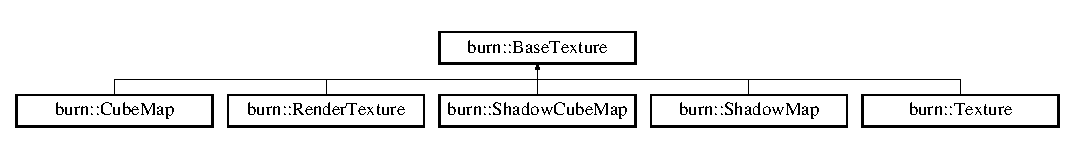
\includegraphics[height=1.473684cm]{classburn_1_1_base_texture}
\end{center}
\end{figure}
\subsection*{Public Member Functions}
\begin{DoxyCompactItemize}
\item 
\hyperlink{classburn_1_1_base_texture_a7aaaf6a1bd92d7efbf924255f10d31ad}{Base\-Texture} ()
\item 
virtual \hyperlink{classburn_1_1_base_texture_a054138cc6815ce69a61d9a3562f40a97}{$\sim$\-Base\-Texture} ()
\item 
void \hyperlink{classburn_1_1_base_texture_a4e586c45bf9b0936c17b2fa86aafad9b}{bind\-As\-Source} (const unsigned int \&unit=0) const 
\item 
void \hyperlink{classburn_1_1_base_texture_a88f83680c883f5962394061104a6c1c0}{unbind\-As\-Source} (const unsigned int \&unit=0) const 
\item 
bool \hyperlink{classburn_1_1_base_texture_afacc4aec15130a7b9b938bb7e8af1b07}{set\-Filtering} (const \hyperlink{classburn_1_1_sampler_a09433eae16f8623591d415a3f8c6afec}{Sampler\-::\-Magnification\-Filtering} \&mag, const \hyperlink{classburn_1_1_sampler_a09d6e36f45577a56ce230549aeaaab10}{Sampler\-::\-Minification\-Filtering} \&min)
\item 
bool \hyperlink{classburn_1_1_base_texture_acc07ff83e953a842ed65576ccc8a30e5}{set\-Sampler\-Parameter} (G\-Lenum parameter, G\-Lenum value)
\item 
bool \hyperlink{classburn_1_1_base_texture_a7b1590c284aa57ce7776eb294abd75ae}{set\-Anisotropic\-Level} (const G\-Lfloat \&level)
\end{DoxyCompactItemize}
\subsection*{Static Public Member Functions}
\begin{DoxyCompactItemize}
\item 
static \hyperlink{namespaceburn_a6805fa33c49c4c3db88a7bebba2c408f}{Vector2ui} \hyperlink{classburn_1_1_base_texture_a554f635fcec7c6d41aef0449991b5b1d}{calculate\-Pow2\-Dimensions} (const \hyperlink{namespaceburn_a6805fa33c49c4c3db88a7bebba2c408f}{Vector2ui} \&dimensions)
\end{DoxyCompactItemize}
\subsection*{Protected Member Functions}
\begin{DoxyCompactItemize}
\item 
virtual void \hyperlink{classburn_1_1_base_texture_a1102bd72393ccc77bd1fc47e046b4900}{on\-Bind} (const unsigned int \&unit) const =0
\item 
virtual void \hyperlink{classburn_1_1_base_texture_a06c69280f4bed1ac923cfeacad6a2aa6}{on\-Unbind} (const unsigned int \&unit) const =0
\end{DoxyCompactItemize}


\subsection{Constructor \& Destructor Documentation}
\hypertarget{classburn_1_1_base_texture_a7aaaf6a1bd92d7efbf924255f10d31ad}{\index{burn\-::\-Base\-Texture@{burn\-::\-Base\-Texture}!Base\-Texture@{Base\-Texture}}
\index{Base\-Texture@{Base\-Texture}!burn::BaseTexture@{burn\-::\-Base\-Texture}}
\subsubsection[{Base\-Texture}]{\setlength{\rightskip}{0pt plus 5cm}burn\-::\-Base\-Texture\-::\-Base\-Texture (
\begin{DoxyParamCaption}
{}
\end{DoxyParamCaption}
)}}\label{classburn_1_1_base_texture_a7aaaf6a1bd92d7efbf924255f10d31ad}
\hypertarget{classburn_1_1_base_texture_a054138cc6815ce69a61d9a3562f40a97}{\index{burn\-::\-Base\-Texture@{burn\-::\-Base\-Texture}!$\sim$\-Base\-Texture@{$\sim$\-Base\-Texture}}
\index{$\sim$\-Base\-Texture@{$\sim$\-Base\-Texture}!burn::BaseTexture@{burn\-::\-Base\-Texture}}
\subsubsection[{$\sim$\-Base\-Texture}]{\setlength{\rightskip}{0pt plus 5cm}virtual burn\-::\-Base\-Texture\-::$\sim$\-Base\-Texture (
\begin{DoxyParamCaption}
{}
\end{DoxyParamCaption}
)\hspace{0.3cm}{\ttfamily [virtual]}}}\label{classburn_1_1_base_texture_a054138cc6815ce69a61d9a3562f40a97}


\subsection{Member Function Documentation}
\hypertarget{classburn_1_1_base_texture_a4e586c45bf9b0936c17b2fa86aafad9b}{\index{burn\-::\-Base\-Texture@{burn\-::\-Base\-Texture}!bind\-As\-Source@{bind\-As\-Source}}
\index{bind\-As\-Source@{bind\-As\-Source}!burn::BaseTexture@{burn\-::\-Base\-Texture}}
\subsubsection[{bind\-As\-Source}]{\setlength{\rightskip}{0pt plus 5cm}void burn\-::\-Base\-Texture\-::bind\-As\-Source (
\begin{DoxyParamCaption}
\item[{const unsigned int \&}]{unit = {\ttfamily 0}}
\end{DoxyParamCaption}
) const}}\label{classburn_1_1_base_texture_a4e586c45bf9b0936c17b2fa86aafad9b}
\hypertarget{classburn_1_1_base_texture_a554f635fcec7c6d41aef0449991b5b1d}{\index{burn\-::\-Base\-Texture@{burn\-::\-Base\-Texture}!calculate\-Pow2\-Dimensions@{calculate\-Pow2\-Dimensions}}
\index{calculate\-Pow2\-Dimensions@{calculate\-Pow2\-Dimensions}!burn::BaseTexture@{burn\-::\-Base\-Texture}}
\subsubsection[{calculate\-Pow2\-Dimensions}]{\setlength{\rightskip}{0pt plus 5cm}static {\bf Vector2ui} burn\-::\-Base\-Texture\-::calculate\-Pow2\-Dimensions (
\begin{DoxyParamCaption}
\item[{const {\bf Vector2ui} \&}]{dimensions}
\end{DoxyParamCaption}
)\hspace{0.3cm}{\ttfamily [static]}}}\label{classburn_1_1_base_texture_a554f635fcec7c6d41aef0449991b5b1d}
\hypertarget{classburn_1_1_base_texture_a1102bd72393ccc77bd1fc47e046b4900}{\index{burn\-::\-Base\-Texture@{burn\-::\-Base\-Texture}!on\-Bind@{on\-Bind}}
\index{on\-Bind@{on\-Bind}!burn::BaseTexture@{burn\-::\-Base\-Texture}}
\subsubsection[{on\-Bind}]{\setlength{\rightskip}{0pt plus 5cm}virtual void burn\-::\-Base\-Texture\-::on\-Bind (
\begin{DoxyParamCaption}
\item[{const unsigned int \&}]{unit}
\end{DoxyParamCaption}
) const\hspace{0.3cm}{\ttfamily [protected]}, {\ttfamily [pure virtual]}}}\label{classburn_1_1_base_texture_a1102bd72393ccc77bd1fc47e046b4900}


Implemented in \hyperlink{classburn_1_1_texture_a41cf19a71e61bb8ddfd6bf93d1c0ef02}{burn\-::\-Texture}.

\hypertarget{classburn_1_1_base_texture_a06c69280f4bed1ac923cfeacad6a2aa6}{\index{burn\-::\-Base\-Texture@{burn\-::\-Base\-Texture}!on\-Unbind@{on\-Unbind}}
\index{on\-Unbind@{on\-Unbind}!burn::BaseTexture@{burn\-::\-Base\-Texture}}
\subsubsection[{on\-Unbind}]{\setlength{\rightskip}{0pt plus 5cm}virtual void burn\-::\-Base\-Texture\-::on\-Unbind (
\begin{DoxyParamCaption}
\item[{const unsigned int \&}]{unit}
\end{DoxyParamCaption}
) const\hspace{0.3cm}{\ttfamily [protected]}, {\ttfamily [pure virtual]}}}\label{classburn_1_1_base_texture_a06c69280f4bed1ac923cfeacad6a2aa6}


Implemented in \hyperlink{classburn_1_1_texture_a1a2a5e886e044ac83fa575916129884f}{burn\-::\-Texture}.

\hypertarget{classburn_1_1_base_texture_a7b1590c284aa57ce7776eb294abd75ae}{\index{burn\-::\-Base\-Texture@{burn\-::\-Base\-Texture}!set\-Anisotropic\-Level@{set\-Anisotropic\-Level}}
\index{set\-Anisotropic\-Level@{set\-Anisotropic\-Level}!burn::BaseTexture@{burn\-::\-Base\-Texture}}
\subsubsection[{set\-Anisotropic\-Level}]{\setlength{\rightskip}{0pt plus 5cm}bool burn\-::\-Base\-Texture\-::set\-Anisotropic\-Level (
\begin{DoxyParamCaption}
\item[{const G\-Lfloat \&}]{level}
\end{DoxyParamCaption}
)}}\label{classburn_1_1_base_texture_a7b1590c284aa57ce7776eb294abd75ae}
\hypertarget{classburn_1_1_base_texture_afacc4aec15130a7b9b938bb7e8af1b07}{\index{burn\-::\-Base\-Texture@{burn\-::\-Base\-Texture}!set\-Filtering@{set\-Filtering}}
\index{set\-Filtering@{set\-Filtering}!burn::BaseTexture@{burn\-::\-Base\-Texture}}
\subsubsection[{set\-Filtering}]{\setlength{\rightskip}{0pt plus 5cm}bool burn\-::\-Base\-Texture\-::set\-Filtering (
\begin{DoxyParamCaption}
\item[{const {\bf Sampler\-::\-Magnification\-Filtering} \&}]{mag, }
\item[{const {\bf Sampler\-::\-Minification\-Filtering} \&}]{min}
\end{DoxyParamCaption}
)}}\label{classburn_1_1_base_texture_afacc4aec15130a7b9b938bb7e8af1b07}
\hypertarget{classburn_1_1_base_texture_acc07ff83e953a842ed65576ccc8a30e5}{\index{burn\-::\-Base\-Texture@{burn\-::\-Base\-Texture}!set\-Sampler\-Parameter@{set\-Sampler\-Parameter}}
\index{set\-Sampler\-Parameter@{set\-Sampler\-Parameter}!burn::BaseTexture@{burn\-::\-Base\-Texture}}
\subsubsection[{set\-Sampler\-Parameter}]{\setlength{\rightskip}{0pt plus 5cm}bool burn\-::\-Base\-Texture\-::set\-Sampler\-Parameter (
\begin{DoxyParamCaption}
\item[{G\-Lenum}]{parameter, }
\item[{G\-Lenum}]{value}
\end{DoxyParamCaption}
)}}\label{classburn_1_1_base_texture_acc07ff83e953a842ed65576ccc8a30e5}
\hypertarget{classburn_1_1_base_texture_a88f83680c883f5962394061104a6c1c0}{\index{burn\-::\-Base\-Texture@{burn\-::\-Base\-Texture}!unbind\-As\-Source@{unbind\-As\-Source}}
\index{unbind\-As\-Source@{unbind\-As\-Source}!burn::BaseTexture@{burn\-::\-Base\-Texture}}
\subsubsection[{unbind\-As\-Source}]{\setlength{\rightskip}{0pt plus 5cm}void burn\-::\-Base\-Texture\-::unbind\-As\-Source (
\begin{DoxyParamCaption}
\item[{const unsigned int \&}]{unit = {\ttfamily 0}}
\end{DoxyParamCaption}
) const}}\label{classburn_1_1_base_texture_a88f83680c883f5962394061104a6c1c0}


The documentation for this class was generated from the following file\-:\begin{DoxyCompactItemize}
\item 
include/\-Burngine/\-Graphics/\-Texture/\hyperlink{_base_texture_8h}{Base\-Texture.\-h}\end{DoxyCompactItemize}

\hypertarget{structburn_1_1_burngine_shaders}{\section{burn\-:\-:Burngine\-Shaders Struct Reference}
\label{structburn_1_1_burngine_shaders}\index{burn\-::\-Burngine\-Shaders@{burn\-::\-Burngine\-Shaders}}
}


{\ttfamily \#include $<$Shader.\-h$>$}

\subsection*{Public Types}
\begin{DoxyCompactItemize}
\item 
enum \hyperlink{structburn_1_1_burngine_shaders_a2c339d4b838b7efe94ba8ef7f480ef41}{Type} \{ \\*
\hyperlink{structburn_1_1_burngine_shaders_a2c339d4b838b7efe94ba8ef7f480ef41a88513d98f02053992a4d753db14104e1}{S\-O\-L\-I\-D\-\_\-\-C\-O\-L\-O\-R}, 
\hyperlink{structburn_1_1_burngine_shaders_a2c339d4b838b7efe94ba8ef7f480ef41a9bd651b914b48fcb7a4a64c3f6e4111a}{T\-E\-X\-T\-U\-R\-E\-D}, 
\hyperlink{structburn_1_1_burngine_shaders_a2c339d4b838b7efe94ba8ef7f480ef41a53274ea9313d7d56a0c613f2f384d2c7}{R\-A\-W\-\_\-\-T\-E\-X\-T\-U\-R\-E}, 
\hyperlink{structburn_1_1_burngine_shaders_a2c339d4b838b7efe94ba8ef7f480ef41ac7bc9acc35a1eb3a3839b8fe6ead3c9f}{L\-I\-G\-H\-T\-I\-N\-G}, 
\\*
\hyperlink{structburn_1_1_burngine_shaders_a2c339d4b838b7efe94ba8ef7f480ef41a2b9f8e6b326d31ef61c68231aa0a37eb}{C\-O\-L\-O\-R\-L\-E\-S\-S}
 \}
\begin{DoxyCompactList}\small\item\em Enum for several predefined shaders. \end{DoxyCompactList}\end{DoxyCompactItemize}
\subsection*{Public Member Functions}
\begin{DoxyCompactItemize}
\item 
\hyperlink{structburn_1_1_burngine_shaders_a7839e417fb8b954b87ece696e48041eb}{Burngine\-Shaders} ()=delete
\begin{DoxyCompactList}\small\item\em Constructor is deleted, because this is a static struct. \end{DoxyCompactList}\end{DoxyCompactItemize}
\subsection*{Static Public Member Functions}
\begin{DoxyCompactItemize}
\item 
static bool \hyperlink{structburn_1_1_burngine_shaders_ab9ebed7c4668a72e7cbbd0630226d7ab}{load\-Shader} (const \hyperlink{structburn_1_1_burngine_shaders_a2c339d4b838b7efe94ba8ef7f480ef41}{Type} \&type)
\begin{DoxyCompactList}\small\item\em Loads and creates a predefined shader. \end{DoxyCompactList}\item 
static bool \hyperlink{structburn_1_1_burngine_shaders_a33e19e46e7bc1b6d18f05d2ee233dc50}{load\-All\-Shaders} ()
\begin{DoxyCompactList}\small\item\em Loads and creates all predefined shaders. \end{DoxyCompactList}\item 
static void \hyperlink{structburn_1_1_burngine_shaders_a73204821ded279b767394accf6f7ee75}{use\-Shader} (const \hyperlink{structburn_1_1_burngine_shaders_a2c339d4b838b7efe94ba8ef7f480ef41}{Type} \&type)
\begin{DoxyCompactList}\small\item\em Activates a predefined shader. \end{DoxyCompactList}\item 
static G\-Luint \hyperlink{structburn_1_1_burngine_shaders_adcd311730ecd21d2729199952a5bdf11}{get\-Shader\-Uniform\-Location} (const \hyperlink{structburn_1_1_burngine_shaders_a2c339d4b838b7efe94ba8ef7f480ef41}{Type} \&type, const std\-::string \&uniform\-Name)
\begin{DoxyCompactList}\small\item\em Does the same like \hyperlink{classburn_1_1_shader_ae96b86c6da489d759bec9be7664040dc}{Shader\-::get\-Uniform\-Location()} but on the predefined ones. \end{DoxyCompactList}\end{DoxyCompactItemize}


\subsection{Member Enumeration Documentation}
\hypertarget{structburn_1_1_burngine_shaders_a2c339d4b838b7efe94ba8ef7f480ef41}{\index{burn\-::\-Burngine\-Shaders@{burn\-::\-Burngine\-Shaders}!Type@{Type}}
\index{Type@{Type}!burn::BurngineShaders@{burn\-::\-Burngine\-Shaders}}
\subsubsection[{Type}]{\setlength{\rightskip}{0pt plus 5cm}enum {\bf burn\-::\-Burngine\-Shaders\-::\-Type}}}\label{structburn_1_1_burngine_shaders_a2c339d4b838b7efe94ba8ef7f480ef41}


Enum for several predefined shaders. 

\begin{DoxySeeAlso}{See Also}
\hyperlink{structburn_1_1_burngine_shaders_ab9ebed7c4668a72e7cbbd0630226d7ab}{load\-Shader()} 

\hyperlink{structburn_1_1_burngine_shaders_a73204821ded279b767394accf6f7ee75}{use\-Shader()} 
\end{DoxySeeAlso}
\begin{Desc}
\item[Enumerator]\par
\begin{description}
\index{S\-O\-L\-I\-D\-\_\-\-C\-O\-L\-O\-R@{S\-O\-L\-I\-D\-\_\-\-C\-O\-L\-O\-R}!burn\-::\-Burngine\-Shaders@{burn\-::\-Burngine\-Shaders}}\index{burn\-::\-Burngine\-Shaders@{burn\-::\-Burngine\-Shaders}!S\-O\-L\-I\-D\-\_\-\-C\-O\-L\-O\-R@{S\-O\-L\-I\-D\-\_\-\-C\-O\-L\-O\-R}}\item[{\em 
\hypertarget{structburn_1_1_burngine_shaders_a2c339d4b838b7efe94ba8ef7f480ef41a88513d98f02053992a4d753db14104e1}{S\-O\-L\-I\-D\-\_\-\-C\-O\-L\-O\-R}\label{structburn_1_1_burngine_shaders_a2c339d4b838b7efe94ba8ef7f480ef41a88513d98f02053992a4d753db14104e1}
}]Solid Color \hyperlink{classburn_1_1_shader}{Shader}. \index{T\-E\-X\-T\-U\-R\-E\-D@{T\-E\-X\-T\-U\-R\-E\-D}!burn\-::\-Burngine\-Shaders@{burn\-::\-Burngine\-Shaders}}\index{burn\-::\-Burngine\-Shaders@{burn\-::\-Burngine\-Shaders}!T\-E\-X\-T\-U\-R\-E\-D@{T\-E\-X\-T\-U\-R\-E\-D}}\item[{\em 
\hypertarget{structburn_1_1_burngine_shaders_a2c339d4b838b7efe94ba8ef7f480ef41a9bd651b914b48fcb7a4a64c3f6e4111a}{T\-E\-X\-T\-U\-R\-E\-D}\label{structburn_1_1_burngine_shaders_a2c339d4b838b7efe94ba8ef7f480ef41a9bd651b914b48fcb7a4a64c3f6e4111a}
}]Simple 1-\/\-Texture \hyperlink{classburn_1_1_shader}{Shader}. \index{R\-A\-W\-\_\-\-T\-E\-X\-T\-U\-R\-E@{R\-A\-W\-\_\-\-T\-E\-X\-T\-U\-R\-E}!burn\-::\-Burngine\-Shaders@{burn\-::\-Burngine\-Shaders}}\index{burn\-::\-Burngine\-Shaders@{burn\-::\-Burngine\-Shaders}!R\-A\-W\-\_\-\-T\-E\-X\-T\-U\-R\-E@{R\-A\-W\-\_\-\-T\-E\-X\-T\-U\-R\-E}}\item[{\em 
\hypertarget{structburn_1_1_burngine_shaders_a2c339d4b838b7efe94ba8ef7f480ef41a53274ea9313d7d56a0c613f2f384d2c7}{R\-A\-W\-\_\-\-T\-E\-X\-T\-U\-R\-E}\label{structburn_1_1_burngine_shaders_a2c339d4b838b7efe94ba8ef7f480ef41a53274ea9313d7d56a0c613f2f384d2c7}
}]This renders a texture without matrices. (Internal use) \index{L\-I\-G\-H\-T\-I\-N\-G@{L\-I\-G\-H\-T\-I\-N\-G}!burn\-::\-Burngine\-Shaders@{burn\-::\-Burngine\-Shaders}}\index{burn\-::\-Burngine\-Shaders@{burn\-::\-Burngine\-Shaders}!L\-I\-G\-H\-T\-I\-N\-G@{L\-I\-G\-H\-T\-I\-N\-G}}\item[{\em 
\hypertarget{structburn_1_1_burngine_shaders_a2c339d4b838b7efe94ba8ef7f480ef41ac7bc9acc35a1eb3a3839b8fe6ead3c9f}{L\-I\-G\-H\-T\-I\-N\-G}\label{structburn_1_1_burngine_shaders_a2c339d4b838b7efe94ba8ef7f480ef41ac7bc9acc35a1eb3a3839b8fe6ead3c9f}
}]Renders the model's lighting. \index{C\-O\-L\-O\-R\-L\-E\-S\-S@{C\-O\-L\-O\-R\-L\-E\-S\-S}!burn\-::\-Burngine\-Shaders@{burn\-::\-Burngine\-Shaders}}\index{burn\-::\-Burngine\-Shaders@{burn\-::\-Burngine\-Shaders}!C\-O\-L\-O\-R\-L\-E\-S\-S@{C\-O\-L\-O\-R\-L\-E\-S\-S}}\item[{\em 
\hypertarget{structburn_1_1_burngine_shaders_a2c339d4b838b7efe94ba8ef7f480ef41a2b9f8e6b326d31ef61c68231aa0a37eb}{C\-O\-L\-O\-R\-L\-E\-S\-S}\label{structburn_1_1_burngine_shaders_a2c339d4b838b7efe94ba8ef7f480ef41a2b9f8e6b326d31ef61c68231aa0a37eb}
}]Draws only black color (internal use for depthbufferwriting) \end{description}
\end{Desc}


\subsection{Constructor \& Destructor Documentation}
\hypertarget{structburn_1_1_burngine_shaders_a7839e417fb8b954b87ece696e48041eb}{\index{burn\-::\-Burngine\-Shaders@{burn\-::\-Burngine\-Shaders}!Burngine\-Shaders@{Burngine\-Shaders}}
\index{Burngine\-Shaders@{Burngine\-Shaders}!burn::BurngineShaders@{burn\-::\-Burngine\-Shaders}}
\subsubsection[{Burngine\-Shaders}]{\setlength{\rightskip}{0pt plus 5cm}burn\-::\-Burngine\-Shaders\-::\-Burngine\-Shaders (
\begin{DoxyParamCaption}
{}
\end{DoxyParamCaption}
)\hspace{0.3cm}{\ttfamily [delete]}}}\label{structburn_1_1_burngine_shaders_a7839e417fb8b954b87ece696e48041eb}


Constructor is deleted, because this is a static struct. 



\subsection{Member Function Documentation}
\hypertarget{structburn_1_1_burngine_shaders_adcd311730ecd21d2729199952a5bdf11}{\index{burn\-::\-Burngine\-Shaders@{burn\-::\-Burngine\-Shaders}!get\-Shader\-Uniform\-Location@{get\-Shader\-Uniform\-Location}}
\index{get\-Shader\-Uniform\-Location@{get\-Shader\-Uniform\-Location}!burn::BurngineShaders@{burn\-::\-Burngine\-Shaders}}
\subsubsection[{get\-Shader\-Uniform\-Location}]{\setlength{\rightskip}{0pt plus 5cm}G\-Luint burn\-::\-Burngine\-Shaders\-::get\-Shader\-Uniform\-Location (
\begin{DoxyParamCaption}
\item[{const {\bf Type} \&}]{type, }
\item[{const std\-::string \&}]{uniform\-Name}
\end{DoxyParamCaption}
)\hspace{0.3cm}{\ttfamily [static]}}}\label{structburn_1_1_burngine_shaders_adcd311730ecd21d2729199952a5bdf11}


Does the same like \hyperlink{classburn_1_1_shader_ae96b86c6da489d759bec9be7664040dc}{Shader\-::get\-Uniform\-Location()} but on the predefined ones. 


\begin{DoxyParams}{Parameters}
{\em type} & The shader in which the uniform will be searched \\
\hline
{\em uniform\-Name} & The uniform name in the shaderprogram\\
\hline
\end{DoxyParams}
\begin{DoxyReturn}{Returns}
Returns the position of the uniform or -\/1 when failed
\end{DoxyReturn}
\begin{DoxySeeAlso}{See Also}
\hyperlink{classburn_1_1_shader_ae96b86c6da489d759bec9be7664040dc}{Shader\-::get\-Uniform\-Location()} 
\end{DoxySeeAlso}
\hypertarget{structburn_1_1_burngine_shaders_a33e19e46e7bc1b6d18f05d2ee233dc50}{\index{burn\-::\-Burngine\-Shaders@{burn\-::\-Burngine\-Shaders}!load\-All\-Shaders@{load\-All\-Shaders}}
\index{load\-All\-Shaders@{load\-All\-Shaders}!burn::BurngineShaders@{burn\-::\-Burngine\-Shaders}}
\subsubsection[{load\-All\-Shaders}]{\setlength{\rightskip}{0pt plus 5cm}bool burn\-::\-Burngine\-Shaders\-::load\-All\-Shaders (
\begin{DoxyParamCaption}
{}
\end{DoxyParamCaption}
)\hspace{0.3cm}{\ttfamily [static]}}}\label{structburn_1_1_burngine_shaders_a33e19e46e7bc1b6d18f05d2ee233dc50}


Loads and creates all predefined shaders. 

\begin{DoxySeeAlso}{See Also}
\hyperlink{structburn_1_1_burngine_shaders_ab9ebed7c4668a72e7cbbd0630226d7ab}{load\-Shader()} 
\end{DoxySeeAlso}
\hypertarget{structburn_1_1_burngine_shaders_ab9ebed7c4668a72e7cbbd0630226d7ab}{\index{burn\-::\-Burngine\-Shaders@{burn\-::\-Burngine\-Shaders}!load\-Shader@{load\-Shader}}
\index{load\-Shader@{load\-Shader}!burn::BurngineShaders@{burn\-::\-Burngine\-Shaders}}
\subsubsection[{load\-Shader}]{\setlength{\rightskip}{0pt plus 5cm}bool burn\-::\-Burngine\-Shaders\-::load\-Shader (
\begin{DoxyParamCaption}
\item[{const {\bf Type} \&}]{type}
\end{DoxyParamCaption}
)\hspace{0.3cm}{\ttfamily [static]}}}\label{structburn_1_1_burngine_shaders_ab9ebed7c4668a72e7cbbd0630226d7ab}


Loads and creates a predefined shader. 


\begin{DoxyParams}{Parameters}
{\em type} & The shader to load/create.\\
\hline
\end{DoxyParams}
\begin{DoxyReturn}{Returns}
Returns true on success.
\end{DoxyReturn}
\begin{DoxySeeAlso}{See Also}
\hyperlink{structburn_1_1_burngine_shaders_a33e19e46e7bc1b6d18f05d2ee233dc50}{load\-All\-Shaders()} 

\hyperlink{structburn_1_1_burngine_shaders_a73204821ded279b767394accf6f7ee75}{use\-Shader()} 

\hyperlink{structburn_1_1_burngine_shaders_a2c339d4b838b7efe94ba8ef7f480ef41}{Type} 
\end{DoxySeeAlso}
\hypertarget{structburn_1_1_burngine_shaders_a73204821ded279b767394accf6f7ee75}{\index{burn\-::\-Burngine\-Shaders@{burn\-::\-Burngine\-Shaders}!use\-Shader@{use\-Shader}}
\index{use\-Shader@{use\-Shader}!burn::BurngineShaders@{burn\-::\-Burngine\-Shaders}}
\subsubsection[{use\-Shader}]{\setlength{\rightskip}{0pt plus 5cm}void burn\-::\-Burngine\-Shaders\-::use\-Shader (
\begin{DoxyParamCaption}
\item[{const {\bf Type} \&}]{type}
\end{DoxyParamCaption}
)\hspace{0.3cm}{\ttfamily [static]}}}\label{structburn_1_1_burngine_shaders_a73204821ded279b767394accf6f7ee75}


Activates a predefined shader. 


\begin{DoxyParams}{Parameters}
{\em type} & The shader to activate.\\
\hline
\end{DoxyParams}
\begin{DoxyNote}{Note}
Ensure that the predefined shader has been loaded!
\end{DoxyNote}
\begin{DoxySeeAlso}{See Also}
\hyperlink{structburn_1_1_burngine_shaders_ab9ebed7c4668a72e7cbbd0630226d7ab}{load\-Shader()} 

\hyperlink{structburn_1_1_burngine_shaders_a33e19e46e7bc1b6d18f05d2ee233dc50}{load\-All\-Shaders()} 
\end{DoxySeeAlso}


The documentation for this struct was generated from the following files\-:\begin{DoxyCompactItemize}
\item 
include/\-Burngine/\-Graphics/\hyperlink{_shader_8h}{Shader.\-h}\item 
include/\-Burngine/\-Graphics/\hyperlink{_shader_8cpp}{Shader.\-cpp}\end{DoxyCompactItemize}

\hypertarget{classburn_1_1_camera}{\section{burn\-:\-:Camera Class Reference}
\label{classburn_1_1_camera}\index{burn\-::\-Camera@{burn\-::\-Camera}}
}


{\ttfamily \#include $<$Camera.\-h$>$}

Inheritance diagram for burn\-:\-:Camera\-:\begin{figure}[H]
\begin{center}
\leavevmode
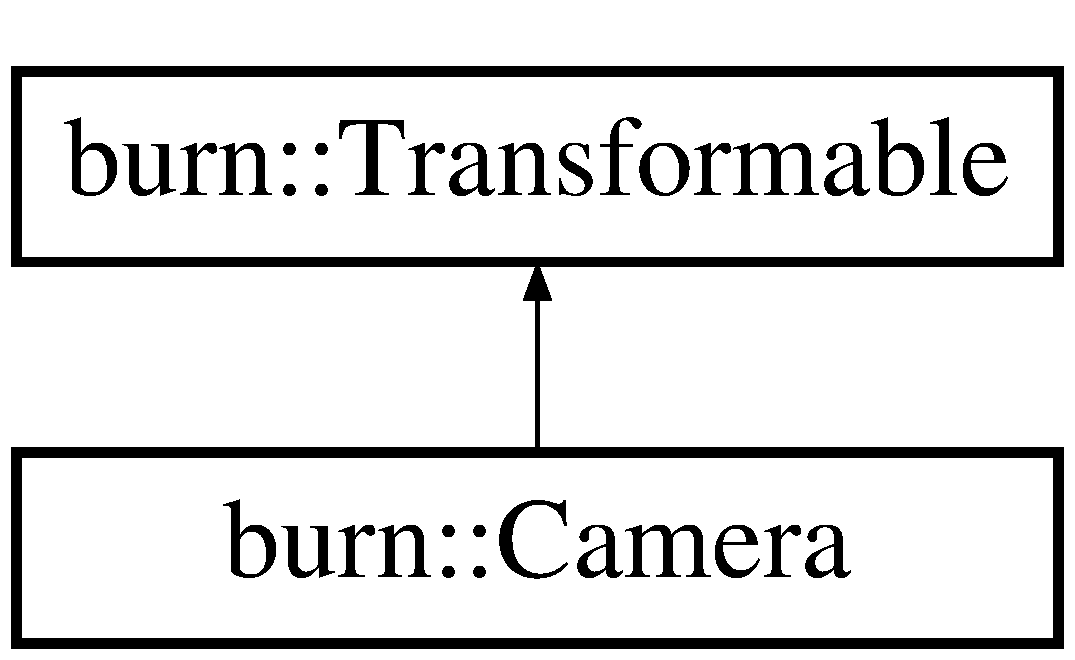
\includegraphics[height=2.000000cm]{classburn_1_1_camera}
\end{center}
\end{figure}
\subsection*{Public Member Functions}
\begin{DoxyCompactItemize}
\item 
\hyperlink{classburn_1_1_camera_aa0eac6e197cfbebe709b524eae890a02}{Camera} ()
\begin{DoxyCompactList}\small\item\em Default Contstructor of \hyperlink{classburn_1_1_camera}{Camera}. Default values\-: \end{DoxyCompactList}\item 
\hyperlink{classburn_1_1_camera_a717df173cafcdce81c01eb6744332ae7}{$\sim$\-Camera} ()
\begin{DoxyCompactList}\small\item\em Default Destructor. \end{DoxyCompactList}\item 
void \hyperlink{classburn_1_1_camera_ac3ebe6eb9c44fe8068e397c8e22b5c72}{set\-Aspect\-Ratio} (const float \&aspect\-Ratio)
\begin{DoxyCompactList}\small\item\em Changes the aspectratio that the scene will be drawn with. \end{DoxyCompactList}\item 
const float \& \hyperlink{classburn_1_1_camera_a0867612bbd199c663e477ffe68e989f6}{get\-Aspect\-Ratio} () const 
\begin{DoxyCompactList}\small\item\em Returns the current aspectratio. \end{DoxyCompactList}\item 
void \hyperlink{classburn_1_1_camera_aacfbde225b770a51a020ec15403b1c41}{look\-At} (const \hyperlink{namespaceburn_afdd7cfb352b9612432faf6947b6fff74}{Vector3f} \&point)
\begin{DoxyCompactList}\small\item\em Sets the point the camera will face to. \end{DoxyCompactList}\item 
const \hyperlink{namespaceburn_afdd7cfb352b9612432faf6947b6fff74}{Vector3f} \& \hyperlink{classburn_1_1_camera_a6e2e4ace192d77e5a9d9b62d2c2915da}{get\-Look\-At} () const 
\begin{DoxyCompactList}\small\item\em Returns the point the camera is facing. \end{DoxyCompactList}\item 
void \hyperlink{classburn_1_1_camera_a075d0fa32315aa3b9c55a2fa5135bdfd}{set\-Fov} (const float \&fov)
\begin{DoxyCompactList}\small\item\em Sets the Field-\/\-Of-\/\-View. \end{DoxyCompactList}\item 
const float \& \hyperlink{classburn_1_1_camera_ac74fe26c2f2b0d762e5886fa8ab1f97f}{get\-Fov} () const 
\begin{DoxyCompactList}\small\item\em Returns the current Field-\/\-Of-\/\-View. \end{DoxyCompactList}\end{DoxyCompactItemize}
\subsection*{Additional Inherited Members}


\subsection{Constructor \& Destructor Documentation}
\hypertarget{classburn_1_1_camera_aa0eac6e197cfbebe709b524eae890a02}{\index{burn\-::\-Camera@{burn\-::\-Camera}!Camera@{Camera}}
\index{Camera@{Camera}!burn::Camera@{burn\-::\-Camera}}
\subsubsection[{Camera}]{\setlength{\rightskip}{0pt plus 5cm}burn\-::\-Camera\-::\-Camera (
\begin{DoxyParamCaption}
{}
\end{DoxyParamCaption}
)}}\label{classburn_1_1_camera_aa0eac6e197cfbebe709b524eae890a02}


Default Contstructor of \hyperlink{classburn_1_1_camera}{Camera}. Default values\-: 


\begin{DoxyItemize}
\item Aspect\-Ratio\-: 16/9
\item Look\-At\-: 0/0/0 (Origin)
\item F\-O\-V\-: 45
\end{DoxyItemize}

\begin{DoxyNote}{Note}
In order to see results by changing values, ensure that your camera is active. 
\end{DoxyNote}
\hypertarget{classburn_1_1_camera_a717df173cafcdce81c01eb6744332ae7}{\index{burn\-::\-Camera@{burn\-::\-Camera}!$\sim$\-Camera@{$\sim$\-Camera}}
\index{$\sim$\-Camera@{$\sim$\-Camera}!burn::Camera@{burn\-::\-Camera}}
\subsubsection[{$\sim$\-Camera}]{\setlength{\rightskip}{0pt plus 5cm}burn\-::\-Camera\-::$\sim$\-Camera (
\begin{DoxyParamCaption}
{}
\end{DoxyParamCaption}
)}}\label{classburn_1_1_camera_a717df173cafcdce81c01eb6744332ae7}


Default Destructor. 

\begin{DoxyNote}{Note}
Make sure to delete the camera with Scene\-::remove\-Camera() when you have created it with Scene\-::create\-Camera() ! 
\end{DoxyNote}


\subsection{Member Function Documentation}
\hypertarget{classburn_1_1_camera_a0867612bbd199c663e477ffe68e989f6}{\index{burn\-::\-Camera@{burn\-::\-Camera}!get\-Aspect\-Ratio@{get\-Aspect\-Ratio}}
\index{get\-Aspect\-Ratio@{get\-Aspect\-Ratio}!burn::Camera@{burn\-::\-Camera}}
\subsubsection[{get\-Aspect\-Ratio}]{\setlength{\rightskip}{0pt plus 5cm}const float\& burn\-::\-Camera\-::get\-Aspect\-Ratio (
\begin{DoxyParamCaption}
{}
\end{DoxyParamCaption}
) const}}\label{classburn_1_1_camera_a0867612bbd199c663e477ffe68e989f6}


Returns the current aspectratio. 

\begin{DoxyReturn}{Returns}
The current Aspect\-Ratio
\end{DoxyReturn}
\hyperlink{classburn_1_1_camera_ac3ebe6eb9c44fe8068e397c8e22b5c72}{set\-Aspect\-Ratio()} \hypertarget{classburn_1_1_camera_ac74fe26c2f2b0d762e5886fa8ab1f97f}{\index{burn\-::\-Camera@{burn\-::\-Camera}!get\-Fov@{get\-Fov}}
\index{get\-Fov@{get\-Fov}!burn::Camera@{burn\-::\-Camera}}
\subsubsection[{get\-Fov}]{\setlength{\rightskip}{0pt plus 5cm}const float\& burn\-::\-Camera\-::get\-Fov (
\begin{DoxyParamCaption}
{}
\end{DoxyParamCaption}
) const}}\label{classburn_1_1_camera_ac74fe26c2f2b0d762e5886fa8ab1f97f}


Returns the current Field-\/\-Of-\/\-View. 

\begin{DoxyReturn}{Returns}
A value between 0 and 90 
\end{DoxyReturn}
\hypertarget{classburn_1_1_camera_a6e2e4ace192d77e5a9d9b62d2c2915da}{\index{burn\-::\-Camera@{burn\-::\-Camera}!get\-Look\-At@{get\-Look\-At}}
\index{get\-Look\-At@{get\-Look\-At}!burn::Camera@{burn\-::\-Camera}}
\subsubsection[{get\-Look\-At}]{\setlength{\rightskip}{0pt plus 5cm}const {\bf Vector3f}\& burn\-::\-Camera\-::get\-Look\-At (
\begin{DoxyParamCaption}
{}
\end{DoxyParamCaption}
) const}}\label{classburn_1_1_camera_a6e2e4ace192d77e5a9d9b62d2c2915da}


Returns the point the camera is facing. 

\begin{DoxyReturn}{Returns}
A Vector3f defining the faced point
\end{DoxyReturn}
\begin{DoxySeeAlso}{See Also}
\hyperlink{classburn_1_1_camera_aacfbde225b770a51a020ec15403b1c41}{look\-At()} 
\end{DoxySeeAlso}
\hypertarget{classburn_1_1_camera_aacfbde225b770a51a020ec15403b1c41}{\index{burn\-::\-Camera@{burn\-::\-Camera}!look\-At@{look\-At}}
\index{look\-At@{look\-At}!burn::Camera@{burn\-::\-Camera}}
\subsubsection[{look\-At}]{\setlength{\rightskip}{0pt plus 5cm}void burn\-::\-Camera\-::look\-At (
\begin{DoxyParamCaption}
\item[{const {\bf Vector3f} \&}]{point}
\end{DoxyParamCaption}
)}}\label{classburn_1_1_camera_aacfbde225b770a51a020ec15403b1c41}


Sets the point the camera will face to. 


\begin{DoxyParams}{Parameters}
{\em point} & A Vector3f defining the faced point\\
\hline
\end{DoxyParams}
\begin{DoxySeeAlso}{See Also}
\hyperlink{classburn_1_1_camera_a6e2e4ace192d77e5a9d9b62d2c2915da}{get\-Look\-At()} 
\end{DoxySeeAlso}
\hypertarget{classburn_1_1_camera_ac3ebe6eb9c44fe8068e397c8e22b5c72}{\index{burn\-::\-Camera@{burn\-::\-Camera}!set\-Aspect\-Ratio@{set\-Aspect\-Ratio}}
\index{set\-Aspect\-Ratio@{set\-Aspect\-Ratio}!burn::Camera@{burn\-::\-Camera}}
\subsubsection[{set\-Aspect\-Ratio}]{\setlength{\rightskip}{0pt plus 5cm}void burn\-::\-Camera\-::set\-Aspect\-Ratio (
\begin{DoxyParamCaption}
\item[{const float \&}]{aspect\-Ratio}
\end{DoxyParamCaption}
)}}\label{classburn_1_1_camera_ac3ebe6eb9c44fe8068e397c8e22b5c72}


Changes the aspectratio that the scene will be drawn with. 


\begin{DoxyParams}{Parameters}
{\em aspect\-Ratio} & The Aspect\-Ratio. Usually the width/height of the \hyperlink{classburn_1_1_window}{Window}\\
\hline
\end{DoxyParams}
\begin{DoxyNote}{Note}
Make sure to set your camera as active in order to see results.
\end{DoxyNote}
\begin{DoxySeeAlso}{See Also}
\hyperlink{classburn_1_1_camera_ac3ebe6eb9c44fe8068e397c8e22b5c72}{set\-Aspect\-Ratio()} 
\end{DoxySeeAlso}
\hypertarget{classburn_1_1_camera_a075d0fa32315aa3b9c55a2fa5135bdfd}{\index{burn\-::\-Camera@{burn\-::\-Camera}!set\-Fov@{set\-Fov}}
\index{set\-Fov@{set\-Fov}!burn::Camera@{burn\-::\-Camera}}
\subsubsection[{set\-Fov}]{\setlength{\rightskip}{0pt plus 5cm}void burn\-::\-Camera\-::set\-Fov (
\begin{DoxyParamCaption}
\item[{const float \&}]{fov}
\end{DoxyParamCaption}
)}}\label{classburn_1_1_camera_a075d0fa32315aa3b9c55a2fa5135bdfd}


Sets the Field-\/\-Of-\/\-View. 


\begin{DoxyParams}{Parameters}
{\em fov} & A value between 0 and 90 \\
\hline
\end{DoxyParams}


The documentation for this class was generated from the following file\-:\begin{DoxyCompactItemize}
\item 
include/\-Burngine/\-Graphics/\-Scene/\hyperlink{_camera_8h}{Camera.\-h}\end{DoxyCompactItemize}

\hypertarget{classburn_1_1_character}{\section{burn\-:\-:Character Class Reference}
\label{classburn_1_1_character}\index{burn\-::\-Character@{burn\-::\-Character}}
}


{\ttfamily \#include $<$Character.\-h$>$}

\subsection*{Public Member Functions}
\begin{DoxyCompactItemize}
\item 
\hyperlink{classburn_1_1_character_a9972c2e356b95364c64db345e69b8d23}{Character} (const \hyperlink{namespaceburn_ab40b09022209bd449d317c1f0e95356b}{Uint32} \&code\-Point=0, const unsigned int \&size=0)
\item 
\hyperlink{classburn_1_1_character_af8b977dc4ed78f7b45b673e339dbf7f5}{$\sim$\-Character} ()
\item 
void \hyperlink{classburn_1_1_character_a1d87ddcf0eb04b4153b5903c46ce2486}{create\-From\-Ft\-Glyph} (void $\ast$glyph, void $\ast$bitmap)
\item 
void \hyperlink{classburn_1_1_character_a1b8e1666f241a5b9d36a6ecc4aa9c6e4}{draw} (const \hyperlink{namespaceburn_af5ed9eb70cbf0fb572098ff43e146a0a}{Vector2f} \&position, const \hyperlink{namespaceburn_a58a411b9d83c7970518a9250c1c78068}{Vector4f} \&color) const 
\item 
bool \hyperlink{classburn_1_1_character_ae2ed0524994d3bcf94d35a9fff1ae5de}{operator==} (const \hyperlink{namespaceburn_ab40b09022209bd449d317c1f0e95356b}{Uint32} \&code\-Point) const 
\item 
const \hyperlink{namespaceburn_afb9df6e019eb84491abb84140b4da64e}{Vector2i} \& \hyperlink{classburn_1_1_character_ae69a7fe121723228a12337a1f3cb843e}{get\-Dimensions} () const 
\item 
const \hyperlink{namespaceburn_afb9df6e019eb84491abb84140b4da64e}{Vector2i} \& \hyperlink{classburn_1_1_character_a7ca6a37f76970584f0f5f0679cc7f311}{get\-Advance} () const 
\item 
const \hyperlink{namespaceburn_afb9df6e019eb84491abb84140b4da64e}{Vector2i} \& \hyperlink{classburn_1_1_character_aa0bbf852aa8e2a496149303d46c5016a}{get\-Bearing} () const 
\item 
const unsigned int \& \hyperlink{classburn_1_1_character_a4f01f0bdfc24bda462b121c4763713fe}{get\-Size} () const 
\end{DoxyCompactItemize}


\subsection{Constructor \& Destructor Documentation}
\hypertarget{classburn_1_1_character_a9972c2e356b95364c64db345e69b8d23}{\index{burn\-::\-Character@{burn\-::\-Character}!Character@{Character}}
\index{Character@{Character}!burn::Character@{burn\-::\-Character}}
\subsubsection[{Character}]{\setlength{\rightskip}{0pt plus 5cm}burn\-::\-Character\-::\-Character (
\begin{DoxyParamCaption}
\item[{const {\bf Uint32} \&}]{code\-Point = {\ttfamily 0}, }
\item[{const unsigned int \&}]{size = {\ttfamily 0}}
\end{DoxyParamCaption}
)}}\label{classburn_1_1_character_a9972c2e356b95364c64db345e69b8d23}
\hypertarget{classburn_1_1_character_af8b977dc4ed78f7b45b673e339dbf7f5}{\index{burn\-::\-Character@{burn\-::\-Character}!$\sim$\-Character@{$\sim$\-Character}}
\index{$\sim$\-Character@{$\sim$\-Character}!burn::Character@{burn\-::\-Character}}
\subsubsection[{$\sim$\-Character}]{\setlength{\rightskip}{0pt plus 5cm}burn\-::\-Character\-::$\sim$\-Character (
\begin{DoxyParamCaption}
{}
\end{DoxyParamCaption}
)}}\label{classburn_1_1_character_af8b977dc4ed78f7b45b673e339dbf7f5}


\subsection{Member Function Documentation}
\hypertarget{classburn_1_1_character_a1d87ddcf0eb04b4153b5903c46ce2486}{\index{burn\-::\-Character@{burn\-::\-Character}!create\-From\-Ft\-Glyph@{create\-From\-Ft\-Glyph}}
\index{create\-From\-Ft\-Glyph@{create\-From\-Ft\-Glyph}!burn::Character@{burn\-::\-Character}}
\subsubsection[{create\-From\-Ft\-Glyph}]{\setlength{\rightskip}{0pt plus 5cm}void burn\-::\-Character\-::create\-From\-Ft\-Glyph (
\begin{DoxyParamCaption}
\item[{void $\ast$}]{glyph, }
\item[{void $\ast$}]{bitmap}
\end{DoxyParamCaption}
)}}\label{classburn_1_1_character_a1d87ddcf0eb04b4153b5903c46ce2486}
\hypertarget{classburn_1_1_character_a1b8e1666f241a5b9d36a6ecc4aa9c6e4}{\index{burn\-::\-Character@{burn\-::\-Character}!draw@{draw}}
\index{draw@{draw}!burn::Character@{burn\-::\-Character}}
\subsubsection[{draw}]{\setlength{\rightskip}{0pt plus 5cm}void burn\-::\-Character\-::draw (
\begin{DoxyParamCaption}
\item[{const {\bf Vector2f} \&}]{position, }
\item[{const {\bf Vector4f} \&}]{color}
\end{DoxyParamCaption}
) const}}\label{classburn_1_1_character_a1b8e1666f241a5b9d36a6ecc4aa9c6e4}
\hypertarget{classburn_1_1_character_a7ca6a37f76970584f0f5f0679cc7f311}{\index{burn\-::\-Character@{burn\-::\-Character}!get\-Advance@{get\-Advance}}
\index{get\-Advance@{get\-Advance}!burn::Character@{burn\-::\-Character}}
\subsubsection[{get\-Advance}]{\setlength{\rightskip}{0pt plus 5cm}const {\bf Vector2i}\& burn\-::\-Character\-::get\-Advance (
\begin{DoxyParamCaption}
{}
\end{DoxyParamCaption}
) const}}\label{classburn_1_1_character_a7ca6a37f76970584f0f5f0679cc7f311}
\hypertarget{classburn_1_1_character_aa0bbf852aa8e2a496149303d46c5016a}{\index{burn\-::\-Character@{burn\-::\-Character}!get\-Bearing@{get\-Bearing}}
\index{get\-Bearing@{get\-Bearing}!burn::Character@{burn\-::\-Character}}
\subsubsection[{get\-Bearing}]{\setlength{\rightskip}{0pt plus 5cm}const {\bf Vector2i}\& burn\-::\-Character\-::get\-Bearing (
\begin{DoxyParamCaption}
{}
\end{DoxyParamCaption}
) const}}\label{classburn_1_1_character_aa0bbf852aa8e2a496149303d46c5016a}
\hypertarget{classburn_1_1_character_ae69a7fe121723228a12337a1f3cb843e}{\index{burn\-::\-Character@{burn\-::\-Character}!get\-Dimensions@{get\-Dimensions}}
\index{get\-Dimensions@{get\-Dimensions}!burn::Character@{burn\-::\-Character}}
\subsubsection[{get\-Dimensions}]{\setlength{\rightskip}{0pt plus 5cm}const {\bf Vector2i}\& burn\-::\-Character\-::get\-Dimensions (
\begin{DoxyParamCaption}
{}
\end{DoxyParamCaption}
) const}}\label{classburn_1_1_character_ae69a7fe121723228a12337a1f3cb843e}
\hypertarget{classburn_1_1_character_a4f01f0bdfc24bda462b121c4763713fe}{\index{burn\-::\-Character@{burn\-::\-Character}!get\-Size@{get\-Size}}
\index{get\-Size@{get\-Size}!burn::Character@{burn\-::\-Character}}
\subsubsection[{get\-Size}]{\setlength{\rightskip}{0pt plus 5cm}const unsigned int\& burn\-::\-Character\-::get\-Size (
\begin{DoxyParamCaption}
{}
\end{DoxyParamCaption}
) const}}\label{classburn_1_1_character_a4f01f0bdfc24bda462b121c4763713fe}
\hypertarget{classburn_1_1_character_ae2ed0524994d3bcf94d35a9fff1ae5de}{\index{burn\-::\-Character@{burn\-::\-Character}!operator==@{operator==}}
\index{operator==@{operator==}!burn::Character@{burn\-::\-Character}}
\subsubsection[{operator==}]{\setlength{\rightskip}{0pt plus 5cm}bool burn\-::\-Character\-::operator== (
\begin{DoxyParamCaption}
\item[{const {\bf Uint32} \&}]{code\-Point}
\end{DoxyParamCaption}
) const}}\label{classburn_1_1_character_ae2ed0524994d3bcf94d35a9fff1ae5de}


The documentation for this class was generated from the following file\-:\begin{DoxyCompactItemize}
\item 
include/\-Burngine/\-Graphics/\-Gui/\hyperlink{_character_8h}{Character.\-h}\end{DoxyCompactItemize}

\hypertarget{classburn_1_1_clock}{\section{burn\-:\-:Clock Class Reference}
\label{classburn_1_1_clock}\index{burn\-::\-Clock@{burn\-::\-Clock}}
}


{\ttfamily \#include $<$Clock.\-h$>$}

\subsection*{Public Member Functions}
\begin{DoxyCompactItemize}
\item 
\hyperlink{classburn_1_1_clock_af6cdee4a65d462ad6b42eba637d6a89a}{Clock} ()
\item 
\hyperlink{classburn_1_1_time}{Time} \hyperlink{classburn_1_1_clock_a56dee69608ec0c74dd5421f7725a95ea}{reset} ()
\item 
\hyperlink{classburn_1_1_time}{Time} \hyperlink{classburn_1_1_clock_af1097f32330c41d77cf1df639109a0d6}{get\-Elapsed\-Time} () const 
\end{DoxyCompactItemize}


\subsection{Constructor \& Destructor Documentation}
\hypertarget{classburn_1_1_clock_af6cdee4a65d462ad6b42eba637d6a89a}{\index{burn\-::\-Clock@{burn\-::\-Clock}!Clock@{Clock}}
\index{Clock@{Clock}!burn::Clock@{burn\-::\-Clock}}
\subsubsection[{Clock}]{\setlength{\rightskip}{0pt plus 5cm}burn\-::\-Clock\-::\-Clock (
\begin{DoxyParamCaption}
{}
\end{DoxyParamCaption}
)}}\label{classburn_1_1_clock_af6cdee4a65d462ad6b42eba637d6a89a}


\subsection{Member Function Documentation}
\hypertarget{classburn_1_1_clock_af1097f32330c41d77cf1df639109a0d6}{\index{burn\-::\-Clock@{burn\-::\-Clock}!get\-Elapsed\-Time@{get\-Elapsed\-Time}}
\index{get\-Elapsed\-Time@{get\-Elapsed\-Time}!burn::Clock@{burn\-::\-Clock}}
\subsubsection[{get\-Elapsed\-Time}]{\setlength{\rightskip}{0pt plus 5cm}{\bf Time} burn\-::\-Clock\-::get\-Elapsed\-Time (
\begin{DoxyParamCaption}
{}
\end{DoxyParamCaption}
) const}}\label{classburn_1_1_clock_af1097f32330c41d77cf1df639109a0d6}
\hypertarget{classburn_1_1_clock_a56dee69608ec0c74dd5421f7725a95ea}{\index{burn\-::\-Clock@{burn\-::\-Clock}!reset@{reset}}
\index{reset@{reset}!burn::Clock@{burn\-::\-Clock}}
\subsubsection[{reset}]{\setlength{\rightskip}{0pt plus 5cm}{\bf Time} burn\-::\-Clock\-::reset (
\begin{DoxyParamCaption}
{}
\end{DoxyParamCaption}
)}}\label{classburn_1_1_clock_a56dee69608ec0c74dd5421f7725a95ea}


The documentation for this class was generated from the following file\-:\begin{DoxyCompactItemize}
\item 
include/\-Burngine/\-System/\hyperlink{_clock_8h}{Clock.\-h}\end{DoxyCompactItemize}

\hypertarget{classburn_1_1_cube_map}{\section{burn\-:\-:Cube\-Map Class Reference}
\label{classburn_1_1_cube_map}\index{burn\-::\-Cube\-Map@{burn\-::\-Cube\-Map}}
}


{\ttfamily \#include $<$Cube\-Map.\-h$>$}

Inheritance diagram for burn\-:\-:Cube\-Map\-:\begin{figure}[H]
\begin{center}
\leavevmode
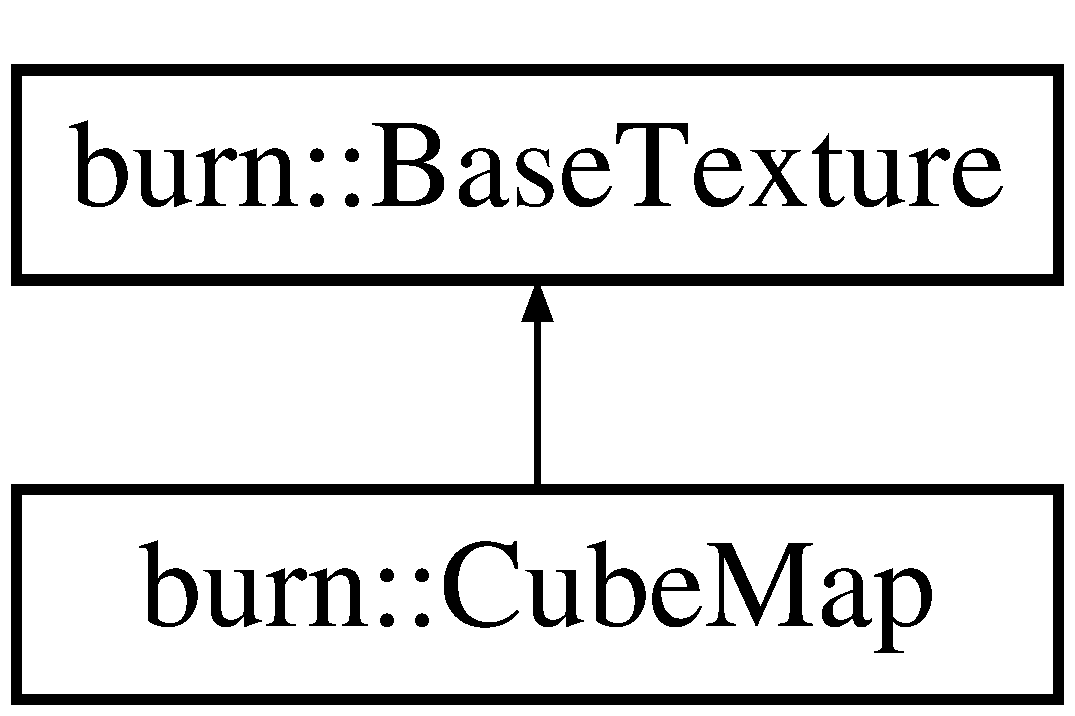
\includegraphics[height=2.000000cm]{classburn_1_1_cube_map}
\end{center}
\end{figure}
\subsection*{Public Member Functions}
\begin{DoxyCompactItemize}
\item 
\hyperlink{classburn_1_1_cube_map_ad939f4da21b13dc151b40fc00f0c9190}{Cube\-Map} ()
\item 
\hyperlink{classburn_1_1_cube_map_a598b2f65a23c9e5f6953674e4ecf0ef2}{Cube\-Map} (const \hyperlink{classburn_1_1_cube_map}{Cube\-Map} \&other)
\item 
\hyperlink{classburn_1_1_cube_map}{Cube\-Map} \& \hyperlink{classburn_1_1_cube_map_a8d69eda5fbff34f7546fe4c5b492cb5e}{operator=} (const \hyperlink{classburn_1_1_cube_map}{Cube\-Map} \&other)
\item 
\hyperlink{classburn_1_1_cube_map_a2e4355a56bbfd2ce2e3ee7b8dbff3dee}{$\sim$\-Cube\-Map} ()
\item 
bool \hyperlink{classburn_1_1_cube_map_aadf42f29ffdb3ae94cda581f55ac6f72}{load\-From\-File} (const std\-::string \&file\-Positive\-X, const std\-::string \&file\-Negative\-X, const std\-::string \&file\-Positive\-Y, const std\-::string \&file\-Negative\-Y, const std\-::string \&file\-Positive\-Z, const std\-::string \&file\-Negative\-Z)
\item 
bool \hyperlink{classburn_1_1_cube_map_a34570ba1966f5267f074a5e967bdefaa}{is\-Created} () const 
\end{DoxyCompactItemize}
\subsection*{Additional Inherited Members}


\subsection{Constructor \& Destructor Documentation}
\hypertarget{classburn_1_1_cube_map_ad939f4da21b13dc151b40fc00f0c9190}{\index{burn\-::\-Cube\-Map@{burn\-::\-Cube\-Map}!Cube\-Map@{Cube\-Map}}
\index{Cube\-Map@{Cube\-Map}!burn::CubeMap@{burn\-::\-Cube\-Map}}
\subsubsection[{Cube\-Map}]{\setlength{\rightskip}{0pt plus 5cm}burn\-::\-Cube\-Map\-::\-Cube\-Map (
\begin{DoxyParamCaption}
{}
\end{DoxyParamCaption}
)}}\label{classburn_1_1_cube_map_ad939f4da21b13dc151b40fc00f0c9190}
\hypertarget{classburn_1_1_cube_map_a598b2f65a23c9e5f6953674e4ecf0ef2}{\index{burn\-::\-Cube\-Map@{burn\-::\-Cube\-Map}!Cube\-Map@{Cube\-Map}}
\index{Cube\-Map@{Cube\-Map}!burn::CubeMap@{burn\-::\-Cube\-Map}}
\subsubsection[{Cube\-Map}]{\setlength{\rightskip}{0pt plus 5cm}burn\-::\-Cube\-Map\-::\-Cube\-Map (
\begin{DoxyParamCaption}
\item[{const {\bf Cube\-Map} \&}]{other}
\end{DoxyParamCaption}
)}}\label{classburn_1_1_cube_map_a598b2f65a23c9e5f6953674e4ecf0ef2}
\hypertarget{classburn_1_1_cube_map_a2e4355a56bbfd2ce2e3ee7b8dbff3dee}{\index{burn\-::\-Cube\-Map@{burn\-::\-Cube\-Map}!$\sim$\-Cube\-Map@{$\sim$\-Cube\-Map}}
\index{$\sim$\-Cube\-Map@{$\sim$\-Cube\-Map}!burn::CubeMap@{burn\-::\-Cube\-Map}}
\subsubsection[{$\sim$\-Cube\-Map}]{\setlength{\rightskip}{0pt plus 5cm}burn\-::\-Cube\-Map\-::$\sim$\-Cube\-Map (
\begin{DoxyParamCaption}
{}
\end{DoxyParamCaption}
)}}\label{classburn_1_1_cube_map_a2e4355a56bbfd2ce2e3ee7b8dbff3dee}


\subsection{Member Function Documentation}
\hypertarget{classburn_1_1_cube_map_a34570ba1966f5267f074a5e967bdefaa}{\index{burn\-::\-Cube\-Map@{burn\-::\-Cube\-Map}!is\-Created@{is\-Created}}
\index{is\-Created@{is\-Created}!burn::CubeMap@{burn\-::\-Cube\-Map}}
\subsubsection[{is\-Created}]{\setlength{\rightskip}{0pt plus 5cm}bool burn\-::\-Cube\-Map\-::is\-Created (
\begin{DoxyParamCaption}
{}
\end{DoxyParamCaption}
) const}}\label{classburn_1_1_cube_map_a34570ba1966f5267f074a5e967bdefaa}
\hypertarget{classburn_1_1_cube_map_aadf42f29ffdb3ae94cda581f55ac6f72}{\index{burn\-::\-Cube\-Map@{burn\-::\-Cube\-Map}!load\-From\-File@{load\-From\-File}}
\index{load\-From\-File@{load\-From\-File}!burn::CubeMap@{burn\-::\-Cube\-Map}}
\subsubsection[{load\-From\-File}]{\setlength{\rightskip}{0pt plus 5cm}bool burn\-::\-Cube\-Map\-::load\-From\-File (
\begin{DoxyParamCaption}
\item[{const std\-::string \&}]{file\-Positive\-X, }
\item[{const std\-::string \&}]{file\-Negative\-X, }
\item[{const std\-::string \&}]{file\-Positive\-Y, }
\item[{const std\-::string \&}]{file\-Negative\-Y, }
\item[{const std\-::string \&}]{file\-Positive\-Z, }
\item[{const std\-::string \&}]{file\-Negative\-Z}
\end{DoxyParamCaption}
)}}\label{classburn_1_1_cube_map_aadf42f29ffdb3ae94cda581f55ac6f72}
\hypertarget{classburn_1_1_cube_map_a8d69eda5fbff34f7546fe4c5b492cb5e}{\index{burn\-::\-Cube\-Map@{burn\-::\-Cube\-Map}!operator=@{operator=}}
\index{operator=@{operator=}!burn::CubeMap@{burn\-::\-Cube\-Map}}
\subsubsection[{operator=}]{\setlength{\rightskip}{0pt plus 5cm}{\bf Cube\-Map}\& burn\-::\-Cube\-Map\-::operator= (
\begin{DoxyParamCaption}
\item[{const {\bf Cube\-Map} \&}]{other}
\end{DoxyParamCaption}
)}}\label{classburn_1_1_cube_map_a8d69eda5fbff34f7546fe4c5b492cb5e}


The documentation for this class was generated from the following file\-:\begin{DoxyCompactItemize}
\item 
include/\-Burngine/\-Graphics/\-Texture/\hyperlink{_cube_map_8h}{Cube\-Map.\-h}\end{DoxyCompactItemize}

\hypertarget{classburn_1_1_directional_light}{\section{burn\-:\-:Directional\-Light Class Reference}
\label{classburn_1_1_directional_light}\index{burn\-::\-Directional\-Light@{burn\-::\-Directional\-Light}}
}


{\ttfamily \#include $<$Directional\-Light.\-h$>$}

Inheritance diagram for burn\-:\-:Directional\-Light\-:\begin{figure}[H]
\begin{center}
\leavevmode
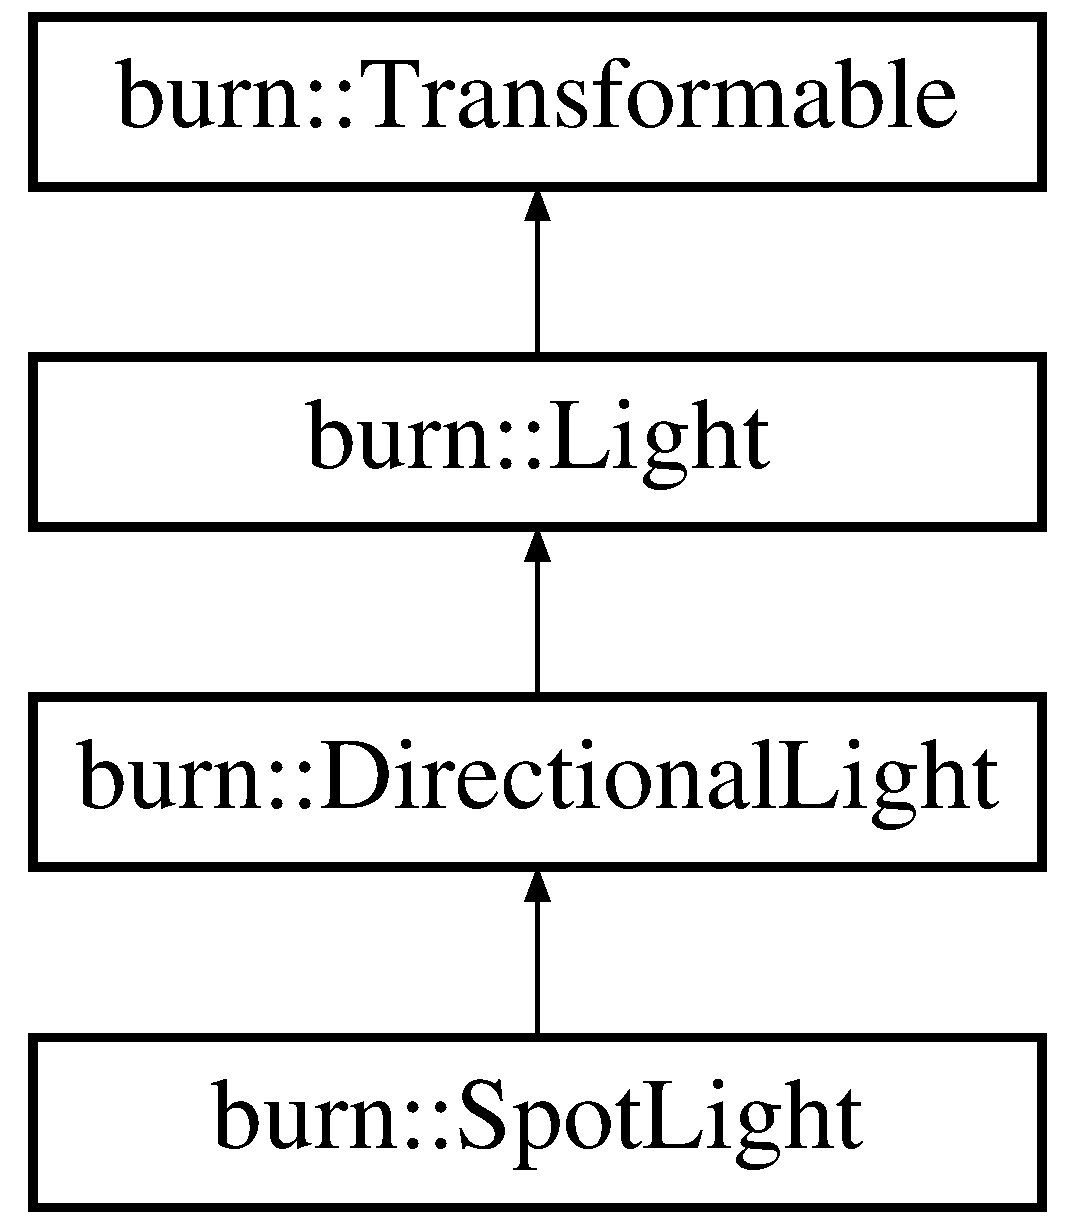
\includegraphics[height=4.000000cm]{classburn_1_1_directional_light}
\end{center}
\end{figure}
\subsection*{Public Member Functions}
\begin{DoxyCompactItemize}
\item 
\hyperlink{classburn_1_1_directional_light_ae3c3bf4a5e7ff1c9d3bf3483216f181c}{Directional\-Light} ()
\item 
\hyperlink{namespaceburn_a58a411b9d83c7970518a9250c1c78068}{Vector4f} \hyperlink{classburn_1_1_directional_light_a3035e2fc3eb45cb08166bec909237ae5}{get\-Direction} () const 
\item 
void \hyperlink{classburn_1_1_directional_light_a33e0b0f6d4cc8c236bf3a690b8e7f356}{bind\-Shadow\-Map} () const 
\item 
virtual void \hyperlink{classburn_1_1_directional_light_a84eb0090ded76e9f73d351ff87a54795}{update\-Shadow\-Map} (const std\-::vector$<$ \hyperlink{classburn_1_1_scene_node}{Scene\-Node} $\ast$ $>$ \&nodes)
\end{DoxyCompactItemize}
\subsection*{Protected Attributes}
\begin{DoxyCompactItemize}
\item 
\hyperlink{classburn_1_1_shadow_map}{Shadow\-Map} \hyperlink{classburn_1_1_directional_light_acbeffa715a9e27537c7521e0218330ff}{\-\_\-shadow\-Map}
\end{DoxyCompactItemize}
\subsection*{Additional Inherited Members}


\subsection{Constructor \& Destructor Documentation}
\hypertarget{classburn_1_1_directional_light_ae3c3bf4a5e7ff1c9d3bf3483216f181c}{\index{burn\-::\-Directional\-Light@{burn\-::\-Directional\-Light}!Directional\-Light@{Directional\-Light}}
\index{Directional\-Light@{Directional\-Light}!burn::DirectionalLight@{burn\-::\-Directional\-Light}}
\subsubsection[{Directional\-Light}]{\setlength{\rightskip}{0pt plus 5cm}burn\-::\-Directional\-Light\-::\-Directional\-Light (
\begin{DoxyParamCaption}
{}
\end{DoxyParamCaption}
)}}\label{classburn_1_1_directional_light_ae3c3bf4a5e7ff1c9d3bf3483216f181c}


\subsection{Member Function Documentation}
\hypertarget{classburn_1_1_directional_light_a33e0b0f6d4cc8c236bf3a690b8e7f356}{\index{burn\-::\-Directional\-Light@{burn\-::\-Directional\-Light}!bind\-Shadow\-Map@{bind\-Shadow\-Map}}
\index{bind\-Shadow\-Map@{bind\-Shadow\-Map}!burn::DirectionalLight@{burn\-::\-Directional\-Light}}
\subsubsection[{bind\-Shadow\-Map}]{\setlength{\rightskip}{0pt plus 5cm}void burn\-::\-Directional\-Light\-::bind\-Shadow\-Map (
\begin{DoxyParamCaption}
{}
\end{DoxyParamCaption}
) const}}\label{classburn_1_1_directional_light_a33e0b0f6d4cc8c236bf3a690b8e7f356}
\hypertarget{classburn_1_1_directional_light_a3035e2fc3eb45cb08166bec909237ae5}{\index{burn\-::\-Directional\-Light@{burn\-::\-Directional\-Light}!get\-Direction@{get\-Direction}}
\index{get\-Direction@{get\-Direction}!burn::DirectionalLight@{burn\-::\-Directional\-Light}}
\subsubsection[{get\-Direction}]{\setlength{\rightskip}{0pt plus 5cm}{\bf Vector4f} burn\-::\-Directional\-Light\-::get\-Direction (
\begin{DoxyParamCaption}
{}
\end{DoxyParamCaption}
) const}}\label{classburn_1_1_directional_light_a3035e2fc3eb45cb08166bec909237ae5}
\hypertarget{classburn_1_1_directional_light_a84eb0090ded76e9f73d351ff87a54795}{\index{burn\-::\-Directional\-Light@{burn\-::\-Directional\-Light}!update\-Shadow\-Map@{update\-Shadow\-Map}}
\index{update\-Shadow\-Map@{update\-Shadow\-Map}!burn::DirectionalLight@{burn\-::\-Directional\-Light}}
\subsubsection[{update\-Shadow\-Map}]{\setlength{\rightskip}{0pt plus 5cm}virtual void burn\-::\-Directional\-Light\-::update\-Shadow\-Map (
\begin{DoxyParamCaption}
\item[{const std\-::vector$<$ {\bf Scene\-Node} $\ast$ $>$ \&}]{nodes}
\end{DoxyParamCaption}
)\hspace{0.3cm}{\ttfamily [virtual]}}}\label{classburn_1_1_directional_light_a84eb0090ded76e9f73d351ff87a54795}


Reimplemented from \hyperlink{classburn_1_1_light_af14d6771a1b6ff04195467f5c1c6a312}{burn\-::\-Light}.



Reimplemented in \hyperlink{classburn_1_1_spot_light_ab16ad5f4da0fe8fc9cdd07b2931259ee}{burn\-::\-Spot\-Light}.



\subsection{Member Data Documentation}
\hypertarget{classburn_1_1_directional_light_acbeffa715a9e27537c7521e0218330ff}{\index{burn\-::\-Directional\-Light@{burn\-::\-Directional\-Light}!\-\_\-shadow\-Map@{\-\_\-shadow\-Map}}
\index{\-\_\-shadow\-Map@{\-\_\-shadow\-Map}!burn::DirectionalLight@{burn\-::\-Directional\-Light}}
\subsubsection[{\-\_\-shadow\-Map}]{\setlength{\rightskip}{0pt plus 5cm}{\bf Shadow\-Map} burn\-::\-Directional\-Light\-::\-\_\-shadow\-Map\hspace{0.3cm}{\ttfamily [protected]}}}\label{classburn_1_1_directional_light_acbeffa715a9e27537c7521e0218330ff}


The documentation for this class was generated from the following file\-:\begin{DoxyCompactItemize}
\item 
include/\-Burngine/\-Graphics/\-Scene/\hyperlink{_directional_light_8h}{Directional\-Light.\-h}\end{DoxyCompactItemize}

\hypertarget{classburn_1_1_font}{\section{burn\-:\-:Font Class Reference}
\label{classburn_1_1_font}\index{burn\-::\-Font@{burn\-::\-Font}}
}


{\ttfamily \#include $<$Font.\-h$>$}

\subsection*{Public Member Functions}
\begin{DoxyCompactItemize}
\item 
\hyperlink{classburn_1_1_font_a5e89a49100bd01b72b95ad26c869a4c8}{Font} ()
\item 
\hyperlink{classburn_1_1_font_adbdef3544e8d1925de8b1305e1e990d3}{$\sim$\-Font} ()
\item 
bool \hyperlink{classburn_1_1_font_a0788de2b9685bd41482124efada486f3}{load\-From\-File} (const std\-::string \&file)
\item 
const \hyperlink{classburn_1_1_character}{Character} \& \hyperlink{classburn_1_1_font_a25b92e02bf9a20eb1c78ba415c14c765}{get\-Character} (const \hyperlink{namespaceburn_ab40b09022209bd449d317c1f0e95356b}{Uint32} \&code\-Point, const unsigned int \&font\-Size)
\item 
bool \hyperlink{classburn_1_1_font_a46ffb674f4f8f3245feccda520750e8e}{is\-Loaded} () const 
\item 
float \hyperlink{classburn_1_1_font_a779fa753f88cb28668ab143ec313e7d0}{get\-Next\-Line\-Offset} () const 
\item 
float \hyperlink{classburn_1_1_font_abea302cec9ab9610328e5b43d7b188c7}{get\-Space\-Offset} () const 
\end{DoxyCompactItemize}


\subsection{Constructor \& Destructor Documentation}
\hypertarget{classburn_1_1_font_a5e89a49100bd01b72b95ad26c869a4c8}{\index{burn\-::\-Font@{burn\-::\-Font}!Font@{Font}}
\index{Font@{Font}!burn::Font@{burn\-::\-Font}}
\subsubsection[{Font}]{\setlength{\rightskip}{0pt plus 5cm}burn\-::\-Font\-::\-Font (
\begin{DoxyParamCaption}
{}
\end{DoxyParamCaption}
)}}\label{classburn_1_1_font_a5e89a49100bd01b72b95ad26c869a4c8}
\hypertarget{classburn_1_1_font_adbdef3544e8d1925de8b1305e1e990d3}{\index{burn\-::\-Font@{burn\-::\-Font}!$\sim$\-Font@{$\sim$\-Font}}
\index{$\sim$\-Font@{$\sim$\-Font}!burn::Font@{burn\-::\-Font}}
\subsubsection[{$\sim$\-Font}]{\setlength{\rightskip}{0pt plus 5cm}burn\-::\-Font\-::$\sim$\-Font (
\begin{DoxyParamCaption}
{}
\end{DoxyParamCaption}
)}}\label{classburn_1_1_font_adbdef3544e8d1925de8b1305e1e990d3}


\subsection{Member Function Documentation}
\hypertarget{classburn_1_1_font_a25b92e02bf9a20eb1c78ba415c14c765}{\index{burn\-::\-Font@{burn\-::\-Font}!get\-Character@{get\-Character}}
\index{get\-Character@{get\-Character}!burn::Font@{burn\-::\-Font}}
\subsubsection[{get\-Character}]{\setlength{\rightskip}{0pt plus 5cm}const {\bf Character}\& burn\-::\-Font\-::get\-Character (
\begin{DoxyParamCaption}
\item[{const {\bf Uint32} \&}]{code\-Point, }
\item[{const unsigned int \&}]{font\-Size}
\end{DoxyParamCaption}
)}}\label{classburn_1_1_font_a25b92e02bf9a20eb1c78ba415c14c765}
\hypertarget{classburn_1_1_font_a779fa753f88cb28668ab143ec313e7d0}{\index{burn\-::\-Font@{burn\-::\-Font}!get\-Next\-Line\-Offset@{get\-Next\-Line\-Offset}}
\index{get\-Next\-Line\-Offset@{get\-Next\-Line\-Offset}!burn::Font@{burn\-::\-Font}}
\subsubsection[{get\-Next\-Line\-Offset}]{\setlength{\rightskip}{0pt plus 5cm}float burn\-::\-Font\-::get\-Next\-Line\-Offset (
\begin{DoxyParamCaption}
{}
\end{DoxyParamCaption}
) const}}\label{classburn_1_1_font_a779fa753f88cb28668ab143ec313e7d0}
\hypertarget{classburn_1_1_font_abea302cec9ab9610328e5b43d7b188c7}{\index{burn\-::\-Font@{burn\-::\-Font}!get\-Space\-Offset@{get\-Space\-Offset}}
\index{get\-Space\-Offset@{get\-Space\-Offset}!burn::Font@{burn\-::\-Font}}
\subsubsection[{get\-Space\-Offset}]{\setlength{\rightskip}{0pt plus 5cm}float burn\-::\-Font\-::get\-Space\-Offset (
\begin{DoxyParamCaption}
{}
\end{DoxyParamCaption}
) const}}\label{classburn_1_1_font_abea302cec9ab9610328e5b43d7b188c7}
\hypertarget{classburn_1_1_font_a46ffb674f4f8f3245feccda520750e8e}{\index{burn\-::\-Font@{burn\-::\-Font}!is\-Loaded@{is\-Loaded}}
\index{is\-Loaded@{is\-Loaded}!burn::Font@{burn\-::\-Font}}
\subsubsection[{is\-Loaded}]{\setlength{\rightskip}{0pt plus 5cm}bool burn\-::\-Font\-::is\-Loaded (
\begin{DoxyParamCaption}
{}
\end{DoxyParamCaption}
) const}}\label{classburn_1_1_font_a46ffb674f4f8f3245feccda520750e8e}
\hypertarget{classburn_1_1_font_a0788de2b9685bd41482124efada486f3}{\index{burn\-::\-Font@{burn\-::\-Font}!load\-From\-File@{load\-From\-File}}
\index{load\-From\-File@{load\-From\-File}!burn::Font@{burn\-::\-Font}}
\subsubsection[{load\-From\-File}]{\setlength{\rightskip}{0pt plus 5cm}bool burn\-::\-Font\-::load\-From\-File (
\begin{DoxyParamCaption}
\item[{const std\-::string \&}]{file}
\end{DoxyParamCaption}
)}}\label{classburn_1_1_font_a0788de2b9685bd41482124efada486f3}


The documentation for this class was generated from the following file\-:\begin{DoxyCompactItemize}
\item 
include/\-Burngine/\-Graphics/\-Gui/\hyperlink{_font_8h}{Font.\-h}\end{DoxyCompactItemize}

\hypertarget{classburn_1_1_gui}{\section{burn\-:\-:Gui Class Reference}
\label{classburn_1_1_gui}\index{burn\-::\-Gui@{burn\-::\-Gui}}
}


{\ttfamily \#include $<$Gui.\-h$>$}

\subsection*{Public Member Functions}
\begin{DoxyCompactItemize}
\item 
\hyperlink{classburn_1_1_gui_a3f4ea23725b735438f1897b40b98036d}{Gui} ()
\item 
\hyperlink{classburn_1_1_gui_a57f216f38585ce367c5821bec2a57f1b}{$\sim$\-Gui} ()
\item 
void \hyperlink{classburn_1_1_gui_a1e1a4b3d6dd025ea46603fe665c337a1}{attach\-Node} (\hyperlink{classburn_1_1_gui_node}{Gui\-Node} \&node)
\item 
void \hyperlink{classburn_1_1_gui_ad2e7ed75e7c984b1f0e623f200193bba}{detach\-Node} (\hyperlink{classburn_1_1_gui_node}{Gui\-Node} \&node)
\item 
void \hyperlink{classburn_1_1_gui_a0be74e62349e2cf561c4a29a7fc857f9}{detach\-All} ()
\item 
void \hyperlink{classburn_1_1_gui_aaa88372f63b7c0f4e8beecca3af11021}{draw} ()
\item 
void \hyperlink{classburn_1_1_gui_a13e986deced164330db42a6e408e6b4b}{sort\-Nodes} ()
\end{DoxyCompactItemize}


\subsection{Constructor \& Destructor Documentation}
\hypertarget{classburn_1_1_gui_a3f4ea23725b735438f1897b40b98036d}{\index{burn\-::\-Gui@{burn\-::\-Gui}!Gui@{Gui}}
\index{Gui@{Gui}!burn::Gui@{burn\-::\-Gui}}
\subsubsection[{Gui}]{\setlength{\rightskip}{0pt plus 5cm}burn\-::\-Gui\-::\-Gui (
\begin{DoxyParamCaption}
{}
\end{DoxyParamCaption}
)}}\label{classburn_1_1_gui_a3f4ea23725b735438f1897b40b98036d}
\hypertarget{classburn_1_1_gui_a57f216f38585ce367c5821bec2a57f1b}{\index{burn\-::\-Gui@{burn\-::\-Gui}!$\sim$\-Gui@{$\sim$\-Gui}}
\index{$\sim$\-Gui@{$\sim$\-Gui}!burn::Gui@{burn\-::\-Gui}}
\subsubsection[{$\sim$\-Gui}]{\setlength{\rightskip}{0pt plus 5cm}burn\-::\-Gui\-::$\sim$\-Gui (
\begin{DoxyParamCaption}
{}
\end{DoxyParamCaption}
)}}\label{classburn_1_1_gui_a57f216f38585ce367c5821bec2a57f1b}


\subsection{Member Function Documentation}
\hypertarget{classburn_1_1_gui_a1e1a4b3d6dd025ea46603fe665c337a1}{\index{burn\-::\-Gui@{burn\-::\-Gui}!attach\-Node@{attach\-Node}}
\index{attach\-Node@{attach\-Node}!burn::Gui@{burn\-::\-Gui}}
\subsubsection[{attach\-Node}]{\setlength{\rightskip}{0pt plus 5cm}void burn\-::\-Gui\-::attach\-Node (
\begin{DoxyParamCaption}
\item[{{\bf Gui\-Node} \&}]{node}
\end{DoxyParamCaption}
)}}\label{classburn_1_1_gui_a1e1a4b3d6dd025ea46603fe665c337a1}
\hypertarget{classburn_1_1_gui_a0be74e62349e2cf561c4a29a7fc857f9}{\index{burn\-::\-Gui@{burn\-::\-Gui}!detach\-All@{detach\-All}}
\index{detach\-All@{detach\-All}!burn::Gui@{burn\-::\-Gui}}
\subsubsection[{detach\-All}]{\setlength{\rightskip}{0pt plus 5cm}void burn\-::\-Gui\-::detach\-All (
\begin{DoxyParamCaption}
{}
\end{DoxyParamCaption}
)}}\label{classburn_1_1_gui_a0be74e62349e2cf561c4a29a7fc857f9}
\hypertarget{classburn_1_1_gui_ad2e7ed75e7c984b1f0e623f200193bba}{\index{burn\-::\-Gui@{burn\-::\-Gui}!detach\-Node@{detach\-Node}}
\index{detach\-Node@{detach\-Node}!burn::Gui@{burn\-::\-Gui}}
\subsubsection[{detach\-Node}]{\setlength{\rightskip}{0pt plus 5cm}void burn\-::\-Gui\-::detach\-Node (
\begin{DoxyParamCaption}
\item[{{\bf Gui\-Node} \&}]{node}
\end{DoxyParamCaption}
)}}\label{classburn_1_1_gui_ad2e7ed75e7c984b1f0e623f200193bba}
\hypertarget{classburn_1_1_gui_aaa88372f63b7c0f4e8beecca3af11021}{\index{burn\-::\-Gui@{burn\-::\-Gui}!draw@{draw}}
\index{draw@{draw}!burn::Gui@{burn\-::\-Gui}}
\subsubsection[{draw}]{\setlength{\rightskip}{0pt plus 5cm}void burn\-::\-Gui\-::draw (
\begin{DoxyParamCaption}
{}
\end{DoxyParamCaption}
)}}\label{classburn_1_1_gui_aaa88372f63b7c0f4e8beecca3af11021}
\hypertarget{classburn_1_1_gui_a13e986deced164330db42a6e408e6b4b}{\index{burn\-::\-Gui@{burn\-::\-Gui}!sort\-Nodes@{sort\-Nodes}}
\index{sort\-Nodes@{sort\-Nodes}!burn::Gui@{burn\-::\-Gui}}
\subsubsection[{sort\-Nodes}]{\setlength{\rightskip}{0pt plus 5cm}void burn\-::\-Gui\-::sort\-Nodes (
\begin{DoxyParamCaption}
{}
\end{DoxyParamCaption}
)}}\label{classburn_1_1_gui_a13e986deced164330db42a6e408e6b4b}


The documentation for this class was generated from the following file\-:\begin{DoxyCompactItemize}
\item 
include/\-Burngine/\-Graphics/\-Gui/\hyperlink{_gui_8h}{Gui.\-h}\end{DoxyCompactItemize}

\hypertarget{classburn_1_1_gui_node}{\section{burn\-:\-:Gui\-Node Class Reference}
\label{classburn_1_1_gui_node}\index{burn\-::\-Gui\-Node@{burn\-::\-Gui\-Node}}
}


{\ttfamily \#include $<$Gui\-Node.\-h$>$}

Inheritance diagram for burn\-:\-:Gui\-Node\-:\begin{figure}[H]
\begin{center}
\leavevmode
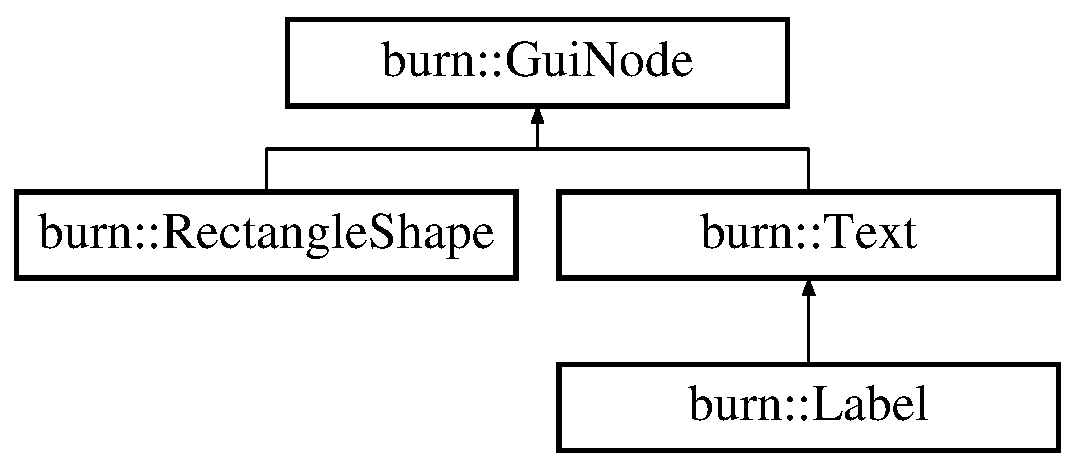
\includegraphics[height=3.000000cm]{classburn_1_1_gui_node}
\end{center}
\end{figure}
\subsection*{Public Member Functions}
\begin{DoxyCompactItemize}
\item 
\hyperlink{classburn_1_1_gui_node_ae908f29b71dda5ea724c742cfda3cd2a}{Gui\-Node} ()
\item 
virtual \hyperlink{classburn_1_1_gui_node_a5c047d11bef782a5261ce24d946612a8}{$\sim$\-Gui\-Node} ()
\item 
virtual void \hyperlink{classburn_1_1_gui_node_ac283552733ae59c4f1b7fa05c79cb517}{draw} ()=0
\item 
void \hyperlink{classburn_1_1_gui_node_a75f542965a10945fa2894a722def8337}{set\-Position} (const \hyperlink{namespaceburn_af5ed9eb70cbf0fb572098ff43e146a0a}{Vector2f} \&position)
\item 
const \hyperlink{namespaceburn_af5ed9eb70cbf0fb572098ff43e146a0a}{Vector2f} \& \hyperlink{classburn_1_1_gui_node_af3ddf018a01e587d110d44c16baa5ae8}{get\-Position} () const 
\item 
void \hyperlink{classburn_1_1_gui_node_aa02ac7225479a0a5652b6b759ba66dc7}{set\-Rotation} (const float \&rotation)
\item 
const float \& \hyperlink{classburn_1_1_gui_node_acc490b42584e6008b828a4251a88600a}{get\-Rotation} () const 
\item 
void \hyperlink{classburn_1_1_gui_node_a780a3f0e7fc21e5ab98f01e4bd5d87a3}{rotate} (const float \&angle)
\item 
void \hyperlink{classburn_1_1_gui_node_a4ad80df2dd7319d5ad7c036369ddf95b}{move} (const \hyperlink{namespaceburn_af5ed9eb70cbf0fb572098ff43e146a0a}{Vector2f} \&offset)
\item 
void \hyperlink{classburn_1_1_gui_node_a8e75af236c12312492e06242b8b58c13}{move} (const float \&offset\-X, const float \&offset\-Y)
\item 
void \hyperlink{classburn_1_1_gui_node_a12fdf6059b778dfbdc8737befcf09018}{set\-Z\-Index} (const \hyperlink{namespaceburn_a96c2e82d6da686c64a6f330628466b05}{Int32} \&z\-Index)
\item 
const \hyperlink{namespaceburn_a96c2e82d6da686c64a6f330628466b05}{Int32} \& \hyperlink{classburn_1_1_gui_node_a6d12929d442ae3e2a92704dfe9a26c12}{get\-Z\-Index} () const 
\item 
void \hyperlink{classburn_1_1_gui_node_a7636e6452ab00f08bfbc0841fb843788}{add\-Parent\-Gui} (\hyperlink{classburn_1_1_gui}{Gui} $\ast$parent)
\item 
void \hyperlink{classburn_1_1_gui_node_ad67e018354a2c81d64658aece6efb7c3}{remove\-Parent\-Gui} (\hyperlink{classburn_1_1_gui}{Gui} $\ast$parent)
\end{DoxyCompactItemize}
\subsection*{Protected Attributes}
\begin{DoxyCompactItemize}
\item 
\hyperlink{namespaceburn_af5ed9eb70cbf0fb572098ff43e146a0a}{Vector2f} \hyperlink{classburn_1_1_gui_node_a3047fb0cd29eb1cbc1a4ca5569b3d1bb}{\-\_\-position}
\item 
float \hyperlink{classburn_1_1_gui_node_aee62a004027766c6e7fd8947f150e759}{\-\_\-rotation}
\item 
\hyperlink{namespaceburn_a96c2e82d6da686c64a6f330628466b05}{Int32} \hyperlink{classburn_1_1_gui_node_a0ff802eeb35c2c27b9850cbd59449923}{\-\_\-z\-Index}
\item 
std\-::vector$<$ \hyperlink{classburn_1_1_gui}{Gui} $\ast$ $>$ \hyperlink{classburn_1_1_gui_node_af37b701f475d8046a3f864df6e39faf4}{\-\_\-parents}
\end{DoxyCompactItemize}


\subsection{Constructor \& Destructor Documentation}
\hypertarget{classburn_1_1_gui_node_ae908f29b71dda5ea724c742cfda3cd2a}{\index{burn\-::\-Gui\-Node@{burn\-::\-Gui\-Node}!Gui\-Node@{Gui\-Node}}
\index{Gui\-Node@{Gui\-Node}!burn::GuiNode@{burn\-::\-Gui\-Node}}
\subsubsection[{Gui\-Node}]{\setlength{\rightskip}{0pt plus 5cm}burn\-::\-Gui\-Node\-::\-Gui\-Node (
\begin{DoxyParamCaption}
{}
\end{DoxyParamCaption}
)}}\label{classburn_1_1_gui_node_ae908f29b71dda5ea724c742cfda3cd2a}
\hypertarget{classburn_1_1_gui_node_a5c047d11bef782a5261ce24d946612a8}{\index{burn\-::\-Gui\-Node@{burn\-::\-Gui\-Node}!$\sim$\-Gui\-Node@{$\sim$\-Gui\-Node}}
\index{$\sim$\-Gui\-Node@{$\sim$\-Gui\-Node}!burn::GuiNode@{burn\-::\-Gui\-Node}}
\subsubsection[{$\sim$\-Gui\-Node}]{\setlength{\rightskip}{0pt plus 5cm}virtual burn\-::\-Gui\-Node\-::$\sim$\-Gui\-Node (
\begin{DoxyParamCaption}
{}
\end{DoxyParamCaption}
)\hspace{0.3cm}{\ttfamily [virtual]}}}\label{classburn_1_1_gui_node_a5c047d11bef782a5261ce24d946612a8}


\subsection{Member Function Documentation}
\hypertarget{classburn_1_1_gui_node_a7636e6452ab00f08bfbc0841fb843788}{\index{burn\-::\-Gui\-Node@{burn\-::\-Gui\-Node}!add\-Parent\-Gui@{add\-Parent\-Gui}}
\index{add\-Parent\-Gui@{add\-Parent\-Gui}!burn::GuiNode@{burn\-::\-Gui\-Node}}
\subsubsection[{add\-Parent\-Gui}]{\setlength{\rightskip}{0pt plus 5cm}void burn\-::\-Gui\-Node\-::add\-Parent\-Gui (
\begin{DoxyParamCaption}
\item[{{\bf Gui} $\ast$}]{parent}
\end{DoxyParamCaption}
)}}\label{classburn_1_1_gui_node_a7636e6452ab00f08bfbc0841fb843788}
\hypertarget{classburn_1_1_gui_node_ac283552733ae59c4f1b7fa05c79cb517}{\index{burn\-::\-Gui\-Node@{burn\-::\-Gui\-Node}!draw@{draw}}
\index{draw@{draw}!burn::GuiNode@{burn\-::\-Gui\-Node}}
\subsubsection[{draw}]{\setlength{\rightskip}{0pt plus 5cm}virtual void burn\-::\-Gui\-Node\-::draw (
\begin{DoxyParamCaption}
{}
\end{DoxyParamCaption}
)\hspace{0.3cm}{\ttfamily [pure virtual]}}}\label{classburn_1_1_gui_node_ac283552733ae59c4f1b7fa05c79cb517}


Implemented in \hyperlink{classburn_1_1_text_aa451ad17d21dc9c12cef712aa41914bf}{burn\-::\-Text}, \hyperlink{classburn_1_1_rectangle_shape_a39c5c1e57ada4a6beb32a84a501baabf}{burn\-::\-Rectangle\-Shape}, and \hyperlink{classburn_1_1_label_a23eaa7ccb0a68e6691a89133cb4254d5}{burn\-::\-Label}.

\hypertarget{classburn_1_1_gui_node_af3ddf018a01e587d110d44c16baa5ae8}{\index{burn\-::\-Gui\-Node@{burn\-::\-Gui\-Node}!get\-Position@{get\-Position}}
\index{get\-Position@{get\-Position}!burn::GuiNode@{burn\-::\-Gui\-Node}}
\subsubsection[{get\-Position}]{\setlength{\rightskip}{0pt plus 5cm}const {\bf Vector2f}\& burn\-::\-Gui\-Node\-::get\-Position (
\begin{DoxyParamCaption}
{}
\end{DoxyParamCaption}
) const}}\label{classburn_1_1_gui_node_af3ddf018a01e587d110d44c16baa5ae8}
\hypertarget{classburn_1_1_gui_node_acc490b42584e6008b828a4251a88600a}{\index{burn\-::\-Gui\-Node@{burn\-::\-Gui\-Node}!get\-Rotation@{get\-Rotation}}
\index{get\-Rotation@{get\-Rotation}!burn::GuiNode@{burn\-::\-Gui\-Node}}
\subsubsection[{get\-Rotation}]{\setlength{\rightskip}{0pt plus 5cm}const float\& burn\-::\-Gui\-Node\-::get\-Rotation (
\begin{DoxyParamCaption}
{}
\end{DoxyParamCaption}
) const}}\label{classburn_1_1_gui_node_acc490b42584e6008b828a4251a88600a}
\hypertarget{classburn_1_1_gui_node_a6d12929d442ae3e2a92704dfe9a26c12}{\index{burn\-::\-Gui\-Node@{burn\-::\-Gui\-Node}!get\-Z\-Index@{get\-Z\-Index}}
\index{get\-Z\-Index@{get\-Z\-Index}!burn::GuiNode@{burn\-::\-Gui\-Node}}
\subsubsection[{get\-Z\-Index}]{\setlength{\rightskip}{0pt plus 5cm}const {\bf Int32}\& burn\-::\-Gui\-Node\-::get\-Z\-Index (
\begin{DoxyParamCaption}
{}
\end{DoxyParamCaption}
) const}}\label{classburn_1_1_gui_node_a6d12929d442ae3e2a92704dfe9a26c12}
\hypertarget{classburn_1_1_gui_node_a4ad80df2dd7319d5ad7c036369ddf95b}{\index{burn\-::\-Gui\-Node@{burn\-::\-Gui\-Node}!move@{move}}
\index{move@{move}!burn::GuiNode@{burn\-::\-Gui\-Node}}
\subsubsection[{move}]{\setlength{\rightskip}{0pt plus 5cm}void burn\-::\-Gui\-Node\-::move (
\begin{DoxyParamCaption}
\item[{const {\bf Vector2f} \&}]{offset}
\end{DoxyParamCaption}
)}}\label{classburn_1_1_gui_node_a4ad80df2dd7319d5ad7c036369ddf95b}
\hypertarget{classburn_1_1_gui_node_a8e75af236c12312492e06242b8b58c13}{\index{burn\-::\-Gui\-Node@{burn\-::\-Gui\-Node}!move@{move}}
\index{move@{move}!burn::GuiNode@{burn\-::\-Gui\-Node}}
\subsubsection[{move}]{\setlength{\rightskip}{0pt plus 5cm}void burn\-::\-Gui\-Node\-::move (
\begin{DoxyParamCaption}
\item[{const float \&}]{offset\-X, }
\item[{const float \&}]{offset\-Y}
\end{DoxyParamCaption}
)}}\label{classburn_1_1_gui_node_a8e75af236c12312492e06242b8b58c13}
\hypertarget{classburn_1_1_gui_node_ad67e018354a2c81d64658aece6efb7c3}{\index{burn\-::\-Gui\-Node@{burn\-::\-Gui\-Node}!remove\-Parent\-Gui@{remove\-Parent\-Gui}}
\index{remove\-Parent\-Gui@{remove\-Parent\-Gui}!burn::GuiNode@{burn\-::\-Gui\-Node}}
\subsubsection[{remove\-Parent\-Gui}]{\setlength{\rightskip}{0pt plus 5cm}void burn\-::\-Gui\-Node\-::remove\-Parent\-Gui (
\begin{DoxyParamCaption}
\item[{{\bf Gui} $\ast$}]{parent}
\end{DoxyParamCaption}
)}}\label{classburn_1_1_gui_node_ad67e018354a2c81d64658aece6efb7c3}
\hypertarget{classburn_1_1_gui_node_a780a3f0e7fc21e5ab98f01e4bd5d87a3}{\index{burn\-::\-Gui\-Node@{burn\-::\-Gui\-Node}!rotate@{rotate}}
\index{rotate@{rotate}!burn::GuiNode@{burn\-::\-Gui\-Node}}
\subsubsection[{rotate}]{\setlength{\rightskip}{0pt plus 5cm}void burn\-::\-Gui\-Node\-::rotate (
\begin{DoxyParamCaption}
\item[{const float \&}]{angle}
\end{DoxyParamCaption}
)}}\label{classburn_1_1_gui_node_a780a3f0e7fc21e5ab98f01e4bd5d87a3}
\hypertarget{classburn_1_1_gui_node_a75f542965a10945fa2894a722def8337}{\index{burn\-::\-Gui\-Node@{burn\-::\-Gui\-Node}!set\-Position@{set\-Position}}
\index{set\-Position@{set\-Position}!burn::GuiNode@{burn\-::\-Gui\-Node}}
\subsubsection[{set\-Position}]{\setlength{\rightskip}{0pt plus 5cm}void burn\-::\-Gui\-Node\-::set\-Position (
\begin{DoxyParamCaption}
\item[{const {\bf Vector2f} \&}]{position}
\end{DoxyParamCaption}
)}}\label{classburn_1_1_gui_node_a75f542965a10945fa2894a722def8337}
\hypertarget{classburn_1_1_gui_node_aa02ac7225479a0a5652b6b759ba66dc7}{\index{burn\-::\-Gui\-Node@{burn\-::\-Gui\-Node}!set\-Rotation@{set\-Rotation}}
\index{set\-Rotation@{set\-Rotation}!burn::GuiNode@{burn\-::\-Gui\-Node}}
\subsubsection[{set\-Rotation}]{\setlength{\rightskip}{0pt plus 5cm}void burn\-::\-Gui\-Node\-::set\-Rotation (
\begin{DoxyParamCaption}
\item[{const float \&}]{rotation}
\end{DoxyParamCaption}
)}}\label{classburn_1_1_gui_node_aa02ac7225479a0a5652b6b759ba66dc7}
\hypertarget{classburn_1_1_gui_node_a12fdf6059b778dfbdc8737befcf09018}{\index{burn\-::\-Gui\-Node@{burn\-::\-Gui\-Node}!set\-Z\-Index@{set\-Z\-Index}}
\index{set\-Z\-Index@{set\-Z\-Index}!burn::GuiNode@{burn\-::\-Gui\-Node}}
\subsubsection[{set\-Z\-Index}]{\setlength{\rightskip}{0pt plus 5cm}void burn\-::\-Gui\-Node\-::set\-Z\-Index (
\begin{DoxyParamCaption}
\item[{const {\bf Int32} \&}]{z\-Index}
\end{DoxyParamCaption}
)}}\label{classburn_1_1_gui_node_a12fdf6059b778dfbdc8737befcf09018}


\subsection{Member Data Documentation}
\hypertarget{classburn_1_1_gui_node_af37b701f475d8046a3f864df6e39faf4}{\index{burn\-::\-Gui\-Node@{burn\-::\-Gui\-Node}!\-\_\-parents@{\-\_\-parents}}
\index{\-\_\-parents@{\-\_\-parents}!burn::GuiNode@{burn\-::\-Gui\-Node}}
\subsubsection[{\-\_\-parents}]{\setlength{\rightskip}{0pt plus 5cm}std\-::vector$<${\bf Gui}$\ast$$>$ burn\-::\-Gui\-Node\-::\-\_\-parents\hspace{0.3cm}{\ttfamily [protected]}}}\label{classburn_1_1_gui_node_af37b701f475d8046a3f864df6e39faf4}
\hypertarget{classburn_1_1_gui_node_a3047fb0cd29eb1cbc1a4ca5569b3d1bb}{\index{burn\-::\-Gui\-Node@{burn\-::\-Gui\-Node}!\-\_\-position@{\-\_\-position}}
\index{\-\_\-position@{\-\_\-position}!burn::GuiNode@{burn\-::\-Gui\-Node}}
\subsubsection[{\-\_\-position}]{\setlength{\rightskip}{0pt plus 5cm}{\bf Vector2f} burn\-::\-Gui\-Node\-::\-\_\-position\hspace{0.3cm}{\ttfamily [protected]}}}\label{classburn_1_1_gui_node_a3047fb0cd29eb1cbc1a4ca5569b3d1bb}
\hypertarget{classburn_1_1_gui_node_aee62a004027766c6e7fd8947f150e759}{\index{burn\-::\-Gui\-Node@{burn\-::\-Gui\-Node}!\-\_\-rotation@{\-\_\-rotation}}
\index{\-\_\-rotation@{\-\_\-rotation}!burn::GuiNode@{burn\-::\-Gui\-Node}}
\subsubsection[{\-\_\-rotation}]{\setlength{\rightskip}{0pt plus 5cm}float burn\-::\-Gui\-Node\-::\-\_\-rotation\hspace{0.3cm}{\ttfamily [protected]}}}\label{classburn_1_1_gui_node_aee62a004027766c6e7fd8947f150e759}
\hypertarget{classburn_1_1_gui_node_a0ff802eeb35c2c27b9850cbd59449923}{\index{burn\-::\-Gui\-Node@{burn\-::\-Gui\-Node}!\-\_\-z\-Index@{\-\_\-z\-Index}}
\index{\-\_\-z\-Index@{\-\_\-z\-Index}!burn::GuiNode@{burn\-::\-Gui\-Node}}
\subsubsection[{\-\_\-z\-Index}]{\setlength{\rightskip}{0pt plus 5cm}{\bf Int32} burn\-::\-Gui\-Node\-::\-\_\-z\-Index\hspace{0.3cm}{\ttfamily [protected]}}}\label{classburn_1_1_gui_node_a0ff802eeb35c2c27b9850cbd59449923}


The documentation for this class was generated from the following file\-:\begin{DoxyCompactItemize}
\item 
include/\-Burngine/\-Graphics/\-Gui/\hyperlink{_gui_node_8h}{Gui\-Node.\-h}\end{DoxyCompactItemize}

\hypertarget{classburn_1_1_keyboard}{\section{burn\-:\-:Keyboard Class Reference}
\label{classburn_1_1_keyboard}\index{burn\-::\-Keyboard@{burn\-::\-Keyboard}}
}


{\ttfamily \#include $<$Keyboard.\-h$>$}

\subsection*{Public Types}
\begin{DoxyCompactItemize}
\item 
enum \hyperlink{classburn_1_1_keyboard_a2aabfebd78080f013e704415293a4533}{Key} \{ \\*
\hyperlink{classburn_1_1_keyboard_a2aabfebd78080f013e704415293a4533ac6129ac2879eaa94d6be30163b4f7877}{F1} = G\-L\-F\-W\-\_\-\-K\-E\-Y\-\_\-\-F1, 
\hyperlink{classburn_1_1_keyboard_a2aabfebd78080f013e704415293a4533a14274d0e38330812277e7f76a8196089}{F2} = G\-L\-F\-W\-\_\-\-K\-E\-Y\-\_\-\-F2, 
\hyperlink{classburn_1_1_keyboard_a2aabfebd78080f013e704415293a4533a8c874ea48c022f69ba27fbeb67dbf697}{F3} = G\-L\-F\-W\-\_\-\-K\-E\-Y\-\_\-\-F3, 
\hyperlink{classburn_1_1_keyboard_a2aabfebd78080f013e704415293a4533a90b08c831000643534febb9c890095c9}{F4} = G\-L\-F\-W\-\_\-\-K\-E\-Y\-\_\-\-F4, 
\\*
\hyperlink{classburn_1_1_keyboard_a2aabfebd78080f013e704415293a4533a7046d4dcb8608b6ab8deb839fb9ef834}{F5} = G\-L\-F\-W\-\_\-\-K\-E\-Y\-\_\-\-F5, 
\hyperlink{classburn_1_1_keyboard_a2aabfebd78080f013e704415293a4533a68905a78cb4faf1430d44957fa6b6ef8}{F6} = G\-L\-F\-W\-\_\-\-K\-E\-Y\-\_\-\-F6, 
\hyperlink{classburn_1_1_keyboard_a2aabfebd78080f013e704415293a4533ac2b32c682e7f2279dc96ab3c86912f67}{F7} = G\-L\-F\-W\-\_\-\-K\-E\-Y\-\_\-\-F7, 
\hyperlink{classburn_1_1_keyboard_a2aabfebd78080f013e704415293a4533a70aaa3593b568af3ff036fbf9020a696}{F8} = G\-L\-F\-W\-\_\-\-K\-E\-Y\-\_\-\-F8, 
\\*
\hyperlink{classburn_1_1_keyboard_a2aabfebd78080f013e704415293a4533acfe77e09857942fe0c88dae091c73802}{F9} = G\-L\-F\-W\-\_\-\-K\-E\-Y\-\_\-\-F9, 
\hyperlink{classburn_1_1_keyboard_a2aabfebd78080f013e704415293a4533af4ef5fd9a78ebb1000dcf41563844ba2}{F10} = G\-L\-F\-W\-\_\-\-K\-E\-Y\-\_\-\-F10, 
\hyperlink{classburn_1_1_keyboard_a2aabfebd78080f013e704415293a4533aa76df60aa615f5df464778aa81063966}{F11} = G\-L\-F\-W\-\_\-\-K\-E\-Y\-\_\-\-F11, 
\hyperlink{classburn_1_1_keyboard_a2aabfebd78080f013e704415293a4533a18e74185a696327781a4d73081ac2e40}{F12} = G\-L\-F\-W\-\_\-\-K\-E\-Y\-\_\-\-F12, 
\\*
\hyperlink{classburn_1_1_keyboard_a2aabfebd78080f013e704415293a4533ac77e1ac58e0d0c6c79173e452671f9c9}{F13} = G\-L\-F\-W\-\_\-\-K\-E\-Y\-\_\-\-F13, 
\hyperlink{classburn_1_1_keyboard_a2aabfebd78080f013e704415293a4533aa1e68f158a7dcc099448d60724d6723e}{F14} = G\-L\-F\-W\-\_\-\-K\-E\-Y\-\_\-\-F14, 
\hyperlink{classburn_1_1_keyboard_a2aabfebd78080f013e704415293a4533a4515d6827b333ea1d9edc068396e2fa7}{F15} = G\-L\-F\-W\-\_\-\-K\-E\-Y\-\_\-\-F15, 
\hyperlink{classburn_1_1_keyboard_a2aabfebd78080f013e704415293a4533a25392a001b28ef600e971d41ce79d217}{F16} = G\-L\-F\-W\-\_\-\-K\-E\-Y\-\_\-\-F16, 
\\*
\hyperlink{classburn_1_1_keyboard_a2aabfebd78080f013e704415293a4533a697f25f573dbf87f7aa410997920782f}{F17} = G\-L\-F\-W\-\_\-\-K\-E\-Y\-\_\-\-F17, 
\hyperlink{classburn_1_1_keyboard_a2aabfebd78080f013e704415293a4533adef35117465b0a6685e66904cf1eb877}{F18} = G\-L\-F\-W\-\_\-\-K\-E\-Y\-\_\-\-F18, 
\hyperlink{classburn_1_1_keyboard_a2aabfebd78080f013e704415293a4533a1d13982ef4ff8a5b3bc75d3fd475006a}{F19} = G\-L\-F\-W\-\_\-\-K\-E\-Y\-\_\-\-F19, 
\hyperlink{classburn_1_1_keyboard_a2aabfebd78080f013e704415293a4533ab9ed12fbba6fbeb521d48c8431d7afda}{F20} = G\-L\-F\-W\-\_\-\-K\-E\-Y\-\_\-\-F20, 
\\*
\hyperlink{classburn_1_1_keyboard_a2aabfebd78080f013e704415293a4533a40c9258ee1977f7e3ba77883a21ad7d7}{F21} = G\-L\-F\-W\-\_\-\-K\-E\-Y\-\_\-\-F21, 
\hyperlink{classburn_1_1_keyboard_a2aabfebd78080f013e704415293a4533a9575b5fccf285fa41d5ae6232bc1383e}{F22} = G\-L\-F\-W\-\_\-\-K\-E\-Y\-\_\-\-F22, 
\hyperlink{classburn_1_1_keyboard_a2aabfebd78080f013e704415293a4533a2adb40cf5b4412b965f48445bf59870f}{F23} = G\-L\-F\-W\-\_\-\-K\-E\-Y\-\_\-\-F23, 
\hyperlink{classburn_1_1_keyboard_a2aabfebd78080f013e704415293a4533ab963daa5263ff5eb97c7f4495976bda4}{F24} = G\-L\-F\-W\-\_\-\-K\-E\-Y\-\_\-\-F24, 
\\*
\hyperlink{classburn_1_1_keyboard_a2aabfebd78080f013e704415293a4533ae041297392537b10a806b4cd1f66be48}{F25} = G\-L\-F\-W\-\_\-\-K\-E\-Y\-\_\-\-F25, 
\hyperlink{classburn_1_1_keyboard_a2aabfebd78080f013e704415293a4533aa243d6a82de0fa8ed0d7fb3593890a85}{A} = G\-L\-F\-W\-\_\-\-K\-E\-Y\-\_\-\-A, 
\hyperlink{classburn_1_1_keyboard_a2aabfebd78080f013e704415293a4533a9341a5d3e008cae2868f91a739e301df}{B} = G\-L\-F\-W\-\_\-\-K\-E\-Y\-\_\-\-B, 
\hyperlink{classburn_1_1_keyboard_a2aabfebd78080f013e704415293a4533a21aaf1b318715767f888bb2b82d578eb}{C} = G\-L\-F\-W\-\_\-\-K\-E\-Y\-\_\-\-C, 
\\*
\hyperlink{classburn_1_1_keyboard_a2aabfebd78080f013e704415293a4533ac33bdb5492f24df2945b5b3a49b9c331}{D} = G\-L\-F\-W\-\_\-\-K\-E\-Y\-\_\-\-D, 
\hyperlink{classburn_1_1_keyboard_a2aabfebd78080f013e704415293a4533a19a73cc581991039857a67538b0f070c}{E} = G\-L\-F\-W\-\_\-\-K\-E\-Y\-\_\-\-E, 
\hyperlink{classburn_1_1_keyboard_a2aabfebd78080f013e704415293a4533a464b14f1b7be5c72e51608ad4773d9f3}{F} = G\-L\-F\-W\-\_\-\-K\-E\-Y\-\_\-\-F, 
\hyperlink{classburn_1_1_keyboard_a2aabfebd78080f013e704415293a4533ad3019cbf0e9ebded5f5635d348128eef}{G} = G\-L\-F\-W\-\_\-\-K\-E\-Y\-\_\-\-G, 
\\*
\hyperlink{classburn_1_1_keyboard_a2aabfebd78080f013e704415293a4533a32e9740317eb986fc0b6d154da1fbf1e}{H} = G\-L\-F\-W\-\_\-\-K\-E\-Y\-\_\-\-H, 
\hyperlink{classburn_1_1_keyboard_a2aabfebd78080f013e704415293a4533a3e8d6bbf4f549baa02ea838c41367aab}{I} = G\-L\-F\-W\-\_\-\-K\-E\-Y\-\_\-\-I, 
\hyperlink{classburn_1_1_keyboard_a2aabfebd78080f013e704415293a4533affb9a98dd605d0222086b44c3d571dac}{J} = G\-L\-F\-W\-\_\-\-K\-E\-Y\-\_\-\-J, 
\hyperlink{classburn_1_1_keyboard_a2aabfebd78080f013e704415293a4533ac05a4f08de61acfa70d887dbcd11d779}{K} = G\-L\-F\-W\-\_\-\-K\-E\-Y\-\_\-\-K, 
\\*
\hyperlink{classburn_1_1_keyboard_a2aabfebd78080f013e704415293a4533a1e4df720c031c38dc42290f35b851240}{L} = G\-L\-F\-W\-\_\-\-K\-E\-Y\-\_\-\-L, 
\hyperlink{classburn_1_1_keyboard_a2aabfebd78080f013e704415293a4533a1c2cb55cb157a543d8553686636255c2}{M} = G\-L\-F\-W\-\_\-\-K\-E\-Y\-\_\-\-M, 
\hyperlink{classburn_1_1_keyboard_a2aabfebd78080f013e704415293a4533ac4bffb6c98c7e1a1aa0ce59a92802b1f}{N} = G\-L\-F\-W\-\_\-\-K\-E\-Y\-\_\-\-N, 
\hyperlink{classburn_1_1_keyboard_a2aabfebd78080f013e704415293a4533a539b644b10dadb77dfe14921a0a811f3}{O} = G\-L\-F\-W\-\_\-\-K\-E\-Y\-\_\-\-O, 
\\*
\hyperlink{classburn_1_1_keyboard_a2aabfebd78080f013e704415293a4533a502dff3b1f24666b2d5c9c4459bd2ff6}{P} = G\-L\-F\-W\-\_\-\-K\-E\-Y\-\_\-\-P, 
\hyperlink{classburn_1_1_keyboard_a2aabfebd78080f013e704415293a4533af92a3e2a2a2b18445fa7bf0baf68f7b4}{Q} = G\-L\-F\-W\-\_\-\-K\-E\-Y\-\_\-\-Q, 
\hyperlink{classburn_1_1_keyboard_a2aabfebd78080f013e704415293a4533ac7aad57af8d8d49114fb09b7ae8d7b61}{R} = G\-L\-F\-W\-\_\-\-K\-E\-Y\-\_\-\-R, 
\hyperlink{classburn_1_1_keyboard_a2aabfebd78080f013e704415293a4533a1bbb0c3c9e69a95d09c1d1fe5632def4}{S} = G\-L\-F\-W\-\_\-\-K\-E\-Y\-\_\-\-S, 
\\*
\hyperlink{classburn_1_1_keyboard_a2aabfebd78080f013e704415293a4533ae94c641eae6533295c6872a75e5d3c18}{T} = G\-L\-F\-W\-\_\-\-K\-E\-Y\-\_\-\-T, 
\hyperlink{classburn_1_1_keyboard_a2aabfebd78080f013e704415293a4533aa7fee844f8f454dfb8b88205c1b9bd3d}{U} = G\-L\-F\-W\-\_\-\-K\-E\-Y\-\_\-\-U, 
\hyperlink{classburn_1_1_keyboard_a2aabfebd78080f013e704415293a4533aa32fb520315afa6af865cfd10046a1c4}{V} = G\-L\-F\-W\-\_\-\-K\-E\-Y\-\_\-\-V, 
\hyperlink{classburn_1_1_keyboard_a2aabfebd78080f013e704415293a4533afd6a2df1e08e9400c9c4918e6acb68b4}{W} = G\-L\-F\-W\-\_\-\-K\-E\-Y\-\_\-\-W, 
\\*
\hyperlink{classburn_1_1_keyboard_a2aabfebd78080f013e704415293a4533ad3b0c63495d4c182a1a36c6fcc46c5db}{X} = G\-L\-F\-W\-\_\-\-K\-E\-Y\-\_\-\-X, 
\hyperlink{classburn_1_1_keyboard_a2aabfebd78080f013e704415293a4533ae9f018e364c6c805eec387f77b4f8a1e}{Y} = G\-L\-F\-W\-\_\-\-K\-E\-Y\-\_\-\-Y, 
\hyperlink{classburn_1_1_keyboard_a2aabfebd78080f013e704415293a4533a1bd28cbf88b0efeb59d53529664bcc3a}{Z} = G\-L\-F\-W\-\_\-\-K\-E\-Y\-\_\-\-Z, 
\hyperlink{classburn_1_1_keyboard_a2aabfebd78080f013e704415293a4533a2cbd9747854c3032ecc72cba90eba923}{\-\_\-1} = G\-L\-F\-W\-\_\-\-K\-E\-Y\-\_\-1, 
\\*
\hyperlink{classburn_1_1_keyboard_a2aabfebd78080f013e704415293a4533a7ed12e569d8eccf979df57c51dee1620}{\-\_\-2} = G\-L\-F\-W\-\_\-\-K\-E\-Y\-\_\-2, 
\hyperlink{classburn_1_1_keyboard_a2aabfebd78080f013e704415293a4533a6e887d049e6f1a451cba64ddb8042be6}{\-\_\-3} = G\-L\-F\-W\-\_\-\-K\-E\-Y\-\_\-3, 
\hyperlink{classburn_1_1_keyboard_a2aabfebd78080f013e704415293a4533ad148182c4931c58b4564c533169b1a46}{\-\_\-4} = G\-L\-F\-W\-\_\-\-K\-E\-Y\-\_\-4, 
\hyperlink{classburn_1_1_keyboard_a2aabfebd78080f013e704415293a4533a02d826195817e3ea225e0d752cf664f0}{\-\_\-5} = G\-L\-F\-W\-\_\-\-K\-E\-Y\-\_\-5, 
\\*
\hyperlink{classburn_1_1_keyboard_a2aabfebd78080f013e704415293a4533a65c56e03bd2437e81ca44ab1a4f9b8c5}{\-\_\-6} = G\-L\-F\-W\-\_\-\-K\-E\-Y\-\_\-6, 
\hyperlink{classburn_1_1_keyboard_a2aabfebd78080f013e704415293a4533aebe845d2bce3e6dd936f53c940bc8ce4}{\-\_\-7} = G\-L\-F\-W\-\_\-\-K\-E\-Y\-\_\-7, 
\hyperlink{classburn_1_1_keyboard_a2aabfebd78080f013e704415293a4533a16326fd2afc942476cc16529612ae4f2}{\-\_\-8} = G\-L\-F\-W\-\_\-\-K\-E\-Y\-\_\-8, 
\hyperlink{classburn_1_1_keyboard_a2aabfebd78080f013e704415293a4533a4be59a89bf4b023b95e901371623fb85}{\-\_\-9} = G\-L\-F\-W\-\_\-\-K\-E\-Y\-\_\-9, 
\\*
\hyperlink{classburn_1_1_keyboard_a2aabfebd78080f013e704415293a4533a4c556858d421c53749284ff5ad5b03c0}{\-\_\-0} = G\-L\-F\-W\-\_\-\-K\-E\-Y\-\_\-0, 
\hyperlink{classburn_1_1_keyboard_a2aabfebd78080f013e704415293a4533a8d33cf0affdd9030dd31a40b7db9c9fa}{S\-P\-A\-C\-E} = G\-L\-F\-W\-\_\-\-K\-E\-Y\-\_\-\-S\-P\-A\-C\-E, 
\hyperlink{classburn_1_1_keyboard_a2aabfebd78080f013e704415293a4533a8f307752de9d7dd5d3542a265b06094f}{C\-O\-M\-M\-A} = G\-L\-F\-W\-\_\-\-K\-E\-Y\-\_\-\-C\-O\-M\-M\-A, 
\hyperlink{classburn_1_1_keyboard_a2aabfebd78080f013e704415293a4533abdc28a31bcbbbe80adb098f68d991859}{P\-E\-R\-I\-O\-D} = G\-L\-F\-W\-\_\-\-K\-E\-Y\-\_\-\-P\-E\-R\-I\-O\-D, 
\\*
\hyperlink{classburn_1_1_keyboard_a2aabfebd78080f013e704415293a4533af524069ba25d50a8a2147c80098defd6}{S\-E\-M\-I\-C\-O\-L\-O\-N} = G\-L\-F\-W\-\_\-\-K\-E\-Y\-\_\-\-S\-E\-M\-I\-C\-O\-L\-O\-N, 
\hyperlink{classburn_1_1_keyboard_a2aabfebd78080f013e704415293a4533a73377067789c87b31067602f561a1570}{S\-L\-A\-S\-H} = G\-L\-F\-W\-\_\-\-K\-E\-Y\-\_\-\-S\-L\-A\-S\-H, 
\hyperlink{classburn_1_1_keyboard_a2aabfebd78080f013e704415293a4533a440ad502c55dda0db6e2877e99acc5d3}{B\-A\-C\-K\-S\-L\-A\-S\-H} = G\-L\-F\-W\-\_\-\-K\-E\-Y\-\_\-\-B\-A\-C\-K\-S\-L\-A\-S\-H, 
\hyperlink{classburn_1_1_keyboard_a2aabfebd78080f013e704415293a4533a4144c4dab7a454f10c86a03f7d376b27}{M\-I\-N\-U\-S} = G\-L\-F\-W\-\_\-\-K\-E\-Y\-\_\-\-M\-I\-N\-U\-S, 
\\*
\hyperlink{classburn_1_1_keyboard_a2aabfebd78080f013e704415293a4533a9b264e454706ed060503e2b50a2d3700}{A\-P\-O\-S\-T\-R\-O\-P\-H\-E} = G\-L\-F\-W\-\_\-\-K\-E\-Y\-\_\-\-A\-P\-O\-S\-T\-R\-O\-P\-H\-E, 
\hyperlink{classburn_1_1_keyboard_a2aabfebd78080f013e704415293a4533af6f5fa92d11d8a85fb480f9a694de1ae}{E\-Q\-U\-A\-L} = G\-L\-F\-W\-\_\-\-K\-E\-Y\-\_\-\-E\-Q\-U\-A\-L, 
\hyperlink{classburn_1_1_keyboard_a2aabfebd78080f013e704415293a4533a45d3875fbcc168721563b7ccbe06d3ca}{L\-E\-F\-T\-\_\-\-B\-R\-A\-C\-K\-E\-T} = G\-L\-F\-W\-\_\-\-K\-E\-Y\-\_\-\-L\-E\-F\-T\-\_\-\-B\-R\-A\-C\-K\-E\-T, 
\hyperlink{classburn_1_1_keyboard_a2aabfebd78080f013e704415293a4533a268462976ef8b7a319d19d53b5adbd15}{R\-I\-G\-H\-T\-\_\-\-B\-R\-A\-C\-K\-E\-T} = G\-L\-F\-W\-\_\-\-K\-E\-Y\-\_\-\-R\-I\-G\-H\-T\-\_\-\-B\-R\-A\-C\-K\-E\-T, 
\\*
\hyperlink{classburn_1_1_keyboard_a2aabfebd78080f013e704415293a4533a4a0e58cc06b514c38251d8039c226cc1}{G\-R\-A\-V\-E\-\_\-\-A\-C\-C\-E\-N\-T} = G\-L\-F\-W\-\_\-\-K\-E\-Y\-\_\-\-G\-R\-A\-V\-E\-\_\-\-A\-C\-C\-E\-N\-T, 
\hyperlink{classburn_1_1_keyboard_a2aabfebd78080f013e704415293a4533a53f9480715495977c17454b9ea62c2ed}{N\-U\-M\-P\-A\-D\-\_\-1} = G\-L\-F\-W\-\_\-\-K\-E\-Y\-\_\-\-K\-P\-\_\-1, 
\hyperlink{classburn_1_1_keyboard_a2aabfebd78080f013e704415293a4533a74d6b42466a5750fcaaf56fbb9f46559}{N\-U\-M\-P\-A\-D\-\_\-2} = G\-L\-F\-W\-\_\-\-K\-E\-Y\-\_\-\-K\-P\-\_\-2, 
\hyperlink{classburn_1_1_keyboard_a2aabfebd78080f013e704415293a4533a0afa17cd71982f9a431053911a8d5630}{N\-U\-M\-P\-A\-D\-\_\-3} = G\-L\-F\-W\-\_\-\-K\-E\-Y\-\_\-\-K\-P\-\_\-3, 
\\*
\hyperlink{classburn_1_1_keyboard_a2aabfebd78080f013e704415293a4533a494d5be3a309b218ec95af6b1f6bedd9}{N\-U\-M\-P\-A\-D\-\_\-4} = G\-L\-F\-W\-\_\-\-K\-E\-Y\-\_\-\-K\-P\-\_\-4, 
\hyperlink{classburn_1_1_keyboard_a2aabfebd78080f013e704415293a4533a87162970efa6289dc87f5eb66f7d9adb}{N\-U\-M\-P\-A\-D\-\_\-5} = G\-L\-F\-W\-\_\-\-K\-E\-Y\-\_\-\-K\-P\-\_\-5, 
\hyperlink{classburn_1_1_keyboard_a2aabfebd78080f013e704415293a4533a59ee9a2fa0ec3fd99b45f7fd1e63d0d9}{N\-U\-M\-P\-A\-D\-\_\-6} = G\-L\-F\-W\-\_\-\-K\-E\-Y\-\_\-\-K\-P\-\_\-6, 
\hyperlink{classburn_1_1_keyboard_a2aabfebd78080f013e704415293a4533a7358b12ca3c6e48786cdcc7fd54c8ac4}{N\-U\-M\-P\-A\-D\-\_\-7} = G\-L\-F\-W\-\_\-\-K\-E\-Y\-\_\-\-K\-P\-\_\-7, 
\\*
\hyperlink{classburn_1_1_keyboard_a2aabfebd78080f013e704415293a4533a30d360e992194ce45a0aed97110afa04}{N\-U\-M\-P\-A\-D\-\_\-8} = G\-L\-F\-W\-\_\-\-K\-E\-Y\-\_\-\-K\-P\-\_\-8, 
\hyperlink{classburn_1_1_keyboard_a2aabfebd78080f013e704415293a4533a2bb8f2d32aa1b20828ac831658e33069}{N\-U\-M\-P\-A\-D\-\_\-9} = G\-L\-F\-W\-\_\-\-K\-E\-Y\-\_\-\-K\-P\-\_\-9, 
\hyperlink{classburn_1_1_keyboard_a2aabfebd78080f013e704415293a4533a9fae527be6042744635c2283a2727544}{N\-U\-M\-P\-A\-D\-\_\-0} = G\-L\-F\-W\-\_\-\-K\-E\-Y\-\_\-\-K\-P\-\_\-0, 
\hyperlink{classburn_1_1_keyboard_a2aabfebd78080f013e704415293a4533afb6192d86dc2e6b4bec641210b13be60}{N\-U\-M\-P\-A\-D\-\_\-\-A\-D\-D} = G\-L\-F\-W\-\_\-\-K\-E\-Y\-\_\-\-K\-P\-\_\-\-A\-D\-D, 
\\*
\hyperlink{classburn_1_1_keyboard_a2aabfebd78080f013e704415293a4533aaa3d5667de07007d11c9395dbcdbc024}{N\-U\-M\-P\-A\-D\-\_\-\-S\-U\-B\-T\-R\-A\-C\-T} = G\-L\-F\-W\-\_\-\-K\-E\-Y\-\_\-\-K\-P\-\_\-\-S\-U\-B\-T\-R\-A\-C\-T, 
\hyperlink{classburn_1_1_keyboard_a2aabfebd78080f013e704415293a4533a1ae5a6ff8ae8d3ad6b65369d714822f5}{N\-U\-M\-P\-A\-D\-\_\-\-M\-U\-L\-T\-I\-P\-L\-Y} = G\-L\-F\-W\-\_\-\-K\-E\-Y\-\_\-\-K\-P\-\_\-\-M\-U\-L\-T\-I\-P\-L\-Y, 
\hyperlink{classburn_1_1_keyboard_a2aabfebd78080f013e704415293a4533a17b44d9e0efa30437cc529bb393ca7f2}{N\-U\-M\-P\-A\-D\-\_\-\-D\-I\-V\-I\-D\-E} = G\-L\-F\-W\-\_\-\-K\-E\-Y\-\_\-\-K\-P\-\_\-\-D\-I\-V\-I\-D\-E, 
\hyperlink{classburn_1_1_keyboard_a2aabfebd78080f013e704415293a4533acf7149b7ba39eba8705ee210e76e7a9d}{N\-U\-M\-P\-A\-D\-\_\-\-E\-N\-T\-E\-R} = G\-L\-F\-W\-\_\-\-K\-E\-Y\-\_\-\-K\-P\-\_\-\-E\-N\-T\-E\-R, 
\\*
\hyperlink{classburn_1_1_keyboard_a2aabfebd78080f013e704415293a4533abda18d72b11ce16a119eeaff9e0b380e}{N\-U\-M\-P\-A\-D\-\_\-\-E\-Q\-U\-A\-L} = G\-L\-F\-W\-\_\-\-K\-E\-Y\-\_\-\-K\-P\-\_\-\-E\-Q\-U\-A\-L, 
\hyperlink{classburn_1_1_keyboard_a2aabfebd78080f013e704415293a4533a9d73157b3bef1122bf695ed5fdc2afd9}{N\-U\-M\-P\-A\-D\-\_\-\-D\-E\-C\-I\-M\-A\-L} = G\-L\-F\-W\-\_\-\-K\-E\-Y\-\_\-\-K\-P\-\_\-\-D\-E\-C\-I\-M\-A\-L, 
\hyperlink{classburn_1_1_keyboard_a2aabfebd78080f013e704415293a4533a1e3023215b5a9d7210ea5ee5f8de4f97}{E\-S\-C\-A\-P\-E} = G\-L\-F\-W\-\_\-\-K\-E\-Y\-\_\-\-E\-S\-C\-A\-P\-E, 
\hyperlink{classburn_1_1_keyboard_a2aabfebd78080f013e704415293a4533a710e6f334ad140f1846a68dcc4e917ff}{E\-N\-T\-E\-R} = G\-L\-F\-W\-\_\-\-K\-E\-Y\-\_\-\-E\-N\-T\-E\-R, 
\\*
\hyperlink{classburn_1_1_keyboard_a2aabfebd78080f013e704415293a4533a646877e93398dcf22084a57ab663f22e}{T\-A\-B} = G\-L\-F\-W\-\_\-\-K\-E\-Y\-\_\-\-T\-A\-B, 
\hyperlink{classburn_1_1_keyboard_a2aabfebd78080f013e704415293a4533ab60409a2ed1882742aab4a1d2aab4eee}{B\-A\-C\-K\-S\-P\-A\-C\-E} = G\-L\-F\-W\-\_\-\-K\-E\-Y\-\_\-\-B\-A\-C\-K\-S\-P\-A\-C\-E, 
\hyperlink{classburn_1_1_keyboard_a2aabfebd78080f013e704415293a4533ab2663fbaa2f1d6fe52637697c33c5f81}{I\-N\-S\-E\-R\-T} = G\-L\-F\-W\-\_\-\-K\-E\-Y\-\_\-\-I\-N\-S\-E\-R\-T, 
\hyperlink{classburn_1_1_keyboard_a2aabfebd78080f013e704415293a4533a36ff86fb8d7e00cdbbe9a3b629d1eb3e}{D\-E\-L\-E\-T\-E} = G\-L\-F\-W\-\_\-\-K\-E\-Y\-\_\-\-D\-E\-L\-E\-T\-E, 
\\*
\hyperlink{classburn_1_1_keyboard_a2aabfebd78080f013e704415293a4533a5f20cfa95338006dab9354049645a656}{U\-P} = G\-L\-F\-W\-\_\-\-K\-E\-Y\-\_\-\-U\-P, 
\hyperlink{classburn_1_1_keyboard_a2aabfebd78080f013e704415293a4533a1b5806ca7c2a6c4d8d85668d32e9503d}{D\-O\-W\-N} = G\-L\-F\-W\-\_\-\-K\-E\-Y\-\_\-\-D\-O\-W\-N, 
\hyperlink{classburn_1_1_keyboard_a2aabfebd78080f013e704415293a4533a6cb4c694c836a3abdf21c34f6d016e99}{L\-E\-F\-T} = G\-L\-F\-W\-\_\-\-K\-E\-Y\-\_\-\-L\-E\-F\-T, 
\hyperlink{classburn_1_1_keyboard_a2aabfebd78080f013e704415293a4533ac3b67a9600c7a1179e253f4a61c61ece}{R\-I\-G\-H\-T} = G\-L\-F\-W\-\_\-\-K\-E\-Y\-\_\-\-R\-I\-G\-H\-T, 
\\*
\hyperlink{classburn_1_1_keyboard_a2aabfebd78080f013e704415293a4533a7b95304a65377fcd6e4b62e0b3018a6b}{P\-A\-G\-E\-\_\-\-U\-P} = G\-L\-F\-W\-\_\-\-K\-E\-Y\-\_\-\-P\-A\-G\-E\-\_\-\-U\-P, 
\hyperlink{classburn_1_1_keyboard_a2aabfebd78080f013e704415293a4533ae5456021765f7d465ce7a2d6aad18fca}{P\-A\-G\-E\-\_\-\-D\-O\-W\-N} = G\-L\-F\-W\-\_\-\-K\-E\-Y\-\_\-\-P\-A\-G\-E\-\_\-\-D\-O\-W\-N, 
\hyperlink{classburn_1_1_keyboard_a2aabfebd78080f013e704415293a4533a3d483eaba9adbcb2e7357ed37a437af3}{H\-O\-M\-E} = G\-L\-F\-W\-\_\-\-K\-E\-Y\-\_\-\-H\-O\-M\-E, 
\hyperlink{classburn_1_1_keyboard_a2aabfebd78080f013e704415293a4533a9e4b04fc6f1286bc241bd0e72e3edbfd}{E\-N\-D} = G\-L\-F\-W\-\_\-\-K\-E\-Y\-\_\-\-E\-N\-D, 
\\*
\hyperlink{classburn_1_1_keyboard_a2aabfebd78080f013e704415293a4533afbd1608a4f44671efa8c2bee9aed109c}{C\-A\-P\-S\-\_\-\-L\-O\-C\-K} = G\-L\-F\-W\-\_\-\-K\-E\-Y\-\_\-\-C\-A\-P\-S\-\_\-\-L\-O\-C\-K, 
\hyperlink{classburn_1_1_keyboard_a2aabfebd78080f013e704415293a4533a9033a53d94973aff462d76e6865b0aee}{S\-C\-R\-O\-L\-L\-\_\-\-L\-O\-C\-K} = G\-L\-F\-W\-\_\-\-K\-E\-Y\-\_\-\-S\-C\-R\-O\-L\-L\-\_\-\-L\-O\-C\-K, 
\hyperlink{classburn_1_1_keyboard_a2aabfebd78080f013e704415293a4533ac8bfb9256ef3fd55060ddde9737c866e}{N\-U\-M\-\_\-\-L\-O\-C\-K} = G\-L\-F\-W\-\_\-\-K\-E\-Y\-\_\-\-N\-U\-M\-\_\-\-L\-O\-C\-K, 
\hyperlink{classburn_1_1_keyboard_a2aabfebd78080f013e704415293a4533a01c1ffbe2754bea9a9bcf7f76fd4dc23}{P\-R\-I\-N\-T} = G\-L\-F\-W\-\_\-\-K\-E\-Y\-\_\-\-P\-R\-I\-N\-T\-\_\-\-S\-C\-R\-E\-E\-N, 
\\*
\hyperlink{classburn_1_1_keyboard_a2aabfebd78080f013e704415293a4533a7376626eb38c8eeb6c94e63c20ff8464}{P\-A\-U\-S\-E} = G\-L\-F\-W\-\_\-\-K\-E\-Y\-\_\-\-P\-A\-U\-S\-E, 
\hyperlink{classburn_1_1_keyboard_a2aabfebd78080f013e704415293a4533aa55b2404818826d3cbf27393aa7bcfd6}{L\-E\-F\-T\-\_\-\-S\-H\-I\-F\-T} = G\-L\-F\-W\-\_\-\-K\-E\-Y\-\_\-\-L\-E\-F\-T\-\_\-\-S\-H\-I\-F\-T, 
\hyperlink{classburn_1_1_keyboard_a2aabfebd78080f013e704415293a4533a8410dc891c7ad0be028251a755d6c408}{R\-I\-G\-H\-T\-\_\-\-S\-H\-I\-F\-T} = G\-L\-F\-W\-\_\-\-K\-E\-Y\-\_\-\-R\-I\-G\-H\-T\-\_\-\-S\-H\-I\-F\-T, 
\hyperlink{classburn_1_1_keyboard_a2aabfebd78080f013e704415293a4533a58516548c8264e9388920641a06258fe}{L\-E\-F\-T\-\_\-\-C\-O\-N\-T\-R\-O\-L} = G\-L\-F\-W\-\_\-\-K\-E\-Y\-\_\-\-L\-E\-F\-T\-\_\-\-C\-O\-N\-T\-R\-O\-L, 
\\*
\hyperlink{classburn_1_1_keyboard_a2aabfebd78080f013e704415293a4533a3dcca5bc33e9854443f1fb36211b14c2}{R\-I\-G\-H\-T\-\_\-\-C\-O\-N\-T\-R\-O\-L} = G\-L\-F\-W\-\_\-\-K\-E\-Y\-\_\-\-R\-I\-G\-H\-T\-\_\-\-C\-O\-N\-T\-R\-O\-L, 
\hyperlink{classburn_1_1_keyboard_a2aabfebd78080f013e704415293a4533a6fb91c352d0bfcae1134a8d23d85e282}{L\-E\-F\-T\-\_\-\-A\-L\-T} = G\-L\-F\-W\-\_\-\-K\-E\-Y\-\_\-\-L\-E\-F\-T\-\_\-\-A\-L\-T, 
\hyperlink{classburn_1_1_keyboard_a2aabfebd78080f013e704415293a4533a5026ac47a96a6c93d8cee6659a5e46bc}{R\-I\-G\-H\-T\-\_\-\-A\-L\-T} = G\-L\-F\-W\-\_\-\-K\-E\-Y\-\_\-\-R\-I\-G\-H\-T\-\_\-\-A\-L\-T, 
\hyperlink{classburn_1_1_keyboard_a2aabfebd78080f013e704415293a4533afcd2f5fa5f2fb10d212b0a3162a00b0d}{L\-E\-F\-T\-\_\-\-S\-U\-P\-E\-R} = G\-L\-F\-W\-\_\-\-K\-E\-Y\-\_\-\-L\-E\-F\-T\-\_\-\-S\-U\-P\-E\-R, 
\\*
\hyperlink{classburn_1_1_keyboard_a2aabfebd78080f013e704415293a4533a5510f65fee7c86a699c755e9630208f9}{R\-I\-G\-H\-T\-\_\-\-S\-U\-P\-E\-R} = G\-L\-F\-W\-\_\-\-K\-E\-Y\-\_\-\-R\-I\-G\-H\-T\-\_\-\-S\-U\-P\-E\-R, 
\hyperlink{classburn_1_1_keyboard_a2aabfebd78080f013e704415293a4533a5d54b61f838b5d653c2ea05c36c8ffcc}{M\-E\-N\-U} = G\-L\-F\-W\-\_\-\-K\-E\-Y\-\_\-\-M\-E\-N\-U
 \}
\end{DoxyCompactItemize}
\subsection*{Public Member Functions}
\begin{DoxyCompactItemize}
\item 
\hyperlink{classburn_1_1_keyboard_a19a1503e21e9177f471382297b35ed7c}{Keyboard} ()=delete
\end{DoxyCompactItemize}
\subsection*{Static Public Member Functions}
\begin{DoxyCompactItemize}
\item 
static void \hyperlink{classburn_1_1_keyboard_ab1be9327ff6ead986cbdbb1890e9a6d7}{key\-Callback} (G\-L\-F\-Wwindow $\ast$window, int key, int scancode, int action, int mods)
\item 
static bool \hyperlink{classburn_1_1_keyboard_ab68aa5aeaf306cadfb34995b53470bf2}{is\-Key\-Pressed} (\hyperlink{classburn_1_1_keyboard_a2aabfebd78080f013e704415293a4533}{Key} key)
\end{DoxyCompactItemize}


\subsection{Member Enumeration Documentation}
\hypertarget{classburn_1_1_keyboard_a2aabfebd78080f013e704415293a4533}{\index{burn\-::\-Keyboard@{burn\-::\-Keyboard}!Key@{Key}}
\index{Key@{Key}!burn::Keyboard@{burn\-::\-Keyboard}}
\subsubsection[{Key}]{\setlength{\rightskip}{0pt plus 5cm}enum {\bf burn\-::\-Keyboard\-::\-Key}}}\label{classburn_1_1_keyboard_a2aabfebd78080f013e704415293a4533}
\begin{Desc}
\item[Enumerator]\par
\begin{description}
\index{F1@{F1}!burn\-::\-Keyboard@{burn\-::\-Keyboard}}\index{burn\-::\-Keyboard@{burn\-::\-Keyboard}!F1@{F1}}\item[{\em 
\hypertarget{classburn_1_1_keyboard_a2aabfebd78080f013e704415293a4533ac6129ac2879eaa94d6be30163b4f7877}{F1}\label{classburn_1_1_keyboard_a2aabfebd78080f013e704415293a4533ac6129ac2879eaa94d6be30163b4f7877}
}]\index{F2@{F2}!burn\-::\-Keyboard@{burn\-::\-Keyboard}}\index{burn\-::\-Keyboard@{burn\-::\-Keyboard}!F2@{F2}}\item[{\em 
\hypertarget{classburn_1_1_keyboard_a2aabfebd78080f013e704415293a4533a14274d0e38330812277e7f76a8196089}{F2}\label{classburn_1_1_keyboard_a2aabfebd78080f013e704415293a4533a14274d0e38330812277e7f76a8196089}
}]\index{F3@{F3}!burn\-::\-Keyboard@{burn\-::\-Keyboard}}\index{burn\-::\-Keyboard@{burn\-::\-Keyboard}!F3@{F3}}\item[{\em 
\hypertarget{classburn_1_1_keyboard_a2aabfebd78080f013e704415293a4533a8c874ea48c022f69ba27fbeb67dbf697}{F3}\label{classburn_1_1_keyboard_a2aabfebd78080f013e704415293a4533a8c874ea48c022f69ba27fbeb67dbf697}
}]\index{F4@{F4}!burn\-::\-Keyboard@{burn\-::\-Keyboard}}\index{burn\-::\-Keyboard@{burn\-::\-Keyboard}!F4@{F4}}\item[{\em 
\hypertarget{classburn_1_1_keyboard_a2aabfebd78080f013e704415293a4533a90b08c831000643534febb9c890095c9}{F4}\label{classburn_1_1_keyboard_a2aabfebd78080f013e704415293a4533a90b08c831000643534febb9c890095c9}
}]\index{F5@{F5}!burn\-::\-Keyboard@{burn\-::\-Keyboard}}\index{burn\-::\-Keyboard@{burn\-::\-Keyboard}!F5@{F5}}\item[{\em 
\hypertarget{classburn_1_1_keyboard_a2aabfebd78080f013e704415293a4533a7046d4dcb8608b6ab8deb839fb9ef834}{F5}\label{classburn_1_1_keyboard_a2aabfebd78080f013e704415293a4533a7046d4dcb8608b6ab8deb839fb9ef834}
}]\index{F6@{F6}!burn\-::\-Keyboard@{burn\-::\-Keyboard}}\index{burn\-::\-Keyboard@{burn\-::\-Keyboard}!F6@{F6}}\item[{\em 
\hypertarget{classburn_1_1_keyboard_a2aabfebd78080f013e704415293a4533a68905a78cb4faf1430d44957fa6b6ef8}{F6}\label{classburn_1_1_keyboard_a2aabfebd78080f013e704415293a4533a68905a78cb4faf1430d44957fa6b6ef8}
}]\index{F7@{F7}!burn\-::\-Keyboard@{burn\-::\-Keyboard}}\index{burn\-::\-Keyboard@{burn\-::\-Keyboard}!F7@{F7}}\item[{\em 
\hypertarget{classburn_1_1_keyboard_a2aabfebd78080f013e704415293a4533ac2b32c682e7f2279dc96ab3c86912f67}{F7}\label{classburn_1_1_keyboard_a2aabfebd78080f013e704415293a4533ac2b32c682e7f2279dc96ab3c86912f67}
}]\index{F8@{F8}!burn\-::\-Keyboard@{burn\-::\-Keyboard}}\index{burn\-::\-Keyboard@{burn\-::\-Keyboard}!F8@{F8}}\item[{\em 
\hypertarget{classburn_1_1_keyboard_a2aabfebd78080f013e704415293a4533a70aaa3593b568af3ff036fbf9020a696}{F8}\label{classburn_1_1_keyboard_a2aabfebd78080f013e704415293a4533a70aaa3593b568af3ff036fbf9020a696}
}]\index{F9@{F9}!burn\-::\-Keyboard@{burn\-::\-Keyboard}}\index{burn\-::\-Keyboard@{burn\-::\-Keyboard}!F9@{F9}}\item[{\em 
\hypertarget{classburn_1_1_keyboard_a2aabfebd78080f013e704415293a4533acfe77e09857942fe0c88dae091c73802}{F9}\label{classburn_1_1_keyboard_a2aabfebd78080f013e704415293a4533acfe77e09857942fe0c88dae091c73802}
}]\index{F10@{F10}!burn\-::\-Keyboard@{burn\-::\-Keyboard}}\index{burn\-::\-Keyboard@{burn\-::\-Keyboard}!F10@{F10}}\item[{\em 
\hypertarget{classburn_1_1_keyboard_a2aabfebd78080f013e704415293a4533af4ef5fd9a78ebb1000dcf41563844ba2}{F10}\label{classburn_1_1_keyboard_a2aabfebd78080f013e704415293a4533af4ef5fd9a78ebb1000dcf41563844ba2}
}]\index{F11@{F11}!burn\-::\-Keyboard@{burn\-::\-Keyboard}}\index{burn\-::\-Keyboard@{burn\-::\-Keyboard}!F11@{F11}}\item[{\em 
\hypertarget{classburn_1_1_keyboard_a2aabfebd78080f013e704415293a4533aa76df60aa615f5df464778aa81063966}{F11}\label{classburn_1_1_keyboard_a2aabfebd78080f013e704415293a4533aa76df60aa615f5df464778aa81063966}
}]\index{F12@{F12}!burn\-::\-Keyboard@{burn\-::\-Keyboard}}\index{burn\-::\-Keyboard@{burn\-::\-Keyboard}!F12@{F12}}\item[{\em 
\hypertarget{classburn_1_1_keyboard_a2aabfebd78080f013e704415293a4533a18e74185a696327781a4d73081ac2e40}{F12}\label{classburn_1_1_keyboard_a2aabfebd78080f013e704415293a4533a18e74185a696327781a4d73081ac2e40}
}]\index{F13@{F13}!burn\-::\-Keyboard@{burn\-::\-Keyboard}}\index{burn\-::\-Keyboard@{burn\-::\-Keyboard}!F13@{F13}}\item[{\em 
\hypertarget{classburn_1_1_keyboard_a2aabfebd78080f013e704415293a4533ac77e1ac58e0d0c6c79173e452671f9c9}{F13}\label{classburn_1_1_keyboard_a2aabfebd78080f013e704415293a4533ac77e1ac58e0d0c6c79173e452671f9c9}
}]\index{F14@{F14}!burn\-::\-Keyboard@{burn\-::\-Keyboard}}\index{burn\-::\-Keyboard@{burn\-::\-Keyboard}!F14@{F14}}\item[{\em 
\hypertarget{classburn_1_1_keyboard_a2aabfebd78080f013e704415293a4533aa1e68f158a7dcc099448d60724d6723e}{F14}\label{classburn_1_1_keyboard_a2aabfebd78080f013e704415293a4533aa1e68f158a7dcc099448d60724d6723e}
}]\index{F15@{F15}!burn\-::\-Keyboard@{burn\-::\-Keyboard}}\index{burn\-::\-Keyboard@{burn\-::\-Keyboard}!F15@{F15}}\item[{\em 
\hypertarget{classburn_1_1_keyboard_a2aabfebd78080f013e704415293a4533a4515d6827b333ea1d9edc068396e2fa7}{F15}\label{classburn_1_1_keyboard_a2aabfebd78080f013e704415293a4533a4515d6827b333ea1d9edc068396e2fa7}
}]\index{F16@{F16}!burn\-::\-Keyboard@{burn\-::\-Keyboard}}\index{burn\-::\-Keyboard@{burn\-::\-Keyboard}!F16@{F16}}\item[{\em 
\hypertarget{classburn_1_1_keyboard_a2aabfebd78080f013e704415293a4533a25392a001b28ef600e971d41ce79d217}{F16}\label{classburn_1_1_keyboard_a2aabfebd78080f013e704415293a4533a25392a001b28ef600e971d41ce79d217}
}]\index{F17@{F17}!burn\-::\-Keyboard@{burn\-::\-Keyboard}}\index{burn\-::\-Keyboard@{burn\-::\-Keyboard}!F17@{F17}}\item[{\em 
\hypertarget{classburn_1_1_keyboard_a2aabfebd78080f013e704415293a4533a697f25f573dbf87f7aa410997920782f}{F17}\label{classburn_1_1_keyboard_a2aabfebd78080f013e704415293a4533a697f25f573dbf87f7aa410997920782f}
}]\index{F18@{F18}!burn\-::\-Keyboard@{burn\-::\-Keyboard}}\index{burn\-::\-Keyboard@{burn\-::\-Keyboard}!F18@{F18}}\item[{\em 
\hypertarget{classburn_1_1_keyboard_a2aabfebd78080f013e704415293a4533adef35117465b0a6685e66904cf1eb877}{F18}\label{classburn_1_1_keyboard_a2aabfebd78080f013e704415293a4533adef35117465b0a6685e66904cf1eb877}
}]\index{F19@{F19}!burn\-::\-Keyboard@{burn\-::\-Keyboard}}\index{burn\-::\-Keyboard@{burn\-::\-Keyboard}!F19@{F19}}\item[{\em 
\hypertarget{classburn_1_1_keyboard_a2aabfebd78080f013e704415293a4533a1d13982ef4ff8a5b3bc75d3fd475006a}{F19}\label{classburn_1_1_keyboard_a2aabfebd78080f013e704415293a4533a1d13982ef4ff8a5b3bc75d3fd475006a}
}]\index{F20@{F20}!burn\-::\-Keyboard@{burn\-::\-Keyboard}}\index{burn\-::\-Keyboard@{burn\-::\-Keyboard}!F20@{F20}}\item[{\em 
\hypertarget{classburn_1_1_keyboard_a2aabfebd78080f013e704415293a4533ab9ed12fbba6fbeb521d48c8431d7afda}{F20}\label{classburn_1_1_keyboard_a2aabfebd78080f013e704415293a4533ab9ed12fbba6fbeb521d48c8431d7afda}
}]\index{F21@{F21}!burn\-::\-Keyboard@{burn\-::\-Keyboard}}\index{burn\-::\-Keyboard@{burn\-::\-Keyboard}!F21@{F21}}\item[{\em 
\hypertarget{classburn_1_1_keyboard_a2aabfebd78080f013e704415293a4533a40c9258ee1977f7e3ba77883a21ad7d7}{F21}\label{classburn_1_1_keyboard_a2aabfebd78080f013e704415293a4533a40c9258ee1977f7e3ba77883a21ad7d7}
}]\index{F22@{F22}!burn\-::\-Keyboard@{burn\-::\-Keyboard}}\index{burn\-::\-Keyboard@{burn\-::\-Keyboard}!F22@{F22}}\item[{\em 
\hypertarget{classburn_1_1_keyboard_a2aabfebd78080f013e704415293a4533a9575b5fccf285fa41d5ae6232bc1383e}{F22}\label{classburn_1_1_keyboard_a2aabfebd78080f013e704415293a4533a9575b5fccf285fa41d5ae6232bc1383e}
}]\index{F23@{F23}!burn\-::\-Keyboard@{burn\-::\-Keyboard}}\index{burn\-::\-Keyboard@{burn\-::\-Keyboard}!F23@{F23}}\item[{\em 
\hypertarget{classburn_1_1_keyboard_a2aabfebd78080f013e704415293a4533a2adb40cf5b4412b965f48445bf59870f}{F23}\label{classburn_1_1_keyboard_a2aabfebd78080f013e704415293a4533a2adb40cf5b4412b965f48445bf59870f}
}]\index{F24@{F24}!burn\-::\-Keyboard@{burn\-::\-Keyboard}}\index{burn\-::\-Keyboard@{burn\-::\-Keyboard}!F24@{F24}}\item[{\em 
\hypertarget{classburn_1_1_keyboard_a2aabfebd78080f013e704415293a4533ab963daa5263ff5eb97c7f4495976bda4}{F24}\label{classburn_1_1_keyboard_a2aabfebd78080f013e704415293a4533ab963daa5263ff5eb97c7f4495976bda4}
}]\index{F25@{F25}!burn\-::\-Keyboard@{burn\-::\-Keyboard}}\index{burn\-::\-Keyboard@{burn\-::\-Keyboard}!F25@{F25}}\item[{\em 
\hypertarget{classburn_1_1_keyboard_a2aabfebd78080f013e704415293a4533ae041297392537b10a806b4cd1f66be48}{F25}\label{classburn_1_1_keyboard_a2aabfebd78080f013e704415293a4533ae041297392537b10a806b4cd1f66be48}
}]\index{A@{A}!burn\-::\-Keyboard@{burn\-::\-Keyboard}}\index{burn\-::\-Keyboard@{burn\-::\-Keyboard}!A@{A}}\item[{\em 
\hypertarget{classburn_1_1_keyboard_a2aabfebd78080f013e704415293a4533aa243d6a82de0fa8ed0d7fb3593890a85}{A}\label{classburn_1_1_keyboard_a2aabfebd78080f013e704415293a4533aa243d6a82de0fa8ed0d7fb3593890a85}
}]\index{B@{B}!burn\-::\-Keyboard@{burn\-::\-Keyboard}}\index{burn\-::\-Keyboard@{burn\-::\-Keyboard}!B@{B}}\item[{\em 
\hypertarget{classburn_1_1_keyboard_a2aabfebd78080f013e704415293a4533a9341a5d3e008cae2868f91a739e301df}{B}\label{classburn_1_1_keyboard_a2aabfebd78080f013e704415293a4533a9341a5d3e008cae2868f91a739e301df}
}]\index{C@{C}!burn\-::\-Keyboard@{burn\-::\-Keyboard}}\index{burn\-::\-Keyboard@{burn\-::\-Keyboard}!C@{C}}\item[{\em 
\hypertarget{classburn_1_1_keyboard_a2aabfebd78080f013e704415293a4533a21aaf1b318715767f888bb2b82d578eb}{C}\label{classburn_1_1_keyboard_a2aabfebd78080f013e704415293a4533a21aaf1b318715767f888bb2b82d578eb}
}]\index{D@{D}!burn\-::\-Keyboard@{burn\-::\-Keyboard}}\index{burn\-::\-Keyboard@{burn\-::\-Keyboard}!D@{D}}\item[{\em 
\hypertarget{classburn_1_1_keyboard_a2aabfebd78080f013e704415293a4533ac33bdb5492f24df2945b5b3a49b9c331}{D}\label{classburn_1_1_keyboard_a2aabfebd78080f013e704415293a4533ac33bdb5492f24df2945b5b3a49b9c331}
}]\index{E@{E}!burn\-::\-Keyboard@{burn\-::\-Keyboard}}\index{burn\-::\-Keyboard@{burn\-::\-Keyboard}!E@{E}}\item[{\em 
\hypertarget{classburn_1_1_keyboard_a2aabfebd78080f013e704415293a4533a19a73cc581991039857a67538b0f070c}{E}\label{classburn_1_1_keyboard_a2aabfebd78080f013e704415293a4533a19a73cc581991039857a67538b0f070c}
}]\index{F@{F}!burn\-::\-Keyboard@{burn\-::\-Keyboard}}\index{burn\-::\-Keyboard@{burn\-::\-Keyboard}!F@{F}}\item[{\em 
\hypertarget{classburn_1_1_keyboard_a2aabfebd78080f013e704415293a4533a464b14f1b7be5c72e51608ad4773d9f3}{F}\label{classburn_1_1_keyboard_a2aabfebd78080f013e704415293a4533a464b14f1b7be5c72e51608ad4773d9f3}
}]\index{G@{G}!burn\-::\-Keyboard@{burn\-::\-Keyboard}}\index{burn\-::\-Keyboard@{burn\-::\-Keyboard}!G@{G}}\item[{\em 
\hypertarget{classburn_1_1_keyboard_a2aabfebd78080f013e704415293a4533ad3019cbf0e9ebded5f5635d348128eef}{G}\label{classburn_1_1_keyboard_a2aabfebd78080f013e704415293a4533ad3019cbf0e9ebded5f5635d348128eef}
}]\index{H@{H}!burn\-::\-Keyboard@{burn\-::\-Keyboard}}\index{burn\-::\-Keyboard@{burn\-::\-Keyboard}!H@{H}}\item[{\em 
\hypertarget{classburn_1_1_keyboard_a2aabfebd78080f013e704415293a4533a32e9740317eb986fc0b6d154da1fbf1e}{H}\label{classburn_1_1_keyboard_a2aabfebd78080f013e704415293a4533a32e9740317eb986fc0b6d154da1fbf1e}
}]\index{I@{I}!burn\-::\-Keyboard@{burn\-::\-Keyboard}}\index{burn\-::\-Keyboard@{burn\-::\-Keyboard}!I@{I}}\item[{\em 
\hypertarget{classburn_1_1_keyboard_a2aabfebd78080f013e704415293a4533a3e8d6bbf4f549baa02ea838c41367aab}{I}\label{classburn_1_1_keyboard_a2aabfebd78080f013e704415293a4533a3e8d6bbf4f549baa02ea838c41367aab}
}]\index{J@{J}!burn\-::\-Keyboard@{burn\-::\-Keyboard}}\index{burn\-::\-Keyboard@{burn\-::\-Keyboard}!J@{J}}\item[{\em 
\hypertarget{classburn_1_1_keyboard_a2aabfebd78080f013e704415293a4533affb9a98dd605d0222086b44c3d571dac}{J}\label{classburn_1_1_keyboard_a2aabfebd78080f013e704415293a4533affb9a98dd605d0222086b44c3d571dac}
}]\index{K@{K}!burn\-::\-Keyboard@{burn\-::\-Keyboard}}\index{burn\-::\-Keyboard@{burn\-::\-Keyboard}!K@{K}}\item[{\em 
\hypertarget{classburn_1_1_keyboard_a2aabfebd78080f013e704415293a4533ac05a4f08de61acfa70d887dbcd11d779}{K}\label{classburn_1_1_keyboard_a2aabfebd78080f013e704415293a4533ac05a4f08de61acfa70d887dbcd11d779}
}]\index{L@{L}!burn\-::\-Keyboard@{burn\-::\-Keyboard}}\index{burn\-::\-Keyboard@{burn\-::\-Keyboard}!L@{L}}\item[{\em 
\hypertarget{classburn_1_1_keyboard_a2aabfebd78080f013e704415293a4533a1e4df720c031c38dc42290f35b851240}{L}\label{classburn_1_1_keyboard_a2aabfebd78080f013e704415293a4533a1e4df720c031c38dc42290f35b851240}
}]\index{M@{M}!burn\-::\-Keyboard@{burn\-::\-Keyboard}}\index{burn\-::\-Keyboard@{burn\-::\-Keyboard}!M@{M}}\item[{\em 
\hypertarget{classburn_1_1_keyboard_a2aabfebd78080f013e704415293a4533a1c2cb55cb157a543d8553686636255c2}{M}\label{classburn_1_1_keyboard_a2aabfebd78080f013e704415293a4533a1c2cb55cb157a543d8553686636255c2}
}]\index{N@{N}!burn\-::\-Keyboard@{burn\-::\-Keyboard}}\index{burn\-::\-Keyboard@{burn\-::\-Keyboard}!N@{N}}\item[{\em 
\hypertarget{classburn_1_1_keyboard_a2aabfebd78080f013e704415293a4533ac4bffb6c98c7e1a1aa0ce59a92802b1f}{N}\label{classburn_1_1_keyboard_a2aabfebd78080f013e704415293a4533ac4bffb6c98c7e1a1aa0ce59a92802b1f}
}]\index{O@{O}!burn\-::\-Keyboard@{burn\-::\-Keyboard}}\index{burn\-::\-Keyboard@{burn\-::\-Keyboard}!O@{O}}\item[{\em 
\hypertarget{classburn_1_1_keyboard_a2aabfebd78080f013e704415293a4533a539b644b10dadb77dfe14921a0a811f3}{O}\label{classburn_1_1_keyboard_a2aabfebd78080f013e704415293a4533a539b644b10dadb77dfe14921a0a811f3}
}]\index{P@{P}!burn\-::\-Keyboard@{burn\-::\-Keyboard}}\index{burn\-::\-Keyboard@{burn\-::\-Keyboard}!P@{P}}\item[{\em 
\hypertarget{classburn_1_1_keyboard_a2aabfebd78080f013e704415293a4533a502dff3b1f24666b2d5c9c4459bd2ff6}{P}\label{classburn_1_1_keyboard_a2aabfebd78080f013e704415293a4533a502dff3b1f24666b2d5c9c4459bd2ff6}
}]\index{Q@{Q}!burn\-::\-Keyboard@{burn\-::\-Keyboard}}\index{burn\-::\-Keyboard@{burn\-::\-Keyboard}!Q@{Q}}\item[{\em 
\hypertarget{classburn_1_1_keyboard_a2aabfebd78080f013e704415293a4533af92a3e2a2a2b18445fa7bf0baf68f7b4}{Q}\label{classburn_1_1_keyboard_a2aabfebd78080f013e704415293a4533af92a3e2a2a2b18445fa7bf0baf68f7b4}
}]\index{R@{R}!burn\-::\-Keyboard@{burn\-::\-Keyboard}}\index{burn\-::\-Keyboard@{burn\-::\-Keyboard}!R@{R}}\item[{\em 
\hypertarget{classburn_1_1_keyboard_a2aabfebd78080f013e704415293a4533ac7aad57af8d8d49114fb09b7ae8d7b61}{R}\label{classburn_1_1_keyboard_a2aabfebd78080f013e704415293a4533ac7aad57af8d8d49114fb09b7ae8d7b61}
}]\index{S@{S}!burn\-::\-Keyboard@{burn\-::\-Keyboard}}\index{burn\-::\-Keyboard@{burn\-::\-Keyboard}!S@{S}}\item[{\em 
\hypertarget{classburn_1_1_keyboard_a2aabfebd78080f013e704415293a4533a1bbb0c3c9e69a95d09c1d1fe5632def4}{S}\label{classburn_1_1_keyboard_a2aabfebd78080f013e704415293a4533a1bbb0c3c9e69a95d09c1d1fe5632def4}
}]\index{T@{T}!burn\-::\-Keyboard@{burn\-::\-Keyboard}}\index{burn\-::\-Keyboard@{burn\-::\-Keyboard}!T@{T}}\item[{\em 
\hypertarget{classburn_1_1_keyboard_a2aabfebd78080f013e704415293a4533ae94c641eae6533295c6872a75e5d3c18}{T}\label{classburn_1_1_keyboard_a2aabfebd78080f013e704415293a4533ae94c641eae6533295c6872a75e5d3c18}
}]\index{U@{U}!burn\-::\-Keyboard@{burn\-::\-Keyboard}}\index{burn\-::\-Keyboard@{burn\-::\-Keyboard}!U@{U}}\item[{\em 
\hypertarget{classburn_1_1_keyboard_a2aabfebd78080f013e704415293a4533aa7fee844f8f454dfb8b88205c1b9bd3d}{U}\label{classburn_1_1_keyboard_a2aabfebd78080f013e704415293a4533aa7fee844f8f454dfb8b88205c1b9bd3d}
}]\index{V@{V}!burn\-::\-Keyboard@{burn\-::\-Keyboard}}\index{burn\-::\-Keyboard@{burn\-::\-Keyboard}!V@{V}}\item[{\em 
\hypertarget{classburn_1_1_keyboard_a2aabfebd78080f013e704415293a4533aa32fb520315afa6af865cfd10046a1c4}{V}\label{classburn_1_1_keyboard_a2aabfebd78080f013e704415293a4533aa32fb520315afa6af865cfd10046a1c4}
}]\index{W@{W}!burn\-::\-Keyboard@{burn\-::\-Keyboard}}\index{burn\-::\-Keyboard@{burn\-::\-Keyboard}!W@{W}}\item[{\em 
\hypertarget{classburn_1_1_keyboard_a2aabfebd78080f013e704415293a4533afd6a2df1e08e9400c9c4918e6acb68b4}{W}\label{classburn_1_1_keyboard_a2aabfebd78080f013e704415293a4533afd6a2df1e08e9400c9c4918e6acb68b4}
}]\index{X@{X}!burn\-::\-Keyboard@{burn\-::\-Keyboard}}\index{burn\-::\-Keyboard@{burn\-::\-Keyboard}!X@{X}}\item[{\em 
\hypertarget{classburn_1_1_keyboard_a2aabfebd78080f013e704415293a4533ad3b0c63495d4c182a1a36c6fcc46c5db}{X}\label{classburn_1_1_keyboard_a2aabfebd78080f013e704415293a4533ad3b0c63495d4c182a1a36c6fcc46c5db}
}]\index{Y@{Y}!burn\-::\-Keyboard@{burn\-::\-Keyboard}}\index{burn\-::\-Keyboard@{burn\-::\-Keyboard}!Y@{Y}}\item[{\em 
\hypertarget{classburn_1_1_keyboard_a2aabfebd78080f013e704415293a4533ae9f018e364c6c805eec387f77b4f8a1e}{Y}\label{classburn_1_1_keyboard_a2aabfebd78080f013e704415293a4533ae9f018e364c6c805eec387f77b4f8a1e}
}]\index{Z@{Z}!burn\-::\-Keyboard@{burn\-::\-Keyboard}}\index{burn\-::\-Keyboard@{burn\-::\-Keyboard}!Z@{Z}}\item[{\em 
\hypertarget{classburn_1_1_keyboard_a2aabfebd78080f013e704415293a4533a1bd28cbf88b0efeb59d53529664bcc3a}{Z}\label{classburn_1_1_keyboard_a2aabfebd78080f013e704415293a4533a1bd28cbf88b0efeb59d53529664bcc3a}
}]\index{\-\_\-1@{\-\_\-1}!burn\-::\-Keyboard@{burn\-::\-Keyboard}}\index{burn\-::\-Keyboard@{burn\-::\-Keyboard}!\-\_\-1@{\-\_\-1}}\item[{\em 
\hypertarget{classburn_1_1_keyboard_a2aabfebd78080f013e704415293a4533a2cbd9747854c3032ecc72cba90eba923}{\-\_\-1}\label{classburn_1_1_keyboard_a2aabfebd78080f013e704415293a4533a2cbd9747854c3032ecc72cba90eba923}
}]\index{\-\_\-2@{\-\_\-2}!burn\-::\-Keyboard@{burn\-::\-Keyboard}}\index{burn\-::\-Keyboard@{burn\-::\-Keyboard}!\-\_\-2@{\-\_\-2}}\item[{\em 
\hypertarget{classburn_1_1_keyboard_a2aabfebd78080f013e704415293a4533a7ed12e569d8eccf979df57c51dee1620}{\-\_\-2}\label{classburn_1_1_keyboard_a2aabfebd78080f013e704415293a4533a7ed12e569d8eccf979df57c51dee1620}
}]\index{\-\_\-3@{\-\_\-3}!burn\-::\-Keyboard@{burn\-::\-Keyboard}}\index{burn\-::\-Keyboard@{burn\-::\-Keyboard}!\-\_\-3@{\-\_\-3}}\item[{\em 
\hypertarget{classburn_1_1_keyboard_a2aabfebd78080f013e704415293a4533a6e887d049e6f1a451cba64ddb8042be6}{\-\_\-3}\label{classburn_1_1_keyboard_a2aabfebd78080f013e704415293a4533a6e887d049e6f1a451cba64ddb8042be6}
}]\index{\-\_\-4@{\-\_\-4}!burn\-::\-Keyboard@{burn\-::\-Keyboard}}\index{burn\-::\-Keyboard@{burn\-::\-Keyboard}!\-\_\-4@{\-\_\-4}}\item[{\em 
\hypertarget{classburn_1_1_keyboard_a2aabfebd78080f013e704415293a4533ad148182c4931c58b4564c533169b1a46}{\-\_\-4}\label{classburn_1_1_keyboard_a2aabfebd78080f013e704415293a4533ad148182c4931c58b4564c533169b1a46}
}]\index{\-\_\-5@{\-\_\-5}!burn\-::\-Keyboard@{burn\-::\-Keyboard}}\index{burn\-::\-Keyboard@{burn\-::\-Keyboard}!\-\_\-5@{\-\_\-5}}\item[{\em 
\hypertarget{classburn_1_1_keyboard_a2aabfebd78080f013e704415293a4533a02d826195817e3ea225e0d752cf664f0}{\-\_\-5}\label{classburn_1_1_keyboard_a2aabfebd78080f013e704415293a4533a02d826195817e3ea225e0d752cf664f0}
}]\index{\-\_\-6@{\-\_\-6}!burn\-::\-Keyboard@{burn\-::\-Keyboard}}\index{burn\-::\-Keyboard@{burn\-::\-Keyboard}!\-\_\-6@{\-\_\-6}}\item[{\em 
\hypertarget{classburn_1_1_keyboard_a2aabfebd78080f013e704415293a4533a65c56e03bd2437e81ca44ab1a4f9b8c5}{\-\_\-6}\label{classburn_1_1_keyboard_a2aabfebd78080f013e704415293a4533a65c56e03bd2437e81ca44ab1a4f9b8c5}
}]\index{\-\_\-7@{\-\_\-7}!burn\-::\-Keyboard@{burn\-::\-Keyboard}}\index{burn\-::\-Keyboard@{burn\-::\-Keyboard}!\-\_\-7@{\-\_\-7}}\item[{\em 
\hypertarget{classburn_1_1_keyboard_a2aabfebd78080f013e704415293a4533aebe845d2bce3e6dd936f53c940bc8ce4}{\-\_\-7}\label{classburn_1_1_keyboard_a2aabfebd78080f013e704415293a4533aebe845d2bce3e6dd936f53c940bc8ce4}
}]\index{\-\_\-8@{\-\_\-8}!burn\-::\-Keyboard@{burn\-::\-Keyboard}}\index{burn\-::\-Keyboard@{burn\-::\-Keyboard}!\-\_\-8@{\-\_\-8}}\item[{\em 
\hypertarget{classburn_1_1_keyboard_a2aabfebd78080f013e704415293a4533a16326fd2afc942476cc16529612ae4f2}{\-\_\-8}\label{classburn_1_1_keyboard_a2aabfebd78080f013e704415293a4533a16326fd2afc942476cc16529612ae4f2}
}]\index{\-\_\-9@{\-\_\-9}!burn\-::\-Keyboard@{burn\-::\-Keyboard}}\index{burn\-::\-Keyboard@{burn\-::\-Keyboard}!\-\_\-9@{\-\_\-9}}\item[{\em 
\hypertarget{classburn_1_1_keyboard_a2aabfebd78080f013e704415293a4533a4be59a89bf4b023b95e901371623fb85}{\-\_\-9}\label{classburn_1_1_keyboard_a2aabfebd78080f013e704415293a4533a4be59a89bf4b023b95e901371623fb85}
}]\index{\-\_\-0@{\-\_\-0}!burn\-::\-Keyboard@{burn\-::\-Keyboard}}\index{burn\-::\-Keyboard@{burn\-::\-Keyboard}!\-\_\-0@{\-\_\-0}}\item[{\em 
\hypertarget{classburn_1_1_keyboard_a2aabfebd78080f013e704415293a4533a4c556858d421c53749284ff5ad5b03c0}{\-\_\-0}\label{classburn_1_1_keyboard_a2aabfebd78080f013e704415293a4533a4c556858d421c53749284ff5ad5b03c0}
}]\index{S\-P\-A\-C\-E@{S\-P\-A\-C\-E}!burn\-::\-Keyboard@{burn\-::\-Keyboard}}\index{burn\-::\-Keyboard@{burn\-::\-Keyboard}!S\-P\-A\-C\-E@{S\-P\-A\-C\-E}}\item[{\em 
\hypertarget{classburn_1_1_keyboard_a2aabfebd78080f013e704415293a4533a8d33cf0affdd9030dd31a40b7db9c9fa}{S\-P\-A\-C\-E}\label{classburn_1_1_keyboard_a2aabfebd78080f013e704415293a4533a8d33cf0affdd9030dd31a40b7db9c9fa}
}]\index{C\-O\-M\-M\-A@{C\-O\-M\-M\-A}!burn\-::\-Keyboard@{burn\-::\-Keyboard}}\index{burn\-::\-Keyboard@{burn\-::\-Keyboard}!C\-O\-M\-M\-A@{C\-O\-M\-M\-A}}\item[{\em 
\hypertarget{classburn_1_1_keyboard_a2aabfebd78080f013e704415293a4533a8f307752de9d7dd5d3542a265b06094f}{C\-O\-M\-M\-A}\label{classburn_1_1_keyboard_a2aabfebd78080f013e704415293a4533a8f307752de9d7dd5d3542a265b06094f}
}]\index{P\-E\-R\-I\-O\-D@{P\-E\-R\-I\-O\-D}!burn\-::\-Keyboard@{burn\-::\-Keyboard}}\index{burn\-::\-Keyboard@{burn\-::\-Keyboard}!P\-E\-R\-I\-O\-D@{P\-E\-R\-I\-O\-D}}\item[{\em 
\hypertarget{classburn_1_1_keyboard_a2aabfebd78080f013e704415293a4533abdc28a31bcbbbe80adb098f68d991859}{P\-E\-R\-I\-O\-D}\label{classburn_1_1_keyboard_a2aabfebd78080f013e704415293a4533abdc28a31bcbbbe80adb098f68d991859}
}]\index{S\-E\-M\-I\-C\-O\-L\-O\-N@{S\-E\-M\-I\-C\-O\-L\-O\-N}!burn\-::\-Keyboard@{burn\-::\-Keyboard}}\index{burn\-::\-Keyboard@{burn\-::\-Keyboard}!S\-E\-M\-I\-C\-O\-L\-O\-N@{S\-E\-M\-I\-C\-O\-L\-O\-N}}\item[{\em 
\hypertarget{classburn_1_1_keyboard_a2aabfebd78080f013e704415293a4533af524069ba25d50a8a2147c80098defd6}{S\-E\-M\-I\-C\-O\-L\-O\-N}\label{classburn_1_1_keyboard_a2aabfebd78080f013e704415293a4533af524069ba25d50a8a2147c80098defd6}
}]\index{S\-L\-A\-S\-H@{S\-L\-A\-S\-H}!burn\-::\-Keyboard@{burn\-::\-Keyboard}}\index{burn\-::\-Keyboard@{burn\-::\-Keyboard}!S\-L\-A\-S\-H@{S\-L\-A\-S\-H}}\item[{\em 
\hypertarget{classburn_1_1_keyboard_a2aabfebd78080f013e704415293a4533a73377067789c87b31067602f561a1570}{S\-L\-A\-S\-H}\label{classburn_1_1_keyboard_a2aabfebd78080f013e704415293a4533a73377067789c87b31067602f561a1570}
}]\index{B\-A\-C\-K\-S\-L\-A\-S\-H@{B\-A\-C\-K\-S\-L\-A\-S\-H}!burn\-::\-Keyboard@{burn\-::\-Keyboard}}\index{burn\-::\-Keyboard@{burn\-::\-Keyboard}!B\-A\-C\-K\-S\-L\-A\-S\-H@{B\-A\-C\-K\-S\-L\-A\-S\-H}}\item[{\em 
\hypertarget{classburn_1_1_keyboard_a2aabfebd78080f013e704415293a4533a440ad502c55dda0db6e2877e99acc5d3}{B\-A\-C\-K\-S\-L\-A\-S\-H}\label{classburn_1_1_keyboard_a2aabfebd78080f013e704415293a4533a440ad502c55dda0db6e2877e99acc5d3}
}]\index{M\-I\-N\-U\-S@{M\-I\-N\-U\-S}!burn\-::\-Keyboard@{burn\-::\-Keyboard}}\index{burn\-::\-Keyboard@{burn\-::\-Keyboard}!M\-I\-N\-U\-S@{M\-I\-N\-U\-S}}\item[{\em 
\hypertarget{classburn_1_1_keyboard_a2aabfebd78080f013e704415293a4533a4144c4dab7a454f10c86a03f7d376b27}{M\-I\-N\-U\-S}\label{classburn_1_1_keyboard_a2aabfebd78080f013e704415293a4533a4144c4dab7a454f10c86a03f7d376b27}
}]\index{A\-P\-O\-S\-T\-R\-O\-P\-H\-E@{A\-P\-O\-S\-T\-R\-O\-P\-H\-E}!burn\-::\-Keyboard@{burn\-::\-Keyboard}}\index{burn\-::\-Keyboard@{burn\-::\-Keyboard}!A\-P\-O\-S\-T\-R\-O\-P\-H\-E@{A\-P\-O\-S\-T\-R\-O\-P\-H\-E}}\item[{\em 
\hypertarget{classburn_1_1_keyboard_a2aabfebd78080f013e704415293a4533a9b264e454706ed060503e2b50a2d3700}{A\-P\-O\-S\-T\-R\-O\-P\-H\-E}\label{classburn_1_1_keyboard_a2aabfebd78080f013e704415293a4533a9b264e454706ed060503e2b50a2d3700}
}]\index{E\-Q\-U\-A\-L@{E\-Q\-U\-A\-L}!burn\-::\-Keyboard@{burn\-::\-Keyboard}}\index{burn\-::\-Keyboard@{burn\-::\-Keyboard}!E\-Q\-U\-A\-L@{E\-Q\-U\-A\-L}}\item[{\em 
\hypertarget{classburn_1_1_keyboard_a2aabfebd78080f013e704415293a4533af6f5fa92d11d8a85fb480f9a694de1ae}{E\-Q\-U\-A\-L}\label{classburn_1_1_keyboard_a2aabfebd78080f013e704415293a4533af6f5fa92d11d8a85fb480f9a694de1ae}
}]\index{L\-E\-F\-T\-\_\-\-B\-R\-A\-C\-K\-E\-T@{L\-E\-F\-T\-\_\-\-B\-R\-A\-C\-K\-E\-T}!burn\-::\-Keyboard@{burn\-::\-Keyboard}}\index{burn\-::\-Keyboard@{burn\-::\-Keyboard}!L\-E\-F\-T\-\_\-\-B\-R\-A\-C\-K\-E\-T@{L\-E\-F\-T\-\_\-\-B\-R\-A\-C\-K\-E\-T}}\item[{\em 
\hypertarget{classburn_1_1_keyboard_a2aabfebd78080f013e704415293a4533a45d3875fbcc168721563b7ccbe06d3ca}{L\-E\-F\-T\-\_\-\-B\-R\-A\-C\-K\-E\-T}\label{classburn_1_1_keyboard_a2aabfebd78080f013e704415293a4533a45d3875fbcc168721563b7ccbe06d3ca}
}]\index{R\-I\-G\-H\-T\-\_\-\-B\-R\-A\-C\-K\-E\-T@{R\-I\-G\-H\-T\-\_\-\-B\-R\-A\-C\-K\-E\-T}!burn\-::\-Keyboard@{burn\-::\-Keyboard}}\index{burn\-::\-Keyboard@{burn\-::\-Keyboard}!R\-I\-G\-H\-T\-\_\-\-B\-R\-A\-C\-K\-E\-T@{R\-I\-G\-H\-T\-\_\-\-B\-R\-A\-C\-K\-E\-T}}\item[{\em 
\hypertarget{classburn_1_1_keyboard_a2aabfebd78080f013e704415293a4533a268462976ef8b7a319d19d53b5adbd15}{R\-I\-G\-H\-T\-\_\-\-B\-R\-A\-C\-K\-E\-T}\label{classburn_1_1_keyboard_a2aabfebd78080f013e704415293a4533a268462976ef8b7a319d19d53b5adbd15}
}]\index{G\-R\-A\-V\-E\-\_\-\-A\-C\-C\-E\-N\-T@{G\-R\-A\-V\-E\-\_\-\-A\-C\-C\-E\-N\-T}!burn\-::\-Keyboard@{burn\-::\-Keyboard}}\index{burn\-::\-Keyboard@{burn\-::\-Keyboard}!G\-R\-A\-V\-E\-\_\-\-A\-C\-C\-E\-N\-T@{G\-R\-A\-V\-E\-\_\-\-A\-C\-C\-E\-N\-T}}\item[{\em 
\hypertarget{classburn_1_1_keyboard_a2aabfebd78080f013e704415293a4533a4a0e58cc06b514c38251d8039c226cc1}{G\-R\-A\-V\-E\-\_\-\-A\-C\-C\-E\-N\-T}\label{classburn_1_1_keyboard_a2aabfebd78080f013e704415293a4533a4a0e58cc06b514c38251d8039c226cc1}
}]\index{N\-U\-M\-P\-A\-D\-\_\-1@{N\-U\-M\-P\-A\-D\-\_\-1}!burn\-::\-Keyboard@{burn\-::\-Keyboard}}\index{burn\-::\-Keyboard@{burn\-::\-Keyboard}!N\-U\-M\-P\-A\-D\-\_\-1@{N\-U\-M\-P\-A\-D\-\_\-1}}\item[{\em 
\hypertarget{classburn_1_1_keyboard_a2aabfebd78080f013e704415293a4533a53f9480715495977c17454b9ea62c2ed}{N\-U\-M\-P\-A\-D\-\_\-1}\label{classburn_1_1_keyboard_a2aabfebd78080f013e704415293a4533a53f9480715495977c17454b9ea62c2ed}
}]\index{N\-U\-M\-P\-A\-D\-\_\-2@{N\-U\-M\-P\-A\-D\-\_\-2}!burn\-::\-Keyboard@{burn\-::\-Keyboard}}\index{burn\-::\-Keyboard@{burn\-::\-Keyboard}!N\-U\-M\-P\-A\-D\-\_\-2@{N\-U\-M\-P\-A\-D\-\_\-2}}\item[{\em 
\hypertarget{classburn_1_1_keyboard_a2aabfebd78080f013e704415293a4533a74d6b42466a5750fcaaf56fbb9f46559}{N\-U\-M\-P\-A\-D\-\_\-2}\label{classburn_1_1_keyboard_a2aabfebd78080f013e704415293a4533a74d6b42466a5750fcaaf56fbb9f46559}
}]\index{N\-U\-M\-P\-A\-D\-\_\-3@{N\-U\-M\-P\-A\-D\-\_\-3}!burn\-::\-Keyboard@{burn\-::\-Keyboard}}\index{burn\-::\-Keyboard@{burn\-::\-Keyboard}!N\-U\-M\-P\-A\-D\-\_\-3@{N\-U\-M\-P\-A\-D\-\_\-3}}\item[{\em 
\hypertarget{classburn_1_1_keyboard_a2aabfebd78080f013e704415293a4533a0afa17cd71982f9a431053911a8d5630}{N\-U\-M\-P\-A\-D\-\_\-3}\label{classburn_1_1_keyboard_a2aabfebd78080f013e704415293a4533a0afa17cd71982f9a431053911a8d5630}
}]\index{N\-U\-M\-P\-A\-D\-\_\-4@{N\-U\-M\-P\-A\-D\-\_\-4}!burn\-::\-Keyboard@{burn\-::\-Keyboard}}\index{burn\-::\-Keyboard@{burn\-::\-Keyboard}!N\-U\-M\-P\-A\-D\-\_\-4@{N\-U\-M\-P\-A\-D\-\_\-4}}\item[{\em 
\hypertarget{classburn_1_1_keyboard_a2aabfebd78080f013e704415293a4533a494d5be3a309b218ec95af6b1f6bedd9}{N\-U\-M\-P\-A\-D\-\_\-4}\label{classburn_1_1_keyboard_a2aabfebd78080f013e704415293a4533a494d5be3a309b218ec95af6b1f6bedd9}
}]\index{N\-U\-M\-P\-A\-D\-\_\-5@{N\-U\-M\-P\-A\-D\-\_\-5}!burn\-::\-Keyboard@{burn\-::\-Keyboard}}\index{burn\-::\-Keyboard@{burn\-::\-Keyboard}!N\-U\-M\-P\-A\-D\-\_\-5@{N\-U\-M\-P\-A\-D\-\_\-5}}\item[{\em 
\hypertarget{classburn_1_1_keyboard_a2aabfebd78080f013e704415293a4533a87162970efa6289dc87f5eb66f7d9adb}{N\-U\-M\-P\-A\-D\-\_\-5}\label{classburn_1_1_keyboard_a2aabfebd78080f013e704415293a4533a87162970efa6289dc87f5eb66f7d9adb}
}]\index{N\-U\-M\-P\-A\-D\-\_\-6@{N\-U\-M\-P\-A\-D\-\_\-6}!burn\-::\-Keyboard@{burn\-::\-Keyboard}}\index{burn\-::\-Keyboard@{burn\-::\-Keyboard}!N\-U\-M\-P\-A\-D\-\_\-6@{N\-U\-M\-P\-A\-D\-\_\-6}}\item[{\em 
\hypertarget{classburn_1_1_keyboard_a2aabfebd78080f013e704415293a4533a59ee9a2fa0ec3fd99b45f7fd1e63d0d9}{N\-U\-M\-P\-A\-D\-\_\-6}\label{classburn_1_1_keyboard_a2aabfebd78080f013e704415293a4533a59ee9a2fa0ec3fd99b45f7fd1e63d0d9}
}]\index{N\-U\-M\-P\-A\-D\-\_\-7@{N\-U\-M\-P\-A\-D\-\_\-7}!burn\-::\-Keyboard@{burn\-::\-Keyboard}}\index{burn\-::\-Keyboard@{burn\-::\-Keyboard}!N\-U\-M\-P\-A\-D\-\_\-7@{N\-U\-M\-P\-A\-D\-\_\-7}}\item[{\em 
\hypertarget{classburn_1_1_keyboard_a2aabfebd78080f013e704415293a4533a7358b12ca3c6e48786cdcc7fd54c8ac4}{N\-U\-M\-P\-A\-D\-\_\-7}\label{classburn_1_1_keyboard_a2aabfebd78080f013e704415293a4533a7358b12ca3c6e48786cdcc7fd54c8ac4}
}]\index{N\-U\-M\-P\-A\-D\-\_\-8@{N\-U\-M\-P\-A\-D\-\_\-8}!burn\-::\-Keyboard@{burn\-::\-Keyboard}}\index{burn\-::\-Keyboard@{burn\-::\-Keyboard}!N\-U\-M\-P\-A\-D\-\_\-8@{N\-U\-M\-P\-A\-D\-\_\-8}}\item[{\em 
\hypertarget{classburn_1_1_keyboard_a2aabfebd78080f013e704415293a4533a30d360e992194ce45a0aed97110afa04}{N\-U\-M\-P\-A\-D\-\_\-8}\label{classburn_1_1_keyboard_a2aabfebd78080f013e704415293a4533a30d360e992194ce45a0aed97110afa04}
}]\index{N\-U\-M\-P\-A\-D\-\_\-9@{N\-U\-M\-P\-A\-D\-\_\-9}!burn\-::\-Keyboard@{burn\-::\-Keyboard}}\index{burn\-::\-Keyboard@{burn\-::\-Keyboard}!N\-U\-M\-P\-A\-D\-\_\-9@{N\-U\-M\-P\-A\-D\-\_\-9}}\item[{\em 
\hypertarget{classburn_1_1_keyboard_a2aabfebd78080f013e704415293a4533a2bb8f2d32aa1b20828ac831658e33069}{N\-U\-M\-P\-A\-D\-\_\-9}\label{classburn_1_1_keyboard_a2aabfebd78080f013e704415293a4533a2bb8f2d32aa1b20828ac831658e33069}
}]\index{N\-U\-M\-P\-A\-D\-\_\-0@{N\-U\-M\-P\-A\-D\-\_\-0}!burn\-::\-Keyboard@{burn\-::\-Keyboard}}\index{burn\-::\-Keyboard@{burn\-::\-Keyboard}!N\-U\-M\-P\-A\-D\-\_\-0@{N\-U\-M\-P\-A\-D\-\_\-0}}\item[{\em 
\hypertarget{classburn_1_1_keyboard_a2aabfebd78080f013e704415293a4533a9fae527be6042744635c2283a2727544}{N\-U\-M\-P\-A\-D\-\_\-0}\label{classburn_1_1_keyboard_a2aabfebd78080f013e704415293a4533a9fae527be6042744635c2283a2727544}
}]\index{N\-U\-M\-P\-A\-D\-\_\-\-A\-D\-D@{N\-U\-M\-P\-A\-D\-\_\-\-A\-D\-D}!burn\-::\-Keyboard@{burn\-::\-Keyboard}}\index{burn\-::\-Keyboard@{burn\-::\-Keyboard}!N\-U\-M\-P\-A\-D\-\_\-\-A\-D\-D@{N\-U\-M\-P\-A\-D\-\_\-\-A\-D\-D}}\item[{\em 
\hypertarget{classburn_1_1_keyboard_a2aabfebd78080f013e704415293a4533afb6192d86dc2e6b4bec641210b13be60}{N\-U\-M\-P\-A\-D\-\_\-\-A\-D\-D}\label{classburn_1_1_keyboard_a2aabfebd78080f013e704415293a4533afb6192d86dc2e6b4bec641210b13be60}
}]\index{N\-U\-M\-P\-A\-D\-\_\-\-S\-U\-B\-T\-R\-A\-C\-T@{N\-U\-M\-P\-A\-D\-\_\-\-S\-U\-B\-T\-R\-A\-C\-T}!burn\-::\-Keyboard@{burn\-::\-Keyboard}}\index{burn\-::\-Keyboard@{burn\-::\-Keyboard}!N\-U\-M\-P\-A\-D\-\_\-\-S\-U\-B\-T\-R\-A\-C\-T@{N\-U\-M\-P\-A\-D\-\_\-\-S\-U\-B\-T\-R\-A\-C\-T}}\item[{\em 
\hypertarget{classburn_1_1_keyboard_a2aabfebd78080f013e704415293a4533aaa3d5667de07007d11c9395dbcdbc024}{N\-U\-M\-P\-A\-D\-\_\-\-S\-U\-B\-T\-R\-A\-C\-T}\label{classburn_1_1_keyboard_a2aabfebd78080f013e704415293a4533aaa3d5667de07007d11c9395dbcdbc024}
}]\index{N\-U\-M\-P\-A\-D\-\_\-\-M\-U\-L\-T\-I\-P\-L\-Y@{N\-U\-M\-P\-A\-D\-\_\-\-M\-U\-L\-T\-I\-P\-L\-Y}!burn\-::\-Keyboard@{burn\-::\-Keyboard}}\index{burn\-::\-Keyboard@{burn\-::\-Keyboard}!N\-U\-M\-P\-A\-D\-\_\-\-M\-U\-L\-T\-I\-P\-L\-Y@{N\-U\-M\-P\-A\-D\-\_\-\-M\-U\-L\-T\-I\-P\-L\-Y}}\item[{\em 
\hypertarget{classburn_1_1_keyboard_a2aabfebd78080f013e704415293a4533a1ae5a6ff8ae8d3ad6b65369d714822f5}{N\-U\-M\-P\-A\-D\-\_\-\-M\-U\-L\-T\-I\-P\-L\-Y}\label{classburn_1_1_keyboard_a2aabfebd78080f013e704415293a4533a1ae5a6ff8ae8d3ad6b65369d714822f5}
}]\index{N\-U\-M\-P\-A\-D\-\_\-\-D\-I\-V\-I\-D\-E@{N\-U\-M\-P\-A\-D\-\_\-\-D\-I\-V\-I\-D\-E}!burn\-::\-Keyboard@{burn\-::\-Keyboard}}\index{burn\-::\-Keyboard@{burn\-::\-Keyboard}!N\-U\-M\-P\-A\-D\-\_\-\-D\-I\-V\-I\-D\-E@{N\-U\-M\-P\-A\-D\-\_\-\-D\-I\-V\-I\-D\-E}}\item[{\em 
\hypertarget{classburn_1_1_keyboard_a2aabfebd78080f013e704415293a4533a17b44d9e0efa30437cc529bb393ca7f2}{N\-U\-M\-P\-A\-D\-\_\-\-D\-I\-V\-I\-D\-E}\label{classburn_1_1_keyboard_a2aabfebd78080f013e704415293a4533a17b44d9e0efa30437cc529bb393ca7f2}
}]\index{N\-U\-M\-P\-A\-D\-\_\-\-E\-N\-T\-E\-R@{N\-U\-M\-P\-A\-D\-\_\-\-E\-N\-T\-E\-R}!burn\-::\-Keyboard@{burn\-::\-Keyboard}}\index{burn\-::\-Keyboard@{burn\-::\-Keyboard}!N\-U\-M\-P\-A\-D\-\_\-\-E\-N\-T\-E\-R@{N\-U\-M\-P\-A\-D\-\_\-\-E\-N\-T\-E\-R}}\item[{\em 
\hypertarget{classburn_1_1_keyboard_a2aabfebd78080f013e704415293a4533acf7149b7ba39eba8705ee210e76e7a9d}{N\-U\-M\-P\-A\-D\-\_\-\-E\-N\-T\-E\-R}\label{classburn_1_1_keyboard_a2aabfebd78080f013e704415293a4533acf7149b7ba39eba8705ee210e76e7a9d}
}]\index{N\-U\-M\-P\-A\-D\-\_\-\-E\-Q\-U\-A\-L@{N\-U\-M\-P\-A\-D\-\_\-\-E\-Q\-U\-A\-L}!burn\-::\-Keyboard@{burn\-::\-Keyboard}}\index{burn\-::\-Keyboard@{burn\-::\-Keyboard}!N\-U\-M\-P\-A\-D\-\_\-\-E\-Q\-U\-A\-L@{N\-U\-M\-P\-A\-D\-\_\-\-E\-Q\-U\-A\-L}}\item[{\em 
\hypertarget{classburn_1_1_keyboard_a2aabfebd78080f013e704415293a4533abda18d72b11ce16a119eeaff9e0b380e}{N\-U\-M\-P\-A\-D\-\_\-\-E\-Q\-U\-A\-L}\label{classburn_1_1_keyboard_a2aabfebd78080f013e704415293a4533abda18d72b11ce16a119eeaff9e0b380e}
}]\index{N\-U\-M\-P\-A\-D\-\_\-\-D\-E\-C\-I\-M\-A\-L@{N\-U\-M\-P\-A\-D\-\_\-\-D\-E\-C\-I\-M\-A\-L}!burn\-::\-Keyboard@{burn\-::\-Keyboard}}\index{burn\-::\-Keyboard@{burn\-::\-Keyboard}!N\-U\-M\-P\-A\-D\-\_\-\-D\-E\-C\-I\-M\-A\-L@{N\-U\-M\-P\-A\-D\-\_\-\-D\-E\-C\-I\-M\-A\-L}}\item[{\em 
\hypertarget{classburn_1_1_keyboard_a2aabfebd78080f013e704415293a4533a9d73157b3bef1122bf695ed5fdc2afd9}{N\-U\-M\-P\-A\-D\-\_\-\-D\-E\-C\-I\-M\-A\-L}\label{classburn_1_1_keyboard_a2aabfebd78080f013e704415293a4533a9d73157b3bef1122bf695ed5fdc2afd9}
}]\index{E\-S\-C\-A\-P\-E@{E\-S\-C\-A\-P\-E}!burn\-::\-Keyboard@{burn\-::\-Keyboard}}\index{burn\-::\-Keyboard@{burn\-::\-Keyboard}!E\-S\-C\-A\-P\-E@{E\-S\-C\-A\-P\-E}}\item[{\em 
\hypertarget{classburn_1_1_keyboard_a2aabfebd78080f013e704415293a4533a1e3023215b5a9d7210ea5ee5f8de4f97}{E\-S\-C\-A\-P\-E}\label{classburn_1_1_keyboard_a2aabfebd78080f013e704415293a4533a1e3023215b5a9d7210ea5ee5f8de4f97}
}]\index{E\-N\-T\-E\-R@{E\-N\-T\-E\-R}!burn\-::\-Keyboard@{burn\-::\-Keyboard}}\index{burn\-::\-Keyboard@{burn\-::\-Keyboard}!E\-N\-T\-E\-R@{E\-N\-T\-E\-R}}\item[{\em 
\hypertarget{classburn_1_1_keyboard_a2aabfebd78080f013e704415293a4533a710e6f334ad140f1846a68dcc4e917ff}{E\-N\-T\-E\-R}\label{classburn_1_1_keyboard_a2aabfebd78080f013e704415293a4533a710e6f334ad140f1846a68dcc4e917ff}
}]\index{T\-A\-B@{T\-A\-B}!burn\-::\-Keyboard@{burn\-::\-Keyboard}}\index{burn\-::\-Keyboard@{burn\-::\-Keyboard}!T\-A\-B@{T\-A\-B}}\item[{\em 
\hypertarget{classburn_1_1_keyboard_a2aabfebd78080f013e704415293a4533a646877e93398dcf22084a57ab663f22e}{T\-A\-B}\label{classburn_1_1_keyboard_a2aabfebd78080f013e704415293a4533a646877e93398dcf22084a57ab663f22e}
}]\index{B\-A\-C\-K\-S\-P\-A\-C\-E@{B\-A\-C\-K\-S\-P\-A\-C\-E}!burn\-::\-Keyboard@{burn\-::\-Keyboard}}\index{burn\-::\-Keyboard@{burn\-::\-Keyboard}!B\-A\-C\-K\-S\-P\-A\-C\-E@{B\-A\-C\-K\-S\-P\-A\-C\-E}}\item[{\em 
\hypertarget{classburn_1_1_keyboard_a2aabfebd78080f013e704415293a4533ab60409a2ed1882742aab4a1d2aab4eee}{B\-A\-C\-K\-S\-P\-A\-C\-E}\label{classburn_1_1_keyboard_a2aabfebd78080f013e704415293a4533ab60409a2ed1882742aab4a1d2aab4eee}
}]\index{I\-N\-S\-E\-R\-T@{I\-N\-S\-E\-R\-T}!burn\-::\-Keyboard@{burn\-::\-Keyboard}}\index{burn\-::\-Keyboard@{burn\-::\-Keyboard}!I\-N\-S\-E\-R\-T@{I\-N\-S\-E\-R\-T}}\item[{\em 
\hypertarget{classburn_1_1_keyboard_a2aabfebd78080f013e704415293a4533ab2663fbaa2f1d6fe52637697c33c5f81}{I\-N\-S\-E\-R\-T}\label{classburn_1_1_keyboard_a2aabfebd78080f013e704415293a4533ab2663fbaa2f1d6fe52637697c33c5f81}
}]\index{D\-E\-L\-E\-T\-E@{D\-E\-L\-E\-T\-E}!burn\-::\-Keyboard@{burn\-::\-Keyboard}}\index{burn\-::\-Keyboard@{burn\-::\-Keyboard}!D\-E\-L\-E\-T\-E@{D\-E\-L\-E\-T\-E}}\item[{\em 
\hypertarget{classburn_1_1_keyboard_a2aabfebd78080f013e704415293a4533a36ff86fb8d7e00cdbbe9a3b629d1eb3e}{D\-E\-L\-E\-T\-E}\label{classburn_1_1_keyboard_a2aabfebd78080f013e704415293a4533a36ff86fb8d7e00cdbbe9a3b629d1eb3e}
}]\index{U\-P@{U\-P}!burn\-::\-Keyboard@{burn\-::\-Keyboard}}\index{burn\-::\-Keyboard@{burn\-::\-Keyboard}!U\-P@{U\-P}}\item[{\em 
\hypertarget{classburn_1_1_keyboard_a2aabfebd78080f013e704415293a4533a5f20cfa95338006dab9354049645a656}{U\-P}\label{classburn_1_1_keyboard_a2aabfebd78080f013e704415293a4533a5f20cfa95338006dab9354049645a656}
}]\index{D\-O\-W\-N@{D\-O\-W\-N}!burn\-::\-Keyboard@{burn\-::\-Keyboard}}\index{burn\-::\-Keyboard@{burn\-::\-Keyboard}!D\-O\-W\-N@{D\-O\-W\-N}}\item[{\em 
\hypertarget{classburn_1_1_keyboard_a2aabfebd78080f013e704415293a4533a1b5806ca7c2a6c4d8d85668d32e9503d}{D\-O\-W\-N}\label{classburn_1_1_keyboard_a2aabfebd78080f013e704415293a4533a1b5806ca7c2a6c4d8d85668d32e9503d}
}]\index{L\-E\-F\-T@{L\-E\-F\-T}!burn\-::\-Keyboard@{burn\-::\-Keyboard}}\index{burn\-::\-Keyboard@{burn\-::\-Keyboard}!L\-E\-F\-T@{L\-E\-F\-T}}\item[{\em 
\hypertarget{classburn_1_1_keyboard_a2aabfebd78080f013e704415293a4533a6cb4c694c836a3abdf21c34f6d016e99}{L\-E\-F\-T}\label{classburn_1_1_keyboard_a2aabfebd78080f013e704415293a4533a6cb4c694c836a3abdf21c34f6d016e99}
}]\index{R\-I\-G\-H\-T@{R\-I\-G\-H\-T}!burn\-::\-Keyboard@{burn\-::\-Keyboard}}\index{burn\-::\-Keyboard@{burn\-::\-Keyboard}!R\-I\-G\-H\-T@{R\-I\-G\-H\-T}}\item[{\em 
\hypertarget{classburn_1_1_keyboard_a2aabfebd78080f013e704415293a4533ac3b67a9600c7a1179e253f4a61c61ece}{R\-I\-G\-H\-T}\label{classburn_1_1_keyboard_a2aabfebd78080f013e704415293a4533ac3b67a9600c7a1179e253f4a61c61ece}
}]\index{P\-A\-G\-E\-\_\-\-U\-P@{P\-A\-G\-E\-\_\-\-U\-P}!burn\-::\-Keyboard@{burn\-::\-Keyboard}}\index{burn\-::\-Keyboard@{burn\-::\-Keyboard}!P\-A\-G\-E\-\_\-\-U\-P@{P\-A\-G\-E\-\_\-\-U\-P}}\item[{\em 
\hypertarget{classburn_1_1_keyboard_a2aabfebd78080f013e704415293a4533a7b95304a65377fcd6e4b62e0b3018a6b}{P\-A\-G\-E\-\_\-\-U\-P}\label{classburn_1_1_keyboard_a2aabfebd78080f013e704415293a4533a7b95304a65377fcd6e4b62e0b3018a6b}
}]\index{P\-A\-G\-E\-\_\-\-D\-O\-W\-N@{P\-A\-G\-E\-\_\-\-D\-O\-W\-N}!burn\-::\-Keyboard@{burn\-::\-Keyboard}}\index{burn\-::\-Keyboard@{burn\-::\-Keyboard}!P\-A\-G\-E\-\_\-\-D\-O\-W\-N@{P\-A\-G\-E\-\_\-\-D\-O\-W\-N}}\item[{\em 
\hypertarget{classburn_1_1_keyboard_a2aabfebd78080f013e704415293a4533ae5456021765f7d465ce7a2d6aad18fca}{P\-A\-G\-E\-\_\-\-D\-O\-W\-N}\label{classburn_1_1_keyboard_a2aabfebd78080f013e704415293a4533ae5456021765f7d465ce7a2d6aad18fca}
}]\index{H\-O\-M\-E@{H\-O\-M\-E}!burn\-::\-Keyboard@{burn\-::\-Keyboard}}\index{burn\-::\-Keyboard@{burn\-::\-Keyboard}!H\-O\-M\-E@{H\-O\-M\-E}}\item[{\em 
\hypertarget{classburn_1_1_keyboard_a2aabfebd78080f013e704415293a4533a3d483eaba9adbcb2e7357ed37a437af3}{H\-O\-M\-E}\label{classburn_1_1_keyboard_a2aabfebd78080f013e704415293a4533a3d483eaba9adbcb2e7357ed37a437af3}
}]\index{E\-N\-D@{E\-N\-D}!burn\-::\-Keyboard@{burn\-::\-Keyboard}}\index{burn\-::\-Keyboard@{burn\-::\-Keyboard}!E\-N\-D@{E\-N\-D}}\item[{\em 
\hypertarget{classburn_1_1_keyboard_a2aabfebd78080f013e704415293a4533a9e4b04fc6f1286bc241bd0e72e3edbfd}{E\-N\-D}\label{classburn_1_1_keyboard_a2aabfebd78080f013e704415293a4533a9e4b04fc6f1286bc241bd0e72e3edbfd}
}]\index{C\-A\-P\-S\-\_\-\-L\-O\-C\-K@{C\-A\-P\-S\-\_\-\-L\-O\-C\-K}!burn\-::\-Keyboard@{burn\-::\-Keyboard}}\index{burn\-::\-Keyboard@{burn\-::\-Keyboard}!C\-A\-P\-S\-\_\-\-L\-O\-C\-K@{C\-A\-P\-S\-\_\-\-L\-O\-C\-K}}\item[{\em 
\hypertarget{classburn_1_1_keyboard_a2aabfebd78080f013e704415293a4533afbd1608a4f44671efa8c2bee9aed109c}{C\-A\-P\-S\-\_\-\-L\-O\-C\-K}\label{classburn_1_1_keyboard_a2aabfebd78080f013e704415293a4533afbd1608a4f44671efa8c2bee9aed109c}
}]\index{S\-C\-R\-O\-L\-L\-\_\-\-L\-O\-C\-K@{S\-C\-R\-O\-L\-L\-\_\-\-L\-O\-C\-K}!burn\-::\-Keyboard@{burn\-::\-Keyboard}}\index{burn\-::\-Keyboard@{burn\-::\-Keyboard}!S\-C\-R\-O\-L\-L\-\_\-\-L\-O\-C\-K@{S\-C\-R\-O\-L\-L\-\_\-\-L\-O\-C\-K}}\item[{\em 
\hypertarget{classburn_1_1_keyboard_a2aabfebd78080f013e704415293a4533a9033a53d94973aff462d76e6865b0aee}{S\-C\-R\-O\-L\-L\-\_\-\-L\-O\-C\-K}\label{classburn_1_1_keyboard_a2aabfebd78080f013e704415293a4533a9033a53d94973aff462d76e6865b0aee}
}]\index{N\-U\-M\-\_\-\-L\-O\-C\-K@{N\-U\-M\-\_\-\-L\-O\-C\-K}!burn\-::\-Keyboard@{burn\-::\-Keyboard}}\index{burn\-::\-Keyboard@{burn\-::\-Keyboard}!N\-U\-M\-\_\-\-L\-O\-C\-K@{N\-U\-M\-\_\-\-L\-O\-C\-K}}\item[{\em 
\hypertarget{classburn_1_1_keyboard_a2aabfebd78080f013e704415293a4533ac8bfb9256ef3fd55060ddde9737c866e}{N\-U\-M\-\_\-\-L\-O\-C\-K}\label{classburn_1_1_keyboard_a2aabfebd78080f013e704415293a4533ac8bfb9256ef3fd55060ddde9737c866e}
}]\index{P\-R\-I\-N\-T@{P\-R\-I\-N\-T}!burn\-::\-Keyboard@{burn\-::\-Keyboard}}\index{burn\-::\-Keyboard@{burn\-::\-Keyboard}!P\-R\-I\-N\-T@{P\-R\-I\-N\-T}}\item[{\em 
\hypertarget{classburn_1_1_keyboard_a2aabfebd78080f013e704415293a4533a01c1ffbe2754bea9a9bcf7f76fd4dc23}{P\-R\-I\-N\-T}\label{classburn_1_1_keyboard_a2aabfebd78080f013e704415293a4533a01c1ffbe2754bea9a9bcf7f76fd4dc23}
}]\index{P\-A\-U\-S\-E@{P\-A\-U\-S\-E}!burn\-::\-Keyboard@{burn\-::\-Keyboard}}\index{burn\-::\-Keyboard@{burn\-::\-Keyboard}!P\-A\-U\-S\-E@{P\-A\-U\-S\-E}}\item[{\em 
\hypertarget{classburn_1_1_keyboard_a2aabfebd78080f013e704415293a4533a7376626eb38c8eeb6c94e63c20ff8464}{P\-A\-U\-S\-E}\label{classburn_1_1_keyboard_a2aabfebd78080f013e704415293a4533a7376626eb38c8eeb6c94e63c20ff8464}
}]\index{L\-E\-F\-T\-\_\-\-S\-H\-I\-F\-T@{L\-E\-F\-T\-\_\-\-S\-H\-I\-F\-T}!burn\-::\-Keyboard@{burn\-::\-Keyboard}}\index{burn\-::\-Keyboard@{burn\-::\-Keyboard}!L\-E\-F\-T\-\_\-\-S\-H\-I\-F\-T@{L\-E\-F\-T\-\_\-\-S\-H\-I\-F\-T}}\item[{\em 
\hypertarget{classburn_1_1_keyboard_a2aabfebd78080f013e704415293a4533aa55b2404818826d3cbf27393aa7bcfd6}{L\-E\-F\-T\-\_\-\-S\-H\-I\-F\-T}\label{classburn_1_1_keyboard_a2aabfebd78080f013e704415293a4533aa55b2404818826d3cbf27393aa7bcfd6}
}]\index{R\-I\-G\-H\-T\-\_\-\-S\-H\-I\-F\-T@{R\-I\-G\-H\-T\-\_\-\-S\-H\-I\-F\-T}!burn\-::\-Keyboard@{burn\-::\-Keyboard}}\index{burn\-::\-Keyboard@{burn\-::\-Keyboard}!R\-I\-G\-H\-T\-\_\-\-S\-H\-I\-F\-T@{R\-I\-G\-H\-T\-\_\-\-S\-H\-I\-F\-T}}\item[{\em 
\hypertarget{classburn_1_1_keyboard_a2aabfebd78080f013e704415293a4533a8410dc891c7ad0be028251a755d6c408}{R\-I\-G\-H\-T\-\_\-\-S\-H\-I\-F\-T}\label{classburn_1_1_keyboard_a2aabfebd78080f013e704415293a4533a8410dc891c7ad0be028251a755d6c408}
}]\index{L\-E\-F\-T\-\_\-\-C\-O\-N\-T\-R\-O\-L@{L\-E\-F\-T\-\_\-\-C\-O\-N\-T\-R\-O\-L}!burn\-::\-Keyboard@{burn\-::\-Keyboard}}\index{burn\-::\-Keyboard@{burn\-::\-Keyboard}!L\-E\-F\-T\-\_\-\-C\-O\-N\-T\-R\-O\-L@{L\-E\-F\-T\-\_\-\-C\-O\-N\-T\-R\-O\-L}}\item[{\em 
\hypertarget{classburn_1_1_keyboard_a2aabfebd78080f013e704415293a4533a58516548c8264e9388920641a06258fe}{L\-E\-F\-T\-\_\-\-C\-O\-N\-T\-R\-O\-L}\label{classburn_1_1_keyboard_a2aabfebd78080f013e704415293a4533a58516548c8264e9388920641a06258fe}
}]\index{R\-I\-G\-H\-T\-\_\-\-C\-O\-N\-T\-R\-O\-L@{R\-I\-G\-H\-T\-\_\-\-C\-O\-N\-T\-R\-O\-L}!burn\-::\-Keyboard@{burn\-::\-Keyboard}}\index{burn\-::\-Keyboard@{burn\-::\-Keyboard}!R\-I\-G\-H\-T\-\_\-\-C\-O\-N\-T\-R\-O\-L@{R\-I\-G\-H\-T\-\_\-\-C\-O\-N\-T\-R\-O\-L}}\item[{\em 
\hypertarget{classburn_1_1_keyboard_a2aabfebd78080f013e704415293a4533a3dcca5bc33e9854443f1fb36211b14c2}{R\-I\-G\-H\-T\-\_\-\-C\-O\-N\-T\-R\-O\-L}\label{classburn_1_1_keyboard_a2aabfebd78080f013e704415293a4533a3dcca5bc33e9854443f1fb36211b14c2}
}]\index{L\-E\-F\-T\-\_\-\-A\-L\-T@{L\-E\-F\-T\-\_\-\-A\-L\-T}!burn\-::\-Keyboard@{burn\-::\-Keyboard}}\index{burn\-::\-Keyboard@{burn\-::\-Keyboard}!L\-E\-F\-T\-\_\-\-A\-L\-T@{L\-E\-F\-T\-\_\-\-A\-L\-T}}\item[{\em 
\hypertarget{classburn_1_1_keyboard_a2aabfebd78080f013e704415293a4533a6fb91c352d0bfcae1134a8d23d85e282}{L\-E\-F\-T\-\_\-\-A\-L\-T}\label{classburn_1_1_keyboard_a2aabfebd78080f013e704415293a4533a6fb91c352d0bfcae1134a8d23d85e282}
}]\index{R\-I\-G\-H\-T\-\_\-\-A\-L\-T@{R\-I\-G\-H\-T\-\_\-\-A\-L\-T}!burn\-::\-Keyboard@{burn\-::\-Keyboard}}\index{burn\-::\-Keyboard@{burn\-::\-Keyboard}!R\-I\-G\-H\-T\-\_\-\-A\-L\-T@{R\-I\-G\-H\-T\-\_\-\-A\-L\-T}}\item[{\em 
\hypertarget{classburn_1_1_keyboard_a2aabfebd78080f013e704415293a4533a5026ac47a96a6c93d8cee6659a5e46bc}{R\-I\-G\-H\-T\-\_\-\-A\-L\-T}\label{classburn_1_1_keyboard_a2aabfebd78080f013e704415293a4533a5026ac47a96a6c93d8cee6659a5e46bc}
}]\index{L\-E\-F\-T\-\_\-\-S\-U\-P\-E\-R@{L\-E\-F\-T\-\_\-\-S\-U\-P\-E\-R}!burn\-::\-Keyboard@{burn\-::\-Keyboard}}\index{burn\-::\-Keyboard@{burn\-::\-Keyboard}!L\-E\-F\-T\-\_\-\-S\-U\-P\-E\-R@{L\-E\-F\-T\-\_\-\-S\-U\-P\-E\-R}}\item[{\em 
\hypertarget{classburn_1_1_keyboard_a2aabfebd78080f013e704415293a4533afcd2f5fa5f2fb10d212b0a3162a00b0d}{L\-E\-F\-T\-\_\-\-S\-U\-P\-E\-R}\label{classburn_1_1_keyboard_a2aabfebd78080f013e704415293a4533afcd2f5fa5f2fb10d212b0a3162a00b0d}
}]\index{R\-I\-G\-H\-T\-\_\-\-S\-U\-P\-E\-R@{R\-I\-G\-H\-T\-\_\-\-S\-U\-P\-E\-R}!burn\-::\-Keyboard@{burn\-::\-Keyboard}}\index{burn\-::\-Keyboard@{burn\-::\-Keyboard}!R\-I\-G\-H\-T\-\_\-\-S\-U\-P\-E\-R@{R\-I\-G\-H\-T\-\_\-\-S\-U\-P\-E\-R}}\item[{\em 
\hypertarget{classburn_1_1_keyboard_a2aabfebd78080f013e704415293a4533a5510f65fee7c86a699c755e9630208f9}{R\-I\-G\-H\-T\-\_\-\-S\-U\-P\-E\-R}\label{classburn_1_1_keyboard_a2aabfebd78080f013e704415293a4533a5510f65fee7c86a699c755e9630208f9}
}]\index{M\-E\-N\-U@{M\-E\-N\-U}!burn\-::\-Keyboard@{burn\-::\-Keyboard}}\index{burn\-::\-Keyboard@{burn\-::\-Keyboard}!M\-E\-N\-U@{M\-E\-N\-U}}\item[{\em 
\hypertarget{classburn_1_1_keyboard_a2aabfebd78080f013e704415293a4533a5d54b61f838b5d653c2ea05c36c8ffcc}{M\-E\-N\-U}\label{classburn_1_1_keyboard_a2aabfebd78080f013e704415293a4533a5d54b61f838b5d653c2ea05c36c8ffcc}
}]\end{description}
\end{Desc}


\subsection{Constructor \& Destructor Documentation}
\hypertarget{classburn_1_1_keyboard_a19a1503e21e9177f471382297b35ed7c}{\index{burn\-::\-Keyboard@{burn\-::\-Keyboard}!Keyboard@{Keyboard}}
\index{Keyboard@{Keyboard}!burn::Keyboard@{burn\-::\-Keyboard}}
\subsubsection[{Keyboard}]{\setlength{\rightskip}{0pt plus 5cm}burn\-::\-Keyboard\-::\-Keyboard (
\begin{DoxyParamCaption}
{}
\end{DoxyParamCaption}
)\hspace{0.3cm}{\ttfamily [delete]}}}\label{classburn_1_1_keyboard_a19a1503e21e9177f471382297b35ed7c}


\subsection{Member Function Documentation}
\hypertarget{classburn_1_1_keyboard_ab68aa5aeaf306cadfb34995b53470bf2}{\index{burn\-::\-Keyboard@{burn\-::\-Keyboard}!is\-Key\-Pressed@{is\-Key\-Pressed}}
\index{is\-Key\-Pressed@{is\-Key\-Pressed}!burn::Keyboard@{burn\-::\-Keyboard}}
\subsubsection[{is\-Key\-Pressed}]{\setlength{\rightskip}{0pt plus 5cm}static bool burn\-::\-Keyboard\-::is\-Key\-Pressed (
\begin{DoxyParamCaption}
\item[{{\bf Key}}]{key}
\end{DoxyParamCaption}
)\hspace{0.3cm}{\ttfamily [static]}}}\label{classburn_1_1_keyboard_ab68aa5aeaf306cadfb34995b53470bf2}
\hypertarget{classburn_1_1_keyboard_ab1be9327ff6ead986cbdbb1890e9a6d7}{\index{burn\-::\-Keyboard@{burn\-::\-Keyboard}!key\-Callback@{key\-Callback}}
\index{key\-Callback@{key\-Callback}!burn::Keyboard@{burn\-::\-Keyboard}}
\subsubsection[{key\-Callback}]{\setlength{\rightskip}{0pt plus 5cm}static void burn\-::\-Keyboard\-::key\-Callback (
\begin{DoxyParamCaption}
\item[{G\-L\-F\-Wwindow $\ast$}]{window, }
\item[{int}]{key, }
\item[{int}]{scancode, }
\item[{int}]{action, }
\item[{int}]{mods}
\end{DoxyParamCaption}
)\hspace{0.3cm}{\ttfamily [static]}}}\label{classburn_1_1_keyboard_ab1be9327ff6ead986cbdbb1890e9a6d7}


The documentation for this class was generated from the following file\-:\begin{DoxyCompactItemize}
\item 
include/\-Burngine/\-System/\hyperlink{_keyboard_8h}{Keyboard.\-h}\end{DoxyCompactItemize}

\hypertarget{classburn_1_1_label}{\section{burn\-:\-:Label Class Reference}
\label{classburn_1_1_label}\index{burn\-::\-Label@{burn\-::\-Label}}
}


{\ttfamily \#include $<$Label.\-h$>$}

Inheritance diagram for burn\-:\-:Label\-:\begin{figure}[H]
\begin{center}
\leavevmode
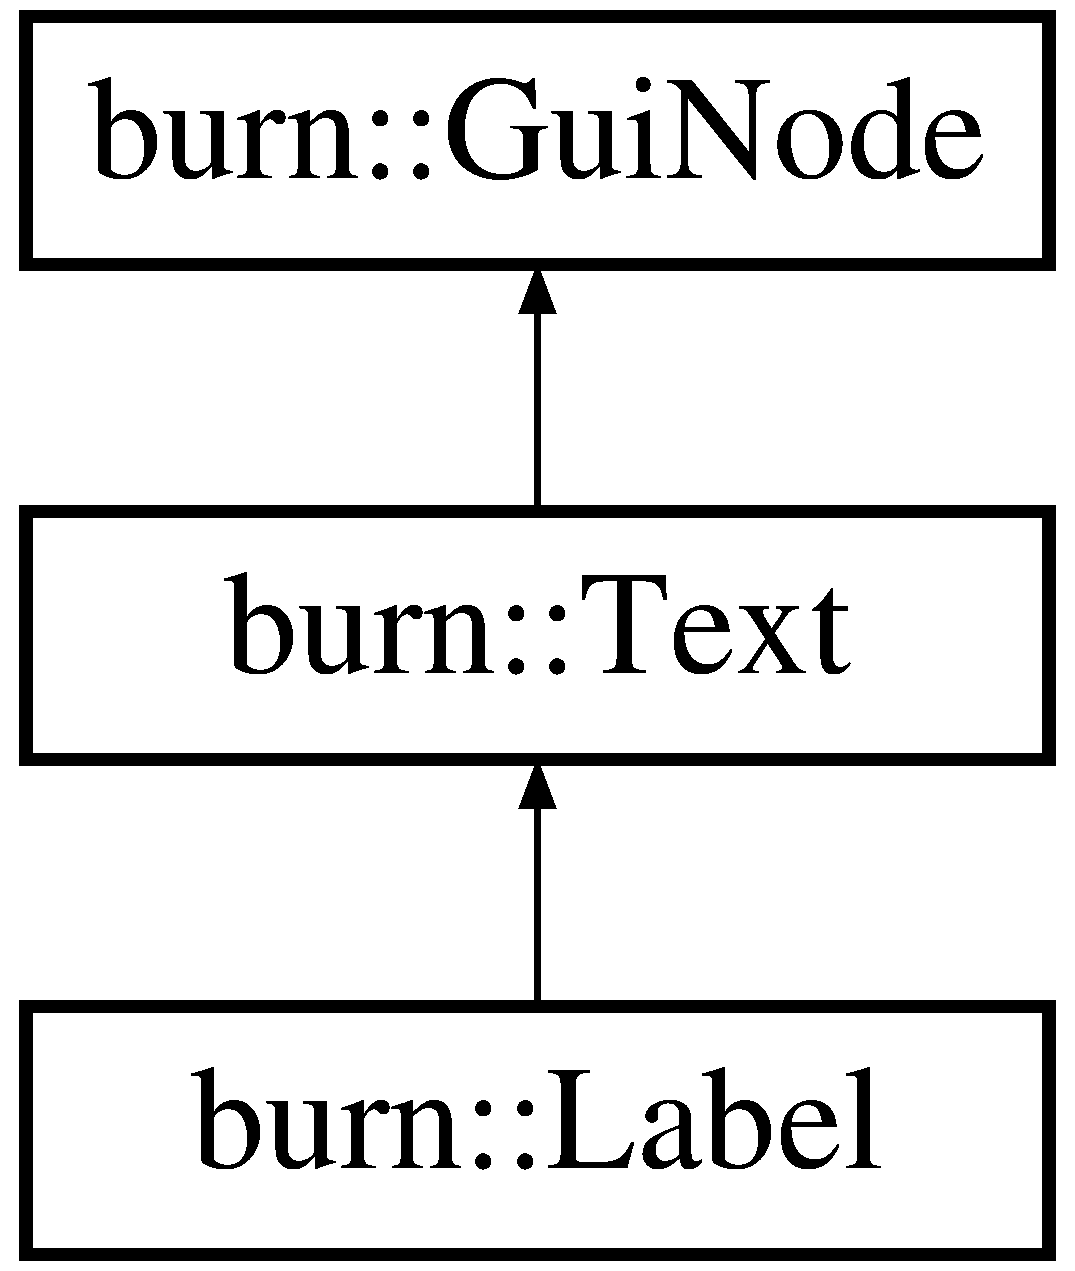
\includegraphics[height=3.000000cm]{classburn_1_1_label}
\end{center}
\end{figure}
\subsection*{Public Member Functions}
\begin{DoxyCompactItemize}
\item 
\hyperlink{classburn_1_1_label_a2fa54075b309e74c2bf0b8e1cf987404}{Label} ()
\item 
\hyperlink{classburn_1_1_label_a506c36c2a01f59620390597efb3014f8}{$\sim$\-Label} ()
\item 
virtual void \hyperlink{classburn_1_1_label_a23eaa7ccb0a68e6691a89133cb4254d5}{draw} ()
\item 
void \hyperlink{classburn_1_1_label_af0f6b8afde28a84cd81bc807c165b0ed}{set\-Background\-Color} (const \hyperlink{namespaceburn_a58a411b9d83c7970518a9250c1c78068}{Vector4f} \&color)
\item 
const \hyperlink{namespaceburn_a58a411b9d83c7970518a9250c1c78068}{Vector4f} \& \hyperlink{classburn_1_1_label_a0b89964384230c91c67a51f485ba39f7}{get\-Background\-Color} () const 
\item 
void \hyperlink{classburn_1_1_label_a13bbf6cc1170fd4ce2115a419ae937d7}{set\-Border} (const float \&border)
\item 
const float \& \hyperlink{classburn_1_1_label_a1c8c5359f4d4430f62fb19cb66b71829}{get\-Border} () const 
\end{DoxyCompactItemize}
\subsection*{Additional Inherited Members}


\subsection{Constructor \& Destructor Documentation}
\hypertarget{classburn_1_1_label_a2fa54075b309e74c2bf0b8e1cf987404}{\index{burn\-::\-Label@{burn\-::\-Label}!Label@{Label}}
\index{Label@{Label}!burn::Label@{burn\-::\-Label}}
\subsubsection[{Label}]{\setlength{\rightskip}{0pt plus 5cm}burn\-::\-Label\-::\-Label (
\begin{DoxyParamCaption}
{}
\end{DoxyParamCaption}
)}}\label{classburn_1_1_label_a2fa54075b309e74c2bf0b8e1cf987404}
\hypertarget{classburn_1_1_label_a506c36c2a01f59620390597efb3014f8}{\index{burn\-::\-Label@{burn\-::\-Label}!$\sim$\-Label@{$\sim$\-Label}}
\index{$\sim$\-Label@{$\sim$\-Label}!burn::Label@{burn\-::\-Label}}
\subsubsection[{$\sim$\-Label}]{\setlength{\rightskip}{0pt plus 5cm}burn\-::\-Label\-::$\sim$\-Label (
\begin{DoxyParamCaption}
{}
\end{DoxyParamCaption}
)}}\label{classburn_1_1_label_a506c36c2a01f59620390597efb3014f8}


\subsection{Member Function Documentation}
\hypertarget{classburn_1_1_label_a23eaa7ccb0a68e6691a89133cb4254d5}{\index{burn\-::\-Label@{burn\-::\-Label}!draw@{draw}}
\index{draw@{draw}!burn::Label@{burn\-::\-Label}}
\subsubsection[{draw}]{\setlength{\rightskip}{0pt plus 5cm}virtual void burn\-::\-Label\-::draw (
\begin{DoxyParamCaption}
{}
\end{DoxyParamCaption}
)\hspace{0.3cm}{\ttfamily [virtual]}}}\label{classburn_1_1_label_a23eaa7ccb0a68e6691a89133cb4254d5}


Reimplemented from \hyperlink{classburn_1_1_text_aa451ad17d21dc9c12cef712aa41914bf}{burn\-::\-Text}.

\hypertarget{classburn_1_1_label_a0b89964384230c91c67a51f485ba39f7}{\index{burn\-::\-Label@{burn\-::\-Label}!get\-Background\-Color@{get\-Background\-Color}}
\index{get\-Background\-Color@{get\-Background\-Color}!burn::Label@{burn\-::\-Label}}
\subsubsection[{get\-Background\-Color}]{\setlength{\rightskip}{0pt plus 5cm}const {\bf Vector4f}\& burn\-::\-Label\-::get\-Background\-Color (
\begin{DoxyParamCaption}
{}
\end{DoxyParamCaption}
) const}}\label{classburn_1_1_label_a0b89964384230c91c67a51f485ba39f7}
\hypertarget{classburn_1_1_label_a1c8c5359f4d4430f62fb19cb66b71829}{\index{burn\-::\-Label@{burn\-::\-Label}!get\-Border@{get\-Border}}
\index{get\-Border@{get\-Border}!burn::Label@{burn\-::\-Label}}
\subsubsection[{get\-Border}]{\setlength{\rightskip}{0pt plus 5cm}const float\& burn\-::\-Label\-::get\-Border (
\begin{DoxyParamCaption}
{}
\end{DoxyParamCaption}
) const}}\label{classburn_1_1_label_a1c8c5359f4d4430f62fb19cb66b71829}
\hypertarget{classburn_1_1_label_af0f6b8afde28a84cd81bc807c165b0ed}{\index{burn\-::\-Label@{burn\-::\-Label}!set\-Background\-Color@{set\-Background\-Color}}
\index{set\-Background\-Color@{set\-Background\-Color}!burn::Label@{burn\-::\-Label}}
\subsubsection[{set\-Background\-Color}]{\setlength{\rightskip}{0pt plus 5cm}void burn\-::\-Label\-::set\-Background\-Color (
\begin{DoxyParamCaption}
\item[{const {\bf Vector4f} \&}]{color}
\end{DoxyParamCaption}
)}}\label{classburn_1_1_label_af0f6b8afde28a84cd81bc807c165b0ed}
\hypertarget{classburn_1_1_label_a13bbf6cc1170fd4ce2115a419ae937d7}{\index{burn\-::\-Label@{burn\-::\-Label}!set\-Border@{set\-Border}}
\index{set\-Border@{set\-Border}!burn::Label@{burn\-::\-Label}}
\subsubsection[{set\-Border}]{\setlength{\rightskip}{0pt plus 5cm}void burn\-::\-Label\-::set\-Border (
\begin{DoxyParamCaption}
\item[{const float \&}]{border}
\end{DoxyParamCaption}
)}}\label{classburn_1_1_label_a13bbf6cc1170fd4ce2115a419ae937d7}


The documentation for this class was generated from the following file\-:\begin{DoxyCompactItemize}
\item 
include/\-Burngine/\-Graphics/\-Gui/\hyperlink{_label_8h}{Label.\-h}\end{DoxyCompactItemize}

\hypertarget{classburn_1_1_light}{\section{burn\-:\-:Light Class Reference}
\label{classburn_1_1_light}\index{burn\-::\-Light@{burn\-::\-Light}}
}


Inherits from \hyperlink{classburn_1_1_transformable}{Transformable}. Obviously the scale will have no effect.  




{\ttfamily \#include $<$Light.\-h$>$}

Inheritance diagram for burn\-:\-:Light\-:\begin{figure}[H]
\begin{center}
\leavevmode
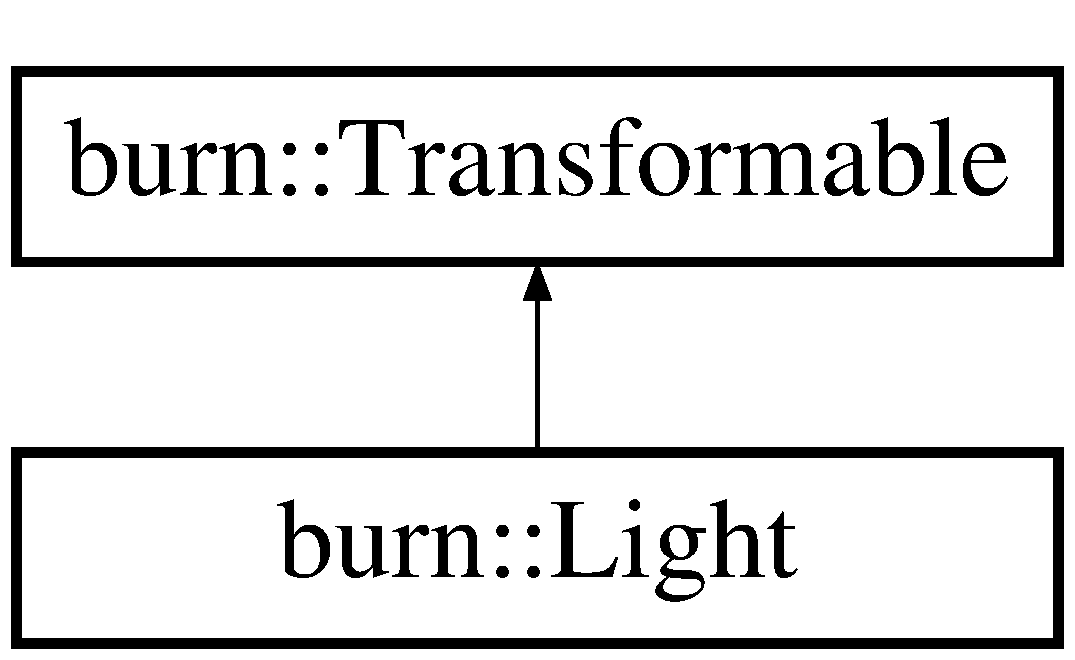
\includegraphics[height=2.000000cm]{classburn_1_1_light}
\end{center}
\end{figure}
\subsection*{Public Types}
\begin{DoxyCompactItemize}
\item 
enum \hyperlink{classburn_1_1_light_a8fa12cb3ae2a0eebbfbf5c59c2b4b599}{Type} \{ \hyperlink{classburn_1_1_light_a8fa12cb3ae2a0eebbfbf5c59c2b4b599a9e95c3ab6dc0c16260ba514a02151ce7}{P\-O\-I\-N\-T}, 
\hyperlink{classburn_1_1_light_a8fa12cb3ae2a0eebbfbf5c59c2b4b599a69cd23e3f1a59a02503370432fe42fd6}{S\-P\-O\-T}, 
\hyperlink{classburn_1_1_light_a8fa12cb3ae2a0eebbfbf5c59c2b4b599a25edb9fd19c152a1fbae29ec6a95b032}{D\-I\-R\-E\-C\-T\-I\-O\-N\-A\-L}
 \}
\end{DoxyCompactItemize}
\subsection*{Public Member Functions}
\begin{DoxyCompactItemize}
\item 
\hyperlink{classburn_1_1_light_a70a09e0609abe704f3e65d4790b6d6ce}{Light} (const \hyperlink{classburn_1_1_light_a8fa12cb3ae2a0eebbfbf5c59c2b4b599}{Type} \&type=\hyperlink{classburn_1_1_light_a8fa12cb3ae2a0eebbfbf5c59c2b4b599a9e95c3ab6dc0c16260ba514a02151ce7}{P\-O\-I\-N\-T}, const \hyperlink{namespaceburn_a9d6d349c94bc4dc9699427216128a0ef}{Vector3f} \&color=\hyperlink{namespaceburn_a9d6d349c94bc4dc9699427216128a0ef}{Vector3f}(1.\-0f, 1.\-0f, 1.\-0f), const float \&intensity=1.\-0f)
\item 
\hyperlink{classburn_1_1_light_af0fe1fa2f8f4527e80bd4ca80b2f6c4e}{$\sim$\-Light} ()
\item 
void \hyperlink{classburn_1_1_light_a6178f2826887a4aba596523b3e001604}{set\-Color} (const \hyperlink{namespaceburn_a9d6d349c94bc4dc9699427216128a0ef}{Vector3f} \&color)
\item 
const \hyperlink{namespaceburn_a9d6d349c94bc4dc9699427216128a0ef}{Vector3f} \& \hyperlink{classburn_1_1_light_a00de56025645f4c39d03b24e48f4eabf}{get\-Color} () const 
\item 
void \hyperlink{classburn_1_1_light_a798ae7d682b85dcede11a89047f19508}{set\-Intensity} (const float \&intensity)
\item 
const float \& \hyperlink{classburn_1_1_light_a0e826b840750ededc98e73f814c2de4a}{get\-Intensity} () const 
\item 
void \hyperlink{classburn_1_1_light_a1b0285cf5b58bc337a8d3ab9b4077554}{set\-Type} (const \hyperlink{classburn_1_1_light_a8fa12cb3ae2a0eebbfbf5c59c2b4b599}{Type} \&type)
\item 
const \hyperlink{classburn_1_1_light_a8fa12cb3ae2a0eebbfbf5c59c2b4b599}{Type} \& \hyperlink{classburn_1_1_light_aa96f8a2a736f033cd93f16467faad31b}{get\-Type} () const 
\end{DoxyCompactItemize}
\subsection*{Additional Inherited Members}


\subsection{Detailed Description}
Inherits from \hyperlink{classburn_1_1_transformable}{Transformable}. Obviously the scale will have no effect. 

\subsection{Member Enumeration Documentation}
\hypertarget{classburn_1_1_light_a8fa12cb3ae2a0eebbfbf5c59c2b4b599}{\index{burn\-::\-Light@{burn\-::\-Light}!Type@{Type}}
\index{Type@{Type}!burn::Light@{burn\-::\-Light}}
\subsubsection[{Type}]{\setlength{\rightskip}{0pt plus 5cm}enum {\bf burn\-::\-Light\-::\-Type}}}\label{classburn_1_1_light_a8fa12cb3ae2a0eebbfbf5c59c2b4b599}
\begin{Desc}
\item[Enumerator]\par
\begin{description}
\index{P\-O\-I\-N\-T@{P\-O\-I\-N\-T}!burn\-::\-Light@{burn\-::\-Light}}\index{burn\-::\-Light@{burn\-::\-Light}!P\-O\-I\-N\-T@{P\-O\-I\-N\-T}}\item[{\em 
\hypertarget{classburn_1_1_light_a8fa12cb3ae2a0eebbfbf5c59c2b4b599a9e95c3ab6dc0c16260ba514a02151ce7}{P\-O\-I\-N\-T}\label{classburn_1_1_light_a8fa12cb3ae2a0eebbfbf5c59c2b4b599a9e95c3ab6dc0c16260ba514a02151ce7}
}]\index{S\-P\-O\-T@{S\-P\-O\-T}!burn\-::\-Light@{burn\-::\-Light}}\index{burn\-::\-Light@{burn\-::\-Light}!S\-P\-O\-T@{S\-P\-O\-T}}\item[{\em 
\hypertarget{classburn_1_1_light_a8fa12cb3ae2a0eebbfbf5c59c2b4b599a69cd23e3f1a59a02503370432fe42fd6}{S\-P\-O\-T}\label{classburn_1_1_light_a8fa12cb3ae2a0eebbfbf5c59c2b4b599a69cd23e3f1a59a02503370432fe42fd6}
}]\index{D\-I\-R\-E\-C\-T\-I\-O\-N\-A\-L@{D\-I\-R\-E\-C\-T\-I\-O\-N\-A\-L}!burn\-::\-Light@{burn\-::\-Light}}\index{burn\-::\-Light@{burn\-::\-Light}!D\-I\-R\-E\-C\-T\-I\-O\-N\-A\-L@{D\-I\-R\-E\-C\-T\-I\-O\-N\-A\-L}}\item[{\em 
\hypertarget{classburn_1_1_light_a8fa12cb3ae2a0eebbfbf5c59c2b4b599a25edb9fd19c152a1fbae29ec6a95b032}{D\-I\-R\-E\-C\-T\-I\-O\-N\-A\-L}\label{classburn_1_1_light_a8fa12cb3ae2a0eebbfbf5c59c2b4b599a25edb9fd19c152a1fbae29ec6a95b032}
}]\end{description}
\end{Desc}


\subsection{Constructor \& Destructor Documentation}
\hypertarget{classburn_1_1_light_a70a09e0609abe704f3e65d4790b6d6ce}{\index{burn\-::\-Light@{burn\-::\-Light}!Light@{Light}}
\index{Light@{Light}!burn::Light@{burn\-::\-Light}}
\subsubsection[{Light}]{\setlength{\rightskip}{0pt plus 5cm}burn\-::\-Light\-::\-Light (
\begin{DoxyParamCaption}
\item[{const {\bf Type} \&}]{type = {\ttfamily {\bf P\-O\-I\-N\-T}}, }
\item[{const {\bf Vector3f} \&}]{color = {\ttfamily {\bf Vector3f}(1.0f,~1.0f,~1.0f)}, }
\item[{const float \&}]{intensity = {\ttfamily 1.0f}}
\end{DoxyParamCaption}
)}}\label{classburn_1_1_light_a70a09e0609abe704f3e65d4790b6d6ce}
\hypertarget{classburn_1_1_light_af0fe1fa2f8f4527e80bd4ca80b2f6c4e}{\index{burn\-::\-Light@{burn\-::\-Light}!$\sim$\-Light@{$\sim$\-Light}}
\index{$\sim$\-Light@{$\sim$\-Light}!burn::Light@{burn\-::\-Light}}
\subsubsection[{$\sim$\-Light}]{\setlength{\rightskip}{0pt plus 5cm}burn\-::\-Light\-::$\sim$\-Light (
\begin{DoxyParamCaption}
{}
\end{DoxyParamCaption}
)}}\label{classburn_1_1_light_af0fe1fa2f8f4527e80bd4ca80b2f6c4e}


\subsection{Member Function Documentation}
\hypertarget{classburn_1_1_light_a00de56025645f4c39d03b24e48f4eabf}{\index{burn\-::\-Light@{burn\-::\-Light}!get\-Color@{get\-Color}}
\index{get\-Color@{get\-Color}!burn::Light@{burn\-::\-Light}}
\subsubsection[{get\-Color}]{\setlength{\rightskip}{0pt plus 5cm}const {\bf Vector3f} \& burn\-::\-Light\-::get\-Color (
\begin{DoxyParamCaption}
{}
\end{DoxyParamCaption}
) const}}\label{classburn_1_1_light_a00de56025645f4c39d03b24e48f4eabf}
\hypertarget{classburn_1_1_light_a0e826b840750ededc98e73f814c2de4a}{\index{burn\-::\-Light@{burn\-::\-Light}!get\-Intensity@{get\-Intensity}}
\index{get\-Intensity@{get\-Intensity}!burn::Light@{burn\-::\-Light}}
\subsubsection[{get\-Intensity}]{\setlength{\rightskip}{0pt plus 5cm}const float \& burn\-::\-Light\-::get\-Intensity (
\begin{DoxyParamCaption}
{}
\end{DoxyParamCaption}
) const}}\label{classburn_1_1_light_a0e826b840750ededc98e73f814c2de4a}
\hypertarget{classburn_1_1_light_aa96f8a2a736f033cd93f16467faad31b}{\index{burn\-::\-Light@{burn\-::\-Light}!get\-Type@{get\-Type}}
\index{get\-Type@{get\-Type}!burn::Light@{burn\-::\-Light}}
\subsubsection[{get\-Type}]{\setlength{\rightskip}{0pt plus 5cm}const {\bf Light\-::\-Type} \& burn\-::\-Light\-::get\-Type (
\begin{DoxyParamCaption}
{}
\end{DoxyParamCaption}
) const}}\label{classburn_1_1_light_aa96f8a2a736f033cd93f16467faad31b}
\hypertarget{classburn_1_1_light_a6178f2826887a4aba596523b3e001604}{\index{burn\-::\-Light@{burn\-::\-Light}!set\-Color@{set\-Color}}
\index{set\-Color@{set\-Color}!burn::Light@{burn\-::\-Light}}
\subsubsection[{set\-Color}]{\setlength{\rightskip}{0pt plus 5cm}void burn\-::\-Light\-::set\-Color (
\begin{DoxyParamCaption}
\item[{const {\bf Vector3f} \&}]{color}
\end{DoxyParamCaption}
)}}\label{classburn_1_1_light_a6178f2826887a4aba596523b3e001604}
\hypertarget{classburn_1_1_light_a798ae7d682b85dcede11a89047f19508}{\index{burn\-::\-Light@{burn\-::\-Light}!set\-Intensity@{set\-Intensity}}
\index{set\-Intensity@{set\-Intensity}!burn::Light@{burn\-::\-Light}}
\subsubsection[{set\-Intensity}]{\setlength{\rightskip}{0pt plus 5cm}void burn\-::\-Light\-::set\-Intensity (
\begin{DoxyParamCaption}
\item[{const float \&}]{intensity}
\end{DoxyParamCaption}
)}}\label{classburn_1_1_light_a798ae7d682b85dcede11a89047f19508}
\hypertarget{classburn_1_1_light_a1b0285cf5b58bc337a8d3ab9b4077554}{\index{burn\-::\-Light@{burn\-::\-Light}!set\-Type@{set\-Type}}
\index{set\-Type@{set\-Type}!burn::Light@{burn\-::\-Light}}
\subsubsection[{set\-Type}]{\setlength{\rightskip}{0pt plus 5cm}void burn\-::\-Light\-::set\-Type (
\begin{DoxyParamCaption}
\item[{const {\bf Type} \&}]{type}
\end{DoxyParamCaption}
)}}\label{classburn_1_1_light_a1b0285cf5b58bc337a8d3ab9b4077554}


The documentation for this class was generated from the following files\-:\begin{DoxyCompactItemize}
\item 
include/\-Burngine/\-Graphics/\hyperlink{_light_8h}{Light.\-h}\item 
include/\-Burngine/\-Graphics/\hyperlink{_light_8cpp}{Light.\-cpp}\end{DoxyCompactItemize}

\hypertarget{classburn_1_1_material}{\section{burn\-:\-:Material Class Reference}
\label{classburn_1_1_material}\index{burn\-::\-Material@{burn\-::\-Material}}
}


{\ttfamily \#include $<$Material.\-h$>$}

\subsection*{Public Types}
\begin{DoxyCompactItemize}
\item 
enum \hyperlink{classburn_1_1_material_a704108f8bb133e1911495b84bd0826b8}{Flag} \{ \hyperlink{classburn_1_1_material_a704108f8bb133e1911495b84bd0826b8a20ce785514749ab3909bc895127e2823}{L\-I\-G\-H\-T\-I\-N\-G} = 0, 
\hyperlink{classburn_1_1_material_a704108f8bb133e1911495b84bd0826b8a76028dd1ab583178b4e69a0894260c78}{C\-O\-U\-N\-T}
 \}
\item 
enum \hyperlink{classburn_1_1_material_a2d219315cf05e59bbffe8e3831cc6c43}{Type} \{ \hyperlink{classburn_1_1_material_a2d219315cf05e59bbffe8e3831cc6c43ae346efa71a38eb8fcbcba453a89c6aa4}{S\-O\-L\-I\-D\-\_\-\-C\-O\-L\-O\-R} = 0, 
\hyperlink{classburn_1_1_material_a2d219315cf05e59bbffe8e3831cc6c43a56549fc4dfe95a8e1fbb6bb48560f084}{T\-E\-X\-T\-U\-R\-E\-D}
 \}
\end{DoxyCompactItemize}
\subsection*{Public Member Functions}
\begin{DoxyCompactItemize}
\item 
\hyperlink{classburn_1_1_material_a790cff05e96bd7956582777754a56a34}{Material} ()
\begin{DoxyCompactList}\small\item\em The default constructor Default values\-: \end{DoxyCompactList}\item 
\hyperlink{classburn_1_1_material_a449723d0d12182275e5d0d8a6a01f41d}{$\sim$\-Material} ()
\begin{DoxyCompactList}\small\item\em The default destructor. \end{DoxyCompactList}\item 
void \hyperlink{classburn_1_1_material_a833037afe81bc0aa52ceb4581b66087f}{set\-Flag} (\hyperlink{classburn_1_1_material_a704108f8bb133e1911495b84bd0826b8}{Flag} flag, bool enabled=true)
\begin{DoxyCompactList}\small\item\em Sets the specified flag on true or false. \end{DoxyCompactList}\item 
void \hyperlink{classburn_1_1_material_a287ad604c643dc76fc07d27b45ceecd2}{set\-Type} (\hyperlink{classburn_1_1_material_a2d219315cf05e59bbffe8e3831cc6c43}{Type} type)
\begin{DoxyCompactList}\small\item\em Sets the type of the material. The \hyperlink{classburn_1_1_scene_node}{Scene\-Node} will choose the right \hyperlink{classburn_1_1_shader}{Shader}. \end{DoxyCompactList}\item 
const \hyperlink{classburn_1_1_material_a2d219315cf05e59bbffe8e3831cc6c43}{Type} \& \hyperlink{classburn_1_1_material_afce65f6bded42bd03552741fe70649d8}{get\-Type} () const 
\begin{DoxyCompactList}\small\item\em Returns the current type. \end{DoxyCompactList}\item 
bool \hyperlink{classburn_1_1_material_afa32027c9de752c96b74e08b3f1e42af}{is\-Flag\-Set} (\hyperlink{classburn_1_1_material_a704108f8bb133e1911495b84bd0826b8}{Flag} flag) const 
\begin{DoxyCompactList}\small\item\em Returns the current status of a flag. \end{DoxyCompactList}\item 
void \hyperlink{classburn_1_1_material_ae50bc615e9bb17bc9eb232345fb1e776}{set\-Specular\-Color} (const \hyperlink{namespaceburn_afdd7cfb352b9612432faf6947b6fff74}{Vector3f} \&color)
\item 
const \hyperlink{namespaceburn_afdd7cfb352b9612432faf6947b6fff74}{Vector3f} \& \hyperlink{classburn_1_1_material_ab7d639a776c308b57eb0b3210b27449e}{get\-Specular\-Color} () const 
\item 
void \hyperlink{classburn_1_1_material_a0b50c4daafb286d54d5159bc93fc695c}{set\-Diffuse\-Color} (const \hyperlink{namespaceburn_afdd7cfb352b9612432faf6947b6fff74}{Vector3f} \&color)
\item 
const \hyperlink{namespaceburn_afdd7cfb352b9612432faf6947b6fff74}{Vector3f} \& \hyperlink{classburn_1_1_material_acc1501d3c24c0bf6c2f120d1e1a67c0f}{get\-Diffuse\-Color} () const 
\item 
void \hyperlink{classburn_1_1_material_a730e2d8f5d444f6ce45e1f25a4f424d6}{set\-Index} (const unsigned int \&index)
\item 
const unsigned int \& \hyperlink{classburn_1_1_material_a7e30e5e26a8a9648910ef17901452d20}{get\-Index} () const 
\item 
void \hyperlink{classburn_1_1_material_a016895c77f4fd7393ab263ac7455e5a2}{use\-Diffuse\-Color} (bool should\-Use\-Diffuse=true)
\item 
bool \hyperlink{classburn_1_1_material_a4f2d46a41409a068985c7377eeb1f3c4}{is\-Using\-Diffuse\-Color} () const 
\end{DoxyCompactItemize}


\subsection{Member Enumeration Documentation}
\hypertarget{classburn_1_1_material_a704108f8bb133e1911495b84bd0826b8}{\index{burn\-::\-Material@{burn\-::\-Material}!Flag@{Flag}}
\index{Flag@{Flag}!burn::Material@{burn\-::\-Material}}
\subsubsection[{Flag}]{\setlength{\rightskip}{0pt plus 5cm}enum {\bf burn\-::\-Material\-::\-Flag}}}\label{classburn_1_1_material_a704108f8bb133e1911495b84bd0826b8}
\begin{Desc}
\item[Enumerator]\par
\begin{description}
\index{L\-I\-G\-H\-T\-I\-N\-G@{L\-I\-G\-H\-T\-I\-N\-G}!burn\-::\-Material@{burn\-::\-Material}}\index{burn\-::\-Material@{burn\-::\-Material}!L\-I\-G\-H\-T\-I\-N\-G@{L\-I\-G\-H\-T\-I\-N\-G}}\item[{\em 
\hypertarget{classburn_1_1_material_a704108f8bb133e1911495b84bd0826b8a20ce785514749ab3909bc895127e2823}{L\-I\-G\-H\-T\-I\-N\-G}\label{classburn_1_1_material_a704108f8bb133e1911495b84bd0826b8a20ce785514749ab3909bc895127e2823}
}]\index{C\-O\-U\-N\-T@{C\-O\-U\-N\-T}!burn\-::\-Material@{burn\-::\-Material}}\index{burn\-::\-Material@{burn\-::\-Material}!C\-O\-U\-N\-T@{C\-O\-U\-N\-T}}\item[{\em 
\hypertarget{classburn_1_1_material_a704108f8bb133e1911495b84bd0826b8a76028dd1ab583178b4e69a0894260c78}{C\-O\-U\-N\-T}\label{classburn_1_1_material_a704108f8bb133e1911495b84bd0826b8a76028dd1ab583178b4e69a0894260c78}
}]\end{description}
\end{Desc}
\hypertarget{classburn_1_1_material_a2d219315cf05e59bbffe8e3831cc6c43}{\index{burn\-::\-Material@{burn\-::\-Material}!Type@{Type}}
\index{Type@{Type}!burn::Material@{burn\-::\-Material}}
\subsubsection[{Type}]{\setlength{\rightskip}{0pt plus 5cm}enum {\bf burn\-::\-Material\-::\-Type}}}\label{classburn_1_1_material_a2d219315cf05e59bbffe8e3831cc6c43}
\begin{Desc}
\item[Enumerator]\par
\begin{description}
\index{S\-O\-L\-I\-D\-\_\-\-C\-O\-L\-O\-R@{S\-O\-L\-I\-D\-\_\-\-C\-O\-L\-O\-R}!burn\-::\-Material@{burn\-::\-Material}}\index{burn\-::\-Material@{burn\-::\-Material}!S\-O\-L\-I\-D\-\_\-\-C\-O\-L\-O\-R@{S\-O\-L\-I\-D\-\_\-\-C\-O\-L\-O\-R}}\item[{\em 
\hypertarget{classburn_1_1_material_a2d219315cf05e59bbffe8e3831cc6c43ae346efa71a38eb8fcbcba453a89c6aa4}{S\-O\-L\-I\-D\-\_\-\-C\-O\-L\-O\-R}\label{classburn_1_1_material_a2d219315cf05e59bbffe8e3831cc6c43ae346efa71a38eb8fcbcba453a89c6aa4}
}]\index{T\-E\-X\-T\-U\-R\-E\-D@{T\-E\-X\-T\-U\-R\-E\-D}!burn\-::\-Material@{burn\-::\-Material}}\index{burn\-::\-Material@{burn\-::\-Material}!T\-E\-X\-T\-U\-R\-E\-D@{T\-E\-X\-T\-U\-R\-E\-D}}\item[{\em 
\hypertarget{classburn_1_1_material_a2d219315cf05e59bbffe8e3831cc6c43a56549fc4dfe95a8e1fbb6bb48560f084}{T\-E\-X\-T\-U\-R\-E\-D}\label{classburn_1_1_material_a2d219315cf05e59bbffe8e3831cc6c43a56549fc4dfe95a8e1fbb6bb48560f084}
}]\end{description}
\end{Desc}


\subsection{Constructor \& Destructor Documentation}
\hypertarget{classburn_1_1_material_a790cff05e96bd7956582777754a56a34}{\index{burn\-::\-Material@{burn\-::\-Material}!Material@{Material}}
\index{Material@{Material}!burn::Material@{burn\-::\-Material}}
\subsubsection[{Material}]{\setlength{\rightskip}{0pt plus 5cm}burn\-::\-Material\-::\-Material (
\begin{DoxyParamCaption}
{}
\end{DoxyParamCaption}
)}}\label{classburn_1_1_material_a790cff05e96bd7956582777754a56a34}


The default constructor Default values\-: 


\begin{DoxyItemize}
\item Type\-: S\-O\-L\-I\-D\-\_\-\-C\-O\-L\-O\-R
\item Flag\mbox{[}L\-I\-G\-H\-T\-I\-N\-G\mbox{]}\-: false 
\end{DoxyItemize}\hypertarget{classburn_1_1_material_a449723d0d12182275e5d0d8a6a01f41d}{\index{burn\-::\-Material@{burn\-::\-Material}!$\sim$\-Material@{$\sim$\-Material}}
\index{$\sim$\-Material@{$\sim$\-Material}!burn::Material@{burn\-::\-Material}}
\subsubsection[{$\sim$\-Material}]{\setlength{\rightskip}{0pt plus 5cm}burn\-::\-Material\-::$\sim$\-Material (
\begin{DoxyParamCaption}
{}
\end{DoxyParamCaption}
)}}\label{classburn_1_1_material_a449723d0d12182275e5d0d8a6a01f41d}


The default destructor. 



\subsection{Member Function Documentation}
\hypertarget{classburn_1_1_material_acc1501d3c24c0bf6c2f120d1e1a67c0f}{\index{burn\-::\-Material@{burn\-::\-Material}!get\-Diffuse\-Color@{get\-Diffuse\-Color}}
\index{get\-Diffuse\-Color@{get\-Diffuse\-Color}!burn::Material@{burn\-::\-Material}}
\subsubsection[{get\-Diffuse\-Color}]{\setlength{\rightskip}{0pt plus 5cm}const {\bf Vector3f}\& burn\-::\-Material\-::get\-Diffuse\-Color (
\begin{DoxyParamCaption}
{}
\end{DoxyParamCaption}
) const}}\label{classburn_1_1_material_acc1501d3c24c0bf6c2f120d1e1a67c0f}
\hypertarget{classburn_1_1_material_a7e30e5e26a8a9648910ef17901452d20}{\index{burn\-::\-Material@{burn\-::\-Material}!get\-Index@{get\-Index}}
\index{get\-Index@{get\-Index}!burn::Material@{burn\-::\-Material}}
\subsubsection[{get\-Index}]{\setlength{\rightskip}{0pt plus 5cm}const unsigned int\& burn\-::\-Material\-::get\-Index (
\begin{DoxyParamCaption}
{}
\end{DoxyParamCaption}
) const}}\label{classburn_1_1_material_a7e30e5e26a8a9648910ef17901452d20}
\hypertarget{classburn_1_1_material_ab7d639a776c308b57eb0b3210b27449e}{\index{burn\-::\-Material@{burn\-::\-Material}!get\-Specular\-Color@{get\-Specular\-Color}}
\index{get\-Specular\-Color@{get\-Specular\-Color}!burn::Material@{burn\-::\-Material}}
\subsubsection[{get\-Specular\-Color}]{\setlength{\rightskip}{0pt plus 5cm}const {\bf Vector3f}\& burn\-::\-Material\-::get\-Specular\-Color (
\begin{DoxyParamCaption}
{}
\end{DoxyParamCaption}
) const}}\label{classburn_1_1_material_ab7d639a776c308b57eb0b3210b27449e}
\hypertarget{classburn_1_1_material_afce65f6bded42bd03552741fe70649d8}{\index{burn\-::\-Material@{burn\-::\-Material}!get\-Type@{get\-Type}}
\index{get\-Type@{get\-Type}!burn::Material@{burn\-::\-Material}}
\subsubsection[{get\-Type}]{\setlength{\rightskip}{0pt plus 5cm}const {\bf Type}\& burn\-::\-Material\-::get\-Type (
\begin{DoxyParamCaption}
{}
\end{DoxyParamCaption}
) const}}\label{classburn_1_1_material_afce65f6bded42bd03552741fe70649d8}


Returns the current type. 

\begin{DoxyReturn}{Returns}
The current materialtype
\end{DoxyReturn}
\begin{DoxySeeAlso}{See Also}
\hyperlink{classburn_1_1_material_a287ad604c643dc76fc07d27b45ceecd2}{set\-Type()} 
\end{DoxySeeAlso}
\hypertarget{classburn_1_1_material_afa32027c9de752c96b74e08b3f1e42af}{\index{burn\-::\-Material@{burn\-::\-Material}!is\-Flag\-Set@{is\-Flag\-Set}}
\index{is\-Flag\-Set@{is\-Flag\-Set}!burn::Material@{burn\-::\-Material}}
\subsubsection[{is\-Flag\-Set}]{\setlength{\rightskip}{0pt plus 5cm}bool burn\-::\-Material\-::is\-Flag\-Set (
\begin{DoxyParamCaption}
\item[{{\bf Flag}}]{flag}
\end{DoxyParamCaption}
) const}}\label{classburn_1_1_material_afa32027c9de752c96b74e08b3f1e42af}


Returns the current status of a flag. 


\begin{DoxyParams}{Parameters}
{\em flag} & The flag to check\\
\hline
\end{DoxyParams}
\begin{DoxyReturn}{Returns}
Status of a flag.
\end{DoxyReturn}
\begin{DoxySeeAlso}{See Also}
\hyperlink{classburn_1_1_material_a833037afe81bc0aa52ceb4581b66087f}{set\-Flag()} 
\end{DoxySeeAlso}
\hypertarget{classburn_1_1_material_a4f2d46a41409a068985c7377eeb1f3c4}{\index{burn\-::\-Material@{burn\-::\-Material}!is\-Using\-Diffuse\-Color@{is\-Using\-Diffuse\-Color}}
\index{is\-Using\-Diffuse\-Color@{is\-Using\-Diffuse\-Color}!burn::Material@{burn\-::\-Material}}
\subsubsection[{is\-Using\-Diffuse\-Color}]{\setlength{\rightskip}{0pt plus 5cm}bool burn\-::\-Material\-::is\-Using\-Diffuse\-Color (
\begin{DoxyParamCaption}
{}
\end{DoxyParamCaption}
) const}}\label{classburn_1_1_material_a4f2d46a41409a068985c7377eeb1f3c4}
\hypertarget{classburn_1_1_material_a0b50c4daafb286d54d5159bc93fc695c}{\index{burn\-::\-Material@{burn\-::\-Material}!set\-Diffuse\-Color@{set\-Diffuse\-Color}}
\index{set\-Diffuse\-Color@{set\-Diffuse\-Color}!burn::Material@{burn\-::\-Material}}
\subsubsection[{set\-Diffuse\-Color}]{\setlength{\rightskip}{0pt plus 5cm}void burn\-::\-Material\-::set\-Diffuse\-Color (
\begin{DoxyParamCaption}
\item[{const {\bf Vector3f} \&}]{color}
\end{DoxyParamCaption}
)}}\label{classburn_1_1_material_a0b50c4daafb286d54d5159bc93fc695c}
\hypertarget{classburn_1_1_material_a833037afe81bc0aa52ceb4581b66087f}{\index{burn\-::\-Material@{burn\-::\-Material}!set\-Flag@{set\-Flag}}
\index{set\-Flag@{set\-Flag}!burn::Material@{burn\-::\-Material}}
\subsubsection[{set\-Flag}]{\setlength{\rightskip}{0pt plus 5cm}void burn\-::\-Material\-::set\-Flag (
\begin{DoxyParamCaption}
\item[{{\bf Flag}}]{flag, }
\item[{bool}]{enabled = {\ttfamily true}}
\end{DoxyParamCaption}
)}}\label{classburn_1_1_material_a833037afe81bc0aa52ceb4581b66087f}


Sets the specified flag on true or false. 


\begin{DoxyParams}{Parameters}
{\em flag} & The flag to set \\
\hline
{\em enabled} & Sets the specified flag on true or false\\
\hline
\end{DoxyParams}
\begin{DoxySeeAlso}{See Also}
\hyperlink{classburn_1_1_material_afa32027c9de752c96b74e08b3f1e42af}{is\-Flag\-Set()} 
\end{DoxySeeAlso}
\hypertarget{classburn_1_1_material_a730e2d8f5d444f6ce45e1f25a4f424d6}{\index{burn\-::\-Material@{burn\-::\-Material}!set\-Index@{set\-Index}}
\index{set\-Index@{set\-Index}!burn::Material@{burn\-::\-Material}}
\subsubsection[{set\-Index}]{\setlength{\rightskip}{0pt plus 5cm}void burn\-::\-Material\-::set\-Index (
\begin{DoxyParamCaption}
\item[{const unsigned int \&}]{index}
\end{DoxyParamCaption}
)}}\label{classburn_1_1_material_a730e2d8f5d444f6ce45e1f25a4f424d6}
\hypertarget{classburn_1_1_material_ae50bc615e9bb17bc9eb232345fb1e776}{\index{burn\-::\-Material@{burn\-::\-Material}!set\-Specular\-Color@{set\-Specular\-Color}}
\index{set\-Specular\-Color@{set\-Specular\-Color}!burn::Material@{burn\-::\-Material}}
\subsubsection[{set\-Specular\-Color}]{\setlength{\rightskip}{0pt plus 5cm}void burn\-::\-Material\-::set\-Specular\-Color (
\begin{DoxyParamCaption}
\item[{const {\bf Vector3f} \&}]{color}
\end{DoxyParamCaption}
)}}\label{classburn_1_1_material_ae50bc615e9bb17bc9eb232345fb1e776}
\hypertarget{classburn_1_1_material_a287ad604c643dc76fc07d27b45ceecd2}{\index{burn\-::\-Material@{burn\-::\-Material}!set\-Type@{set\-Type}}
\index{set\-Type@{set\-Type}!burn::Material@{burn\-::\-Material}}
\subsubsection[{set\-Type}]{\setlength{\rightskip}{0pt plus 5cm}void burn\-::\-Material\-::set\-Type (
\begin{DoxyParamCaption}
\item[{{\bf Type}}]{type}
\end{DoxyParamCaption}
)}}\label{classburn_1_1_material_a287ad604c643dc76fc07d27b45ceecd2}


Sets the type of the material. The \hyperlink{classburn_1_1_scene_node}{Scene\-Node} will choose the right \hyperlink{classburn_1_1_shader}{Shader}. 


\begin{DoxyParams}{Parameters}
{\em type} & The materialtype.\\
\hline
\end{DoxyParams}
\begin{DoxySeeAlso}{See Also}
\hyperlink{classburn_1_1_material_afce65f6bded42bd03552741fe70649d8}{get\-Type()}
\end{DoxySeeAlso}
\begin{DoxyNote}{Note}
Ensure that you have loaded the \hyperlink{structburn_1_1_burngine_shaders}{Burngine\-Shaders} before renering. E.\-g. by calling Burngine\-Shaders\-::load\-All\-Shaders() 
\end{DoxyNote}
\hypertarget{classburn_1_1_material_a016895c77f4fd7393ab263ac7455e5a2}{\index{burn\-::\-Material@{burn\-::\-Material}!use\-Diffuse\-Color@{use\-Diffuse\-Color}}
\index{use\-Diffuse\-Color@{use\-Diffuse\-Color}!burn::Material@{burn\-::\-Material}}
\subsubsection[{use\-Diffuse\-Color}]{\setlength{\rightskip}{0pt plus 5cm}void burn\-::\-Material\-::use\-Diffuse\-Color (
\begin{DoxyParamCaption}
\item[{bool}]{should\-Use\-Diffuse = {\ttfamily true}}
\end{DoxyParamCaption}
)}}\label{classburn_1_1_material_a016895c77f4fd7393ab263ac7455e5a2}


The documentation for this class was generated from the following file\-:\begin{DoxyCompactItemize}
\item 
include/\-Burngine/\-Graphics/\-Scene/\hyperlink{_material_8h}{Material.\-h}\end{DoxyCompactItemize}

\hypertarget{classburn_1_1_mesh}{\section{burn\-:\-:Mesh Class Reference}
\label{classburn_1_1_mesh}\index{burn\-::\-Mesh@{burn\-::\-Mesh}}
}


{\ttfamily \#include $<$Mesh.\-h$>$}

\subsection*{Public Member Functions}
\begin{DoxyCompactItemize}
\item 
\hyperlink{classburn_1_1_mesh_a35d4706a490d0f2bb190b6b785621e07}{Mesh} ()
\begin{DoxyCompactList}\small\item\em The default constructor. \end{DoxyCompactList}\item 
\hyperlink{classburn_1_1_mesh_ad8b2e6283ea14b3943a8945ab7f2d27d}{$\sim$\-Mesh} ()
\begin{DoxyCompactList}\small\item\em The default destructor. \end{DoxyCompactList}\item 
bool \hyperlink{classburn_1_1_mesh_a3179d5730bfcf0e781b1c0daebfc7439}{load\-From\-File} (const std\-::string \&file)
\begin{DoxyCompactList}\small\item\em Loads a 3\-D-\/model into the \hyperlink{classburn_1_1_mesh}{Mesh} object. It uses the assimp importer, so it supports the files that assimp does. \end{DoxyCompactList}\item 
void \hyperlink{classburn_1_1_mesh_ae0996bd5d561cdf7b26e27c713facea7}{set\-Vertices} (const std\-::vector$<$ \hyperlink{classburn_1_1_vertex}{Vertex} $>$ \&vertices)
\begin{DoxyCompactList}\small\item\em Sets the vertices of the mesh, so that they can be used for rendering later on. \end{DoxyCompactList}\item 
size\-\_\-t \hyperlink{classburn_1_1_mesh_a076016c8452ff794880480626394e44c}{get\-Vertex\-Count} () const 
\begin{DoxyCompactList}\small\item\em Returns the count of the vertices which the mesh is holding. \end{DoxyCompactList}\item 
const G\-Luint \& \hyperlink{classburn_1_1_mesh_a617b88d25c58c342f02751d67cb5e29b}{get\-Position\-Buffer} () const 
\begin{DoxyCompactList}\small\item\em Returns the id of the position-\/buffer. This is used mostly internally. But you can check the buffer by comparing the returned value with 0. \end{DoxyCompactList}\item 
const G\-Luint \& \hyperlink{classburn_1_1_mesh_ad571f57e9a162b86585c0b3f288bbfc6}{get\-Normal\-Buffer} () const 
\begin{DoxyCompactList}\small\item\em Returns the id of the normal-\/buffer. This is used mostly internally. But you can check the buffer by comparing the returned value with 0. \end{DoxyCompactList}\item 
const G\-Luint \& \hyperlink{classburn_1_1_mesh_ae8757bde80c135f9d8e8e0291e00ffe5}{get\-Color\-Buffer} () const 
\begin{DoxyCompactList}\small\item\em Returns the id of the color-\/buffer. This is used mostly internally. But you can check the buffer by comparing the returned value with 0. \end{DoxyCompactList}\item 
const G\-Luint \& \hyperlink{classburn_1_1_mesh_a5bcc126c9f06b9f04549b02328f2fc72}{get\-Uv\-Buffer} () const 
\begin{DoxyCompactList}\small\item\em Returns the id of the U\-V-\/buffer. This is used mostly internally. But you can check the buffer by comparing the returned value with 0. \end{DoxyCompactList}\item 
void \hyperlink{classburn_1_1_mesh_a2457c00cd236e5933e725bb1d55db0d9}{set\-Texture} (const \hyperlink{classburn_1_1_texture}{Texture} \&texture)
\begin{DoxyCompactList}\small\item\em Sets the \hyperlink{classburn_1_1_texture}{Texture} of the mesh. \end{DoxyCompactList}\item 
const \hyperlink{classburn_1_1_texture}{Texture} \& \hyperlink{classburn_1_1_mesh_acbea44f2a2683c44728bb17e4691d406}{get\-Texture} () const 
\begin{DoxyCompactList}\small\item\em Returns the current \hyperlink{classburn_1_1_texture}{Texture} of the mesh. \end{DoxyCompactList}\item 
\hyperlink{classburn_1_1_material}{Material} \& \hyperlink{classburn_1_1_mesh_a7e3f6168e3bb37e5c30323c5e19b85cc}{get\-Material} ()
\begin{DoxyCompactList}\small\item\em Returns the material that the node is using. \end{DoxyCompactList}\item 
void \hyperlink{classburn_1_1_mesh_a2ff24f1eb82cb417062e8d1ec179d8bd}{set\-Material} (\hyperlink{classburn_1_1_material}{Material} \&material)
\begin{DoxyCompactList}\small\item\em Sets the material of the node. Influences the rendering behaviour. \end{DoxyCompactList}\item 
void \hyperlink{classburn_1_1_mesh_a4880e1e9d0580cd08064290fe4c3d3a0}{update} ()
\item 
void \hyperlink{classburn_1_1_mesh_ad9d9b1c1d6a9486e65e384f28aa009d5}{force\-Update} ()
\end{DoxyCompactItemize}


\subsection{Constructor \& Destructor Documentation}
\hypertarget{classburn_1_1_mesh_a35d4706a490d0f2bb190b6b785621e07}{\index{burn\-::\-Mesh@{burn\-::\-Mesh}!Mesh@{Mesh}}
\index{Mesh@{Mesh}!burn::Mesh@{burn\-::\-Mesh}}
\subsubsection[{Mesh}]{\setlength{\rightskip}{0pt plus 5cm}burn\-::\-Mesh\-::\-Mesh (
\begin{DoxyParamCaption}
{}
\end{DoxyParamCaption}
)}}\label{classburn_1_1_mesh_a35d4706a490d0f2bb190b6b785621e07}


The default constructor. 

\hypertarget{classburn_1_1_mesh_ad8b2e6283ea14b3943a8945ab7f2d27d}{\index{burn\-::\-Mesh@{burn\-::\-Mesh}!$\sim$\-Mesh@{$\sim$\-Mesh}}
\index{$\sim$\-Mesh@{$\sim$\-Mesh}!burn::Mesh@{burn\-::\-Mesh}}
\subsubsection[{$\sim$\-Mesh}]{\setlength{\rightskip}{0pt plus 5cm}burn\-::\-Mesh\-::$\sim$\-Mesh (
\begin{DoxyParamCaption}
{}
\end{DoxyParamCaption}
)}}\label{classburn_1_1_mesh_ad8b2e6283ea14b3943a8945ab7f2d27d}


The default destructor. 



\subsection{Member Function Documentation}
\hypertarget{classburn_1_1_mesh_ad9d9b1c1d6a9486e65e384f28aa009d5}{\index{burn\-::\-Mesh@{burn\-::\-Mesh}!force\-Update@{force\-Update}}
\index{force\-Update@{force\-Update}!burn::Mesh@{burn\-::\-Mesh}}
\subsubsection[{force\-Update}]{\setlength{\rightskip}{0pt plus 5cm}void burn\-::\-Mesh\-::force\-Update (
\begin{DoxyParamCaption}
{}
\end{DoxyParamCaption}
)}}\label{classburn_1_1_mesh_ad9d9b1c1d6a9486e65e384f28aa009d5}
\hypertarget{classburn_1_1_mesh_ae8757bde80c135f9d8e8e0291e00ffe5}{\index{burn\-::\-Mesh@{burn\-::\-Mesh}!get\-Color\-Buffer@{get\-Color\-Buffer}}
\index{get\-Color\-Buffer@{get\-Color\-Buffer}!burn::Mesh@{burn\-::\-Mesh}}
\subsubsection[{get\-Color\-Buffer}]{\setlength{\rightskip}{0pt plus 5cm}const G\-Luint \& burn\-::\-Mesh\-::get\-Color\-Buffer (
\begin{DoxyParamCaption}
{}
\end{DoxyParamCaption}
) const}}\label{classburn_1_1_mesh_ae8757bde80c135f9d8e8e0291e00ffe5}


Returns the id of the color-\/buffer. This is used mostly internally. But you can check the buffer by comparing the returned value with 0. 

\begin{DoxyReturn}{Returns}
Returns the id of the color-\/buffer or 0 if no color-\/buffer exists 
\end{DoxyReturn}
\hypertarget{classburn_1_1_mesh_a7e3f6168e3bb37e5c30323c5e19b85cc}{\index{burn\-::\-Mesh@{burn\-::\-Mesh}!get\-Material@{get\-Material}}
\index{get\-Material@{get\-Material}!burn::Mesh@{burn\-::\-Mesh}}
\subsubsection[{get\-Material}]{\setlength{\rightskip}{0pt plus 5cm}{\bf Material} \& burn\-::\-Mesh\-::get\-Material (
\begin{DoxyParamCaption}
{}
\end{DoxyParamCaption}
)}}\label{classburn_1_1_mesh_a7e3f6168e3bb37e5c30323c5e19b85cc}


Returns the material that the node is using. 

\begin{DoxyReturn}{Returns}
The \hyperlink{classburn_1_1_material}{Material} of the node.
\end{DoxyReturn}
\begin{DoxySeeAlso}{See Also}
\hyperlink{classburn_1_1_mesh_a2ff24f1eb82cb417062e8d1ec179d8bd}{set\-Material()} 
\end{DoxySeeAlso}
\hypertarget{classburn_1_1_mesh_ad571f57e9a162b86585c0b3f288bbfc6}{\index{burn\-::\-Mesh@{burn\-::\-Mesh}!get\-Normal\-Buffer@{get\-Normal\-Buffer}}
\index{get\-Normal\-Buffer@{get\-Normal\-Buffer}!burn::Mesh@{burn\-::\-Mesh}}
\subsubsection[{get\-Normal\-Buffer}]{\setlength{\rightskip}{0pt plus 5cm}const G\-Luint \& burn\-::\-Mesh\-::get\-Normal\-Buffer (
\begin{DoxyParamCaption}
{}
\end{DoxyParamCaption}
) const}}\label{classburn_1_1_mesh_ad571f57e9a162b86585c0b3f288bbfc6}


Returns the id of the normal-\/buffer. This is used mostly internally. But you can check the buffer by comparing the returned value with 0. 

\begin{DoxyReturn}{Returns}
Returns the id of the normal-\/buffer or 0 if no normal-\/buffer exists 
\end{DoxyReturn}
\hypertarget{classburn_1_1_mesh_a617b88d25c58c342f02751d67cb5e29b}{\index{burn\-::\-Mesh@{burn\-::\-Mesh}!get\-Position\-Buffer@{get\-Position\-Buffer}}
\index{get\-Position\-Buffer@{get\-Position\-Buffer}!burn::Mesh@{burn\-::\-Mesh}}
\subsubsection[{get\-Position\-Buffer}]{\setlength{\rightskip}{0pt plus 5cm}const G\-Luint \& burn\-::\-Mesh\-::get\-Position\-Buffer (
\begin{DoxyParamCaption}
{}
\end{DoxyParamCaption}
) const}}\label{classburn_1_1_mesh_a617b88d25c58c342f02751d67cb5e29b}


Returns the id of the position-\/buffer. This is used mostly internally. But you can check the buffer by comparing the returned value with 0. 

\begin{DoxyReturn}{Returns}
Returns the id of the position-\/buffer or 0 if no position-\/buffer exists 
\end{DoxyReturn}
\hypertarget{classburn_1_1_mesh_acbea44f2a2683c44728bb17e4691d406}{\index{burn\-::\-Mesh@{burn\-::\-Mesh}!get\-Texture@{get\-Texture}}
\index{get\-Texture@{get\-Texture}!burn::Mesh@{burn\-::\-Mesh}}
\subsubsection[{get\-Texture}]{\setlength{\rightskip}{0pt plus 5cm}const {\bf Texture} \& burn\-::\-Mesh\-::get\-Texture (
\begin{DoxyParamCaption}
{}
\end{DoxyParamCaption}
) const}}\label{classburn_1_1_mesh_acbea44f2a2683c44728bb17e4691d406}


Returns the current \hyperlink{classburn_1_1_texture}{Texture} of the mesh. 

\begin{DoxyReturn}{Returns}
The current \hyperlink{classburn_1_1_texture}{Texture}
\end{DoxyReturn}
\begin{DoxySeeAlso}{See Also}
\hyperlink{classburn_1_1_mesh_a2457c00cd236e5933e725bb1d55db0d9}{set\-Texture()} 
\end{DoxySeeAlso}
\hypertarget{classburn_1_1_mesh_a5bcc126c9f06b9f04549b02328f2fc72}{\index{burn\-::\-Mesh@{burn\-::\-Mesh}!get\-Uv\-Buffer@{get\-Uv\-Buffer}}
\index{get\-Uv\-Buffer@{get\-Uv\-Buffer}!burn::Mesh@{burn\-::\-Mesh}}
\subsubsection[{get\-Uv\-Buffer}]{\setlength{\rightskip}{0pt plus 5cm}const G\-Luint \& burn\-::\-Mesh\-::get\-Uv\-Buffer (
\begin{DoxyParamCaption}
{}
\end{DoxyParamCaption}
) const}}\label{classburn_1_1_mesh_a5bcc126c9f06b9f04549b02328f2fc72}


Returns the id of the U\-V-\/buffer. This is used mostly internally. But you can check the buffer by comparing the returned value with 0. 

\begin{DoxyReturn}{Returns}
Returns the id of the U\-V-\/buffer or 0 if no U\-V-\/buffer exists 
\end{DoxyReturn}
\hypertarget{classburn_1_1_mesh_a076016c8452ff794880480626394e44c}{\index{burn\-::\-Mesh@{burn\-::\-Mesh}!get\-Vertex\-Count@{get\-Vertex\-Count}}
\index{get\-Vertex\-Count@{get\-Vertex\-Count}!burn::Mesh@{burn\-::\-Mesh}}
\subsubsection[{get\-Vertex\-Count}]{\setlength{\rightskip}{0pt plus 5cm}size\-\_\-t burn\-::\-Mesh\-::get\-Vertex\-Count (
\begin{DoxyParamCaption}
{}
\end{DoxyParamCaption}
) const}}\label{classburn_1_1_mesh_a076016c8452ff794880480626394e44c}


Returns the count of the vertices which the mesh is holding. 

\begin{DoxyReturn}{Returns}
The count of vertices
\end{DoxyReturn}
\begin{DoxySeeAlso}{See Also}
\hyperlink{classburn_1_1_mesh_ae0996bd5d561cdf7b26e27c713facea7}{set\-Vertices()} 
\end{DoxySeeAlso}
\hypertarget{classburn_1_1_mesh_a3179d5730bfcf0e781b1c0daebfc7439}{\index{burn\-::\-Mesh@{burn\-::\-Mesh}!load\-From\-File@{load\-From\-File}}
\index{load\-From\-File@{load\-From\-File}!burn::Mesh@{burn\-::\-Mesh}}
\subsubsection[{load\-From\-File}]{\setlength{\rightskip}{0pt plus 5cm}bool burn\-::\-Mesh\-::load\-From\-File (
\begin{DoxyParamCaption}
\item[{const std\-::string \&}]{file}
\end{DoxyParamCaption}
)}}\label{classburn_1_1_mesh_a3179d5730bfcf0e781b1c0daebfc7439}


Loads a 3\-D-\/model into the \hyperlink{classburn_1_1_mesh}{Mesh} object. It uses the assimp importer, so it supports the files that assimp does. 


\begin{DoxyParams}{Parameters}
{\em file} & The file to load\\
\hline
\end{DoxyParams}
\begin{DoxyReturn}{Returns}
Returns true on load-\/success 
\end{DoxyReturn}
\hypertarget{classburn_1_1_mesh_a2ff24f1eb82cb417062e8d1ec179d8bd}{\index{burn\-::\-Mesh@{burn\-::\-Mesh}!set\-Material@{set\-Material}}
\index{set\-Material@{set\-Material}!burn::Mesh@{burn\-::\-Mesh}}
\subsubsection[{set\-Material}]{\setlength{\rightskip}{0pt plus 5cm}void burn\-::\-Mesh\-::set\-Material (
\begin{DoxyParamCaption}
\item[{{\bf Material} \&}]{material}
\end{DoxyParamCaption}
)}}\label{classburn_1_1_mesh_a2ff24f1eb82cb417062e8d1ec179d8bd}


Sets the material of the node. Influences the rendering behaviour. 


\begin{DoxyParams}{Parameters}
{\em material} & The \hyperlink{classburn_1_1_material}{Material} to use.\\
\hline
\end{DoxyParams}
\begin{DoxySeeAlso}{See Also}
\hyperlink{classburn_1_1_mesh_a7e3f6168e3bb37e5c30323c5e19b85cc}{get\-Material()} 
\end{DoxySeeAlso}
\hypertarget{classburn_1_1_mesh_a2457c00cd236e5933e725bb1d55db0d9}{\index{burn\-::\-Mesh@{burn\-::\-Mesh}!set\-Texture@{set\-Texture}}
\index{set\-Texture@{set\-Texture}!burn::Mesh@{burn\-::\-Mesh}}
\subsubsection[{set\-Texture}]{\setlength{\rightskip}{0pt plus 5cm}void burn\-::\-Mesh\-::set\-Texture (
\begin{DoxyParamCaption}
\item[{const {\bf Texture} \&}]{texture}
\end{DoxyParamCaption}
)}}\label{classburn_1_1_mesh_a2457c00cd236e5933e725bb1d55db0d9}


Sets the \hyperlink{classburn_1_1_texture}{Texture} of the mesh. 


\begin{DoxyParams}{Parameters}
{\em texture} & The \hyperlink{classburn_1_1_texture}{Texture} to set\\
\hline
\end{DoxyParams}
\begin{DoxySeeAlso}{See Also}
\hyperlink{classburn_1_1_mesh_acbea44f2a2683c44728bb17e4691d406}{get\-Texture()} 
\end{DoxySeeAlso}
\hypertarget{classburn_1_1_mesh_ae0996bd5d561cdf7b26e27c713facea7}{\index{burn\-::\-Mesh@{burn\-::\-Mesh}!set\-Vertices@{set\-Vertices}}
\index{set\-Vertices@{set\-Vertices}!burn::Mesh@{burn\-::\-Mesh}}
\subsubsection[{set\-Vertices}]{\setlength{\rightskip}{0pt plus 5cm}void burn\-::\-Mesh\-::set\-Vertices (
\begin{DoxyParamCaption}
\item[{const std\-::vector$<$ {\bf Vertex} $>$ \&}]{vertices}
\end{DoxyParamCaption}
)}}\label{classburn_1_1_mesh_ae0996bd5d561cdf7b26e27c713facea7}


Sets the vertices of the mesh, so that they can be used for rendering later on. 


\begin{DoxyParams}{Parameters}
{\em vertices} & A vector with vertices\\
\hline
\end{DoxyParams}
\begin{DoxySeeAlso}{See Also}
\hyperlink{classburn_1_1_vertex}{Vertex} 
\end{DoxySeeAlso}
\hypertarget{classburn_1_1_mesh_a4880e1e9d0580cd08064290fe4c3d3a0}{\index{burn\-::\-Mesh@{burn\-::\-Mesh}!update@{update}}
\index{update@{update}!burn::Mesh@{burn\-::\-Mesh}}
\subsubsection[{update}]{\setlength{\rightskip}{0pt plus 5cm}void burn\-::\-Mesh\-::update (
\begin{DoxyParamCaption}
{}
\end{DoxyParamCaption}
)}}\label{classburn_1_1_mesh_a4880e1e9d0580cd08064290fe4c3d3a0}


The documentation for this class was generated from the following files\-:\begin{DoxyCompactItemize}
\item 
include/\-Burngine/\-Graphics/\hyperlink{_mesh_8h}{Mesh.\-h}\item 
include/\-Burngine/\-Graphics/\hyperlink{_mesh_8cpp}{Mesh.\-cpp}\end{DoxyCompactItemize}

\hypertarget{classburn_1_1_model}{\section{burn\-:\-:Model Class Reference}
\label{classburn_1_1_model}\index{burn\-::\-Model@{burn\-::\-Model}}
}


A model can load 3d models from file.  




{\ttfamily \#include $<$Model.\-h$>$}

\subsection*{Public Member Functions}
\begin{DoxyCompactItemize}
\item 
bool \hyperlink{classburn_1_1_model_aa9220fbb6658d0ded238efd5f5e81097}{load\-From\-File} (const std\-::string \&file)
\item 
size\-\_\-t \hyperlink{classburn_1_1_model_a25e8e13b43f76cb7336a8dafbebcbc44}{get\-Mesh\-Count} () const 
\item 
const \hyperlink{classburn_1_1_mesh}{Mesh} \& \hyperlink{classburn_1_1_model_a137c8036e620ceb11cb6459edbe33178}{get\-Mesh} (const size\-\_\-t \&index) const 
\item 
void \hyperlink{classburn_1_1_model_ac685b9312e2fbc837142d66949c8056f}{set\-Flag} (const \hyperlink{classburn_1_1_material_a704108f8bb133e1911495b84bd0826b8}{Material\-::\-Flag} \&flag, const bool \&enabled=true)
\begin{DoxyCompactList}\small\item\em Changes the flags of all meshes to the given parameter. It replaces the \hyperlink{classburn_1_1_material_a833037afe81bc0aa52ceb4581b66087f}{Material\-::set\-Flag} function, just that this one sets the flag to every mesh. If you want to affect only a single mesh, you have to get the mesh via \hyperlink{classburn_1_1_model_a137c8036e620ceb11cb6459edbe33178}{get\-Mesh()} \end{DoxyCompactList}\item 
void \hyperlink{classburn_1_1_model_a9f9a12b843e91110ac500d23fd33a46c}{update} ()
\item 
bool \hyperlink{classburn_1_1_model_a005e0dfee9c82744f2ac7416eeb84905}{is\-Updated} () const 
\end{DoxyCompactItemize}


\subsection{Detailed Description}
A model can load 3d models from file. 

\subsection{Member Function Documentation}
\hypertarget{classburn_1_1_model_a137c8036e620ceb11cb6459edbe33178}{\index{burn\-::\-Model@{burn\-::\-Model}!get\-Mesh@{get\-Mesh}}
\index{get\-Mesh@{get\-Mesh}!burn::Model@{burn\-::\-Model}}
\subsubsection[{get\-Mesh}]{\setlength{\rightskip}{0pt plus 5cm}const {\bf Mesh}\& burn\-::\-Model\-::get\-Mesh (
\begin{DoxyParamCaption}
\item[{const size\-\_\-t \&}]{index}
\end{DoxyParamCaption}
) const}}\label{classburn_1_1_model_a137c8036e620ceb11cb6459edbe33178}
\hypertarget{classburn_1_1_model_a25e8e13b43f76cb7336a8dafbebcbc44}{\index{burn\-::\-Model@{burn\-::\-Model}!get\-Mesh\-Count@{get\-Mesh\-Count}}
\index{get\-Mesh\-Count@{get\-Mesh\-Count}!burn::Model@{burn\-::\-Model}}
\subsubsection[{get\-Mesh\-Count}]{\setlength{\rightskip}{0pt plus 5cm}size\-\_\-t burn\-::\-Model\-::get\-Mesh\-Count (
\begin{DoxyParamCaption}
{}
\end{DoxyParamCaption}
) const}}\label{classburn_1_1_model_a25e8e13b43f76cb7336a8dafbebcbc44}
\hypertarget{classburn_1_1_model_a005e0dfee9c82744f2ac7416eeb84905}{\index{burn\-::\-Model@{burn\-::\-Model}!is\-Updated@{is\-Updated}}
\index{is\-Updated@{is\-Updated}!burn::Model@{burn\-::\-Model}}
\subsubsection[{is\-Updated}]{\setlength{\rightskip}{0pt plus 5cm}bool burn\-::\-Model\-::is\-Updated (
\begin{DoxyParamCaption}
{}
\end{DoxyParamCaption}
) const}}\label{classburn_1_1_model_a005e0dfee9c82744f2ac7416eeb84905}
\hypertarget{classburn_1_1_model_aa9220fbb6658d0ded238efd5f5e81097}{\index{burn\-::\-Model@{burn\-::\-Model}!load\-From\-File@{load\-From\-File}}
\index{load\-From\-File@{load\-From\-File}!burn::Model@{burn\-::\-Model}}
\subsubsection[{load\-From\-File}]{\setlength{\rightskip}{0pt plus 5cm}bool burn\-::\-Model\-::load\-From\-File (
\begin{DoxyParamCaption}
\item[{const std\-::string \&}]{file}
\end{DoxyParamCaption}
)}}\label{classburn_1_1_model_aa9220fbb6658d0ded238efd5f5e81097}
\hypertarget{classburn_1_1_model_ac685b9312e2fbc837142d66949c8056f}{\index{burn\-::\-Model@{burn\-::\-Model}!set\-Flag@{set\-Flag}}
\index{set\-Flag@{set\-Flag}!burn::Model@{burn\-::\-Model}}
\subsubsection[{set\-Flag}]{\setlength{\rightskip}{0pt plus 5cm}void burn\-::\-Model\-::set\-Flag (
\begin{DoxyParamCaption}
\item[{const {\bf Material\-::\-Flag} \&}]{flag, }
\item[{const bool \&}]{enabled = {\ttfamily true}}
\end{DoxyParamCaption}
)}}\label{classburn_1_1_model_ac685b9312e2fbc837142d66949c8056f}


Changes the flags of all meshes to the given parameter. It replaces the \hyperlink{classburn_1_1_material_a833037afe81bc0aa52ceb4581b66087f}{Material\-::set\-Flag} function, just that this one sets the flag to every mesh. If you want to affect only a single mesh, you have to get the mesh via \hyperlink{classburn_1_1_model_a137c8036e620ceb11cb6459edbe33178}{get\-Mesh()} 


\begin{DoxyParams}{Parameters}
{\em flag} & The material flag to set \\
\hline
{\em enabled} & Enables/\-Disables the flag\\
\hline
\end{DoxyParams}
\begin{DoxySeeAlso}{See Also}
\hyperlink{classburn_1_1_material}{Material} 

\hyperlink{classburn_1_1_model_a137c8036e620ceb11cb6459edbe33178}{get\-Mesh()} 
\end{DoxySeeAlso}
\hypertarget{classburn_1_1_model_a9f9a12b843e91110ac500d23fd33a46c}{\index{burn\-::\-Model@{burn\-::\-Model}!update@{update}}
\index{update@{update}!burn::Model@{burn\-::\-Model}}
\subsubsection[{update}]{\setlength{\rightskip}{0pt plus 5cm}void burn\-::\-Model\-::update (
\begin{DoxyParamCaption}
{}
\end{DoxyParamCaption}
)}}\label{classburn_1_1_model_a9f9a12b843e91110ac500d23fd33a46c}


The documentation for this class was generated from the following file\-:\begin{DoxyCompactItemize}
\item 
include/\-Burngine/\-Graphics/\-Scene/\hyperlink{_model_8h}{Model.\-h}\end{DoxyCompactItemize}

\hypertarget{classburn_1_1_mouse}{\section{burn\-:\-:Mouse Class Reference}
\label{classburn_1_1_mouse}\index{burn\-::\-Mouse@{burn\-::\-Mouse}}
}


{\ttfamily \#include $<$Mouse.\-h$>$}

\subsection*{Public Types}
\begin{DoxyCompactItemize}
\item 
enum \hyperlink{classburn_1_1_mouse_ade100e00a955fdf0a15a611fac396094}{Button} \{ \\*
\hyperlink{classburn_1_1_mouse_ade100e00a955fdf0a15a611fac396094aa8ea09135561df662c7d2ac7e97de71f}{L\-E\-F\-T} = 0, 
\hyperlink{classburn_1_1_mouse_ade100e00a955fdf0a15a611fac396094a69310b83b775e9d8a5a0ea2fd0188db8}{R\-I\-G\-H\-T}, 
\hyperlink{classburn_1_1_mouse_ade100e00a955fdf0a15a611fac396094a78d976c26727204eff3513f05ba8f25a}{M\-I\-D\-D\-L\-E}, 
\hyperlink{classburn_1_1_mouse_ade100e00a955fdf0a15a611fac396094a272e3349d16f8e6ce5cc230aa4d01a87}{\-\_\-4}, 
\\*
\hyperlink{classburn_1_1_mouse_ade100e00a955fdf0a15a611fac396094ace0766ebb132fda5a9e14a84619b0507}{\-\_\-5}, 
\hyperlink{classburn_1_1_mouse_ade100e00a955fdf0a15a611fac396094af29dddae5e412600ddfbcd545c2c92b5}{\-\_\-6}, 
\hyperlink{classburn_1_1_mouse_ade100e00a955fdf0a15a611fac396094aa12762152aa016248f3528a5c5217316}{\-\_\-7}, 
\hyperlink{classburn_1_1_mouse_ade100e00a955fdf0a15a611fac396094a7b518fea9868447a453fc40924a0c0d5}{\-\_\-8}
 \}
\end{DoxyCompactItemize}
\subsection*{Public Member Functions}
\begin{DoxyCompactItemize}
\item 
\hyperlink{classburn_1_1_mouse_acc73a9e580257d047e2caf3d9be88aee}{Mouse} ()=delete
\end{DoxyCompactItemize}
\subsection*{Static Public Member Functions}
\begin{DoxyCompactItemize}
\item 
static void \hyperlink{classburn_1_1_mouse_a8adf102746fada004ca667879aee8707}{button\-Callback} (G\-L\-F\-Wwindow $\ast$window, int button, int action, int mods)
\item 
static void \hyperlink{classburn_1_1_mouse_af307ec2d582f9312f31677c9b9b8d016}{cursor\-Pos\-Callback} (G\-L\-F\-Wwindow $\ast$window, double x, double y)
\item 
static bool \hyperlink{classburn_1_1_mouse_ab6fe488e7850b0250f1305c7285ab772}{is\-Button\-Pressed} (\hyperlink{classburn_1_1_mouse_ade100e00a955fdf0a15a611fac396094}{Button} button)
\item 
static const \hyperlink{namespaceburn_a8ae93c5e897bdb83b7df8536308fb0e0}{Vector2d} \& \hyperlink{classburn_1_1_mouse_a50f02208d519d7fd50adedb28b9ed558}{get\-Cursor\-Position} ()
\item 
static void \hyperlink{classburn_1_1_mouse_af41c7c694820b08ef663f2329762b333}{set\-Cursor\-Position} (const \hyperlink{classburn_1_1_window}{Window} \&relative\-Window, const \hyperlink{namespaceburn_a8ae93c5e897bdb83b7df8536308fb0e0}{Vector2d} \&position)
\end{DoxyCompactItemize}


\subsection{Member Enumeration Documentation}
\hypertarget{classburn_1_1_mouse_ade100e00a955fdf0a15a611fac396094}{\index{burn\-::\-Mouse@{burn\-::\-Mouse}!Button@{Button}}
\index{Button@{Button}!burn::Mouse@{burn\-::\-Mouse}}
\subsubsection[{Button}]{\setlength{\rightskip}{0pt plus 5cm}enum {\bf burn\-::\-Mouse\-::\-Button}}}\label{classburn_1_1_mouse_ade100e00a955fdf0a15a611fac396094}
\begin{Desc}
\item[Enumerator]\par
\begin{description}
\index{L\-E\-F\-T@{L\-E\-F\-T}!burn\-::\-Mouse@{burn\-::\-Mouse}}\index{burn\-::\-Mouse@{burn\-::\-Mouse}!L\-E\-F\-T@{L\-E\-F\-T}}\item[{\em 
\hypertarget{classburn_1_1_mouse_ade100e00a955fdf0a15a611fac396094aa8ea09135561df662c7d2ac7e97de71f}{L\-E\-F\-T}\label{classburn_1_1_mouse_ade100e00a955fdf0a15a611fac396094aa8ea09135561df662c7d2ac7e97de71f}
}]\index{R\-I\-G\-H\-T@{R\-I\-G\-H\-T}!burn\-::\-Mouse@{burn\-::\-Mouse}}\index{burn\-::\-Mouse@{burn\-::\-Mouse}!R\-I\-G\-H\-T@{R\-I\-G\-H\-T}}\item[{\em 
\hypertarget{classburn_1_1_mouse_ade100e00a955fdf0a15a611fac396094a69310b83b775e9d8a5a0ea2fd0188db8}{R\-I\-G\-H\-T}\label{classburn_1_1_mouse_ade100e00a955fdf0a15a611fac396094a69310b83b775e9d8a5a0ea2fd0188db8}
}]\index{M\-I\-D\-D\-L\-E@{M\-I\-D\-D\-L\-E}!burn\-::\-Mouse@{burn\-::\-Mouse}}\index{burn\-::\-Mouse@{burn\-::\-Mouse}!M\-I\-D\-D\-L\-E@{M\-I\-D\-D\-L\-E}}\item[{\em 
\hypertarget{classburn_1_1_mouse_ade100e00a955fdf0a15a611fac396094a78d976c26727204eff3513f05ba8f25a}{M\-I\-D\-D\-L\-E}\label{classburn_1_1_mouse_ade100e00a955fdf0a15a611fac396094a78d976c26727204eff3513f05ba8f25a}
}]\index{\-\_\-4@{\-\_\-4}!burn\-::\-Mouse@{burn\-::\-Mouse}}\index{burn\-::\-Mouse@{burn\-::\-Mouse}!\-\_\-4@{\-\_\-4}}\item[{\em 
\hypertarget{classburn_1_1_mouse_ade100e00a955fdf0a15a611fac396094a272e3349d16f8e6ce5cc230aa4d01a87}{\-\_\-4}\label{classburn_1_1_mouse_ade100e00a955fdf0a15a611fac396094a272e3349d16f8e6ce5cc230aa4d01a87}
}]\index{\-\_\-5@{\-\_\-5}!burn\-::\-Mouse@{burn\-::\-Mouse}}\index{burn\-::\-Mouse@{burn\-::\-Mouse}!\-\_\-5@{\-\_\-5}}\item[{\em 
\hypertarget{classburn_1_1_mouse_ade100e00a955fdf0a15a611fac396094ace0766ebb132fda5a9e14a84619b0507}{\-\_\-5}\label{classburn_1_1_mouse_ade100e00a955fdf0a15a611fac396094ace0766ebb132fda5a9e14a84619b0507}
}]\index{\-\_\-6@{\-\_\-6}!burn\-::\-Mouse@{burn\-::\-Mouse}}\index{burn\-::\-Mouse@{burn\-::\-Mouse}!\-\_\-6@{\-\_\-6}}\item[{\em 
\hypertarget{classburn_1_1_mouse_ade100e00a955fdf0a15a611fac396094af29dddae5e412600ddfbcd545c2c92b5}{\-\_\-6}\label{classburn_1_1_mouse_ade100e00a955fdf0a15a611fac396094af29dddae5e412600ddfbcd545c2c92b5}
}]\index{\-\_\-7@{\-\_\-7}!burn\-::\-Mouse@{burn\-::\-Mouse}}\index{burn\-::\-Mouse@{burn\-::\-Mouse}!\-\_\-7@{\-\_\-7}}\item[{\em 
\hypertarget{classburn_1_1_mouse_ade100e00a955fdf0a15a611fac396094aa12762152aa016248f3528a5c5217316}{\-\_\-7}\label{classburn_1_1_mouse_ade100e00a955fdf0a15a611fac396094aa12762152aa016248f3528a5c5217316}
}]\index{\-\_\-8@{\-\_\-8}!burn\-::\-Mouse@{burn\-::\-Mouse}}\index{burn\-::\-Mouse@{burn\-::\-Mouse}!\-\_\-8@{\-\_\-8}}\item[{\em 
\hypertarget{classburn_1_1_mouse_ade100e00a955fdf0a15a611fac396094a7b518fea9868447a453fc40924a0c0d5}{\-\_\-8}\label{classburn_1_1_mouse_ade100e00a955fdf0a15a611fac396094a7b518fea9868447a453fc40924a0c0d5}
}]\end{description}
\end{Desc}


\subsection{Constructor \& Destructor Documentation}
\hypertarget{classburn_1_1_mouse_acc73a9e580257d047e2caf3d9be88aee}{\index{burn\-::\-Mouse@{burn\-::\-Mouse}!Mouse@{Mouse}}
\index{Mouse@{Mouse}!burn::Mouse@{burn\-::\-Mouse}}
\subsubsection[{Mouse}]{\setlength{\rightskip}{0pt plus 5cm}burn\-::\-Mouse\-::\-Mouse (
\begin{DoxyParamCaption}
{}
\end{DoxyParamCaption}
)\hspace{0.3cm}{\ttfamily [delete]}}}\label{classburn_1_1_mouse_acc73a9e580257d047e2caf3d9be88aee}


\subsection{Member Function Documentation}
\hypertarget{classburn_1_1_mouse_a8adf102746fada004ca667879aee8707}{\index{burn\-::\-Mouse@{burn\-::\-Mouse}!button\-Callback@{button\-Callback}}
\index{button\-Callback@{button\-Callback}!burn::Mouse@{burn\-::\-Mouse}}
\subsubsection[{button\-Callback}]{\setlength{\rightskip}{0pt plus 5cm}static void burn\-::\-Mouse\-::button\-Callback (
\begin{DoxyParamCaption}
\item[{G\-L\-F\-Wwindow $\ast$}]{window, }
\item[{int}]{button, }
\item[{int}]{action, }
\item[{int}]{mods}
\end{DoxyParamCaption}
)\hspace{0.3cm}{\ttfamily [static]}}}\label{classburn_1_1_mouse_a8adf102746fada004ca667879aee8707}
\hypertarget{classburn_1_1_mouse_af307ec2d582f9312f31677c9b9b8d016}{\index{burn\-::\-Mouse@{burn\-::\-Mouse}!cursor\-Pos\-Callback@{cursor\-Pos\-Callback}}
\index{cursor\-Pos\-Callback@{cursor\-Pos\-Callback}!burn::Mouse@{burn\-::\-Mouse}}
\subsubsection[{cursor\-Pos\-Callback}]{\setlength{\rightskip}{0pt plus 5cm}static void burn\-::\-Mouse\-::cursor\-Pos\-Callback (
\begin{DoxyParamCaption}
\item[{G\-L\-F\-Wwindow $\ast$}]{window, }
\item[{double}]{x, }
\item[{double}]{y}
\end{DoxyParamCaption}
)\hspace{0.3cm}{\ttfamily [static]}}}\label{classburn_1_1_mouse_af307ec2d582f9312f31677c9b9b8d016}
\hypertarget{classburn_1_1_mouse_a50f02208d519d7fd50adedb28b9ed558}{\index{burn\-::\-Mouse@{burn\-::\-Mouse}!get\-Cursor\-Position@{get\-Cursor\-Position}}
\index{get\-Cursor\-Position@{get\-Cursor\-Position}!burn::Mouse@{burn\-::\-Mouse}}
\subsubsection[{get\-Cursor\-Position}]{\setlength{\rightskip}{0pt plus 5cm}static const {\bf Vector2d}\& burn\-::\-Mouse\-::get\-Cursor\-Position (
\begin{DoxyParamCaption}
{}
\end{DoxyParamCaption}
)\hspace{0.3cm}{\ttfamily [static]}}}\label{classburn_1_1_mouse_a50f02208d519d7fd50adedb28b9ed558}
\hypertarget{classburn_1_1_mouse_ab6fe488e7850b0250f1305c7285ab772}{\index{burn\-::\-Mouse@{burn\-::\-Mouse}!is\-Button\-Pressed@{is\-Button\-Pressed}}
\index{is\-Button\-Pressed@{is\-Button\-Pressed}!burn::Mouse@{burn\-::\-Mouse}}
\subsubsection[{is\-Button\-Pressed}]{\setlength{\rightskip}{0pt plus 5cm}static bool burn\-::\-Mouse\-::is\-Button\-Pressed (
\begin{DoxyParamCaption}
\item[{{\bf Button}}]{button}
\end{DoxyParamCaption}
)\hspace{0.3cm}{\ttfamily [static]}}}\label{classburn_1_1_mouse_ab6fe488e7850b0250f1305c7285ab772}
\hypertarget{classburn_1_1_mouse_af41c7c694820b08ef663f2329762b333}{\index{burn\-::\-Mouse@{burn\-::\-Mouse}!set\-Cursor\-Position@{set\-Cursor\-Position}}
\index{set\-Cursor\-Position@{set\-Cursor\-Position}!burn::Mouse@{burn\-::\-Mouse}}
\subsubsection[{set\-Cursor\-Position}]{\setlength{\rightskip}{0pt plus 5cm}static void burn\-::\-Mouse\-::set\-Cursor\-Position (
\begin{DoxyParamCaption}
\item[{const {\bf Window} \&}]{relative\-Window, }
\item[{const {\bf Vector2d} \&}]{position}
\end{DoxyParamCaption}
)\hspace{0.3cm}{\ttfamily [static]}}}\label{classburn_1_1_mouse_af41c7c694820b08ef663f2329762b333}


The documentation for this class was generated from the following file\-:\begin{DoxyCompactItemize}
\item 
include/\-Burngine/\-System/\hyperlink{_mouse_8h}{Mouse.\-h}\end{DoxyCompactItemize}

\hypertarget{classburn_1_1_open_gl_control}{\section{burn\-:\-:Open\-Gl\-Control Class Reference}
\label{classburn_1_1_open_gl_control}\index{burn\-::\-Open\-Gl\-Control@{burn\-::\-Open\-Gl\-Control}}
}


{\ttfamily \#include $<$Open\-Gl\-Control.\-h$>$}

\subsection*{Classes}
\begin{DoxyCompactItemize}
\item 
class \hyperlink{classburn_1_1_open_gl_control_1_1_settings}{Settings}
\end{DoxyCompactItemize}
\subsection*{Public Types}
\begin{DoxyCompactItemize}
\item 
enum \hyperlink{classburn_1_1_open_gl_control_a2b90956aa23e041f3568234986641ba6}{Blend\-Mode} \{ \hyperlink{classburn_1_1_open_gl_control_a2b90956aa23e041f3568234986641ba6ac6c8551e054abab3e0a5c554f7d4d9b6}{O\-V\-E\-R\-W\-R\-I\-T\-E}, 
\hyperlink{classburn_1_1_open_gl_control_a2b90956aa23e041f3568234986641ba6a19656763491b442e530fbdefb1c997b9}{A\-D\-D}, 
\hyperlink{classburn_1_1_open_gl_control_a2b90956aa23e041f3568234986641ba6a9b9f5cbb8cbc1fe75f3ccea2e0d15a15}{M\-U\-L\-T\-I\-P\-L\-Y}, 
\hyperlink{classburn_1_1_open_gl_control_a2b90956aa23e041f3568234986641ba6afab5ce8219ad3006aa6d85a9f067c666}{M\-I\-X}
 \}
\item 
enum \hyperlink{classburn_1_1_open_gl_control_a6435b1cdb4d2c72085a19bb77be9d845}{Depthtest\-Technique} \{ \hyperlink{classburn_1_1_open_gl_control_a6435b1cdb4d2c72085a19bb77be9d845a4755df5af722a2e650145662ecd8cedd}{L\-E\-S\-S} = G\-L\-\_\-\-L\-E\-S\-S, 
\hyperlink{classburn_1_1_open_gl_control_a6435b1cdb4d2c72085a19bb77be9d845a47bad1776b48a1fc9ecf4a9b2ee926b5}{E\-Q\-U\-A\-L} = G\-L\-\_\-\-E\-Q\-U\-A\-L, 
\hyperlink{classburn_1_1_open_gl_control_a6435b1cdb4d2c72085a19bb77be9d845aabba8b9c77a37812f828c65fb9728f3d}{L\-E\-Q\-U\-A\-L} = G\-L\-\_\-\-L\-E\-Q\-U\-A\-L
 \}
\item 
enum \hyperlink{classburn_1_1_open_gl_control_a60b866f2c1b2b210e618c39ef72f556b}{Cull\-Side} \{ \hyperlink{classburn_1_1_open_gl_control_a60b866f2c1b2b210e618c39ef72f556ba09619d4194d68016f67b6e7afca278dc}{O\-U\-T\-S\-I\-D\-E} = G\-L\-\_\-\-F\-R\-O\-N\-T, 
\hyperlink{classburn_1_1_open_gl_control_a60b866f2c1b2b210e618c39ef72f556bad94f67ed661cb3c5d4d26b9429a1a28f}{I\-N\-S\-I\-D\-E} = G\-L\-\_\-\-B\-A\-C\-K
 \}
\item 
enum \hyperlink{classburn_1_1_open_gl_control_a1df746e6b8ad5c42abcfd607ef514aba}{Vertex\-Order} \{ \hyperlink{classburn_1_1_open_gl_control_a1df746e6b8ad5c42abcfd607ef514abaacfe59361eeab1b7180020608a837b126}{C\-O\-U\-N\-T\-E\-R\-\_\-\-C\-L\-O\-C\-K\-W\-I\-S\-E} = G\-L\-\_\-\-C\-C\-W, 
\hyperlink{classburn_1_1_open_gl_control_a1df746e6b8ad5c42abcfd607ef514abaa48f52c116cb9d1a78aece341c8355b15}{C\-L\-O\-C\-K\-W\-I\-S\-E} = G\-L\-\_\-\-C\-W
 \}
\item 
enum \hyperlink{classburn_1_1_open_gl_control_ac00eaabafad02504f23f8e2cfae92727}{Drawing\-Technique} \{ \hyperlink{classburn_1_1_open_gl_control_ac00eaabafad02504f23f8e2cfae92727a7b19571f5a46516914d389d6806e4cb5}{T\-R\-I\-A\-N\-G\-L\-E\-S}, 
\hyperlink{classburn_1_1_open_gl_control_ac00eaabafad02504f23f8e2cfae92727a8f636a8b158a3ab87f05e86ff6488265}{T\-R\-I\-A\-N\-G\-L\-E\-\_\-\-S\-T\-R\-I\-P}
 \}
\end{DoxyCompactItemize}
\subsection*{Public Member Functions}
\begin{DoxyCompactItemize}
\item 
\hyperlink{classburn_1_1_open_gl_control_af0292f07d081ec7a448356800d93b4b5}{Open\-Gl\-Control} ()=delete
\end{DoxyCompactItemize}
\subsection*{Static Public Member Functions}
\begin{DoxyCompactItemize}
\item 
static void \hyperlink{classburn_1_1_open_gl_control_a7e3ac3b3c47f5b227d395ff058eece87}{use\-Settings} (const \hyperlink{classburn_1_1_open_gl_control_1_1_settings}{Settings} \&settings)
\item 
static void \hyperlink{classburn_1_1_open_gl_control_a4b3f92e496d1b6e1dacac6d962573e5f}{draw} (const \hyperlink{classburn_1_1_open_gl_control_ac00eaabafad02504f23f8e2cfae92727}{Drawing\-Technique} \&tech, G\-Lint first, G\-Lsizei count, const \hyperlink{classburn_1_1_shader}{Shader} \&shader)
\end{DoxyCompactItemize}


\subsection{Member Enumeration Documentation}
\hypertarget{classburn_1_1_open_gl_control_a2b90956aa23e041f3568234986641ba6}{\index{burn\-::\-Open\-Gl\-Control@{burn\-::\-Open\-Gl\-Control}!Blend\-Mode@{Blend\-Mode}}
\index{Blend\-Mode@{Blend\-Mode}!burn::OpenGlControl@{burn\-::\-Open\-Gl\-Control}}
\subsubsection[{Blend\-Mode}]{\setlength{\rightskip}{0pt plus 5cm}enum {\bf burn\-::\-Open\-Gl\-Control\-::\-Blend\-Mode}}}\label{classburn_1_1_open_gl_control_a2b90956aa23e041f3568234986641ba6}
\begin{Desc}
\item[Enumerator]\par
\begin{description}
\index{O\-V\-E\-R\-W\-R\-I\-T\-E@{O\-V\-E\-R\-W\-R\-I\-T\-E}!burn\-::\-Open\-Gl\-Control@{burn\-::\-Open\-Gl\-Control}}\index{burn\-::\-Open\-Gl\-Control@{burn\-::\-Open\-Gl\-Control}!O\-V\-E\-R\-W\-R\-I\-T\-E@{O\-V\-E\-R\-W\-R\-I\-T\-E}}\item[{\em 
\hypertarget{classburn_1_1_open_gl_control_a2b90956aa23e041f3568234986641ba6ac6c8551e054abab3e0a5c554f7d4d9b6}{O\-V\-E\-R\-W\-R\-I\-T\-E}\label{classburn_1_1_open_gl_control_a2b90956aa23e041f3568234986641ba6ac6c8551e054abab3e0a5c554f7d4d9b6}
}]\index{A\-D\-D@{A\-D\-D}!burn\-::\-Open\-Gl\-Control@{burn\-::\-Open\-Gl\-Control}}\index{burn\-::\-Open\-Gl\-Control@{burn\-::\-Open\-Gl\-Control}!A\-D\-D@{A\-D\-D}}\item[{\em 
\hypertarget{classburn_1_1_open_gl_control_a2b90956aa23e041f3568234986641ba6a19656763491b442e530fbdefb1c997b9}{A\-D\-D}\label{classburn_1_1_open_gl_control_a2b90956aa23e041f3568234986641ba6a19656763491b442e530fbdefb1c997b9}
}]\index{M\-U\-L\-T\-I\-P\-L\-Y@{M\-U\-L\-T\-I\-P\-L\-Y}!burn\-::\-Open\-Gl\-Control@{burn\-::\-Open\-Gl\-Control}}\index{burn\-::\-Open\-Gl\-Control@{burn\-::\-Open\-Gl\-Control}!M\-U\-L\-T\-I\-P\-L\-Y@{M\-U\-L\-T\-I\-P\-L\-Y}}\item[{\em 
\hypertarget{classburn_1_1_open_gl_control_a2b90956aa23e041f3568234986641ba6a9b9f5cbb8cbc1fe75f3ccea2e0d15a15}{M\-U\-L\-T\-I\-P\-L\-Y}\label{classburn_1_1_open_gl_control_a2b90956aa23e041f3568234986641ba6a9b9f5cbb8cbc1fe75f3ccea2e0d15a15}
}]\index{M\-I\-X@{M\-I\-X}!burn\-::\-Open\-Gl\-Control@{burn\-::\-Open\-Gl\-Control}}\index{burn\-::\-Open\-Gl\-Control@{burn\-::\-Open\-Gl\-Control}!M\-I\-X@{M\-I\-X}}\item[{\em 
\hypertarget{classburn_1_1_open_gl_control_a2b90956aa23e041f3568234986641ba6afab5ce8219ad3006aa6d85a9f067c666}{M\-I\-X}\label{classburn_1_1_open_gl_control_a2b90956aa23e041f3568234986641ba6afab5ce8219ad3006aa6d85a9f067c666}
}]\end{description}
\end{Desc}
\hypertarget{classburn_1_1_open_gl_control_a60b866f2c1b2b210e618c39ef72f556b}{\index{burn\-::\-Open\-Gl\-Control@{burn\-::\-Open\-Gl\-Control}!Cull\-Side@{Cull\-Side}}
\index{Cull\-Side@{Cull\-Side}!burn::OpenGlControl@{burn\-::\-Open\-Gl\-Control}}
\subsubsection[{Cull\-Side}]{\setlength{\rightskip}{0pt plus 5cm}enum {\bf burn\-::\-Open\-Gl\-Control\-::\-Cull\-Side}}}\label{classburn_1_1_open_gl_control_a60b866f2c1b2b210e618c39ef72f556b}
\begin{Desc}
\item[Enumerator]\par
\begin{description}
\index{O\-U\-T\-S\-I\-D\-E@{O\-U\-T\-S\-I\-D\-E}!burn\-::\-Open\-Gl\-Control@{burn\-::\-Open\-Gl\-Control}}\index{burn\-::\-Open\-Gl\-Control@{burn\-::\-Open\-Gl\-Control}!O\-U\-T\-S\-I\-D\-E@{O\-U\-T\-S\-I\-D\-E}}\item[{\em 
\hypertarget{classburn_1_1_open_gl_control_a60b866f2c1b2b210e618c39ef72f556ba09619d4194d68016f67b6e7afca278dc}{O\-U\-T\-S\-I\-D\-E}\label{classburn_1_1_open_gl_control_a60b866f2c1b2b210e618c39ef72f556ba09619d4194d68016f67b6e7afca278dc}
}]\index{I\-N\-S\-I\-D\-E@{I\-N\-S\-I\-D\-E}!burn\-::\-Open\-Gl\-Control@{burn\-::\-Open\-Gl\-Control}}\index{burn\-::\-Open\-Gl\-Control@{burn\-::\-Open\-Gl\-Control}!I\-N\-S\-I\-D\-E@{I\-N\-S\-I\-D\-E}}\item[{\em 
\hypertarget{classburn_1_1_open_gl_control_a60b866f2c1b2b210e618c39ef72f556bad94f67ed661cb3c5d4d26b9429a1a28f}{I\-N\-S\-I\-D\-E}\label{classburn_1_1_open_gl_control_a60b866f2c1b2b210e618c39ef72f556bad94f67ed661cb3c5d4d26b9429a1a28f}
}]\end{description}
\end{Desc}
\hypertarget{classburn_1_1_open_gl_control_a6435b1cdb4d2c72085a19bb77be9d845}{\index{burn\-::\-Open\-Gl\-Control@{burn\-::\-Open\-Gl\-Control}!Depthtest\-Technique@{Depthtest\-Technique}}
\index{Depthtest\-Technique@{Depthtest\-Technique}!burn::OpenGlControl@{burn\-::\-Open\-Gl\-Control}}
\subsubsection[{Depthtest\-Technique}]{\setlength{\rightskip}{0pt plus 5cm}enum {\bf burn\-::\-Open\-Gl\-Control\-::\-Depthtest\-Technique}}}\label{classburn_1_1_open_gl_control_a6435b1cdb4d2c72085a19bb77be9d845}
\begin{Desc}
\item[Enumerator]\par
\begin{description}
\index{L\-E\-S\-S@{L\-E\-S\-S}!burn\-::\-Open\-Gl\-Control@{burn\-::\-Open\-Gl\-Control}}\index{burn\-::\-Open\-Gl\-Control@{burn\-::\-Open\-Gl\-Control}!L\-E\-S\-S@{L\-E\-S\-S}}\item[{\em 
\hypertarget{classburn_1_1_open_gl_control_a6435b1cdb4d2c72085a19bb77be9d845a4755df5af722a2e650145662ecd8cedd}{L\-E\-S\-S}\label{classburn_1_1_open_gl_control_a6435b1cdb4d2c72085a19bb77be9d845a4755df5af722a2e650145662ecd8cedd}
}]\index{E\-Q\-U\-A\-L@{E\-Q\-U\-A\-L}!burn\-::\-Open\-Gl\-Control@{burn\-::\-Open\-Gl\-Control}}\index{burn\-::\-Open\-Gl\-Control@{burn\-::\-Open\-Gl\-Control}!E\-Q\-U\-A\-L@{E\-Q\-U\-A\-L}}\item[{\em 
\hypertarget{classburn_1_1_open_gl_control_a6435b1cdb4d2c72085a19bb77be9d845a47bad1776b48a1fc9ecf4a9b2ee926b5}{E\-Q\-U\-A\-L}\label{classburn_1_1_open_gl_control_a6435b1cdb4d2c72085a19bb77be9d845a47bad1776b48a1fc9ecf4a9b2ee926b5}
}]\index{L\-E\-Q\-U\-A\-L@{L\-E\-Q\-U\-A\-L}!burn\-::\-Open\-Gl\-Control@{burn\-::\-Open\-Gl\-Control}}\index{burn\-::\-Open\-Gl\-Control@{burn\-::\-Open\-Gl\-Control}!L\-E\-Q\-U\-A\-L@{L\-E\-Q\-U\-A\-L}}\item[{\em 
\hypertarget{classburn_1_1_open_gl_control_a6435b1cdb4d2c72085a19bb77be9d845aabba8b9c77a37812f828c65fb9728f3d}{L\-E\-Q\-U\-A\-L}\label{classburn_1_1_open_gl_control_a6435b1cdb4d2c72085a19bb77be9d845aabba8b9c77a37812f828c65fb9728f3d}
}]\end{description}
\end{Desc}
\hypertarget{classburn_1_1_open_gl_control_ac00eaabafad02504f23f8e2cfae92727}{\index{burn\-::\-Open\-Gl\-Control@{burn\-::\-Open\-Gl\-Control}!Drawing\-Technique@{Drawing\-Technique}}
\index{Drawing\-Technique@{Drawing\-Technique}!burn::OpenGlControl@{burn\-::\-Open\-Gl\-Control}}
\subsubsection[{Drawing\-Technique}]{\setlength{\rightskip}{0pt plus 5cm}enum {\bf burn\-::\-Open\-Gl\-Control\-::\-Drawing\-Technique}}}\label{classburn_1_1_open_gl_control_ac00eaabafad02504f23f8e2cfae92727}
\begin{Desc}
\item[Enumerator]\par
\begin{description}
\index{T\-R\-I\-A\-N\-G\-L\-E\-S@{T\-R\-I\-A\-N\-G\-L\-E\-S}!burn\-::\-Open\-Gl\-Control@{burn\-::\-Open\-Gl\-Control}}\index{burn\-::\-Open\-Gl\-Control@{burn\-::\-Open\-Gl\-Control}!T\-R\-I\-A\-N\-G\-L\-E\-S@{T\-R\-I\-A\-N\-G\-L\-E\-S}}\item[{\em 
\hypertarget{classburn_1_1_open_gl_control_ac00eaabafad02504f23f8e2cfae92727a7b19571f5a46516914d389d6806e4cb5}{T\-R\-I\-A\-N\-G\-L\-E\-S}\label{classburn_1_1_open_gl_control_ac00eaabafad02504f23f8e2cfae92727a7b19571f5a46516914d389d6806e4cb5}
}]\index{T\-R\-I\-A\-N\-G\-L\-E\-\_\-\-S\-T\-R\-I\-P@{T\-R\-I\-A\-N\-G\-L\-E\-\_\-\-S\-T\-R\-I\-P}!burn\-::\-Open\-Gl\-Control@{burn\-::\-Open\-Gl\-Control}}\index{burn\-::\-Open\-Gl\-Control@{burn\-::\-Open\-Gl\-Control}!T\-R\-I\-A\-N\-G\-L\-E\-\_\-\-S\-T\-R\-I\-P@{T\-R\-I\-A\-N\-G\-L\-E\-\_\-\-S\-T\-R\-I\-P}}\item[{\em 
\hypertarget{classburn_1_1_open_gl_control_ac00eaabafad02504f23f8e2cfae92727a8f636a8b158a3ab87f05e86ff6488265}{T\-R\-I\-A\-N\-G\-L\-E\-\_\-\-S\-T\-R\-I\-P}\label{classburn_1_1_open_gl_control_ac00eaabafad02504f23f8e2cfae92727a8f636a8b158a3ab87f05e86ff6488265}
}]\end{description}
\end{Desc}
\hypertarget{classburn_1_1_open_gl_control_a1df746e6b8ad5c42abcfd607ef514aba}{\index{burn\-::\-Open\-Gl\-Control@{burn\-::\-Open\-Gl\-Control}!Vertex\-Order@{Vertex\-Order}}
\index{Vertex\-Order@{Vertex\-Order}!burn::OpenGlControl@{burn\-::\-Open\-Gl\-Control}}
\subsubsection[{Vertex\-Order}]{\setlength{\rightskip}{0pt plus 5cm}enum {\bf burn\-::\-Open\-Gl\-Control\-::\-Vertex\-Order}}}\label{classburn_1_1_open_gl_control_a1df746e6b8ad5c42abcfd607ef514aba}
\begin{Desc}
\item[Enumerator]\par
\begin{description}
\index{C\-O\-U\-N\-T\-E\-R\-\_\-\-C\-L\-O\-C\-K\-W\-I\-S\-E@{C\-O\-U\-N\-T\-E\-R\-\_\-\-C\-L\-O\-C\-K\-W\-I\-S\-E}!burn\-::\-Open\-Gl\-Control@{burn\-::\-Open\-Gl\-Control}}\index{burn\-::\-Open\-Gl\-Control@{burn\-::\-Open\-Gl\-Control}!C\-O\-U\-N\-T\-E\-R\-\_\-\-C\-L\-O\-C\-K\-W\-I\-S\-E@{C\-O\-U\-N\-T\-E\-R\-\_\-\-C\-L\-O\-C\-K\-W\-I\-S\-E}}\item[{\em 
\hypertarget{classburn_1_1_open_gl_control_a1df746e6b8ad5c42abcfd607ef514abaacfe59361eeab1b7180020608a837b126}{C\-O\-U\-N\-T\-E\-R\-\_\-\-C\-L\-O\-C\-K\-W\-I\-S\-E}\label{classburn_1_1_open_gl_control_a1df746e6b8ad5c42abcfd607ef514abaacfe59361eeab1b7180020608a837b126}
}]\index{C\-L\-O\-C\-K\-W\-I\-S\-E@{C\-L\-O\-C\-K\-W\-I\-S\-E}!burn\-::\-Open\-Gl\-Control@{burn\-::\-Open\-Gl\-Control}}\index{burn\-::\-Open\-Gl\-Control@{burn\-::\-Open\-Gl\-Control}!C\-L\-O\-C\-K\-W\-I\-S\-E@{C\-L\-O\-C\-K\-W\-I\-S\-E}}\item[{\em 
\hypertarget{classburn_1_1_open_gl_control_a1df746e6b8ad5c42abcfd607ef514abaa48f52c116cb9d1a78aece341c8355b15}{C\-L\-O\-C\-K\-W\-I\-S\-E}\label{classburn_1_1_open_gl_control_a1df746e6b8ad5c42abcfd607ef514abaa48f52c116cb9d1a78aece341c8355b15}
}]\end{description}
\end{Desc}


\subsection{Constructor \& Destructor Documentation}
\hypertarget{classburn_1_1_open_gl_control_af0292f07d081ec7a448356800d93b4b5}{\index{burn\-::\-Open\-Gl\-Control@{burn\-::\-Open\-Gl\-Control}!Open\-Gl\-Control@{Open\-Gl\-Control}}
\index{Open\-Gl\-Control@{Open\-Gl\-Control}!burn::OpenGlControl@{burn\-::\-Open\-Gl\-Control}}
\subsubsection[{Open\-Gl\-Control}]{\setlength{\rightskip}{0pt plus 5cm}burn\-::\-Open\-Gl\-Control\-::\-Open\-Gl\-Control (
\begin{DoxyParamCaption}
{}
\end{DoxyParamCaption}
)\hspace{0.3cm}{\ttfamily [delete]}}}\label{classburn_1_1_open_gl_control_af0292f07d081ec7a448356800d93b4b5}


\subsection{Member Function Documentation}
\hypertarget{classburn_1_1_open_gl_control_a4b3f92e496d1b6e1dacac6d962573e5f}{\index{burn\-::\-Open\-Gl\-Control@{burn\-::\-Open\-Gl\-Control}!draw@{draw}}
\index{draw@{draw}!burn::OpenGlControl@{burn\-::\-Open\-Gl\-Control}}
\subsubsection[{draw}]{\setlength{\rightskip}{0pt plus 5cm}static void burn\-::\-Open\-Gl\-Control\-::draw (
\begin{DoxyParamCaption}
\item[{const {\bf Drawing\-Technique} \&}]{tech, }
\item[{G\-Lint}]{first, }
\item[{G\-Lsizei}]{count, }
\item[{const {\bf Shader} \&}]{shader}
\end{DoxyParamCaption}
)\hspace{0.3cm}{\ttfamily [static]}}}\label{classburn_1_1_open_gl_control_a4b3f92e496d1b6e1dacac6d962573e5f}
\hypertarget{classburn_1_1_open_gl_control_a7e3ac3b3c47f5b227d395ff058eece87}{\index{burn\-::\-Open\-Gl\-Control@{burn\-::\-Open\-Gl\-Control}!use\-Settings@{use\-Settings}}
\index{use\-Settings@{use\-Settings}!burn::OpenGlControl@{burn\-::\-Open\-Gl\-Control}}
\subsubsection[{use\-Settings}]{\setlength{\rightskip}{0pt plus 5cm}static void burn\-::\-Open\-Gl\-Control\-::use\-Settings (
\begin{DoxyParamCaption}
\item[{const {\bf Settings} \&}]{settings}
\end{DoxyParamCaption}
)\hspace{0.3cm}{\ttfamily [static]}}}\label{classburn_1_1_open_gl_control_a7e3ac3b3c47f5b227d395ff058eece87}


The documentation for this class was generated from the following file\-:\begin{DoxyCompactItemize}
\item 
include/\-Burngine/\-Graphics/\-General/\hyperlink{_open_gl_control_8h}{Open\-Gl\-Control.\-h}\end{DoxyCompactItemize}

\hypertarget{classburn_1_1_rectangle}{\section{burn\-:\-:Rectangle$<$ T $>$ Class Template Reference}
\label{classburn_1_1_rectangle}\index{burn\-::\-Rectangle$<$ T $>$@{burn\-::\-Rectangle$<$ T $>$}}
}


{\ttfamily \#include $<$Rectangle.\-h$>$}

\subsection*{Public Member Functions}
\begin{DoxyCompactItemize}
\item 
\hyperlink{classburn_1_1_rectangle_a5bd821e1b66bc4afce7e946d35651a36}{Rectangle} ()
\end{DoxyCompactItemize}
\subsection*{Public Attributes}
\begin{DoxyCompactItemize}
\item 
T \hyperlink{classburn_1_1_rectangle_aae4763b8cc1ac369660dc869b01b4306}{left}
\item 
T \hyperlink{classburn_1_1_rectangle_ac803117e818b4f8869ee86ae17d55a2f}{bottom}
\item 
T \hyperlink{classburn_1_1_rectangle_a636fd98d979fa5e84a625328f89da0ec}{width}
\item 
T \hyperlink{classburn_1_1_rectangle_a5ffb1027478b9c1258ea27fee42ee9a3}{height}
\end{DoxyCompactItemize}


\subsection{Constructor \& Destructor Documentation}
\hypertarget{classburn_1_1_rectangle_a5bd821e1b66bc4afce7e946d35651a36}{\index{burn\-::\-Rectangle@{burn\-::\-Rectangle}!Rectangle@{Rectangle}}
\index{Rectangle@{Rectangle}!burn::Rectangle@{burn\-::\-Rectangle}}
\subsubsection[{Rectangle}]{\setlength{\rightskip}{0pt plus 5cm}template$<$typename T $>$ {\bf burn\-::\-Rectangle}$<$ T $>$\-::{\bf Rectangle} (
\begin{DoxyParamCaption}
{}
\end{DoxyParamCaption}
)}}\label{classburn_1_1_rectangle_a5bd821e1b66bc4afce7e946d35651a36}


\subsection{Member Data Documentation}
\hypertarget{classburn_1_1_rectangle_ac803117e818b4f8869ee86ae17d55a2f}{\index{burn\-::\-Rectangle@{burn\-::\-Rectangle}!bottom@{bottom}}
\index{bottom@{bottom}!burn::Rectangle@{burn\-::\-Rectangle}}
\subsubsection[{bottom}]{\setlength{\rightskip}{0pt plus 5cm}template$<$typename T $>$ T {\bf burn\-::\-Rectangle}$<$ T $>$\-::bottom}}\label{classburn_1_1_rectangle_ac803117e818b4f8869ee86ae17d55a2f}
\hypertarget{classburn_1_1_rectangle_a5ffb1027478b9c1258ea27fee42ee9a3}{\index{burn\-::\-Rectangle@{burn\-::\-Rectangle}!height@{height}}
\index{height@{height}!burn::Rectangle@{burn\-::\-Rectangle}}
\subsubsection[{height}]{\setlength{\rightskip}{0pt plus 5cm}template$<$typename T $>$ T {\bf burn\-::\-Rectangle}$<$ T $>$\-::height}}\label{classburn_1_1_rectangle_a5ffb1027478b9c1258ea27fee42ee9a3}
\hypertarget{classburn_1_1_rectangle_aae4763b8cc1ac369660dc869b01b4306}{\index{burn\-::\-Rectangle@{burn\-::\-Rectangle}!left@{left}}
\index{left@{left}!burn::Rectangle@{burn\-::\-Rectangle}}
\subsubsection[{left}]{\setlength{\rightskip}{0pt plus 5cm}template$<$typename T $>$ T {\bf burn\-::\-Rectangle}$<$ T $>$\-::left}}\label{classburn_1_1_rectangle_aae4763b8cc1ac369660dc869b01b4306}
\hypertarget{classburn_1_1_rectangle_a636fd98d979fa5e84a625328f89da0ec}{\index{burn\-::\-Rectangle@{burn\-::\-Rectangle}!width@{width}}
\index{width@{width}!burn::Rectangle@{burn\-::\-Rectangle}}
\subsubsection[{width}]{\setlength{\rightskip}{0pt plus 5cm}template$<$typename T $>$ T {\bf burn\-::\-Rectangle}$<$ T $>$\-::width}}\label{classburn_1_1_rectangle_a636fd98d979fa5e84a625328f89da0ec}


The documentation for this class was generated from the following file\-:\begin{DoxyCompactItemize}
\item 
include/\-Burngine/\-System/\hyperlink{_rectangle_8h}{Rectangle.\-h}\end{DoxyCompactItemize}

\hypertarget{classburn_1_1_rectangle_shape}{\section{burn\-:\-:Rectangle\-Shape Class Reference}
\label{classburn_1_1_rectangle_shape}\index{burn\-::\-Rectangle\-Shape@{burn\-::\-Rectangle\-Shape}}
}


{\ttfamily \#include $<$Rectangle\-Shape.\-h$>$}

Inheritance diagram for burn\-:\-:Rectangle\-Shape\-:\begin{figure}[H]
\begin{center}
\leavevmode
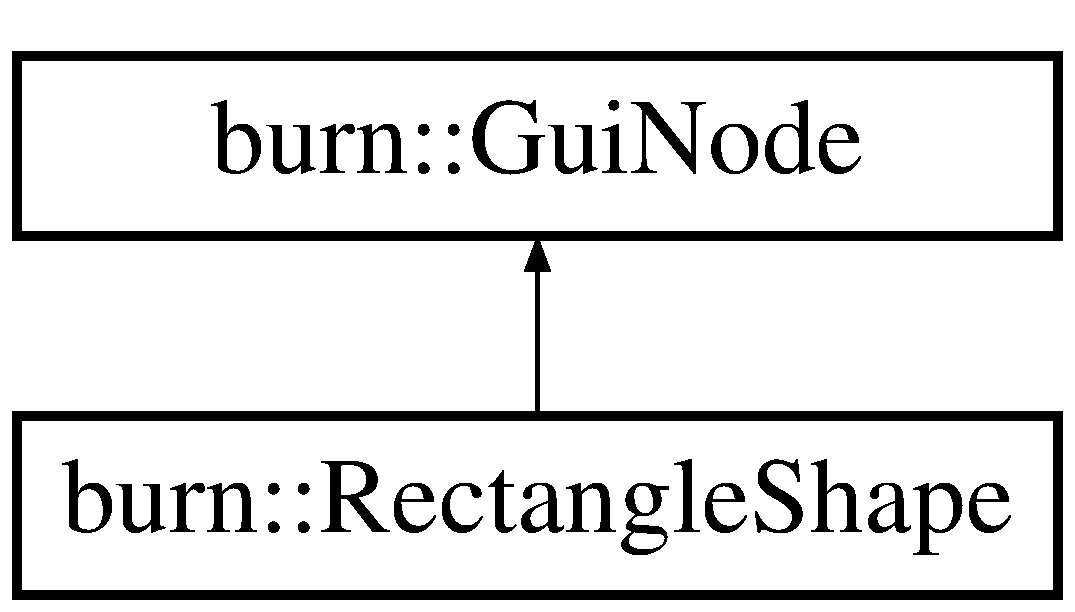
\includegraphics[height=2.000000cm]{classburn_1_1_rectangle_shape}
\end{center}
\end{figure}
\subsection*{Public Member Functions}
\begin{DoxyCompactItemize}
\item 
\hyperlink{classburn_1_1_rectangle_shape_ac029444077fab28ac8522df396dabc03}{Rectangle\-Shape} ()
\item 
void \hyperlink{classburn_1_1_rectangle_shape_a7edd436a3f94e40b781d9f29257f8341}{set\-Dimensions} (const \hyperlink{namespaceburn_af5ed9eb70cbf0fb572098ff43e146a0a}{Vector2f} \&dimensions)
\item 
const \hyperlink{namespaceburn_af5ed9eb70cbf0fb572098ff43e146a0a}{Vector2f} \& \hyperlink{classburn_1_1_rectangle_shape_a02cdb5e26dd7e6ae2d2ec7a06cc57e0b}{get\-Dimensions} () const 
\item 
void \hyperlink{classburn_1_1_rectangle_shape_a3dd38ddf8fb06205fd0f788ec68ba784}{set\-Color} (const \hyperlink{namespaceburn_a58a411b9d83c7970518a9250c1c78068}{Vector4f} \&color)
\item 
const \hyperlink{namespaceburn_a58a411b9d83c7970518a9250c1c78068}{Vector4f} \& \hyperlink{classburn_1_1_rectangle_shape_a0c942ba1465548b1ced36863678dba2b}{get\-Color} () const 
\item 
void \hyperlink{classburn_1_1_rectangle_shape_a39c5c1e57ada4a6beb32a84a501baabf}{draw} ()
\end{DoxyCompactItemize}
\subsection*{Additional Inherited Members}


\subsection{Constructor \& Destructor Documentation}
\hypertarget{classburn_1_1_rectangle_shape_ac029444077fab28ac8522df396dabc03}{\index{burn\-::\-Rectangle\-Shape@{burn\-::\-Rectangle\-Shape}!Rectangle\-Shape@{Rectangle\-Shape}}
\index{Rectangle\-Shape@{Rectangle\-Shape}!burn::RectangleShape@{burn\-::\-Rectangle\-Shape}}
\subsubsection[{Rectangle\-Shape}]{\setlength{\rightskip}{0pt plus 5cm}burn\-::\-Rectangle\-Shape\-::\-Rectangle\-Shape (
\begin{DoxyParamCaption}
{}
\end{DoxyParamCaption}
)}}\label{classburn_1_1_rectangle_shape_ac029444077fab28ac8522df396dabc03}


\subsection{Member Function Documentation}
\hypertarget{classburn_1_1_rectangle_shape_a39c5c1e57ada4a6beb32a84a501baabf}{\index{burn\-::\-Rectangle\-Shape@{burn\-::\-Rectangle\-Shape}!draw@{draw}}
\index{draw@{draw}!burn::RectangleShape@{burn\-::\-Rectangle\-Shape}}
\subsubsection[{draw}]{\setlength{\rightskip}{0pt plus 5cm}void burn\-::\-Rectangle\-Shape\-::draw (
\begin{DoxyParamCaption}
{}
\end{DoxyParamCaption}
)\hspace{0.3cm}{\ttfamily [virtual]}}}\label{classburn_1_1_rectangle_shape_a39c5c1e57ada4a6beb32a84a501baabf}


Implements \hyperlink{classburn_1_1_gui_node_ac283552733ae59c4f1b7fa05c79cb517}{burn\-::\-Gui\-Node}.

\hypertarget{classburn_1_1_rectangle_shape_a0c942ba1465548b1ced36863678dba2b}{\index{burn\-::\-Rectangle\-Shape@{burn\-::\-Rectangle\-Shape}!get\-Color@{get\-Color}}
\index{get\-Color@{get\-Color}!burn::RectangleShape@{burn\-::\-Rectangle\-Shape}}
\subsubsection[{get\-Color}]{\setlength{\rightskip}{0pt plus 5cm}const {\bf Vector4f}\& burn\-::\-Rectangle\-Shape\-::get\-Color (
\begin{DoxyParamCaption}
{}
\end{DoxyParamCaption}
) const}}\label{classburn_1_1_rectangle_shape_a0c942ba1465548b1ced36863678dba2b}
\hypertarget{classburn_1_1_rectangle_shape_a02cdb5e26dd7e6ae2d2ec7a06cc57e0b}{\index{burn\-::\-Rectangle\-Shape@{burn\-::\-Rectangle\-Shape}!get\-Dimensions@{get\-Dimensions}}
\index{get\-Dimensions@{get\-Dimensions}!burn::RectangleShape@{burn\-::\-Rectangle\-Shape}}
\subsubsection[{get\-Dimensions}]{\setlength{\rightskip}{0pt plus 5cm}const {\bf Vector2f}\& burn\-::\-Rectangle\-Shape\-::get\-Dimensions (
\begin{DoxyParamCaption}
{}
\end{DoxyParamCaption}
) const}}\label{classburn_1_1_rectangle_shape_a02cdb5e26dd7e6ae2d2ec7a06cc57e0b}
\hypertarget{classburn_1_1_rectangle_shape_a3dd38ddf8fb06205fd0f788ec68ba784}{\index{burn\-::\-Rectangle\-Shape@{burn\-::\-Rectangle\-Shape}!set\-Color@{set\-Color}}
\index{set\-Color@{set\-Color}!burn::RectangleShape@{burn\-::\-Rectangle\-Shape}}
\subsubsection[{set\-Color}]{\setlength{\rightskip}{0pt plus 5cm}void burn\-::\-Rectangle\-Shape\-::set\-Color (
\begin{DoxyParamCaption}
\item[{const {\bf Vector4f} \&}]{color}
\end{DoxyParamCaption}
)}}\label{classburn_1_1_rectangle_shape_a3dd38ddf8fb06205fd0f788ec68ba784}
\hypertarget{classburn_1_1_rectangle_shape_a7edd436a3f94e40b781d9f29257f8341}{\index{burn\-::\-Rectangle\-Shape@{burn\-::\-Rectangle\-Shape}!set\-Dimensions@{set\-Dimensions}}
\index{set\-Dimensions@{set\-Dimensions}!burn::RectangleShape@{burn\-::\-Rectangle\-Shape}}
\subsubsection[{set\-Dimensions}]{\setlength{\rightskip}{0pt plus 5cm}void burn\-::\-Rectangle\-Shape\-::set\-Dimensions (
\begin{DoxyParamCaption}
\item[{const {\bf Vector2f} \&}]{dimensions}
\end{DoxyParamCaption}
)}}\label{classburn_1_1_rectangle_shape_a7edd436a3f94e40b781d9f29257f8341}


The documentation for this class was generated from the following file\-:\begin{DoxyCompactItemize}
\item 
include/\-Burngine/\-Graphics/\-Gui/2\-D/\hyperlink{_rectangle_shape_8h}{Rectangle\-Shape.\-h}\end{DoxyCompactItemize}

\hypertarget{classburn_1_1_render_texture}{\section{burn\-:\-:Render\-Texture Class Reference}
\label{classburn_1_1_render_texture}\index{burn\-::\-Render\-Texture@{burn\-::\-Render\-Texture}}
}


{\ttfamily \#include $<$Render\-Texture.\-h$>$}

Inheritance diagram for burn\-:\-:Render\-Texture\-:\begin{figure}[H]
\begin{center}
\leavevmode
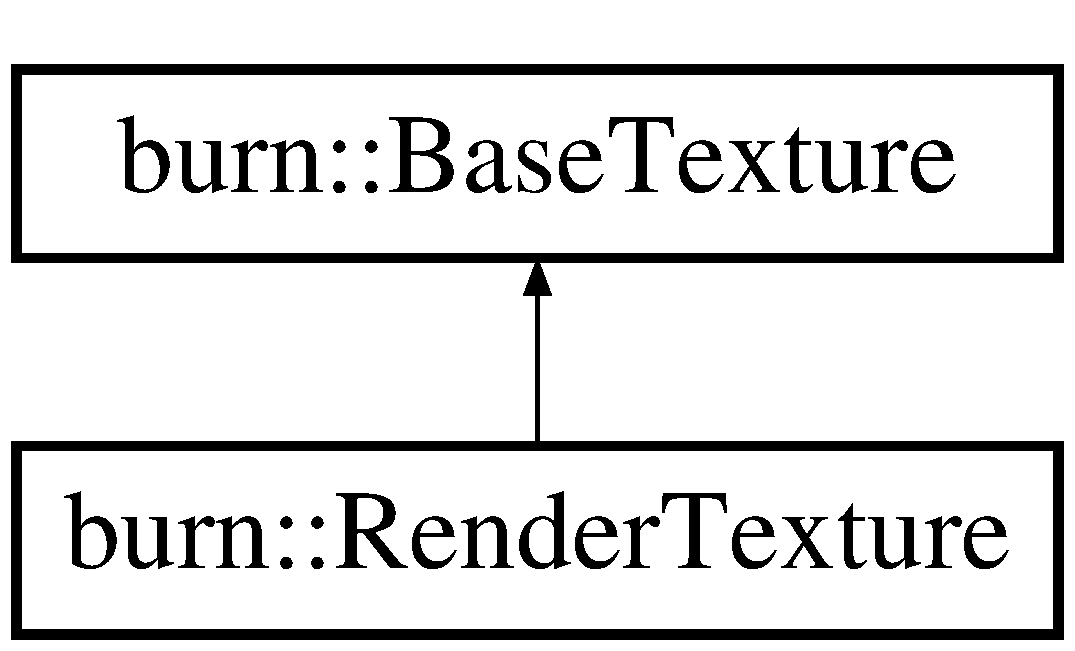
\includegraphics[height=2.000000cm]{classburn_1_1_render_texture}
\end{center}
\end{figure}
\subsection*{Public Member Functions}
\begin{DoxyCompactItemize}
\item 
\hyperlink{classburn_1_1_render_texture_a45a90ff516418ff94aab80a662111bf2}{Render\-Texture} ()
\item 
\hyperlink{classburn_1_1_render_texture_aa4d4ccf9bc258394db5e3c9b17a8240a}{$\sim$\-Render\-Texture} ()
\item 
\hyperlink{classburn_1_1_render_texture_a88571931f632f9a48c2799158dda90c6}{Render\-Texture} (const \hyperlink{classburn_1_1_render_texture}{Render\-Texture} \&other)=delete
\item 
\hyperlink{classburn_1_1_render_texture}{Render\-Texture} \& \hyperlink{classburn_1_1_render_texture_acce2c388ed4850846da563480d2e549c}{operator=} (const \hyperlink{classburn_1_1_render_texture}{Render\-Texture} \&other)=delete
\item 
bool \hyperlink{classburn_1_1_render_texture_afb60cfbc42c0b3fc3543b3d2a954f7dd}{create} (const \hyperlink{namespaceburn_a6805fa33c49c4c3db88a7bebba2c408f}{Vector2ui} \&dimensions)
\item 
void \hyperlink{classburn_1_1_render_texture_a6eb38d6c2e0625a5a369f296598ce64a}{bind\-As\-Target} () const 
\item 
void \hyperlink{classburn_1_1_render_texture_a3316518369cf057633d22d06a6b1b6bb}{clear} () const 
\item 
void \hyperlink{classburn_1_1_render_texture_a80874c4d209be8823dbf9a2e116e6192}{draw\-Fullscreen} ()
\item 
void \hyperlink{classburn_1_1_render_texture_a2f482e794c0c46f56ce89656afe7cefc}{draw} (const \hyperlink{namespaceburn_af5ed9eb70cbf0fb572098ff43e146a0a}{Vector2f} \&position, const \hyperlink{namespaceburn_af5ed9eb70cbf0fb572098ff43e146a0a}{Vector2f} \&size)
\item 
bool \hyperlink{classburn_1_1_render_texture_ac4f8310b46a88a371213f519eb48aa4f}{is\-Created} () const 
\item 
bool \hyperlink{classburn_1_1_render_texture_ac290b3294c10d10628151dc06f15cbb7}{add\-Color\-Attachment} (const G\-Lenum \&attachment)
\end{DoxyCompactItemize}
\subsection*{Additional Inherited Members}


\subsection{Constructor \& Destructor Documentation}
\hypertarget{classburn_1_1_render_texture_a45a90ff516418ff94aab80a662111bf2}{\index{burn\-::\-Render\-Texture@{burn\-::\-Render\-Texture}!Render\-Texture@{Render\-Texture}}
\index{Render\-Texture@{Render\-Texture}!burn::RenderTexture@{burn\-::\-Render\-Texture}}
\subsubsection[{Render\-Texture}]{\setlength{\rightskip}{0pt plus 5cm}burn\-::\-Render\-Texture\-::\-Render\-Texture (
\begin{DoxyParamCaption}
{}
\end{DoxyParamCaption}
)}}\label{classburn_1_1_render_texture_a45a90ff516418ff94aab80a662111bf2}
\hypertarget{classburn_1_1_render_texture_aa4d4ccf9bc258394db5e3c9b17a8240a}{\index{burn\-::\-Render\-Texture@{burn\-::\-Render\-Texture}!$\sim$\-Render\-Texture@{$\sim$\-Render\-Texture}}
\index{$\sim$\-Render\-Texture@{$\sim$\-Render\-Texture}!burn::RenderTexture@{burn\-::\-Render\-Texture}}
\subsubsection[{$\sim$\-Render\-Texture}]{\setlength{\rightskip}{0pt plus 5cm}burn\-::\-Render\-Texture\-::$\sim$\-Render\-Texture (
\begin{DoxyParamCaption}
{}
\end{DoxyParamCaption}
)}}\label{classburn_1_1_render_texture_aa4d4ccf9bc258394db5e3c9b17a8240a}
\hypertarget{classburn_1_1_render_texture_a88571931f632f9a48c2799158dda90c6}{\index{burn\-::\-Render\-Texture@{burn\-::\-Render\-Texture}!Render\-Texture@{Render\-Texture}}
\index{Render\-Texture@{Render\-Texture}!burn::RenderTexture@{burn\-::\-Render\-Texture}}
\subsubsection[{Render\-Texture}]{\setlength{\rightskip}{0pt plus 5cm}burn\-::\-Render\-Texture\-::\-Render\-Texture (
\begin{DoxyParamCaption}
\item[{const {\bf Render\-Texture} \&}]{other}
\end{DoxyParamCaption}
)\hspace{0.3cm}{\ttfamily [delete]}}}\label{classburn_1_1_render_texture_a88571931f632f9a48c2799158dda90c6}


\subsection{Member Function Documentation}
\hypertarget{classburn_1_1_render_texture_ac290b3294c10d10628151dc06f15cbb7}{\index{burn\-::\-Render\-Texture@{burn\-::\-Render\-Texture}!add\-Color\-Attachment@{add\-Color\-Attachment}}
\index{add\-Color\-Attachment@{add\-Color\-Attachment}!burn::RenderTexture@{burn\-::\-Render\-Texture}}
\subsubsection[{add\-Color\-Attachment}]{\setlength{\rightskip}{0pt plus 5cm}bool burn\-::\-Render\-Texture\-::add\-Color\-Attachment (
\begin{DoxyParamCaption}
\item[{const G\-Lenum \&}]{attachment}
\end{DoxyParamCaption}
)}}\label{classburn_1_1_render_texture_ac290b3294c10d10628151dc06f15cbb7}
\hypertarget{classburn_1_1_render_texture_a6eb38d6c2e0625a5a369f296598ce64a}{\index{burn\-::\-Render\-Texture@{burn\-::\-Render\-Texture}!bind\-As\-Target@{bind\-As\-Target}}
\index{bind\-As\-Target@{bind\-As\-Target}!burn::RenderTexture@{burn\-::\-Render\-Texture}}
\subsubsection[{bind\-As\-Target}]{\setlength{\rightskip}{0pt plus 5cm}void burn\-::\-Render\-Texture\-::bind\-As\-Target (
\begin{DoxyParamCaption}
{}
\end{DoxyParamCaption}
) const}}\label{classburn_1_1_render_texture_a6eb38d6c2e0625a5a369f296598ce64a}
\hypertarget{classburn_1_1_render_texture_a3316518369cf057633d22d06a6b1b6bb}{\index{burn\-::\-Render\-Texture@{burn\-::\-Render\-Texture}!clear@{clear}}
\index{clear@{clear}!burn::RenderTexture@{burn\-::\-Render\-Texture}}
\subsubsection[{clear}]{\setlength{\rightskip}{0pt plus 5cm}void burn\-::\-Render\-Texture\-::clear (
\begin{DoxyParamCaption}
{}
\end{DoxyParamCaption}
) const}}\label{classburn_1_1_render_texture_a3316518369cf057633d22d06a6b1b6bb}
\hypertarget{classburn_1_1_render_texture_afb60cfbc42c0b3fc3543b3d2a954f7dd}{\index{burn\-::\-Render\-Texture@{burn\-::\-Render\-Texture}!create@{create}}
\index{create@{create}!burn::RenderTexture@{burn\-::\-Render\-Texture}}
\subsubsection[{create}]{\setlength{\rightskip}{0pt plus 5cm}bool burn\-::\-Render\-Texture\-::create (
\begin{DoxyParamCaption}
\item[{const {\bf Vector2ui} \&}]{dimensions}
\end{DoxyParamCaption}
)}}\label{classburn_1_1_render_texture_afb60cfbc42c0b3fc3543b3d2a954f7dd}
\hypertarget{classburn_1_1_render_texture_a2f482e794c0c46f56ce89656afe7cefc}{\index{burn\-::\-Render\-Texture@{burn\-::\-Render\-Texture}!draw@{draw}}
\index{draw@{draw}!burn::RenderTexture@{burn\-::\-Render\-Texture}}
\subsubsection[{draw}]{\setlength{\rightskip}{0pt plus 5cm}void burn\-::\-Render\-Texture\-::draw (
\begin{DoxyParamCaption}
\item[{const {\bf Vector2f} \&}]{position, }
\item[{const {\bf Vector2f} \&}]{size}
\end{DoxyParamCaption}
)}}\label{classburn_1_1_render_texture_a2f482e794c0c46f56ce89656afe7cefc}
\hypertarget{classburn_1_1_render_texture_a80874c4d209be8823dbf9a2e116e6192}{\index{burn\-::\-Render\-Texture@{burn\-::\-Render\-Texture}!draw\-Fullscreen@{draw\-Fullscreen}}
\index{draw\-Fullscreen@{draw\-Fullscreen}!burn::RenderTexture@{burn\-::\-Render\-Texture}}
\subsubsection[{draw\-Fullscreen}]{\setlength{\rightskip}{0pt plus 5cm}void burn\-::\-Render\-Texture\-::draw\-Fullscreen (
\begin{DoxyParamCaption}
{}
\end{DoxyParamCaption}
)}}\label{classburn_1_1_render_texture_a80874c4d209be8823dbf9a2e116e6192}
\hypertarget{classburn_1_1_render_texture_ac4f8310b46a88a371213f519eb48aa4f}{\index{burn\-::\-Render\-Texture@{burn\-::\-Render\-Texture}!is\-Created@{is\-Created}}
\index{is\-Created@{is\-Created}!burn::RenderTexture@{burn\-::\-Render\-Texture}}
\subsubsection[{is\-Created}]{\setlength{\rightskip}{0pt plus 5cm}bool burn\-::\-Render\-Texture\-::is\-Created (
\begin{DoxyParamCaption}
{}
\end{DoxyParamCaption}
) const}}\label{classburn_1_1_render_texture_ac4f8310b46a88a371213f519eb48aa4f}
\hypertarget{classburn_1_1_render_texture_acce2c388ed4850846da563480d2e549c}{\index{burn\-::\-Render\-Texture@{burn\-::\-Render\-Texture}!operator=@{operator=}}
\index{operator=@{operator=}!burn::RenderTexture@{burn\-::\-Render\-Texture}}
\subsubsection[{operator=}]{\setlength{\rightskip}{0pt plus 5cm}{\bf Render\-Texture}\& burn\-::\-Render\-Texture\-::operator= (
\begin{DoxyParamCaption}
\item[{const {\bf Render\-Texture} \&}]{other}
\end{DoxyParamCaption}
)\hspace{0.3cm}{\ttfamily [delete]}}}\label{classburn_1_1_render_texture_acce2c388ed4850846da563480d2e549c}


The documentation for this class was generated from the following file\-:\begin{DoxyCompactItemize}
\item 
include/\-Burngine/\-Graphics/\-Texture/\hyperlink{_render_texture_8h}{Render\-Texture.\-h}\end{DoxyCompactItemize}

\hypertarget{classburn_1_1_reporter}{\section{burn\-:\-:Reporter Class Reference}
\label{classburn_1_1_reporter}\index{burn\-::\-Reporter@{burn\-::\-Reporter}}
}


{\ttfamily \#include $<$Reporter.\-h$>$}

\subsection*{Public Types}
\begin{DoxyCompactItemize}
\item 
enum \hyperlink{classburn_1_1_reporter_a854e2c1c171ee6de2235efb5d7e8a3c7}{Message\-Type} \{ \hyperlink{classburn_1_1_reporter_a854e2c1c171ee6de2235efb5d7e8a3c7ab81a578256e642de89288137305fc594}{N\-O\-T\-I\-F\-I\-C\-A\-T\-I\-O\-N} = 0, 
\hyperlink{classburn_1_1_reporter_a854e2c1c171ee6de2235efb5d7e8a3c7afe916dc9c0a7ff642a4c0b7dee098ee6}{W\-A\-R\-N\-I\-N\-G}, 
\hyperlink{classburn_1_1_reporter_a854e2c1c171ee6de2235efb5d7e8a3c7a5cd98b46038b6310aeb15c06c9e9b7ac}{E\-R\-R\-O\-R}
 \}
\end{DoxyCompactItemize}
\subsection*{Public Member Functions}
\begin{DoxyCompactItemize}
\item 
\hyperlink{classburn_1_1_reporter_a4845e294015558d7965121455d7be5a8}{Reporter} ()=delete
\begin{DoxyCompactList}\small\item\em \hyperlink{classburn_1_1_reporter}{Reporter} is a static class. \end{DoxyCompactList}\end{DoxyCompactItemize}
\subsection*{Static Public Member Functions}
\begin{DoxyCompactItemize}
\item 
static void \hyperlink{classburn_1_1_reporter_aed47a1d0dd9cfd4bf6706a9e470e338d}{report} (const std\-::string \&message, const \hyperlink{classburn_1_1_reporter_a854e2c1c171ee6de2235efb5d7e8a3c7}{Message\-Type} \&type=\hyperlink{classburn_1_1_reporter_a854e2c1c171ee6de2235efb5d7e8a3c7ab81a578256e642de89288137305fc594}{N\-O\-T\-I\-F\-I\-C\-A\-T\-I\-O\-N})
\end{DoxyCompactItemize}


\subsection{Member Enumeration Documentation}
\hypertarget{classburn_1_1_reporter_a854e2c1c171ee6de2235efb5d7e8a3c7}{\index{burn\-::\-Reporter@{burn\-::\-Reporter}!Message\-Type@{Message\-Type}}
\index{Message\-Type@{Message\-Type}!burn::Reporter@{burn\-::\-Reporter}}
\subsubsection[{Message\-Type}]{\setlength{\rightskip}{0pt plus 5cm}enum {\bf burn\-::\-Reporter\-::\-Message\-Type}}}\label{classburn_1_1_reporter_a854e2c1c171ee6de2235efb5d7e8a3c7}
\begin{Desc}
\item[Enumerator]\par
\begin{description}
\index{N\-O\-T\-I\-F\-I\-C\-A\-T\-I\-O\-N@{N\-O\-T\-I\-F\-I\-C\-A\-T\-I\-O\-N}!burn\-::\-Reporter@{burn\-::\-Reporter}}\index{burn\-::\-Reporter@{burn\-::\-Reporter}!N\-O\-T\-I\-F\-I\-C\-A\-T\-I\-O\-N@{N\-O\-T\-I\-F\-I\-C\-A\-T\-I\-O\-N}}\item[{\em 
\hypertarget{classburn_1_1_reporter_a854e2c1c171ee6de2235efb5d7e8a3c7ab81a578256e642de89288137305fc594}{N\-O\-T\-I\-F\-I\-C\-A\-T\-I\-O\-N}\label{classburn_1_1_reporter_a854e2c1c171ee6de2235efb5d7e8a3c7ab81a578256e642de89288137305fc594}
}]\index{W\-A\-R\-N\-I\-N\-G@{W\-A\-R\-N\-I\-N\-G}!burn\-::\-Reporter@{burn\-::\-Reporter}}\index{burn\-::\-Reporter@{burn\-::\-Reporter}!W\-A\-R\-N\-I\-N\-G@{W\-A\-R\-N\-I\-N\-G}}\item[{\em 
\hypertarget{classburn_1_1_reporter_a854e2c1c171ee6de2235efb5d7e8a3c7afe916dc9c0a7ff642a4c0b7dee098ee6}{W\-A\-R\-N\-I\-N\-G}\label{classburn_1_1_reporter_a854e2c1c171ee6de2235efb5d7e8a3c7afe916dc9c0a7ff642a4c0b7dee098ee6}
}]\index{E\-R\-R\-O\-R@{E\-R\-R\-O\-R}!burn\-::\-Reporter@{burn\-::\-Reporter}}\index{burn\-::\-Reporter@{burn\-::\-Reporter}!E\-R\-R\-O\-R@{E\-R\-R\-O\-R}}\item[{\em 
\hypertarget{classburn_1_1_reporter_a854e2c1c171ee6de2235efb5d7e8a3c7a5cd98b46038b6310aeb15c06c9e9b7ac}{E\-R\-R\-O\-R}\label{classburn_1_1_reporter_a854e2c1c171ee6de2235efb5d7e8a3c7a5cd98b46038b6310aeb15c06c9e9b7ac}
}]\end{description}
\end{Desc}


\subsection{Constructor \& Destructor Documentation}
\hypertarget{classburn_1_1_reporter_a4845e294015558d7965121455d7be5a8}{\index{burn\-::\-Reporter@{burn\-::\-Reporter}!Reporter@{Reporter}}
\index{Reporter@{Reporter}!burn::Reporter@{burn\-::\-Reporter}}
\subsubsection[{Reporter}]{\setlength{\rightskip}{0pt plus 5cm}burn\-::\-Reporter\-::\-Reporter (
\begin{DoxyParamCaption}
{}
\end{DoxyParamCaption}
)\hspace{0.3cm}{\ttfamily [delete]}}}\label{classburn_1_1_reporter_a4845e294015558d7965121455d7be5a8}


\hyperlink{classburn_1_1_reporter}{Reporter} is a static class. 



\subsection{Member Function Documentation}
\hypertarget{classburn_1_1_reporter_aed47a1d0dd9cfd4bf6706a9e470e338d}{\index{burn\-::\-Reporter@{burn\-::\-Reporter}!report@{report}}
\index{report@{report}!burn::Reporter@{burn\-::\-Reporter}}
\subsubsection[{report}]{\setlength{\rightskip}{0pt plus 5cm}static void burn\-::\-Reporter\-::report (
\begin{DoxyParamCaption}
\item[{const std\-::string \&}]{message, }
\item[{const {\bf Message\-Type} \&}]{type = {\ttfamily {\bf N\-O\-T\-I\-F\-I\-C\-A\-T\-I\-O\-N}}}
\end{DoxyParamCaption}
)\hspace{0.3cm}{\ttfamily [static]}}}\label{classburn_1_1_reporter_aed47a1d0dd9cfd4bf6706a9e470e338d}


The documentation for this class was generated from the following file\-:\begin{DoxyCompactItemize}
\item 
include/\-Burngine/\-System/\hyperlink{_reporter_8h}{Reporter.\-h}\end{DoxyCompactItemize}

\hypertarget{classburn_1_1_sampler}{\section{burn\-:\-:Sampler Class Reference}
\label{classburn_1_1_sampler}\index{burn\-::\-Sampler@{burn\-::\-Sampler}}
}


{\ttfamily \#include $<$Sampler.\-h$>$}

\subsection*{Public Types}
\begin{DoxyCompactItemize}
\item 
enum \hyperlink{classburn_1_1_sampler_a09433eae16f8623591d415a3f8c6afec}{Magnification\-Filtering} \{ \hyperlink{classburn_1_1_sampler_a09433eae16f8623591d415a3f8c6afeca686313d0b445f86b99fc81ca846d106f}{M\-A\-G\-\_\-\-N\-E\-A\-R\-E\-S\-T}, 
\hyperlink{classburn_1_1_sampler_a09433eae16f8623591d415a3f8c6afecad578e8d60f86e9d2189a318edc5c39aa}{M\-A\-G\-\_\-\-B\-I\-L\-I\-N\-E\-A\-R}
 \}
\item 
enum \hyperlink{classburn_1_1_sampler_a09d6e36f45577a56ce230549aeaaab10}{Minification\-Filtering} \{ \\*
\hyperlink{classburn_1_1_sampler_a09d6e36f45577a56ce230549aeaaab10a61c7cb4ef3f10c21b6b085d1872f38f6}{M\-I\-N\-\_\-\-N\-E\-A\-R\-E\-S\-T}, 
\hyperlink{classburn_1_1_sampler_a09d6e36f45577a56ce230549aeaaab10a47e352b7d042db353d893235313d966f}{M\-I\-N\-\_\-\-B\-I\-L\-I\-N\-E\-A\-R}, 
\hyperlink{classburn_1_1_sampler_a09d6e36f45577a56ce230549aeaaab10a117a2dc8277823c30ae52ea0b6382009}{M\-I\-N\-\_\-\-T\-R\-I\-L\-I\-N\-E\-A\-R}, 
\hyperlink{classburn_1_1_sampler_a09d6e36f45577a56ce230549aeaaab10ad73bad33e321c29883fb10d992d96b7b}{M\-I\-N\-\_\-\-N\-E\-A\-R\-E\-S\-T\-\_\-\-M\-I\-P\-M\-A\-P}, 
\\*
\hyperlink{classburn_1_1_sampler_a09d6e36f45577a56ce230549aeaaab10ab216362260b08920589fc442fa021e32}{M\-I\-N\-\_\-\-B\-I\-L\-I\-N\-E\-A\-R\-\_\-\-M\-I\-P\-M\-A\-P}
 \}
\end{DoxyCompactItemize}
\subsection*{Public Member Functions}
\begin{DoxyCompactItemize}
\item 
\hyperlink{classburn_1_1_sampler_a480b4acfd17dd57a0c121bb5ebe3d656}{Sampler} ()
\item 
\hyperlink{classburn_1_1_sampler_a738307fd709142b1a44e0c6a035ddafa}{Sampler} (const \hyperlink{classburn_1_1_sampler}{Sampler} \&other)
\item 
\hyperlink{classburn_1_1_sampler}{Sampler} \& \hyperlink{classburn_1_1_sampler_a701aaca7ccac75a4dba5b495c9ed8858}{operator=} (const \hyperlink{classburn_1_1_sampler}{Sampler} \&other)
\item 
\hyperlink{classburn_1_1_sampler_ab5f62848d71b5b270430d746c7d8331c}{$\sim$\-Sampler} ()
\item 
bool \hyperlink{classburn_1_1_sampler_ac71624331b97e00c64a0ef51dd16e06f}{create} ()
\item 
void \hyperlink{classburn_1_1_sampler_adad5b4e01539c026b9dca3cb69b5d85e}{destroy} ()
\item 
bool \hyperlink{classburn_1_1_sampler_a74e374b64020a7d2f682b2a7c5e6c698}{is\-Created} () const 
\item 
void \hyperlink{classburn_1_1_sampler_a0afeda41b62a6cb24194036f6476682f}{bind} (const unsigned int \&unit=0) const 
\item 
bool \hyperlink{classburn_1_1_sampler_a514d577016bec1680d0bbfb4cb60c89e}{set\-Filtering} (const \hyperlink{classburn_1_1_sampler_a09433eae16f8623591d415a3f8c6afec}{Magnification\-Filtering} \&mag, const \hyperlink{classburn_1_1_sampler_a09d6e36f45577a56ce230549aeaaab10}{Minification\-Filtering} \&min)
\item 
bool \hyperlink{classburn_1_1_sampler_a6b4d9dc71c000456eb17409338248fed}{set\-Sampler\-Parameter} (G\-Lenum parameter, G\-Lenum value)
\item 
bool \hyperlink{classburn_1_1_sampler_ae78e2a3cdad25f52ce5683659b7215b1}{set\-Anisotropic\-Level} (const G\-Lfloat \&level)
\item 
const G\-Lfloat \& \hyperlink{classburn_1_1_sampler_ac89ac6da7f36d70d2adeb055a995e51b}{get\-Anisotropic\-Level} () const 
\end{DoxyCompactItemize}
\subsection*{Static Public Member Functions}
\begin{DoxyCompactItemize}
\item 
static void \hyperlink{classburn_1_1_sampler_a4f188f32a1a99deb15784b76a5e90121}{unbind} (const unsigned int \&unit=0)
\end{DoxyCompactItemize}


\subsection{Member Enumeration Documentation}
\hypertarget{classburn_1_1_sampler_a09433eae16f8623591d415a3f8c6afec}{\index{burn\-::\-Sampler@{burn\-::\-Sampler}!Magnification\-Filtering@{Magnification\-Filtering}}
\index{Magnification\-Filtering@{Magnification\-Filtering}!burn::Sampler@{burn\-::\-Sampler}}
\subsubsection[{Magnification\-Filtering}]{\setlength{\rightskip}{0pt plus 5cm}enum {\bf burn\-::\-Sampler\-::\-Magnification\-Filtering}}}\label{classburn_1_1_sampler_a09433eae16f8623591d415a3f8c6afec}
\begin{Desc}
\item[Enumerator]\par
\begin{description}
\index{M\-A\-G\-\_\-\-N\-E\-A\-R\-E\-S\-T@{M\-A\-G\-\_\-\-N\-E\-A\-R\-E\-S\-T}!burn\-::\-Sampler@{burn\-::\-Sampler}}\index{burn\-::\-Sampler@{burn\-::\-Sampler}!M\-A\-G\-\_\-\-N\-E\-A\-R\-E\-S\-T@{M\-A\-G\-\_\-\-N\-E\-A\-R\-E\-S\-T}}\item[{\em 
\hypertarget{classburn_1_1_sampler_a09433eae16f8623591d415a3f8c6afeca686313d0b445f86b99fc81ca846d106f}{M\-A\-G\-\_\-\-N\-E\-A\-R\-E\-S\-T}\label{classburn_1_1_sampler_a09433eae16f8623591d415a3f8c6afeca686313d0b445f86b99fc81ca846d106f}
}]\index{M\-A\-G\-\_\-\-B\-I\-L\-I\-N\-E\-A\-R@{M\-A\-G\-\_\-\-B\-I\-L\-I\-N\-E\-A\-R}!burn\-::\-Sampler@{burn\-::\-Sampler}}\index{burn\-::\-Sampler@{burn\-::\-Sampler}!M\-A\-G\-\_\-\-B\-I\-L\-I\-N\-E\-A\-R@{M\-A\-G\-\_\-\-B\-I\-L\-I\-N\-E\-A\-R}}\item[{\em 
\hypertarget{classburn_1_1_sampler_a09433eae16f8623591d415a3f8c6afecad578e8d60f86e9d2189a318edc5c39aa}{M\-A\-G\-\_\-\-B\-I\-L\-I\-N\-E\-A\-R}\label{classburn_1_1_sampler_a09433eae16f8623591d415a3f8c6afecad578e8d60f86e9d2189a318edc5c39aa}
}]\end{description}
\end{Desc}
\hypertarget{classburn_1_1_sampler_a09d6e36f45577a56ce230549aeaaab10}{\index{burn\-::\-Sampler@{burn\-::\-Sampler}!Minification\-Filtering@{Minification\-Filtering}}
\index{Minification\-Filtering@{Minification\-Filtering}!burn::Sampler@{burn\-::\-Sampler}}
\subsubsection[{Minification\-Filtering}]{\setlength{\rightskip}{0pt plus 5cm}enum {\bf burn\-::\-Sampler\-::\-Minification\-Filtering}}}\label{classburn_1_1_sampler_a09d6e36f45577a56ce230549aeaaab10}
\begin{Desc}
\item[Enumerator]\par
\begin{description}
\index{M\-I\-N\-\_\-\-N\-E\-A\-R\-E\-S\-T@{M\-I\-N\-\_\-\-N\-E\-A\-R\-E\-S\-T}!burn\-::\-Sampler@{burn\-::\-Sampler}}\index{burn\-::\-Sampler@{burn\-::\-Sampler}!M\-I\-N\-\_\-\-N\-E\-A\-R\-E\-S\-T@{M\-I\-N\-\_\-\-N\-E\-A\-R\-E\-S\-T}}\item[{\em 
\hypertarget{classburn_1_1_sampler_a09d6e36f45577a56ce230549aeaaab10a61c7cb4ef3f10c21b6b085d1872f38f6}{M\-I\-N\-\_\-\-N\-E\-A\-R\-E\-S\-T}\label{classburn_1_1_sampler_a09d6e36f45577a56ce230549aeaaab10a61c7cb4ef3f10c21b6b085d1872f38f6}
}]\index{M\-I\-N\-\_\-\-B\-I\-L\-I\-N\-E\-A\-R@{M\-I\-N\-\_\-\-B\-I\-L\-I\-N\-E\-A\-R}!burn\-::\-Sampler@{burn\-::\-Sampler}}\index{burn\-::\-Sampler@{burn\-::\-Sampler}!M\-I\-N\-\_\-\-B\-I\-L\-I\-N\-E\-A\-R@{M\-I\-N\-\_\-\-B\-I\-L\-I\-N\-E\-A\-R}}\item[{\em 
\hypertarget{classburn_1_1_sampler_a09d6e36f45577a56ce230549aeaaab10a47e352b7d042db353d893235313d966f}{M\-I\-N\-\_\-\-B\-I\-L\-I\-N\-E\-A\-R}\label{classburn_1_1_sampler_a09d6e36f45577a56ce230549aeaaab10a47e352b7d042db353d893235313d966f}
}]\index{M\-I\-N\-\_\-\-T\-R\-I\-L\-I\-N\-E\-A\-R@{M\-I\-N\-\_\-\-T\-R\-I\-L\-I\-N\-E\-A\-R}!burn\-::\-Sampler@{burn\-::\-Sampler}}\index{burn\-::\-Sampler@{burn\-::\-Sampler}!M\-I\-N\-\_\-\-T\-R\-I\-L\-I\-N\-E\-A\-R@{M\-I\-N\-\_\-\-T\-R\-I\-L\-I\-N\-E\-A\-R}}\item[{\em 
\hypertarget{classburn_1_1_sampler_a09d6e36f45577a56ce230549aeaaab10a117a2dc8277823c30ae52ea0b6382009}{M\-I\-N\-\_\-\-T\-R\-I\-L\-I\-N\-E\-A\-R}\label{classburn_1_1_sampler_a09d6e36f45577a56ce230549aeaaab10a117a2dc8277823c30ae52ea0b6382009}
}]\index{M\-I\-N\-\_\-\-N\-E\-A\-R\-E\-S\-T\-\_\-\-M\-I\-P\-M\-A\-P@{M\-I\-N\-\_\-\-N\-E\-A\-R\-E\-S\-T\-\_\-\-M\-I\-P\-M\-A\-P}!burn\-::\-Sampler@{burn\-::\-Sampler}}\index{burn\-::\-Sampler@{burn\-::\-Sampler}!M\-I\-N\-\_\-\-N\-E\-A\-R\-E\-S\-T\-\_\-\-M\-I\-P\-M\-A\-P@{M\-I\-N\-\_\-\-N\-E\-A\-R\-E\-S\-T\-\_\-\-M\-I\-P\-M\-A\-P}}\item[{\em 
\hypertarget{classburn_1_1_sampler_a09d6e36f45577a56ce230549aeaaab10ad73bad33e321c29883fb10d992d96b7b}{M\-I\-N\-\_\-\-N\-E\-A\-R\-E\-S\-T\-\_\-\-M\-I\-P\-M\-A\-P}\label{classburn_1_1_sampler_a09d6e36f45577a56ce230549aeaaab10ad73bad33e321c29883fb10d992d96b7b}
}]\index{M\-I\-N\-\_\-\-B\-I\-L\-I\-N\-E\-A\-R\-\_\-\-M\-I\-P\-M\-A\-P@{M\-I\-N\-\_\-\-B\-I\-L\-I\-N\-E\-A\-R\-\_\-\-M\-I\-P\-M\-A\-P}!burn\-::\-Sampler@{burn\-::\-Sampler}}\index{burn\-::\-Sampler@{burn\-::\-Sampler}!M\-I\-N\-\_\-\-B\-I\-L\-I\-N\-E\-A\-R\-\_\-\-M\-I\-P\-M\-A\-P@{M\-I\-N\-\_\-\-B\-I\-L\-I\-N\-E\-A\-R\-\_\-\-M\-I\-P\-M\-A\-P}}\item[{\em 
\hypertarget{classburn_1_1_sampler_a09d6e36f45577a56ce230549aeaaab10ab216362260b08920589fc442fa021e32}{M\-I\-N\-\_\-\-B\-I\-L\-I\-N\-E\-A\-R\-\_\-\-M\-I\-P\-M\-A\-P}\label{classburn_1_1_sampler_a09d6e36f45577a56ce230549aeaaab10ab216362260b08920589fc442fa021e32}
}]\end{description}
\end{Desc}


\subsection{Constructor \& Destructor Documentation}
\hypertarget{classburn_1_1_sampler_a480b4acfd17dd57a0c121bb5ebe3d656}{\index{burn\-::\-Sampler@{burn\-::\-Sampler}!Sampler@{Sampler}}
\index{Sampler@{Sampler}!burn::Sampler@{burn\-::\-Sampler}}
\subsubsection[{Sampler}]{\setlength{\rightskip}{0pt plus 5cm}burn\-::\-Sampler\-::\-Sampler (
\begin{DoxyParamCaption}
{}
\end{DoxyParamCaption}
)}}\label{classburn_1_1_sampler_a480b4acfd17dd57a0c121bb5ebe3d656}
\hypertarget{classburn_1_1_sampler_a738307fd709142b1a44e0c6a035ddafa}{\index{burn\-::\-Sampler@{burn\-::\-Sampler}!Sampler@{Sampler}}
\index{Sampler@{Sampler}!burn::Sampler@{burn\-::\-Sampler}}
\subsubsection[{Sampler}]{\setlength{\rightskip}{0pt plus 5cm}burn\-::\-Sampler\-::\-Sampler (
\begin{DoxyParamCaption}
\item[{const {\bf Sampler} \&}]{other}
\end{DoxyParamCaption}
)}}\label{classburn_1_1_sampler_a738307fd709142b1a44e0c6a035ddafa}
\hypertarget{classburn_1_1_sampler_ab5f62848d71b5b270430d746c7d8331c}{\index{burn\-::\-Sampler@{burn\-::\-Sampler}!$\sim$\-Sampler@{$\sim$\-Sampler}}
\index{$\sim$\-Sampler@{$\sim$\-Sampler}!burn::Sampler@{burn\-::\-Sampler}}
\subsubsection[{$\sim$\-Sampler}]{\setlength{\rightskip}{0pt plus 5cm}burn\-::\-Sampler\-::$\sim$\-Sampler (
\begin{DoxyParamCaption}
{}
\end{DoxyParamCaption}
)}}\label{classburn_1_1_sampler_ab5f62848d71b5b270430d746c7d8331c}


\subsection{Member Function Documentation}
\hypertarget{classburn_1_1_sampler_a0afeda41b62a6cb24194036f6476682f}{\index{burn\-::\-Sampler@{burn\-::\-Sampler}!bind@{bind}}
\index{bind@{bind}!burn::Sampler@{burn\-::\-Sampler}}
\subsubsection[{bind}]{\setlength{\rightskip}{0pt plus 5cm}void burn\-::\-Sampler\-::bind (
\begin{DoxyParamCaption}
\item[{const unsigned int \&}]{unit = {\ttfamily 0}}
\end{DoxyParamCaption}
) const}}\label{classburn_1_1_sampler_a0afeda41b62a6cb24194036f6476682f}
\hypertarget{classburn_1_1_sampler_ac71624331b97e00c64a0ef51dd16e06f}{\index{burn\-::\-Sampler@{burn\-::\-Sampler}!create@{create}}
\index{create@{create}!burn::Sampler@{burn\-::\-Sampler}}
\subsubsection[{create}]{\setlength{\rightskip}{0pt plus 5cm}bool burn\-::\-Sampler\-::create (
\begin{DoxyParamCaption}
{}
\end{DoxyParamCaption}
)}}\label{classburn_1_1_sampler_ac71624331b97e00c64a0ef51dd16e06f}
\hypertarget{classburn_1_1_sampler_adad5b4e01539c026b9dca3cb69b5d85e}{\index{burn\-::\-Sampler@{burn\-::\-Sampler}!destroy@{destroy}}
\index{destroy@{destroy}!burn::Sampler@{burn\-::\-Sampler}}
\subsubsection[{destroy}]{\setlength{\rightskip}{0pt plus 5cm}void burn\-::\-Sampler\-::destroy (
\begin{DoxyParamCaption}
{}
\end{DoxyParamCaption}
)}}\label{classburn_1_1_sampler_adad5b4e01539c026b9dca3cb69b5d85e}
\hypertarget{classburn_1_1_sampler_ac89ac6da7f36d70d2adeb055a995e51b}{\index{burn\-::\-Sampler@{burn\-::\-Sampler}!get\-Anisotropic\-Level@{get\-Anisotropic\-Level}}
\index{get\-Anisotropic\-Level@{get\-Anisotropic\-Level}!burn::Sampler@{burn\-::\-Sampler}}
\subsubsection[{get\-Anisotropic\-Level}]{\setlength{\rightskip}{0pt plus 5cm}const G\-Lfloat\& burn\-::\-Sampler\-::get\-Anisotropic\-Level (
\begin{DoxyParamCaption}
{}
\end{DoxyParamCaption}
) const}}\label{classburn_1_1_sampler_ac89ac6da7f36d70d2adeb055a995e51b}
\hypertarget{classburn_1_1_sampler_a74e374b64020a7d2f682b2a7c5e6c698}{\index{burn\-::\-Sampler@{burn\-::\-Sampler}!is\-Created@{is\-Created}}
\index{is\-Created@{is\-Created}!burn::Sampler@{burn\-::\-Sampler}}
\subsubsection[{is\-Created}]{\setlength{\rightskip}{0pt plus 5cm}bool burn\-::\-Sampler\-::is\-Created (
\begin{DoxyParamCaption}
{}
\end{DoxyParamCaption}
) const}}\label{classburn_1_1_sampler_a74e374b64020a7d2f682b2a7c5e6c698}
\hypertarget{classburn_1_1_sampler_a701aaca7ccac75a4dba5b495c9ed8858}{\index{burn\-::\-Sampler@{burn\-::\-Sampler}!operator=@{operator=}}
\index{operator=@{operator=}!burn::Sampler@{burn\-::\-Sampler}}
\subsubsection[{operator=}]{\setlength{\rightskip}{0pt plus 5cm}{\bf Sampler}\& burn\-::\-Sampler\-::operator= (
\begin{DoxyParamCaption}
\item[{const {\bf Sampler} \&}]{other}
\end{DoxyParamCaption}
)}}\label{classburn_1_1_sampler_a701aaca7ccac75a4dba5b495c9ed8858}
\hypertarget{classburn_1_1_sampler_ae78e2a3cdad25f52ce5683659b7215b1}{\index{burn\-::\-Sampler@{burn\-::\-Sampler}!set\-Anisotropic\-Level@{set\-Anisotropic\-Level}}
\index{set\-Anisotropic\-Level@{set\-Anisotropic\-Level}!burn::Sampler@{burn\-::\-Sampler}}
\subsubsection[{set\-Anisotropic\-Level}]{\setlength{\rightskip}{0pt plus 5cm}bool burn\-::\-Sampler\-::set\-Anisotropic\-Level (
\begin{DoxyParamCaption}
\item[{const G\-Lfloat \&}]{level}
\end{DoxyParamCaption}
)}}\label{classburn_1_1_sampler_ae78e2a3cdad25f52ce5683659b7215b1}
\hypertarget{classburn_1_1_sampler_a514d577016bec1680d0bbfb4cb60c89e}{\index{burn\-::\-Sampler@{burn\-::\-Sampler}!set\-Filtering@{set\-Filtering}}
\index{set\-Filtering@{set\-Filtering}!burn::Sampler@{burn\-::\-Sampler}}
\subsubsection[{set\-Filtering}]{\setlength{\rightskip}{0pt plus 5cm}bool burn\-::\-Sampler\-::set\-Filtering (
\begin{DoxyParamCaption}
\item[{const {\bf Magnification\-Filtering} \&}]{mag, }
\item[{const {\bf Minification\-Filtering} \&}]{min}
\end{DoxyParamCaption}
)}}\label{classburn_1_1_sampler_a514d577016bec1680d0bbfb4cb60c89e}
\hypertarget{classburn_1_1_sampler_a6b4d9dc71c000456eb17409338248fed}{\index{burn\-::\-Sampler@{burn\-::\-Sampler}!set\-Sampler\-Parameter@{set\-Sampler\-Parameter}}
\index{set\-Sampler\-Parameter@{set\-Sampler\-Parameter}!burn::Sampler@{burn\-::\-Sampler}}
\subsubsection[{set\-Sampler\-Parameter}]{\setlength{\rightskip}{0pt plus 5cm}bool burn\-::\-Sampler\-::set\-Sampler\-Parameter (
\begin{DoxyParamCaption}
\item[{G\-Lenum}]{parameter, }
\item[{G\-Lenum}]{value}
\end{DoxyParamCaption}
)}}\label{classburn_1_1_sampler_a6b4d9dc71c000456eb17409338248fed}
\hypertarget{classburn_1_1_sampler_a4f188f32a1a99deb15784b76a5e90121}{\index{burn\-::\-Sampler@{burn\-::\-Sampler}!unbind@{unbind}}
\index{unbind@{unbind}!burn::Sampler@{burn\-::\-Sampler}}
\subsubsection[{unbind}]{\setlength{\rightskip}{0pt plus 5cm}static void burn\-::\-Sampler\-::unbind (
\begin{DoxyParamCaption}
\item[{const unsigned int \&}]{unit = {\ttfamily 0}}
\end{DoxyParamCaption}
)\hspace{0.3cm}{\ttfamily [static]}}}\label{classburn_1_1_sampler_a4f188f32a1a99deb15784b76a5e90121}


The documentation for this class was generated from the following file\-:\begin{DoxyCompactItemize}
\item 
include/\-Burngine/\-Graphics/\-Texture/\hyperlink{_sampler_8h}{Sampler.\-h}\end{DoxyCompactItemize}

\hypertarget{classburn_1_1_scene}{\section{burn\-:\-:Scene Class Reference}
\label{classburn_1_1_scene}\index{burn\-::\-Scene@{burn\-::\-Scene}}
}


{\ttfamily \#include $<$Scene.\-h$>$}

\subsection*{Public Types}
\begin{DoxyCompactItemize}
\item 
enum \hyperlink{classburn_1_1_scene_a992349a23199d694dca7b8cbd4957299}{Render\-Modus} \{ \\*
\hyperlink{classburn_1_1_scene_a992349a23199d694dca7b8cbd4957299a9de887ba3d66505de29d661ec0cb0c63}{C\-O\-M\-P\-O\-S\-I\-T\-I\-O\-N}, 
\hyperlink{classburn_1_1_scene_a992349a23199d694dca7b8cbd4957299ac85a19cebcbd9de06a84f792bec68230}{D\-I\-F\-F\-U\-S\-E}, 
\hyperlink{classburn_1_1_scene_a992349a23199d694dca7b8cbd4957299ab2f9ede76e57d852bf0e82b5e3f1bb76}{N\-O\-R\-M\-A\-L\-\_\-\-W\-S}, 
\hyperlink{classburn_1_1_scene_a992349a23199d694dca7b8cbd4957299a8795288c1c09c990d1e3230b2b16261b}{D\-E\-P\-T\-H}, 
\\*
\hyperlink{classburn_1_1_scene_a992349a23199d694dca7b8cbd4957299abf537b9d28f1932ce09a6879e834ec8d}{P\-O\-S\-I\-T\-I\-O\-N\-\_\-\-W\-S}
 \}
\end{DoxyCompactItemize}
\subsection*{Public Member Functions}
\begin{DoxyCompactItemize}
\item 
\hyperlink{classburn_1_1_scene_a14bb493f34a5c489f2460b94698c8f72}{Scene} (const \hyperlink{classburn_1_1_window}{Window} \&parent\-Window)
\begin{DoxyCompactList}\small\item\em The default constructor. \end{DoxyCompactList}\item 
\hyperlink{classburn_1_1_scene_a7722cda0111bd22ca193174326e66924}{$\sim$\-Scene} ()
\begin{DoxyCompactList}\small\item\em The default destructor. When called by e.\-g. deleting the scene it cleans up its data. In other words it deletes all nodes/cameras/etc. it is holding. \end{DoxyCompactList}\item 
void \hyperlink{classburn_1_1_scene_aca5f35cf0478da8ac4bc79975610ed65}{draw} (const \hyperlink{classburn_1_1_camera}{Camera} \&camera, const \hyperlink{classburn_1_1_scene_a992349a23199d694dca7b8cbd4957299}{Render\-Modus} \&modus=\hyperlink{classburn_1_1_scene_a992349a23199d694dca7b8cbd4957299a9de887ba3d66505de29d661ec0cb0c63}{C\-O\-M\-P\-O\-S\-I\-T\-I\-O\-N})
\begin{DoxyCompactList}\small\item\em Draws every \hyperlink{classburn_1_1_scene_node}{Scene\-Node}. \end{DoxyCompactList}\item 
void \hyperlink{classburn_1_1_scene_aa013e68565bda374fa704f816d8e6847}{attach\-Scene\-Node} (\hyperlink{classburn_1_1_scene_node}{Scene\-Node} \&node)
\item 
void \hyperlink{classburn_1_1_scene_a999ba40b417a1074b58c73e837170e51}{detach\-Scene\-Node} (\hyperlink{classburn_1_1_scene_node}{Scene\-Node} \&node)
\item 
void \hyperlink{classburn_1_1_scene_a32378fec20f95d1ed972869e0a4a5b20}{attach\-Light} (\hyperlink{classburn_1_1_light}{Light} \&light)
\item 
void \hyperlink{classburn_1_1_scene_a6e8c366da48a859641a08d82ac4b293d}{detach\-Light} (\hyperlink{classburn_1_1_light}{Light} \&light)
\item 
void \hyperlink{classburn_1_1_scene_a8d4c2bc5288fed85613b59f68e05e96c}{detach\-All} ()
\item 
void \hyperlink{classburn_1_1_scene_ae569a4b21af331b5403ca444d83e4884}{set\-Sky\-Box} (const \hyperlink{classburn_1_1_sky_box}{Sky\-Box} \&sky\-Box)
\item 
void \hyperlink{classburn_1_1_scene_a8bfd8a10ac26bd647b2391ff6c3b4b66}{set\-Ambient\-Color} (const \hyperlink{namespaceburn_afdd7cfb352b9612432faf6947b6fff74}{Vector3f} \&color)
\item 
const \hyperlink{namespaceburn_afdd7cfb352b9612432faf6947b6fff74}{Vector3f} \& \hyperlink{classburn_1_1_scene_a8abbd3b6bb1737c80366d059bbdc1ea5}{get\-Ambient\-Color} () const 
\end{DoxyCompactItemize}


\subsection{Member Enumeration Documentation}
\hypertarget{classburn_1_1_scene_a992349a23199d694dca7b8cbd4957299}{\index{burn\-::\-Scene@{burn\-::\-Scene}!Render\-Modus@{Render\-Modus}}
\index{Render\-Modus@{Render\-Modus}!burn::Scene@{burn\-::\-Scene}}
\subsubsection[{Render\-Modus}]{\setlength{\rightskip}{0pt plus 5cm}enum {\bf burn\-::\-Scene\-::\-Render\-Modus}}}\label{classburn_1_1_scene_a992349a23199d694dca7b8cbd4957299}
\begin{Desc}
\item[Enumerator]\par
\begin{description}
\index{C\-O\-M\-P\-O\-S\-I\-T\-I\-O\-N@{C\-O\-M\-P\-O\-S\-I\-T\-I\-O\-N}!burn\-::\-Scene@{burn\-::\-Scene}}\index{burn\-::\-Scene@{burn\-::\-Scene}!C\-O\-M\-P\-O\-S\-I\-T\-I\-O\-N@{C\-O\-M\-P\-O\-S\-I\-T\-I\-O\-N}}\item[{\em 
\hypertarget{classburn_1_1_scene_a992349a23199d694dca7b8cbd4957299a9de887ba3d66505de29d661ec0cb0c63}{C\-O\-M\-P\-O\-S\-I\-T\-I\-O\-N}\label{classburn_1_1_scene_a992349a23199d694dca7b8cbd4957299a9de887ba3d66505de29d661ec0cb0c63}
}]\index{D\-I\-F\-F\-U\-S\-E@{D\-I\-F\-F\-U\-S\-E}!burn\-::\-Scene@{burn\-::\-Scene}}\index{burn\-::\-Scene@{burn\-::\-Scene}!D\-I\-F\-F\-U\-S\-E@{D\-I\-F\-F\-U\-S\-E}}\item[{\em 
\hypertarget{classburn_1_1_scene_a992349a23199d694dca7b8cbd4957299ac85a19cebcbd9de06a84f792bec68230}{D\-I\-F\-F\-U\-S\-E}\label{classburn_1_1_scene_a992349a23199d694dca7b8cbd4957299ac85a19cebcbd9de06a84f792bec68230}
}]\index{N\-O\-R\-M\-A\-L\-\_\-\-W\-S@{N\-O\-R\-M\-A\-L\-\_\-\-W\-S}!burn\-::\-Scene@{burn\-::\-Scene}}\index{burn\-::\-Scene@{burn\-::\-Scene}!N\-O\-R\-M\-A\-L\-\_\-\-W\-S@{N\-O\-R\-M\-A\-L\-\_\-\-W\-S}}\item[{\em 
\hypertarget{classburn_1_1_scene_a992349a23199d694dca7b8cbd4957299ab2f9ede76e57d852bf0e82b5e3f1bb76}{N\-O\-R\-M\-A\-L\-\_\-\-W\-S}\label{classburn_1_1_scene_a992349a23199d694dca7b8cbd4957299ab2f9ede76e57d852bf0e82b5e3f1bb76}
}]\index{D\-E\-P\-T\-H@{D\-E\-P\-T\-H}!burn\-::\-Scene@{burn\-::\-Scene}}\index{burn\-::\-Scene@{burn\-::\-Scene}!D\-E\-P\-T\-H@{D\-E\-P\-T\-H}}\item[{\em 
\hypertarget{classburn_1_1_scene_a992349a23199d694dca7b8cbd4957299a8795288c1c09c990d1e3230b2b16261b}{D\-E\-P\-T\-H}\label{classburn_1_1_scene_a992349a23199d694dca7b8cbd4957299a8795288c1c09c990d1e3230b2b16261b}
}]\index{P\-O\-S\-I\-T\-I\-O\-N\-\_\-\-W\-S@{P\-O\-S\-I\-T\-I\-O\-N\-\_\-\-W\-S}!burn\-::\-Scene@{burn\-::\-Scene}}\index{burn\-::\-Scene@{burn\-::\-Scene}!P\-O\-S\-I\-T\-I\-O\-N\-\_\-\-W\-S@{P\-O\-S\-I\-T\-I\-O\-N\-\_\-\-W\-S}}\item[{\em 
\hypertarget{classburn_1_1_scene_a992349a23199d694dca7b8cbd4957299abf537b9d28f1932ce09a6879e834ec8d}{P\-O\-S\-I\-T\-I\-O\-N\-\_\-\-W\-S}\label{classburn_1_1_scene_a992349a23199d694dca7b8cbd4957299abf537b9d28f1932ce09a6879e834ec8d}
}]\end{description}
\end{Desc}


\subsection{Constructor \& Destructor Documentation}
\hypertarget{classburn_1_1_scene_a14bb493f34a5c489f2460b94698c8f72}{\index{burn\-::\-Scene@{burn\-::\-Scene}!Scene@{Scene}}
\index{Scene@{Scene}!burn::Scene@{burn\-::\-Scene}}
\subsubsection[{Scene}]{\setlength{\rightskip}{0pt plus 5cm}burn\-::\-Scene\-::\-Scene (
\begin{DoxyParamCaption}
\item[{const {\bf Window} \&}]{parent\-Window}
\end{DoxyParamCaption}
)}}\label{classburn_1_1_scene_a14bb493f34a5c489f2460b94698c8f72}


The default constructor. 

\hypertarget{classburn_1_1_scene_a7722cda0111bd22ca193174326e66924}{\index{burn\-::\-Scene@{burn\-::\-Scene}!$\sim$\-Scene@{$\sim$\-Scene}}
\index{$\sim$\-Scene@{$\sim$\-Scene}!burn::Scene@{burn\-::\-Scene}}
\subsubsection[{$\sim$\-Scene}]{\setlength{\rightskip}{0pt plus 5cm}burn\-::\-Scene\-::$\sim$\-Scene (
\begin{DoxyParamCaption}
{}
\end{DoxyParamCaption}
)}}\label{classburn_1_1_scene_a7722cda0111bd22ca193174326e66924}


The default destructor. When called by e.\-g. deleting the scene it cleans up its data. In other words it deletes all nodes/cameras/etc. it is holding. 



\subsection{Member Function Documentation}
\hypertarget{classburn_1_1_scene_a32378fec20f95d1ed972869e0a4a5b20}{\index{burn\-::\-Scene@{burn\-::\-Scene}!attach\-Light@{attach\-Light}}
\index{attach\-Light@{attach\-Light}!burn::Scene@{burn\-::\-Scene}}
\subsubsection[{attach\-Light}]{\setlength{\rightskip}{0pt plus 5cm}void burn\-::\-Scene\-::attach\-Light (
\begin{DoxyParamCaption}
\item[{{\bf Light} \&}]{light}
\end{DoxyParamCaption}
)}}\label{classburn_1_1_scene_a32378fec20f95d1ed972869e0a4a5b20}
\hypertarget{classburn_1_1_scene_aa013e68565bda374fa704f816d8e6847}{\index{burn\-::\-Scene@{burn\-::\-Scene}!attach\-Scene\-Node@{attach\-Scene\-Node}}
\index{attach\-Scene\-Node@{attach\-Scene\-Node}!burn::Scene@{burn\-::\-Scene}}
\subsubsection[{attach\-Scene\-Node}]{\setlength{\rightskip}{0pt plus 5cm}void burn\-::\-Scene\-::attach\-Scene\-Node (
\begin{DoxyParamCaption}
\item[{{\bf Scene\-Node} \&}]{node}
\end{DoxyParamCaption}
)}}\label{classburn_1_1_scene_aa013e68565bda374fa704f816d8e6847}
\hypertarget{classburn_1_1_scene_a8d4c2bc5288fed85613b59f68e05e96c}{\index{burn\-::\-Scene@{burn\-::\-Scene}!detach\-All@{detach\-All}}
\index{detach\-All@{detach\-All}!burn::Scene@{burn\-::\-Scene}}
\subsubsection[{detach\-All}]{\setlength{\rightskip}{0pt plus 5cm}void burn\-::\-Scene\-::detach\-All (
\begin{DoxyParamCaption}
{}
\end{DoxyParamCaption}
)}}\label{classburn_1_1_scene_a8d4c2bc5288fed85613b59f68e05e96c}
\hypertarget{classburn_1_1_scene_a6e8c366da48a859641a08d82ac4b293d}{\index{burn\-::\-Scene@{burn\-::\-Scene}!detach\-Light@{detach\-Light}}
\index{detach\-Light@{detach\-Light}!burn::Scene@{burn\-::\-Scene}}
\subsubsection[{detach\-Light}]{\setlength{\rightskip}{0pt plus 5cm}void burn\-::\-Scene\-::detach\-Light (
\begin{DoxyParamCaption}
\item[{{\bf Light} \&}]{light}
\end{DoxyParamCaption}
)}}\label{classburn_1_1_scene_a6e8c366da48a859641a08d82ac4b293d}
\hypertarget{classburn_1_1_scene_a999ba40b417a1074b58c73e837170e51}{\index{burn\-::\-Scene@{burn\-::\-Scene}!detach\-Scene\-Node@{detach\-Scene\-Node}}
\index{detach\-Scene\-Node@{detach\-Scene\-Node}!burn::Scene@{burn\-::\-Scene}}
\subsubsection[{detach\-Scene\-Node}]{\setlength{\rightskip}{0pt plus 5cm}void burn\-::\-Scene\-::detach\-Scene\-Node (
\begin{DoxyParamCaption}
\item[{{\bf Scene\-Node} \&}]{node}
\end{DoxyParamCaption}
)}}\label{classburn_1_1_scene_a999ba40b417a1074b58c73e837170e51}
\hypertarget{classburn_1_1_scene_aca5f35cf0478da8ac4bc79975610ed65}{\index{burn\-::\-Scene@{burn\-::\-Scene}!draw@{draw}}
\index{draw@{draw}!burn::Scene@{burn\-::\-Scene}}
\subsubsection[{draw}]{\setlength{\rightskip}{0pt plus 5cm}void burn\-::\-Scene\-::draw (
\begin{DoxyParamCaption}
\item[{const {\bf Camera} \&}]{camera, }
\item[{const {\bf Render\-Modus} \&}]{modus = {\ttfamily {\bf C\-O\-M\-P\-O\-S\-I\-T\-I\-O\-N}}}
\end{DoxyParamCaption}
)}}\label{classburn_1_1_scene_aca5f35cf0478da8ac4bc79975610ed65}


Draws every \hyperlink{classburn_1_1_scene_node}{Scene\-Node}. 


\begin{DoxyParams}{Parameters}
{\em modus} & Choose a g\-Buffer to dump to screen or set to C\-O\-M\-P\-O\-S\-I\-T\-I\-O\-N to see final result \\
\hline
\end{DoxyParams}
\hypertarget{classburn_1_1_scene_a8abbd3b6bb1737c80366d059bbdc1ea5}{\index{burn\-::\-Scene@{burn\-::\-Scene}!get\-Ambient\-Color@{get\-Ambient\-Color}}
\index{get\-Ambient\-Color@{get\-Ambient\-Color}!burn::Scene@{burn\-::\-Scene}}
\subsubsection[{get\-Ambient\-Color}]{\setlength{\rightskip}{0pt plus 5cm}const {\bf Vector3f}\& burn\-::\-Scene\-::get\-Ambient\-Color (
\begin{DoxyParamCaption}
{}
\end{DoxyParamCaption}
) const}}\label{classburn_1_1_scene_a8abbd3b6bb1737c80366d059bbdc1ea5}
\hypertarget{classburn_1_1_scene_a8bfd8a10ac26bd647b2391ff6c3b4b66}{\index{burn\-::\-Scene@{burn\-::\-Scene}!set\-Ambient\-Color@{set\-Ambient\-Color}}
\index{set\-Ambient\-Color@{set\-Ambient\-Color}!burn::Scene@{burn\-::\-Scene}}
\subsubsection[{set\-Ambient\-Color}]{\setlength{\rightskip}{0pt plus 5cm}void burn\-::\-Scene\-::set\-Ambient\-Color (
\begin{DoxyParamCaption}
\item[{const {\bf Vector3f} \&}]{color}
\end{DoxyParamCaption}
)}}\label{classburn_1_1_scene_a8bfd8a10ac26bd647b2391ff6c3b4b66}
\hypertarget{classburn_1_1_scene_ae569a4b21af331b5403ca444d83e4884}{\index{burn\-::\-Scene@{burn\-::\-Scene}!set\-Sky\-Box@{set\-Sky\-Box}}
\index{set\-Sky\-Box@{set\-Sky\-Box}!burn::Scene@{burn\-::\-Scene}}
\subsubsection[{set\-Sky\-Box}]{\setlength{\rightskip}{0pt plus 5cm}void burn\-::\-Scene\-::set\-Sky\-Box (
\begin{DoxyParamCaption}
\item[{const {\bf Sky\-Box} \&}]{sky\-Box}
\end{DoxyParamCaption}
)}}\label{classburn_1_1_scene_ae569a4b21af331b5403ca444d83e4884}


The documentation for this class was generated from the following file\-:\begin{DoxyCompactItemize}
\item 
include/\-Burngine/\-Graphics/\-Scene/\hyperlink{_scene_8h}{Scene.\-h}\end{DoxyCompactItemize}

\hypertarget{classburn_1_1_scene_node}{\section{burn\-:\-:Scene\-Node Class Reference}
\label{classburn_1_1_scene_node}\index{burn\-::\-Scene\-Node@{burn\-::\-Scene\-Node}}
}


{\ttfamily \#include $<$Scene\-Node.\-h$>$}

Inheritance diagram for burn\-:\-:Scene\-Node\-:\begin{figure}[H]
\begin{center}
\leavevmode
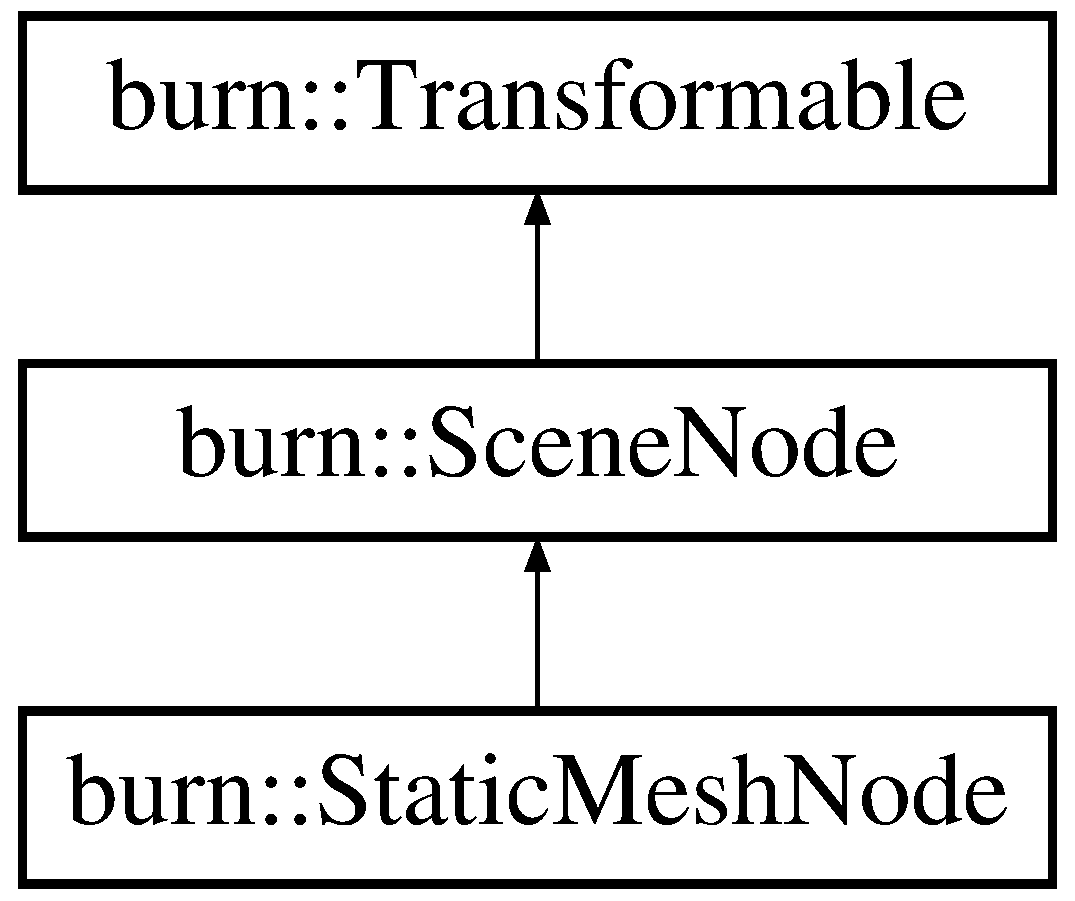
\includegraphics[height=3.000000cm]{classburn_1_1_scene_node}
\end{center}
\end{figure}
\subsection*{Public Member Functions}
\begin{DoxyCompactItemize}
\item 
\hyperlink{classburn_1_1_scene_node_a107d42062677132d1104391fd2bf2530}{Scene\-Node} ()
\begin{DoxyCompactList}\small\item\em Default Constructor. \end{DoxyCompactList}\item 
virtual \hyperlink{classburn_1_1_scene_node_aa651409167ec065930115c8b31057e35}{$\sim$\-Scene\-Node} ()
\begin{DoxyCompactList}\small\item\em Default Destructor. \end{DoxyCompactList}\item 
virtual void \hyperlink{classburn_1_1_scene_node_adcea597571e59f15421c7a9ae0bfdbc3}{draw} (\hyperlink{classburn_1_1_camera}{Camera} $\ast$camera=nullptr)=0
\begin{DoxyCompactList}\small\item\em Virtual method for rendering. \end{DoxyCompactList}\item 
const \hyperlink{classburn_1_1_material}{Material} \& \hyperlink{classburn_1_1_scene_node_a90bbe26a50c9039986bb60b52fd82a7d}{get\-Material} () const 
\begin{DoxyCompactList}\small\item\em Returns the material that the node is using. \end{DoxyCompactList}\item 
void \hyperlink{classburn_1_1_scene_node_a66ab4afa17f078a3814d4bbd88ed9ea1}{set\-Material} (const \hyperlink{classburn_1_1_material}{Material} \&material)
\begin{DoxyCompactList}\small\item\em Sets the material of the node. Influences the rendering behaviour. \end{DoxyCompactList}\end{DoxyCompactItemize}
\subsection*{Protected Attributes}
\begin{DoxyCompactItemize}
\item 
\hyperlink{classburn_1_1_material}{Material} \hyperlink{classburn_1_1_scene_node_a8474c310dafc48e860ebb5ed7ecc7f8f}{\-\_\-material}
\end{DoxyCompactItemize}


\subsection{Constructor \& Destructor Documentation}
\hypertarget{classburn_1_1_scene_node_a107d42062677132d1104391fd2bf2530}{\index{burn\-::\-Scene\-Node@{burn\-::\-Scene\-Node}!Scene\-Node@{Scene\-Node}}
\index{Scene\-Node@{Scene\-Node}!burn::SceneNode@{burn\-::\-Scene\-Node}}
\subsubsection[{Scene\-Node}]{\setlength{\rightskip}{0pt plus 5cm}burn\-::\-Scene\-Node\-::\-Scene\-Node (
\begin{DoxyParamCaption}
{}
\end{DoxyParamCaption}
)}}\label{classburn_1_1_scene_node_a107d42062677132d1104391fd2bf2530}


Default Constructor. 

\hypertarget{classburn_1_1_scene_node_aa651409167ec065930115c8b31057e35}{\index{burn\-::\-Scene\-Node@{burn\-::\-Scene\-Node}!$\sim$\-Scene\-Node@{$\sim$\-Scene\-Node}}
\index{$\sim$\-Scene\-Node@{$\sim$\-Scene\-Node}!burn::SceneNode@{burn\-::\-Scene\-Node}}
\subsubsection[{$\sim$\-Scene\-Node}]{\setlength{\rightskip}{0pt plus 5cm}burn\-::\-Scene\-Node\-::$\sim$\-Scene\-Node (
\begin{DoxyParamCaption}
{}
\end{DoxyParamCaption}
)\hspace{0.3cm}{\ttfamily [virtual]}}}\label{classburn_1_1_scene_node_aa651409167ec065930115c8b31057e35}


Default Destructor. 



\subsection{Member Function Documentation}
\hypertarget{classburn_1_1_scene_node_adcea597571e59f15421c7a9ae0bfdbc3}{\index{burn\-::\-Scene\-Node@{burn\-::\-Scene\-Node}!draw@{draw}}
\index{draw@{draw}!burn::SceneNode@{burn\-::\-Scene\-Node}}
\subsubsection[{draw}]{\setlength{\rightskip}{0pt plus 5cm}virtual void burn\-::\-Scene\-Node\-::draw (
\begin{DoxyParamCaption}
\item[{{\bf Camera} $\ast$}]{camera = {\ttfamily nullptr}}
\end{DoxyParamCaption}
)\hspace{0.3cm}{\ttfamily [pure virtual]}}}\label{classburn_1_1_scene_node_adcea597571e59f15421c7a9ae0bfdbc3}


Virtual method for rendering. 


\begin{DoxyParams}{Parameters}
{\em camera} & Pointer to \hyperlink{classburn_1_1_camera}{Camera} to draw node correctly or nullptr for default rendermode. \\
\hline
\end{DoxyParams}


Implemented in \hyperlink{classburn_1_1_static_mesh_node_a7ff88bee9757061b0393ae5324e7989b}{burn\-::\-Static\-Mesh\-Node}.

\hypertarget{classburn_1_1_scene_node_a90bbe26a50c9039986bb60b52fd82a7d}{\index{burn\-::\-Scene\-Node@{burn\-::\-Scene\-Node}!get\-Material@{get\-Material}}
\index{get\-Material@{get\-Material}!burn::SceneNode@{burn\-::\-Scene\-Node}}
\subsubsection[{get\-Material}]{\setlength{\rightskip}{0pt plus 5cm}const {\bf Material} \& burn\-::\-Scene\-Node\-::get\-Material (
\begin{DoxyParamCaption}
{}
\end{DoxyParamCaption}
) const}}\label{classburn_1_1_scene_node_a90bbe26a50c9039986bb60b52fd82a7d}


Returns the material that the node is using. 

\begin{DoxyReturn}{Returns}
The \hyperlink{classburn_1_1_material}{Material} of the node.
\end{DoxyReturn}
\begin{DoxySeeAlso}{See Also}
\hyperlink{classburn_1_1_scene_node_a66ab4afa17f078a3814d4bbd88ed9ea1}{set\-Material()} 
\end{DoxySeeAlso}
\hypertarget{classburn_1_1_scene_node_a66ab4afa17f078a3814d4bbd88ed9ea1}{\index{burn\-::\-Scene\-Node@{burn\-::\-Scene\-Node}!set\-Material@{set\-Material}}
\index{set\-Material@{set\-Material}!burn::SceneNode@{burn\-::\-Scene\-Node}}
\subsubsection[{set\-Material}]{\setlength{\rightskip}{0pt plus 5cm}void burn\-::\-Scene\-Node\-::set\-Material (
\begin{DoxyParamCaption}
\item[{const {\bf Material} \&}]{material}
\end{DoxyParamCaption}
)}}\label{classburn_1_1_scene_node_a66ab4afa17f078a3814d4bbd88ed9ea1}


Sets the material of the node. Influences the rendering behaviour. 


\begin{DoxyParams}{Parameters}
{\em material} & The \hyperlink{classburn_1_1_material}{Material} to use.\\
\hline
\end{DoxyParams}
\begin{DoxySeeAlso}{See Also}
\hyperlink{classburn_1_1_scene_node_a90bbe26a50c9039986bb60b52fd82a7d}{get\-Material()} 
\end{DoxySeeAlso}


\subsection{Member Data Documentation}
\hypertarget{classburn_1_1_scene_node_a8474c310dafc48e860ebb5ed7ecc7f8f}{\index{burn\-::\-Scene\-Node@{burn\-::\-Scene\-Node}!\-\_\-material@{\-\_\-material}}
\index{\-\_\-material@{\-\_\-material}!burn::SceneNode@{burn\-::\-Scene\-Node}}
\subsubsection[{\-\_\-material}]{\setlength{\rightskip}{0pt plus 5cm}{\bf Material} burn\-::\-Scene\-Node\-::\-\_\-material\hspace{0.3cm}{\ttfamily [protected]}}}\label{classburn_1_1_scene_node_a8474c310dafc48e860ebb5ed7ecc7f8f}


The documentation for this class was generated from the following files\-:\begin{DoxyCompactItemize}
\item 
include/\-Burngine/\-Graphics/\hyperlink{_scene_node_8h}{Scene\-Node.\-h}\item 
include/\-Burngine/\-Graphics/\hyperlink{_scene_node_8cpp}{Scene\-Node.\-cpp}\end{DoxyCompactItemize}

\hypertarget{classburn_1_1_open_gl_control_1_1_settings}{\section{burn\-:\-:Open\-Gl\-Control\-:\-:Settings Class Reference}
\label{classburn_1_1_open_gl_control_1_1_settings}\index{burn\-::\-Open\-Gl\-Control\-::\-Settings@{burn\-::\-Open\-Gl\-Control\-::\-Settings}}
}


{\ttfamily \#include $<$Open\-Gl\-Control.\-h$>$}

\subsection*{Public Member Functions}
\begin{DoxyCompactItemize}
\item 
\hyperlink{classburn_1_1_open_gl_control_1_1_settings_ac8e6ac7ffee225fbce157dd3d7ce851d}{Settings} (bool \hyperlink{classburn_1_1_open_gl_control_1_1_settings_a31424767c7990ddb3bab81a0c07112da}{is\-Blending\-Enabled}=true, const \hyperlink{classburn_1_1_open_gl_control_a2b90956aa23e041f3568234986641ba6}{Blend\-Mode} \&blend\-Mode=\hyperlink{classburn_1_1_open_gl_control_a2b90956aa23e041f3568234986641ba6ac6c8551e054abab3e0a5c554f7d4d9b6}{O\-V\-E\-R\-W\-R\-I\-T\-E}, bool \hyperlink{classburn_1_1_open_gl_control_1_1_settings_ae658f9b1d31076e2d3dee854e2a2364f}{is\-Culling\-Enabled}=true, const \hyperlink{classburn_1_1_open_gl_control_a60b866f2c1b2b210e618c39ef72f556b}{Cull\-Side} \&culled\-Side=\hyperlink{classburn_1_1_open_gl_control_a60b866f2c1b2b210e618c39ef72f556bad94f67ed661cb3c5d4d26b9429a1a28f}{I\-N\-S\-I\-D\-E}, const \hyperlink{classburn_1_1_open_gl_control_a1df746e6b8ad5c42abcfd607ef514aba}{Vertex\-Order} \&vertex\-Order=\hyperlink{classburn_1_1_open_gl_control_a1df746e6b8ad5c42abcfd607ef514abaacfe59361eeab1b7180020608a837b126}{C\-O\-U\-N\-T\-E\-R\-\_\-\-C\-L\-O\-C\-K\-W\-I\-S\-E}, bool \hyperlink{classburn_1_1_open_gl_control_1_1_settings_afc53b39d703edbc692599f9deb2a038f}{is\-Depthtest\-Enabled}=true, const \hyperlink{classburn_1_1_open_gl_control_a6435b1cdb4d2c72085a19bb77be9d845}{Depthtest\-Technique} \&technique=\hyperlink{classburn_1_1_open_gl_control_a6435b1cdb4d2c72085a19bb77be9d845a4755df5af722a2e650145662ecd8cedd}{L\-E\-S\-S}, bool \hyperlink{classburn_1_1_open_gl_control_1_1_settings_a81423f51754063178cb5c73247150e97}{is\-Depthbuffer\-Writing\-Enabled}=true, const \hyperlink{namespaceburn_a58a411b9d83c7970518a9250c1c78068}{Vector4f} \&clear\-Color=\hyperlink{namespaceburn_a58a411b9d83c7970518a9250c1c78068}{Vector4f}(0.\-1, 0.\-1, 0.\-3, 1.\-0))
\item 
void \hyperlink{classburn_1_1_open_gl_control_1_1_settings_a86141ea2923ddf7100be7d09a4f57e70}{enable\-Blending} (bool enabled=true)
\item 
bool \hyperlink{classburn_1_1_open_gl_control_1_1_settings_a31424767c7990ddb3bab81a0c07112da}{is\-Blending\-Enabled} () const 
\item 
void \hyperlink{classburn_1_1_open_gl_control_1_1_settings_a06272e79a71c5f89db3e9afbee08c87c}{set\-Blend\-Mode} (const \hyperlink{classburn_1_1_open_gl_control_a2b90956aa23e041f3568234986641ba6}{Blend\-Mode} \&blendmode)
\item 
const \hyperlink{classburn_1_1_open_gl_control_a2b90956aa23e041f3568234986641ba6}{Blend\-Mode} \& \hyperlink{classburn_1_1_open_gl_control_1_1_settings_a2caee0abe87d21d8d25d675c7bf3ce85}{get\-Blend\-Mode} () const 
\item 
void \hyperlink{classburn_1_1_open_gl_control_1_1_settings_a8a9436b332aeb7ad01dc661ff29bf120}{enable\-Culling} (bool enabled=true)
\item 
bool \hyperlink{classburn_1_1_open_gl_control_1_1_settings_ae658f9b1d31076e2d3dee854e2a2364f}{is\-Culling\-Enabled} () const 
\item 
void \hyperlink{classburn_1_1_open_gl_control_1_1_settings_abd4480405bdc2050a76319df4f9a6422}{set\-Culled\-Side} (const \hyperlink{classburn_1_1_open_gl_control_a60b866f2c1b2b210e618c39ef72f556b}{Cull\-Side} \&culled\-Side)
\item 
const \hyperlink{classburn_1_1_open_gl_control_a60b866f2c1b2b210e618c39ef72f556b}{Cull\-Side} \& \hyperlink{classburn_1_1_open_gl_control_1_1_settings_aa8b8594b7f9451a5921ab4e2c2a13660}{get\-Culled\-Side} () const 
\item 
void \hyperlink{classburn_1_1_open_gl_control_1_1_settings_a5e05f89ddf398d5d96224101cb6c6da5}{set\-Vertex\-Order} (const \hyperlink{classburn_1_1_open_gl_control_a1df746e6b8ad5c42abcfd607ef514aba}{Vertex\-Order} \&order)
\item 
const \hyperlink{classburn_1_1_open_gl_control_a1df746e6b8ad5c42abcfd607ef514aba}{Vertex\-Order} \& \hyperlink{classburn_1_1_open_gl_control_1_1_settings_a63c83ba6a41c786e81e19fe6463e7a8b}{get\-Vertex\-Order} () const 
\item 
void \hyperlink{classburn_1_1_open_gl_control_1_1_settings_ae280732e14b6e40bc75d71d084fbb606}{enable\-Depthtest} (bool enabled=true)
\item 
bool \hyperlink{classburn_1_1_open_gl_control_1_1_settings_afc53b39d703edbc692599f9deb2a038f}{is\-Depthtest\-Enabled} () const 
\item 
void \hyperlink{classburn_1_1_open_gl_control_1_1_settings_ab03c0de298099147248f541ddc1f19d7}{set\-Depthtest\-Technique} (const \hyperlink{classburn_1_1_open_gl_control_a6435b1cdb4d2c72085a19bb77be9d845}{Depthtest\-Technique} \&technique)
\item 
const \hyperlink{classburn_1_1_open_gl_control_a6435b1cdb4d2c72085a19bb77be9d845}{Depthtest\-Technique} \& \hyperlink{classburn_1_1_open_gl_control_1_1_settings_a3124638304430535f0c2246e5b28d082}{get\-Depthtest\-Technique} () const 
\item 
void \hyperlink{classburn_1_1_open_gl_control_1_1_settings_a7327bb2b002d3b5de45688853d315143}{enable\-Depthbuffer\-Writing} (bool enabled=true)
\item 
bool \hyperlink{classburn_1_1_open_gl_control_1_1_settings_a81423f51754063178cb5c73247150e97}{is\-Depthbuffer\-Writing\-Enabled} () const 
\item 
void \hyperlink{classburn_1_1_open_gl_control_1_1_settings_a20443a883ae7ef314772923438b7866a}{set\-Clear\-Color} (const \hyperlink{namespaceburn_a58a411b9d83c7970518a9250c1c78068}{Vector4f} \&color)
\item 
const \hyperlink{namespaceburn_a58a411b9d83c7970518a9250c1c78068}{Vector4f} \& \hyperlink{classburn_1_1_open_gl_control_1_1_settings_a9ac507df0d2e9d0391bbd4674242c343}{get\-Clear\-Color} () const 
\end{DoxyCompactItemize}


\subsection{Constructor \& Destructor Documentation}
\hypertarget{classburn_1_1_open_gl_control_1_1_settings_ac8e6ac7ffee225fbce157dd3d7ce851d}{\index{burn\-::\-Open\-Gl\-Control\-::\-Settings@{burn\-::\-Open\-Gl\-Control\-::\-Settings}!Settings@{Settings}}
\index{Settings@{Settings}!burn::OpenGlControl::Settings@{burn\-::\-Open\-Gl\-Control\-::\-Settings}}
\subsubsection[{Settings}]{\setlength{\rightskip}{0pt plus 5cm}burn\-::\-Open\-Gl\-Control\-::\-Settings\-::\-Settings (
\begin{DoxyParamCaption}
\item[{bool}]{is\-Blending\-Enabled = {\ttfamily true}, }
\item[{const {\bf Blend\-Mode} \&}]{blend\-Mode = {\ttfamily {\bf O\-V\-E\-R\-W\-R\-I\-T\-E}}, }
\item[{bool}]{is\-Culling\-Enabled = {\ttfamily true}, }
\item[{const {\bf Cull\-Side} \&}]{culled\-Side = {\ttfamily {\bf I\-N\-S\-I\-D\-E}}, }
\item[{const {\bf Vertex\-Order} \&}]{vertex\-Order = {\ttfamily {\bf C\-O\-U\-N\-T\-E\-R\-\_\-\-C\-L\-O\-C\-K\-W\-I\-S\-E}}, }
\item[{bool}]{is\-Depthtest\-Enabled = {\ttfamily true}, }
\item[{const {\bf Depthtest\-Technique} \&}]{technique = {\ttfamily {\bf L\-E\-S\-S}}, }
\item[{bool}]{is\-Depthbuffer\-Writing\-Enabled = {\ttfamily true}, }
\item[{const {\bf Vector4f} \&}]{clear\-Color = {\ttfamily {\bf Vector4f}(0.1,~0.1,~0.3,~1.0)}}
\end{DoxyParamCaption}
)}}\label{classburn_1_1_open_gl_control_1_1_settings_ac8e6ac7ffee225fbce157dd3d7ce851d}


\subsection{Member Function Documentation}
\hypertarget{classburn_1_1_open_gl_control_1_1_settings_a86141ea2923ddf7100be7d09a4f57e70}{\index{burn\-::\-Open\-Gl\-Control\-::\-Settings@{burn\-::\-Open\-Gl\-Control\-::\-Settings}!enable\-Blending@{enable\-Blending}}
\index{enable\-Blending@{enable\-Blending}!burn::OpenGlControl::Settings@{burn\-::\-Open\-Gl\-Control\-::\-Settings}}
\subsubsection[{enable\-Blending}]{\setlength{\rightskip}{0pt plus 5cm}void burn\-::\-Open\-Gl\-Control\-::\-Settings\-::enable\-Blending (
\begin{DoxyParamCaption}
\item[{bool}]{enabled = {\ttfamily true}}
\end{DoxyParamCaption}
)}}\label{classburn_1_1_open_gl_control_1_1_settings_a86141ea2923ddf7100be7d09a4f57e70}
\hypertarget{classburn_1_1_open_gl_control_1_1_settings_a8a9436b332aeb7ad01dc661ff29bf120}{\index{burn\-::\-Open\-Gl\-Control\-::\-Settings@{burn\-::\-Open\-Gl\-Control\-::\-Settings}!enable\-Culling@{enable\-Culling}}
\index{enable\-Culling@{enable\-Culling}!burn::OpenGlControl::Settings@{burn\-::\-Open\-Gl\-Control\-::\-Settings}}
\subsubsection[{enable\-Culling}]{\setlength{\rightskip}{0pt plus 5cm}void burn\-::\-Open\-Gl\-Control\-::\-Settings\-::enable\-Culling (
\begin{DoxyParamCaption}
\item[{bool}]{enabled = {\ttfamily true}}
\end{DoxyParamCaption}
)}}\label{classburn_1_1_open_gl_control_1_1_settings_a8a9436b332aeb7ad01dc661ff29bf120}
\hypertarget{classburn_1_1_open_gl_control_1_1_settings_a7327bb2b002d3b5de45688853d315143}{\index{burn\-::\-Open\-Gl\-Control\-::\-Settings@{burn\-::\-Open\-Gl\-Control\-::\-Settings}!enable\-Depthbuffer\-Writing@{enable\-Depthbuffer\-Writing}}
\index{enable\-Depthbuffer\-Writing@{enable\-Depthbuffer\-Writing}!burn::OpenGlControl::Settings@{burn\-::\-Open\-Gl\-Control\-::\-Settings}}
\subsubsection[{enable\-Depthbuffer\-Writing}]{\setlength{\rightskip}{0pt plus 5cm}void burn\-::\-Open\-Gl\-Control\-::\-Settings\-::enable\-Depthbuffer\-Writing (
\begin{DoxyParamCaption}
\item[{bool}]{enabled = {\ttfamily true}}
\end{DoxyParamCaption}
)}}\label{classburn_1_1_open_gl_control_1_1_settings_a7327bb2b002d3b5de45688853d315143}
\hypertarget{classburn_1_1_open_gl_control_1_1_settings_ae280732e14b6e40bc75d71d084fbb606}{\index{burn\-::\-Open\-Gl\-Control\-::\-Settings@{burn\-::\-Open\-Gl\-Control\-::\-Settings}!enable\-Depthtest@{enable\-Depthtest}}
\index{enable\-Depthtest@{enable\-Depthtest}!burn::OpenGlControl::Settings@{burn\-::\-Open\-Gl\-Control\-::\-Settings}}
\subsubsection[{enable\-Depthtest}]{\setlength{\rightskip}{0pt plus 5cm}void burn\-::\-Open\-Gl\-Control\-::\-Settings\-::enable\-Depthtest (
\begin{DoxyParamCaption}
\item[{bool}]{enabled = {\ttfamily true}}
\end{DoxyParamCaption}
)}}\label{classburn_1_1_open_gl_control_1_1_settings_ae280732e14b6e40bc75d71d084fbb606}
\hypertarget{classburn_1_1_open_gl_control_1_1_settings_a2caee0abe87d21d8d25d675c7bf3ce85}{\index{burn\-::\-Open\-Gl\-Control\-::\-Settings@{burn\-::\-Open\-Gl\-Control\-::\-Settings}!get\-Blend\-Mode@{get\-Blend\-Mode}}
\index{get\-Blend\-Mode@{get\-Blend\-Mode}!burn::OpenGlControl::Settings@{burn\-::\-Open\-Gl\-Control\-::\-Settings}}
\subsubsection[{get\-Blend\-Mode}]{\setlength{\rightskip}{0pt plus 5cm}const {\bf Blend\-Mode}\& burn\-::\-Open\-Gl\-Control\-::\-Settings\-::get\-Blend\-Mode (
\begin{DoxyParamCaption}
{}
\end{DoxyParamCaption}
) const}}\label{classburn_1_1_open_gl_control_1_1_settings_a2caee0abe87d21d8d25d675c7bf3ce85}
\hypertarget{classburn_1_1_open_gl_control_1_1_settings_a9ac507df0d2e9d0391bbd4674242c343}{\index{burn\-::\-Open\-Gl\-Control\-::\-Settings@{burn\-::\-Open\-Gl\-Control\-::\-Settings}!get\-Clear\-Color@{get\-Clear\-Color}}
\index{get\-Clear\-Color@{get\-Clear\-Color}!burn::OpenGlControl::Settings@{burn\-::\-Open\-Gl\-Control\-::\-Settings}}
\subsubsection[{get\-Clear\-Color}]{\setlength{\rightskip}{0pt plus 5cm}const {\bf Vector4f}\& burn\-::\-Open\-Gl\-Control\-::\-Settings\-::get\-Clear\-Color (
\begin{DoxyParamCaption}
{}
\end{DoxyParamCaption}
) const}}\label{classburn_1_1_open_gl_control_1_1_settings_a9ac507df0d2e9d0391bbd4674242c343}
\hypertarget{classburn_1_1_open_gl_control_1_1_settings_aa8b8594b7f9451a5921ab4e2c2a13660}{\index{burn\-::\-Open\-Gl\-Control\-::\-Settings@{burn\-::\-Open\-Gl\-Control\-::\-Settings}!get\-Culled\-Side@{get\-Culled\-Side}}
\index{get\-Culled\-Side@{get\-Culled\-Side}!burn::OpenGlControl::Settings@{burn\-::\-Open\-Gl\-Control\-::\-Settings}}
\subsubsection[{get\-Culled\-Side}]{\setlength{\rightskip}{0pt plus 5cm}const {\bf Cull\-Side}\& burn\-::\-Open\-Gl\-Control\-::\-Settings\-::get\-Culled\-Side (
\begin{DoxyParamCaption}
{}
\end{DoxyParamCaption}
) const}}\label{classburn_1_1_open_gl_control_1_1_settings_aa8b8594b7f9451a5921ab4e2c2a13660}
\hypertarget{classburn_1_1_open_gl_control_1_1_settings_a3124638304430535f0c2246e5b28d082}{\index{burn\-::\-Open\-Gl\-Control\-::\-Settings@{burn\-::\-Open\-Gl\-Control\-::\-Settings}!get\-Depthtest\-Technique@{get\-Depthtest\-Technique}}
\index{get\-Depthtest\-Technique@{get\-Depthtest\-Technique}!burn::OpenGlControl::Settings@{burn\-::\-Open\-Gl\-Control\-::\-Settings}}
\subsubsection[{get\-Depthtest\-Technique}]{\setlength{\rightskip}{0pt plus 5cm}const {\bf Depthtest\-Technique}\& burn\-::\-Open\-Gl\-Control\-::\-Settings\-::get\-Depthtest\-Technique (
\begin{DoxyParamCaption}
{}
\end{DoxyParamCaption}
) const}}\label{classburn_1_1_open_gl_control_1_1_settings_a3124638304430535f0c2246e5b28d082}
\hypertarget{classburn_1_1_open_gl_control_1_1_settings_a63c83ba6a41c786e81e19fe6463e7a8b}{\index{burn\-::\-Open\-Gl\-Control\-::\-Settings@{burn\-::\-Open\-Gl\-Control\-::\-Settings}!get\-Vertex\-Order@{get\-Vertex\-Order}}
\index{get\-Vertex\-Order@{get\-Vertex\-Order}!burn::OpenGlControl::Settings@{burn\-::\-Open\-Gl\-Control\-::\-Settings}}
\subsubsection[{get\-Vertex\-Order}]{\setlength{\rightskip}{0pt plus 5cm}const {\bf Vertex\-Order}\& burn\-::\-Open\-Gl\-Control\-::\-Settings\-::get\-Vertex\-Order (
\begin{DoxyParamCaption}
{}
\end{DoxyParamCaption}
) const}}\label{classburn_1_1_open_gl_control_1_1_settings_a63c83ba6a41c786e81e19fe6463e7a8b}
\hypertarget{classburn_1_1_open_gl_control_1_1_settings_a31424767c7990ddb3bab81a0c07112da}{\index{burn\-::\-Open\-Gl\-Control\-::\-Settings@{burn\-::\-Open\-Gl\-Control\-::\-Settings}!is\-Blending\-Enabled@{is\-Blending\-Enabled}}
\index{is\-Blending\-Enabled@{is\-Blending\-Enabled}!burn::OpenGlControl::Settings@{burn\-::\-Open\-Gl\-Control\-::\-Settings}}
\subsubsection[{is\-Blending\-Enabled}]{\setlength{\rightskip}{0pt plus 5cm}bool burn\-::\-Open\-Gl\-Control\-::\-Settings\-::is\-Blending\-Enabled (
\begin{DoxyParamCaption}
{}
\end{DoxyParamCaption}
) const}}\label{classburn_1_1_open_gl_control_1_1_settings_a31424767c7990ddb3bab81a0c07112da}
\hypertarget{classburn_1_1_open_gl_control_1_1_settings_ae658f9b1d31076e2d3dee854e2a2364f}{\index{burn\-::\-Open\-Gl\-Control\-::\-Settings@{burn\-::\-Open\-Gl\-Control\-::\-Settings}!is\-Culling\-Enabled@{is\-Culling\-Enabled}}
\index{is\-Culling\-Enabled@{is\-Culling\-Enabled}!burn::OpenGlControl::Settings@{burn\-::\-Open\-Gl\-Control\-::\-Settings}}
\subsubsection[{is\-Culling\-Enabled}]{\setlength{\rightskip}{0pt plus 5cm}bool burn\-::\-Open\-Gl\-Control\-::\-Settings\-::is\-Culling\-Enabled (
\begin{DoxyParamCaption}
{}
\end{DoxyParamCaption}
) const}}\label{classburn_1_1_open_gl_control_1_1_settings_ae658f9b1d31076e2d3dee854e2a2364f}
\hypertarget{classburn_1_1_open_gl_control_1_1_settings_a81423f51754063178cb5c73247150e97}{\index{burn\-::\-Open\-Gl\-Control\-::\-Settings@{burn\-::\-Open\-Gl\-Control\-::\-Settings}!is\-Depthbuffer\-Writing\-Enabled@{is\-Depthbuffer\-Writing\-Enabled}}
\index{is\-Depthbuffer\-Writing\-Enabled@{is\-Depthbuffer\-Writing\-Enabled}!burn::OpenGlControl::Settings@{burn\-::\-Open\-Gl\-Control\-::\-Settings}}
\subsubsection[{is\-Depthbuffer\-Writing\-Enabled}]{\setlength{\rightskip}{0pt plus 5cm}bool burn\-::\-Open\-Gl\-Control\-::\-Settings\-::is\-Depthbuffer\-Writing\-Enabled (
\begin{DoxyParamCaption}
{}
\end{DoxyParamCaption}
) const}}\label{classburn_1_1_open_gl_control_1_1_settings_a81423f51754063178cb5c73247150e97}
\hypertarget{classburn_1_1_open_gl_control_1_1_settings_afc53b39d703edbc692599f9deb2a038f}{\index{burn\-::\-Open\-Gl\-Control\-::\-Settings@{burn\-::\-Open\-Gl\-Control\-::\-Settings}!is\-Depthtest\-Enabled@{is\-Depthtest\-Enabled}}
\index{is\-Depthtest\-Enabled@{is\-Depthtest\-Enabled}!burn::OpenGlControl::Settings@{burn\-::\-Open\-Gl\-Control\-::\-Settings}}
\subsubsection[{is\-Depthtest\-Enabled}]{\setlength{\rightskip}{0pt plus 5cm}bool burn\-::\-Open\-Gl\-Control\-::\-Settings\-::is\-Depthtest\-Enabled (
\begin{DoxyParamCaption}
{}
\end{DoxyParamCaption}
) const}}\label{classburn_1_1_open_gl_control_1_1_settings_afc53b39d703edbc692599f9deb2a038f}
\hypertarget{classburn_1_1_open_gl_control_1_1_settings_a06272e79a71c5f89db3e9afbee08c87c}{\index{burn\-::\-Open\-Gl\-Control\-::\-Settings@{burn\-::\-Open\-Gl\-Control\-::\-Settings}!set\-Blend\-Mode@{set\-Blend\-Mode}}
\index{set\-Blend\-Mode@{set\-Blend\-Mode}!burn::OpenGlControl::Settings@{burn\-::\-Open\-Gl\-Control\-::\-Settings}}
\subsubsection[{set\-Blend\-Mode}]{\setlength{\rightskip}{0pt plus 5cm}void burn\-::\-Open\-Gl\-Control\-::\-Settings\-::set\-Blend\-Mode (
\begin{DoxyParamCaption}
\item[{const {\bf Blend\-Mode} \&}]{blendmode}
\end{DoxyParamCaption}
)}}\label{classburn_1_1_open_gl_control_1_1_settings_a06272e79a71c5f89db3e9afbee08c87c}
\hypertarget{classburn_1_1_open_gl_control_1_1_settings_a20443a883ae7ef314772923438b7866a}{\index{burn\-::\-Open\-Gl\-Control\-::\-Settings@{burn\-::\-Open\-Gl\-Control\-::\-Settings}!set\-Clear\-Color@{set\-Clear\-Color}}
\index{set\-Clear\-Color@{set\-Clear\-Color}!burn::OpenGlControl::Settings@{burn\-::\-Open\-Gl\-Control\-::\-Settings}}
\subsubsection[{set\-Clear\-Color}]{\setlength{\rightskip}{0pt plus 5cm}void burn\-::\-Open\-Gl\-Control\-::\-Settings\-::set\-Clear\-Color (
\begin{DoxyParamCaption}
\item[{const {\bf Vector4f} \&}]{color}
\end{DoxyParamCaption}
)}}\label{classburn_1_1_open_gl_control_1_1_settings_a20443a883ae7ef314772923438b7866a}
\hypertarget{classburn_1_1_open_gl_control_1_1_settings_abd4480405bdc2050a76319df4f9a6422}{\index{burn\-::\-Open\-Gl\-Control\-::\-Settings@{burn\-::\-Open\-Gl\-Control\-::\-Settings}!set\-Culled\-Side@{set\-Culled\-Side}}
\index{set\-Culled\-Side@{set\-Culled\-Side}!burn::OpenGlControl::Settings@{burn\-::\-Open\-Gl\-Control\-::\-Settings}}
\subsubsection[{set\-Culled\-Side}]{\setlength{\rightskip}{0pt plus 5cm}void burn\-::\-Open\-Gl\-Control\-::\-Settings\-::set\-Culled\-Side (
\begin{DoxyParamCaption}
\item[{const {\bf Cull\-Side} \&}]{culled\-Side}
\end{DoxyParamCaption}
)}}\label{classburn_1_1_open_gl_control_1_1_settings_abd4480405bdc2050a76319df4f9a6422}
\hypertarget{classburn_1_1_open_gl_control_1_1_settings_ab03c0de298099147248f541ddc1f19d7}{\index{burn\-::\-Open\-Gl\-Control\-::\-Settings@{burn\-::\-Open\-Gl\-Control\-::\-Settings}!set\-Depthtest\-Technique@{set\-Depthtest\-Technique}}
\index{set\-Depthtest\-Technique@{set\-Depthtest\-Technique}!burn::OpenGlControl::Settings@{burn\-::\-Open\-Gl\-Control\-::\-Settings}}
\subsubsection[{set\-Depthtest\-Technique}]{\setlength{\rightskip}{0pt plus 5cm}void burn\-::\-Open\-Gl\-Control\-::\-Settings\-::set\-Depthtest\-Technique (
\begin{DoxyParamCaption}
\item[{const {\bf Depthtest\-Technique} \&}]{technique}
\end{DoxyParamCaption}
)}}\label{classburn_1_1_open_gl_control_1_1_settings_ab03c0de298099147248f541ddc1f19d7}
\hypertarget{classburn_1_1_open_gl_control_1_1_settings_a5e05f89ddf398d5d96224101cb6c6da5}{\index{burn\-::\-Open\-Gl\-Control\-::\-Settings@{burn\-::\-Open\-Gl\-Control\-::\-Settings}!set\-Vertex\-Order@{set\-Vertex\-Order}}
\index{set\-Vertex\-Order@{set\-Vertex\-Order}!burn::OpenGlControl::Settings@{burn\-::\-Open\-Gl\-Control\-::\-Settings}}
\subsubsection[{set\-Vertex\-Order}]{\setlength{\rightskip}{0pt plus 5cm}void burn\-::\-Open\-Gl\-Control\-::\-Settings\-::set\-Vertex\-Order (
\begin{DoxyParamCaption}
\item[{const {\bf Vertex\-Order} \&}]{order}
\end{DoxyParamCaption}
)}}\label{classburn_1_1_open_gl_control_1_1_settings_a5e05f89ddf398d5d96224101cb6c6da5}


The documentation for this class was generated from the following file\-:\begin{DoxyCompactItemize}
\item 
include/\-Burngine/\-Graphics/\-General/\hyperlink{_open_gl_control_8h}{Open\-Gl\-Control.\-h}\end{DoxyCompactItemize}

\hypertarget{classburn_1_1_shader}{\section{burn\-:\-:Shader Class Reference}
\label{classburn_1_1_shader}\index{burn\-::\-Shader@{burn\-::\-Shader}}
}


{\ttfamily \#include $<$Shader.\-h$>$}

\subsection*{Public Member Functions}
\begin{DoxyCompactItemize}
\item 
\hyperlink{classburn_1_1_shader_a9795869452f44ff05a2a4b1f278bc990}{Shader} ()
\begin{DoxyCompactList}\small\item\em Default constructor. Default values\-: \end{DoxyCompactList}\item 
\hyperlink{classburn_1_1_shader_a4f67c0a15b6cf9146869cfbcdbdfb541}{$\sim$\-Shader} ()
\begin{DoxyCompactList}\small\item\em Default destructor. Deletes shaderprogram from Open\-G\-L if needed. \end{DoxyCompactList}\item 
bool \hyperlink{classburn_1_1_shader_ae2975b4b68d38d8aa3d045df082e7c2a}{load\-From\-String} (const std\-::string \&vertex\-Shader, const std\-::string \&fragment\-Shader)
\begin{DoxyCompactList}\small\item\em Loads and creates shaderprograms by passing in a vertex-\/ and fragmentshader. \end{DoxyCompactList}\item 
void \hyperlink{classburn_1_1_shader_a8f476e17b38b96d84ea57c31d7aab78d}{activate} () const 
\begin{DoxyCompactList}\small\item\em Activates the shader. It will be used for rendering until no other \hyperlink{classburn_1_1_shader}{Shader} had been called or this one had been destroyed. \end{DoxyCompactList}\item 
G\-Luint \hyperlink{classburn_1_1_shader_ae96b86c6da489d759bec9be7664040dc}{get\-Uniform\-Location} (const std\-::string \&uniform\-Name) const 
\begin{DoxyCompactList}\small\item\em Returns the position of a uniform inside the shaderprogram. This is useful to pass matrices for example. Internal usage mostly. \end{DoxyCompactList}\end{DoxyCompactItemize}


\subsection{Constructor \& Destructor Documentation}
\hypertarget{classburn_1_1_shader_a9795869452f44ff05a2a4b1f278bc990}{\index{burn\-::\-Shader@{burn\-::\-Shader}!Shader@{Shader}}
\index{Shader@{Shader}!burn::Shader@{burn\-::\-Shader}}
\subsubsection[{Shader}]{\setlength{\rightskip}{0pt plus 5cm}burn\-::\-Shader\-::\-Shader (
\begin{DoxyParamCaption}
{}
\end{DoxyParamCaption}
)}}\label{classburn_1_1_shader_a9795869452f44ff05a2a4b1f278bc990}


Default constructor. Default values\-: 


\begin{DoxyItemize}
\item I\-D\-: 0 (invalid I\-D) 
\end{DoxyItemize}\hypertarget{classburn_1_1_shader_a4f67c0a15b6cf9146869cfbcdbdfb541}{\index{burn\-::\-Shader@{burn\-::\-Shader}!$\sim$\-Shader@{$\sim$\-Shader}}
\index{$\sim$\-Shader@{$\sim$\-Shader}!burn::Shader@{burn\-::\-Shader}}
\subsubsection[{$\sim$\-Shader}]{\setlength{\rightskip}{0pt plus 5cm}burn\-::\-Shader\-::$\sim$\-Shader (
\begin{DoxyParamCaption}
{}
\end{DoxyParamCaption}
)}}\label{classburn_1_1_shader_a4f67c0a15b6cf9146869cfbcdbdfb541}


Default destructor. Deletes shaderprogram from Open\-G\-L if needed. 



\subsection{Member Function Documentation}
\hypertarget{classburn_1_1_shader_a8f476e17b38b96d84ea57c31d7aab78d}{\index{burn\-::\-Shader@{burn\-::\-Shader}!activate@{activate}}
\index{activate@{activate}!burn::Shader@{burn\-::\-Shader}}
\subsubsection[{activate}]{\setlength{\rightskip}{0pt plus 5cm}void burn\-::\-Shader\-::activate (
\begin{DoxyParamCaption}
{}
\end{DoxyParamCaption}
) const}}\label{classburn_1_1_shader_a8f476e17b38b96d84ea57c31d7aab78d}


Activates the shader. It will be used for rendering until no other \hyperlink{classburn_1_1_shader}{Shader} had been called or this one had been destroyed. 

\begin{DoxyNote}{Note}
If no \hyperlink{classburn_1_1_shader}{Shader} was created by e.\-g. calling \hyperlink{classburn_1_1_shader_ae2975b4b68d38d8aa3d045df082e7c2a}{load\-From\-String()}, this call will disable shaders at all.
\end{DoxyNote}
\begin{DoxySeeAlso}{See Also}
\hyperlink{classburn_1_1_shader_ae2975b4b68d38d8aa3d045df082e7c2a}{load\-From\-String()} 
\end{DoxySeeAlso}
\hypertarget{classburn_1_1_shader_ae96b86c6da489d759bec9be7664040dc}{\index{burn\-::\-Shader@{burn\-::\-Shader}!get\-Uniform\-Location@{get\-Uniform\-Location}}
\index{get\-Uniform\-Location@{get\-Uniform\-Location}!burn::Shader@{burn\-::\-Shader}}
\subsubsection[{get\-Uniform\-Location}]{\setlength{\rightskip}{0pt plus 5cm}G\-Luint burn\-::\-Shader\-::get\-Uniform\-Location (
\begin{DoxyParamCaption}
\item[{const std\-::string \&}]{uniform\-Name}
\end{DoxyParamCaption}
) const}}\label{classburn_1_1_shader_ae96b86c6da489d759bec9be7664040dc}


Returns the position of a uniform inside the shaderprogram. This is useful to pass matrices for example. Internal usage mostly. 


\begin{DoxyParams}{Parameters}
{\em uniform\-Name} & The name of the uniform.\\
\hline
\end{DoxyParams}
\begin{DoxyReturn}{Returns}
Returns a value $>$= 0 on success or -\/1 when the uniform could not be found. 
\end{DoxyReturn}
\hypertarget{classburn_1_1_shader_ae2975b4b68d38d8aa3d045df082e7c2a}{\index{burn\-::\-Shader@{burn\-::\-Shader}!load\-From\-String@{load\-From\-String}}
\index{load\-From\-String@{load\-From\-String}!burn::Shader@{burn\-::\-Shader}}
\subsubsection[{load\-From\-String}]{\setlength{\rightskip}{0pt plus 5cm}bool burn\-::\-Shader\-::load\-From\-String (
\begin{DoxyParamCaption}
\item[{const std\-::string \&}]{vertex\-Shader, }
\item[{const std\-::string \&}]{fragment\-Shader}
\end{DoxyParamCaption}
)}}\label{classburn_1_1_shader_ae2975b4b68d38d8aa3d045df082e7c2a}


Loads and creates shaderprograms by passing in a vertex-\/ and fragmentshader. 


\begin{DoxyParams}{Parameters}
{\em vertex\-Shader} & The vertexshader. \\
\hline
{\em fragment\-Shader} & The fragmentshader.\\
\hline
\end{DoxyParams}
\begin{DoxyReturn}{Returns}
Returns true when shader was created successfully.
\end{DoxyReturn}
\begin{DoxySeeAlso}{See Also}
\hyperlink{classburn_1_1_shader_a8f476e17b38b96d84ea57c31d7aab78d}{activate()} 
\end{DoxySeeAlso}


The documentation for this class was generated from the following files\-:\begin{DoxyCompactItemize}
\item 
include/\-Burngine/\-Graphics/\hyperlink{_shader_8h}{Shader.\-h}\item 
include/\-Burngine/\-Graphics/\hyperlink{_shader_8cpp}{Shader.\-cpp}\end{DoxyCompactItemize}

\hypertarget{classburn_1_1_shadow_cube_map}{\section{burn\-:\-:Shadow\-Cube\-Map Class Reference}
\label{classburn_1_1_shadow_cube_map}\index{burn\-::\-Shadow\-Cube\-Map@{burn\-::\-Shadow\-Cube\-Map}}
}


{\ttfamily \#include $<$Shadow\-Cube\-Map.\-h$>$}

Inheritance diagram for burn\-:\-:Shadow\-Cube\-Map\-:\begin{figure}[H]
\begin{center}
\leavevmode
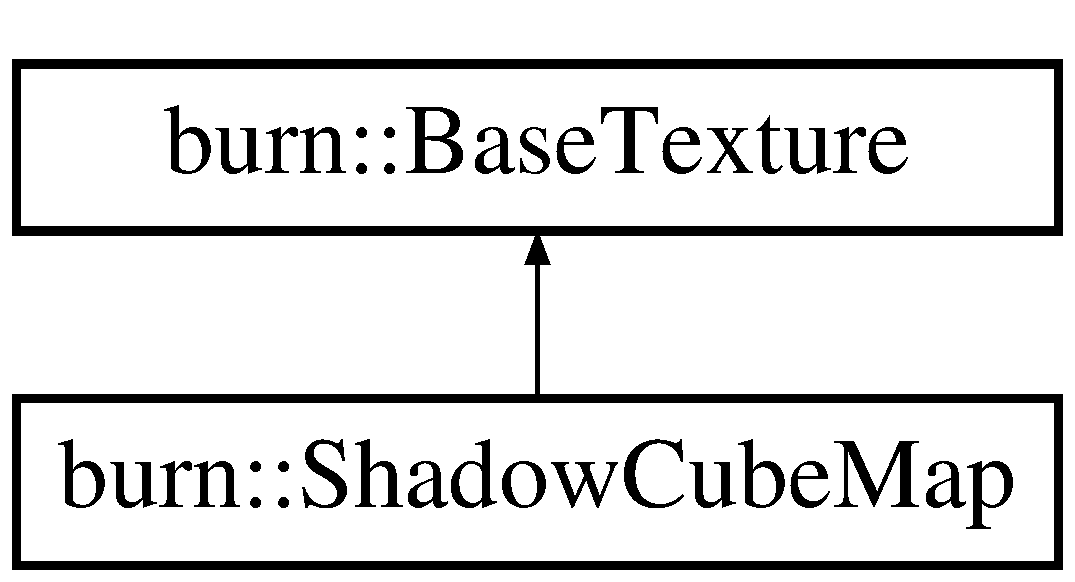
\includegraphics[height=2.000000cm]{classburn_1_1_shadow_cube_map}
\end{center}
\end{figure}
\subsection*{Public Types}
\begin{DoxyCompactItemize}
\item 
enum \hyperlink{classburn_1_1_shadow_cube_map_a199f4c817b2cadb4f3b93c270c4f209e}{Resolution} \{ \\*
\hyperlink{classburn_1_1_shadow_cube_map_a199f4c817b2cadb4f3b93c270c4f209ea879262ad62b035c8d4b20c0eaac7896c}{V\-E\-R\-Y\-\_\-\-L\-O\-W} = 128, 
\hyperlink{classburn_1_1_shadow_cube_map_a199f4c817b2cadb4f3b93c270c4f209ea04beb22bfc324a3458294be49d313c9c}{L\-O\-W} = 256, 
\hyperlink{classburn_1_1_shadow_cube_map_a199f4c817b2cadb4f3b93c270c4f209ea880badf96feef25667391e15b62516e0}{M\-E\-D\-I\-U\-M} = 512, 
\hyperlink{classburn_1_1_shadow_cube_map_a199f4c817b2cadb4f3b93c270c4f209eadec66121357f641252b33af54af06eab}{H\-I\-G\-H} = 1024, 
\\*
\hyperlink{classburn_1_1_shadow_cube_map_a199f4c817b2cadb4f3b93c270c4f209eab857a7ffa30e1ef01b8eece6667473a5}{V\-E\-R\-Y\-\_\-\-H\-I\-G\-H} = 2048
 \}
\end{DoxyCompactItemize}
\subsection*{Public Member Functions}
\begin{DoxyCompactItemize}
\item 
\hyperlink{classburn_1_1_shadow_cube_map_a599b548269fabfd0ee97e1d5ce9f38a9}{Shadow\-Cube\-Map} ()
\item 
\hyperlink{classburn_1_1_shadow_cube_map_a3d9ddc7204cdc28972e34607c323858a}{Shadow\-Cube\-Map} (const \hyperlink{classburn_1_1_shadow_cube_map}{Shadow\-Cube\-Map} \&other)=delete
\item 
\hyperlink{classburn_1_1_shadow_cube_map}{Shadow\-Cube\-Map} \& \hyperlink{classburn_1_1_shadow_cube_map_ad6121442fd4c9e91ec80b1c1f49241ef}{operator=} (const \hyperlink{classburn_1_1_shadow_cube_map}{Shadow\-Cube\-Map} \&other)=delete
\item 
\hyperlink{classburn_1_1_shadow_cube_map_ae42dcafba18ff6617621fec719d9bd7f}{$\sim$\-Shadow\-Cube\-Map} ()
\item 
bool \hyperlink{classburn_1_1_shadow_cube_map_adfed32062083f0a6ee604afd737141ed}{create} (const \hyperlink{classburn_1_1_shadow_cube_map_a199f4c817b2cadb4f3b93c270c4f209e}{Resolution} \&resolution=\hyperlink{classburn_1_1_shadow_cube_map_a199f4c817b2cadb4f3b93c270c4f209eadec66121357f641252b33af54af06eab}{H\-I\-G\-H})
\item 
void \hyperlink{classburn_1_1_shadow_cube_map_a20303d8a205cf66cb5b9e979fb868c88}{clear} ()
\item 
void \hyperlink{classburn_1_1_shadow_cube_map_a410af6be57e69747cbdc7c4fbe05873b}{bind\-As\-Rendertarget} (const int \&face) const 
\item 
bool \hyperlink{classburn_1_1_shadow_cube_map_a284df2f4e4f5440e5290208aa59a0c68}{is\-Created} () const 
\item 
const \hyperlink{classburn_1_1_shadow_cube_map_a199f4c817b2cadb4f3b93c270c4f209e}{Resolution} \& \hyperlink{classburn_1_1_shadow_cube_map_abe6912373648fbde0ee90d894ec92db1}{get\-Resolution} () const 
\end{DoxyCompactItemize}
\subsection*{Additional Inherited Members}


\subsection{Member Enumeration Documentation}
\hypertarget{classburn_1_1_shadow_cube_map_a199f4c817b2cadb4f3b93c270c4f209e}{\index{burn\-::\-Shadow\-Cube\-Map@{burn\-::\-Shadow\-Cube\-Map}!Resolution@{Resolution}}
\index{Resolution@{Resolution}!burn::ShadowCubeMap@{burn\-::\-Shadow\-Cube\-Map}}
\subsubsection[{Resolution}]{\setlength{\rightskip}{0pt plus 5cm}enum {\bf burn\-::\-Shadow\-Cube\-Map\-::\-Resolution}}}\label{classburn_1_1_shadow_cube_map_a199f4c817b2cadb4f3b93c270c4f209e}
\begin{Desc}
\item[Enumerator]\par
\begin{description}
\index{V\-E\-R\-Y\-\_\-\-L\-O\-W@{V\-E\-R\-Y\-\_\-\-L\-O\-W}!burn\-::\-Shadow\-Cube\-Map@{burn\-::\-Shadow\-Cube\-Map}}\index{burn\-::\-Shadow\-Cube\-Map@{burn\-::\-Shadow\-Cube\-Map}!V\-E\-R\-Y\-\_\-\-L\-O\-W@{V\-E\-R\-Y\-\_\-\-L\-O\-W}}\item[{\em 
\hypertarget{classburn_1_1_shadow_cube_map_a199f4c817b2cadb4f3b93c270c4f209ea879262ad62b035c8d4b20c0eaac7896c}{V\-E\-R\-Y\-\_\-\-L\-O\-W}\label{classburn_1_1_shadow_cube_map_a199f4c817b2cadb4f3b93c270c4f209ea879262ad62b035c8d4b20c0eaac7896c}
}]128x128 \index{L\-O\-W@{L\-O\-W}!burn\-::\-Shadow\-Cube\-Map@{burn\-::\-Shadow\-Cube\-Map}}\index{burn\-::\-Shadow\-Cube\-Map@{burn\-::\-Shadow\-Cube\-Map}!L\-O\-W@{L\-O\-W}}\item[{\em 
\hypertarget{classburn_1_1_shadow_cube_map_a199f4c817b2cadb4f3b93c270c4f209ea04beb22bfc324a3458294be49d313c9c}{L\-O\-W}\label{classburn_1_1_shadow_cube_map_a199f4c817b2cadb4f3b93c270c4f209ea04beb22bfc324a3458294be49d313c9c}
}]256x256 \index{M\-E\-D\-I\-U\-M@{M\-E\-D\-I\-U\-M}!burn\-::\-Shadow\-Cube\-Map@{burn\-::\-Shadow\-Cube\-Map}}\index{burn\-::\-Shadow\-Cube\-Map@{burn\-::\-Shadow\-Cube\-Map}!M\-E\-D\-I\-U\-M@{M\-E\-D\-I\-U\-M}}\item[{\em 
\hypertarget{classburn_1_1_shadow_cube_map_a199f4c817b2cadb4f3b93c270c4f209ea880badf96feef25667391e15b62516e0}{M\-E\-D\-I\-U\-M}\label{classburn_1_1_shadow_cube_map_a199f4c817b2cadb4f3b93c270c4f209ea880badf96feef25667391e15b62516e0}
}]512x512 \index{H\-I\-G\-H@{H\-I\-G\-H}!burn\-::\-Shadow\-Cube\-Map@{burn\-::\-Shadow\-Cube\-Map}}\index{burn\-::\-Shadow\-Cube\-Map@{burn\-::\-Shadow\-Cube\-Map}!H\-I\-G\-H@{H\-I\-G\-H}}\item[{\em 
\hypertarget{classburn_1_1_shadow_cube_map_a199f4c817b2cadb4f3b93c270c4f209eadec66121357f641252b33af54af06eab}{H\-I\-G\-H}\label{classburn_1_1_shadow_cube_map_a199f4c817b2cadb4f3b93c270c4f209eadec66121357f641252b33af54af06eab}
}]1024x1024 \index{V\-E\-R\-Y\-\_\-\-H\-I\-G\-H@{V\-E\-R\-Y\-\_\-\-H\-I\-G\-H}!burn\-::\-Shadow\-Cube\-Map@{burn\-::\-Shadow\-Cube\-Map}}\index{burn\-::\-Shadow\-Cube\-Map@{burn\-::\-Shadow\-Cube\-Map}!V\-E\-R\-Y\-\_\-\-H\-I\-G\-H@{V\-E\-R\-Y\-\_\-\-H\-I\-G\-H}}\item[{\em 
\hypertarget{classburn_1_1_shadow_cube_map_a199f4c817b2cadb4f3b93c270c4f209eab857a7ffa30e1ef01b8eece6667473a5}{V\-E\-R\-Y\-\_\-\-H\-I\-G\-H}\label{classburn_1_1_shadow_cube_map_a199f4c817b2cadb4f3b93c270c4f209eab857a7ffa30e1ef01b8eece6667473a5}
}]2048x2048 \end{description}
\end{Desc}


\subsection{Constructor \& Destructor Documentation}
\hypertarget{classburn_1_1_shadow_cube_map_a599b548269fabfd0ee97e1d5ce9f38a9}{\index{burn\-::\-Shadow\-Cube\-Map@{burn\-::\-Shadow\-Cube\-Map}!Shadow\-Cube\-Map@{Shadow\-Cube\-Map}}
\index{Shadow\-Cube\-Map@{Shadow\-Cube\-Map}!burn::ShadowCubeMap@{burn\-::\-Shadow\-Cube\-Map}}
\subsubsection[{Shadow\-Cube\-Map}]{\setlength{\rightskip}{0pt plus 5cm}burn\-::\-Shadow\-Cube\-Map\-::\-Shadow\-Cube\-Map (
\begin{DoxyParamCaption}
{}
\end{DoxyParamCaption}
)}}\label{classburn_1_1_shadow_cube_map_a599b548269fabfd0ee97e1d5ce9f38a9}
\hypertarget{classburn_1_1_shadow_cube_map_a3d9ddc7204cdc28972e34607c323858a}{\index{burn\-::\-Shadow\-Cube\-Map@{burn\-::\-Shadow\-Cube\-Map}!Shadow\-Cube\-Map@{Shadow\-Cube\-Map}}
\index{Shadow\-Cube\-Map@{Shadow\-Cube\-Map}!burn::ShadowCubeMap@{burn\-::\-Shadow\-Cube\-Map}}
\subsubsection[{Shadow\-Cube\-Map}]{\setlength{\rightskip}{0pt plus 5cm}burn\-::\-Shadow\-Cube\-Map\-::\-Shadow\-Cube\-Map (
\begin{DoxyParamCaption}
\item[{const {\bf Shadow\-Cube\-Map} \&}]{other}
\end{DoxyParamCaption}
)\hspace{0.3cm}{\ttfamily [delete]}}}\label{classburn_1_1_shadow_cube_map_a3d9ddc7204cdc28972e34607c323858a}
\hypertarget{classburn_1_1_shadow_cube_map_ae42dcafba18ff6617621fec719d9bd7f}{\index{burn\-::\-Shadow\-Cube\-Map@{burn\-::\-Shadow\-Cube\-Map}!$\sim$\-Shadow\-Cube\-Map@{$\sim$\-Shadow\-Cube\-Map}}
\index{$\sim$\-Shadow\-Cube\-Map@{$\sim$\-Shadow\-Cube\-Map}!burn::ShadowCubeMap@{burn\-::\-Shadow\-Cube\-Map}}
\subsubsection[{$\sim$\-Shadow\-Cube\-Map}]{\setlength{\rightskip}{0pt plus 5cm}burn\-::\-Shadow\-Cube\-Map\-::$\sim$\-Shadow\-Cube\-Map (
\begin{DoxyParamCaption}
{}
\end{DoxyParamCaption}
)}}\label{classburn_1_1_shadow_cube_map_ae42dcafba18ff6617621fec719d9bd7f}


\subsection{Member Function Documentation}
\hypertarget{classburn_1_1_shadow_cube_map_a410af6be57e69747cbdc7c4fbe05873b}{\index{burn\-::\-Shadow\-Cube\-Map@{burn\-::\-Shadow\-Cube\-Map}!bind\-As\-Rendertarget@{bind\-As\-Rendertarget}}
\index{bind\-As\-Rendertarget@{bind\-As\-Rendertarget}!burn::ShadowCubeMap@{burn\-::\-Shadow\-Cube\-Map}}
\subsubsection[{bind\-As\-Rendertarget}]{\setlength{\rightskip}{0pt plus 5cm}void burn\-::\-Shadow\-Cube\-Map\-::bind\-As\-Rendertarget (
\begin{DoxyParamCaption}
\item[{const int \&}]{face}
\end{DoxyParamCaption}
) const}}\label{classburn_1_1_shadow_cube_map_a410af6be57e69747cbdc7c4fbe05873b}
\hypertarget{classburn_1_1_shadow_cube_map_a20303d8a205cf66cb5b9e979fb868c88}{\index{burn\-::\-Shadow\-Cube\-Map@{burn\-::\-Shadow\-Cube\-Map}!clear@{clear}}
\index{clear@{clear}!burn::ShadowCubeMap@{burn\-::\-Shadow\-Cube\-Map}}
\subsubsection[{clear}]{\setlength{\rightskip}{0pt plus 5cm}void burn\-::\-Shadow\-Cube\-Map\-::clear (
\begin{DoxyParamCaption}
{}
\end{DoxyParamCaption}
)}}\label{classburn_1_1_shadow_cube_map_a20303d8a205cf66cb5b9e979fb868c88}
\hypertarget{classburn_1_1_shadow_cube_map_adfed32062083f0a6ee604afd737141ed}{\index{burn\-::\-Shadow\-Cube\-Map@{burn\-::\-Shadow\-Cube\-Map}!create@{create}}
\index{create@{create}!burn::ShadowCubeMap@{burn\-::\-Shadow\-Cube\-Map}}
\subsubsection[{create}]{\setlength{\rightskip}{0pt plus 5cm}bool burn\-::\-Shadow\-Cube\-Map\-::create (
\begin{DoxyParamCaption}
\item[{const {\bf Resolution} \&}]{resolution = {\ttfamily {\bf H\-I\-G\-H}}}
\end{DoxyParamCaption}
)}}\label{classburn_1_1_shadow_cube_map_adfed32062083f0a6ee604afd737141ed}
\hypertarget{classburn_1_1_shadow_cube_map_abe6912373648fbde0ee90d894ec92db1}{\index{burn\-::\-Shadow\-Cube\-Map@{burn\-::\-Shadow\-Cube\-Map}!get\-Resolution@{get\-Resolution}}
\index{get\-Resolution@{get\-Resolution}!burn::ShadowCubeMap@{burn\-::\-Shadow\-Cube\-Map}}
\subsubsection[{get\-Resolution}]{\setlength{\rightskip}{0pt plus 5cm}const {\bf Resolution}\& burn\-::\-Shadow\-Cube\-Map\-::get\-Resolution (
\begin{DoxyParamCaption}
{}
\end{DoxyParamCaption}
) const}}\label{classburn_1_1_shadow_cube_map_abe6912373648fbde0ee90d894ec92db1}
\hypertarget{classburn_1_1_shadow_cube_map_a284df2f4e4f5440e5290208aa59a0c68}{\index{burn\-::\-Shadow\-Cube\-Map@{burn\-::\-Shadow\-Cube\-Map}!is\-Created@{is\-Created}}
\index{is\-Created@{is\-Created}!burn::ShadowCubeMap@{burn\-::\-Shadow\-Cube\-Map}}
\subsubsection[{is\-Created}]{\setlength{\rightskip}{0pt plus 5cm}bool burn\-::\-Shadow\-Cube\-Map\-::is\-Created (
\begin{DoxyParamCaption}
{}
\end{DoxyParamCaption}
) const}}\label{classburn_1_1_shadow_cube_map_a284df2f4e4f5440e5290208aa59a0c68}
\hypertarget{classburn_1_1_shadow_cube_map_ad6121442fd4c9e91ec80b1c1f49241ef}{\index{burn\-::\-Shadow\-Cube\-Map@{burn\-::\-Shadow\-Cube\-Map}!operator=@{operator=}}
\index{operator=@{operator=}!burn::ShadowCubeMap@{burn\-::\-Shadow\-Cube\-Map}}
\subsubsection[{operator=}]{\setlength{\rightskip}{0pt plus 5cm}{\bf Shadow\-Cube\-Map}\& burn\-::\-Shadow\-Cube\-Map\-::operator= (
\begin{DoxyParamCaption}
\item[{const {\bf Shadow\-Cube\-Map} \&}]{other}
\end{DoxyParamCaption}
)\hspace{0.3cm}{\ttfamily [delete]}}}\label{classburn_1_1_shadow_cube_map_ad6121442fd4c9e91ec80b1c1f49241ef}


The documentation for this class was generated from the following file\-:\begin{DoxyCompactItemize}
\item 
include/\-Burngine/\-Graphics/\-Texture/\hyperlink{_shadow_cube_map_8h}{Shadow\-Cube\-Map.\-h}\end{DoxyCompactItemize}

\hypertarget{classburn_1_1_shadow_map}{\section{burn\-:\-:Shadow\-Map Class Reference}
\label{classburn_1_1_shadow_map}\index{burn\-::\-Shadow\-Map@{burn\-::\-Shadow\-Map}}
}


{\ttfamily \#include $<$Shadow\-Map.\-h$>$}

Inheritance diagram for burn\-:\-:Shadow\-Map\-:\begin{figure}[H]
\begin{center}
\leavevmode
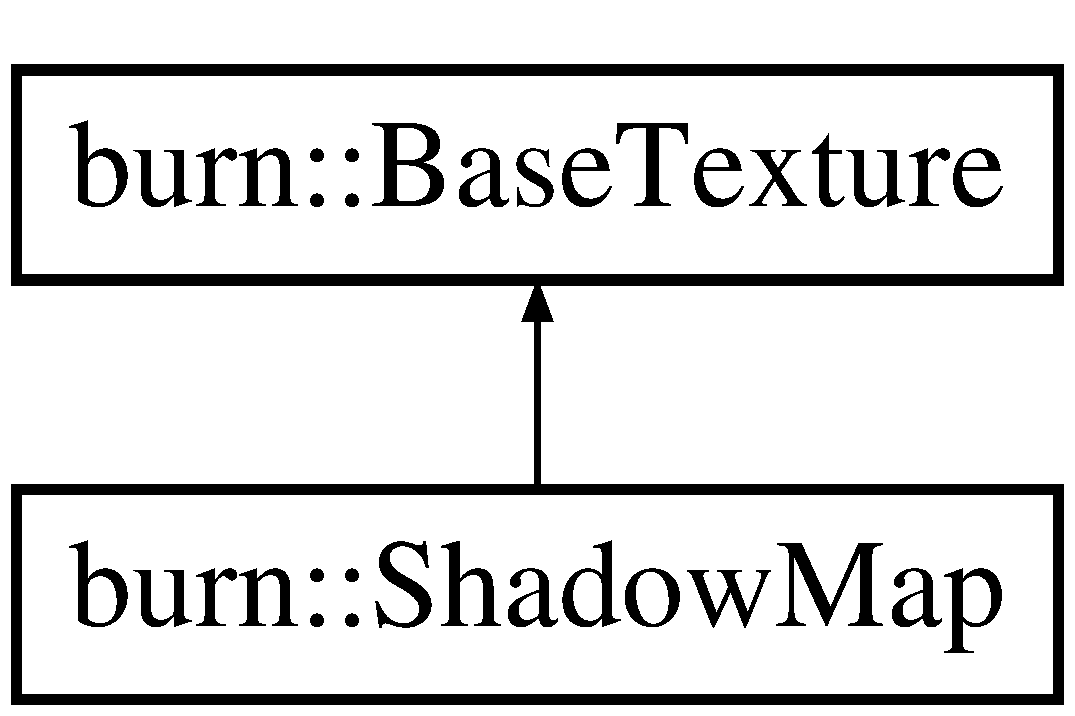
\includegraphics[height=2.000000cm]{classburn_1_1_shadow_map}
\end{center}
\end{figure}
\subsection*{Public Types}
\begin{DoxyCompactItemize}
\item 
enum \hyperlink{classburn_1_1_shadow_map_a5bc770d75b5d4d1c8f755546d20266d1}{Resolution} \{ \\*
\hyperlink{classburn_1_1_shadow_map_a5bc770d75b5d4d1c8f755546d20266d1a17d1c1b7bfaa4110d50071a8dd7d303a}{V\-E\-R\-Y\-\_\-\-L\-O\-W} = 128, 
\hyperlink{classburn_1_1_shadow_map_a5bc770d75b5d4d1c8f755546d20266d1a018be58e430ad0d7a919b349f2940727}{L\-O\-W} = 256, 
\hyperlink{classburn_1_1_shadow_map_a5bc770d75b5d4d1c8f755546d20266d1a37e0bf0a3fa1cd16bbe7144d8ac9e169}{M\-E\-D\-I\-U\-M} = 512, 
\hyperlink{classburn_1_1_shadow_map_a5bc770d75b5d4d1c8f755546d20266d1a0f4c9ac68ca6faffa3ca9d7adeea6093}{H\-I\-G\-H} = 1024, 
\\*
\hyperlink{classburn_1_1_shadow_map_a5bc770d75b5d4d1c8f755546d20266d1a6efbce9ee6e8bb911e9558fd6f3b9ef2}{V\-E\-R\-Y\-\_\-\-H\-I\-G\-H} = 2048
 \}
\end{DoxyCompactItemize}
\subsection*{Public Member Functions}
\begin{DoxyCompactItemize}
\item 
\hyperlink{classburn_1_1_shadow_map_a86f8dc0f4c9000f5d8598ab6519e8de4}{Shadow\-Map} ()
\item 
\hyperlink{classburn_1_1_shadow_map_a167c53e4c4b82b664994d2505d1a3a11}{Shadow\-Map} (const \hyperlink{classburn_1_1_shadow_map}{Shadow\-Map} \&other)=delete
\item 
\hyperlink{classburn_1_1_shadow_map}{Shadow\-Map} \& \hyperlink{classburn_1_1_shadow_map_aac229703746b53fbf8099871b291a4ef}{operator=} (const \hyperlink{classburn_1_1_shadow_map}{Shadow\-Map} \&other)=delete
\item 
\hyperlink{classburn_1_1_shadow_map_a853fac8f91d057da02ce65ac2c5a5a7f}{$\sim$\-Shadow\-Map} ()
\item 
bool \hyperlink{classburn_1_1_shadow_map_ae1fff318e3b188b925f2bd898337fcad}{create} (const \hyperlink{classburn_1_1_shadow_map_a5bc770d75b5d4d1c8f755546d20266d1}{Resolution} \&resolution=\hyperlink{classburn_1_1_shadow_map_a5bc770d75b5d4d1c8f755546d20266d1a0f4c9ac68ca6faffa3ca9d7adeea6093}{H\-I\-G\-H})
\item 
void \hyperlink{classburn_1_1_shadow_map_a791a5b8c53c3e1d1e88cf8252d81af50}{clear} ()
\item 
void \hyperlink{classburn_1_1_shadow_map_ab8d3115d83d69d7eb4d358760f9ca43d}{bind\-As\-Rendertarget} () const 
\item 
bool \hyperlink{classburn_1_1_shadow_map_a06b9cd9e57cc3e5914c4d20d56f0655b}{is\-Created} () const 
\end{DoxyCompactItemize}
\subsection*{Additional Inherited Members}


\subsection{Member Enumeration Documentation}
\hypertarget{classburn_1_1_shadow_map_a5bc770d75b5d4d1c8f755546d20266d1}{\index{burn\-::\-Shadow\-Map@{burn\-::\-Shadow\-Map}!Resolution@{Resolution}}
\index{Resolution@{Resolution}!burn::ShadowMap@{burn\-::\-Shadow\-Map}}
\subsubsection[{Resolution}]{\setlength{\rightskip}{0pt plus 5cm}enum {\bf burn\-::\-Shadow\-Map\-::\-Resolution}}}\label{classburn_1_1_shadow_map_a5bc770d75b5d4d1c8f755546d20266d1}
\begin{Desc}
\item[Enumerator]\par
\begin{description}
\index{V\-E\-R\-Y\-\_\-\-L\-O\-W@{V\-E\-R\-Y\-\_\-\-L\-O\-W}!burn\-::\-Shadow\-Map@{burn\-::\-Shadow\-Map}}\index{burn\-::\-Shadow\-Map@{burn\-::\-Shadow\-Map}!V\-E\-R\-Y\-\_\-\-L\-O\-W@{V\-E\-R\-Y\-\_\-\-L\-O\-W}}\item[{\em 
\hypertarget{classburn_1_1_shadow_map_a5bc770d75b5d4d1c8f755546d20266d1a17d1c1b7bfaa4110d50071a8dd7d303a}{V\-E\-R\-Y\-\_\-\-L\-O\-W}\label{classburn_1_1_shadow_map_a5bc770d75b5d4d1c8f755546d20266d1a17d1c1b7bfaa4110d50071a8dd7d303a}
}]128x128 \index{L\-O\-W@{L\-O\-W}!burn\-::\-Shadow\-Map@{burn\-::\-Shadow\-Map}}\index{burn\-::\-Shadow\-Map@{burn\-::\-Shadow\-Map}!L\-O\-W@{L\-O\-W}}\item[{\em 
\hypertarget{classburn_1_1_shadow_map_a5bc770d75b5d4d1c8f755546d20266d1a018be58e430ad0d7a919b349f2940727}{L\-O\-W}\label{classburn_1_1_shadow_map_a5bc770d75b5d4d1c8f755546d20266d1a018be58e430ad0d7a919b349f2940727}
}]256x256 \index{M\-E\-D\-I\-U\-M@{M\-E\-D\-I\-U\-M}!burn\-::\-Shadow\-Map@{burn\-::\-Shadow\-Map}}\index{burn\-::\-Shadow\-Map@{burn\-::\-Shadow\-Map}!M\-E\-D\-I\-U\-M@{M\-E\-D\-I\-U\-M}}\item[{\em 
\hypertarget{classburn_1_1_shadow_map_a5bc770d75b5d4d1c8f755546d20266d1a37e0bf0a3fa1cd16bbe7144d8ac9e169}{M\-E\-D\-I\-U\-M}\label{classburn_1_1_shadow_map_a5bc770d75b5d4d1c8f755546d20266d1a37e0bf0a3fa1cd16bbe7144d8ac9e169}
}]512x512 \index{H\-I\-G\-H@{H\-I\-G\-H}!burn\-::\-Shadow\-Map@{burn\-::\-Shadow\-Map}}\index{burn\-::\-Shadow\-Map@{burn\-::\-Shadow\-Map}!H\-I\-G\-H@{H\-I\-G\-H}}\item[{\em 
\hypertarget{classburn_1_1_shadow_map_a5bc770d75b5d4d1c8f755546d20266d1a0f4c9ac68ca6faffa3ca9d7adeea6093}{H\-I\-G\-H}\label{classburn_1_1_shadow_map_a5bc770d75b5d4d1c8f755546d20266d1a0f4c9ac68ca6faffa3ca9d7adeea6093}
}]1024x1024 \index{V\-E\-R\-Y\-\_\-\-H\-I\-G\-H@{V\-E\-R\-Y\-\_\-\-H\-I\-G\-H}!burn\-::\-Shadow\-Map@{burn\-::\-Shadow\-Map}}\index{burn\-::\-Shadow\-Map@{burn\-::\-Shadow\-Map}!V\-E\-R\-Y\-\_\-\-H\-I\-G\-H@{V\-E\-R\-Y\-\_\-\-H\-I\-G\-H}}\item[{\em 
\hypertarget{classburn_1_1_shadow_map_a5bc770d75b5d4d1c8f755546d20266d1a6efbce9ee6e8bb911e9558fd6f3b9ef2}{V\-E\-R\-Y\-\_\-\-H\-I\-G\-H}\label{classburn_1_1_shadow_map_a5bc770d75b5d4d1c8f755546d20266d1a6efbce9ee6e8bb911e9558fd6f3b9ef2}
}]2048x2048 \end{description}
\end{Desc}


\subsection{Constructor \& Destructor Documentation}
\hypertarget{classburn_1_1_shadow_map_a86f8dc0f4c9000f5d8598ab6519e8de4}{\index{burn\-::\-Shadow\-Map@{burn\-::\-Shadow\-Map}!Shadow\-Map@{Shadow\-Map}}
\index{Shadow\-Map@{Shadow\-Map}!burn::ShadowMap@{burn\-::\-Shadow\-Map}}
\subsubsection[{Shadow\-Map}]{\setlength{\rightskip}{0pt plus 5cm}burn\-::\-Shadow\-Map\-::\-Shadow\-Map (
\begin{DoxyParamCaption}
{}
\end{DoxyParamCaption}
)}}\label{classburn_1_1_shadow_map_a86f8dc0f4c9000f5d8598ab6519e8de4}
\hypertarget{classburn_1_1_shadow_map_a167c53e4c4b82b664994d2505d1a3a11}{\index{burn\-::\-Shadow\-Map@{burn\-::\-Shadow\-Map}!Shadow\-Map@{Shadow\-Map}}
\index{Shadow\-Map@{Shadow\-Map}!burn::ShadowMap@{burn\-::\-Shadow\-Map}}
\subsubsection[{Shadow\-Map}]{\setlength{\rightskip}{0pt plus 5cm}burn\-::\-Shadow\-Map\-::\-Shadow\-Map (
\begin{DoxyParamCaption}
\item[{const {\bf Shadow\-Map} \&}]{other}
\end{DoxyParamCaption}
)\hspace{0.3cm}{\ttfamily [delete]}}}\label{classburn_1_1_shadow_map_a167c53e4c4b82b664994d2505d1a3a11}
\hypertarget{classburn_1_1_shadow_map_a853fac8f91d057da02ce65ac2c5a5a7f}{\index{burn\-::\-Shadow\-Map@{burn\-::\-Shadow\-Map}!$\sim$\-Shadow\-Map@{$\sim$\-Shadow\-Map}}
\index{$\sim$\-Shadow\-Map@{$\sim$\-Shadow\-Map}!burn::ShadowMap@{burn\-::\-Shadow\-Map}}
\subsubsection[{$\sim$\-Shadow\-Map}]{\setlength{\rightskip}{0pt plus 5cm}burn\-::\-Shadow\-Map\-::$\sim$\-Shadow\-Map (
\begin{DoxyParamCaption}
{}
\end{DoxyParamCaption}
)}}\label{classburn_1_1_shadow_map_a853fac8f91d057da02ce65ac2c5a5a7f}


\subsection{Member Function Documentation}
\hypertarget{classburn_1_1_shadow_map_ab8d3115d83d69d7eb4d358760f9ca43d}{\index{burn\-::\-Shadow\-Map@{burn\-::\-Shadow\-Map}!bind\-As\-Rendertarget@{bind\-As\-Rendertarget}}
\index{bind\-As\-Rendertarget@{bind\-As\-Rendertarget}!burn::ShadowMap@{burn\-::\-Shadow\-Map}}
\subsubsection[{bind\-As\-Rendertarget}]{\setlength{\rightskip}{0pt plus 5cm}void burn\-::\-Shadow\-Map\-::bind\-As\-Rendertarget (
\begin{DoxyParamCaption}
{}
\end{DoxyParamCaption}
) const}}\label{classburn_1_1_shadow_map_ab8d3115d83d69d7eb4d358760f9ca43d}
\hypertarget{classburn_1_1_shadow_map_a791a5b8c53c3e1d1e88cf8252d81af50}{\index{burn\-::\-Shadow\-Map@{burn\-::\-Shadow\-Map}!clear@{clear}}
\index{clear@{clear}!burn::ShadowMap@{burn\-::\-Shadow\-Map}}
\subsubsection[{clear}]{\setlength{\rightskip}{0pt plus 5cm}void burn\-::\-Shadow\-Map\-::clear (
\begin{DoxyParamCaption}
{}
\end{DoxyParamCaption}
)}}\label{classburn_1_1_shadow_map_a791a5b8c53c3e1d1e88cf8252d81af50}
\hypertarget{classburn_1_1_shadow_map_ae1fff318e3b188b925f2bd898337fcad}{\index{burn\-::\-Shadow\-Map@{burn\-::\-Shadow\-Map}!create@{create}}
\index{create@{create}!burn::ShadowMap@{burn\-::\-Shadow\-Map}}
\subsubsection[{create}]{\setlength{\rightskip}{0pt plus 5cm}bool burn\-::\-Shadow\-Map\-::create (
\begin{DoxyParamCaption}
\item[{const {\bf Resolution} \&}]{resolution = {\ttfamily {\bf H\-I\-G\-H}}}
\end{DoxyParamCaption}
)}}\label{classburn_1_1_shadow_map_ae1fff318e3b188b925f2bd898337fcad}
\hypertarget{classburn_1_1_shadow_map_a06b9cd9e57cc3e5914c4d20d56f0655b}{\index{burn\-::\-Shadow\-Map@{burn\-::\-Shadow\-Map}!is\-Created@{is\-Created}}
\index{is\-Created@{is\-Created}!burn::ShadowMap@{burn\-::\-Shadow\-Map}}
\subsubsection[{is\-Created}]{\setlength{\rightskip}{0pt plus 5cm}bool burn\-::\-Shadow\-Map\-::is\-Created (
\begin{DoxyParamCaption}
{}
\end{DoxyParamCaption}
) const}}\label{classburn_1_1_shadow_map_a06b9cd9e57cc3e5914c4d20d56f0655b}
\hypertarget{classburn_1_1_shadow_map_aac229703746b53fbf8099871b291a4ef}{\index{burn\-::\-Shadow\-Map@{burn\-::\-Shadow\-Map}!operator=@{operator=}}
\index{operator=@{operator=}!burn::ShadowMap@{burn\-::\-Shadow\-Map}}
\subsubsection[{operator=}]{\setlength{\rightskip}{0pt plus 5cm}{\bf Shadow\-Map}\& burn\-::\-Shadow\-Map\-::operator= (
\begin{DoxyParamCaption}
\item[{const {\bf Shadow\-Map} \&}]{other}
\end{DoxyParamCaption}
)\hspace{0.3cm}{\ttfamily [delete]}}}\label{classburn_1_1_shadow_map_aac229703746b53fbf8099871b291a4ef}


The documentation for this class was generated from the following file\-:\begin{DoxyCompactItemize}
\item 
include/\-Burngine/\-Graphics/\-Texture/\hyperlink{_shadow_map_8h}{Shadow\-Map.\-h}\end{DoxyCompactItemize}

\hypertarget{classburn_1_1_sky_box}{\section{burn\-:\-:Sky\-Box Class Reference}
\label{classburn_1_1_sky_box}\index{burn\-::\-Sky\-Box@{burn\-::\-Sky\-Box}}
}


{\ttfamily \#include $<$Sky\-Box.\-h$>$}

\subsection*{Public Member Functions}
\begin{DoxyCompactItemize}
\item 
\hyperlink{classburn_1_1_sky_box_a43918ed26a1a03a41c34dc76b3da52a1}{Sky\-Box} ()
\item 
\hyperlink{classburn_1_1_sky_box_ad9d9c8bc70ea6cc9c7e3bc88a2ce5c4e}{Sky\-Box} (const \hyperlink{classburn_1_1_sky_box}{Sky\-Box} \&other)
\item 
\hyperlink{classburn_1_1_sky_box}{Sky\-Box} \& \hyperlink{classburn_1_1_sky_box_afe7077120c512a6fd5c2823c014ff125}{operator=} (const \hyperlink{classburn_1_1_sky_box}{Sky\-Box} \&other)
\item 
void \hyperlink{classburn_1_1_sky_box_ad77620d575b71d071e88120f6b6e145e}{set\-Cube\-Map} (const \hyperlink{classburn_1_1_cube_map}{Cube\-Map} \&cube\-Map)
\item 
const \hyperlink{classburn_1_1_cube_map}{Cube\-Map} \& \hyperlink{classburn_1_1_sky_box_aa7ec0fde41d2c0ffeacb7cfc64c85b80}{get\-Cube\-Map} () const 
\item 
void \hyperlink{classburn_1_1_sky_box_a700e08af93b54c0fb23ad225d3e6be5c}{draw} ()
\end{DoxyCompactItemize}


\subsection{Constructor \& Destructor Documentation}
\hypertarget{classburn_1_1_sky_box_a43918ed26a1a03a41c34dc76b3da52a1}{\index{burn\-::\-Sky\-Box@{burn\-::\-Sky\-Box}!Sky\-Box@{Sky\-Box}}
\index{Sky\-Box@{Sky\-Box}!burn::SkyBox@{burn\-::\-Sky\-Box}}
\subsubsection[{Sky\-Box}]{\setlength{\rightskip}{0pt plus 5cm}burn\-::\-Sky\-Box\-::\-Sky\-Box (
\begin{DoxyParamCaption}
{}
\end{DoxyParamCaption}
)}}\label{classburn_1_1_sky_box_a43918ed26a1a03a41c34dc76b3da52a1}
\hypertarget{classburn_1_1_sky_box_ad9d9c8bc70ea6cc9c7e3bc88a2ce5c4e}{\index{burn\-::\-Sky\-Box@{burn\-::\-Sky\-Box}!Sky\-Box@{Sky\-Box}}
\index{Sky\-Box@{Sky\-Box}!burn::SkyBox@{burn\-::\-Sky\-Box}}
\subsubsection[{Sky\-Box}]{\setlength{\rightskip}{0pt plus 5cm}burn\-::\-Sky\-Box\-::\-Sky\-Box (
\begin{DoxyParamCaption}
\item[{const {\bf Sky\-Box} \&}]{other}
\end{DoxyParamCaption}
)}}\label{classburn_1_1_sky_box_ad9d9c8bc70ea6cc9c7e3bc88a2ce5c4e}


\subsection{Member Function Documentation}
\hypertarget{classburn_1_1_sky_box_a700e08af93b54c0fb23ad225d3e6be5c}{\index{burn\-::\-Sky\-Box@{burn\-::\-Sky\-Box}!draw@{draw}}
\index{draw@{draw}!burn::SkyBox@{burn\-::\-Sky\-Box}}
\subsubsection[{draw}]{\setlength{\rightskip}{0pt plus 5cm}void burn\-::\-Sky\-Box\-::draw (
\begin{DoxyParamCaption}
{}
\end{DoxyParamCaption}
)}}\label{classburn_1_1_sky_box_a700e08af93b54c0fb23ad225d3e6be5c}
\hypertarget{classburn_1_1_sky_box_aa7ec0fde41d2c0ffeacb7cfc64c85b80}{\index{burn\-::\-Sky\-Box@{burn\-::\-Sky\-Box}!get\-Cube\-Map@{get\-Cube\-Map}}
\index{get\-Cube\-Map@{get\-Cube\-Map}!burn::SkyBox@{burn\-::\-Sky\-Box}}
\subsubsection[{get\-Cube\-Map}]{\setlength{\rightskip}{0pt plus 5cm}const {\bf Cube\-Map}\& burn\-::\-Sky\-Box\-::get\-Cube\-Map (
\begin{DoxyParamCaption}
{}
\end{DoxyParamCaption}
) const}}\label{classburn_1_1_sky_box_aa7ec0fde41d2c0ffeacb7cfc64c85b80}
\hypertarget{classburn_1_1_sky_box_afe7077120c512a6fd5c2823c014ff125}{\index{burn\-::\-Sky\-Box@{burn\-::\-Sky\-Box}!operator=@{operator=}}
\index{operator=@{operator=}!burn::SkyBox@{burn\-::\-Sky\-Box}}
\subsubsection[{operator=}]{\setlength{\rightskip}{0pt plus 5cm}{\bf Sky\-Box}\& burn\-::\-Sky\-Box\-::operator= (
\begin{DoxyParamCaption}
\item[{const {\bf Sky\-Box} \&}]{other}
\end{DoxyParamCaption}
)}}\label{classburn_1_1_sky_box_afe7077120c512a6fd5c2823c014ff125}
\hypertarget{classburn_1_1_sky_box_ad77620d575b71d071e88120f6b6e145e}{\index{burn\-::\-Sky\-Box@{burn\-::\-Sky\-Box}!set\-Cube\-Map@{set\-Cube\-Map}}
\index{set\-Cube\-Map@{set\-Cube\-Map}!burn::SkyBox@{burn\-::\-Sky\-Box}}
\subsubsection[{set\-Cube\-Map}]{\setlength{\rightskip}{0pt plus 5cm}void burn\-::\-Sky\-Box\-::set\-Cube\-Map (
\begin{DoxyParamCaption}
\item[{const {\bf Cube\-Map} \&}]{cube\-Map}
\end{DoxyParamCaption}
)}}\label{classburn_1_1_sky_box_ad77620d575b71d071e88120f6b6e145e}


The documentation for this class was generated from the following file\-:\begin{DoxyCompactItemize}
\item 
include/\-Burngine/\-Graphics/\-Scene/\hyperlink{_sky_box_8h}{Sky\-Box.\-h}\end{DoxyCompactItemize}

\hypertarget{classburn_1_1_spot_light}{\section{burn\-:\-:Spot\-Light Class Reference}
\label{classburn_1_1_spot_light}\index{burn\-::\-Spot\-Light@{burn\-::\-Spot\-Light}}
}


{\ttfamily \#include $<$Spot\-Light.\-h$>$}

Inheritance diagram for burn\-:\-:Spot\-Light\-:\begin{figure}[H]
\begin{center}
\leavevmode
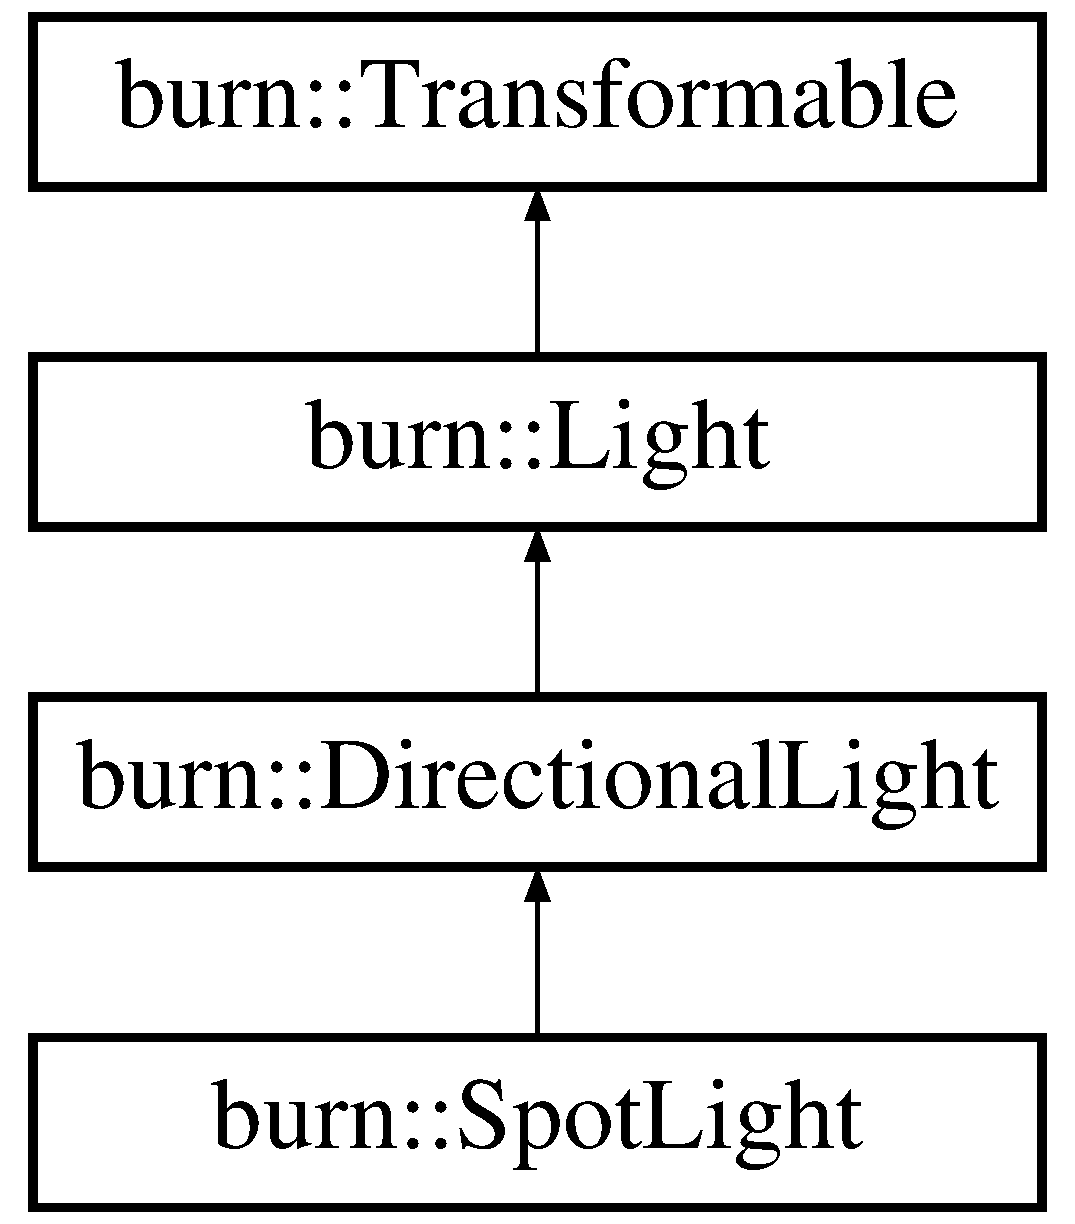
\includegraphics[height=4.000000cm]{classburn_1_1_spot_light}
\end{center}
\end{figure}
\subsection*{Public Member Functions}
\begin{DoxyCompactItemize}
\item 
\hyperlink{classburn_1_1_spot_light_ad22176a0896abbb3b0d56b521261b807}{Spot\-Light} ()
\item 
void \hyperlink{classburn_1_1_spot_light_a7fc9f81732923954a148f44518e2a01b}{set\-Cone\-Angle} (const float \&angle)
\item 
const float \& \hyperlink{classburn_1_1_spot_light_a07383c45e99954daad4afea3822914b5}{get\-Cone\-Angle} () const 
\item 
virtual void \hyperlink{classburn_1_1_spot_light_ab16ad5f4da0fe8fc9cdd07b2931259ee}{update\-Shadow\-Map} (const std\-::vector$<$ \hyperlink{classburn_1_1_scene_node}{Scene\-Node} $\ast$ $>$ \&nodes)
\end{DoxyCompactItemize}
\subsection*{Additional Inherited Members}


\subsection{Constructor \& Destructor Documentation}
\hypertarget{classburn_1_1_spot_light_ad22176a0896abbb3b0d56b521261b807}{\index{burn\-::\-Spot\-Light@{burn\-::\-Spot\-Light}!Spot\-Light@{Spot\-Light}}
\index{Spot\-Light@{Spot\-Light}!burn::SpotLight@{burn\-::\-Spot\-Light}}
\subsubsection[{Spot\-Light}]{\setlength{\rightskip}{0pt plus 5cm}burn\-::\-Spot\-Light\-::\-Spot\-Light (
\begin{DoxyParamCaption}
{}
\end{DoxyParamCaption}
)}}\label{classburn_1_1_spot_light_ad22176a0896abbb3b0d56b521261b807}


\subsection{Member Function Documentation}
\hypertarget{classburn_1_1_spot_light_a07383c45e99954daad4afea3822914b5}{\index{burn\-::\-Spot\-Light@{burn\-::\-Spot\-Light}!get\-Cone\-Angle@{get\-Cone\-Angle}}
\index{get\-Cone\-Angle@{get\-Cone\-Angle}!burn::SpotLight@{burn\-::\-Spot\-Light}}
\subsubsection[{get\-Cone\-Angle}]{\setlength{\rightskip}{0pt plus 5cm}const float\& burn\-::\-Spot\-Light\-::get\-Cone\-Angle (
\begin{DoxyParamCaption}
{}
\end{DoxyParamCaption}
) const}}\label{classburn_1_1_spot_light_a07383c45e99954daad4afea3822914b5}
\hypertarget{classburn_1_1_spot_light_a7fc9f81732923954a148f44518e2a01b}{\index{burn\-::\-Spot\-Light@{burn\-::\-Spot\-Light}!set\-Cone\-Angle@{set\-Cone\-Angle}}
\index{set\-Cone\-Angle@{set\-Cone\-Angle}!burn::SpotLight@{burn\-::\-Spot\-Light}}
\subsubsection[{set\-Cone\-Angle}]{\setlength{\rightskip}{0pt plus 5cm}void burn\-::\-Spot\-Light\-::set\-Cone\-Angle (
\begin{DoxyParamCaption}
\item[{const float \&}]{angle}
\end{DoxyParamCaption}
)}}\label{classburn_1_1_spot_light_a7fc9f81732923954a148f44518e2a01b}
\hypertarget{classburn_1_1_spot_light_ab16ad5f4da0fe8fc9cdd07b2931259ee}{\index{burn\-::\-Spot\-Light@{burn\-::\-Spot\-Light}!update\-Shadow\-Map@{update\-Shadow\-Map}}
\index{update\-Shadow\-Map@{update\-Shadow\-Map}!burn::SpotLight@{burn\-::\-Spot\-Light}}
\subsubsection[{update\-Shadow\-Map}]{\setlength{\rightskip}{0pt plus 5cm}virtual void burn\-::\-Spot\-Light\-::update\-Shadow\-Map (
\begin{DoxyParamCaption}
\item[{const std\-::vector$<$ {\bf Scene\-Node} $\ast$ $>$ \&}]{nodes}
\end{DoxyParamCaption}
)\hspace{0.3cm}{\ttfamily [virtual]}}}\label{classburn_1_1_spot_light_ab16ad5f4da0fe8fc9cdd07b2931259ee}


Reimplemented from \hyperlink{classburn_1_1_directional_light_a84eb0090ded76e9f73d351ff87a54795}{burn\-::\-Directional\-Light}.



The documentation for this class was generated from the following file\-:\begin{DoxyCompactItemize}
\item 
include/\-Burngine/\-Graphics/\-Scene/\hyperlink{_spot_light_8h}{Spot\-Light.\-h}\end{DoxyCompactItemize}

\hypertarget{classburn_1_1_static_mesh_node}{\section{burn\-:\-:Static\-Mesh\-Node Class Reference}
\label{classburn_1_1_static_mesh_node}\index{burn\-::\-Static\-Mesh\-Node@{burn\-::\-Static\-Mesh\-Node}}
}


{\ttfamily \#include $<$Static\-Mesh\-Node.\-h$>$}

Inheritance diagram for burn\-:\-:Static\-Mesh\-Node\-:\begin{figure}[H]
\begin{center}
\leavevmode
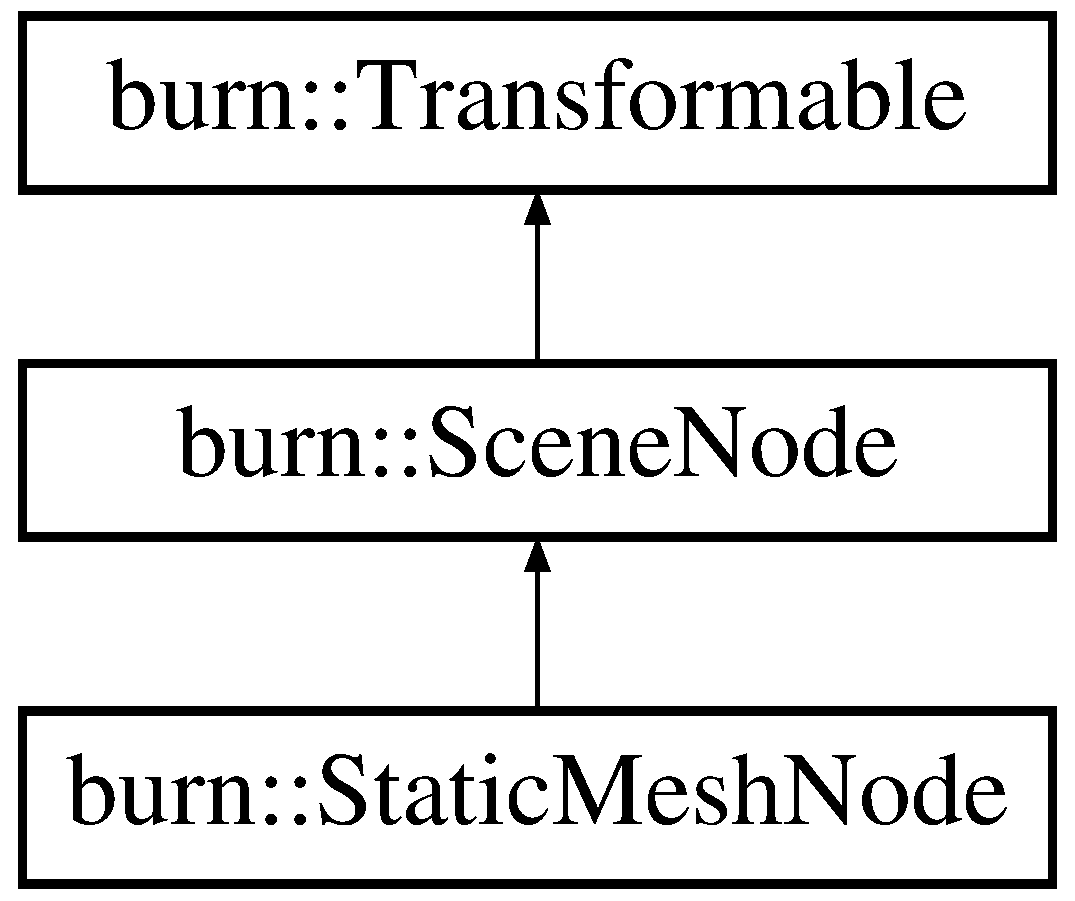
\includegraphics[height=3.000000cm]{classburn_1_1_static_mesh_node}
\end{center}
\end{figure}
\subsection*{Public Member Functions}
\begin{DoxyCompactItemize}
\item 
\hyperlink{classburn_1_1_static_mesh_node_a051ef5fe091cf8e93cc4dd1bae753cbd}{Static\-Mesh\-Node} ()
\item 
\hyperlink{classburn_1_1_static_mesh_node_a68e00b329768da175ee153c46069364e}{$\sim$\-Static\-Mesh\-Node} ()
\item 
void \hyperlink{classburn_1_1_static_mesh_node_af78ecebdfd7c25997caf35ef4ebecdfb}{set\-Mesh} (const \hyperlink{classburn_1_1_mesh}{Mesh} \&mesh)
\item 
const \hyperlink{classburn_1_1_mesh}{Mesh} \& \hyperlink{classburn_1_1_static_mesh_node_ad269a91df547f3a3092d193e4210e081}{get\-Mesh} () const 
\item 
virtual void \hyperlink{classburn_1_1_static_mesh_node_a7ff88bee9757061b0393ae5324e7989b}{draw} (\hyperlink{classburn_1_1_camera}{Camera} $\ast$cam=nullptr)
\end{DoxyCompactItemize}
\subsection*{Additional Inherited Members}


\subsection{Constructor \& Destructor Documentation}
\hypertarget{classburn_1_1_static_mesh_node_a051ef5fe091cf8e93cc4dd1bae753cbd}{\index{burn\-::\-Static\-Mesh\-Node@{burn\-::\-Static\-Mesh\-Node}!Static\-Mesh\-Node@{Static\-Mesh\-Node}}
\index{Static\-Mesh\-Node@{Static\-Mesh\-Node}!burn::StaticMeshNode@{burn\-::\-Static\-Mesh\-Node}}
\subsubsection[{Static\-Mesh\-Node}]{\setlength{\rightskip}{0pt plus 5cm}burn\-::\-Static\-Mesh\-Node\-::\-Static\-Mesh\-Node (
\begin{DoxyParamCaption}
{}
\end{DoxyParamCaption}
)}}\label{classburn_1_1_static_mesh_node_a051ef5fe091cf8e93cc4dd1bae753cbd}
\hypertarget{classburn_1_1_static_mesh_node_a68e00b329768da175ee153c46069364e}{\index{burn\-::\-Static\-Mesh\-Node@{burn\-::\-Static\-Mesh\-Node}!$\sim$\-Static\-Mesh\-Node@{$\sim$\-Static\-Mesh\-Node}}
\index{$\sim$\-Static\-Mesh\-Node@{$\sim$\-Static\-Mesh\-Node}!burn::StaticMeshNode@{burn\-::\-Static\-Mesh\-Node}}
\subsubsection[{$\sim$\-Static\-Mesh\-Node}]{\setlength{\rightskip}{0pt plus 5cm}burn\-::\-Static\-Mesh\-Node\-::$\sim$\-Static\-Mesh\-Node (
\begin{DoxyParamCaption}
{}
\end{DoxyParamCaption}
)}}\label{classburn_1_1_static_mesh_node_a68e00b329768da175ee153c46069364e}


\subsection{Member Function Documentation}
\hypertarget{classburn_1_1_static_mesh_node_a7ff88bee9757061b0393ae5324e7989b}{\index{burn\-::\-Static\-Mesh\-Node@{burn\-::\-Static\-Mesh\-Node}!draw@{draw}}
\index{draw@{draw}!burn::StaticMeshNode@{burn\-::\-Static\-Mesh\-Node}}
\subsubsection[{draw}]{\setlength{\rightskip}{0pt plus 5cm}void burn\-::\-Static\-Mesh\-Node\-::draw (
\begin{DoxyParamCaption}
\item[{{\bf Camera} $\ast$}]{cam = {\ttfamily nullptr}}
\end{DoxyParamCaption}
)\hspace{0.3cm}{\ttfamily [virtual]}}}\label{classburn_1_1_static_mesh_node_a7ff88bee9757061b0393ae5324e7989b}


Implements \hyperlink{classburn_1_1_scene_node_adcea597571e59f15421c7a9ae0bfdbc3}{burn\-::\-Scene\-Node}.

\hypertarget{classburn_1_1_static_mesh_node_ad269a91df547f3a3092d193e4210e081}{\index{burn\-::\-Static\-Mesh\-Node@{burn\-::\-Static\-Mesh\-Node}!get\-Mesh@{get\-Mesh}}
\index{get\-Mesh@{get\-Mesh}!burn::StaticMeshNode@{burn\-::\-Static\-Mesh\-Node}}
\subsubsection[{get\-Mesh}]{\setlength{\rightskip}{0pt plus 5cm}const {\bf Mesh} \& burn\-::\-Static\-Mesh\-Node\-::get\-Mesh (
\begin{DoxyParamCaption}
{}
\end{DoxyParamCaption}
) const}}\label{classburn_1_1_static_mesh_node_ad269a91df547f3a3092d193e4210e081}
\hypertarget{classburn_1_1_static_mesh_node_af78ecebdfd7c25997caf35ef4ebecdfb}{\index{burn\-::\-Static\-Mesh\-Node@{burn\-::\-Static\-Mesh\-Node}!set\-Mesh@{set\-Mesh}}
\index{set\-Mesh@{set\-Mesh}!burn::StaticMeshNode@{burn\-::\-Static\-Mesh\-Node}}
\subsubsection[{set\-Mesh}]{\setlength{\rightskip}{0pt plus 5cm}void burn\-::\-Static\-Mesh\-Node\-::set\-Mesh (
\begin{DoxyParamCaption}
\item[{const {\bf Mesh} \&}]{mesh}
\end{DoxyParamCaption}
)}}\label{classburn_1_1_static_mesh_node_af78ecebdfd7c25997caf35ef4ebecdfb}


The documentation for this class was generated from the following files\-:\begin{DoxyCompactItemize}
\item 
include/\-Burngine/\-Graphics/\hyperlink{_static_mesh_node_8h}{Static\-Mesh\-Node.\-h}\item 
include/\-Burngine/\-Graphics/\hyperlink{_static_mesh_node_8cpp}{Static\-Mesh\-Node.\-cpp}\end{DoxyCompactItemize}

\hypertarget{classburn_1_1_string}{\section{burn\-:\-:String Class Reference}
\label{classburn_1_1_string}\index{burn\-::\-String@{burn\-::\-String}}
}


Utility string class that automatically handles conversions between types and encodings.  




{\ttfamily \#include $<$String.\-h$>$}

\subsection*{Public Types}
\begin{DoxyCompactItemize}
\item 
typedef std\-::basic\-\_\-string\\*
$<$ \hyperlink{namespaceburn_ab40b09022209bd449d317c1f0e95356b}{Uint32} $>$\-::iterator \hyperlink{classburn_1_1_string_a84bf349f5c87cfcca666afade353be83}{Iterator}
\begin{DoxyCompactList}\small\item\em Iterator type. \end{DoxyCompactList}\item 
typedef std\-::basic\-\_\-string\\*
$<$ \hyperlink{namespaceburn_ab40b09022209bd449d317c1f0e95356b}{Uint32} $>$\-::const\-\_\-iterator \hyperlink{classburn_1_1_string_a323849432c1bf90a416b1afceb37e1ff}{Const\-Iterator}
\begin{DoxyCompactList}\small\item\em Constant iterator type. \end{DoxyCompactList}\end{DoxyCompactItemize}
\subsection*{Public Member Functions}
\begin{DoxyCompactItemize}
\item 
\hyperlink{classburn_1_1_string_a6c2a9c183185a6517d3939ac4ae356bb}{String} ()
\begin{DoxyCompactList}\small\item\em Default constructor. \end{DoxyCompactList}\item 
\hyperlink{classburn_1_1_string_af51a79a81210029650e8ba192b4aa997}{String} (char ansi\-Char, const std\-::locale \&locale=std\-::locale())
\begin{DoxyCompactList}\small\item\em Construct from a single A\-N\-S\-I character and a locale. \end{DoxyCompactList}\item 
\hyperlink{classburn_1_1_string_a008cbc555418be30aaf5a69c0a5c6fb9}{String} (wchar\-\_\-t wide\-Char)
\begin{DoxyCompactList}\small\item\em Construct from single wide character. \end{DoxyCompactList}\item 
\hyperlink{classburn_1_1_string_a7bcbce96cf6e89552855dae02561db27}{String} (\hyperlink{namespaceburn_ab40b09022209bd449d317c1f0e95356b}{Uint32} utf32\-Char)
\begin{DoxyCompactList}\small\item\em Construct from single U\-T\-F-\/32 character. \end{DoxyCompactList}\item 
\hyperlink{classburn_1_1_string_aca30936fde5294c14d5ce855823e03e0}{String} (const char $\ast$ansi\-String, const std\-::locale \&locale=std\-::locale())
\begin{DoxyCompactList}\small\item\em Construct from a null-\/terminated C-\/style A\-N\-S\-I string and a locale. \end{DoxyCompactList}\item 
\hyperlink{classburn_1_1_string_a5e45efc34aa57def453fbd6f995dbac4}{String} (const std\-::string \&ansi\-String, const std\-::locale \&locale=std\-::locale())
\begin{DoxyCompactList}\small\item\em Construct from an A\-N\-S\-I string and a locale. \end{DoxyCompactList}\item 
\hyperlink{classburn_1_1_string_af4715424b8beb05efa209a332e2ffd77}{String} (const wchar\-\_\-t $\ast$wide\-String)
\begin{DoxyCompactList}\small\item\em Construct from null-\/terminated C-\/style wide string. \end{DoxyCompactList}\item 
\hyperlink{classburn_1_1_string_a40658c80f170163c4b7294d36c4e458c}{String} (const std\-::wstring \&wide\-String)
\begin{DoxyCompactList}\small\item\em Construct from a wide string. \end{DoxyCompactList}\item 
\hyperlink{classburn_1_1_string_aed7c164cd06ccd741917dcfb717dfdd3}{String} (const \hyperlink{namespaceburn_ab40b09022209bd449d317c1f0e95356b}{Uint32} $\ast$utf32\-String)
\begin{DoxyCompactList}\small\item\em Construct from a null-\/terminated C-\/style U\-T\-F-\/32 string. \end{DoxyCompactList}\item 
\hyperlink{classburn_1_1_string_a6352b76b09fb99657b2a56f557941596}{String} (const std\-::basic\-\_\-string$<$ \hyperlink{namespaceburn_ab40b09022209bd449d317c1f0e95356b}{Uint32} $>$ \&utf32\-String)
\begin{DoxyCompactList}\small\item\em Construct from an U\-T\-F-\/32 string. \end{DoxyCompactList}\item 
\hyperlink{classburn_1_1_string_a77d71a82e074ec6a48087026aadfa36d}{String} (const \hyperlink{classburn_1_1_string}{String} \&copy)
\begin{DoxyCompactList}\small\item\em Copy constructor. \end{DoxyCompactList}\item 
\hyperlink{classburn_1_1_string_a1b2475781bec48ff43e28e986cb2eed8}{operator std\-::string} () const 
\begin{DoxyCompactList}\small\item\em Implicit cast operator to std\-::string (A\-N\-S\-I string) \end{DoxyCompactList}\item 
\hyperlink{classburn_1_1_string_aaf1ce104de7a958b6ed9575fb10e5c9f}{operator std\-::wstring} () const 
\begin{DoxyCompactList}\small\item\em Implicit cast operator to std\-::wstring (wide string) \end{DoxyCompactList}\item 
std\-::string \hyperlink{classburn_1_1_string_a1a11e9382f744cadaea480a3b70dc1ef}{to\-Ansi\-String} (const std\-::locale \&locale=std\-::locale()) const 
\begin{DoxyCompactList}\small\item\em Convert the unicode string to an A\-N\-S\-I string. \end{DoxyCompactList}\item 
std\-::wstring \hyperlink{classburn_1_1_string_abcaa6ebd5743cc885c15577ca08a62f2}{to\-Wide\-String} () const 
\begin{DoxyCompactList}\small\item\em Convert the unicode string to a wide string. \end{DoxyCompactList}\item 
\hyperlink{classburn_1_1_string}{String} \& \hyperlink{classburn_1_1_string_abbd178f658f0c6951054381013443f05}{operator=} (const \hyperlink{classburn_1_1_string}{String} \&right)
\begin{DoxyCompactList}\small\item\em Overload of assignment operator. \end{DoxyCompactList}\item 
\hyperlink{classburn_1_1_string}{String} \& \hyperlink{classburn_1_1_string_a6410f053b7bab08458e4d0789de3b5f7}{operator+=} (const \hyperlink{classburn_1_1_string}{String} \&right)
\begin{DoxyCompactList}\small\item\em Overload of += operator to append an U\-T\-F-\/32 string. \end{DoxyCompactList}\item 
\hyperlink{namespaceburn_ab40b09022209bd449d317c1f0e95356b}{Uint32} \hyperlink{classburn_1_1_string_ae103536549b576275ea04978e80f7372}{operator\mbox{[}$\,$\mbox{]}} (std\-::size\-\_\-t index) const 
\begin{DoxyCompactList}\small\item\em Overload of \mbox{[}\mbox{]} operator to access a character by its position. \end{DoxyCompactList}\item 
\hyperlink{namespaceburn_ab40b09022209bd449d317c1f0e95356b}{Uint32} \& \hyperlink{classburn_1_1_string_acc1f80f7268b5465d7a3a49cf7927272}{operator\mbox{[}$\,$\mbox{]}} (std\-::size\-\_\-t index)
\begin{DoxyCompactList}\small\item\em Overload of \mbox{[}\mbox{]} operator to access a character by its position. \end{DoxyCompactList}\item 
void \hyperlink{classburn_1_1_string_a17785eac89172fb6a86a6ff2018317d1}{clear} ()
\begin{DoxyCompactList}\small\item\em Clear the string. \end{DoxyCompactList}\item 
std\-::size\-\_\-t \hyperlink{classburn_1_1_string_a2551be01727cdd3c82671c49923e7ba0}{get\-Size} () const 
\begin{DoxyCompactList}\small\item\em Get the size of the string. \end{DoxyCompactList}\item 
bool \hyperlink{classburn_1_1_string_a5723443c8aa152bb6451252dabec7640}{is\-Empty} () const 
\begin{DoxyCompactList}\small\item\em Check whether the string is empty or not. \end{DoxyCompactList}\item 
void \hyperlink{classburn_1_1_string_aa82d8a0adc6f39448835cca4ae81c5ef}{erase} (std\-::size\-\_\-t position, std\-::size\-\_\-t count=1)
\begin{DoxyCompactList}\small\item\em Erase one or more characters from the string. \end{DoxyCompactList}\item 
void \hyperlink{classburn_1_1_string_a106dfd5ead837b8908142289dfaf531c}{insert} (std\-::size\-\_\-t position, const \hyperlink{classburn_1_1_string}{String} \&str)
\begin{DoxyCompactList}\small\item\em Insert one or more characters into the string. \end{DoxyCompactList}\item 
std\-::size\-\_\-t \hyperlink{classburn_1_1_string_add934aa6197f730de79445a18942a5fc}{find} (const \hyperlink{classburn_1_1_string}{String} \&str, std\-::size\-\_\-t start=0) const 
\begin{DoxyCompactList}\small\item\em Find a sequence of one or more characters in the string. \end{DoxyCompactList}\item 
const \hyperlink{namespaceburn_ab40b09022209bd449d317c1f0e95356b}{Uint32} $\ast$ \hyperlink{classburn_1_1_string_ac640bcb974455719360ccd4ff8989acf}{get\-Data} () const 
\begin{DoxyCompactList}\small\item\em Get a pointer to the C-\/style array of characters. \end{DoxyCompactList}\item 
\hyperlink{classburn_1_1_string_a84bf349f5c87cfcca666afade353be83}{Iterator} \hyperlink{classburn_1_1_string_ab0226b4c722bb95fc14e4b3fe693962e}{begin} ()
\begin{DoxyCompactList}\small\item\em Return an iterator to the beginning of the string. \end{DoxyCompactList}\item 
\hyperlink{classburn_1_1_string_a323849432c1bf90a416b1afceb37e1ff}{Const\-Iterator} \hyperlink{classburn_1_1_string_a7d4e74862db2d1c981a38b647b1ffba3}{begin} () const 
\begin{DoxyCompactList}\small\item\em Return an iterator to the beginning of the string. \end{DoxyCompactList}\item 
\hyperlink{classburn_1_1_string_a84bf349f5c87cfcca666afade353be83}{Iterator} \hyperlink{classburn_1_1_string_a263b6da9d3dcaed30ae4e6874c2b681e}{end} ()
\begin{DoxyCompactList}\small\item\em Return an iterator to the beginning of the string. \end{DoxyCompactList}\item 
\hyperlink{classburn_1_1_string_a323849432c1bf90a416b1afceb37e1ff}{Const\-Iterator} \hyperlink{classburn_1_1_string_a5e3b0982ddcdf5812783caf9726c3830}{end} () const 
\begin{DoxyCompactList}\small\item\em Return an iterator to the beginning of the string. \end{DoxyCompactList}\end{DoxyCompactItemize}
\subsection*{Static Public Attributes}
\begin{DoxyCompactItemize}
\item 
static const std\-::size\-\_\-t \hyperlink{classburn_1_1_string_adcc78caaf445a41121006dfbd91f1cdc}{Invalid\-Pos}
\begin{DoxyCompactList}\small\item\em Represents an invalid position in the string. \end{DoxyCompactList}\end{DoxyCompactItemize}
\subsection*{Friends}
\begin{DoxyCompactItemize}
\item 
\hyperlink{_export_8h_a5040e4252a67428f940a23fa9dbfec7b}{B\-U\-R\-N\-G\-I\-N\-E\-\_\-\-A\-P\-I} bool \hyperlink{classburn_1_1_string_acd3ff7c79fe5f694755cde868e0b953a}{operator==} (const \hyperlink{classburn_1_1_string}{String} \&left, const \hyperlink{classburn_1_1_string}{String} \&right)
\item 
\hyperlink{_export_8h_a5040e4252a67428f940a23fa9dbfec7b}{B\-U\-R\-N\-G\-I\-N\-E\-\_\-\-A\-P\-I} bool \hyperlink{classburn_1_1_string_a4a8fbb4493570c7025b3ddf4d6577295}{operator$<$} (const \hyperlink{classburn_1_1_string}{String} \&left, const \hyperlink{classburn_1_1_string}{String} \&right)
\end{DoxyCompactItemize}
\subsection*{Related Functions}
(Note that these are not member functions.) \begin{DoxyCompactItemize}
\item 
\hyperlink{_export_8h_a5040e4252a67428f940a23fa9dbfec7b}{B\-U\-R\-N\-G\-I\-N\-E\-\_\-\-A\-P\-I} bool \hyperlink{classburn_1_1_string_acd3ff7c79fe5f694755cde868e0b953a}{operator==} (const \hyperlink{classburn_1_1_string}{String} \&left, const \hyperlink{classburn_1_1_string}{String} \&right)
\begin{DoxyCompactList}\small\item\em Overload of == operator to compare two U\-T\-F-\/32 strings. \end{DoxyCompactList}\item 
\hyperlink{_export_8h_a5040e4252a67428f940a23fa9dbfec7b}{B\-U\-R\-N\-G\-I\-N\-E\-\_\-\-A\-P\-I} bool \hyperlink{classburn_1_1_string_aa699fb80a7e683001cc381a904adf7c7}{operator!=} (const \hyperlink{classburn_1_1_string}{String} \&left, const \hyperlink{classburn_1_1_string}{String} \&right)
\begin{DoxyCompactList}\small\item\em Overload of != operator to compare two U\-T\-F-\/32 strings. \end{DoxyCompactList}\item 
\hyperlink{_export_8h_a5040e4252a67428f940a23fa9dbfec7b}{B\-U\-R\-N\-G\-I\-N\-E\-\_\-\-A\-P\-I} bool \hyperlink{classburn_1_1_string_a4a8fbb4493570c7025b3ddf4d6577295}{operator$<$} (const \hyperlink{classburn_1_1_string}{String} \&left, const \hyperlink{classburn_1_1_string}{String} \&right)
\begin{DoxyCompactList}\small\item\em Overload of $<$ operator to compare two U\-T\-F-\/32 strings. \end{DoxyCompactList}\item 
\hyperlink{_export_8h_a5040e4252a67428f940a23fa9dbfec7b}{B\-U\-R\-N\-G\-I\-N\-E\-\_\-\-A\-P\-I} bool \hyperlink{classburn_1_1_string_a11d2287c52543833b39574735b4a0a52}{operator$>$} (const \hyperlink{classburn_1_1_string}{String} \&left, const \hyperlink{classburn_1_1_string}{String} \&right)
\begin{DoxyCompactList}\small\item\em Overload of $>$ operator to compare two U\-T\-F-\/32 strings. \end{DoxyCompactList}\item 
\hyperlink{_export_8h_a5040e4252a67428f940a23fa9dbfec7b}{B\-U\-R\-N\-G\-I\-N\-E\-\_\-\-A\-P\-I} bool \hyperlink{classburn_1_1_string_a316ac376afd496075145d92318e04ab8}{operator$<$=} (const \hyperlink{classburn_1_1_string}{String} \&left, const \hyperlink{classburn_1_1_string}{String} \&right)
\begin{DoxyCompactList}\small\item\em Overload of $<$= operator to compare two U\-T\-F-\/32 strings. \end{DoxyCompactList}\item 
\hyperlink{_export_8h_a5040e4252a67428f940a23fa9dbfec7b}{B\-U\-R\-N\-G\-I\-N\-E\-\_\-\-A\-P\-I} bool \hyperlink{classburn_1_1_string_adf45e6d139d925c476c5dcabfa676bba}{operator$>$=} (const \hyperlink{classburn_1_1_string}{String} \&left, const \hyperlink{classburn_1_1_string}{String} \&right)
\begin{DoxyCompactList}\small\item\em Overload of $>$= operator to compare two U\-T\-F-\/32 strings. \end{DoxyCompactList}\item 
\hyperlink{_export_8h_a5040e4252a67428f940a23fa9dbfec7b}{B\-U\-R\-N\-G\-I\-N\-E\-\_\-\-A\-P\-I} \hyperlink{classburn_1_1_string}{String} \hyperlink{classburn_1_1_string_aeea4a77b7b5306c4632804a6e80a9f28}{operator+} (const \hyperlink{classburn_1_1_string}{String} \&left, const \hyperlink{classburn_1_1_string}{String} \&right)
\begin{DoxyCompactList}\small\item\em Overload of binary + operator to concatenate two strings. \end{DoxyCompactList}\end{DoxyCompactItemize}


\subsection{Detailed Description}
Utility string class that automatically handles conversions between types and encodings. 

\subsection{Member Typedef Documentation}
\hypertarget{classburn_1_1_string_a323849432c1bf90a416b1afceb37e1ff}{\index{burn\-::\-String@{burn\-::\-String}!Const\-Iterator@{Const\-Iterator}}
\index{Const\-Iterator@{Const\-Iterator}!burn::String@{burn\-::\-String}}
\subsubsection[{Const\-Iterator}]{\setlength{\rightskip}{0pt plus 5cm}typedef std\-::basic\-\_\-string$<${\bf Uint32}$>$\-::const\-\_\-iterator {\bf burn\-::\-String\-::\-Const\-Iterator}}}\label{classburn_1_1_string_a323849432c1bf90a416b1afceb37e1ff}


Constant iterator type. 

\hypertarget{classburn_1_1_string_a84bf349f5c87cfcca666afade353be83}{\index{burn\-::\-String@{burn\-::\-String}!Iterator@{Iterator}}
\index{Iterator@{Iterator}!burn::String@{burn\-::\-String}}
\subsubsection[{Iterator}]{\setlength{\rightskip}{0pt plus 5cm}typedef std\-::basic\-\_\-string$<${\bf Uint32}$>$\-::iterator {\bf burn\-::\-String\-::\-Iterator}}}\label{classburn_1_1_string_a84bf349f5c87cfcca666afade353be83}


Iterator type. 



\subsection{Constructor \& Destructor Documentation}
\hypertarget{classburn_1_1_string_a6c2a9c183185a6517d3939ac4ae356bb}{\index{burn\-::\-String@{burn\-::\-String}!String@{String}}
\index{String@{String}!burn::String@{burn\-::\-String}}
\subsubsection[{String}]{\setlength{\rightskip}{0pt plus 5cm}burn\-::\-String\-::\-String (
\begin{DoxyParamCaption}
{}
\end{DoxyParamCaption}
)}}\label{classburn_1_1_string_a6c2a9c183185a6517d3939ac4ae356bb}


Default constructor. 

This constructor creates an empty string. \hypertarget{classburn_1_1_string_af51a79a81210029650e8ba192b4aa997}{\index{burn\-::\-String@{burn\-::\-String}!String@{String}}
\index{String@{String}!burn::String@{burn\-::\-String}}
\subsubsection[{String}]{\setlength{\rightskip}{0pt plus 5cm}burn\-::\-String\-::\-String (
\begin{DoxyParamCaption}
\item[{char}]{ansi\-Char, }
\item[{const std\-::locale \&}]{locale = {\ttfamily std\-:\-:locale()}}
\end{DoxyParamCaption}
)}}\label{classburn_1_1_string_af51a79a81210029650e8ba192b4aa997}


Construct from a single A\-N\-S\-I character and a locale. 

The source character is converted to U\-T\-F-\/32 according to the given locale.


\begin{DoxyParams}{Parameters}
{\em ansi\-Char} & A\-N\-S\-I character to convert \\
\hline
{\em locale} & Locale to use for conversion \\
\hline
\end{DoxyParams}
\hypertarget{classburn_1_1_string_a008cbc555418be30aaf5a69c0a5c6fb9}{\index{burn\-::\-String@{burn\-::\-String}!String@{String}}
\index{String@{String}!burn::String@{burn\-::\-String}}
\subsubsection[{String}]{\setlength{\rightskip}{0pt plus 5cm}burn\-::\-String\-::\-String (
\begin{DoxyParamCaption}
\item[{wchar\-\_\-t}]{wide\-Char}
\end{DoxyParamCaption}
)}}\label{classburn_1_1_string_a008cbc555418be30aaf5a69c0a5c6fb9}


Construct from single wide character. 


\begin{DoxyParams}{Parameters}
{\em wide\-Char} & Wide character to convert \\
\hline
\end{DoxyParams}
\hypertarget{classburn_1_1_string_a7bcbce96cf6e89552855dae02561db27}{\index{burn\-::\-String@{burn\-::\-String}!String@{String}}
\index{String@{String}!burn::String@{burn\-::\-String}}
\subsubsection[{String}]{\setlength{\rightskip}{0pt plus 5cm}burn\-::\-String\-::\-String (
\begin{DoxyParamCaption}
\item[{{\bf Uint32}}]{utf32\-Char}
\end{DoxyParamCaption}
)}}\label{classburn_1_1_string_a7bcbce96cf6e89552855dae02561db27}


Construct from single U\-T\-F-\/32 character. 


\begin{DoxyParams}{Parameters}
{\em utf32\-Char} & U\-T\-F-\/32 character to convert \\
\hline
\end{DoxyParams}
\hypertarget{classburn_1_1_string_aca30936fde5294c14d5ce855823e03e0}{\index{burn\-::\-String@{burn\-::\-String}!String@{String}}
\index{String@{String}!burn::String@{burn\-::\-String}}
\subsubsection[{String}]{\setlength{\rightskip}{0pt plus 5cm}burn\-::\-String\-::\-String (
\begin{DoxyParamCaption}
\item[{const char $\ast$}]{ansi\-String, }
\item[{const std\-::locale \&}]{locale = {\ttfamily std\-:\-:locale()}}
\end{DoxyParamCaption}
)}}\label{classburn_1_1_string_aca30936fde5294c14d5ce855823e03e0}


Construct from a null-\/terminated C-\/style A\-N\-S\-I string and a locale. 

The source string is converted to U\-T\-F-\/32 according to the given locale.


\begin{DoxyParams}{Parameters}
{\em ansi\-String} & A\-N\-S\-I string to convert \\
\hline
{\em locale} & Locale to use for conversion \\
\hline
\end{DoxyParams}
\hypertarget{classburn_1_1_string_a5e45efc34aa57def453fbd6f995dbac4}{\index{burn\-::\-String@{burn\-::\-String}!String@{String}}
\index{String@{String}!burn::String@{burn\-::\-String}}
\subsubsection[{String}]{\setlength{\rightskip}{0pt plus 5cm}burn\-::\-String\-::\-String (
\begin{DoxyParamCaption}
\item[{const std\-::string \&}]{ansi\-String, }
\item[{const std\-::locale \&}]{locale = {\ttfamily std\-:\-:locale()}}
\end{DoxyParamCaption}
)}}\label{classburn_1_1_string_a5e45efc34aa57def453fbd6f995dbac4}


Construct from an A\-N\-S\-I string and a locale. 

The source string is converted to U\-T\-F-\/32 according to the given locale.


\begin{DoxyParams}{Parameters}
{\em ansi\-String} & A\-N\-S\-I string to convert \\
\hline
{\em locale} & Locale to use for conversion \\
\hline
\end{DoxyParams}
\hypertarget{classburn_1_1_string_af4715424b8beb05efa209a332e2ffd77}{\index{burn\-::\-String@{burn\-::\-String}!String@{String}}
\index{String@{String}!burn::String@{burn\-::\-String}}
\subsubsection[{String}]{\setlength{\rightskip}{0pt plus 5cm}burn\-::\-String\-::\-String (
\begin{DoxyParamCaption}
\item[{const wchar\-\_\-t $\ast$}]{wide\-String}
\end{DoxyParamCaption}
)}}\label{classburn_1_1_string_af4715424b8beb05efa209a332e2ffd77}


Construct from null-\/terminated C-\/style wide string. 


\begin{DoxyParams}{Parameters}
{\em wide\-String} & Wide string to convert \\
\hline
\end{DoxyParams}
\hypertarget{classburn_1_1_string_a40658c80f170163c4b7294d36c4e458c}{\index{burn\-::\-String@{burn\-::\-String}!String@{String}}
\index{String@{String}!burn::String@{burn\-::\-String}}
\subsubsection[{String}]{\setlength{\rightskip}{0pt plus 5cm}burn\-::\-String\-::\-String (
\begin{DoxyParamCaption}
\item[{const std\-::wstring \&}]{wide\-String}
\end{DoxyParamCaption}
)}}\label{classburn_1_1_string_a40658c80f170163c4b7294d36c4e458c}


Construct from a wide string. 


\begin{DoxyParams}{Parameters}
{\em wide\-String} & Wide string to convert \\
\hline
\end{DoxyParams}
\hypertarget{classburn_1_1_string_aed7c164cd06ccd741917dcfb717dfdd3}{\index{burn\-::\-String@{burn\-::\-String}!String@{String}}
\index{String@{String}!burn::String@{burn\-::\-String}}
\subsubsection[{String}]{\setlength{\rightskip}{0pt plus 5cm}burn\-::\-String\-::\-String (
\begin{DoxyParamCaption}
\item[{const {\bf Uint32} $\ast$}]{utf32\-String}
\end{DoxyParamCaption}
)}}\label{classburn_1_1_string_aed7c164cd06ccd741917dcfb717dfdd3}


Construct from a null-\/terminated C-\/style U\-T\-F-\/32 string. 


\begin{DoxyParams}{Parameters}
{\em utf32\-String} & U\-T\-F-\/32 string to assign \\
\hline
\end{DoxyParams}
\hypertarget{classburn_1_1_string_a6352b76b09fb99657b2a56f557941596}{\index{burn\-::\-String@{burn\-::\-String}!String@{String}}
\index{String@{String}!burn::String@{burn\-::\-String}}
\subsubsection[{String}]{\setlength{\rightskip}{0pt plus 5cm}burn\-::\-String\-::\-String (
\begin{DoxyParamCaption}
\item[{const std\-::basic\-\_\-string$<$ {\bf Uint32} $>$ \&}]{utf32\-String}
\end{DoxyParamCaption}
)}}\label{classburn_1_1_string_a6352b76b09fb99657b2a56f557941596}


Construct from an U\-T\-F-\/32 string. 


\begin{DoxyParams}{Parameters}
{\em utf32\-String} & U\-T\-F-\/32 string to assign \\
\hline
\end{DoxyParams}
\hypertarget{classburn_1_1_string_a77d71a82e074ec6a48087026aadfa36d}{\index{burn\-::\-String@{burn\-::\-String}!String@{String}}
\index{String@{String}!burn::String@{burn\-::\-String}}
\subsubsection[{String}]{\setlength{\rightskip}{0pt plus 5cm}burn\-::\-String\-::\-String (
\begin{DoxyParamCaption}
\item[{const {\bf String} \&}]{copy}
\end{DoxyParamCaption}
)}}\label{classburn_1_1_string_a77d71a82e074ec6a48087026aadfa36d}


Copy constructor. 


\begin{DoxyParams}{Parameters}
{\em copy} & Instance to copy \\
\hline
\end{DoxyParams}


\subsection{Member Function Documentation}
\hypertarget{classburn_1_1_string_ab0226b4c722bb95fc14e4b3fe693962e}{\index{burn\-::\-String@{burn\-::\-String}!begin@{begin}}
\index{begin@{begin}!burn::String@{burn\-::\-String}}
\subsubsection[{begin}]{\setlength{\rightskip}{0pt plus 5cm}{\bf Iterator} burn\-::\-String\-::begin (
\begin{DoxyParamCaption}
{}
\end{DoxyParamCaption}
)}}\label{classburn_1_1_string_ab0226b4c722bb95fc14e4b3fe693962e}


Return an iterator to the beginning of the string. 

\begin{DoxyReturn}{Returns}
Read-\/write iterator to the beginning of the string characters
\end{DoxyReturn}
\begin{DoxySeeAlso}{See Also}
\hyperlink{classburn_1_1_string_a263b6da9d3dcaed30ae4e6874c2b681e}{end} 
\end{DoxySeeAlso}
\hypertarget{classburn_1_1_string_a7d4e74862db2d1c981a38b647b1ffba3}{\index{burn\-::\-String@{burn\-::\-String}!begin@{begin}}
\index{begin@{begin}!burn::String@{burn\-::\-String}}
\subsubsection[{begin}]{\setlength{\rightskip}{0pt plus 5cm}{\bf Const\-Iterator} burn\-::\-String\-::begin (
\begin{DoxyParamCaption}
{}
\end{DoxyParamCaption}
) const}}\label{classburn_1_1_string_a7d4e74862db2d1c981a38b647b1ffba3}


Return an iterator to the beginning of the string. 

\begin{DoxyReturn}{Returns}
Read-\/only iterator to the beginning of the string characters
\end{DoxyReturn}
\begin{DoxySeeAlso}{See Also}
\hyperlink{classburn_1_1_string_a263b6da9d3dcaed30ae4e6874c2b681e}{end} 
\end{DoxySeeAlso}
\hypertarget{classburn_1_1_string_a17785eac89172fb6a86a6ff2018317d1}{\index{burn\-::\-String@{burn\-::\-String}!clear@{clear}}
\index{clear@{clear}!burn::String@{burn\-::\-String}}
\subsubsection[{clear}]{\setlength{\rightskip}{0pt plus 5cm}void burn\-::\-String\-::clear (
\begin{DoxyParamCaption}
{}
\end{DoxyParamCaption}
)}}\label{classburn_1_1_string_a17785eac89172fb6a86a6ff2018317d1}


Clear the string. 

This function removes all the characters from the string.

\begin{DoxySeeAlso}{See Also}
\hyperlink{classburn_1_1_string_a5723443c8aa152bb6451252dabec7640}{is\-Empty}, \hyperlink{classburn_1_1_string_aa82d8a0adc6f39448835cca4ae81c5ef}{erase} 
\end{DoxySeeAlso}
\hypertarget{classburn_1_1_string_a263b6da9d3dcaed30ae4e6874c2b681e}{\index{burn\-::\-String@{burn\-::\-String}!end@{end}}
\index{end@{end}!burn::String@{burn\-::\-String}}
\subsubsection[{end}]{\setlength{\rightskip}{0pt plus 5cm}{\bf Iterator} burn\-::\-String\-::end (
\begin{DoxyParamCaption}
{}
\end{DoxyParamCaption}
)}}\label{classburn_1_1_string_a263b6da9d3dcaed30ae4e6874c2b681e}


Return an iterator to the beginning of the string. 

The end iterator refers to 1 position past the last character; thus it represents an invalid character and should never be accessed.

\begin{DoxyReturn}{Returns}
Read-\/write iterator to the end of the string characters
\end{DoxyReturn}
\begin{DoxySeeAlso}{See Also}
\hyperlink{classburn_1_1_string_ab0226b4c722bb95fc14e4b3fe693962e}{begin} 
\end{DoxySeeAlso}
\hypertarget{classburn_1_1_string_a5e3b0982ddcdf5812783caf9726c3830}{\index{burn\-::\-String@{burn\-::\-String}!end@{end}}
\index{end@{end}!burn::String@{burn\-::\-String}}
\subsubsection[{end}]{\setlength{\rightskip}{0pt plus 5cm}{\bf Const\-Iterator} burn\-::\-String\-::end (
\begin{DoxyParamCaption}
{}
\end{DoxyParamCaption}
) const}}\label{classburn_1_1_string_a5e3b0982ddcdf5812783caf9726c3830}


Return an iterator to the beginning of the string. 

The end iterator refers to 1 position past the last character; thus it represents an invalid character and should never be accessed.

\begin{DoxyReturn}{Returns}
Read-\/only iterator to the end of the string characters
\end{DoxyReturn}
\begin{DoxySeeAlso}{See Also}
\hyperlink{classburn_1_1_string_ab0226b4c722bb95fc14e4b3fe693962e}{begin} 
\end{DoxySeeAlso}
\hypertarget{classburn_1_1_string_aa82d8a0adc6f39448835cca4ae81c5ef}{\index{burn\-::\-String@{burn\-::\-String}!erase@{erase}}
\index{erase@{erase}!burn::String@{burn\-::\-String}}
\subsubsection[{erase}]{\setlength{\rightskip}{0pt plus 5cm}void burn\-::\-String\-::erase (
\begin{DoxyParamCaption}
\item[{std\-::size\-\_\-t}]{position, }
\item[{std\-::size\-\_\-t}]{count = {\ttfamily 1}}
\end{DoxyParamCaption}
)}}\label{classburn_1_1_string_aa82d8a0adc6f39448835cca4ae81c5ef}


Erase one or more characters from the string. 

This function removes a sequence of {\itshape count} characters starting from {\itshape position}.


\begin{DoxyParams}{Parameters}
{\em position} & Position of the first character to erase \\
\hline
{\em count} & Number of characters to erase \\
\hline
\end{DoxyParams}
\hypertarget{classburn_1_1_string_add934aa6197f730de79445a18942a5fc}{\index{burn\-::\-String@{burn\-::\-String}!find@{find}}
\index{find@{find}!burn::String@{burn\-::\-String}}
\subsubsection[{find}]{\setlength{\rightskip}{0pt plus 5cm}std\-::size\-\_\-t burn\-::\-String\-::find (
\begin{DoxyParamCaption}
\item[{const {\bf String} \&}]{str, }
\item[{std\-::size\-\_\-t}]{start = {\ttfamily 0}}
\end{DoxyParamCaption}
) const}}\label{classburn_1_1_string_add934aa6197f730de79445a18942a5fc}


Find a sequence of one or more characters in the string. 

This function searches for the characters of {\itshape str} into the string, starting from {\itshape start}.


\begin{DoxyParams}{Parameters}
{\em str} & Characters to find \\
\hline
{\em start} & Where to begin searching\\
\hline
\end{DoxyParams}
\begin{DoxyReturn}{Returns}
Position of {\itshape str} in the string, or \hyperlink{classburn_1_1_string_adcc78caaf445a41121006dfbd91f1cdc}{String\-::\-Invalid\-Pos} if not found 
\end{DoxyReturn}
\hypertarget{classburn_1_1_string_ac640bcb974455719360ccd4ff8989acf}{\index{burn\-::\-String@{burn\-::\-String}!get\-Data@{get\-Data}}
\index{get\-Data@{get\-Data}!burn::String@{burn\-::\-String}}
\subsubsection[{get\-Data}]{\setlength{\rightskip}{0pt plus 5cm}const {\bf Uint32}$\ast$ burn\-::\-String\-::get\-Data (
\begin{DoxyParamCaption}
{}
\end{DoxyParamCaption}
) const}}\label{classburn_1_1_string_ac640bcb974455719360ccd4ff8989acf}


Get a pointer to the C-\/style array of characters. 

This functions provides a read-\/only access to a null-\/terminated C-\/style representation of the string. The returned pointer is temporary and is meant only for immediate use, thus it is not recommended to store it.

\begin{DoxyReturn}{Returns}
Read-\/only pointer to the array of characters 
\end{DoxyReturn}
\hypertarget{classburn_1_1_string_a2551be01727cdd3c82671c49923e7ba0}{\index{burn\-::\-String@{burn\-::\-String}!get\-Size@{get\-Size}}
\index{get\-Size@{get\-Size}!burn::String@{burn\-::\-String}}
\subsubsection[{get\-Size}]{\setlength{\rightskip}{0pt plus 5cm}std\-::size\-\_\-t burn\-::\-String\-::get\-Size (
\begin{DoxyParamCaption}
{}
\end{DoxyParamCaption}
) const}}\label{classburn_1_1_string_a2551be01727cdd3c82671c49923e7ba0}


Get the size of the string. 

\begin{DoxyReturn}{Returns}
Number of characters in the string
\end{DoxyReturn}
\begin{DoxySeeAlso}{See Also}
\hyperlink{classburn_1_1_string_a5723443c8aa152bb6451252dabec7640}{is\-Empty} 
\end{DoxySeeAlso}
\hypertarget{classburn_1_1_string_a106dfd5ead837b8908142289dfaf531c}{\index{burn\-::\-String@{burn\-::\-String}!insert@{insert}}
\index{insert@{insert}!burn::String@{burn\-::\-String}}
\subsubsection[{insert}]{\setlength{\rightskip}{0pt plus 5cm}void burn\-::\-String\-::insert (
\begin{DoxyParamCaption}
\item[{std\-::size\-\_\-t}]{position, }
\item[{const {\bf String} \&}]{str}
\end{DoxyParamCaption}
)}}\label{classburn_1_1_string_a106dfd5ead837b8908142289dfaf531c}


Insert one or more characters into the string. 

This function inserts the characters of {\itshape str} into the string, starting from {\itshape position}.


\begin{DoxyParams}{Parameters}
{\em position} & Position of insertion \\
\hline
{\em str} & Characters to insert \\
\hline
\end{DoxyParams}
\hypertarget{classburn_1_1_string_a5723443c8aa152bb6451252dabec7640}{\index{burn\-::\-String@{burn\-::\-String}!is\-Empty@{is\-Empty}}
\index{is\-Empty@{is\-Empty}!burn::String@{burn\-::\-String}}
\subsubsection[{is\-Empty}]{\setlength{\rightskip}{0pt plus 5cm}bool burn\-::\-String\-::is\-Empty (
\begin{DoxyParamCaption}
{}
\end{DoxyParamCaption}
) const}}\label{classburn_1_1_string_a5723443c8aa152bb6451252dabec7640}


Check whether the string is empty or not. 

\begin{DoxyReturn}{Returns}
True if the string is empty (i.\-e. contains no character)
\end{DoxyReturn}
\begin{DoxySeeAlso}{See Also}
\hyperlink{classburn_1_1_string_a17785eac89172fb6a86a6ff2018317d1}{clear}, \hyperlink{classburn_1_1_string_a2551be01727cdd3c82671c49923e7ba0}{get\-Size} 
\end{DoxySeeAlso}
\hypertarget{classburn_1_1_string_a1b2475781bec48ff43e28e986cb2eed8}{\index{burn\-::\-String@{burn\-::\-String}!operator std\-::string@{operator std\-::string}}
\index{operator std\-::string@{operator std\-::string}!burn::String@{burn\-::\-String}}
\subsubsection[{operator std\-::string}]{\setlength{\rightskip}{0pt plus 5cm}burn\-::\-String\-::operator std\-::string (
\begin{DoxyParamCaption}
{}
\end{DoxyParamCaption}
) const}}\label{classburn_1_1_string_a1b2475781bec48ff43e28e986cb2eed8}


Implicit cast operator to std\-::string (A\-N\-S\-I string) 

The current global locale is used for conversion. If you want to explicitely specify a locale, see to\-Ansi\-String. Characters that do not fit in the target encoding are discarded from the returned string. This operator is defined for convenience, and is equivalent to calling \hyperlink{classburn_1_1_string_a1a11e9382f744cadaea480a3b70dc1ef}{to\-Ansi\-String()}.

\begin{DoxyReturn}{Returns}
Converted A\-N\-S\-I string
\end{DoxyReturn}
\begin{DoxySeeAlso}{See Also}
\hyperlink{classburn_1_1_string_a1a11e9382f744cadaea480a3b70dc1ef}{to\-Ansi\-String}, operator std\-::wstring 
\end{DoxySeeAlso}
\hypertarget{classburn_1_1_string_aaf1ce104de7a958b6ed9575fb10e5c9f}{\index{burn\-::\-String@{burn\-::\-String}!operator std\-::wstring@{operator std\-::wstring}}
\index{operator std\-::wstring@{operator std\-::wstring}!burn::String@{burn\-::\-String}}
\subsubsection[{operator std\-::wstring}]{\setlength{\rightskip}{0pt plus 5cm}burn\-::\-String\-::operator std\-::wstring (
\begin{DoxyParamCaption}
{}
\end{DoxyParamCaption}
) const}}\label{classburn_1_1_string_aaf1ce104de7a958b6ed9575fb10e5c9f}


Implicit cast operator to std\-::wstring (wide string) 

Characters that do not fit in the target encoding are discarded from the returned string. This operator is defined for convenience, and is equivalent to calling \hyperlink{classburn_1_1_string_abcaa6ebd5743cc885c15577ca08a62f2}{to\-Wide\-String()}.

\begin{DoxyReturn}{Returns}
Converted wide string
\end{DoxyReturn}
\begin{DoxySeeAlso}{See Also}
\hyperlink{classburn_1_1_string_abcaa6ebd5743cc885c15577ca08a62f2}{to\-Wide\-String}, operator std\-::string 
\end{DoxySeeAlso}
\hypertarget{classburn_1_1_string_a6410f053b7bab08458e4d0789de3b5f7}{\index{burn\-::\-String@{burn\-::\-String}!operator+=@{operator+=}}
\index{operator+=@{operator+=}!burn::String@{burn\-::\-String}}
\subsubsection[{operator+=}]{\setlength{\rightskip}{0pt plus 5cm}{\bf String}\& burn\-::\-String\-::operator+= (
\begin{DoxyParamCaption}
\item[{const {\bf String} \&}]{right}
\end{DoxyParamCaption}
)}}\label{classburn_1_1_string_a6410f053b7bab08458e4d0789de3b5f7}


Overload of += operator to append an U\-T\-F-\/32 string. 


\begin{DoxyParams}{Parameters}
{\em right} & \hyperlink{classburn_1_1_string}{String} to append\\
\hline
\end{DoxyParams}
\begin{DoxyReturn}{Returns}
Reference to self 
\end{DoxyReturn}
\hypertarget{classburn_1_1_string_abbd178f658f0c6951054381013443f05}{\index{burn\-::\-String@{burn\-::\-String}!operator=@{operator=}}
\index{operator=@{operator=}!burn::String@{burn\-::\-String}}
\subsubsection[{operator=}]{\setlength{\rightskip}{0pt plus 5cm}{\bf String}\& burn\-::\-String\-::operator= (
\begin{DoxyParamCaption}
\item[{const {\bf String} \&}]{right}
\end{DoxyParamCaption}
)}}\label{classburn_1_1_string_abbd178f658f0c6951054381013443f05}


Overload of assignment operator. 


\begin{DoxyParams}{Parameters}
{\em right} & Instance to assign\\
\hline
\end{DoxyParams}
\begin{DoxyReturn}{Returns}
Reference to self 
\end{DoxyReturn}
\hypertarget{classburn_1_1_string_ae103536549b576275ea04978e80f7372}{\index{burn\-::\-String@{burn\-::\-String}!operator\mbox{[}$\,$\mbox{]}@{operator[]}}
\index{operator\mbox{[}$\,$\mbox{]}@{operator[]}!burn::String@{burn\-::\-String}}
\subsubsection[{operator[]}]{\setlength{\rightskip}{0pt plus 5cm}{\bf Uint32} burn\-::\-String\-::operator\mbox{[}$\,$\mbox{]} (
\begin{DoxyParamCaption}
\item[{std\-::size\-\_\-t}]{index}
\end{DoxyParamCaption}
) const}}\label{classburn_1_1_string_ae103536549b576275ea04978e80f7372}


Overload of \mbox{[}\mbox{]} operator to access a character by its position. 

This function provides read-\/only access to characters. Note\-: this function doesn't throw if {\itshape index} is out of range.


\begin{DoxyParams}{Parameters}
{\em index} & Index of the character to get\\
\hline
\end{DoxyParams}
\begin{DoxyReturn}{Returns}
\hyperlink{classburn_1_1_character}{Character} at position {\itshape index} 
\end{DoxyReturn}
\hypertarget{classburn_1_1_string_acc1f80f7268b5465d7a3a49cf7927272}{\index{burn\-::\-String@{burn\-::\-String}!operator\mbox{[}$\,$\mbox{]}@{operator[]}}
\index{operator\mbox{[}$\,$\mbox{]}@{operator[]}!burn::String@{burn\-::\-String}}
\subsubsection[{operator[]}]{\setlength{\rightskip}{0pt plus 5cm}{\bf Uint32}\& burn\-::\-String\-::operator\mbox{[}$\,$\mbox{]} (
\begin{DoxyParamCaption}
\item[{std\-::size\-\_\-t}]{index}
\end{DoxyParamCaption}
)}}\label{classburn_1_1_string_acc1f80f7268b5465d7a3a49cf7927272}


Overload of \mbox{[}\mbox{]} operator to access a character by its position. 

This function provides read and write access to characters. Note\-: this function doesn't throw if {\itshape index} is out of range.


\begin{DoxyParams}{Parameters}
{\em index} & Index of the character to get\\
\hline
\end{DoxyParams}
\begin{DoxyReturn}{Returns}
Reference to the character at position {\itshape index} 
\end{DoxyReturn}
\hypertarget{classburn_1_1_string_a1a11e9382f744cadaea480a3b70dc1ef}{\index{burn\-::\-String@{burn\-::\-String}!to\-Ansi\-String@{to\-Ansi\-String}}
\index{to\-Ansi\-String@{to\-Ansi\-String}!burn::String@{burn\-::\-String}}
\subsubsection[{to\-Ansi\-String}]{\setlength{\rightskip}{0pt plus 5cm}std\-::string burn\-::\-String\-::to\-Ansi\-String (
\begin{DoxyParamCaption}
\item[{const std\-::locale \&}]{locale = {\ttfamily std\-:\-:locale()}}
\end{DoxyParamCaption}
) const}}\label{classburn_1_1_string_a1a11e9382f744cadaea480a3b70dc1ef}


Convert the unicode string to an A\-N\-S\-I string. 

The U\-T\-F-\/32 string is converted to an A\-N\-S\-I string in the encoding defined by {\itshape locale}. Characters that do not fit in the target encoding are discarded from the returned string.


\begin{DoxyParams}{Parameters}
{\em locale} & Locale to use for conversion\\
\hline
\end{DoxyParams}
\begin{DoxyReturn}{Returns}
Converted A\-N\-S\-I string
\end{DoxyReturn}
\begin{DoxySeeAlso}{See Also}
\hyperlink{classburn_1_1_string_abcaa6ebd5743cc885c15577ca08a62f2}{to\-Wide\-String}, operator std\-::string 
\end{DoxySeeAlso}
\hypertarget{classburn_1_1_string_abcaa6ebd5743cc885c15577ca08a62f2}{\index{burn\-::\-String@{burn\-::\-String}!to\-Wide\-String@{to\-Wide\-String}}
\index{to\-Wide\-String@{to\-Wide\-String}!burn::String@{burn\-::\-String}}
\subsubsection[{to\-Wide\-String}]{\setlength{\rightskip}{0pt plus 5cm}std\-::wstring burn\-::\-String\-::to\-Wide\-String (
\begin{DoxyParamCaption}
{}
\end{DoxyParamCaption}
) const}}\label{classburn_1_1_string_abcaa6ebd5743cc885c15577ca08a62f2}


Convert the unicode string to a wide string. 

Characters that do not fit in the target encoding are discarded from the returned string.

\begin{DoxyReturn}{Returns}
Converted wide string
\end{DoxyReturn}
\begin{DoxySeeAlso}{See Also}
\hyperlink{classburn_1_1_string_a1a11e9382f744cadaea480a3b70dc1ef}{to\-Ansi\-String}, operator std\-::wstring 
\end{DoxySeeAlso}


\subsection{Friends And Related Function Documentation}
\hypertarget{classburn_1_1_string_aa699fb80a7e683001cc381a904adf7c7}{\index{burn\-::\-String@{burn\-::\-String}!operator!=@{operator!=}}
\index{operator!=@{operator!=}!burn::String@{burn\-::\-String}}
\subsubsection[{operator!=}]{\setlength{\rightskip}{0pt plus 5cm}{\bf B\-U\-R\-N\-G\-I\-N\-E\-\_\-\-A\-P\-I} bool operator!= (
\begin{DoxyParamCaption}
\item[{const {\bf String} \&}]{left, }
\item[{const {\bf String} \&}]{right}
\end{DoxyParamCaption}
)\hspace{0.3cm}{\ttfamily [related]}}}\label{classburn_1_1_string_aa699fb80a7e683001cc381a904adf7c7}


Overload of != operator to compare two U\-T\-F-\/32 strings. 


\begin{DoxyParams}{Parameters}
{\em left} & Left operand (a string) \\
\hline
{\em right} & Right operand (a string)\\
\hline
\end{DoxyParams}
\begin{DoxyReturn}{Returns}
True if both strings are different 
\end{DoxyReturn}
\hypertarget{classburn_1_1_string_aeea4a77b7b5306c4632804a6e80a9f28}{\index{burn\-::\-String@{burn\-::\-String}!operator+@{operator+}}
\index{operator+@{operator+}!burn::String@{burn\-::\-String}}
\subsubsection[{operator+}]{\setlength{\rightskip}{0pt plus 5cm}{\bf B\-U\-R\-N\-G\-I\-N\-E\-\_\-\-A\-P\-I} {\bf String} operator+ (
\begin{DoxyParamCaption}
\item[{const {\bf String} \&}]{left, }
\item[{const {\bf String} \&}]{right}
\end{DoxyParamCaption}
)\hspace{0.3cm}{\ttfamily [related]}}}\label{classburn_1_1_string_aeea4a77b7b5306c4632804a6e80a9f28}


Overload of binary + operator to concatenate two strings. 


\begin{DoxyParams}{Parameters}
{\em left} & Left operand (a string) \\
\hline
{\em right} & Right operand (a string)\\
\hline
\end{DoxyParams}
\begin{DoxyReturn}{Returns}
Concatenated string 
\end{DoxyReturn}
\hypertarget{classburn_1_1_string_a4a8fbb4493570c7025b3ddf4d6577295}{\index{burn\-::\-String@{burn\-::\-String}!operator$<$@{operator$<$}}
\index{operator$<$@{operator$<$}!burn::String@{burn\-::\-String}}
\subsubsection[{operator$<$}]{\setlength{\rightskip}{0pt plus 5cm}{\bf B\-U\-R\-N\-G\-I\-N\-E\-\_\-\-A\-P\-I} bool operator$<$ (
\begin{DoxyParamCaption}
\item[{const {\bf String} \&}]{left, }
\item[{const {\bf String} \&}]{right}
\end{DoxyParamCaption}
)\hspace{0.3cm}{\ttfamily [friend]}}}\label{classburn_1_1_string_a4a8fbb4493570c7025b3ddf4d6577295}
\hypertarget{classburn_1_1_string_a4a8fbb4493570c7025b3ddf4d6577295}{\index{burn\-::\-String@{burn\-::\-String}!operator$<$@{operator$<$}}
\index{operator$<$@{operator$<$}!burn::String@{burn\-::\-String}}
\subsubsection[{operator$<$}]{\setlength{\rightskip}{0pt plus 5cm}{\bf B\-U\-R\-N\-G\-I\-N\-E\-\_\-\-A\-P\-I} bool operator$<$ (
\begin{DoxyParamCaption}
\item[{const {\bf String} \&}]{left, }
\item[{const {\bf String} \&}]{right}
\end{DoxyParamCaption}
)\hspace{0.3cm}{\ttfamily [related]}}}\label{classburn_1_1_string_a4a8fbb4493570c7025b3ddf4d6577295}


Overload of $<$ operator to compare two U\-T\-F-\/32 strings. 


\begin{DoxyParams}{Parameters}
{\em left} & Left operand (a string) \\
\hline
{\em right} & Right operand (a string)\\
\hline
\end{DoxyParams}
\begin{DoxyReturn}{Returns}
True if {\itshape left} is alphabetically lesser than {\itshape right} 
\end{DoxyReturn}
\hypertarget{classburn_1_1_string_a316ac376afd496075145d92318e04ab8}{\index{burn\-::\-String@{burn\-::\-String}!operator$<$=@{operator$<$=}}
\index{operator$<$=@{operator$<$=}!burn::String@{burn\-::\-String}}
\subsubsection[{operator$<$=}]{\setlength{\rightskip}{0pt plus 5cm}{\bf B\-U\-R\-N\-G\-I\-N\-E\-\_\-\-A\-P\-I} bool operator$<$= (
\begin{DoxyParamCaption}
\item[{const {\bf String} \&}]{left, }
\item[{const {\bf String} \&}]{right}
\end{DoxyParamCaption}
)\hspace{0.3cm}{\ttfamily [related]}}}\label{classburn_1_1_string_a316ac376afd496075145d92318e04ab8}


Overload of $<$= operator to compare two U\-T\-F-\/32 strings. 


\begin{DoxyParams}{Parameters}
{\em left} & Left operand (a string) \\
\hline
{\em right} & Right operand (a string)\\
\hline
\end{DoxyParams}
\begin{DoxyReturn}{Returns}
True if {\itshape left} is alphabetically lesser or equal than {\itshape right} 
\end{DoxyReturn}
\hypertarget{classburn_1_1_string_acd3ff7c79fe5f694755cde868e0b953a}{\index{burn\-::\-String@{burn\-::\-String}!operator==@{operator==}}
\index{operator==@{operator==}!burn::String@{burn\-::\-String}}
\subsubsection[{operator==}]{\setlength{\rightskip}{0pt plus 5cm}{\bf B\-U\-R\-N\-G\-I\-N\-E\-\_\-\-A\-P\-I} bool operator== (
\begin{DoxyParamCaption}
\item[{const {\bf String} \&}]{left, }
\item[{const {\bf String} \&}]{right}
\end{DoxyParamCaption}
)\hspace{0.3cm}{\ttfamily [friend]}}}\label{classburn_1_1_string_acd3ff7c79fe5f694755cde868e0b953a}
\hypertarget{classburn_1_1_string_acd3ff7c79fe5f694755cde868e0b953a}{\index{burn\-::\-String@{burn\-::\-String}!operator==@{operator==}}
\index{operator==@{operator==}!burn::String@{burn\-::\-String}}
\subsubsection[{operator==}]{\setlength{\rightskip}{0pt plus 5cm}{\bf B\-U\-R\-N\-G\-I\-N\-E\-\_\-\-A\-P\-I} bool operator== (
\begin{DoxyParamCaption}
\item[{const {\bf String} \&}]{left, }
\item[{const {\bf String} \&}]{right}
\end{DoxyParamCaption}
)\hspace{0.3cm}{\ttfamily [related]}}}\label{classburn_1_1_string_acd3ff7c79fe5f694755cde868e0b953a}


Overload of == operator to compare two U\-T\-F-\/32 strings. 


\begin{DoxyParams}{Parameters}
{\em left} & Left operand (a string) \\
\hline
{\em right} & Right operand (a string)\\
\hline
\end{DoxyParams}
\begin{DoxyReturn}{Returns}
True if both strings are equal 
\end{DoxyReturn}
\hypertarget{classburn_1_1_string_a11d2287c52543833b39574735b4a0a52}{\index{burn\-::\-String@{burn\-::\-String}!operator$>$@{operator$>$}}
\index{operator$>$@{operator$>$}!burn::String@{burn\-::\-String}}
\subsubsection[{operator$>$}]{\setlength{\rightskip}{0pt plus 5cm}{\bf B\-U\-R\-N\-G\-I\-N\-E\-\_\-\-A\-P\-I} bool operator$>$ (
\begin{DoxyParamCaption}
\item[{const {\bf String} \&}]{left, }
\item[{const {\bf String} \&}]{right}
\end{DoxyParamCaption}
)\hspace{0.3cm}{\ttfamily [related]}}}\label{classburn_1_1_string_a11d2287c52543833b39574735b4a0a52}


Overload of $>$ operator to compare two U\-T\-F-\/32 strings. 


\begin{DoxyParams}{Parameters}
{\em left} & Left operand (a string) \\
\hline
{\em right} & Right operand (a string)\\
\hline
\end{DoxyParams}
\begin{DoxyReturn}{Returns}
True if {\itshape left} is alphabetically greater than {\itshape right} 
\end{DoxyReturn}
\hypertarget{classburn_1_1_string_adf45e6d139d925c476c5dcabfa676bba}{\index{burn\-::\-String@{burn\-::\-String}!operator$>$=@{operator$>$=}}
\index{operator$>$=@{operator$>$=}!burn::String@{burn\-::\-String}}
\subsubsection[{operator$>$=}]{\setlength{\rightskip}{0pt plus 5cm}{\bf B\-U\-R\-N\-G\-I\-N\-E\-\_\-\-A\-P\-I} bool operator$>$= (
\begin{DoxyParamCaption}
\item[{const {\bf String} \&}]{left, }
\item[{const {\bf String} \&}]{right}
\end{DoxyParamCaption}
)\hspace{0.3cm}{\ttfamily [related]}}}\label{classburn_1_1_string_adf45e6d139d925c476c5dcabfa676bba}


Overload of $>$= operator to compare two U\-T\-F-\/32 strings. 


\begin{DoxyParams}{Parameters}
{\em left} & Left operand (a string) \\
\hline
{\em right} & Right operand (a string)\\
\hline
\end{DoxyParams}
\begin{DoxyReturn}{Returns}
True if {\itshape left} is alphabetically greater or equal than {\itshape right} 
\end{DoxyReturn}


\subsection{Member Data Documentation}
\hypertarget{classburn_1_1_string_adcc78caaf445a41121006dfbd91f1cdc}{\index{burn\-::\-String@{burn\-::\-String}!Invalid\-Pos@{Invalid\-Pos}}
\index{Invalid\-Pos@{Invalid\-Pos}!burn::String@{burn\-::\-String}}
\subsubsection[{Invalid\-Pos}]{\setlength{\rightskip}{0pt plus 5cm}const std\-::size\-\_\-t burn\-::\-String\-::\-Invalid\-Pos\hspace{0.3cm}{\ttfamily [static]}}}\label{classburn_1_1_string_adcc78caaf445a41121006dfbd91f1cdc}


Represents an invalid position in the string. 



The documentation for this class was generated from the following file\-:\begin{DoxyCompactItemize}
\item 
include/\-Burngine/\-System/\hyperlink{_string_8h}{String.\-h}\end{DoxyCompactItemize}

\hypertarget{classburn_1_1_text}{\section{burn\-:\-:Text Class Reference}
\label{classburn_1_1_text}\index{burn\-::\-Text@{burn\-::\-Text}}
}


{\ttfamily \#include $<$Text.\-h$>$}

Inheritance diagram for burn\-:\-:Text\-:\begin{figure}[H]
\begin{center}
\leavevmode
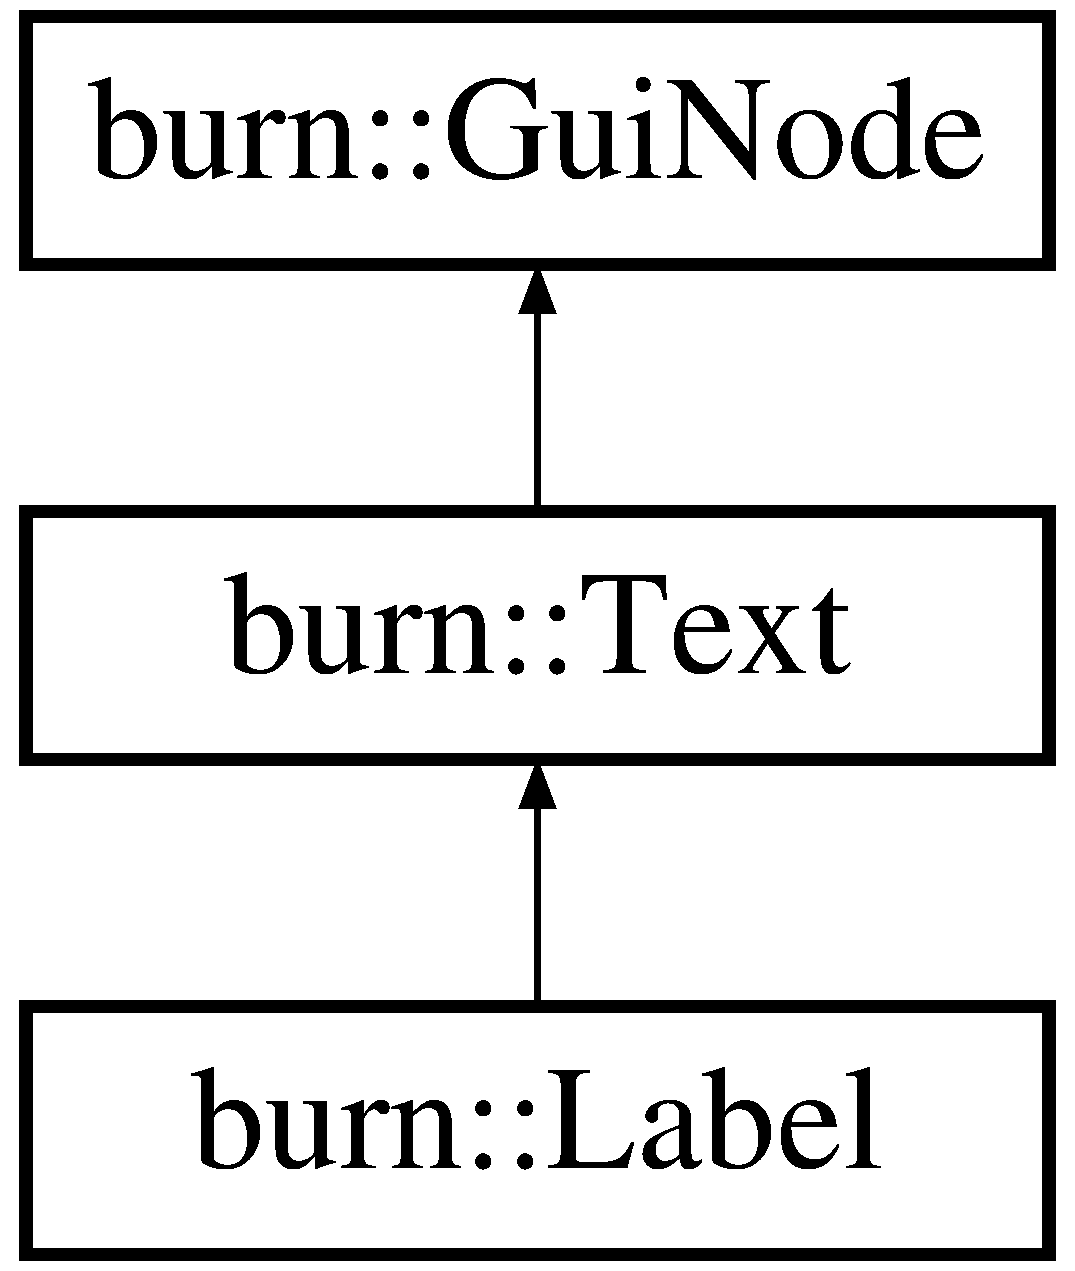
\includegraphics[height=3.000000cm]{classburn_1_1_text}
\end{center}
\end{figure}
\subsection*{Public Member Functions}
\begin{DoxyCompactItemize}
\item 
\hyperlink{classburn_1_1_text_a850dfb9cc65cd95e4eb122e586afd60d}{Text} ()
\item 
\hyperlink{classburn_1_1_text_a338a512826f16d195b37497b14ee8c9d}{$\sim$\-Text} ()
\item 
void \hyperlink{classburn_1_1_text_a414c643bde94ee0b6d339cc05470a7ba}{set\-Font\-Size} (const \hyperlink{namespaceburn_ab40b09022209bd449d317c1f0e95356b}{Uint32} \&size)
\item 
const \hyperlink{namespaceburn_ab40b09022209bd449d317c1f0e95356b}{Uint32} \& \hyperlink{classburn_1_1_text_afee8bfc930dd7f813404417f19ee2bc1}{get\-Font\-Size} () const 
\item 
void \hyperlink{classburn_1_1_text_a0b9e68d8c6e65280cccbc0372b390e7c}{set\-Text} (const \hyperlink{classburn_1_1_string}{String} \&text)
\item 
const \hyperlink{classburn_1_1_string}{String} \& \hyperlink{classburn_1_1_text_aa0892c4d1c006839d48d755b8a2951bf}{get\-Text} () const 
\item 
virtual void \hyperlink{classburn_1_1_text_aa451ad17d21dc9c12cef712aa41914bf}{draw} ()
\item 
void \hyperlink{classburn_1_1_text_ab69a87d3df7f792c48c9b13098f14b9f}{set\-Font} (const \hyperlink{classburn_1_1_font}{Font} \&font)
\item 
const \hyperlink{classburn_1_1_font}{Font} \& \hyperlink{classburn_1_1_text_a26799e9b7eacd0de8cf8f26dd6e8117a}{get\-Font} () const 
\item 
void \hyperlink{classburn_1_1_text_a1319c5bf34b0f26c7a1d341e949c5a9d}{set\-Color} (const \hyperlink{namespaceburn_a58a411b9d83c7970518a9250c1c78068}{Vector4f} \&color)
\item 
const \hyperlink{namespaceburn_a58a411b9d83c7970518a9250c1c78068}{Vector4f} \& \hyperlink{classburn_1_1_text_af5eb3305970021ae9cad3a3ca13e6e84}{get\-Color} () const 
\end{DoxyCompactItemize}
\subsection*{Protected Member Functions}
\begin{DoxyCompactItemize}
\item 
void \hyperlink{classburn_1_1_text_a5149c6fa3d5b376041d8976ae947fbf4}{draw\-String} ()
\begin{DoxyCompactList}\small\item\em Extra function for drawing the text. Used by other classes like \hyperlink{classburn_1_1_label}{Label}, that inherit from \hyperlink{classburn_1_1_text}{Text}. \end{DoxyCompactList}\end{DoxyCompactItemize}
\subsection*{Protected Attributes}
\begin{DoxyCompactItemize}
\item 
\hyperlink{classburn_1_1_string}{String} \hyperlink{classburn_1_1_text_a4d977a13462cae85ecde89f87dc73131}{\-\_\-text}
\item 
\hyperlink{classburn_1_1_font}{Font} \hyperlink{classburn_1_1_text_aae8c3744db42bcc969aef7022b5e964e}{\-\_\-font}
\item 
\hyperlink{namespaceburn_ab40b09022209bd449d317c1f0e95356b}{Uint32} \hyperlink{classburn_1_1_text_a48512684eaf0d543b8089b359b87b88f}{\-\_\-font\-Size}
\end{DoxyCompactItemize}


\subsection{Constructor \& Destructor Documentation}
\hypertarget{classburn_1_1_text_a850dfb9cc65cd95e4eb122e586afd60d}{\index{burn\-::\-Text@{burn\-::\-Text}!Text@{Text}}
\index{Text@{Text}!burn::Text@{burn\-::\-Text}}
\subsubsection[{Text}]{\setlength{\rightskip}{0pt plus 5cm}burn\-::\-Text\-::\-Text (
\begin{DoxyParamCaption}
{}
\end{DoxyParamCaption}
)}}\label{classburn_1_1_text_a850dfb9cc65cd95e4eb122e586afd60d}
\hypertarget{classburn_1_1_text_a338a512826f16d195b37497b14ee8c9d}{\index{burn\-::\-Text@{burn\-::\-Text}!$\sim$\-Text@{$\sim$\-Text}}
\index{$\sim$\-Text@{$\sim$\-Text}!burn::Text@{burn\-::\-Text}}
\subsubsection[{$\sim$\-Text}]{\setlength{\rightskip}{0pt plus 5cm}burn\-::\-Text\-::$\sim$\-Text (
\begin{DoxyParamCaption}
{}
\end{DoxyParamCaption}
)}}\label{classburn_1_1_text_a338a512826f16d195b37497b14ee8c9d}


\subsection{Member Function Documentation}
\hypertarget{classburn_1_1_text_aa451ad17d21dc9c12cef712aa41914bf}{\index{burn\-::\-Text@{burn\-::\-Text}!draw@{draw}}
\index{draw@{draw}!burn::Text@{burn\-::\-Text}}
\subsubsection[{draw}]{\setlength{\rightskip}{0pt plus 5cm}virtual void burn\-::\-Text\-::draw (
\begin{DoxyParamCaption}
{}
\end{DoxyParamCaption}
)\hspace{0.3cm}{\ttfamily [virtual]}}}\label{classburn_1_1_text_aa451ad17d21dc9c12cef712aa41914bf}


Implements \hyperlink{classburn_1_1_gui_node_ac283552733ae59c4f1b7fa05c79cb517}{burn\-::\-Gui\-Node}.



Reimplemented in \hyperlink{classburn_1_1_label_a23eaa7ccb0a68e6691a89133cb4254d5}{burn\-::\-Label}.

\hypertarget{classburn_1_1_text_a5149c6fa3d5b376041d8976ae947fbf4}{\index{burn\-::\-Text@{burn\-::\-Text}!draw\-String@{draw\-String}}
\index{draw\-String@{draw\-String}!burn::Text@{burn\-::\-Text}}
\subsubsection[{draw\-String}]{\setlength{\rightskip}{0pt plus 5cm}void burn\-::\-Text\-::draw\-String (
\begin{DoxyParamCaption}
{}
\end{DoxyParamCaption}
)\hspace{0.3cm}{\ttfamily [protected]}}}\label{classburn_1_1_text_a5149c6fa3d5b376041d8976ae947fbf4}


Extra function for drawing the text. Used by other classes like \hyperlink{classburn_1_1_label}{Label}, that inherit from \hyperlink{classburn_1_1_text}{Text}. 

\hypertarget{classburn_1_1_text_af5eb3305970021ae9cad3a3ca13e6e84}{\index{burn\-::\-Text@{burn\-::\-Text}!get\-Color@{get\-Color}}
\index{get\-Color@{get\-Color}!burn::Text@{burn\-::\-Text}}
\subsubsection[{get\-Color}]{\setlength{\rightskip}{0pt plus 5cm}const {\bf Vector4f}\& burn\-::\-Text\-::get\-Color (
\begin{DoxyParamCaption}
{}
\end{DoxyParamCaption}
) const}}\label{classburn_1_1_text_af5eb3305970021ae9cad3a3ca13e6e84}
\hypertarget{classburn_1_1_text_a26799e9b7eacd0de8cf8f26dd6e8117a}{\index{burn\-::\-Text@{burn\-::\-Text}!get\-Font@{get\-Font}}
\index{get\-Font@{get\-Font}!burn::Text@{burn\-::\-Text}}
\subsubsection[{get\-Font}]{\setlength{\rightskip}{0pt plus 5cm}const {\bf Font}\& burn\-::\-Text\-::get\-Font (
\begin{DoxyParamCaption}
{}
\end{DoxyParamCaption}
) const}}\label{classburn_1_1_text_a26799e9b7eacd0de8cf8f26dd6e8117a}
\hypertarget{classburn_1_1_text_afee8bfc930dd7f813404417f19ee2bc1}{\index{burn\-::\-Text@{burn\-::\-Text}!get\-Font\-Size@{get\-Font\-Size}}
\index{get\-Font\-Size@{get\-Font\-Size}!burn::Text@{burn\-::\-Text}}
\subsubsection[{get\-Font\-Size}]{\setlength{\rightskip}{0pt plus 5cm}const {\bf Uint32}\& burn\-::\-Text\-::get\-Font\-Size (
\begin{DoxyParamCaption}
{}
\end{DoxyParamCaption}
) const}}\label{classburn_1_1_text_afee8bfc930dd7f813404417f19ee2bc1}
\hypertarget{classburn_1_1_text_aa0892c4d1c006839d48d755b8a2951bf}{\index{burn\-::\-Text@{burn\-::\-Text}!get\-Text@{get\-Text}}
\index{get\-Text@{get\-Text}!burn::Text@{burn\-::\-Text}}
\subsubsection[{get\-Text}]{\setlength{\rightskip}{0pt plus 5cm}const {\bf String}\& burn\-::\-Text\-::get\-Text (
\begin{DoxyParamCaption}
{}
\end{DoxyParamCaption}
) const}}\label{classburn_1_1_text_aa0892c4d1c006839d48d755b8a2951bf}
\hypertarget{classburn_1_1_text_a1319c5bf34b0f26c7a1d341e949c5a9d}{\index{burn\-::\-Text@{burn\-::\-Text}!set\-Color@{set\-Color}}
\index{set\-Color@{set\-Color}!burn::Text@{burn\-::\-Text}}
\subsubsection[{set\-Color}]{\setlength{\rightskip}{0pt plus 5cm}void burn\-::\-Text\-::set\-Color (
\begin{DoxyParamCaption}
\item[{const {\bf Vector4f} \&}]{color}
\end{DoxyParamCaption}
)}}\label{classburn_1_1_text_a1319c5bf34b0f26c7a1d341e949c5a9d}
\hypertarget{classburn_1_1_text_ab69a87d3df7f792c48c9b13098f14b9f}{\index{burn\-::\-Text@{burn\-::\-Text}!set\-Font@{set\-Font}}
\index{set\-Font@{set\-Font}!burn::Text@{burn\-::\-Text}}
\subsubsection[{set\-Font}]{\setlength{\rightskip}{0pt plus 5cm}void burn\-::\-Text\-::set\-Font (
\begin{DoxyParamCaption}
\item[{const {\bf Font} \&}]{font}
\end{DoxyParamCaption}
)}}\label{classburn_1_1_text_ab69a87d3df7f792c48c9b13098f14b9f}
\hypertarget{classburn_1_1_text_a414c643bde94ee0b6d339cc05470a7ba}{\index{burn\-::\-Text@{burn\-::\-Text}!set\-Font\-Size@{set\-Font\-Size}}
\index{set\-Font\-Size@{set\-Font\-Size}!burn::Text@{burn\-::\-Text}}
\subsubsection[{set\-Font\-Size}]{\setlength{\rightskip}{0pt plus 5cm}void burn\-::\-Text\-::set\-Font\-Size (
\begin{DoxyParamCaption}
\item[{const {\bf Uint32} \&}]{size}
\end{DoxyParamCaption}
)}}\label{classburn_1_1_text_a414c643bde94ee0b6d339cc05470a7ba}
\hypertarget{classburn_1_1_text_a0b9e68d8c6e65280cccbc0372b390e7c}{\index{burn\-::\-Text@{burn\-::\-Text}!set\-Text@{set\-Text}}
\index{set\-Text@{set\-Text}!burn::Text@{burn\-::\-Text}}
\subsubsection[{set\-Text}]{\setlength{\rightskip}{0pt plus 5cm}void burn\-::\-Text\-::set\-Text (
\begin{DoxyParamCaption}
\item[{const {\bf String} \&}]{text}
\end{DoxyParamCaption}
)}}\label{classburn_1_1_text_a0b9e68d8c6e65280cccbc0372b390e7c}


\subsection{Member Data Documentation}
\hypertarget{classburn_1_1_text_aae8c3744db42bcc969aef7022b5e964e}{\index{burn\-::\-Text@{burn\-::\-Text}!\-\_\-font@{\-\_\-font}}
\index{\-\_\-font@{\-\_\-font}!burn::Text@{burn\-::\-Text}}
\subsubsection[{\-\_\-font}]{\setlength{\rightskip}{0pt plus 5cm}{\bf Font} burn\-::\-Text\-::\-\_\-font\hspace{0.3cm}{\ttfamily [protected]}}}\label{classburn_1_1_text_aae8c3744db42bcc969aef7022b5e964e}
\hypertarget{classburn_1_1_text_a48512684eaf0d543b8089b359b87b88f}{\index{burn\-::\-Text@{burn\-::\-Text}!\-\_\-font\-Size@{\-\_\-font\-Size}}
\index{\-\_\-font\-Size@{\-\_\-font\-Size}!burn::Text@{burn\-::\-Text}}
\subsubsection[{\-\_\-font\-Size}]{\setlength{\rightskip}{0pt plus 5cm}{\bf Uint32} burn\-::\-Text\-::\-\_\-font\-Size\hspace{0.3cm}{\ttfamily [protected]}}}\label{classburn_1_1_text_a48512684eaf0d543b8089b359b87b88f}
\hypertarget{classburn_1_1_text_a4d977a13462cae85ecde89f87dc73131}{\index{burn\-::\-Text@{burn\-::\-Text}!\-\_\-text@{\-\_\-text}}
\index{\-\_\-text@{\-\_\-text}!burn::Text@{burn\-::\-Text}}
\subsubsection[{\-\_\-text}]{\setlength{\rightskip}{0pt plus 5cm}{\bf String} burn\-::\-Text\-::\-\_\-text\hspace{0.3cm}{\ttfamily [protected]}}}\label{classburn_1_1_text_a4d977a13462cae85ecde89f87dc73131}


The documentation for this class was generated from the following file\-:\begin{DoxyCompactItemize}
\item 
include/\-Burngine/\-Graphics/\-Gui/\hyperlink{_text_8h}{Text.\-h}\end{DoxyCompactItemize}

\hypertarget{classburn_1_1_texture}{\section{burn\-:\-:Texture Class Reference}
\label{classburn_1_1_texture}\index{burn\-::\-Texture@{burn\-::\-Texture}}
}


Holds Open\-G\-L comfort images as textures.  




{\ttfamily \#include $<$Texture.\-h$>$}

Inheritance diagram for burn\-:\-:Texture\-:\begin{figure}[H]
\begin{center}
\leavevmode
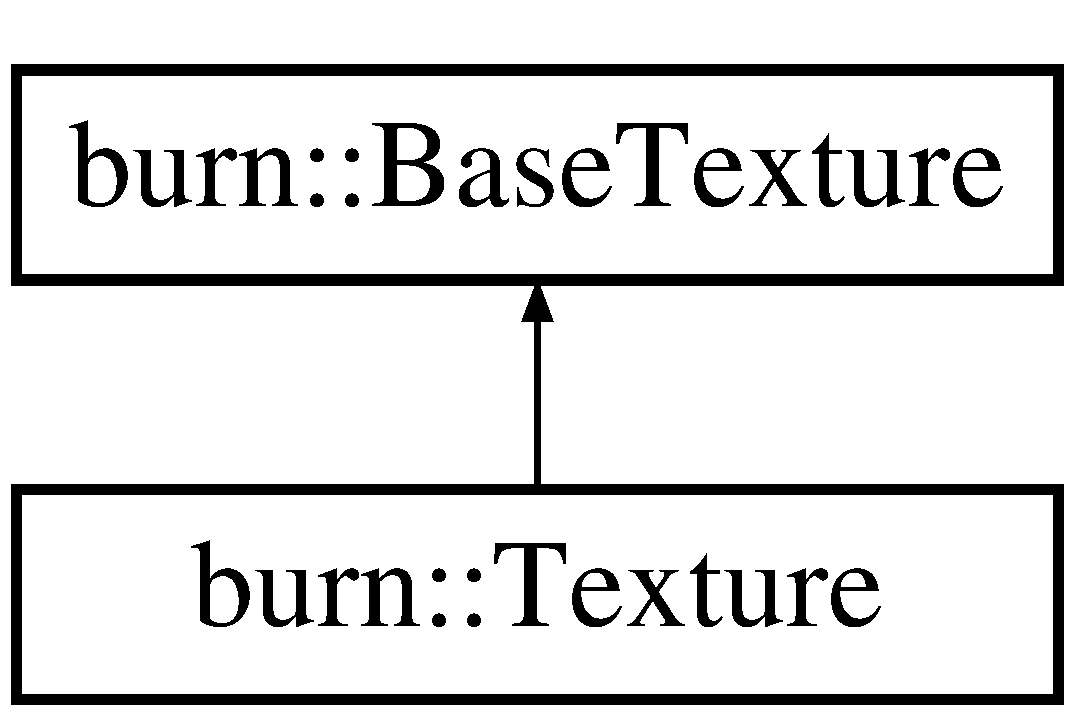
\includegraphics[height=2.000000cm]{classburn_1_1_texture}
\end{center}
\end{figure}
\subsection*{Public Member Functions}
\begin{DoxyCompactItemize}
\item 
\hyperlink{classburn_1_1_texture_ac44cabdfa800d3881a78e9bfa6a90a77}{Texture} ()
\item 
\hyperlink{classburn_1_1_texture_a8878f6109bcbfdc3171516f43ed7c3c6}{Texture} (const \hyperlink{classburn_1_1_texture}{Texture} \&other)
\item 
\hyperlink{classburn_1_1_texture}{Texture} \& \hyperlink{classburn_1_1_texture_a54465cf7f59f204405b3ea7e110686af}{operator=} (const \hyperlink{classburn_1_1_texture}{Texture} \&other)
\item 
\hyperlink{classburn_1_1_texture_a2652ca0b245b24ef802bb20a99d8248f}{$\sim$\-Texture} ()
\item 
bool \hyperlink{classburn_1_1_texture_a96d10626c422ea8dbc2cd51105061128}{load\-From\-File} (const std\-::string \&file)
\begin{DoxyCompactList}\small\item\em Loads an image from file and stores it as texture ready for use. \end{DoxyCompactList}\item 
bool \hyperlink{classburn_1_1_texture_a5b0db64283a0b8fb24f332e461019893}{load\-From\-Data} (G\-Lubyte $\ast$data, const \hyperlink{namespaceburn_a6805fa33c49c4c3db88a7bebba2c408f}{Vector2ui} \&dimensions, const \hyperlink{namespaceburn_a96c2e82d6da686c64a6f330628466b05}{Int32} \&bpp, const G\-Lenum \&format)
\end{DoxyCompactItemize}
\subsection*{Protected Member Functions}
\begin{DoxyCompactItemize}
\item 
virtual void \hyperlink{classburn_1_1_texture_a41cf19a71e61bb8ddfd6bf93d1c0ef02}{on\-Bind} (const unsigned int \&unit) const 
\item 
virtual void \hyperlink{classburn_1_1_texture_a1a2a5e886e044ac83fa575916129884f}{on\-Unbind} (const unsigned int \&unit) const 
\end{DoxyCompactItemize}
\subsection*{Protected Attributes}
\begin{DoxyCompactItemize}
\item 
G\-Luint \hyperlink{classburn_1_1_texture_a03d6a7665e62581007271195df866aaa}{\-\_\-texture\-Id}
\end{DoxyCompactItemize}
\subsection*{Additional Inherited Members}


\subsection{Detailed Description}
Holds Open\-G\-L comfort images as textures. 

\subsection{Constructor \& Destructor Documentation}
\hypertarget{classburn_1_1_texture_ac44cabdfa800d3881a78e9bfa6a90a77}{\index{burn\-::\-Texture@{burn\-::\-Texture}!Texture@{Texture}}
\index{Texture@{Texture}!burn::Texture@{burn\-::\-Texture}}
\subsubsection[{Texture}]{\setlength{\rightskip}{0pt plus 5cm}burn\-::\-Texture\-::\-Texture (
\begin{DoxyParamCaption}
{}
\end{DoxyParamCaption}
)}}\label{classburn_1_1_texture_ac44cabdfa800d3881a78e9bfa6a90a77}
\hypertarget{classburn_1_1_texture_a8878f6109bcbfdc3171516f43ed7c3c6}{\index{burn\-::\-Texture@{burn\-::\-Texture}!Texture@{Texture}}
\index{Texture@{Texture}!burn::Texture@{burn\-::\-Texture}}
\subsubsection[{Texture}]{\setlength{\rightskip}{0pt plus 5cm}burn\-::\-Texture\-::\-Texture (
\begin{DoxyParamCaption}
\item[{const {\bf Texture} \&}]{other}
\end{DoxyParamCaption}
)}}\label{classburn_1_1_texture_a8878f6109bcbfdc3171516f43ed7c3c6}
\hypertarget{classburn_1_1_texture_a2652ca0b245b24ef802bb20a99d8248f}{\index{burn\-::\-Texture@{burn\-::\-Texture}!$\sim$\-Texture@{$\sim$\-Texture}}
\index{$\sim$\-Texture@{$\sim$\-Texture}!burn::Texture@{burn\-::\-Texture}}
\subsubsection[{$\sim$\-Texture}]{\setlength{\rightskip}{0pt plus 5cm}burn\-::\-Texture\-::$\sim$\-Texture (
\begin{DoxyParamCaption}
{}
\end{DoxyParamCaption}
)}}\label{classburn_1_1_texture_a2652ca0b245b24ef802bb20a99d8248f}


\subsection{Member Function Documentation}
\hypertarget{classburn_1_1_texture_a5b0db64283a0b8fb24f332e461019893}{\index{burn\-::\-Texture@{burn\-::\-Texture}!load\-From\-Data@{load\-From\-Data}}
\index{load\-From\-Data@{load\-From\-Data}!burn::Texture@{burn\-::\-Texture}}
\subsubsection[{load\-From\-Data}]{\setlength{\rightskip}{0pt plus 5cm}bool burn\-::\-Texture\-::load\-From\-Data (
\begin{DoxyParamCaption}
\item[{G\-Lubyte $\ast$}]{data, }
\item[{const {\bf Vector2ui} \&}]{dimensions, }
\item[{const {\bf Int32} \&}]{bpp, }
\item[{const G\-Lenum \&}]{format}
\end{DoxyParamCaption}
)}}\label{classburn_1_1_texture_a5b0db64283a0b8fb24f332e461019893}
\hypertarget{classburn_1_1_texture_a96d10626c422ea8dbc2cd51105061128}{\index{burn\-::\-Texture@{burn\-::\-Texture}!load\-From\-File@{load\-From\-File}}
\index{load\-From\-File@{load\-From\-File}!burn::Texture@{burn\-::\-Texture}}
\subsubsection[{load\-From\-File}]{\setlength{\rightskip}{0pt plus 5cm}bool burn\-::\-Texture\-::load\-From\-File (
\begin{DoxyParamCaption}
\item[{const std\-::string \&}]{file}
\end{DoxyParamCaption}
)}}\label{classburn_1_1_texture_a96d10626c422ea8dbc2cd51105061128}


Loads an image from file and stores it as texture ready for use. 


\begin{DoxyParams}{Parameters}
{\em file} & The image to load\\
\hline
\end{DoxyParams}
\begin{DoxyReturn}{Returns}
Returns true on success 
\end{DoxyReturn}
\hypertarget{classburn_1_1_texture_a41cf19a71e61bb8ddfd6bf93d1c0ef02}{\index{burn\-::\-Texture@{burn\-::\-Texture}!on\-Bind@{on\-Bind}}
\index{on\-Bind@{on\-Bind}!burn::Texture@{burn\-::\-Texture}}
\subsubsection[{on\-Bind}]{\setlength{\rightskip}{0pt plus 5cm}virtual void burn\-::\-Texture\-::on\-Bind (
\begin{DoxyParamCaption}
\item[{const unsigned int \&}]{unit}
\end{DoxyParamCaption}
) const\hspace{0.3cm}{\ttfamily [protected]}, {\ttfamily [virtual]}}}\label{classburn_1_1_texture_a41cf19a71e61bb8ddfd6bf93d1c0ef02}


Implements \hyperlink{classburn_1_1_base_texture_a1102bd72393ccc77bd1fc47e046b4900}{burn\-::\-Base\-Texture}.

\hypertarget{classburn_1_1_texture_a1a2a5e886e044ac83fa575916129884f}{\index{burn\-::\-Texture@{burn\-::\-Texture}!on\-Unbind@{on\-Unbind}}
\index{on\-Unbind@{on\-Unbind}!burn::Texture@{burn\-::\-Texture}}
\subsubsection[{on\-Unbind}]{\setlength{\rightskip}{0pt plus 5cm}virtual void burn\-::\-Texture\-::on\-Unbind (
\begin{DoxyParamCaption}
\item[{const unsigned int \&}]{unit}
\end{DoxyParamCaption}
) const\hspace{0.3cm}{\ttfamily [protected]}, {\ttfamily [virtual]}}}\label{classburn_1_1_texture_a1a2a5e886e044ac83fa575916129884f}


Implements \hyperlink{classburn_1_1_base_texture_a06c69280f4bed1ac923cfeacad6a2aa6}{burn\-::\-Base\-Texture}.

\hypertarget{classburn_1_1_texture_a54465cf7f59f204405b3ea7e110686af}{\index{burn\-::\-Texture@{burn\-::\-Texture}!operator=@{operator=}}
\index{operator=@{operator=}!burn::Texture@{burn\-::\-Texture}}
\subsubsection[{operator=}]{\setlength{\rightskip}{0pt plus 5cm}{\bf Texture}\& burn\-::\-Texture\-::operator= (
\begin{DoxyParamCaption}
\item[{const {\bf Texture} \&}]{other}
\end{DoxyParamCaption}
)}}\label{classburn_1_1_texture_a54465cf7f59f204405b3ea7e110686af}


\subsection{Member Data Documentation}
\hypertarget{classburn_1_1_texture_a03d6a7665e62581007271195df866aaa}{\index{burn\-::\-Texture@{burn\-::\-Texture}!\-\_\-texture\-Id@{\-\_\-texture\-Id}}
\index{\-\_\-texture\-Id@{\-\_\-texture\-Id}!burn::Texture@{burn\-::\-Texture}}
\subsubsection[{\-\_\-texture\-Id}]{\setlength{\rightskip}{0pt plus 5cm}G\-Luint burn\-::\-Texture\-::\-\_\-texture\-Id\hspace{0.3cm}{\ttfamily [protected]}}}\label{classburn_1_1_texture_a03d6a7665e62581007271195df866aaa}


The documentation for this class was generated from the following file\-:\begin{DoxyCompactItemize}
\item 
include/\-Burngine/\-Graphics/\-Texture/\hyperlink{_texture_8h}{Texture.\-h}\end{DoxyCompactItemize}

\hypertarget{classburn_1_1_time}{\section{burn\-:\-:Time Class Reference}
\label{classburn_1_1_time}\index{burn\-::\-Time@{burn\-::\-Time}}
}


{\ttfamily \#include $<$Time.\-h$>$}

\subsection*{Public Member Functions}
\begin{DoxyCompactItemize}
\item 
\hyperlink{classburn_1_1_time_a1d23a0a88aa2eeb342a2d8acb4b86cf3}{Time} ()
\item 
\hyperlink{classburn_1_1_time_ac56700cc46aa55773938f1f3fe1bdc4e}{Time} (const \hyperlink{namespaceburn_a431c4128e194f6d8909971ef6253bca9}{Time\-Point} \&point)
\item 
void \hyperlink{classburn_1_1_time_a360877b3779ec6fd3e4993f1fc4a48c3}{set\-Time} (const \hyperlink{namespaceburn_a431c4128e194f6d8909971ef6253bca9}{Time\-Point} \&point)
\item 
long double \hyperlink{classburn_1_1_time_a5fcb537fbce65dc08b54e6494de42fce}{as\-Seconds} () const 
\item 
unsigned long long \hyperlink{classburn_1_1_time_ad55a56bdd08f72d0649bcd54c658bb82}{as\-Milliseconds} () const 
\item 
unsigned long long \hyperlink{classburn_1_1_time_a0fb0aaabbbf1f186f91231b3d987203e}{as\-Microseconds} () const 
\item 
unsigned long long \hyperlink{classburn_1_1_time_a104120a69544ee338f93c32a6663c35a}{as\-Nanoseconds} () const 
\item 
\hyperlink{classburn_1_1_time}{Time} \hyperlink{classburn_1_1_time_a28ec8ef74d89d1ef200a41a6aa5a9ccd}{operator-\/} (const \hyperlink{classburn_1_1_time}{Time} \&other) const 
\item 
const \hyperlink{namespaceburn_a431c4128e194f6d8909971ef6253bca9}{Time\-Point} \& \hyperlink{classburn_1_1_time_a67c20bcaf4e0c38264e88e78b8e641ad}{get\-Time\-Point} () const 
\end{DoxyCompactItemize}
\subsection*{Static Public Member Functions}
\begin{DoxyCompactItemize}
\item 
static \hyperlink{namespaceburn_a431c4128e194f6d8909971ef6253bca9}{Time\-Point} \hyperlink{classburn_1_1_time_a8dea3176bee9f79b8a910ab8584fecc1}{seconds} (const double \&seconds)
\item 
static \hyperlink{namespaceburn_a431c4128e194f6d8909971ef6253bca9}{Time\-Point} \hyperlink{classburn_1_1_time_aca78c2d40cc49cf3fac16db1caf6740e}{milliseconds} (const int \&milliseconds)
\item 
static \hyperlink{namespaceburn_a431c4128e194f6d8909971ef6253bca9}{Time\-Point} \hyperlink{classburn_1_1_time_a7a07a638e213f62fff0de476ac3cb085}{now} ()
\end{DoxyCompactItemize}


\subsection{Constructor \& Destructor Documentation}
\hypertarget{classburn_1_1_time_a1d23a0a88aa2eeb342a2d8acb4b86cf3}{\index{burn\-::\-Time@{burn\-::\-Time}!Time@{Time}}
\index{Time@{Time}!burn::Time@{burn\-::\-Time}}
\subsubsection[{Time}]{\setlength{\rightskip}{0pt plus 5cm}burn\-::\-Time\-::\-Time (
\begin{DoxyParamCaption}
{}
\end{DoxyParamCaption}
)}}\label{classburn_1_1_time_a1d23a0a88aa2eeb342a2d8acb4b86cf3}
\hypertarget{classburn_1_1_time_ac56700cc46aa55773938f1f3fe1bdc4e}{\index{burn\-::\-Time@{burn\-::\-Time}!Time@{Time}}
\index{Time@{Time}!burn::Time@{burn\-::\-Time}}
\subsubsection[{Time}]{\setlength{\rightskip}{0pt plus 5cm}burn\-::\-Time\-::\-Time (
\begin{DoxyParamCaption}
\item[{const {\bf Time\-Point} \&}]{point}
\end{DoxyParamCaption}
)}}\label{classburn_1_1_time_ac56700cc46aa55773938f1f3fe1bdc4e}


\subsection{Member Function Documentation}
\hypertarget{classburn_1_1_time_a0fb0aaabbbf1f186f91231b3d987203e}{\index{burn\-::\-Time@{burn\-::\-Time}!as\-Microseconds@{as\-Microseconds}}
\index{as\-Microseconds@{as\-Microseconds}!burn::Time@{burn\-::\-Time}}
\subsubsection[{as\-Microseconds}]{\setlength{\rightskip}{0pt plus 5cm}unsigned long long burn\-::\-Time\-::as\-Microseconds (
\begin{DoxyParamCaption}
{}
\end{DoxyParamCaption}
) const}}\label{classburn_1_1_time_a0fb0aaabbbf1f186f91231b3d987203e}
\hypertarget{classburn_1_1_time_ad55a56bdd08f72d0649bcd54c658bb82}{\index{burn\-::\-Time@{burn\-::\-Time}!as\-Milliseconds@{as\-Milliseconds}}
\index{as\-Milliseconds@{as\-Milliseconds}!burn::Time@{burn\-::\-Time}}
\subsubsection[{as\-Milliseconds}]{\setlength{\rightskip}{0pt plus 5cm}unsigned long long burn\-::\-Time\-::as\-Milliseconds (
\begin{DoxyParamCaption}
{}
\end{DoxyParamCaption}
) const}}\label{classburn_1_1_time_ad55a56bdd08f72d0649bcd54c658bb82}
\hypertarget{classburn_1_1_time_a104120a69544ee338f93c32a6663c35a}{\index{burn\-::\-Time@{burn\-::\-Time}!as\-Nanoseconds@{as\-Nanoseconds}}
\index{as\-Nanoseconds@{as\-Nanoseconds}!burn::Time@{burn\-::\-Time}}
\subsubsection[{as\-Nanoseconds}]{\setlength{\rightskip}{0pt plus 5cm}unsigned long long burn\-::\-Time\-::as\-Nanoseconds (
\begin{DoxyParamCaption}
{}
\end{DoxyParamCaption}
) const}}\label{classburn_1_1_time_a104120a69544ee338f93c32a6663c35a}
\hypertarget{classburn_1_1_time_a5fcb537fbce65dc08b54e6494de42fce}{\index{burn\-::\-Time@{burn\-::\-Time}!as\-Seconds@{as\-Seconds}}
\index{as\-Seconds@{as\-Seconds}!burn::Time@{burn\-::\-Time}}
\subsubsection[{as\-Seconds}]{\setlength{\rightskip}{0pt plus 5cm}long double burn\-::\-Time\-::as\-Seconds (
\begin{DoxyParamCaption}
{}
\end{DoxyParamCaption}
) const}}\label{classburn_1_1_time_a5fcb537fbce65dc08b54e6494de42fce}
\hypertarget{classburn_1_1_time_a67c20bcaf4e0c38264e88e78b8e641ad}{\index{burn\-::\-Time@{burn\-::\-Time}!get\-Time\-Point@{get\-Time\-Point}}
\index{get\-Time\-Point@{get\-Time\-Point}!burn::Time@{burn\-::\-Time}}
\subsubsection[{get\-Time\-Point}]{\setlength{\rightskip}{0pt plus 5cm}const {\bf Time\-Point}\& burn\-::\-Time\-::get\-Time\-Point (
\begin{DoxyParamCaption}
{}
\end{DoxyParamCaption}
) const}}\label{classburn_1_1_time_a67c20bcaf4e0c38264e88e78b8e641ad}
\hypertarget{classburn_1_1_time_aca78c2d40cc49cf3fac16db1caf6740e}{\index{burn\-::\-Time@{burn\-::\-Time}!milliseconds@{milliseconds}}
\index{milliseconds@{milliseconds}!burn::Time@{burn\-::\-Time}}
\subsubsection[{milliseconds}]{\setlength{\rightskip}{0pt plus 5cm}static {\bf Time\-Point} burn\-::\-Time\-::milliseconds (
\begin{DoxyParamCaption}
\item[{const int \&}]{milliseconds}
\end{DoxyParamCaption}
)\hspace{0.3cm}{\ttfamily [static]}}}\label{classburn_1_1_time_aca78c2d40cc49cf3fac16db1caf6740e}
\hypertarget{classburn_1_1_time_a7a07a638e213f62fff0de476ac3cb085}{\index{burn\-::\-Time@{burn\-::\-Time}!now@{now}}
\index{now@{now}!burn::Time@{burn\-::\-Time}}
\subsubsection[{now}]{\setlength{\rightskip}{0pt plus 5cm}static {\bf Time\-Point} burn\-::\-Time\-::now (
\begin{DoxyParamCaption}
{}
\end{DoxyParamCaption}
)\hspace{0.3cm}{\ttfamily [static]}}}\label{classburn_1_1_time_a7a07a638e213f62fff0de476ac3cb085}
\hypertarget{classburn_1_1_time_a28ec8ef74d89d1ef200a41a6aa5a9ccd}{\index{burn\-::\-Time@{burn\-::\-Time}!operator-\/@{operator-\/}}
\index{operator-\/@{operator-\/}!burn::Time@{burn\-::\-Time}}
\subsubsection[{operator-\/}]{\setlength{\rightskip}{0pt plus 5cm}{\bf Time} burn\-::\-Time\-::operator-\/ (
\begin{DoxyParamCaption}
\item[{const {\bf Time} \&}]{other}
\end{DoxyParamCaption}
) const}}\label{classburn_1_1_time_a28ec8ef74d89d1ef200a41a6aa5a9ccd}
\hypertarget{classburn_1_1_time_a8dea3176bee9f79b8a910ab8584fecc1}{\index{burn\-::\-Time@{burn\-::\-Time}!seconds@{seconds}}
\index{seconds@{seconds}!burn::Time@{burn\-::\-Time}}
\subsubsection[{seconds}]{\setlength{\rightskip}{0pt plus 5cm}static {\bf Time\-Point} burn\-::\-Time\-::seconds (
\begin{DoxyParamCaption}
\item[{const double \&}]{seconds}
\end{DoxyParamCaption}
)\hspace{0.3cm}{\ttfamily [static]}}}\label{classburn_1_1_time_a8dea3176bee9f79b8a910ab8584fecc1}
\hypertarget{classburn_1_1_time_a360877b3779ec6fd3e4993f1fc4a48c3}{\index{burn\-::\-Time@{burn\-::\-Time}!set\-Time@{set\-Time}}
\index{set\-Time@{set\-Time}!burn::Time@{burn\-::\-Time}}
\subsubsection[{set\-Time}]{\setlength{\rightskip}{0pt plus 5cm}void burn\-::\-Time\-::set\-Time (
\begin{DoxyParamCaption}
\item[{const {\bf Time\-Point} \&}]{point}
\end{DoxyParamCaption}
)}}\label{classburn_1_1_time_a360877b3779ec6fd3e4993f1fc4a48c3}


The documentation for this class was generated from the following file\-:\begin{DoxyCompactItemize}
\item 
include/\-Burngine/\-System/\hyperlink{_time_8h}{Time.\-h}\end{DoxyCompactItemize}

\hypertarget{classburn_1_1_transformable}{\section{burn\-:\-:Transformable Class Reference}
\label{classburn_1_1_transformable}\index{burn\-::\-Transformable@{burn\-::\-Transformable}}
}


Provides methods to move an object in 3\-D-\/space.  




{\ttfamily \#include $<$Transformable.\-h$>$}

Inheritance diagram for burn\-:\-:Transformable\-:\begin{figure}[H]
\begin{center}
\leavevmode
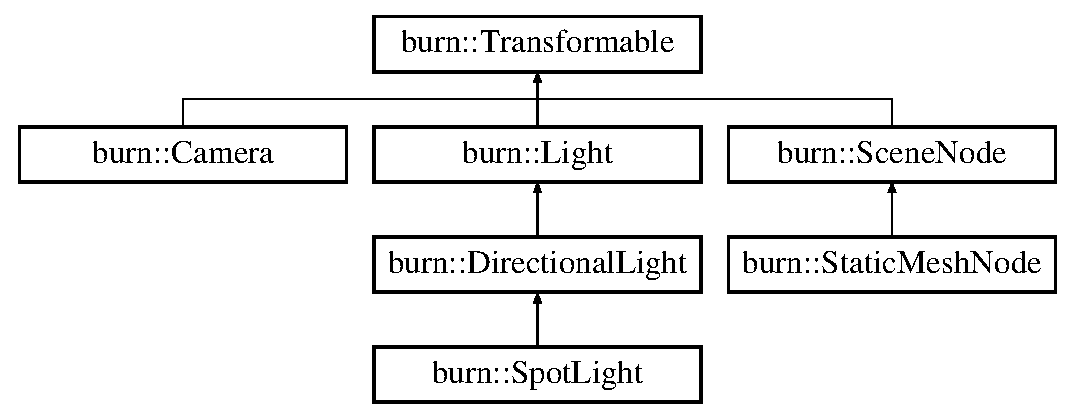
\includegraphics[height=4.000000cm]{classburn_1_1_transformable}
\end{center}
\end{figure}
\subsection*{Public Member Functions}
\begin{DoxyCompactItemize}
\item 
\hyperlink{classburn_1_1_transformable_ab5df8f6f319ebc8888465632a1567981}{Transformable} ()
\begin{DoxyCompactList}\small\item\em The default constructor. \end{DoxyCompactList}\item 
\hyperlink{classburn_1_1_transformable_a96fb19be22efcefb4723781146de28fe}{Transformable} (const \hyperlink{classburn_1_1_transformable}{Transformable} \&other)
\item 
\hyperlink{classburn_1_1_transformable}{Transformable} \& \hyperlink{classburn_1_1_transformable_aee23249ee60e4a3e590046e633c3a979}{operator=} (const \hyperlink{classburn_1_1_transformable}{Transformable} \&other)
\item 
virtual \hyperlink{classburn_1_1_transformable_ac3b6e91f17a6b8f5db8027e72942f269}{$\sim$\-Transformable} ()
\begin{DoxyCompactList}\small\item\em Virtual destructor, because this class should be derived only. \end{DoxyCompactList}\item 
void \hyperlink{classburn_1_1_transformable_a408d484d0ed48c1d7499391b3f2d4a66}{set\-Position} (const \hyperlink{namespaceburn_afdd7cfb352b9612432faf6947b6fff74}{Vector3f} \&position)
\begin{DoxyCompactList}\small\item\em Sets the position of the object. \end{DoxyCompactList}\item 
const \hyperlink{namespaceburn_afdd7cfb352b9612432faf6947b6fff74}{Vector3f} \& \hyperlink{classburn_1_1_transformable_aab2eb6fb8e64349a9f83bc6939477b74}{get\-Position} () const 
\begin{DoxyCompactList}\small\item\em Returns the current position of the object. \end{DoxyCompactList}\item 
void \hyperlink{classburn_1_1_transformable_adad877d654e3ac20ed0ff6edf002e040}{set\-Rotation} (const \hyperlink{namespaceburn_afdd7cfb352b9612432faf6947b6fff74}{Vector3f} \&rotation)
\begin{DoxyCompactList}\small\item\em Sets the rotation of the object. \end{DoxyCompactList}\item 
const \hyperlink{namespaceburn_afdd7cfb352b9612432faf6947b6fff74}{Vector3f} \& \hyperlink{classburn_1_1_transformable_af16b32fb2143e7a459b8446e898c4359}{get\-Rotation} () const 
\begin{DoxyCompactList}\small\item\em Returns the current rotation of the object. \end{DoxyCompactList}\item 
void \hyperlink{classburn_1_1_transformable_a7e73a5706524923d4fc6c13990b7f575}{set\-Scale} (const \hyperlink{namespaceburn_afdd7cfb352b9612432faf6947b6fff74}{Vector3f} \&scale)
\begin{DoxyCompactList}\small\item\em Sets the scale of the object. \end{DoxyCompactList}\item 
const \hyperlink{namespaceburn_afdd7cfb352b9612432faf6947b6fff74}{Vector3f} \& \hyperlink{classburn_1_1_transformable_a62d533b4a7d03b3b2aa9c783cb7cb061}{get\-Scale} () const 
\begin{DoxyCompactList}\small\item\em Return the current scale of the object. \end{DoxyCompactList}\item 
const \hyperlink{namespaceburn_a643e9d2ffceb4304e3755a100268a7a3}{Matrix4f} \& \hyperlink{classburn_1_1_transformable_ac77cb89c24baf4eaf730b478b2f9b2b5}{get\-Model\-Matrix} ()
\begin{DoxyCompactList}\small\item\em Returns the current modelmatrix of the object. \end{DoxyCompactList}\end{DoxyCompactItemize}
\subsection*{Protected Attributes}
\begin{DoxyCompactItemize}
\item 
\hyperlink{namespaceburn_afdd7cfb352b9612432faf6947b6fff74}{Vector3f} \hyperlink{classburn_1_1_transformable_a1cb1a52f8518c7c2f50e45d8cd902767}{\-\_\-position}
\item 
\hyperlink{namespaceburn_afdd7cfb352b9612432faf6947b6fff74}{Vector3f} \hyperlink{classburn_1_1_transformable_a80e5ca4d02b2d58593b751b040e86492}{\-\_\-scale}
\item 
\hyperlink{namespaceburn_afdd7cfb352b9612432faf6947b6fff74}{Vector3f} \hyperlink{classburn_1_1_transformable_ad62e417f44d78cbeedfd30e62c1b896d}{\-\_\-rotation}
\item 
\hyperlink{namespaceburn_a643e9d2ffceb4304e3755a100268a7a3}{Matrix4f} \hyperlink{classburn_1_1_transformable_a6a06bcec86a7f2e70eba6fe7e8bbe61c}{\-\_\-model\-Matrix}
\end{DoxyCompactItemize}


\subsection{Detailed Description}
Provides methods to move an object in 3\-D-\/space. 

\subsection{Constructor \& Destructor Documentation}
\hypertarget{classburn_1_1_transformable_ab5df8f6f319ebc8888465632a1567981}{\index{burn\-::\-Transformable@{burn\-::\-Transformable}!Transformable@{Transformable}}
\index{Transformable@{Transformable}!burn::Transformable@{burn\-::\-Transformable}}
\subsubsection[{Transformable}]{\setlength{\rightskip}{0pt plus 5cm}burn\-::\-Transformable\-::\-Transformable (
\begin{DoxyParamCaption}
{}
\end{DoxyParamCaption}
)}}\label{classburn_1_1_transformable_ab5df8f6f319ebc8888465632a1567981}


The default constructor. 

\hypertarget{classburn_1_1_transformable_a96fb19be22efcefb4723781146de28fe}{\index{burn\-::\-Transformable@{burn\-::\-Transformable}!Transformable@{Transformable}}
\index{Transformable@{Transformable}!burn::Transformable@{burn\-::\-Transformable}}
\subsubsection[{Transformable}]{\setlength{\rightskip}{0pt plus 5cm}burn\-::\-Transformable\-::\-Transformable (
\begin{DoxyParamCaption}
\item[{const {\bf Transformable} \&}]{other}
\end{DoxyParamCaption}
)}}\label{classburn_1_1_transformable_a96fb19be22efcefb4723781146de28fe}
\hypertarget{classburn_1_1_transformable_ac3b6e91f17a6b8f5db8027e72942f269}{\index{burn\-::\-Transformable@{burn\-::\-Transformable}!$\sim$\-Transformable@{$\sim$\-Transformable}}
\index{$\sim$\-Transformable@{$\sim$\-Transformable}!burn::Transformable@{burn\-::\-Transformable}}
\subsubsection[{$\sim$\-Transformable}]{\setlength{\rightskip}{0pt plus 5cm}virtual burn\-::\-Transformable\-::$\sim$\-Transformable (
\begin{DoxyParamCaption}
{}
\end{DoxyParamCaption}
)\hspace{0.3cm}{\ttfamily [virtual]}}}\label{classburn_1_1_transformable_ac3b6e91f17a6b8f5db8027e72942f269}


Virtual destructor, because this class should be derived only. 



\subsection{Member Function Documentation}
\hypertarget{classburn_1_1_transformable_ac77cb89c24baf4eaf730b478b2f9b2b5}{\index{burn\-::\-Transformable@{burn\-::\-Transformable}!get\-Model\-Matrix@{get\-Model\-Matrix}}
\index{get\-Model\-Matrix@{get\-Model\-Matrix}!burn::Transformable@{burn\-::\-Transformable}}
\subsubsection[{get\-Model\-Matrix}]{\setlength{\rightskip}{0pt plus 5cm}const {\bf Matrix4f}\& burn\-::\-Transformable\-::get\-Model\-Matrix (
\begin{DoxyParamCaption}
{}
\end{DoxyParamCaption}
)}}\label{classburn_1_1_transformable_ac77cb89c24baf4eaf730b478b2f9b2b5}


Returns the current modelmatrix of the object. 

\begin{DoxyReturn}{Returns}
The current modelmatrix 
\end{DoxyReturn}
\hypertarget{classburn_1_1_transformable_aab2eb6fb8e64349a9f83bc6939477b74}{\index{burn\-::\-Transformable@{burn\-::\-Transformable}!get\-Position@{get\-Position}}
\index{get\-Position@{get\-Position}!burn::Transformable@{burn\-::\-Transformable}}
\subsubsection[{get\-Position}]{\setlength{\rightskip}{0pt plus 5cm}const {\bf Vector3f}\& burn\-::\-Transformable\-::get\-Position (
\begin{DoxyParamCaption}
{}
\end{DoxyParamCaption}
) const}}\label{classburn_1_1_transformable_aab2eb6fb8e64349a9f83bc6939477b74}


Returns the current position of the object. 

\begin{DoxyReturn}{Returns}
The current position
\end{DoxyReturn}
\begin{DoxySeeAlso}{See Also}
\hyperlink{classburn_1_1_transformable_a408d484d0ed48c1d7499391b3f2d4a66}{set\-Position()} 
\end{DoxySeeAlso}
\hypertarget{classburn_1_1_transformable_af16b32fb2143e7a459b8446e898c4359}{\index{burn\-::\-Transformable@{burn\-::\-Transformable}!get\-Rotation@{get\-Rotation}}
\index{get\-Rotation@{get\-Rotation}!burn::Transformable@{burn\-::\-Transformable}}
\subsubsection[{get\-Rotation}]{\setlength{\rightskip}{0pt plus 5cm}const {\bf Vector3f}\& burn\-::\-Transformable\-::get\-Rotation (
\begin{DoxyParamCaption}
{}
\end{DoxyParamCaption}
) const}}\label{classburn_1_1_transformable_af16b32fb2143e7a459b8446e898c4359}


Returns the current rotation of the object. 

\begin{DoxyReturn}{Returns}
The current rotation
\end{DoxyReturn}
\begin{DoxySeeAlso}{See Also}
\hyperlink{classburn_1_1_transformable_adad877d654e3ac20ed0ff6edf002e040}{set\-Rotation()} 
\end{DoxySeeAlso}
\hypertarget{classburn_1_1_transformable_a62d533b4a7d03b3b2aa9c783cb7cb061}{\index{burn\-::\-Transformable@{burn\-::\-Transformable}!get\-Scale@{get\-Scale}}
\index{get\-Scale@{get\-Scale}!burn::Transformable@{burn\-::\-Transformable}}
\subsubsection[{get\-Scale}]{\setlength{\rightskip}{0pt plus 5cm}const {\bf Vector3f}\& burn\-::\-Transformable\-::get\-Scale (
\begin{DoxyParamCaption}
{}
\end{DoxyParamCaption}
) const}}\label{classburn_1_1_transformable_a62d533b4a7d03b3b2aa9c783cb7cb061}


Return the current scale of the object. 

\begin{DoxyReturn}{Returns}
The current scale
\end{DoxyReturn}
\begin{DoxySeeAlso}{See Also}
\hyperlink{classburn_1_1_transformable_a7e73a5706524923d4fc6c13990b7f575}{set\-Scale()} 
\end{DoxySeeAlso}
\hypertarget{classburn_1_1_transformable_aee23249ee60e4a3e590046e633c3a979}{\index{burn\-::\-Transformable@{burn\-::\-Transformable}!operator=@{operator=}}
\index{operator=@{operator=}!burn::Transformable@{burn\-::\-Transformable}}
\subsubsection[{operator=}]{\setlength{\rightskip}{0pt plus 5cm}{\bf Transformable}\& burn\-::\-Transformable\-::operator= (
\begin{DoxyParamCaption}
\item[{const {\bf Transformable} \&}]{other}
\end{DoxyParamCaption}
)}}\label{classburn_1_1_transformable_aee23249ee60e4a3e590046e633c3a979}
\hypertarget{classburn_1_1_transformable_a408d484d0ed48c1d7499391b3f2d4a66}{\index{burn\-::\-Transformable@{burn\-::\-Transformable}!set\-Position@{set\-Position}}
\index{set\-Position@{set\-Position}!burn::Transformable@{burn\-::\-Transformable}}
\subsubsection[{set\-Position}]{\setlength{\rightskip}{0pt plus 5cm}void burn\-::\-Transformable\-::set\-Position (
\begin{DoxyParamCaption}
\item[{const {\bf Vector3f} \&}]{position}
\end{DoxyParamCaption}
)}}\label{classburn_1_1_transformable_a408d484d0ed48c1d7499391b3f2d4a66}


Sets the position of the object. 


\begin{DoxyParams}{Parameters}
{\em position} & The new position\\
\hline
\end{DoxyParams}
\begin{DoxySeeAlso}{See Also}
\hyperlink{classburn_1_1_transformable_aab2eb6fb8e64349a9f83bc6939477b74}{get\-Position()} 
\end{DoxySeeAlso}
\hypertarget{classburn_1_1_transformable_adad877d654e3ac20ed0ff6edf002e040}{\index{burn\-::\-Transformable@{burn\-::\-Transformable}!set\-Rotation@{set\-Rotation}}
\index{set\-Rotation@{set\-Rotation}!burn::Transformable@{burn\-::\-Transformable}}
\subsubsection[{set\-Rotation}]{\setlength{\rightskip}{0pt plus 5cm}void burn\-::\-Transformable\-::set\-Rotation (
\begin{DoxyParamCaption}
\item[{const {\bf Vector3f} \&}]{rotation}
\end{DoxyParamCaption}
)}}\label{classburn_1_1_transformable_adad877d654e3ac20ed0ff6edf002e040}


Sets the rotation of the object. 


\begin{DoxyParams}{Parameters}
{\em rotation} & The new rotation\\
\hline
\end{DoxyParams}
\begin{DoxySeeAlso}{See Also}
\hyperlink{classburn_1_1_transformable_af16b32fb2143e7a459b8446e898c4359}{get\-Rotation()} 
\end{DoxySeeAlso}
\hypertarget{classburn_1_1_transformable_a7e73a5706524923d4fc6c13990b7f575}{\index{burn\-::\-Transformable@{burn\-::\-Transformable}!set\-Scale@{set\-Scale}}
\index{set\-Scale@{set\-Scale}!burn::Transformable@{burn\-::\-Transformable}}
\subsubsection[{set\-Scale}]{\setlength{\rightskip}{0pt plus 5cm}void burn\-::\-Transformable\-::set\-Scale (
\begin{DoxyParamCaption}
\item[{const {\bf Vector3f} \&}]{scale}
\end{DoxyParamCaption}
)}}\label{classburn_1_1_transformable_a7e73a5706524923d4fc6c13990b7f575}


Sets the scale of the object. 


\begin{DoxyParams}{Parameters}
{\em scale} & The new scale\\
\hline
\end{DoxyParams}
\begin{DoxySeeAlso}{See Also}
\hyperlink{classburn_1_1_transformable_a62d533b4a7d03b3b2aa9c783cb7cb061}{get\-Scale()} 
\end{DoxySeeAlso}


\subsection{Member Data Documentation}
\hypertarget{classburn_1_1_transformable_a6a06bcec86a7f2e70eba6fe7e8bbe61c}{\index{burn\-::\-Transformable@{burn\-::\-Transformable}!\-\_\-model\-Matrix@{\-\_\-model\-Matrix}}
\index{\-\_\-model\-Matrix@{\-\_\-model\-Matrix}!burn::Transformable@{burn\-::\-Transformable}}
\subsubsection[{\-\_\-model\-Matrix}]{\setlength{\rightskip}{0pt plus 5cm}{\bf Matrix4f} burn\-::\-Transformable\-::\-\_\-model\-Matrix\hspace{0.3cm}{\ttfamily [protected]}}}\label{classburn_1_1_transformable_a6a06bcec86a7f2e70eba6fe7e8bbe61c}
\hypertarget{classburn_1_1_transformable_a1cb1a52f8518c7c2f50e45d8cd902767}{\index{burn\-::\-Transformable@{burn\-::\-Transformable}!\-\_\-position@{\-\_\-position}}
\index{\-\_\-position@{\-\_\-position}!burn::Transformable@{burn\-::\-Transformable}}
\subsubsection[{\-\_\-position}]{\setlength{\rightskip}{0pt plus 5cm}{\bf Vector3f} burn\-::\-Transformable\-::\-\_\-position\hspace{0.3cm}{\ttfamily [protected]}}}\label{classburn_1_1_transformable_a1cb1a52f8518c7c2f50e45d8cd902767}
\hypertarget{classburn_1_1_transformable_ad62e417f44d78cbeedfd30e62c1b896d}{\index{burn\-::\-Transformable@{burn\-::\-Transformable}!\-\_\-rotation@{\-\_\-rotation}}
\index{\-\_\-rotation@{\-\_\-rotation}!burn::Transformable@{burn\-::\-Transformable}}
\subsubsection[{\-\_\-rotation}]{\setlength{\rightskip}{0pt plus 5cm}{\bf Vector3f} burn\-::\-Transformable\-::\-\_\-rotation\hspace{0.3cm}{\ttfamily [protected]}}}\label{classburn_1_1_transformable_ad62e417f44d78cbeedfd30e62c1b896d}
\hypertarget{classburn_1_1_transformable_a80e5ca4d02b2d58593b751b040e86492}{\index{burn\-::\-Transformable@{burn\-::\-Transformable}!\-\_\-scale@{\-\_\-scale}}
\index{\-\_\-scale@{\-\_\-scale}!burn::Transformable@{burn\-::\-Transformable}}
\subsubsection[{\-\_\-scale}]{\setlength{\rightskip}{0pt plus 5cm}{\bf Vector3f} burn\-::\-Transformable\-::\-\_\-scale\hspace{0.3cm}{\ttfamily [protected]}}}\label{classburn_1_1_transformable_a80e5ca4d02b2d58593b751b040e86492}


The documentation for this class was generated from the following file\-:\begin{DoxyCompactItemize}
\item 
include/\-Burngine/\-Graphics/\-Scene/\hyperlink{_transformable_8h}{Transformable.\-h}\end{DoxyCompactItemize}

\hypertarget{classburn_1_1_utf}{\section{burn\-:\-:Utf$<$ N $>$ Class Template Reference}
\label{classburn_1_1_utf}\index{burn\-::\-Utf$<$ N $>$@{burn\-::\-Utf$<$ N $>$}}
}


{\ttfamily \#include $<$Utf.\-h$>$}



The documentation for this class was generated from the following file\-:\begin{DoxyCompactItemize}
\item 
include/\-Burngine/\-System/\hyperlink{_utf_8h}{Utf.\-h}\end{DoxyCompactItemize}

\hypertarget{classburn_1_1_utf_3_0116_01_4}{\section{burn\-:\-:Utf$<$ 16 $>$ Class Template Reference}
\label{classburn_1_1_utf_3_0116_01_4}\index{burn\-::\-Utf$<$ 16 $>$@{burn\-::\-Utf$<$ 16 $>$}}
}


Specialization of the \hyperlink{classburn_1_1_utf}{Utf} template for U\-T\-F-\/16.  




{\ttfamily \#include $<$Utf.\-h$>$}

\subsection*{Static Public Member Functions}
\begin{DoxyCompactItemize}
\item 
{\footnotesize template$<$typename In $>$ }\\static In \hyperlink{classburn_1_1_utf_3_0116_01_4_ae65212c8accf756f7781b4107726b9de}{decode} (In begin, In end, \hyperlink{namespaceburn_ab40b09022209bd449d317c1f0e95356b}{Uint32} \&output, \hyperlink{namespaceburn_ab40b09022209bd449d317c1f0e95356b}{Uint32} replacement=0)
\begin{DoxyCompactList}\small\item\em Decode a single U\-T\-F-\/16 character. \end{DoxyCompactList}\item 
{\footnotesize template$<$typename Out $>$ }\\static Out \hyperlink{classburn_1_1_utf_3_0116_01_4_a6a357bf79d89f2c95cb435d6645b3809}{encode} (\hyperlink{namespaceburn_ab40b09022209bd449d317c1f0e95356b}{Uint32} input, Out output, \hyperlink{namespaceburn_ae0d8cb20051239cfa3dc71407cdef5e4}{Uint16} replacement=0)
\begin{DoxyCompactList}\small\item\em Encode a single U\-T\-F-\/16 character. \end{DoxyCompactList}\item 
{\footnotesize template$<$typename In $>$ }\\static In \hyperlink{classburn_1_1_utf_3_0116_01_4_a22710fb3808c048b866a2157d81b3a26}{next} (In begin, In end)
\begin{DoxyCompactList}\small\item\em Advance to the next U\-T\-F-\/16 character. \end{DoxyCompactList}\item 
{\footnotesize template$<$typename In $>$ }\\static std\-::size\-\_\-t \hyperlink{classburn_1_1_utf_3_0116_01_4_aa1ab713384aab517afab6bd5f99fdb46}{count} (In begin, In end)
\begin{DoxyCompactList}\small\item\em Count the number of characters of a U\-T\-F-\/16 sequence. \end{DoxyCompactList}\item 
{\footnotesize template$<$typename In , typename Out $>$ }\\static Out \hyperlink{classburn_1_1_utf_3_0116_01_4_af33edb529c7a3a5955e3b367dede544d}{from\-Ansi} (In begin, In end, Out output, const std\-::locale \&locale=std\-::locale())
\begin{DoxyCompactList}\small\item\em Convert an A\-N\-S\-I characters range to U\-T\-F-\/16. \end{DoxyCompactList}\item 
{\footnotesize template$<$typename In , typename Out $>$ }\\static Out \hyperlink{classburn_1_1_utf_3_0116_01_4_a0ce58bc9b87b5935814f24b44aefa1c6}{from\-Wide} (In begin, In end, Out output)
\begin{DoxyCompactList}\small\item\em Convert a wide characters range to U\-T\-F-\/16. \end{DoxyCompactList}\item 
{\footnotesize template$<$typename In , typename Out $>$ }\\static Out \hyperlink{classburn_1_1_utf_3_0116_01_4_af58adebc404c5885dda2072128874546}{from\-Latin1} (In begin, In end, Out output)
\begin{DoxyCompactList}\small\item\em Convert a latin-\/1 (I\-S\-O-\/5589-\/1) characters range to U\-T\-F-\/16. \end{DoxyCompactList}\item 
{\footnotesize template$<$typename In , typename Out $>$ }\\static Out \hyperlink{classburn_1_1_utf_3_0116_01_4_a1d4198bad6116e7e38d68537c88335f8}{to\-Ansi} (In begin, In end, Out output, char replacement=0, const std\-::locale \&locale=std\-::locale())
\begin{DoxyCompactList}\small\item\em Convert an U\-T\-F-\/16 characters range to A\-N\-S\-I characters. \end{DoxyCompactList}\item 
{\footnotesize template$<$typename In , typename Out $>$ }\\static Out \hyperlink{classburn_1_1_utf_3_0116_01_4_a65f2422271c710bbcc92c936d581356f}{to\-Wide} (In begin, In end, Out output, wchar\-\_\-t replacement=0)
\begin{DoxyCompactList}\small\item\em Convert an U\-T\-F-\/16 characters range to wide characters. \end{DoxyCompactList}\item 
{\footnotesize template$<$typename In , typename Out $>$ }\\static Out \hyperlink{classburn_1_1_utf_3_0116_01_4_a4354f5177d6fbc6e6ce4b8fccfd4d9b5}{to\-Latin1} (In begin, In end, Out output, char replacement=0)
\begin{DoxyCompactList}\small\item\em Convert an U\-T\-F-\/16 characters range to latin-\/1 (I\-S\-O-\/5589-\/1) characters. \end{DoxyCompactList}\item 
{\footnotesize template$<$typename In , typename Out $>$ }\\static Out \hyperlink{classburn_1_1_utf_3_0116_01_4_adae74e3a4964ba5684e91cfa6a861bb9}{to\-Utf8} (In begin, In end, Out output)
\begin{DoxyCompactList}\small\item\em Convert a U\-T\-F-\/16 characters range to U\-T\-F-\/8. \end{DoxyCompactList}\item 
{\footnotesize template$<$typename In , typename Out $>$ }\\static Out \hyperlink{classburn_1_1_utf_3_0116_01_4_aec41015090448bc44e5211fbae8fc256}{to\-Utf16} (In begin, In end, Out output)
\begin{DoxyCompactList}\small\item\em Convert a U\-T\-F-\/16 characters range to U\-T\-F-\/16. \end{DoxyCompactList}\item 
{\footnotesize template$<$typename In , typename Out $>$ }\\static Out \hyperlink{classburn_1_1_utf_3_0116_01_4_a4cec6d65fd9158a791666183ec754ef4}{to\-Utf32} (In begin, In end, Out output)
\begin{DoxyCompactList}\small\item\em Convert a U\-T\-F-\/16 characters range to U\-T\-F-\/32. \end{DoxyCompactList}\end{DoxyCompactItemize}


\subsection{Detailed Description}
\subsubsection*{template$<$$>$class burn\-::\-Utf$<$ 16 $>$}

Specialization of the \hyperlink{classburn_1_1_utf}{Utf} template for U\-T\-F-\/16. 

\subsection{Member Function Documentation}
\hypertarget{classburn_1_1_utf_3_0116_01_4_aa1ab713384aab517afab6bd5f99fdb46}{\index{burn\-::\-Utf$<$ 16 $>$@{burn\-::\-Utf$<$ 16 $>$}!count@{count}}
\index{count@{count}!burn::Utf< 16 >@{burn\-::\-Utf$<$ 16 $>$}}
\subsubsection[{count}]{\setlength{\rightskip}{0pt plus 5cm}template$<$typename In $>$ static std\-::size\-\_\-t {\bf burn\-::\-Utf}$<$ 16 $>$\-::count (
\begin{DoxyParamCaption}
\item[{In}]{begin, }
\item[{In}]{end}
\end{DoxyParamCaption}
)\hspace{0.3cm}{\ttfamily [static]}}}\label{classburn_1_1_utf_3_0116_01_4_aa1ab713384aab517afab6bd5f99fdb46}


Count the number of characters of a U\-T\-F-\/16 sequence. 

This function is necessary for multi-\/elements encodings, as a single character may use more than 1 storage element, thus the total size can be different from (begin -\/ end).


\begin{DoxyParams}{Parameters}
{\em begin} & Iterator pointing to the beginning of the input sequence \\
\hline
{\em end} & Iterator pointing to the end of the input sequence\\
\hline
\end{DoxyParams}
\begin{DoxyReturn}{Returns}
Iterator pointing to one past the last read element of the input sequence 
\end{DoxyReturn}
\hypertarget{classburn_1_1_utf_3_0116_01_4_ae65212c8accf756f7781b4107726b9de}{\index{burn\-::\-Utf$<$ 16 $>$@{burn\-::\-Utf$<$ 16 $>$}!decode@{decode}}
\index{decode@{decode}!burn::Utf< 16 >@{burn\-::\-Utf$<$ 16 $>$}}
\subsubsection[{decode}]{\setlength{\rightskip}{0pt plus 5cm}template$<$typename In $>$ static In {\bf burn\-::\-Utf}$<$ 16 $>$\-::decode (
\begin{DoxyParamCaption}
\item[{In}]{begin, }
\item[{In}]{end, }
\item[{{\bf Uint32} \&}]{output, }
\item[{{\bf Uint32}}]{replacement = {\ttfamily 0}}
\end{DoxyParamCaption}
)\hspace{0.3cm}{\ttfamily [static]}}}\label{classburn_1_1_utf_3_0116_01_4_ae65212c8accf756f7781b4107726b9de}


Decode a single U\-T\-F-\/16 character. 

Decoding a character means finding its unique 32-\/bits code (called the codepoint) in the Unicode standard.


\begin{DoxyParams}{Parameters}
{\em begin} & Iterator pointing to the beginning of the input sequence \\
\hline
{\em end} & Iterator pointing to the end of the input sequence \\
\hline
{\em output} & Codepoint of the decoded U\-T\-F-\/16 character \\
\hline
{\em replacement} & Replacement character to use in case the U\-T\-F-\/8 sequence is invalid\\
\hline
\end{DoxyParams}
\begin{DoxyReturn}{Returns}
Iterator pointing to one past the last read element of the input sequence 
\end{DoxyReturn}
\hypertarget{classburn_1_1_utf_3_0116_01_4_a6a357bf79d89f2c95cb435d6645b3809}{\index{burn\-::\-Utf$<$ 16 $>$@{burn\-::\-Utf$<$ 16 $>$}!encode@{encode}}
\index{encode@{encode}!burn::Utf< 16 >@{burn\-::\-Utf$<$ 16 $>$}}
\subsubsection[{encode}]{\setlength{\rightskip}{0pt plus 5cm}template$<$typename Out $>$ static Out {\bf burn\-::\-Utf}$<$ 16 $>$\-::encode (
\begin{DoxyParamCaption}
\item[{{\bf Uint32}}]{input, }
\item[{Out}]{output, }
\item[{{\bf Uint16}}]{replacement = {\ttfamily 0}}
\end{DoxyParamCaption}
)\hspace{0.3cm}{\ttfamily [static]}}}\label{classburn_1_1_utf_3_0116_01_4_a6a357bf79d89f2c95cb435d6645b3809}


Encode a single U\-T\-F-\/16 character. 

Encoding a character means converting a unique 32-\/bits code (called the codepoint) in the target encoding, U\-T\-F-\/16.


\begin{DoxyParams}{Parameters}
{\em input} & Codepoint to encode as U\-T\-F-\/16 \\
\hline
{\em output} & Iterator pointing to the beginning of the output sequence \\
\hline
{\em replacement} & Replacement for characters not convertible to U\-T\-F-\/16 (use 0 to skip them)\\
\hline
\end{DoxyParams}
\begin{DoxyReturn}{Returns}
Iterator to the end of the output sequence which has been written 
\end{DoxyReturn}
\hypertarget{classburn_1_1_utf_3_0116_01_4_af33edb529c7a3a5955e3b367dede544d}{\index{burn\-::\-Utf$<$ 16 $>$@{burn\-::\-Utf$<$ 16 $>$}!from\-Ansi@{from\-Ansi}}
\index{from\-Ansi@{from\-Ansi}!burn::Utf< 16 >@{burn\-::\-Utf$<$ 16 $>$}}
\subsubsection[{from\-Ansi}]{\setlength{\rightskip}{0pt plus 5cm}template$<$typename In , typename Out $>$ static Out {\bf burn\-::\-Utf}$<$ 16 $>$\-::from\-Ansi (
\begin{DoxyParamCaption}
\item[{In}]{begin, }
\item[{In}]{end, }
\item[{Out}]{output, }
\item[{const std\-::locale \&}]{locale = {\ttfamily std\-:\-:locale()}}
\end{DoxyParamCaption}
)\hspace{0.3cm}{\ttfamily [static]}}}\label{classburn_1_1_utf_3_0116_01_4_af33edb529c7a3a5955e3b367dede544d}


Convert an A\-N\-S\-I characters range to U\-T\-F-\/16. 

The current global locale will be used by default, unless you pass a custom one in the {\itshape locale} parameter.


\begin{DoxyParams}{Parameters}
{\em begin} & Iterator pointing to the beginning of the input sequence \\
\hline
{\em end} & Iterator pointing to the end of the input sequence \\
\hline
{\em output} & Iterator pointing to the beginning of the output sequence \\
\hline
{\em locale} & Locale to use for conversion\\
\hline
\end{DoxyParams}
\begin{DoxyReturn}{Returns}
Iterator to the end of the output sequence which has been written 
\end{DoxyReturn}
\hypertarget{classburn_1_1_utf_3_0116_01_4_af58adebc404c5885dda2072128874546}{\index{burn\-::\-Utf$<$ 16 $>$@{burn\-::\-Utf$<$ 16 $>$}!from\-Latin1@{from\-Latin1}}
\index{from\-Latin1@{from\-Latin1}!burn::Utf< 16 >@{burn\-::\-Utf$<$ 16 $>$}}
\subsubsection[{from\-Latin1}]{\setlength{\rightskip}{0pt plus 5cm}template$<$typename In , typename Out $>$ static Out {\bf burn\-::\-Utf}$<$ 16 $>$\-::from\-Latin1 (
\begin{DoxyParamCaption}
\item[{In}]{begin, }
\item[{In}]{end, }
\item[{Out}]{output}
\end{DoxyParamCaption}
)\hspace{0.3cm}{\ttfamily [static]}}}\label{classburn_1_1_utf_3_0116_01_4_af58adebc404c5885dda2072128874546}


Convert a latin-\/1 (I\-S\-O-\/5589-\/1) characters range to U\-T\-F-\/16. 


\begin{DoxyParams}{Parameters}
{\em begin} & Iterator pointing to the beginning of the input sequence \\
\hline
{\em end} & Iterator pointing to the end of the input sequence \\
\hline
{\em output} & Iterator pointing to the beginning of the output sequence\\
\hline
\end{DoxyParams}
\begin{DoxyReturn}{Returns}
Iterator to the end of the output sequence which has been written 
\end{DoxyReturn}
\hypertarget{classburn_1_1_utf_3_0116_01_4_a0ce58bc9b87b5935814f24b44aefa1c6}{\index{burn\-::\-Utf$<$ 16 $>$@{burn\-::\-Utf$<$ 16 $>$}!from\-Wide@{from\-Wide}}
\index{from\-Wide@{from\-Wide}!burn::Utf< 16 >@{burn\-::\-Utf$<$ 16 $>$}}
\subsubsection[{from\-Wide}]{\setlength{\rightskip}{0pt plus 5cm}template$<$typename In , typename Out $>$ static Out {\bf burn\-::\-Utf}$<$ 16 $>$\-::from\-Wide (
\begin{DoxyParamCaption}
\item[{In}]{begin, }
\item[{In}]{end, }
\item[{Out}]{output}
\end{DoxyParamCaption}
)\hspace{0.3cm}{\ttfamily [static]}}}\label{classburn_1_1_utf_3_0116_01_4_a0ce58bc9b87b5935814f24b44aefa1c6}


Convert a wide characters range to U\-T\-F-\/16. 


\begin{DoxyParams}{Parameters}
{\em begin} & Iterator pointing to the beginning of the input sequence \\
\hline
{\em end} & Iterator pointing to the end of the input sequence \\
\hline
{\em output} & Iterator pointing to the beginning of the output sequence\\
\hline
\end{DoxyParams}
\begin{DoxyReturn}{Returns}
Iterator to the end of the output sequence which has been written 
\end{DoxyReturn}
\hypertarget{classburn_1_1_utf_3_0116_01_4_a22710fb3808c048b866a2157d81b3a26}{\index{burn\-::\-Utf$<$ 16 $>$@{burn\-::\-Utf$<$ 16 $>$}!next@{next}}
\index{next@{next}!burn::Utf< 16 >@{burn\-::\-Utf$<$ 16 $>$}}
\subsubsection[{next}]{\setlength{\rightskip}{0pt plus 5cm}template$<$typename In $>$ static In {\bf burn\-::\-Utf}$<$ 16 $>$\-::next (
\begin{DoxyParamCaption}
\item[{In}]{begin, }
\item[{In}]{end}
\end{DoxyParamCaption}
)\hspace{0.3cm}{\ttfamily [static]}}}\label{classburn_1_1_utf_3_0116_01_4_a22710fb3808c048b866a2157d81b3a26}


Advance to the next U\-T\-F-\/16 character. 

This function is necessary for multi-\/elements encodings, as a single character may use more than 1 storage element.


\begin{DoxyParams}{Parameters}
{\em begin} & Iterator pointing to the beginning of the input sequence \\
\hline
{\em end} & Iterator pointing to the end of the input sequence\\
\hline
\end{DoxyParams}
\begin{DoxyReturn}{Returns}
Iterator pointing to one past the last read element of the input sequence 
\end{DoxyReturn}
\hypertarget{classburn_1_1_utf_3_0116_01_4_a1d4198bad6116e7e38d68537c88335f8}{\index{burn\-::\-Utf$<$ 16 $>$@{burn\-::\-Utf$<$ 16 $>$}!to\-Ansi@{to\-Ansi}}
\index{to\-Ansi@{to\-Ansi}!burn::Utf< 16 >@{burn\-::\-Utf$<$ 16 $>$}}
\subsubsection[{to\-Ansi}]{\setlength{\rightskip}{0pt plus 5cm}template$<$typename In , typename Out $>$ static Out {\bf burn\-::\-Utf}$<$ 16 $>$\-::to\-Ansi (
\begin{DoxyParamCaption}
\item[{In}]{begin, }
\item[{In}]{end, }
\item[{Out}]{output, }
\item[{char}]{replacement = {\ttfamily 0}, }
\item[{const std\-::locale \&}]{locale = {\ttfamily std\-:\-:locale()}}
\end{DoxyParamCaption}
)\hspace{0.3cm}{\ttfamily [static]}}}\label{classburn_1_1_utf_3_0116_01_4_a1d4198bad6116e7e38d68537c88335f8}


Convert an U\-T\-F-\/16 characters range to A\-N\-S\-I characters. 

The current global locale will be used by default, unless you pass a custom one in the {\itshape locale} parameter.


\begin{DoxyParams}{Parameters}
{\em begin} & Iterator pointing to the beginning of the input sequence \\
\hline
{\em end} & Iterator pointing to the end of the input sequence \\
\hline
{\em output} & Iterator pointing to the beginning of the output sequence \\
\hline
{\em replacement} & Replacement for characters not convertible to A\-N\-S\-I (use 0 to skip them) \\
\hline
{\em locale} & Locale to use for conversion\\
\hline
\end{DoxyParams}
\begin{DoxyReturn}{Returns}
Iterator to the end of the output sequence which has been written 
\end{DoxyReturn}
\hypertarget{classburn_1_1_utf_3_0116_01_4_a4354f5177d6fbc6e6ce4b8fccfd4d9b5}{\index{burn\-::\-Utf$<$ 16 $>$@{burn\-::\-Utf$<$ 16 $>$}!to\-Latin1@{to\-Latin1}}
\index{to\-Latin1@{to\-Latin1}!burn::Utf< 16 >@{burn\-::\-Utf$<$ 16 $>$}}
\subsubsection[{to\-Latin1}]{\setlength{\rightskip}{0pt plus 5cm}template$<$typename In , typename Out $>$ static Out {\bf burn\-::\-Utf}$<$ 16 $>$\-::to\-Latin1 (
\begin{DoxyParamCaption}
\item[{In}]{begin, }
\item[{In}]{end, }
\item[{Out}]{output, }
\item[{char}]{replacement = {\ttfamily 0}}
\end{DoxyParamCaption}
)\hspace{0.3cm}{\ttfamily [static]}}}\label{classburn_1_1_utf_3_0116_01_4_a4354f5177d6fbc6e6ce4b8fccfd4d9b5}


Convert an U\-T\-F-\/16 characters range to latin-\/1 (I\-S\-O-\/5589-\/1) characters. 


\begin{DoxyParams}{Parameters}
{\em begin} & Iterator pointing to the beginning of the input sequence \\
\hline
{\em end} & Iterator pointing to the end of the input sequence \\
\hline
{\em output} & Iterator pointing to the beginning of the output sequence \\
\hline
{\em replacement} & Replacement for characters not convertible to wide (use 0 to skip them)\\
\hline
\end{DoxyParams}
\begin{DoxyReturn}{Returns}
Iterator to the end of the output sequence which has been written 
\end{DoxyReturn}
\hypertarget{classburn_1_1_utf_3_0116_01_4_aec41015090448bc44e5211fbae8fc256}{\index{burn\-::\-Utf$<$ 16 $>$@{burn\-::\-Utf$<$ 16 $>$}!to\-Utf16@{to\-Utf16}}
\index{to\-Utf16@{to\-Utf16}!burn::Utf< 16 >@{burn\-::\-Utf$<$ 16 $>$}}
\subsubsection[{to\-Utf16}]{\setlength{\rightskip}{0pt plus 5cm}template$<$typename In , typename Out $>$ static Out {\bf burn\-::\-Utf}$<$ 16 $>$\-::to\-Utf16 (
\begin{DoxyParamCaption}
\item[{In}]{begin, }
\item[{In}]{end, }
\item[{Out}]{output}
\end{DoxyParamCaption}
)\hspace{0.3cm}{\ttfamily [static]}}}\label{classburn_1_1_utf_3_0116_01_4_aec41015090448bc44e5211fbae8fc256}


Convert a U\-T\-F-\/16 characters range to U\-T\-F-\/16. 

This functions does nothing more than a direct copy; it is defined only to provide the same interface as other specializations of the sf\-::\-Utf$<$$>$ template, and allow generic code to be written on top of it.


\begin{DoxyParams}{Parameters}
{\em begin} & Iterator pointing to the beginning of the input sequence \\
\hline
{\em end} & Iterator pointing to the end of the input sequence \\
\hline
{\em output} & Iterator pointing to the beginning of the output sequence\\
\hline
\end{DoxyParams}
\begin{DoxyReturn}{Returns}
Iterator to the end of the output sequence which has been written 
\end{DoxyReturn}
\hypertarget{classburn_1_1_utf_3_0116_01_4_a4cec6d65fd9158a791666183ec754ef4}{\index{burn\-::\-Utf$<$ 16 $>$@{burn\-::\-Utf$<$ 16 $>$}!to\-Utf32@{to\-Utf32}}
\index{to\-Utf32@{to\-Utf32}!burn::Utf< 16 >@{burn\-::\-Utf$<$ 16 $>$}}
\subsubsection[{to\-Utf32}]{\setlength{\rightskip}{0pt plus 5cm}template$<$typename In , typename Out $>$ static Out {\bf burn\-::\-Utf}$<$ 16 $>$\-::to\-Utf32 (
\begin{DoxyParamCaption}
\item[{In}]{begin, }
\item[{In}]{end, }
\item[{Out}]{output}
\end{DoxyParamCaption}
)\hspace{0.3cm}{\ttfamily [static]}}}\label{classburn_1_1_utf_3_0116_01_4_a4cec6d65fd9158a791666183ec754ef4}


Convert a U\-T\-F-\/16 characters range to U\-T\-F-\/32. 


\begin{DoxyParams}{Parameters}
{\em begin} & Iterator pointing to the beginning of the input sequence \\
\hline
{\em end} & Iterator pointing to the end of the input sequence \\
\hline
{\em output} & Iterator pointing to the beginning of the output sequence\\
\hline
\end{DoxyParams}
\begin{DoxyReturn}{Returns}
Iterator to the end of the output sequence which has been written 
\end{DoxyReturn}
\hypertarget{classburn_1_1_utf_3_0116_01_4_adae74e3a4964ba5684e91cfa6a861bb9}{\index{burn\-::\-Utf$<$ 16 $>$@{burn\-::\-Utf$<$ 16 $>$}!to\-Utf8@{to\-Utf8}}
\index{to\-Utf8@{to\-Utf8}!burn::Utf< 16 >@{burn\-::\-Utf$<$ 16 $>$}}
\subsubsection[{to\-Utf8}]{\setlength{\rightskip}{0pt plus 5cm}template$<$typename In , typename Out $>$ static Out {\bf burn\-::\-Utf}$<$ 16 $>$\-::to\-Utf8 (
\begin{DoxyParamCaption}
\item[{In}]{begin, }
\item[{In}]{end, }
\item[{Out}]{output}
\end{DoxyParamCaption}
)\hspace{0.3cm}{\ttfamily [static]}}}\label{classburn_1_1_utf_3_0116_01_4_adae74e3a4964ba5684e91cfa6a861bb9}


Convert a U\-T\-F-\/16 characters range to U\-T\-F-\/8. 


\begin{DoxyParams}{Parameters}
{\em begin} & Iterator pointing to the beginning of the input sequence \\
\hline
{\em end} & Iterator pointing to the end of the input sequence \\
\hline
{\em output} & Iterator pointing to the beginning of the output sequence\\
\hline
\end{DoxyParams}
\begin{DoxyReturn}{Returns}
Iterator to the end of the output sequence which has been written 
\end{DoxyReturn}
\hypertarget{classburn_1_1_utf_3_0116_01_4_a65f2422271c710bbcc92c936d581356f}{\index{burn\-::\-Utf$<$ 16 $>$@{burn\-::\-Utf$<$ 16 $>$}!to\-Wide@{to\-Wide}}
\index{to\-Wide@{to\-Wide}!burn::Utf< 16 >@{burn\-::\-Utf$<$ 16 $>$}}
\subsubsection[{to\-Wide}]{\setlength{\rightskip}{0pt plus 5cm}template$<$typename In , typename Out $>$ static Out {\bf burn\-::\-Utf}$<$ 16 $>$\-::to\-Wide (
\begin{DoxyParamCaption}
\item[{In}]{begin, }
\item[{In}]{end, }
\item[{Out}]{output, }
\item[{wchar\-\_\-t}]{replacement = {\ttfamily 0}}
\end{DoxyParamCaption}
)\hspace{0.3cm}{\ttfamily [static]}}}\label{classburn_1_1_utf_3_0116_01_4_a65f2422271c710bbcc92c936d581356f}


Convert an U\-T\-F-\/16 characters range to wide characters. 


\begin{DoxyParams}{Parameters}
{\em begin} & Iterator pointing to the beginning of the input sequence \\
\hline
{\em end} & Iterator pointing to the end of the input sequence \\
\hline
{\em output} & Iterator pointing to the beginning of the output sequence \\
\hline
{\em replacement} & Replacement for characters not convertible to wide (use 0 to skip them)\\
\hline
\end{DoxyParams}
\begin{DoxyReturn}{Returns}
Iterator to the end of the output sequence which has been written 
\end{DoxyReturn}


The documentation for this class was generated from the following file\-:\begin{DoxyCompactItemize}
\item 
include/\-Burngine/\-System/\hyperlink{_utf_8h}{Utf.\-h}\end{DoxyCompactItemize}

\hypertarget{classburn_1_1_utf_3_0132_01_4}{\section{burn\-:\-:Utf$<$ 32 $>$ Class Template Reference}
\label{classburn_1_1_utf_3_0132_01_4}\index{burn\-::\-Utf$<$ 32 $>$@{burn\-::\-Utf$<$ 32 $>$}}
}


Specialization of the \hyperlink{classburn_1_1_utf}{Utf} template for U\-T\-F-\/32.  




{\ttfamily \#include $<$Utf.\-h$>$}

\subsection*{Static Public Member Functions}
\begin{DoxyCompactItemize}
\item 
{\footnotesize template$<$typename In $>$ }\\static In \hyperlink{classburn_1_1_utf_3_0132_01_4_a0d8a41685e2b96c1e66f1ad90d199e42}{decode} (In begin, In end, \hyperlink{namespaceburn_ab40b09022209bd449d317c1f0e95356b}{Uint32} \&output, \hyperlink{namespaceburn_ab40b09022209bd449d317c1f0e95356b}{Uint32} replacement=0)
\begin{DoxyCompactList}\small\item\em Decode a single U\-T\-F-\/32 character. \end{DoxyCompactList}\item 
{\footnotesize template$<$typename Out $>$ }\\static Out \hyperlink{classburn_1_1_utf_3_0132_01_4_a122bf45ef0731385764246f6752f59f4}{encode} (\hyperlink{namespaceburn_ab40b09022209bd449d317c1f0e95356b}{Uint32} input, Out output, \hyperlink{namespaceburn_ab40b09022209bd449d317c1f0e95356b}{Uint32} replacement=0)
\begin{DoxyCompactList}\small\item\em Encode a single U\-T\-F-\/32 character. \end{DoxyCompactList}\item 
{\footnotesize template$<$typename In $>$ }\\static In \hyperlink{classburn_1_1_utf_3_0132_01_4_a89678514c5856b08d8871f9b12711d7e}{next} (In begin, In end)
\begin{DoxyCompactList}\small\item\em Advance to the next U\-T\-F-\/32 character. \end{DoxyCompactList}\item 
{\footnotesize template$<$typename In $>$ }\\static std\-::size\-\_\-t \hyperlink{classburn_1_1_utf_3_0132_01_4_a6b7211327e499f48b9978ea5aa665ed0}{count} (In begin, In end)
\begin{DoxyCompactList}\small\item\em Count the number of characters of a U\-T\-F-\/32 sequence. \end{DoxyCompactList}\item 
{\footnotesize template$<$typename In , typename Out $>$ }\\static Out \hyperlink{classburn_1_1_utf_3_0132_01_4_a9f691dc136e944975036addcb07fbbbd}{from\-Ansi} (In begin, In end, Out output, const std\-::locale \&locale=std\-::locale())
\begin{DoxyCompactList}\small\item\em Convert an A\-N\-S\-I characters range to U\-T\-F-\/32. \end{DoxyCompactList}\item 
{\footnotesize template$<$typename In , typename Out $>$ }\\static Out \hyperlink{classburn_1_1_utf_3_0132_01_4_aa8a7dc3ff10ee843bc9f3dac740a03fe}{from\-Wide} (In begin, In end, Out output)
\begin{DoxyCompactList}\small\item\em Convert a wide characters range to U\-T\-F-\/32. \end{DoxyCompactList}\item 
{\footnotesize template$<$typename In , typename Out $>$ }\\static Out \hyperlink{classburn_1_1_utf_3_0132_01_4_a4523f0e9db47fec51c4ca1bffead1415}{from\-Latin1} (In begin, In end, Out output)
\begin{DoxyCompactList}\small\item\em Convert a latin-\/1 (I\-S\-O-\/5589-\/1) characters range to U\-T\-F-\/32. \end{DoxyCompactList}\item 
{\footnotesize template$<$typename In , typename Out $>$ }\\static Out \hyperlink{classburn_1_1_utf_3_0132_01_4_ab41e090af0a5278c7a145908159910d6}{to\-Ansi} (In begin, In end, Out output, char replacement=0, const std\-::locale \&locale=std\-::locale())
\begin{DoxyCompactList}\small\item\em Convert an U\-T\-F-\/32 characters range to A\-N\-S\-I characters. \end{DoxyCompactList}\item 
{\footnotesize template$<$typename In , typename Out $>$ }\\static Out \hyperlink{classburn_1_1_utf_3_0132_01_4_afe5846f22f840bdb54794784b8901638}{to\-Wide} (In begin, In end, Out output, wchar\-\_\-t replacement=0)
\begin{DoxyCompactList}\small\item\em Convert an U\-T\-F-\/32 characters range to wide characters. \end{DoxyCompactList}\item 
{\footnotesize template$<$typename In , typename Out $>$ }\\static Out \hyperlink{classburn_1_1_utf_3_0132_01_4_ad54e5abb94b1f7f11cc9556067b702c8}{to\-Latin1} (In begin, In end, Out output, char replacement=0)
\begin{DoxyCompactList}\small\item\em Convert an U\-T\-F-\/16 characters range to latin-\/1 (I\-S\-O-\/5589-\/1) characters. \end{DoxyCompactList}\item 
{\footnotesize template$<$typename In , typename Out $>$ }\\static Out \hyperlink{classburn_1_1_utf_3_0132_01_4_a7f78010591449b38cd1547111c1a22a2}{to\-Utf8} (In begin, In end, Out output)
\begin{DoxyCompactList}\small\item\em Convert a U\-T\-F-\/32 characters range to U\-T\-F-\/8. \end{DoxyCompactList}\item 
{\footnotesize template$<$typename In , typename Out $>$ }\\static Out \hyperlink{classburn_1_1_utf_3_0132_01_4_ae76c256283519a795faf784c116f3881}{to\-Utf16} (In begin, In end, Out output)
\begin{DoxyCompactList}\small\item\em Convert a U\-T\-F-\/32 characters range to U\-T\-F-\/16. \end{DoxyCompactList}\item 
{\footnotesize template$<$typename In , typename Out $>$ }\\static Out \hyperlink{classburn_1_1_utf_3_0132_01_4_af2596c8c5bd7756f5e7746a4f0b36d61}{to\-Utf32} (In begin, In end, Out output)
\begin{DoxyCompactList}\small\item\em Convert a U\-T\-F-\/32 characters range to U\-T\-F-\/32. \end{DoxyCompactList}\item 
{\footnotesize template$<$typename In $>$ }\\static \hyperlink{namespaceburn_ab40b09022209bd449d317c1f0e95356b}{Uint32} \hyperlink{classburn_1_1_utf_3_0132_01_4_ae01a71108463d355aba8f6090b49d4c3}{decode\-Ansi} (In input, const std\-::locale \&locale=std\-::locale())
\begin{DoxyCompactList}\small\item\em Decode a single A\-N\-S\-I character to U\-T\-F-\/32. \end{DoxyCompactList}\item 
{\footnotesize template$<$typename In $>$ }\\static \hyperlink{namespaceburn_ab40b09022209bd449d317c1f0e95356b}{Uint32} \hyperlink{classburn_1_1_utf_3_0132_01_4_a5fc906f33e02080ecf471ab4bca96556}{decode\-Wide} (In input)
\begin{DoxyCompactList}\small\item\em Decode a single wide character to U\-T\-F-\/32. \end{DoxyCompactList}\item 
{\footnotesize template$<$typename Out $>$ }\\static Out \hyperlink{classburn_1_1_utf_3_0132_01_4_a4ca4901d42db4706fe389f025ea9a9d5}{encode\-Ansi} (\hyperlink{namespaceburn_ab40b09022209bd449d317c1f0e95356b}{Uint32} codepoint, Out output, char replacement=0, const std\-::locale \&locale=std\-::locale())
\begin{DoxyCompactList}\small\item\em Encode a single U\-T\-F-\/32 character to A\-N\-S\-I. \end{DoxyCompactList}\item 
{\footnotesize template$<$typename Out $>$ }\\static Out \hyperlink{classburn_1_1_utf_3_0132_01_4_a9cfb1e768ebf03a4ed0fe4bd6028f7b1}{encode\-Wide} (\hyperlink{namespaceburn_ab40b09022209bd449d317c1f0e95356b}{Uint32} codepoint, Out output, wchar\-\_\-t replacement=0)
\begin{DoxyCompactList}\small\item\em Encode a single U\-T\-F-\/32 character to wide. \end{DoxyCompactList}\end{DoxyCompactItemize}


\subsection{Detailed Description}
\subsubsection*{template$<$$>$class burn\-::\-Utf$<$ 32 $>$}

Specialization of the \hyperlink{classburn_1_1_utf}{Utf} template for U\-T\-F-\/32. 

\subsection{Member Function Documentation}
\hypertarget{classburn_1_1_utf_3_0132_01_4_a6b7211327e499f48b9978ea5aa665ed0}{\index{burn\-::\-Utf$<$ 32 $>$@{burn\-::\-Utf$<$ 32 $>$}!count@{count}}
\index{count@{count}!burn::Utf< 32 >@{burn\-::\-Utf$<$ 32 $>$}}
\subsubsection[{count}]{\setlength{\rightskip}{0pt plus 5cm}template$<$typename In $>$ static std\-::size\-\_\-t {\bf burn\-::\-Utf}$<$ 32 $>$\-::count (
\begin{DoxyParamCaption}
\item[{In}]{begin, }
\item[{In}]{end}
\end{DoxyParamCaption}
)\hspace{0.3cm}{\ttfamily [static]}}}\label{classburn_1_1_utf_3_0132_01_4_a6b7211327e499f48b9978ea5aa665ed0}


Count the number of characters of a U\-T\-F-\/32 sequence. 

This function is trivial for U\-T\-F-\/32, which can store every character in a single storage element.


\begin{DoxyParams}{Parameters}
{\em begin} & Iterator pointing to the beginning of the input sequence \\
\hline
{\em end} & Iterator pointing to the end of the input sequence\\
\hline
\end{DoxyParams}
\begin{DoxyReturn}{Returns}
Iterator pointing to one past the last read element of the input sequence 
\end{DoxyReturn}
\hypertarget{classburn_1_1_utf_3_0132_01_4_a0d8a41685e2b96c1e66f1ad90d199e42}{\index{burn\-::\-Utf$<$ 32 $>$@{burn\-::\-Utf$<$ 32 $>$}!decode@{decode}}
\index{decode@{decode}!burn::Utf< 32 >@{burn\-::\-Utf$<$ 32 $>$}}
\subsubsection[{decode}]{\setlength{\rightskip}{0pt plus 5cm}template$<$typename In $>$ static In {\bf burn\-::\-Utf}$<$ 32 $>$\-::decode (
\begin{DoxyParamCaption}
\item[{In}]{begin, }
\item[{In}]{end, }
\item[{{\bf Uint32} \&}]{output, }
\item[{{\bf Uint32}}]{replacement = {\ttfamily 0}}
\end{DoxyParamCaption}
)\hspace{0.3cm}{\ttfamily [static]}}}\label{classburn_1_1_utf_3_0132_01_4_a0d8a41685e2b96c1e66f1ad90d199e42}


Decode a single U\-T\-F-\/32 character. 

Decoding a character means finding its unique 32-\/bits code (called the codepoint) in the Unicode standard. For U\-T\-F-\/32, the character value is the same as the codepoint.


\begin{DoxyParams}{Parameters}
{\em begin} & Iterator pointing to the beginning of the input sequence \\
\hline
{\em end} & Iterator pointing to the end of the input sequence \\
\hline
{\em output} & Codepoint of the decoded U\-T\-F-\/32 character \\
\hline
{\em replacement} & Replacement character to use in case the U\-T\-F-\/8 sequence is invalid\\
\hline
\end{DoxyParams}
\begin{DoxyReturn}{Returns}
Iterator pointing to one past the last read element of the input sequence 
\end{DoxyReturn}
\hypertarget{classburn_1_1_utf_3_0132_01_4_ae01a71108463d355aba8f6090b49d4c3}{\index{burn\-::\-Utf$<$ 32 $>$@{burn\-::\-Utf$<$ 32 $>$}!decode\-Ansi@{decode\-Ansi}}
\index{decode\-Ansi@{decode\-Ansi}!burn::Utf< 32 >@{burn\-::\-Utf$<$ 32 $>$}}
\subsubsection[{decode\-Ansi}]{\setlength{\rightskip}{0pt plus 5cm}template$<$typename In $>$ static {\bf Uint32} {\bf burn\-::\-Utf}$<$ 32 $>$\-::decode\-Ansi (
\begin{DoxyParamCaption}
\item[{In}]{input, }
\item[{const std\-::locale \&}]{locale = {\ttfamily std\-:\-:locale()}}
\end{DoxyParamCaption}
)\hspace{0.3cm}{\ttfamily [static]}}}\label{classburn_1_1_utf_3_0132_01_4_ae01a71108463d355aba8f6090b49d4c3}


Decode a single A\-N\-S\-I character to U\-T\-F-\/32. 

This function does not exist in other specializations of sf\-::\-Utf$<$$>$, it is defined for convenience (it is used by several other conversion functions).


\begin{DoxyParams}{Parameters}
{\em input} & Input A\-N\-S\-I character \\
\hline
{\em locale} & Locale to use for conversion\\
\hline
\end{DoxyParams}
\begin{DoxyReturn}{Returns}
Converted character 
\end{DoxyReturn}
\hypertarget{classburn_1_1_utf_3_0132_01_4_a5fc906f33e02080ecf471ab4bca96556}{\index{burn\-::\-Utf$<$ 32 $>$@{burn\-::\-Utf$<$ 32 $>$}!decode\-Wide@{decode\-Wide}}
\index{decode\-Wide@{decode\-Wide}!burn::Utf< 32 >@{burn\-::\-Utf$<$ 32 $>$}}
\subsubsection[{decode\-Wide}]{\setlength{\rightskip}{0pt plus 5cm}template$<$typename In $>$ static {\bf Uint32} {\bf burn\-::\-Utf}$<$ 32 $>$\-::decode\-Wide (
\begin{DoxyParamCaption}
\item[{In}]{input}
\end{DoxyParamCaption}
)\hspace{0.3cm}{\ttfamily [static]}}}\label{classburn_1_1_utf_3_0132_01_4_a5fc906f33e02080ecf471ab4bca96556}


Decode a single wide character to U\-T\-F-\/32. 

This function does not exist in other specializations of sf\-::\-Utf$<$$>$, it is defined for convenience (it is used by several other conversion functions).


\begin{DoxyParams}{Parameters}
{\em input} & Input wide character\\
\hline
\end{DoxyParams}
\begin{DoxyReturn}{Returns}
Converted character 
\end{DoxyReturn}
\hypertarget{classburn_1_1_utf_3_0132_01_4_a122bf45ef0731385764246f6752f59f4}{\index{burn\-::\-Utf$<$ 32 $>$@{burn\-::\-Utf$<$ 32 $>$}!encode@{encode}}
\index{encode@{encode}!burn::Utf< 32 >@{burn\-::\-Utf$<$ 32 $>$}}
\subsubsection[{encode}]{\setlength{\rightskip}{0pt plus 5cm}template$<$typename Out $>$ static Out {\bf burn\-::\-Utf}$<$ 32 $>$\-::encode (
\begin{DoxyParamCaption}
\item[{{\bf Uint32}}]{input, }
\item[{Out}]{output, }
\item[{{\bf Uint32}}]{replacement = {\ttfamily 0}}
\end{DoxyParamCaption}
)\hspace{0.3cm}{\ttfamily [static]}}}\label{classburn_1_1_utf_3_0132_01_4_a122bf45ef0731385764246f6752f59f4}


Encode a single U\-T\-F-\/32 character. 

Encoding a character means converting a unique 32-\/bits code (called the codepoint) in the target encoding, U\-T\-F-\/32. For U\-T\-F-\/32, the codepoint is the same as the character value.


\begin{DoxyParams}{Parameters}
{\em input} & Codepoint to encode as U\-T\-F-\/32 \\
\hline
{\em output} & Iterator pointing to the beginning of the output sequence \\
\hline
{\em replacement} & Replacement for characters not convertible to U\-T\-F-\/32 (use 0 to skip them)\\
\hline
\end{DoxyParams}
\begin{DoxyReturn}{Returns}
Iterator to the end of the output sequence which has been written 
\end{DoxyReturn}
\hypertarget{classburn_1_1_utf_3_0132_01_4_a4ca4901d42db4706fe389f025ea9a9d5}{\index{burn\-::\-Utf$<$ 32 $>$@{burn\-::\-Utf$<$ 32 $>$}!encode\-Ansi@{encode\-Ansi}}
\index{encode\-Ansi@{encode\-Ansi}!burn::Utf< 32 >@{burn\-::\-Utf$<$ 32 $>$}}
\subsubsection[{encode\-Ansi}]{\setlength{\rightskip}{0pt plus 5cm}template$<$typename Out $>$ static Out {\bf burn\-::\-Utf}$<$ 32 $>$\-::encode\-Ansi (
\begin{DoxyParamCaption}
\item[{{\bf Uint32}}]{codepoint, }
\item[{Out}]{output, }
\item[{char}]{replacement = {\ttfamily 0}, }
\item[{const std\-::locale \&}]{locale = {\ttfamily std\-:\-:locale()}}
\end{DoxyParamCaption}
)\hspace{0.3cm}{\ttfamily [static]}}}\label{classburn_1_1_utf_3_0132_01_4_a4ca4901d42db4706fe389f025ea9a9d5}


Encode a single U\-T\-F-\/32 character to A\-N\-S\-I. 

This function does not exist in other specializations of sf\-::\-Utf$<$$>$, it is defined for convenience (it is used by several other conversion functions).


\begin{DoxyParams}{Parameters}
{\em codepoint} & Iterator pointing to the beginning of the input sequence \\
\hline
{\em output} & Iterator pointing to the beginning of the output sequence \\
\hline
{\em replacement} & Replacement if the input character is not convertible to A\-N\-S\-I (use 0 to skip it) \\
\hline
{\em locale} & Locale to use for conversion\\
\hline
\end{DoxyParams}
\begin{DoxyReturn}{Returns}
Iterator to the end of the output sequence which has been written 
\end{DoxyReturn}
\hypertarget{classburn_1_1_utf_3_0132_01_4_a9cfb1e768ebf03a4ed0fe4bd6028f7b1}{\index{burn\-::\-Utf$<$ 32 $>$@{burn\-::\-Utf$<$ 32 $>$}!encode\-Wide@{encode\-Wide}}
\index{encode\-Wide@{encode\-Wide}!burn::Utf< 32 >@{burn\-::\-Utf$<$ 32 $>$}}
\subsubsection[{encode\-Wide}]{\setlength{\rightskip}{0pt plus 5cm}template$<$typename Out $>$ static Out {\bf burn\-::\-Utf}$<$ 32 $>$\-::encode\-Wide (
\begin{DoxyParamCaption}
\item[{{\bf Uint32}}]{codepoint, }
\item[{Out}]{output, }
\item[{wchar\-\_\-t}]{replacement = {\ttfamily 0}}
\end{DoxyParamCaption}
)\hspace{0.3cm}{\ttfamily [static]}}}\label{classburn_1_1_utf_3_0132_01_4_a9cfb1e768ebf03a4ed0fe4bd6028f7b1}


Encode a single U\-T\-F-\/32 character to wide. 

This function does not exist in other specializations of sf\-::\-Utf$<$$>$, it is defined for convenience (it is used by several other conversion functions).


\begin{DoxyParams}{Parameters}
{\em codepoint} & Iterator pointing to the beginning of the input sequence \\
\hline
{\em output} & Iterator pointing to the beginning of the output sequence \\
\hline
{\em replacement} & Replacement if the input character is not convertible to wide (use 0 to skip it)\\
\hline
\end{DoxyParams}
\begin{DoxyReturn}{Returns}
Iterator to the end of the output sequence which has been written 
\end{DoxyReturn}
\hypertarget{classburn_1_1_utf_3_0132_01_4_a9f691dc136e944975036addcb07fbbbd}{\index{burn\-::\-Utf$<$ 32 $>$@{burn\-::\-Utf$<$ 32 $>$}!from\-Ansi@{from\-Ansi}}
\index{from\-Ansi@{from\-Ansi}!burn::Utf< 32 >@{burn\-::\-Utf$<$ 32 $>$}}
\subsubsection[{from\-Ansi}]{\setlength{\rightskip}{0pt plus 5cm}template$<$typename In , typename Out $>$ static Out {\bf burn\-::\-Utf}$<$ 32 $>$\-::from\-Ansi (
\begin{DoxyParamCaption}
\item[{In}]{begin, }
\item[{In}]{end, }
\item[{Out}]{output, }
\item[{const std\-::locale \&}]{locale = {\ttfamily std\-:\-:locale()}}
\end{DoxyParamCaption}
)\hspace{0.3cm}{\ttfamily [static]}}}\label{classburn_1_1_utf_3_0132_01_4_a9f691dc136e944975036addcb07fbbbd}


Convert an A\-N\-S\-I characters range to U\-T\-F-\/32. 

The current global locale will be used by default, unless you pass a custom one in the {\itshape locale} parameter.


\begin{DoxyParams}{Parameters}
{\em begin} & Iterator pointing to the beginning of the input sequence \\
\hline
{\em end} & Iterator pointing to the end of the input sequence \\
\hline
{\em output} & Iterator pointing to the beginning of the output sequence \\
\hline
{\em locale} & Locale to use for conversion\\
\hline
\end{DoxyParams}
\begin{DoxyReturn}{Returns}
Iterator to the end of the output sequence which has been written 
\end{DoxyReturn}
\hypertarget{classburn_1_1_utf_3_0132_01_4_a4523f0e9db47fec51c4ca1bffead1415}{\index{burn\-::\-Utf$<$ 32 $>$@{burn\-::\-Utf$<$ 32 $>$}!from\-Latin1@{from\-Latin1}}
\index{from\-Latin1@{from\-Latin1}!burn::Utf< 32 >@{burn\-::\-Utf$<$ 32 $>$}}
\subsubsection[{from\-Latin1}]{\setlength{\rightskip}{0pt plus 5cm}template$<$typename In , typename Out $>$ static Out {\bf burn\-::\-Utf}$<$ 32 $>$\-::from\-Latin1 (
\begin{DoxyParamCaption}
\item[{In}]{begin, }
\item[{In}]{end, }
\item[{Out}]{output}
\end{DoxyParamCaption}
)\hspace{0.3cm}{\ttfamily [static]}}}\label{classburn_1_1_utf_3_0132_01_4_a4523f0e9db47fec51c4ca1bffead1415}


Convert a latin-\/1 (I\-S\-O-\/5589-\/1) characters range to U\-T\-F-\/32. 


\begin{DoxyParams}{Parameters}
{\em begin} & Iterator pointing to the beginning of the input sequence \\
\hline
{\em end} & Iterator pointing to the end of the input sequence \\
\hline
{\em output} & Iterator pointing to the beginning of the output sequence\\
\hline
\end{DoxyParams}
\begin{DoxyReturn}{Returns}
Iterator to the end of the output sequence which has been written 
\end{DoxyReturn}
\hypertarget{classburn_1_1_utf_3_0132_01_4_aa8a7dc3ff10ee843bc9f3dac740a03fe}{\index{burn\-::\-Utf$<$ 32 $>$@{burn\-::\-Utf$<$ 32 $>$}!from\-Wide@{from\-Wide}}
\index{from\-Wide@{from\-Wide}!burn::Utf< 32 >@{burn\-::\-Utf$<$ 32 $>$}}
\subsubsection[{from\-Wide}]{\setlength{\rightskip}{0pt plus 5cm}template$<$typename In , typename Out $>$ static Out {\bf burn\-::\-Utf}$<$ 32 $>$\-::from\-Wide (
\begin{DoxyParamCaption}
\item[{In}]{begin, }
\item[{In}]{end, }
\item[{Out}]{output}
\end{DoxyParamCaption}
)\hspace{0.3cm}{\ttfamily [static]}}}\label{classburn_1_1_utf_3_0132_01_4_aa8a7dc3ff10ee843bc9f3dac740a03fe}


Convert a wide characters range to U\-T\-F-\/32. 


\begin{DoxyParams}{Parameters}
{\em begin} & Iterator pointing to the beginning of the input sequence \\
\hline
{\em end} & Iterator pointing to the end of the input sequence \\
\hline
{\em output} & Iterator pointing to the beginning of the output sequence\\
\hline
\end{DoxyParams}
\begin{DoxyReturn}{Returns}
Iterator to the end of the output sequence which has been written 
\end{DoxyReturn}
\hypertarget{classburn_1_1_utf_3_0132_01_4_a89678514c5856b08d8871f9b12711d7e}{\index{burn\-::\-Utf$<$ 32 $>$@{burn\-::\-Utf$<$ 32 $>$}!next@{next}}
\index{next@{next}!burn::Utf< 32 >@{burn\-::\-Utf$<$ 32 $>$}}
\subsubsection[{next}]{\setlength{\rightskip}{0pt plus 5cm}template$<$typename In $>$ static In {\bf burn\-::\-Utf}$<$ 32 $>$\-::next (
\begin{DoxyParamCaption}
\item[{In}]{begin, }
\item[{In}]{end}
\end{DoxyParamCaption}
)\hspace{0.3cm}{\ttfamily [static]}}}\label{classburn_1_1_utf_3_0132_01_4_a89678514c5856b08d8871f9b12711d7e}


Advance to the next U\-T\-F-\/32 character. 

This function is trivial for U\-T\-F-\/32, which can store every character in a single storage element.


\begin{DoxyParams}{Parameters}
{\em begin} & Iterator pointing to the beginning of the input sequence \\
\hline
{\em end} & Iterator pointing to the end of the input sequence\\
\hline
\end{DoxyParams}
\begin{DoxyReturn}{Returns}
Iterator pointing to one past the last read element of the input sequence 
\end{DoxyReturn}
\hypertarget{classburn_1_1_utf_3_0132_01_4_ab41e090af0a5278c7a145908159910d6}{\index{burn\-::\-Utf$<$ 32 $>$@{burn\-::\-Utf$<$ 32 $>$}!to\-Ansi@{to\-Ansi}}
\index{to\-Ansi@{to\-Ansi}!burn::Utf< 32 >@{burn\-::\-Utf$<$ 32 $>$}}
\subsubsection[{to\-Ansi}]{\setlength{\rightskip}{0pt plus 5cm}template$<$typename In , typename Out $>$ static Out {\bf burn\-::\-Utf}$<$ 32 $>$\-::to\-Ansi (
\begin{DoxyParamCaption}
\item[{In}]{begin, }
\item[{In}]{end, }
\item[{Out}]{output, }
\item[{char}]{replacement = {\ttfamily 0}, }
\item[{const std\-::locale \&}]{locale = {\ttfamily std\-:\-:locale()}}
\end{DoxyParamCaption}
)\hspace{0.3cm}{\ttfamily [static]}}}\label{classburn_1_1_utf_3_0132_01_4_ab41e090af0a5278c7a145908159910d6}


Convert an U\-T\-F-\/32 characters range to A\-N\-S\-I characters. 

The current global locale will be used by default, unless you pass a custom one in the {\itshape locale} parameter.


\begin{DoxyParams}{Parameters}
{\em begin} & Iterator pointing to the beginning of the input sequence \\
\hline
{\em end} & Iterator pointing to the end of the input sequence \\
\hline
{\em output} & Iterator pointing to the beginning of the output sequence \\
\hline
{\em replacement} & Replacement for characters not convertible to A\-N\-S\-I (use 0 to skip them) \\
\hline
{\em locale} & Locale to use for conversion\\
\hline
\end{DoxyParams}
\begin{DoxyReturn}{Returns}
Iterator to the end of the output sequence which has been written 
\end{DoxyReturn}
\hypertarget{classburn_1_1_utf_3_0132_01_4_ad54e5abb94b1f7f11cc9556067b702c8}{\index{burn\-::\-Utf$<$ 32 $>$@{burn\-::\-Utf$<$ 32 $>$}!to\-Latin1@{to\-Latin1}}
\index{to\-Latin1@{to\-Latin1}!burn::Utf< 32 >@{burn\-::\-Utf$<$ 32 $>$}}
\subsubsection[{to\-Latin1}]{\setlength{\rightskip}{0pt plus 5cm}template$<$typename In , typename Out $>$ static Out {\bf burn\-::\-Utf}$<$ 32 $>$\-::to\-Latin1 (
\begin{DoxyParamCaption}
\item[{In}]{begin, }
\item[{In}]{end, }
\item[{Out}]{output, }
\item[{char}]{replacement = {\ttfamily 0}}
\end{DoxyParamCaption}
)\hspace{0.3cm}{\ttfamily [static]}}}\label{classburn_1_1_utf_3_0132_01_4_ad54e5abb94b1f7f11cc9556067b702c8}


Convert an U\-T\-F-\/16 characters range to latin-\/1 (I\-S\-O-\/5589-\/1) characters. 


\begin{DoxyParams}{Parameters}
{\em begin} & Iterator pointing to the beginning of the input sequence \\
\hline
{\em end} & Iterator pointing to the end of the input sequence \\
\hline
{\em output} & Iterator pointing to the beginning of the output sequence \\
\hline
{\em replacement} & Replacement for characters not convertible to wide (use 0 to skip them)\\
\hline
\end{DoxyParams}
\begin{DoxyReturn}{Returns}
Iterator to the end of the output sequence which has been written 
\end{DoxyReturn}
\hypertarget{classburn_1_1_utf_3_0132_01_4_ae76c256283519a795faf784c116f3881}{\index{burn\-::\-Utf$<$ 32 $>$@{burn\-::\-Utf$<$ 32 $>$}!to\-Utf16@{to\-Utf16}}
\index{to\-Utf16@{to\-Utf16}!burn::Utf< 32 >@{burn\-::\-Utf$<$ 32 $>$}}
\subsubsection[{to\-Utf16}]{\setlength{\rightskip}{0pt plus 5cm}template$<$typename In , typename Out $>$ static Out {\bf burn\-::\-Utf}$<$ 32 $>$\-::to\-Utf16 (
\begin{DoxyParamCaption}
\item[{In}]{begin, }
\item[{In}]{end, }
\item[{Out}]{output}
\end{DoxyParamCaption}
)\hspace{0.3cm}{\ttfamily [static]}}}\label{classburn_1_1_utf_3_0132_01_4_ae76c256283519a795faf784c116f3881}


Convert a U\-T\-F-\/32 characters range to U\-T\-F-\/16. 


\begin{DoxyParams}{Parameters}
{\em begin} & Iterator pointing to the beginning of the input sequence \\
\hline
{\em end} & Iterator pointing to the end of the input sequence \\
\hline
{\em output} & Iterator pointing to the beginning of the output sequence\\
\hline
\end{DoxyParams}
\begin{DoxyReturn}{Returns}
Iterator to the end of the output sequence which has been written 
\end{DoxyReturn}
\hypertarget{classburn_1_1_utf_3_0132_01_4_af2596c8c5bd7756f5e7746a4f0b36d61}{\index{burn\-::\-Utf$<$ 32 $>$@{burn\-::\-Utf$<$ 32 $>$}!to\-Utf32@{to\-Utf32}}
\index{to\-Utf32@{to\-Utf32}!burn::Utf< 32 >@{burn\-::\-Utf$<$ 32 $>$}}
\subsubsection[{to\-Utf32}]{\setlength{\rightskip}{0pt plus 5cm}template$<$typename In , typename Out $>$ static Out {\bf burn\-::\-Utf}$<$ 32 $>$\-::to\-Utf32 (
\begin{DoxyParamCaption}
\item[{In}]{begin, }
\item[{In}]{end, }
\item[{Out}]{output}
\end{DoxyParamCaption}
)\hspace{0.3cm}{\ttfamily [static]}}}\label{classburn_1_1_utf_3_0132_01_4_af2596c8c5bd7756f5e7746a4f0b36d61}


Convert a U\-T\-F-\/32 characters range to U\-T\-F-\/32. 

This functions does nothing more than a direct copy; it is defined only to provide the same interface as other specializations of the sf\-::\-Utf$<$$>$ template, and allow generic code to be written on top of it.


\begin{DoxyParams}{Parameters}
{\em begin} & Iterator pointing to the beginning of the input sequence \\
\hline
{\em end} & Iterator pointing to the end of the input sequence \\
\hline
{\em output} & Iterator pointing to the beginning of the output sequence\\
\hline
\end{DoxyParams}
\begin{DoxyReturn}{Returns}
Iterator to the end of the output sequence which has been written 
\end{DoxyReturn}
\hypertarget{classburn_1_1_utf_3_0132_01_4_a7f78010591449b38cd1547111c1a22a2}{\index{burn\-::\-Utf$<$ 32 $>$@{burn\-::\-Utf$<$ 32 $>$}!to\-Utf8@{to\-Utf8}}
\index{to\-Utf8@{to\-Utf8}!burn::Utf< 32 >@{burn\-::\-Utf$<$ 32 $>$}}
\subsubsection[{to\-Utf8}]{\setlength{\rightskip}{0pt plus 5cm}template$<$typename In , typename Out $>$ static Out {\bf burn\-::\-Utf}$<$ 32 $>$\-::to\-Utf8 (
\begin{DoxyParamCaption}
\item[{In}]{begin, }
\item[{In}]{end, }
\item[{Out}]{output}
\end{DoxyParamCaption}
)\hspace{0.3cm}{\ttfamily [static]}}}\label{classburn_1_1_utf_3_0132_01_4_a7f78010591449b38cd1547111c1a22a2}


Convert a U\-T\-F-\/32 characters range to U\-T\-F-\/8. 


\begin{DoxyParams}{Parameters}
{\em begin} & Iterator pointing to the beginning of the input sequence \\
\hline
{\em end} & Iterator pointing to the end of the input sequence \\
\hline
{\em output} & Iterator pointing to the beginning of the output sequence\\
\hline
\end{DoxyParams}
\begin{DoxyReturn}{Returns}
Iterator to the end of the output sequence which has been written 
\end{DoxyReturn}
\hypertarget{classburn_1_1_utf_3_0132_01_4_afe5846f22f840bdb54794784b8901638}{\index{burn\-::\-Utf$<$ 32 $>$@{burn\-::\-Utf$<$ 32 $>$}!to\-Wide@{to\-Wide}}
\index{to\-Wide@{to\-Wide}!burn::Utf< 32 >@{burn\-::\-Utf$<$ 32 $>$}}
\subsubsection[{to\-Wide}]{\setlength{\rightskip}{0pt plus 5cm}template$<$typename In , typename Out $>$ static Out {\bf burn\-::\-Utf}$<$ 32 $>$\-::to\-Wide (
\begin{DoxyParamCaption}
\item[{In}]{begin, }
\item[{In}]{end, }
\item[{Out}]{output, }
\item[{wchar\-\_\-t}]{replacement = {\ttfamily 0}}
\end{DoxyParamCaption}
)\hspace{0.3cm}{\ttfamily [static]}}}\label{classburn_1_1_utf_3_0132_01_4_afe5846f22f840bdb54794784b8901638}


Convert an U\-T\-F-\/32 characters range to wide characters. 


\begin{DoxyParams}{Parameters}
{\em begin} & Iterator pointing to the beginning of the input sequence \\
\hline
{\em end} & Iterator pointing to the end of the input sequence \\
\hline
{\em output} & Iterator pointing to the beginning of the output sequence \\
\hline
{\em replacement} & Replacement for characters not convertible to wide (use 0 to skip them)\\
\hline
\end{DoxyParams}
\begin{DoxyReturn}{Returns}
Iterator to the end of the output sequence which has been written 
\end{DoxyReturn}


The documentation for this class was generated from the following file\-:\begin{DoxyCompactItemize}
\item 
include/\-Burngine/\-System/\hyperlink{_utf_8h}{Utf.\-h}\end{DoxyCompactItemize}

\hypertarget{classburn_1_1_utf_3_018_01_4}{\section{burn\-:\-:Utf$<$ 8 $>$ Class Template Reference}
\label{classburn_1_1_utf_3_018_01_4}\index{burn\-::\-Utf$<$ 8 $>$@{burn\-::\-Utf$<$ 8 $>$}}
}


Specialization of the \hyperlink{classburn_1_1_utf}{Utf} template for U\-T\-F-\/8.  




{\ttfamily \#include $<$Utf.\-h$>$}

\subsection*{Static Public Member Functions}
\begin{DoxyCompactItemize}
\item 
{\footnotesize template$<$typename In $>$ }\\static In \hyperlink{classburn_1_1_utf_3_018_01_4_a54503b85ffae32703b906888b4bcf119}{decode} (In begin, In end, \hyperlink{namespaceburn_ab40b09022209bd449d317c1f0e95356b}{Uint32} \&output, \hyperlink{namespaceburn_ab40b09022209bd449d317c1f0e95356b}{Uint32} replacement=0)
\begin{DoxyCompactList}\small\item\em Decode a single U\-T\-F-\/8 character. \end{DoxyCompactList}\item 
{\footnotesize template$<$typename Out $>$ }\\static Out \hyperlink{classburn_1_1_utf_3_018_01_4_a8920ff4fa72538e231bbe08820682caa}{encode} (\hyperlink{namespaceburn_ab40b09022209bd449d317c1f0e95356b}{Uint32} input, Out output, \hyperlink{namespaceburn_a184b59a040b9ef0ce2833c36dcea7656}{Uint8} replacement=0)
\begin{DoxyCompactList}\small\item\em Encode a single U\-T\-F-\/8 character. \end{DoxyCompactList}\item 
{\footnotesize template$<$typename In $>$ }\\static In \hyperlink{classburn_1_1_utf_3_018_01_4_ae0a0875668d26949550f88760b29623c}{next} (In begin, In end)
\begin{DoxyCompactList}\small\item\em Advance to the next U\-T\-F-\/8 character. \end{DoxyCompactList}\item 
{\footnotesize template$<$typename In $>$ }\\static std\-::size\-\_\-t \hyperlink{classburn_1_1_utf_3_018_01_4_a06b7865c5d0dd95e3e54361f8a28d996}{count} (In begin, In end)
\begin{DoxyCompactList}\small\item\em Count the number of characters of a U\-T\-F-\/8 sequence. \end{DoxyCompactList}\item 
{\footnotesize template$<$typename In , typename Out $>$ }\\static Out \hyperlink{classburn_1_1_utf_3_018_01_4_a50fee25a02e61be1a1067acbb41f00dc}{from\-Ansi} (In begin, In end, Out output, const std\-::locale \&locale=std\-::locale())
\begin{DoxyCompactList}\small\item\em Convert an A\-N\-S\-I characters range to U\-T\-F-\/8. \end{DoxyCompactList}\item 
{\footnotesize template$<$typename In , typename Out $>$ }\\static Out \hyperlink{classburn_1_1_utf_3_018_01_4_a6e0613f887825fe8e8879d3522567daa}{from\-Wide} (In begin, In end, Out output)
\begin{DoxyCompactList}\small\item\em Convert a wide characters range to U\-T\-F-\/8. \end{DoxyCompactList}\item 
{\footnotesize template$<$typename In , typename Out $>$ }\\static Out \hyperlink{classburn_1_1_utf_3_018_01_4_ac6b1408f09ccb90890208f1d3959696f}{from\-Latin1} (In begin, In end, Out output)
\begin{DoxyCompactList}\small\item\em Convert a latin-\/1 (I\-S\-O-\/5589-\/1) characters range to U\-T\-F-\/8. \end{DoxyCompactList}\item 
{\footnotesize template$<$typename In , typename Out $>$ }\\static Out \hyperlink{classburn_1_1_utf_3_018_01_4_ab84f1d8dc8b149783244dabf6ea86d43}{to\-Ansi} (In begin, In end, Out output, char replacement=0, const std\-::locale \&locale=std\-::locale())
\begin{DoxyCompactList}\small\item\em Convert an U\-T\-F-\/8 characters range to A\-N\-S\-I characters. \end{DoxyCompactList}\item 
{\footnotesize template$<$typename In , typename Out $>$ }\\static Out \hyperlink{classburn_1_1_utf_3_018_01_4_aa7754a362e01c11da578cad0c10fffad}{to\-Wide} (In begin, In end, Out output, wchar\-\_\-t replacement=0)
\begin{DoxyCompactList}\small\item\em Convert an U\-T\-F-\/8 characters range to wide characters. \end{DoxyCompactList}\item 
{\footnotesize template$<$typename In , typename Out $>$ }\\static Out \hyperlink{classburn_1_1_utf_3_018_01_4_ab59ea9e8cedd23d89cabb9f5802cf83d}{to\-Latin1} (In begin, In end, Out output, char replacement=0)
\begin{DoxyCompactList}\small\item\em Convert an U\-T\-F-\/8 characters range to latin-\/1 (I\-S\-O-\/5589-\/1) characters. \end{DoxyCompactList}\item 
{\footnotesize template$<$typename In , typename Out $>$ }\\static Out \hyperlink{classburn_1_1_utf_3_018_01_4_a71308e07c65f7a60a5da08a9100637f3}{to\-Utf8} (In begin, In end, Out output)
\begin{DoxyCompactList}\small\item\em Convert a U\-T\-F-\/8 characters range to U\-T\-F-\/8. \end{DoxyCompactList}\item 
{\footnotesize template$<$typename In , typename Out $>$ }\\static Out \hyperlink{classburn_1_1_utf_3_018_01_4_aa0ed8d473eca38acd502533dbcdce1cf}{to\-Utf16} (In begin, In end, Out output)
\begin{DoxyCompactList}\small\item\em Convert a U\-T\-F-\/8 characters range to U\-T\-F-\/16. \end{DoxyCompactList}\item 
{\footnotesize template$<$typename In , typename Out $>$ }\\static Out \hyperlink{classburn_1_1_utf_3_018_01_4_a074db07f7baecc85406e72b43df7fae0}{to\-Utf32} (In begin, In end, Out output)
\begin{DoxyCompactList}\small\item\em Convert a U\-T\-F-\/8 characters range to U\-T\-F-\/32. \end{DoxyCompactList}\end{DoxyCompactItemize}


\subsection{Detailed Description}
\subsubsection*{template$<$$>$class burn\-::\-Utf$<$ 8 $>$}

Specialization of the \hyperlink{classburn_1_1_utf}{Utf} template for U\-T\-F-\/8. 

\subsection{Member Function Documentation}
\hypertarget{classburn_1_1_utf_3_018_01_4_a06b7865c5d0dd95e3e54361f8a28d996}{\index{burn\-::\-Utf$<$ 8 $>$@{burn\-::\-Utf$<$ 8 $>$}!count@{count}}
\index{count@{count}!burn::Utf< 8 >@{burn\-::\-Utf$<$ 8 $>$}}
\subsubsection[{count}]{\setlength{\rightskip}{0pt plus 5cm}template$<$typename In $>$ static std\-::size\-\_\-t {\bf burn\-::\-Utf}$<$ 8 $>$\-::count (
\begin{DoxyParamCaption}
\item[{In}]{begin, }
\item[{In}]{end}
\end{DoxyParamCaption}
)\hspace{0.3cm}{\ttfamily [static]}}}\label{classburn_1_1_utf_3_018_01_4_a06b7865c5d0dd95e3e54361f8a28d996}


Count the number of characters of a U\-T\-F-\/8 sequence. 

This function is necessary for multi-\/elements encodings, as a single character may use more than 1 storage element, thus the total size can be different from (begin -\/ end).


\begin{DoxyParams}{Parameters}
{\em begin} & Iterator pointing to the beginning of the input sequence \\
\hline
{\em end} & Iterator pointing to the end of the input sequence\\
\hline
\end{DoxyParams}
\begin{DoxyReturn}{Returns}
Iterator pointing to one past the last read element of the input sequence 
\end{DoxyReturn}
\hypertarget{classburn_1_1_utf_3_018_01_4_a54503b85ffae32703b906888b4bcf119}{\index{burn\-::\-Utf$<$ 8 $>$@{burn\-::\-Utf$<$ 8 $>$}!decode@{decode}}
\index{decode@{decode}!burn::Utf< 8 >@{burn\-::\-Utf$<$ 8 $>$}}
\subsubsection[{decode}]{\setlength{\rightskip}{0pt plus 5cm}template$<$typename In $>$ static In {\bf burn\-::\-Utf}$<$ 8 $>$\-::decode (
\begin{DoxyParamCaption}
\item[{In}]{begin, }
\item[{In}]{end, }
\item[{{\bf Uint32} \&}]{output, }
\item[{{\bf Uint32}}]{replacement = {\ttfamily 0}}
\end{DoxyParamCaption}
)\hspace{0.3cm}{\ttfamily [static]}}}\label{classburn_1_1_utf_3_018_01_4_a54503b85ffae32703b906888b4bcf119}


Decode a single U\-T\-F-\/8 character. 

Decoding a character means finding its unique 32-\/bits code (called the codepoint) in the Unicode standard.


\begin{DoxyParams}{Parameters}
{\em begin} & Iterator pointing to the beginning of the input sequence \\
\hline
{\em end} & Iterator pointing to the end of the input sequence \\
\hline
{\em output} & Codepoint of the decoded U\-T\-F-\/8 character \\
\hline
{\em replacement} & Replacement character to use in case the U\-T\-F-\/8 sequence is invalid\\
\hline
\end{DoxyParams}
\begin{DoxyReturn}{Returns}
Iterator pointing to one past the last read element of the input sequence 
\end{DoxyReturn}
\hypertarget{classburn_1_1_utf_3_018_01_4_a8920ff4fa72538e231bbe08820682caa}{\index{burn\-::\-Utf$<$ 8 $>$@{burn\-::\-Utf$<$ 8 $>$}!encode@{encode}}
\index{encode@{encode}!burn::Utf< 8 >@{burn\-::\-Utf$<$ 8 $>$}}
\subsubsection[{encode}]{\setlength{\rightskip}{0pt plus 5cm}template$<$typename Out $>$ static Out {\bf burn\-::\-Utf}$<$ 8 $>$\-::encode (
\begin{DoxyParamCaption}
\item[{{\bf Uint32}}]{input, }
\item[{Out}]{output, }
\item[{{\bf Uint8}}]{replacement = {\ttfamily 0}}
\end{DoxyParamCaption}
)\hspace{0.3cm}{\ttfamily [static]}}}\label{classburn_1_1_utf_3_018_01_4_a8920ff4fa72538e231bbe08820682caa}


Encode a single U\-T\-F-\/8 character. 

Encoding a character means converting a unique 32-\/bits code (called the codepoint) in the target encoding, U\-T\-F-\/8.


\begin{DoxyParams}{Parameters}
{\em input} & Codepoint to encode as U\-T\-F-\/8 \\
\hline
{\em output} & Iterator pointing to the beginning of the output sequence \\
\hline
{\em replacement} & Replacement for characters not convertible to U\-T\-F-\/8 (use 0 to skip them)\\
\hline
\end{DoxyParams}
\begin{DoxyReturn}{Returns}
Iterator to the end of the output sequence which has been written 
\end{DoxyReturn}
\hypertarget{classburn_1_1_utf_3_018_01_4_a50fee25a02e61be1a1067acbb41f00dc}{\index{burn\-::\-Utf$<$ 8 $>$@{burn\-::\-Utf$<$ 8 $>$}!from\-Ansi@{from\-Ansi}}
\index{from\-Ansi@{from\-Ansi}!burn::Utf< 8 >@{burn\-::\-Utf$<$ 8 $>$}}
\subsubsection[{from\-Ansi}]{\setlength{\rightskip}{0pt plus 5cm}template$<$typename In , typename Out $>$ static Out {\bf burn\-::\-Utf}$<$ 8 $>$\-::from\-Ansi (
\begin{DoxyParamCaption}
\item[{In}]{begin, }
\item[{In}]{end, }
\item[{Out}]{output, }
\item[{const std\-::locale \&}]{locale = {\ttfamily std\-:\-:locale()}}
\end{DoxyParamCaption}
)\hspace{0.3cm}{\ttfamily [static]}}}\label{classburn_1_1_utf_3_018_01_4_a50fee25a02e61be1a1067acbb41f00dc}


Convert an A\-N\-S\-I characters range to U\-T\-F-\/8. 

The current global locale will be used by default, unless you pass a custom one in the {\itshape locale} parameter.


\begin{DoxyParams}{Parameters}
{\em begin} & Iterator pointing to the beginning of the input sequence \\
\hline
{\em end} & Iterator pointing to the end of the input sequence \\
\hline
{\em output} & Iterator pointing to the beginning of the output sequence \\
\hline
{\em locale} & Locale to use for conversion\\
\hline
\end{DoxyParams}
\begin{DoxyReturn}{Returns}
Iterator to the end of the output sequence which has been written 
\end{DoxyReturn}
\hypertarget{classburn_1_1_utf_3_018_01_4_ac6b1408f09ccb90890208f1d3959696f}{\index{burn\-::\-Utf$<$ 8 $>$@{burn\-::\-Utf$<$ 8 $>$}!from\-Latin1@{from\-Latin1}}
\index{from\-Latin1@{from\-Latin1}!burn::Utf< 8 >@{burn\-::\-Utf$<$ 8 $>$}}
\subsubsection[{from\-Latin1}]{\setlength{\rightskip}{0pt plus 5cm}template$<$typename In , typename Out $>$ static Out {\bf burn\-::\-Utf}$<$ 8 $>$\-::from\-Latin1 (
\begin{DoxyParamCaption}
\item[{In}]{begin, }
\item[{In}]{end, }
\item[{Out}]{output}
\end{DoxyParamCaption}
)\hspace{0.3cm}{\ttfamily [static]}}}\label{classburn_1_1_utf_3_018_01_4_ac6b1408f09ccb90890208f1d3959696f}


Convert a latin-\/1 (I\-S\-O-\/5589-\/1) characters range to U\-T\-F-\/8. 


\begin{DoxyParams}{Parameters}
{\em begin} & Iterator pointing to the beginning of the input sequence \\
\hline
{\em end} & Iterator pointing to the end of the input sequence \\
\hline
{\em output} & Iterator pointing to the beginning of the output sequence\\
\hline
\end{DoxyParams}
\begin{DoxyReturn}{Returns}
Iterator to the end of the output sequence which has been written 
\end{DoxyReturn}
\hypertarget{classburn_1_1_utf_3_018_01_4_a6e0613f887825fe8e8879d3522567daa}{\index{burn\-::\-Utf$<$ 8 $>$@{burn\-::\-Utf$<$ 8 $>$}!from\-Wide@{from\-Wide}}
\index{from\-Wide@{from\-Wide}!burn::Utf< 8 >@{burn\-::\-Utf$<$ 8 $>$}}
\subsubsection[{from\-Wide}]{\setlength{\rightskip}{0pt plus 5cm}template$<$typename In , typename Out $>$ static Out {\bf burn\-::\-Utf}$<$ 8 $>$\-::from\-Wide (
\begin{DoxyParamCaption}
\item[{In}]{begin, }
\item[{In}]{end, }
\item[{Out}]{output}
\end{DoxyParamCaption}
)\hspace{0.3cm}{\ttfamily [static]}}}\label{classburn_1_1_utf_3_018_01_4_a6e0613f887825fe8e8879d3522567daa}


Convert a wide characters range to U\-T\-F-\/8. 


\begin{DoxyParams}{Parameters}
{\em begin} & Iterator pointing to the beginning of the input sequence \\
\hline
{\em end} & Iterator pointing to the end of the input sequence \\
\hline
{\em output} & Iterator pointing to the beginning of the output sequence\\
\hline
\end{DoxyParams}
\begin{DoxyReturn}{Returns}
Iterator to the end of the output sequence which has been written 
\end{DoxyReturn}
\hypertarget{classburn_1_1_utf_3_018_01_4_ae0a0875668d26949550f88760b29623c}{\index{burn\-::\-Utf$<$ 8 $>$@{burn\-::\-Utf$<$ 8 $>$}!next@{next}}
\index{next@{next}!burn::Utf< 8 >@{burn\-::\-Utf$<$ 8 $>$}}
\subsubsection[{next}]{\setlength{\rightskip}{0pt plus 5cm}template$<$typename In $>$ static In {\bf burn\-::\-Utf}$<$ 8 $>$\-::next (
\begin{DoxyParamCaption}
\item[{In}]{begin, }
\item[{In}]{end}
\end{DoxyParamCaption}
)\hspace{0.3cm}{\ttfamily [static]}}}\label{classburn_1_1_utf_3_018_01_4_ae0a0875668d26949550f88760b29623c}


Advance to the next U\-T\-F-\/8 character. 

This function is necessary for multi-\/elements encodings, as a single character may use more than 1 storage element.


\begin{DoxyParams}{Parameters}
{\em begin} & Iterator pointing to the beginning of the input sequence \\
\hline
{\em end} & Iterator pointing to the end of the input sequence\\
\hline
\end{DoxyParams}
\begin{DoxyReturn}{Returns}
Iterator pointing to one past the last read element of the input sequence 
\end{DoxyReturn}
\hypertarget{classburn_1_1_utf_3_018_01_4_ab84f1d8dc8b149783244dabf6ea86d43}{\index{burn\-::\-Utf$<$ 8 $>$@{burn\-::\-Utf$<$ 8 $>$}!to\-Ansi@{to\-Ansi}}
\index{to\-Ansi@{to\-Ansi}!burn::Utf< 8 >@{burn\-::\-Utf$<$ 8 $>$}}
\subsubsection[{to\-Ansi}]{\setlength{\rightskip}{0pt plus 5cm}template$<$typename In , typename Out $>$ static Out {\bf burn\-::\-Utf}$<$ 8 $>$\-::to\-Ansi (
\begin{DoxyParamCaption}
\item[{In}]{begin, }
\item[{In}]{end, }
\item[{Out}]{output, }
\item[{char}]{replacement = {\ttfamily 0}, }
\item[{const std\-::locale \&}]{locale = {\ttfamily std\-:\-:locale()}}
\end{DoxyParamCaption}
)\hspace{0.3cm}{\ttfamily [static]}}}\label{classburn_1_1_utf_3_018_01_4_ab84f1d8dc8b149783244dabf6ea86d43}


Convert an U\-T\-F-\/8 characters range to A\-N\-S\-I characters. 

The current global locale will be used by default, unless you pass a custom one in the {\itshape locale} parameter.


\begin{DoxyParams}{Parameters}
{\em begin} & Iterator pointing to the beginning of the input sequence \\
\hline
{\em end} & Iterator pointing to the end of the input sequence \\
\hline
{\em output} & Iterator pointing to the beginning of the output sequence \\
\hline
{\em replacement} & Replacement for characters not convertible to A\-N\-S\-I (use 0 to skip them) \\
\hline
{\em locale} & Locale to use for conversion\\
\hline
\end{DoxyParams}
\begin{DoxyReturn}{Returns}
Iterator to the end of the output sequence which has been written 
\end{DoxyReturn}
\hypertarget{classburn_1_1_utf_3_018_01_4_ab59ea9e8cedd23d89cabb9f5802cf83d}{\index{burn\-::\-Utf$<$ 8 $>$@{burn\-::\-Utf$<$ 8 $>$}!to\-Latin1@{to\-Latin1}}
\index{to\-Latin1@{to\-Latin1}!burn::Utf< 8 >@{burn\-::\-Utf$<$ 8 $>$}}
\subsubsection[{to\-Latin1}]{\setlength{\rightskip}{0pt plus 5cm}template$<$typename In , typename Out $>$ static Out {\bf burn\-::\-Utf}$<$ 8 $>$\-::to\-Latin1 (
\begin{DoxyParamCaption}
\item[{In}]{begin, }
\item[{In}]{end, }
\item[{Out}]{output, }
\item[{char}]{replacement = {\ttfamily 0}}
\end{DoxyParamCaption}
)\hspace{0.3cm}{\ttfamily [static]}}}\label{classburn_1_1_utf_3_018_01_4_ab59ea9e8cedd23d89cabb9f5802cf83d}


Convert an U\-T\-F-\/8 characters range to latin-\/1 (I\-S\-O-\/5589-\/1) characters. 


\begin{DoxyParams}{Parameters}
{\em begin} & Iterator pointing to the beginning of the input sequence \\
\hline
{\em end} & Iterator pointing to the end of the input sequence \\
\hline
{\em output} & Iterator pointing to the beginning of the output sequence \\
\hline
{\em replacement} & Replacement for characters not convertible to wide (use 0 to skip them)\\
\hline
\end{DoxyParams}
\begin{DoxyReturn}{Returns}
Iterator to the end of the output sequence which has been written 
\end{DoxyReturn}
\hypertarget{classburn_1_1_utf_3_018_01_4_aa0ed8d473eca38acd502533dbcdce1cf}{\index{burn\-::\-Utf$<$ 8 $>$@{burn\-::\-Utf$<$ 8 $>$}!to\-Utf16@{to\-Utf16}}
\index{to\-Utf16@{to\-Utf16}!burn::Utf< 8 >@{burn\-::\-Utf$<$ 8 $>$}}
\subsubsection[{to\-Utf16}]{\setlength{\rightskip}{0pt plus 5cm}template$<$typename In , typename Out $>$ static Out {\bf burn\-::\-Utf}$<$ 8 $>$\-::to\-Utf16 (
\begin{DoxyParamCaption}
\item[{In}]{begin, }
\item[{In}]{end, }
\item[{Out}]{output}
\end{DoxyParamCaption}
)\hspace{0.3cm}{\ttfamily [static]}}}\label{classburn_1_1_utf_3_018_01_4_aa0ed8d473eca38acd502533dbcdce1cf}


Convert a U\-T\-F-\/8 characters range to U\-T\-F-\/16. 


\begin{DoxyParams}{Parameters}
{\em begin} & Iterator pointing to the beginning of the input sequence \\
\hline
{\em end} & Iterator pointing to the end of the input sequence \\
\hline
{\em output} & Iterator pointing to the beginning of the output sequence\\
\hline
\end{DoxyParams}
\begin{DoxyReturn}{Returns}
Iterator to the end of the output sequence which has been written 
\end{DoxyReturn}
\hypertarget{classburn_1_1_utf_3_018_01_4_a074db07f7baecc85406e72b43df7fae0}{\index{burn\-::\-Utf$<$ 8 $>$@{burn\-::\-Utf$<$ 8 $>$}!to\-Utf32@{to\-Utf32}}
\index{to\-Utf32@{to\-Utf32}!burn::Utf< 8 >@{burn\-::\-Utf$<$ 8 $>$}}
\subsubsection[{to\-Utf32}]{\setlength{\rightskip}{0pt plus 5cm}template$<$typename In , typename Out $>$ static Out {\bf burn\-::\-Utf}$<$ 8 $>$\-::to\-Utf32 (
\begin{DoxyParamCaption}
\item[{In}]{begin, }
\item[{In}]{end, }
\item[{Out}]{output}
\end{DoxyParamCaption}
)\hspace{0.3cm}{\ttfamily [static]}}}\label{classburn_1_1_utf_3_018_01_4_a074db07f7baecc85406e72b43df7fae0}


Convert a U\-T\-F-\/8 characters range to U\-T\-F-\/32. 


\begin{DoxyParams}{Parameters}
{\em begin} & Iterator pointing to the beginning of the input sequence \\
\hline
{\em end} & Iterator pointing to the end of the input sequence \\
\hline
{\em output} & Iterator pointing to the beginning of the output sequence\\
\hline
\end{DoxyParams}
\begin{DoxyReturn}{Returns}
Iterator to the end of the output sequence which has been written 
\end{DoxyReturn}
\hypertarget{classburn_1_1_utf_3_018_01_4_a71308e07c65f7a60a5da08a9100637f3}{\index{burn\-::\-Utf$<$ 8 $>$@{burn\-::\-Utf$<$ 8 $>$}!to\-Utf8@{to\-Utf8}}
\index{to\-Utf8@{to\-Utf8}!burn::Utf< 8 >@{burn\-::\-Utf$<$ 8 $>$}}
\subsubsection[{to\-Utf8}]{\setlength{\rightskip}{0pt plus 5cm}template$<$typename In , typename Out $>$ static Out {\bf burn\-::\-Utf}$<$ 8 $>$\-::to\-Utf8 (
\begin{DoxyParamCaption}
\item[{In}]{begin, }
\item[{In}]{end, }
\item[{Out}]{output}
\end{DoxyParamCaption}
)\hspace{0.3cm}{\ttfamily [static]}}}\label{classburn_1_1_utf_3_018_01_4_a71308e07c65f7a60a5da08a9100637f3}


Convert a U\-T\-F-\/8 characters range to U\-T\-F-\/8. 

This functions does nothing more than a direct copy; it is defined only to provide the same interface as other specializations of the sf\-::\-Utf$<$$>$ template, and allow generic code to be written on top of it.


\begin{DoxyParams}{Parameters}
{\em begin} & Iterator pointing to the beginning of the input sequence \\
\hline
{\em end} & Iterator pointing to the end of the input sequence \\
\hline
{\em output} & Iterator pointing to the beginning of the output sequence\\
\hline
\end{DoxyParams}
\begin{DoxyReturn}{Returns}
Iterator to the end of the output sequence which has been written 
\end{DoxyReturn}
\hypertarget{classburn_1_1_utf_3_018_01_4_aa7754a362e01c11da578cad0c10fffad}{\index{burn\-::\-Utf$<$ 8 $>$@{burn\-::\-Utf$<$ 8 $>$}!to\-Wide@{to\-Wide}}
\index{to\-Wide@{to\-Wide}!burn::Utf< 8 >@{burn\-::\-Utf$<$ 8 $>$}}
\subsubsection[{to\-Wide}]{\setlength{\rightskip}{0pt plus 5cm}template$<$typename In , typename Out $>$ static Out {\bf burn\-::\-Utf}$<$ 8 $>$\-::to\-Wide (
\begin{DoxyParamCaption}
\item[{In}]{begin, }
\item[{In}]{end, }
\item[{Out}]{output, }
\item[{wchar\-\_\-t}]{replacement = {\ttfamily 0}}
\end{DoxyParamCaption}
)\hspace{0.3cm}{\ttfamily [static]}}}\label{classburn_1_1_utf_3_018_01_4_aa7754a362e01c11da578cad0c10fffad}


Convert an U\-T\-F-\/8 characters range to wide characters. 


\begin{DoxyParams}{Parameters}
{\em begin} & Iterator pointing to the beginning of the input sequence \\
\hline
{\em end} & Iterator pointing to the end of the input sequence \\
\hline
{\em output} & Iterator pointing to the beginning of the output sequence \\
\hline
{\em replacement} & Replacement for characters not convertible to wide (use 0 to skip them)\\
\hline
\end{DoxyParams}
\begin{DoxyReturn}{Returns}
Iterator to the end of the output sequence which has been written 
\end{DoxyReturn}


The documentation for this class was generated from the following file\-:\begin{DoxyCompactItemize}
\item 
include/\-Burngine/\-System/\hyperlink{_utf_8h}{Utf.\-h}\end{DoxyCompactItemize}

\hypertarget{classburn_1_1_vertex}{\section{burn\-:\-:Vertex Class Reference}
\label{classburn_1_1_vertex}\index{burn\-::\-Vertex@{burn\-::\-Vertex}}
}


{\ttfamily \#include $<$Vertex.\-h$>$}

\subsection*{Public Member Functions}
\begin{DoxyCompactItemize}
\item 
\hyperlink{classburn_1_1_vertex_ae8eacfebc5e61f6660f875fb6eefdb03}{Vertex} (const \hyperlink{namespaceburn_a9d6d349c94bc4dc9699427216128a0ef}{Vector3f} \&position=\hyperlink{namespaceburn_a9d6d349c94bc4dc9699427216128a0ef}{Vector3f}(), const \hyperlink{namespaceburn_a9d6d349c94bc4dc9699427216128a0ef}{Vector3f} \&color=\hyperlink{namespaceburn_a9d6d349c94bc4dc9699427216128a0ef}{Vector3f}(), const \hyperlink{namespaceburn_a2af71ec5609a2f2d501827804e86a9b8}{Vector2f} \&uv=\hyperlink{namespaceburn_a2af71ec5609a2f2d501827804e86a9b8}{Vector2f}())
\item 
\hyperlink{classburn_1_1_vertex_ad950d9459711c1ba4223de35623f75b6}{$\sim$\-Vertex} ()
\item 
void \hyperlink{classburn_1_1_vertex_aa38bae183bbe857f9fabeb8e5510e9a0}{set\-Position} (const \hyperlink{namespaceburn_a9d6d349c94bc4dc9699427216128a0ef}{Vector3f} \&position)
\item 
const \hyperlink{namespaceburn_a9d6d349c94bc4dc9699427216128a0ef}{Vector3f} \& \hyperlink{classburn_1_1_vertex_afdc13277da83f244302ddfc1b6863444}{get\-Position} () const 
\item 
void \hyperlink{classburn_1_1_vertex_a57e2bf8a6e58c7d02c8431f03239cc6b}{set\-Color} (const \hyperlink{namespaceburn_a9d6d349c94bc4dc9699427216128a0ef}{Vector3f} \&color)
\item 
const \hyperlink{namespaceburn_a9d6d349c94bc4dc9699427216128a0ef}{Vector3f} \& \hyperlink{classburn_1_1_vertex_a1dcb11a63a04b0e279e8a69df85dd8d6}{get\-Color} () const 
\item 
void \hyperlink{classburn_1_1_vertex_afc4eff1b4065852cb856b690006e0bd8}{set\-Uv} (const \hyperlink{namespaceburn_a2af71ec5609a2f2d501827804e86a9b8}{Vector2f} \&uv)
\item 
const \hyperlink{namespaceburn_a2af71ec5609a2f2d501827804e86a9b8}{Vector2f} \& \hyperlink{classburn_1_1_vertex_a277e9b082825c211acf730b46580301a}{get\-Uv} () const 
\end{DoxyCompactItemize}


\subsection{Constructor \& Destructor Documentation}
\hypertarget{classburn_1_1_vertex_ae8eacfebc5e61f6660f875fb6eefdb03}{\index{burn\-::\-Vertex@{burn\-::\-Vertex}!Vertex@{Vertex}}
\index{Vertex@{Vertex}!burn::Vertex@{burn\-::\-Vertex}}
\subsubsection[{Vertex}]{\setlength{\rightskip}{0pt plus 5cm}burn\-::\-Vertex\-::\-Vertex (
\begin{DoxyParamCaption}
\item[{const {\bf Vector3f} \&}]{position = {\ttfamily {\bf Vector3f}()}, }
\item[{const {\bf Vector3f} \&}]{color = {\ttfamily {\bf Vector3f}()}, }
\item[{const {\bf Vector2f} \&}]{uv = {\ttfamily {\bf Vector2f}()}}
\end{DoxyParamCaption}
)}}\label{classburn_1_1_vertex_ae8eacfebc5e61f6660f875fb6eefdb03}
\hypertarget{classburn_1_1_vertex_ad950d9459711c1ba4223de35623f75b6}{\index{burn\-::\-Vertex@{burn\-::\-Vertex}!$\sim$\-Vertex@{$\sim$\-Vertex}}
\index{$\sim$\-Vertex@{$\sim$\-Vertex}!burn::Vertex@{burn\-::\-Vertex}}
\subsubsection[{$\sim$\-Vertex}]{\setlength{\rightskip}{0pt plus 5cm}burn\-::\-Vertex\-::$\sim$\-Vertex (
\begin{DoxyParamCaption}
{}
\end{DoxyParamCaption}
)}}\label{classburn_1_1_vertex_ad950d9459711c1ba4223de35623f75b6}


\subsection{Member Function Documentation}
\hypertarget{classburn_1_1_vertex_a1dcb11a63a04b0e279e8a69df85dd8d6}{\index{burn\-::\-Vertex@{burn\-::\-Vertex}!get\-Color@{get\-Color}}
\index{get\-Color@{get\-Color}!burn::Vertex@{burn\-::\-Vertex}}
\subsubsection[{get\-Color}]{\setlength{\rightskip}{0pt plus 5cm}const {\bf Vector3f} \& burn\-::\-Vertex\-::get\-Color (
\begin{DoxyParamCaption}
{}
\end{DoxyParamCaption}
) const}}\label{classburn_1_1_vertex_a1dcb11a63a04b0e279e8a69df85dd8d6}
\hypertarget{classburn_1_1_vertex_afdc13277da83f244302ddfc1b6863444}{\index{burn\-::\-Vertex@{burn\-::\-Vertex}!get\-Position@{get\-Position}}
\index{get\-Position@{get\-Position}!burn::Vertex@{burn\-::\-Vertex}}
\subsubsection[{get\-Position}]{\setlength{\rightskip}{0pt plus 5cm}const {\bf Vector3f} \& burn\-::\-Vertex\-::get\-Position (
\begin{DoxyParamCaption}
{}
\end{DoxyParamCaption}
) const}}\label{classburn_1_1_vertex_afdc13277da83f244302ddfc1b6863444}
\hypertarget{classburn_1_1_vertex_a277e9b082825c211acf730b46580301a}{\index{burn\-::\-Vertex@{burn\-::\-Vertex}!get\-Uv@{get\-Uv}}
\index{get\-Uv@{get\-Uv}!burn::Vertex@{burn\-::\-Vertex}}
\subsubsection[{get\-Uv}]{\setlength{\rightskip}{0pt plus 5cm}const {\bf Vector2f} \& burn\-::\-Vertex\-::get\-Uv (
\begin{DoxyParamCaption}
{}
\end{DoxyParamCaption}
) const}}\label{classburn_1_1_vertex_a277e9b082825c211acf730b46580301a}
\hypertarget{classburn_1_1_vertex_a57e2bf8a6e58c7d02c8431f03239cc6b}{\index{burn\-::\-Vertex@{burn\-::\-Vertex}!set\-Color@{set\-Color}}
\index{set\-Color@{set\-Color}!burn::Vertex@{burn\-::\-Vertex}}
\subsubsection[{set\-Color}]{\setlength{\rightskip}{0pt plus 5cm}void burn\-::\-Vertex\-::set\-Color (
\begin{DoxyParamCaption}
\item[{const {\bf Vector3f} \&}]{color}
\end{DoxyParamCaption}
)}}\label{classburn_1_1_vertex_a57e2bf8a6e58c7d02c8431f03239cc6b}
\hypertarget{classburn_1_1_vertex_aa38bae183bbe857f9fabeb8e5510e9a0}{\index{burn\-::\-Vertex@{burn\-::\-Vertex}!set\-Position@{set\-Position}}
\index{set\-Position@{set\-Position}!burn::Vertex@{burn\-::\-Vertex}}
\subsubsection[{set\-Position}]{\setlength{\rightskip}{0pt plus 5cm}void burn\-::\-Vertex\-::set\-Position (
\begin{DoxyParamCaption}
\item[{const {\bf Vector3f} \&}]{position}
\end{DoxyParamCaption}
)}}\label{classburn_1_1_vertex_aa38bae183bbe857f9fabeb8e5510e9a0}
\hypertarget{classburn_1_1_vertex_afc4eff1b4065852cb856b690006e0bd8}{\index{burn\-::\-Vertex@{burn\-::\-Vertex}!set\-Uv@{set\-Uv}}
\index{set\-Uv@{set\-Uv}!burn::Vertex@{burn\-::\-Vertex}}
\subsubsection[{set\-Uv}]{\setlength{\rightskip}{0pt plus 5cm}void burn\-::\-Vertex\-::set\-Uv (
\begin{DoxyParamCaption}
\item[{const {\bf Vector2f} \&}]{uv}
\end{DoxyParamCaption}
)}}\label{classburn_1_1_vertex_afc4eff1b4065852cb856b690006e0bd8}


The documentation for this class was generated from the following files\-:\begin{DoxyCompactItemize}
\item 
include/\-Burngine/\-Graphics/\hyperlink{_vertex_8h}{Vertex.\-h}\item 
include/\-Burngine/\-Graphics/\hyperlink{_vertex_8cpp}{Vertex.\-cpp}\end{DoxyCompactItemize}

\hypertarget{classburn_1_1_vertex_buffer_object}{\section{burn\-:\-:Vertex\-Buffer\-Object Class Reference}
\label{classburn_1_1_vertex_buffer_object}\index{burn\-::\-Vertex\-Buffer\-Object@{burn\-::\-Vertex\-Buffer\-Object}}
}


{\ttfamily \#include $<$Vertex\-Buffer\-Object.\-h$>$}

\subsection*{Public Member Functions}
\begin{DoxyCompactItemize}
\item 
\hyperlink{classburn_1_1_vertex_buffer_object_af0a41c8a7971e0d1b3dae8627f62ff2d}{Vertex\-Buffer\-Object} ()
\item 
\hyperlink{classburn_1_1_vertex_buffer_object_a0928cc2ea2aadf3293b0a3bcd92357e3}{Vertex\-Buffer\-Object} (const \hyperlink{classburn_1_1_vertex_buffer_object}{Vertex\-Buffer\-Object} \&other)
\item 
\hyperlink{classburn_1_1_vertex_buffer_object}{Vertex\-Buffer\-Object} \& \hyperlink{classburn_1_1_vertex_buffer_object_a5eea02c5f9501b3f8701a1a74aef9de4}{operator=} (const \hyperlink{classburn_1_1_vertex_buffer_object}{Vertex\-Buffer\-Object} \&other)
\item 
\hyperlink{classburn_1_1_vertex_buffer_object_a6cf9484f38d9c22ecc4bed1c1ab2898f}{$\sim$\-Vertex\-Buffer\-Object} ()
\item 
void \hyperlink{classburn_1_1_vertex_buffer_object_aa419f6c9575373081db60a10f25ad8c3}{create} ()
\item 
void \hyperlink{classburn_1_1_vertex_buffer_object_a0345423ca4e50a58ecaf2521b5413a04}{cleanup} ()
\item 
void \hyperlink{classburn_1_1_vertex_buffer_object_a19f8dbad2ddb4bc1dcbbab1ddc717a4e}{reset} ()
\item 
void \hyperlink{classburn_1_1_vertex_buffer_object_a6e4741c78a4869248c51b616178efb1e}{bind} (const G\-Lint \&type=G\-L\-\_\-\-A\-R\-R\-A\-Y\-\_\-\-B\-U\-F\-F\-E\-R) const 
\item 
void \hyperlink{classburn_1_1_vertex_buffer_object_aedcb88f4ea35920ba42c035517dda014}{upload\-Data\-To\-Gpu} (const G\-Lint \&type=G\-L\-\_\-\-A\-R\-R\-A\-Y\-\_\-\-B\-U\-F\-F\-E\-R, const G\-Lint \&usage\-Hint=G\-L\-\_\-\-S\-T\-A\-T\-I\-C\-\_\-\-D\-R\-A\-W)
\item 
const G\-Luint \& \hyperlink{classburn_1_1_vertex_buffer_object_afa688bd32462da685a0d9363ebff96d6}{get\-Buffer} () const 
\item 
void \hyperlink{classburn_1_1_vertex_buffer_object_a675d7b4e12d35db7873d3f2c5400827a}{add\-Data} (const void $\ast$data, const unsigned int \&size)
\end{DoxyCompactItemize}
\subsection*{Static Public Member Functions}
\begin{DoxyCompactItemize}
\item 
static G\-Lint \hyperlink{classburn_1_1_vertex_buffer_object_ab3758883f34cc0c7f32e563873cfe77d}{get\-Last\-Buffer} (const G\-Lint \&type=G\-L\-\_\-\-A\-R\-R\-A\-Y\-\_\-\-B\-U\-F\-F\-E\-R)
\end{DoxyCompactItemize}


\subsection{Constructor \& Destructor Documentation}
\hypertarget{classburn_1_1_vertex_buffer_object_af0a41c8a7971e0d1b3dae8627f62ff2d}{\index{burn\-::\-Vertex\-Buffer\-Object@{burn\-::\-Vertex\-Buffer\-Object}!Vertex\-Buffer\-Object@{Vertex\-Buffer\-Object}}
\index{Vertex\-Buffer\-Object@{Vertex\-Buffer\-Object}!burn::VertexBufferObject@{burn\-::\-Vertex\-Buffer\-Object}}
\subsubsection[{Vertex\-Buffer\-Object}]{\setlength{\rightskip}{0pt plus 5cm}burn\-::\-Vertex\-Buffer\-Object\-::\-Vertex\-Buffer\-Object (
\begin{DoxyParamCaption}
{}
\end{DoxyParamCaption}
)}}\label{classburn_1_1_vertex_buffer_object_af0a41c8a7971e0d1b3dae8627f62ff2d}
\hypertarget{classburn_1_1_vertex_buffer_object_a0928cc2ea2aadf3293b0a3bcd92357e3}{\index{burn\-::\-Vertex\-Buffer\-Object@{burn\-::\-Vertex\-Buffer\-Object}!Vertex\-Buffer\-Object@{Vertex\-Buffer\-Object}}
\index{Vertex\-Buffer\-Object@{Vertex\-Buffer\-Object}!burn::VertexBufferObject@{burn\-::\-Vertex\-Buffer\-Object}}
\subsubsection[{Vertex\-Buffer\-Object}]{\setlength{\rightskip}{0pt plus 5cm}burn\-::\-Vertex\-Buffer\-Object\-::\-Vertex\-Buffer\-Object (
\begin{DoxyParamCaption}
\item[{const {\bf Vertex\-Buffer\-Object} \&}]{other}
\end{DoxyParamCaption}
)}}\label{classburn_1_1_vertex_buffer_object_a0928cc2ea2aadf3293b0a3bcd92357e3}
\hypertarget{classburn_1_1_vertex_buffer_object_a6cf9484f38d9c22ecc4bed1c1ab2898f}{\index{burn\-::\-Vertex\-Buffer\-Object@{burn\-::\-Vertex\-Buffer\-Object}!$\sim$\-Vertex\-Buffer\-Object@{$\sim$\-Vertex\-Buffer\-Object}}
\index{$\sim$\-Vertex\-Buffer\-Object@{$\sim$\-Vertex\-Buffer\-Object}!burn::VertexBufferObject@{burn\-::\-Vertex\-Buffer\-Object}}
\subsubsection[{$\sim$\-Vertex\-Buffer\-Object}]{\setlength{\rightskip}{0pt plus 5cm}burn\-::\-Vertex\-Buffer\-Object\-::$\sim$\-Vertex\-Buffer\-Object (
\begin{DoxyParamCaption}
{}
\end{DoxyParamCaption}
)}}\label{classburn_1_1_vertex_buffer_object_a6cf9484f38d9c22ecc4bed1c1ab2898f}


\subsection{Member Function Documentation}
\hypertarget{classburn_1_1_vertex_buffer_object_a675d7b4e12d35db7873d3f2c5400827a}{\index{burn\-::\-Vertex\-Buffer\-Object@{burn\-::\-Vertex\-Buffer\-Object}!add\-Data@{add\-Data}}
\index{add\-Data@{add\-Data}!burn::VertexBufferObject@{burn\-::\-Vertex\-Buffer\-Object}}
\subsubsection[{add\-Data}]{\setlength{\rightskip}{0pt plus 5cm}void burn\-::\-Vertex\-Buffer\-Object\-::add\-Data (
\begin{DoxyParamCaption}
\item[{const void $\ast$}]{data, }
\item[{const unsigned int \&}]{size}
\end{DoxyParamCaption}
)}}\label{classburn_1_1_vertex_buffer_object_a675d7b4e12d35db7873d3f2c5400827a}
\hypertarget{classburn_1_1_vertex_buffer_object_a6e4741c78a4869248c51b616178efb1e}{\index{burn\-::\-Vertex\-Buffer\-Object@{burn\-::\-Vertex\-Buffer\-Object}!bind@{bind}}
\index{bind@{bind}!burn::VertexBufferObject@{burn\-::\-Vertex\-Buffer\-Object}}
\subsubsection[{bind}]{\setlength{\rightskip}{0pt plus 5cm}void burn\-::\-Vertex\-Buffer\-Object\-::bind (
\begin{DoxyParamCaption}
\item[{const G\-Lint \&}]{type = {\ttfamily GL\-\_\-ARRAY\-\_\-BUFFER}}
\end{DoxyParamCaption}
) const}}\label{classburn_1_1_vertex_buffer_object_a6e4741c78a4869248c51b616178efb1e}
\hypertarget{classburn_1_1_vertex_buffer_object_a0345423ca4e50a58ecaf2521b5413a04}{\index{burn\-::\-Vertex\-Buffer\-Object@{burn\-::\-Vertex\-Buffer\-Object}!cleanup@{cleanup}}
\index{cleanup@{cleanup}!burn::VertexBufferObject@{burn\-::\-Vertex\-Buffer\-Object}}
\subsubsection[{cleanup}]{\setlength{\rightskip}{0pt plus 5cm}void burn\-::\-Vertex\-Buffer\-Object\-::cleanup (
\begin{DoxyParamCaption}
{}
\end{DoxyParamCaption}
)}}\label{classburn_1_1_vertex_buffer_object_a0345423ca4e50a58ecaf2521b5413a04}
\hypertarget{classburn_1_1_vertex_buffer_object_aa419f6c9575373081db60a10f25ad8c3}{\index{burn\-::\-Vertex\-Buffer\-Object@{burn\-::\-Vertex\-Buffer\-Object}!create@{create}}
\index{create@{create}!burn::VertexBufferObject@{burn\-::\-Vertex\-Buffer\-Object}}
\subsubsection[{create}]{\setlength{\rightskip}{0pt plus 5cm}void burn\-::\-Vertex\-Buffer\-Object\-::create (
\begin{DoxyParamCaption}
{}
\end{DoxyParamCaption}
)}}\label{classburn_1_1_vertex_buffer_object_aa419f6c9575373081db60a10f25ad8c3}
\hypertarget{classburn_1_1_vertex_buffer_object_afa688bd32462da685a0d9363ebff96d6}{\index{burn\-::\-Vertex\-Buffer\-Object@{burn\-::\-Vertex\-Buffer\-Object}!get\-Buffer@{get\-Buffer}}
\index{get\-Buffer@{get\-Buffer}!burn::VertexBufferObject@{burn\-::\-Vertex\-Buffer\-Object}}
\subsubsection[{get\-Buffer}]{\setlength{\rightskip}{0pt plus 5cm}const G\-Luint\& burn\-::\-Vertex\-Buffer\-Object\-::get\-Buffer (
\begin{DoxyParamCaption}
{}
\end{DoxyParamCaption}
) const}}\label{classburn_1_1_vertex_buffer_object_afa688bd32462da685a0d9363ebff96d6}
\hypertarget{classburn_1_1_vertex_buffer_object_ab3758883f34cc0c7f32e563873cfe77d}{\index{burn\-::\-Vertex\-Buffer\-Object@{burn\-::\-Vertex\-Buffer\-Object}!get\-Last\-Buffer@{get\-Last\-Buffer}}
\index{get\-Last\-Buffer@{get\-Last\-Buffer}!burn::VertexBufferObject@{burn\-::\-Vertex\-Buffer\-Object}}
\subsubsection[{get\-Last\-Buffer}]{\setlength{\rightskip}{0pt plus 5cm}static G\-Lint burn\-::\-Vertex\-Buffer\-Object\-::get\-Last\-Buffer (
\begin{DoxyParamCaption}
\item[{const G\-Lint \&}]{type = {\ttfamily GL\-\_\-ARRAY\-\_\-BUFFER}}
\end{DoxyParamCaption}
)\hspace{0.3cm}{\ttfamily [static]}}}\label{classburn_1_1_vertex_buffer_object_ab3758883f34cc0c7f32e563873cfe77d}
\hypertarget{classburn_1_1_vertex_buffer_object_a5eea02c5f9501b3f8701a1a74aef9de4}{\index{burn\-::\-Vertex\-Buffer\-Object@{burn\-::\-Vertex\-Buffer\-Object}!operator=@{operator=}}
\index{operator=@{operator=}!burn::VertexBufferObject@{burn\-::\-Vertex\-Buffer\-Object}}
\subsubsection[{operator=}]{\setlength{\rightskip}{0pt plus 5cm}{\bf Vertex\-Buffer\-Object}\& burn\-::\-Vertex\-Buffer\-Object\-::operator= (
\begin{DoxyParamCaption}
\item[{const {\bf Vertex\-Buffer\-Object} \&}]{other}
\end{DoxyParamCaption}
)}}\label{classburn_1_1_vertex_buffer_object_a5eea02c5f9501b3f8701a1a74aef9de4}
\hypertarget{classburn_1_1_vertex_buffer_object_a19f8dbad2ddb4bc1dcbbab1ddc717a4e}{\index{burn\-::\-Vertex\-Buffer\-Object@{burn\-::\-Vertex\-Buffer\-Object}!reset@{reset}}
\index{reset@{reset}!burn::VertexBufferObject@{burn\-::\-Vertex\-Buffer\-Object}}
\subsubsection[{reset}]{\setlength{\rightskip}{0pt plus 5cm}void burn\-::\-Vertex\-Buffer\-Object\-::reset (
\begin{DoxyParamCaption}
{}
\end{DoxyParamCaption}
)}}\label{classburn_1_1_vertex_buffer_object_a19f8dbad2ddb4bc1dcbbab1ddc717a4e}
\hypertarget{classburn_1_1_vertex_buffer_object_aedcb88f4ea35920ba42c035517dda014}{\index{burn\-::\-Vertex\-Buffer\-Object@{burn\-::\-Vertex\-Buffer\-Object}!upload\-Data\-To\-Gpu@{upload\-Data\-To\-Gpu}}
\index{upload\-Data\-To\-Gpu@{upload\-Data\-To\-Gpu}!burn::VertexBufferObject@{burn\-::\-Vertex\-Buffer\-Object}}
\subsubsection[{upload\-Data\-To\-Gpu}]{\setlength{\rightskip}{0pt plus 5cm}void burn\-::\-Vertex\-Buffer\-Object\-::upload\-Data\-To\-Gpu (
\begin{DoxyParamCaption}
\item[{const G\-Lint \&}]{type = {\ttfamily GL\-\_\-ARRAY\-\_\-BUFFER}, }
\item[{const G\-Lint \&}]{usage\-Hint = {\ttfamily GL\-\_\-STATIC\-\_\-DRAW}}
\end{DoxyParamCaption}
)}}\label{classburn_1_1_vertex_buffer_object_aedcb88f4ea35920ba42c035517dda014}


The documentation for this class was generated from the following file\-:\begin{DoxyCompactItemize}
\item 
include/\-Burngine/\-Graphics/\-General/\hyperlink{_vertex_buffer_object_8h}{Vertex\-Buffer\-Object.\-h}\end{DoxyCompactItemize}

\hypertarget{classburn_1_1_window}{\section{burn\-:\-:Window Class Reference}
\label{classburn_1_1_window}\index{burn\-::\-Window@{burn\-::\-Window}}
}


The most important class of Burngine. It defines the Open\-G\-L-\/\-Context which is needed for all graphical commands.  




{\ttfamily \#include $<$Window.\-h$>$}

\subsection*{Public Types}
\begin{DoxyCompactItemize}
\item 
enum \hyperlink{classburn_1_1_window_ab964403748eb7540e38e649e81711da3}{Blend\-Mode} \{ \hyperlink{classburn_1_1_window_ab964403748eb7540e38e649e81711da3a332b363e82d02455450855da94d4311d}{O\-V\-E\-R\-W\-R\-I\-T\-E}, 
\hyperlink{classburn_1_1_window_ab964403748eb7540e38e649e81711da3acd775a8203f8a3c574eef9858fd3ccb0}{A\-D\-D}, 
\hyperlink{classburn_1_1_window_ab964403748eb7540e38e649e81711da3a012f10a0a89f5327bac712313452f919}{M\-U\-L\-T\-I\-P\-L\-Y}
 \}
\end{DoxyCompactItemize}
\subsection*{Public Member Functions}
\begin{DoxyCompactItemize}
\item 
\hyperlink{classburn_1_1_window_acc7f6464e1ed22854f41342becb51e62}{Window} ()
\begin{DoxyCompactList}\small\item\em The default constructor. \end{DoxyCompactList}\item 
\hyperlink{classburn_1_1_window_a47bd487f48808cab78faa5713e15f0c3}{$\sim$\-Window} ()
\begin{DoxyCompactList}\small\item\em The default destructor. \end{DoxyCompactList}\item 
bool \hyperlink{classburn_1_1_window_a6b8ac2866e1997d479becef84b3a4cf2}{create} (const \hyperlink{classburn_1_1_window_settings}{Window\-Settings} \&ws=\hyperlink{classburn_1_1_window_settings}{Window\-Settings}(), bool load\-Shaders=true)
\begin{DoxyCompactList}\small\item\em Creates a window defined by \hyperlink{classburn_1_1_window_settings}{Window\-Settings}. \end{DoxyCompactList}\item 
const \hyperlink{classburn_1_1_window_settings}{Window\-Settings} \& \hyperlink{classburn_1_1_window_a988e564ed812770ae184cf22bf05e730}{get\-Settings} () const 
\item 
bool \hyperlink{classburn_1_1_window_a1bed3eba8c1da3f0a58a3ed5de2c1071}{close} ()
\begin{DoxyCompactList}\small\item\em Destroys the current window. \end{DoxyCompactList}\item 
bool \hyperlink{classburn_1_1_window_aefd7af7009fee4982b04ac946540f7ee}{keep\-Opened} () const 
\begin{DoxyCompactList}\small\item\em This call will check events which want to close the window. \end{DoxyCompactList}\item 
void \hyperlink{classburn_1_1_window_a81e1da9f111938b38bc4c2c06dac9cfd}{update} ()
\begin{DoxyCompactList}\small\item\em Updates and handles all events. This must be called again and again in order to tell the O\-S that the program is not stuck and running fine. \end{DoxyCompactList}\item 
void \hyperlink{classburn_1_1_window_a2e6c75cedaeb5571aaac2921bf8bcb6e}{clear} () const 
\begin{DoxyCompactList}\small\item\em Cleares the back buffer. (The buffer on which Burngine is rendering) \end{DoxyCompactList}\item 
void \hyperlink{classburn_1_1_window_a017ddbce346ebe3e11e2abc6ce0948e0}{display} ()
\begin{DoxyCompactList}\small\item\em Swaps the back buffer with the front buffer. Due to the call the buffer on which had been drawn will be displayed. \end{DoxyCompactList}\item 
void \hyperlink{classburn_1_1_window_a840d45e13910496fe9edd45d844e46a1}{set\-Framerate\-Limit} (const unsigned int \&fps)
\begin{DoxyCompactList}\small\item\em Caps the framerate of the window. Set 0 (default) to disable the framerate limit. \end{DoxyCompactList}\item 
const unsigned int \& \hyperlink{classburn_1_1_window_aa694b6ed57c02e625fff074f31a107c9}{get\-Framerate\-Limit} () const 
\begin{DoxyCompactList}\small\item\em Returns the current framerate limit of the window. \end{DoxyCompactList}\item 
const double \& \hyperlink{classburn_1_1_window_ae5af78665f468bd19ebb38a8ac13b701}{get\-Elapsed\-Time} () const 
\begin{DoxyCompactList}\small\item\em Returns the time in seconds which was needed to draw the last frame. This is useful to make calculations framerate-\/independing but depending on time. \end{DoxyCompactList}\item 
void \hyperlink{classburn_1_1_window_a7bfc2454c14e5065c67d6bd86cb0af92}{bind} () const 
\item 
std\-::shared\-\_\-ptr$<$ \hyperlink{classburn_1_1_scene}{Scene} $>$ \hyperlink{classburn_1_1_window_acd7968ffd781f6f62259171e4c633031}{create\-Scene} ()
\item 
void \hyperlink{classburn_1_1_window_a4beebeb46f4b35c38c382e1042288f18}{remove\-Scene} (const std\-::shared\-\_\-ptr$<$ \hyperlink{classburn_1_1_scene}{Scene} $>$ \&scene)
\end{DoxyCompactItemize}
\subsection*{Static Public Member Functions}
\begin{DoxyCompactItemize}
\item 
static bool \hyperlink{classburn_1_1_window_ab5f58992b7d89ca04c57516bd128780c}{is\-Context\-Created} ()
\begin{DoxyCompactList}\small\item\em This function is used to ensure, that an Open\-G\-L-\/\-Context exists. Calling Open\-G\-L-\/\-Methods will result in crashes when no context is created. This is internally used by all classes that call Open\-G\-L-\/\-Methods. \end{DoxyCompactList}\item 
static void \hyperlink{classburn_1_1_window_a8398c823ad79ab6c2a300f021ff556b6}{set\-Blend\-Mode} (const \hyperlink{classburn_1_1_window_ab964403748eb7540e38e649e81711da3}{Blend\-Mode} \&blend\-Mode)
\begin{DoxyCompactList}\small\item\em This is used to set the blending mode when rendering. Initially O\-V\-E\-R\-W\-R\-I\-T\-E is used. So everything you draw will ignore, what was already drawn. \end{DoxyCompactList}\end{DoxyCompactItemize}


\subsection{Detailed Description}
The most important class of Burngine. It defines the Open\-G\-L-\/\-Context which is needed for all graphical commands. 

\subsection{Member Enumeration Documentation}
\hypertarget{classburn_1_1_window_ab964403748eb7540e38e649e81711da3}{\index{burn\-::\-Window@{burn\-::\-Window}!Blend\-Mode@{Blend\-Mode}}
\index{Blend\-Mode@{Blend\-Mode}!burn::Window@{burn\-::\-Window}}
\subsubsection[{Blend\-Mode}]{\setlength{\rightskip}{0pt plus 5cm}enum {\bf burn\-::\-Window\-::\-Blend\-Mode}}}\label{classburn_1_1_window_ab964403748eb7540e38e649e81711da3}
\begin{Desc}
\item[Enumerator]\par
\begin{description}
\index{O\-V\-E\-R\-W\-R\-I\-T\-E@{O\-V\-E\-R\-W\-R\-I\-T\-E}!burn\-::\-Window@{burn\-::\-Window}}\index{burn\-::\-Window@{burn\-::\-Window}!O\-V\-E\-R\-W\-R\-I\-T\-E@{O\-V\-E\-R\-W\-R\-I\-T\-E}}\item[{\em 
\hypertarget{classburn_1_1_window_ab964403748eb7540e38e649e81711da3a332b363e82d02455450855da94d4311d}{O\-V\-E\-R\-W\-R\-I\-T\-E}\label{classburn_1_1_window_ab964403748eb7540e38e649e81711da3a332b363e82d02455450855da94d4311d}
}]\index{A\-D\-D@{A\-D\-D}!burn\-::\-Window@{burn\-::\-Window}}\index{burn\-::\-Window@{burn\-::\-Window}!A\-D\-D@{A\-D\-D}}\item[{\em 
\hypertarget{classburn_1_1_window_ab964403748eb7540e38e649e81711da3acd775a8203f8a3c574eef9858fd3ccb0}{A\-D\-D}\label{classburn_1_1_window_ab964403748eb7540e38e649e81711da3acd775a8203f8a3c574eef9858fd3ccb0}
}]\index{M\-U\-L\-T\-I\-P\-L\-Y@{M\-U\-L\-T\-I\-P\-L\-Y}!burn\-::\-Window@{burn\-::\-Window}}\index{burn\-::\-Window@{burn\-::\-Window}!M\-U\-L\-T\-I\-P\-L\-Y@{M\-U\-L\-T\-I\-P\-L\-Y}}\item[{\em 
\hypertarget{classburn_1_1_window_ab964403748eb7540e38e649e81711da3a012f10a0a89f5327bac712313452f919}{M\-U\-L\-T\-I\-P\-L\-Y}\label{classburn_1_1_window_ab964403748eb7540e38e649e81711da3a012f10a0a89f5327bac712313452f919}
}]\end{description}
\end{Desc}


\subsection{Constructor \& Destructor Documentation}
\hypertarget{classburn_1_1_window_acc7f6464e1ed22854f41342becb51e62}{\index{burn\-::\-Window@{burn\-::\-Window}!Window@{Window}}
\index{Window@{Window}!burn::Window@{burn\-::\-Window}}
\subsubsection[{Window}]{\setlength{\rightskip}{0pt plus 5cm}burn\-::\-Window\-::\-Window (
\begin{DoxyParamCaption}
{}
\end{DoxyParamCaption}
)}}\label{classburn_1_1_window_acc7f6464e1ed22854f41342becb51e62}


The default constructor. 

\hypertarget{classburn_1_1_window_a47bd487f48808cab78faa5713e15f0c3}{\index{burn\-::\-Window@{burn\-::\-Window}!$\sim$\-Window@{$\sim$\-Window}}
\index{$\sim$\-Window@{$\sim$\-Window}!burn::Window@{burn\-::\-Window}}
\subsubsection[{$\sim$\-Window}]{\setlength{\rightskip}{0pt plus 5cm}burn\-::\-Window\-::$\sim$\-Window (
\begin{DoxyParamCaption}
{}
\end{DoxyParamCaption}
)}}\label{classburn_1_1_window_a47bd487f48808cab78faa5713e15f0c3}


The default destructor. 



\subsection{Member Function Documentation}
\hypertarget{classburn_1_1_window_a7bfc2454c14e5065c67d6bd86cb0af92}{\index{burn\-::\-Window@{burn\-::\-Window}!bind@{bind}}
\index{bind@{bind}!burn::Window@{burn\-::\-Window}}
\subsubsection[{bind}]{\setlength{\rightskip}{0pt plus 5cm}void burn\-::\-Window\-::bind (
\begin{DoxyParamCaption}
{}
\end{DoxyParamCaption}
) const}}\label{classburn_1_1_window_a7bfc2454c14e5065c67d6bd86cb0af92}
\hypertarget{classburn_1_1_window_a2e6c75cedaeb5571aaac2921bf8bcb6e}{\index{burn\-::\-Window@{burn\-::\-Window}!clear@{clear}}
\index{clear@{clear}!burn::Window@{burn\-::\-Window}}
\subsubsection[{clear}]{\setlength{\rightskip}{0pt plus 5cm}void burn\-::\-Window\-::clear (
\begin{DoxyParamCaption}
{}
\end{DoxyParamCaption}
) const}}\label{classburn_1_1_window_a2e6c75cedaeb5571aaac2921bf8bcb6e}


Cleares the back buffer. (The buffer on which Burngine is rendering) 

\hypertarget{classburn_1_1_window_a1bed3eba8c1da3f0a58a3ed5de2c1071}{\index{burn\-::\-Window@{burn\-::\-Window}!close@{close}}
\index{close@{close}!burn::Window@{burn\-::\-Window}}
\subsubsection[{close}]{\setlength{\rightskip}{0pt plus 5cm}bool burn\-::\-Window\-::close (
\begin{DoxyParamCaption}
{}
\end{DoxyParamCaption}
)}}\label{classburn_1_1_window_a1bed3eba8c1da3f0a58a3ed5de2c1071}


Destroys the current window. 

\begin{DoxyReturn}{Returns}
Returns true on success
\end{DoxyReturn}
\begin{DoxySeeAlso}{See Also}
\hyperlink{classburn_1_1_window_a6b8ac2866e1997d479becef84b3a4cf2}{create()} 
\end{DoxySeeAlso}
\hypertarget{classburn_1_1_window_a6b8ac2866e1997d479becef84b3a4cf2}{\index{burn\-::\-Window@{burn\-::\-Window}!create@{create}}
\index{create@{create}!burn::Window@{burn\-::\-Window}}
\subsubsection[{create}]{\setlength{\rightskip}{0pt plus 5cm}bool burn\-::\-Window\-::create (
\begin{DoxyParamCaption}
\item[{const {\bf Window\-Settings} \&}]{ws = {\ttfamily {\bf Window\-Settings}()}, }
\item[{bool}]{load\-Shaders = {\ttfamily true}}
\end{DoxyParamCaption}
)}}\label{classburn_1_1_window_a6b8ac2866e1997d479becef84b3a4cf2}


Creates a window defined by \hyperlink{classburn_1_1_window_settings}{Window\-Settings}. 


\begin{DoxyParams}{Parameters}
{\em ws} & The \hyperlink{classburn_1_1_window_settings}{Window\-Settings} which the window should be created to accordingly. \\
\hline
{\em load\-Shaders} & Loads the predefined \hyperlink{structburn_1_1_burngine_shaders}{Burngine\-Shaders}. If you set this to false, pay attention loading them manually before drawing anything, that uses no costum shaders!\\
\hline
\end{DoxyParams}
\begin{DoxyReturn}{Returns}
Returns true on success
\end{DoxyReturn}
\begin{DoxyNote}{Note}
This function will destroy the window created by this class if needed. If you like to have multiple windows, create multiple classes of type \hyperlink{classburn_1_1_window}{Window} and call \hyperlink{classburn_1_1_window_a6b8ac2866e1997d479becef84b3a4cf2}{create()} on each.
\end{DoxyNote}
\begin{DoxySeeAlso}{See Also}
\hyperlink{classburn_1_1_window_a1bed3eba8c1da3f0a58a3ed5de2c1071}{close()} 
\end{DoxySeeAlso}
\hypertarget{classburn_1_1_window_acd7968ffd781f6f62259171e4c633031}{\index{burn\-::\-Window@{burn\-::\-Window}!create\-Scene@{create\-Scene}}
\index{create\-Scene@{create\-Scene}!burn::Window@{burn\-::\-Window}}
\subsubsection[{create\-Scene}]{\setlength{\rightskip}{0pt plus 5cm}std\-::shared\-\_\-ptr$<$ {\bf Scene} $>$ burn\-::\-Window\-::create\-Scene (
\begin{DoxyParamCaption}
{}
\end{DoxyParamCaption}
)}}\label{classburn_1_1_window_acd7968ffd781f6f62259171e4c633031}
\hypertarget{classburn_1_1_window_a017ddbce346ebe3e11e2abc6ce0948e0}{\index{burn\-::\-Window@{burn\-::\-Window}!display@{display}}
\index{display@{display}!burn::Window@{burn\-::\-Window}}
\subsubsection[{display}]{\setlength{\rightskip}{0pt plus 5cm}void burn\-::\-Window\-::display (
\begin{DoxyParamCaption}
{}
\end{DoxyParamCaption}
)}}\label{classburn_1_1_window_a017ddbce346ebe3e11e2abc6ce0948e0}


Swaps the back buffer with the front buffer. Due to the call the buffer on which had been drawn will be displayed. 

\begin{DoxyNote}{Note}
This method takes the framerate limit in account. 
\end{DoxyNote}
\hypertarget{classburn_1_1_window_ae5af78665f468bd19ebb38a8ac13b701}{\index{burn\-::\-Window@{burn\-::\-Window}!get\-Elapsed\-Time@{get\-Elapsed\-Time}}
\index{get\-Elapsed\-Time@{get\-Elapsed\-Time}!burn::Window@{burn\-::\-Window}}
\subsubsection[{get\-Elapsed\-Time}]{\setlength{\rightskip}{0pt plus 5cm}const double \& burn\-::\-Window\-::get\-Elapsed\-Time (
\begin{DoxyParamCaption}
{}
\end{DoxyParamCaption}
) const}}\label{classburn_1_1_window_ae5af78665f468bd19ebb38a8ac13b701}


Returns the time in seconds which was needed to draw the last frame. This is useful to make calculations framerate-\/independing but depending on time. 

\begin{DoxyReturn}{Returns}
The elapsed time of the last frame in seconds 
\end{DoxyReturn}
\hypertarget{classburn_1_1_window_aa694b6ed57c02e625fff074f31a107c9}{\index{burn\-::\-Window@{burn\-::\-Window}!get\-Framerate\-Limit@{get\-Framerate\-Limit}}
\index{get\-Framerate\-Limit@{get\-Framerate\-Limit}!burn::Window@{burn\-::\-Window}}
\subsubsection[{get\-Framerate\-Limit}]{\setlength{\rightskip}{0pt plus 5cm}const unsigned int \& burn\-::\-Window\-::get\-Framerate\-Limit (
\begin{DoxyParamCaption}
{}
\end{DoxyParamCaption}
) const}}\label{classburn_1_1_window_aa694b6ed57c02e625fff074f31a107c9}


Returns the current framerate limit of the window. 

\begin{DoxyReturn}{Returns}
The framerate limit or 0 when no limit is set
\end{DoxyReturn}
\begin{DoxySeeAlso}{See Also}
\hyperlink{classburn_1_1_window_a840d45e13910496fe9edd45d844e46a1}{set\-Framerate\-Limit()} 
\end{DoxySeeAlso}
\hypertarget{classburn_1_1_window_a988e564ed812770ae184cf22bf05e730}{\index{burn\-::\-Window@{burn\-::\-Window}!get\-Settings@{get\-Settings}}
\index{get\-Settings@{get\-Settings}!burn::Window@{burn\-::\-Window}}
\subsubsection[{get\-Settings}]{\setlength{\rightskip}{0pt plus 5cm}const {\bf Window\-Settings} \& burn\-::\-Window\-::get\-Settings (
\begin{DoxyParamCaption}
{}
\end{DoxyParamCaption}
) const}}\label{classburn_1_1_window_a988e564ed812770ae184cf22bf05e730}
\hypertarget{classburn_1_1_window_ab5f58992b7d89ca04c57516bd128780c}{\index{burn\-::\-Window@{burn\-::\-Window}!is\-Context\-Created@{is\-Context\-Created}}
\index{is\-Context\-Created@{is\-Context\-Created}!burn::Window@{burn\-::\-Window}}
\subsubsection[{is\-Context\-Created}]{\setlength{\rightskip}{0pt plus 5cm}bool burn\-::\-Window\-::is\-Context\-Created (
\begin{DoxyParamCaption}
{}
\end{DoxyParamCaption}
)\hspace{0.3cm}{\ttfamily [inline]}, {\ttfamily [static]}}}\label{classburn_1_1_window_ab5f58992b7d89ca04c57516bd128780c}


This function is used to ensure, that an Open\-G\-L-\/\-Context exists. Calling Open\-G\-L-\/\-Methods will result in crashes when no context is created. This is internally used by all classes that call Open\-G\-L-\/\-Methods. 

A Context is created as soon as a window was created. \hypertarget{classburn_1_1_window_aefd7af7009fee4982b04ac946540f7ee}{\index{burn\-::\-Window@{burn\-::\-Window}!keep\-Opened@{keep\-Opened}}
\index{keep\-Opened@{keep\-Opened}!burn::Window@{burn\-::\-Window}}
\subsubsection[{keep\-Opened}]{\setlength{\rightskip}{0pt plus 5cm}bool burn\-::\-Window\-::keep\-Opened (
\begin{DoxyParamCaption}
{}
\end{DoxyParamCaption}
) const}}\label{classburn_1_1_window_aefd7af7009fee4982b04ac946540f7ee}


This call will check events which want to close the window. 

\begin{DoxyReturn}{Returns}
Returns false if the window should be closed.
\end{DoxyReturn}
\begin{DoxySeeAlso}{See Also}
\hyperlink{classburn_1_1_window_a81e1da9f111938b38bc4c2c06dac9cfd}{update()}
\end{DoxySeeAlso}
\begin{DoxyNote}{Note}
Events will be updated by calling \hyperlink{classburn_1_1_window_a81e1da9f111938b38bc4c2c06dac9cfd}{update()} 
\end{DoxyNote}
\hypertarget{classburn_1_1_window_a4beebeb46f4b35c38c382e1042288f18}{\index{burn\-::\-Window@{burn\-::\-Window}!remove\-Scene@{remove\-Scene}}
\index{remove\-Scene@{remove\-Scene}!burn::Window@{burn\-::\-Window}}
\subsubsection[{remove\-Scene}]{\setlength{\rightskip}{0pt plus 5cm}void burn\-::\-Window\-::remove\-Scene (
\begin{DoxyParamCaption}
\item[{const std\-::shared\-\_\-ptr$<$ {\bf Scene} $>$ \&}]{scene}
\end{DoxyParamCaption}
)}}\label{classburn_1_1_window_a4beebeb46f4b35c38c382e1042288f18}
\hypertarget{classburn_1_1_window_a8398c823ad79ab6c2a300f021ff556b6}{\index{burn\-::\-Window@{burn\-::\-Window}!set\-Blend\-Mode@{set\-Blend\-Mode}}
\index{set\-Blend\-Mode@{set\-Blend\-Mode}!burn::Window@{burn\-::\-Window}}
\subsubsection[{set\-Blend\-Mode}]{\setlength{\rightskip}{0pt plus 5cm}void burn\-::\-Window\-::set\-Blend\-Mode (
\begin{DoxyParamCaption}
\item[{const {\bf Blend\-Mode} \&}]{blend\-Mode}
\end{DoxyParamCaption}
)\hspace{0.3cm}{\ttfamily [inline]}, {\ttfamily [static]}}}\label{classburn_1_1_window_a8398c823ad79ab6c2a300f021ff556b6}


This is used to set the blending mode when rendering. Initially O\-V\-E\-R\-W\-R\-I\-T\-E is used. So everything you draw will ignore, what was already drawn. 

\begin{DoxyNote}{Note}
Setting the blendmode will only work, when an Open\-G\-L context is created! 
\end{DoxyNote}
\begin{DoxySeeAlso}{See Also}
\hyperlink{classburn_1_1_window_ab5f58992b7d89ca04c57516bd128780c}{is\-Context\-Created()} 
\end{DoxySeeAlso}
\hypertarget{classburn_1_1_window_a840d45e13910496fe9edd45d844e46a1}{\index{burn\-::\-Window@{burn\-::\-Window}!set\-Framerate\-Limit@{set\-Framerate\-Limit}}
\index{set\-Framerate\-Limit@{set\-Framerate\-Limit}!burn::Window@{burn\-::\-Window}}
\subsubsection[{set\-Framerate\-Limit}]{\setlength{\rightskip}{0pt plus 5cm}void burn\-::\-Window\-::set\-Framerate\-Limit (
\begin{DoxyParamCaption}
\item[{const unsigned int \&}]{fps}
\end{DoxyParamCaption}
)}}\label{classburn_1_1_window_a840d45e13910496fe9edd45d844e46a1}


Caps the framerate of the window. Set 0 (default) to disable the framerate limit. 


\begin{DoxyParams}{Parameters}
{\em fps} & Frames per second\\
\hline
\end{DoxyParams}
\begin{DoxySeeAlso}{See Also}
\hyperlink{classburn_1_1_window_a017ddbce346ebe3e11e2abc6ce0948e0}{display()} 

\hyperlink{classburn_1_1_window_aa694b6ed57c02e625fff074f31a107c9}{get\-Framerate\-Limit()} 
\end{DoxySeeAlso}
\hypertarget{classburn_1_1_window_a81e1da9f111938b38bc4c2c06dac9cfd}{\index{burn\-::\-Window@{burn\-::\-Window}!update@{update}}
\index{update@{update}!burn::Window@{burn\-::\-Window}}
\subsubsection[{update}]{\setlength{\rightskip}{0pt plus 5cm}void burn\-::\-Window\-::update (
\begin{DoxyParamCaption}
{}
\end{DoxyParamCaption}
)}}\label{classburn_1_1_window_a81e1da9f111938b38bc4c2c06dac9cfd}


Updates and handles all events. This must be called again and again in order to tell the O\-S that the program is not stuck and running fine. 

\begin{DoxySeeAlso}{See Also}
\hyperlink{classburn_1_1_window_aefd7af7009fee4982b04ac946540f7ee}{keep\-Opened()} 
\end{DoxySeeAlso}


The documentation for this class was generated from the following files\-:\begin{DoxyCompactItemize}
\item 
include/\-Burngine/\-Graphics/\hyperlink{_window_8h}{Window.\-h}\item 
include/\-Burngine/\-Graphics/\hyperlink{_window_8cpp}{Window.\-cpp}\end{DoxyCompactItemize}

\hypertarget{classburn_1_1_window_settings}{\section{burn\-:\-:Window\-Settings Class Reference}
\label{classburn_1_1_window_settings}\index{burn\-::\-Window\-Settings@{burn\-::\-Window\-Settings}}
}


{\ttfamily \#include $<$Window\-Settings.\-h$>$}

\subsection*{Public Member Functions}
\begin{DoxyCompactItemize}
\item 
\hyperlink{classburn_1_1_window_settings_afad87ac1cc0fc38729d5f2d2c073dc58}{Window\-Settings} (const unsigned int \&width=400, const unsigned int \&height=300, const std\-::string \&title=\char`\"{}\char`\"{}, const bool \&fullscreen=false)
\item 
\hyperlink{classburn_1_1_window_settings_a7ce3e5e4cee8bd804519c96e6f35c136}{$\sim$\-Window\-Settings} ()
\item 
void \hyperlink{classburn_1_1_window_settings_aea8c01713c043323181a49559b223b31}{set\-Width} (const unsigned int \&width)
\item 
void \hyperlink{classburn_1_1_window_settings_a9fd838b0e2d53de939da4a11aa696700}{set\-Height} (const unsigned int \&height)
\item 
void \hyperlink{classburn_1_1_window_settings_ab3e290d74fdd3a39bfea8f2b48fd7036}{set\-Title} (const std\-::string \&title)
\item 
void \hyperlink{classburn_1_1_window_settings_a40cbbd8c1fe6303176f947c75a49368a}{set\-Fullscreen} (const bool \&fullscreen=true)
\item 
const unsigned int \& \hyperlink{classburn_1_1_window_settings_a52ab177b1d13ce1a3623f093d0a59b96}{get\-Width} () const 
\item 
const unsigned int \& \hyperlink{classburn_1_1_window_settings_a9cca56ebd1c101ccd470989a7b472378}{get\-Height} () const 
\item 
const std\-::string \& \hyperlink{classburn_1_1_window_settings_ab0e0c2ae932c94deda5d7523d9dc5a77}{get\-Title} () const 
\item 
const bool \& \hyperlink{classburn_1_1_window_settings_a9d142978442ffa08540b348fe62ecca1}{is\-Fullscreen} () const 
\end{DoxyCompactItemize}


\subsection{Constructor \& Destructor Documentation}
\hypertarget{classburn_1_1_window_settings_afad87ac1cc0fc38729d5f2d2c073dc58}{\index{burn\-::\-Window\-Settings@{burn\-::\-Window\-Settings}!Window\-Settings@{Window\-Settings}}
\index{Window\-Settings@{Window\-Settings}!burn::WindowSettings@{burn\-::\-Window\-Settings}}
\subsubsection[{Window\-Settings}]{\setlength{\rightskip}{0pt plus 5cm}burn\-::\-Window\-Settings\-::\-Window\-Settings (
\begin{DoxyParamCaption}
\item[{const unsigned int \&}]{width = {\ttfamily 400}, }
\item[{const unsigned int \&}]{height = {\ttfamily 300}, }
\item[{const std\-::string \&}]{title = {\ttfamily \char`\"{}\char`\"{}}, }
\item[{const bool \&}]{fullscreen = {\ttfamily false}}
\end{DoxyParamCaption}
)}}\label{classburn_1_1_window_settings_afad87ac1cc0fc38729d5f2d2c073dc58}
\hypertarget{classburn_1_1_window_settings_a7ce3e5e4cee8bd804519c96e6f35c136}{\index{burn\-::\-Window\-Settings@{burn\-::\-Window\-Settings}!$\sim$\-Window\-Settings@{$\sim$\-Window\-Settings}}
\index{$\sim$\-Window\-Settings@{$\sim$\-Window\-Settings}!burn::WindowSettings@{burn\-::\-Window\-Settings}}
\subsubsection[{$\sim$\-Window\-Settings}]{\setlength{\rightskip}{0pt plus 5cm}burn\-::\-Window\-Settings\-::$\sim$\-Window\-Settings (
\begin{DoxyParamCaption}
{}
\end{DoxyParamCaption}
)}}\label{classburn_1_1_window_settings_a7ce3e5e4cee8bd804519c96e6f35c136}


\subsection{Member Function Documentation}
\hypertarget{classburn_1_1_window_settings_a9cca56ebd1c101ccd470989a7b472378}{\index{burn\-::\-Window\-Settings@{burn\-::\-Window\-Settings}!get\-Height@{get\-Height}}
\index{get\-Height@{get\-Height}!burn::WindowSettings@{burn\-::\-Window\-Settings}}
\subsubsection[{get\-Height}]{\setlength{\rightskip}{0pt plus 5cm}const unsigned int \& burn\-::\-Window\-Settings\-::get\-Height (
\begin{DoxyParamCaption}
{}
\end{DoxyParamCaption}
) const}}\label{classburn_1_1_window_settings_a9cca56ebd1c101ccd470989a7b472378}
\hypertarget{classburn_1_1_window_settings_ab0e0c2ae932c94deda5d7523d9dc5a77}{\index{burn\-::\-Window\-Settings@{burn\-::\-Window\-Settings}!get\-Title@{get\-Title}}
\index{get\-Title@{get\-Title}!burn::WindowSettings@{burn\-::\-Window\-Settings}}
\subsubsection[{get\-Title}]{\setlength{\rightskip}{0pt plus 5cm}const std\-::string \& burn\-::\-Window\-Settings\-::get\-Title (
\begin{DoxyParamCaption}
{}
\end{DoxyParamCaption}
) const}}\label{classburn_1_1_window_settings_ab0e0c2ae932c94deda5d7523d9dc5a77}
\hypertarget{classburn_1_1_window_settings_a52ab177b1d13ce1a3623f093d0a59b96}{\index{burn\-::\-Window\-Settings@{burn\-::\-Window\-Settings}!get\-Width@{get\-Width}}
\index{get\-Width@{get\-Width}!burn::WindowSettings@{burn\-::\-Window\-Settings}}
\subsubsection[{get\-Width}]{\setlength{\rightskip}{0pt plus 5cm}const unsigned int \& burn\-::\-Window\-Settings\-::get\-Width (
\begin{DoxyParamCaption}
{}
\end{DoxyParamCaption}
) const}}\label{classburn_1_1_window_settings_a52ab177b1d13ce1a3623f093d0a59b96}
\hypertarget{classburn_1_1_window_settings_a9d142978442ffa08540b348fe62ecca1}{\index{burn\-::\-Window\-Settings@{burn\-::\-Window\-Settings}!is\-Fullscreen@{is\-Fullscreen}}
\index{is\-Fullscreen@{is\-Fullscreen}!burn::WindowSettings@{burn\-::\-Window\-Settings}}
\subsubsection[{is\-Fullscreen}]{\setlength{\rightskip}{0pt plus 5cm}const bool \& burn\-::\-Window\-Settings\-::is\-Fullscreen (
\begin{DoxyParamCaption}
{}
\end{DoxyParamCaption}
) const}}\label{classburn_1_1_window_settings_a9d142978442ffa08540b348fe62ecca1}
\hypertarget{classburn_1_1_window_settings_a40cbbd8c1fe6303176f947c75a49368a}{\index{burn\-::\-Window\-Settings@{burn\-::\-Window\-Settings}!set\-Fullscreen@{set\-Fullscreen}}
\index{set\-Fullscreen@{set\-Fullscreen}!burn::WindowSettings@{burn\-::\-Window\-Settings}}
\subsubsection[{set\-Fullscreen}]{\setlength{\rightskip}{0pt plus 5cm}void burn\-::\-Window\-Settings\-::set\-Fullscreen (
\begin{DoxyParamCaption}
\item[{const bool \&}]{fullscreen = {\ttfamily true}}
\end{DoxyParamCaption}
)}}\label{classburn_1_1_window_settings_a40cbbd8c1fe6303176f947c75a49368a}
\hypertarget{classburn_1_1_window_settings_a9fd838b0e2d53de939da4a11aa696700}{\index{burn\-::\-Window\-Settings@{burn\-::\-Window\-Settings}!set\-Height@{set\-Height}}
\index{set\-Height@{set\-Height}!burn::WindowSettings@{burn\-::\-Window\-Settings}}
\subsubsection[{set\-Height}]{\setlength{\rightskip}{0pt plus 5cm}void burn\-::\-Window\-Settings\-::set\-Height (
\begin{DoxyParamCaption}
\item[{const unsigned int \&}]{height}
\end{DoxyParamCaption}
)}}\label{classburn_1_1_window_settings_a9fd838b0e2d53de939da4a11aa696700}
\hypertarget{classburn_1_1_window_settings_ab3e290d74fdd3a39bfea8f2b48fd7036}{\index{burn\-::\-Window\-Settings@{burn\-::\-Window\-Settings}!set\-Title@{set\-Title}}
\index{set\-Title@{set\-Title}!burn::WindowSettings@{burn\-::\-Window\-Settings}}
\subsubsection[{set\-Title}]{\setlength{\rightskip}{0pt plus 5cm}void burn\-::\-Window\-Settings\-::set\-Title (
\begin{DoxyParamCaption}
\item[{const std\-::string \&}]{title}
\end{DoxyParamCaption}
)}}\label{classburn_1_1_window_settings_ab3e290d74fdd3a39bfea8f2b48fd7036}
\hypertarget{classburn_1_1_window_settings_aea8c01713c043323181a49559b223b31}{\index{burn\-::\-Window\-Settings@{burn\-::\-Window\-Settings}!set\-Width@{set\-Width}}
\index{set\-Width@{set\-Width}!burn::WindowSettings@{burn\-::\-Window\-Settings}}
\subsubsection[{set\-Width}]{\setlength{\rightskip}{0pt plus 5cm}void burn\-::\-Window\-Settings\-::set\-Width (
\begin{DoxyParamCaption}
\item[{const unsigned int \&}]{width}
\end{DoxyParamCaption}
)}}\label{classburn_1_1_window_settings_aea8c01713c043323181a49559b223b31}


The documentation for this class was generated from the following files\-:\begin{DoxyCompactItemize}
\item 
include/\-Burngine/\-Graphics/\hyperlink{_window_settings_8h}{Window\-Settings.\-h}\item 
include/\-Burngine/\-Graphics/\hyperlink{_window_settings_8cpp}{Window\-Settings.\-cpp}\end{DoxyCompactItemize}

\chapter{File Documentation}
\hypertarget{_burngine_8h}{\section{include/\-Burngine/\-Burngine.h File Reference}
\label{_burngine_8h}\index{include/\-Burngine/\-Burngine.\-h@{include/\-Burngine/\-Burngine.\-h}}
}
{\ttfamily \#include \char`\"{}Graphics/\-Window\-Settings.\-h\char`\"{}}\\*
{\ttfamily \#include \char`\"{}Graphics/\-Window.\-h\char`\"{}}\\*
{\ttfamily \#include \char`\"{}Graphics/\-Scene.\-h\char`\"{}}\\*
{\ttfamily \#include \char`\"{}Graphics/\-Mesh.\-h\char`\"{}}\\*
{\ttfamily \#include \char`\"{}Graphics/\-Scene\-Node.\-h\char`\"{}}\\*
{\ttfamily \#include \char`\"{}Graphics/\-Static\-Mesh\-Node.\-h\char`\"{}}\\*
{\ttfamily \#include \char`\"{}Graphics/\-Vertex.\-h\char`\"{}}\\*
{\ttfamily \#include \char`\"{}Graphics/\-Shader.\-h\char`\"{}}\\*
{\ttfamily \#include \char`\"{}Graphics/\-Material.\-h\char`\"{}}\\*
{\ttfamily \#include \char`\"{}Graphics/\-Transformable.\-h\char`\"{}}\\*
{\ttfamily \#include \char`\"{}System/\-Math.\-h\char`\"{}}\\*
{\ttfamily \#include \char`\"{}Graphics/\-Camera.\-h\char`\"{}}\\*

\hypertarget{_export_8h}{\section{include/\-Burngine/\-Export.h File Reference}
\label{_export_8h}\index{include/\-Burngine/\-Export.\-h@{include/\-Burngine/\-Export.\-h}}
}
{\ttfamily \#include $<$string$>$}\\*
\subsection*{Macros}
\begin{DoxyCompactItemize}
\item 
\#define \hyperlink{_export_8h_a5040e4252a67428f940a23fa9dbfec7b}{B\-U\-R\-N\-G\-I\-N\-E\-\_\-\-A\-P\-I}~\-\_\-\-\_\-declspec(dllexport)
\end{DoxyCompactItemize}


\subsection{Macro Definition Documentation}
\hypertarget{_export_8h_a5040e4252a67428f940a23fa9dbfec7b}{\index{Export.\-h@{Export.\-h}!B\-U\-R\-N\-G\-I\-N\-E\-\_\-\-A\-P\-I@{B\-U\-R\-N\-G\-I\-N\-E\-\_\-\-A\-P\-I}}
\index{B\-U\-R\-N\-G\-I\-N\-E\-\_\-\-A\-P\-I@{B\-U\-R\-N\-G\-I\-N\-E\-\_\-\-A\-P\-I}!Export.h@{Export.\-h}}
\subsubsection[{B\-U\-R\-N\-G\-I\-N\-E\-\_\-\-A\-P\-I}]{\setlength{\rightskip}{0pt plus 5cm}\#define B\-U\-R\-N\-G\-I\-N\-E\-\_\-\-A\-P\-I~\-\_\-\-\_\-declspec(dllexport)}}\label{_export_8h_a5040e4252a67428f940a23fa9dbfec7b}

\hypertarget{_open_g_l_8h}{\section{include/\-Burngine/\-Graphics/\-Open\-G\-L.h File Reference}
\label{_open_g_l_8h}\index{include/\-Burngine/\-Graphics/\-Open\-G\-L.\-h@{include/\-Burngine/\-Graphics/\-Open\-G\-L.\-h}}
}
{\ttfamily \#include \char`\"{}../extern/\-G\-L/glew.\-h\char`\"{}}\\*
{\ttfamily \#include \char`\"{}../extern/glfw3.\-h\char`\"{}}\\*

\hypertarget{_open_gl_control_8h}{\section{include/\-Burngine/\-Graphics/\-General/\-Open\-Gl\-Control.h File Reference}
\label{_open_gl_control_8h}\index{include/\-Burngine/\-Graphics/\-General/\-Open\-Gl\-Control.\-h@{include/\-Burngine/\-Graphics/\-General/\-Open\-Gl\-Control.\-h}}
}
{\ttfamily \#include $<$Burngine/\-Export.\-h$>$}\\*
{\ttfamily \#include $<$Burngine/\-Graphics/\-General/\-Open\-G\-L.\-h$>$}\\*
{\ttfamily \#include $<$Burngine/\-System/\-Math.\-h$>$}\\*
\subsection*{Classes}
\begin{DoxyCompactItemize}
\item 
class \hyperlink{classburn_1_1_open_gl_control}{burn\-::\-Open\-Gl\-Control}
\item 
class \hyperlink{classburn_1_1_open_gl_control_1_1_settings}{burn\-::\-Open\-Gl\-Control\-::\-Settings}
\end{DoxyCompactItemize}
\subsection*{Namespaces}
\begin{DoxyCompactItemize}
\item 
\hyperlink{namespaceburn}{burn}
\begin{DoxyCompactList}\small\item\em $<$-\/ G\-L\-F\-W \end{DoxyCompactList}\end{DoxyCompactItemize}
\subsection*{Constant Groups}
\begin{DoxyCompactItemize}
\item 
\hyperlink{namespaceburn}{burn}
\begin{DoxyCompactList}\small\item\em $<$-\/ G\-L\-F\-W \end{DoxyCompactList}\end{DoxyCompactItemize}

\hypertarget{_shader_8h}{\section{include/\-Burngine/\-Graphics/\-General/\-Shader.h File Reference}
\label{_shader_8h}\index{include/\-Burngine/\-Graphics/\-General/\-Shader.\-h@{include/\-Burngine/\-Graphics/\-General/\-Shader.\-h}}
}
{\ttfamily \#include $<$Burngine/\-Export.\-h$>$}\\*
{\ttfamily \#include $<$Burngine/\-Graphics/\-General/\-Open\-G\-L.\-h$>$}\\*
{\ttfamily \#include $<$string$>$}\\*
{\ttfamily \#include $<$Burngine/\-System/\-Math.\-h$>$}\\*
{\ttfamily \#include $<$vector$>$}\\*
{\ttfamily \#include $<$utility$>$}\\*
\subsection*{Classes}
\begin{DoxyCompactItemize}
\item 
class \hyperlink{classburn_1_1_shader}{burn\-::\-Shader}
\item 
struct \hyperlink{structburn_1_1_burngine_shaders}{burn\-::\-Burngine\-Shaders}
\end{DoxyCompactItemize}
\subsection*{Namespaces}
\begin{DoxyCompactItemize}
\item 
\hyperlink{namespaceburn}{burn}
\begin{DoxyCompactList}\small\item\em $<$-\/ G\-L\-F\-W \end{DoxyCompactList}\end{DoxyCompactItemize}
\subsection*{Constant Groups}
\begin{DoxyCompactItemize}
\item 
\hyperlink{namespaceburn}{burn}
\begin{DoxyCompactList}\small\item\em $<$-\/ G\-L\-F\-W \end{DoxyCompactList}\end{DoxyCompactItemize}

\hypertarget{_vertex_8h}{\section{include/\-Burngine/\-Graphics/\-Vertex.h File Reference}
\label{_vertex_8h}\index{include/\-Burngine/\-Graphics/\-Vertex.\-h@{include/\-Burngine/\-Graphics/\-Vertex.\-h}}
}
{\ttfamily \#include \char`\"{}../\-Export.\-h\char`\"{}}\\*
{\ttfamily \#include \char`\"{}../\-System/\-Math.\-h\char`\"{}}\\*
\subsection*{Classes}
\begin{DoxyCompactItemize}
\item 
class \hyperlink{classburn_1_1_vertex}{burn\-::\-Vertex}
\begin{DoxyCompactList}\small\item\em Contains position, color and uv. Everything what a vertex can describe. \end{DoxyCompactList}\end{DoxyCompactItemize}
\subsection*{Namespaces}
\begin{DoxyCompactItemize}
\item 
\hyperlink{namespaceburn}{burn}
\end{DoxyCompactItemize}
\subsection*{Constant Groups}
\begin{DoxyCompactItemize}
\item 
\hyperlink{namespaceburn}{burn}
\end{DoxyCompactItemize}

\hypertarget{_vertex_buffer_object_8h}{\section{include/\-Burngine/\-Graphics/\-General/\-Vertex\-Buffer\-Object.h File Reference}
\label{_vertex_buffer_object_8h}\index{include/\-Burngine/\-Graphics/\-General/\-Vertex\-Buffer\-Object.\-h@{include/\-Burngine/\-Graphics/\-General/\-Vertex\-Buffer\-Object.\-h}}
}
{\ttfamily \#include $<$Burngine/\-Export.\-h$>$}\\*
{\ttfamily \#include $<$Burngine/\-Graphics/\-General/\-Open\-G\-L.\-h$>$}\\*
{\ttfamily \#include $<$vector$>$}\\*
\subsection*{Classes}
\begin{DoxyCompactItemize}
\item 
class \hyperlink{classburn_1_1_vertex_buffer_object}{burn\-::\-Vertex\-Buffer\-Object}
\end{DoxyCompactItemize}
\subsection*{Namespaces}
\begin{DoxyCompactItemize}
\item 
\hyperlink{namespaceburn}{burn}
\begin{DoxyCompactList}\small\item\em $<$-\/ G\-L\-F\-W \end{DoxyCompactList}\end{DoxyCompactItemize}
\subsection*{Constant Groups}
\begin{DoxyCompactItemize}
\item 
\hyperlink{namespaceburn}{burn}
\begin{DoxyCompactList}\small\item\em $<$-\/ G\-L\-F\-W \end{DoxyCompactList}\end{DoxyCompactItemize}

\hypertarget{_rectangle_shape_8h}{\section{include/\-Burngine/\-Graphics/\-Gui/2\-D/\-Rectangle\-Shape.h File Reference}
\label{_rectangle_shape_8h}\index{include/\-Burngine/\-Graphics/\-Gui/2\-D/\-Rectangle\-Shape.\-h@{include/\-Burngine/\-Graphics/\-Gui/2\-D/\-Rectangle\-Shape.\-h}}
}
{\ttfamily \#include $<$Burngine/\-Export.\-h$>$}\\*
{\ttfamily \#include $<$Burngine/\-System/\-Math.\-h$>$}\\*
{\ttfamily \#include $<$Burngine/\-Graphics/\-Gui/\-Gui\-Node.\-h$>$}\\*
\subsection*{Classes}
\begin{DoxyCompactItemize}
\item 
class \hyperlink{classburn_1_1_rectangle_shape}{burn\-::\-Rectangle\-Shape}
\end{DoxyCompactItemize}
\subsection*{Namespaces}
\begin{DoxyCompactItemize}
\item 
\hyperlink{namespaceburn}{burn}
\begin{DoxyCompactList}\small\item\em $<$-\/ G\-L\-F\-W \end{DoxyCompactList}\end{DoxyCompactItemize}
\subsection*{Constant Groups}
\begin{DoxyCompactItemize}
\item 
\hyperlink{namespaceburn}{burn}
\begin{DoxyCompactList}\small\item\em $<$-\/ G\-L\-F\-W \end{DoxyCompactList}\end{DoxyCompactItemize}

\hypertarget{_character_8h}{\section{include/\-Burngine/\-Graphics/\-Gui/\-Character.h File Reference}
\label{_character_8h}\index{include/\-Burngine/\-Graphics/\-Gui/\-Character.\-h@{include/\-Burngine/\-Graphics/\-Gui/\-Character.\-h}}
}
{\ttfamily \#include $<$Burngine/\-Export.\-h$>$}\\*
{\ttfamily \#include $<$Burngine/\-Graphics/\-Texture/\-Texture.\-h$>$}\\*
{\ttfamily \#include $<$Burngine/\-Graphics/\-General/\-Vertex\-Buffer\-Object.\-h$>$}\\*
\subsection*{Classes}
\begin{DoxyCompactItemize}
\item 
class \hyperlink{classburn_1_1_character}{burn\-::\-Character}
\end{DoxyCompactItemize}
\subsection*{Namespaces}
\begin{DoxyCompactItemize}
\item 
\hyperlink{namespaceburn}{burn}
\begin{DoxyCompactList}\small\item\em $<$-\/ G\-L\-F\-W \end{DoxyCompactList}\end{DoxyCompactItemize}
\subsection*{Constant Groups}
\begin{DoxyCompactItemize}
\item 
\hyperlink{namespaceburn}{burn}
\begin{DoxyCompactList}\small\item\em $<$-\/ G\-L\-F\-W \end{DoxyCompactList}\end{DoxyCompactItemize}

\hypertarget{_font_8h}{\section{include/\-Burngine/\-Graphics/\-Gui/\-Font.h File Reference}
\label{_font_8h}\index{include/\-Burngine/\-Graphics/\-Gui/\-Font.\-h@{include/\-Burngine/\-Graphics/\-Gui/\-Font.\-h}}
}
{\ttfamily \#include $<$Burngine/\-Export.\-h$>$}\\*
{\ttfamily \#include $<$Burngine/\-Graphics/\-Gui/\-Character.\-h$>$}\\*
{\ttfamily \#include $<$vector$>$}\\*
{\ttfamily \#include $<$memory$>$}\\*
\subsection*{Classes}
\begin{DoxyCompactItemize}
\item 
class \hyperlink{classburn_1_1_font}{burn\-::\-Font}
\end{DoxyCompactItemize}
\subsection*{Namespaces}
\begin{DoxyCompactItemize}
\item 
\hyperlink{namespaceburn}{burn}
\begin{DoxyCompactList}\small\item\em $<$-\/ G\-L\-F\-W \end{DoxyCompactList}\end{DoxyCompactItemize}
\subsection*{Constant Groups}
\begin{DoxyCompactItemize}
\item 
\hyperlink{namespaceburn}{burn}
\begin{DoxyCompactList}\small\item\em $<$-\/ G\-L\-F\-W \end{DoxyCompactList}\end{DoxyCompactItemize}

\hypertarget{_gui_8h}{\section{include/\-Burngine/\-Graphics/\-Gui/\-Gui.h File Reference}
\label{_gui_8h}\index{include/\-Burngine/\-Graphics/\-Gui/\-Gui.\-h@{include/\-Burngine/\-Graphics/\-Gui/\-Gui.\-h}}
}
{\ttfamily \#include $<$Burngine/\-Export.\-h$>$}\\*
{\ttfamily \#include $<$vector$>$}\\*
\subsection*{Classes}
\begin{DoxyCompactItemize}
\item 
class \hyperlink{classburn_1_1_gui}{burn\-::\-Gui}
\end{DoxyCompactItemize}
\subsection*{Namespaces}
\begin{DoxyCompactItemize}
\item 
\hyperlink{namespaceburn}{burn}
\begin{DoxyCompactList}\small\item\em $<$-\/ G\-L\-F\-W \end{DoxyCompactList}\end{DoxyCompactItemize}
\subsection*{Constant Groups}
\begin{DoxyCompactItemize}
\item 
\hyperlink{namespaceburn}{burn}
\begin{DoxyCompactList}\small\item\em $<$-\/ G\-L\-F\-W \end{DoxyCompactList}\end{DoxyCompactItemize}

\hypertarget{_gui_node_8h}{\section{include/\-Burngine/\-Graphics/\-Gui/\-Gui\-Node.h File Reference}
\label{_gui_node_8h}\index{include/\-Burngine/\-Graphics/\-Gui/\-Gui\-Node.\-h@{include/\-Burngine/\-Graphics/\-Gui/\-Gui\-Node.\-h}}
}
{\ttfamily \#include $<$Burngine/\-Export.\-h$>$}\\*
{\ttfamily \#include $<$Burngine/\-System/\-Math.\-h$>$}\\*
{\ttfamily \#include $<$vector$>$}\\*
\subsection*{Classes}
\begin{DoxyCompactItemize}
\item 
class \hyperlink{classburn_1_1_gui_node}{burn\-::\-Gui\-Node}
\end{DoxyCompactItemize}
\subsection*{Namespaces}
\begin{DoxyCompactItemize}
\item 
\hyperlink{namespaceburn}{burn}
\begin{DoxyCompactList}\small\item\em $<$-\/ G\-L\-F\-W \end{DoxyCompactList}\end{DoxyCompactItemize}
\subsection*{Constant Groups}
\begin{DoxyCompactItemize}
\item 
\hyperlink{namespaceburn}{burn}
\begin{DoxyCompactList}\small\item\em $<$-\/ G\-L\-F\-W \end{DoxyCompactList}\end{DoxyCompactItemize}

\hypertarget{_label_8h}{\section{include/\-Burngine/\-Graphics/\-Gui/\-Label.h File Reference}
\label{_label_8h}\index{include/\-Burngine/\-Graphics/\-Gui/\-Label.\-h@{include/\-Burngine/\-Graphics/\-Gui/\-Label.\-h}}
}
{\ttfamily \#include $<$Burngine/\-Export.\-h$>$}\\*
{\ttfamily \#include $<$Burngine/\-Graphics/\-Gui/\-Text.\-h$>$}\\*
{\ttfamily \#include $<$Burngine/\-System/\-Math.\-h$>$}\\*
\subsection*{Classes}
\begin{DoxyCompactItemize}
\item 
class \hyperlink{classburn_1_1_label}{burn\-::\-Label}
\end{DoxyCompactItemize}
\subsection*{Namespaces}
\begin{DoxyCompactItemize}
\item 
\hyperlink{namespaceburn}{burn}
\begin{DoxyCompactList}\small\item\em $<$-\/ G\-L\-F\-W \end{DoxyCompactList}\end{DoxyCompactItemize}
\subsection*{Constant Groups}
\begin{DoxyCompactItemize}
\item 
\hyperlink{namespaceburn}{burn}
\begin{DoxyCompactList}\small\item\em $<$-\/ G\-L\-F\-W \end{DoxyCompactList}\end{DoxyCompactItemize}

\hypertarget{_text_8h}{\section{include/\-Burngine/\-Graphics/\-Gui/\-Text.h File Reference}
\label{_text_8h}\index{include/\-Burngine/\-Graphics/\-Gui/\-Text.\-h@{include/\-Burngine/\-Graphics/\-Gui/\-Text.\-h}}
}
{\ttfamily \#include $<$Burngine/\-Export.\-h$>$}\\*
{\ttfamily \#include $<$Burngine/\-Graphics/\-Gui/\-Gui\-Node.\-h$>$}\\*
{\ttfamily \#include $<$Burngine/\-Graphics/\-Gui/\-Font.\-h$>$}\\*
{\ttfamily \#include $<$Burngine/\-System/\-String.\-h$>$}\\*
\subsection*{Classes}
\begin{DoxyCompactItemize}
\item 
class \hyperlink{classburn_1_1_text}{burn\-::\-Text}
\end{DoxyCompactItemize}
\subsection*{Namespaces}
\begin{DoxyCompactItemize}
\item 
\hyperlink{namespaceburn}{burn}
\begin{DoxyCompactList}\small\item\em $<$-\/ G\-L\-F\-W \end{DoxyCompactList}\end{DoxyCompactItemize}
\subsection*{Constant Groups}
\begin{DoxyCompactItemize}
\item 
\hyperlink{namespaceburn}{burn}
\begin{DoxyCompactList}\small\item\em $<$-\/ G\-L\-F\-W \end{DoxyCompactList}\end{DoxyCompactItemize}

\hypertarget{_camera_8h}{\section{include/\-Burngine/\-Graphics/\-Scene/\-Camera.h File Reference}
\label{_camera_8h}\index{include/\-Burngine/\-Graphics/\-Scene/\-Camera.\-h@{include/\-Burngine/\-Graphics/\-Scene/\-Camera.\-h}}
}
{\ttfamily \#include $<$Burngine/\-Export.\-h$>$}\\*
{\ttfamily \#include $<$Burngine/\-Graphics/\-Scene/\-Transformable.\-h$>$}\\*
{\ttfamily \#include $<$vector$>$}\\*
\subsection*{Classes}
\begin{DoxyCompactItemize}
\item 
class \hyperlink{classburn_1_1_camera}{burn\-::\-Camera}
\end{DoxyCompactItemize}
\subsection*{Namespaces}
\begin{DoxyCompactItemize}
\item 
\hyperlink{namespaceburn}{burn}
\begin{DoxyCompactList}\small\item\em $<$-\/ G\-L\-F\-W \end{DoxyCompactList}\end{DoxyCompactItemize}
\subsection*{Constant Groups}
\begin{DoxyCompactItemize}
\item 
\hyperlink{namespaceburn}{burn}
\begin{DoxyCompactList}\small\item\em $<$-\/ G\-L\-F\-W \end{DoxyCompactList}\end{DoxyCompactItemize}

\hypertarget{_directional_light_8h}{\section{include/\-Burngine/\-Graphics/\-Scene/\-Directional\-Light.h File Reference}
\label{_directional_light_8h}\index{include/\-Burngine/\-Graphics/\-Scene/\-Directional\-Light.\-h@{include/\-Burngine/\-Graphics/\-Scene/\-Directional\-Light.\-h}}
}
{\ttfamily \#include $<$Burngine/\-Export.\-h$>$}\\*
{\ttfamily \#include $<$Burngine/\-Graphics/\-Scene/\-Light.\-h$>$}\\*
{\ttfamily \#include $<$Burngine/\-Graphics/\-Texture/\-Shadow\-Map.\-h$>$}\\*
\subsection*{Classes}
\begin{DoxyCompactItemize}
\item 
class \hyperlink{classburn_1_1_directional_light}{burn\-::\-Directional\-Light}
\end{DoxyCompactItemize}
\subsection*{Namespaces}
\begin{DoxyCompactItemize}
\item 
\hyperlink{namespaceburn}{burn}
\begin{DoxyCompactList}\small\item\em $<$-\/ G\-L\-F\-W \end{DoxyCompactList}\end{DoxyCompactItemize}
\subsection*{Constant Groups}
\begin{DoxyCompactItemize}
\item 
\hyperlink{namespaceburn}{burn}
\begin{DoxyCompactList}\small\item\em $<$-\/ G\-L\-F\-W \end{DoxyCompactList}\end{DoxyCompactItemize}

\hypertarget{_light_8h}{\section{include/\-Burngine/\-Graphics/\-Light.h File Reference}
\label{_light_8h}\index{include/\-Burngine/\-Graphics/\-Light.\-h@{include/\-Burngine/\-Graphics/\-Light.\-h}}
}
{\ttfamily \#include \char`\"{}../\-Export.\-h\char`\"{}}\\*
{\ttfamily \#include \char`\"{}Transformable.\-h\char`\"{}}\\*
\subsection*{Classes}
\begin{DoxyCompactItemize}
\item 
class \hyperlink{classburn_1_1_light}{burn\-::\-Light}
\begin{DoxyCompactList}\small\item\em Inherits from \hyperlink{classburn_1_1_transformable}{Transformable}. Obviously the scale will have no effect. \end{DoxyCompactList}\end{DoxyCompactItemize}
\subsection*{Namespaces}
\begin{DoxyCompactItemize}
\item 
\hyperlink{namespaceburn}{burn}
\end{DoxyCompactItemize}
\subsection*{Constant Groups}
\begin{DoxyCompactItemize}
\item 
\hyperlink{namespaceburn}{burn}
\end{DoxyCompactItemize}

\hypertarget{_material_8h}{\section{include/\-Burngine/\-Graphics/\-Material.h File Reference}
\label{_material_8h}\index{include/\-Burngine/\-Graphics/\-Material.\-h@{include/\-Burngine/\-Graphics/\-Material.\-h}}
}
{\ttfamily \#include \char`\"{}../\-Export.\-h\char`\"{}}\\*
\subsection*{Classes}
\begin{DoxyCompactItemize}
\item 
class \hyperlink{classburn_1_1_material}{burn\-::\-Material}
\end{DoxyCompactItemize}
\subsection*{Namespaces}
\begin{DoxyCompactItemize}
\item 
\hyperlink{namespaceburn}{burn}
\end{DoxyCompactItemize}
\subsection*{Constant Groups}
\begin{DoxyCompactItemize}
\item 
\hyperlink{namespaceburn}{burn}
\end{DoxyCompactItemize}

\hypertarget{_mesh_8h}{\section{include/\-Burngine/\-Graphics/\-Scene/\-Mesh.h File Reference}
\label{_mesh_8h}\index{include/\-Burngine/\-Graphics/\-Scene/\-Mesh.\-h@{include/\-Burngine/\-Graphics/\-Scene/\-Mesh.\-h}}
}
{\ttfamily \#include $<$Burngine/\-Export.\-h$>$}\\*
{\ttfamily \#include $<$Burngine/\-Graphics/\-General/\-Shader.\-h$>$}\\*
{\ttfamily \#include $<$Burngine/\-Graphics/\-General/\-Vertex.\-h$>$}\\*
{\ttfamily \#include $<$Burngine/\-Graphics/\-Scene/\-Material.\-h$>$}\\*
{\ttfamily \#include $<$Burngine/\-Graphics/\-Texture/\-Texture.\-h$>$}\\*
{\ttfamily \#include $<$Burngine/\-Graphics/\-General/\-Vertex\-Buffer\-Object.\-h$>$}\\*
{\ttfamily \#include $<$vector$>$}\\*
\subsection*{Classes}
\begin{DoxyCompactItemize}
\item 
class \hyperlink{classburn_1_1_mesh}{burn\-::\-Mesh}
\end{DoxyCompactItemize}
\subsection*{Namespaces}
\begin{DoxyCompactItemize}
\item 
\hyperlink{namespaceburn}{burn}
\begin{DoxyCompactList}\small\item\em $<$-\/ G\-L\-F\-W \end{DoxyCompactList}\end{DoxyCompactItemize}
\subsection*{Constant Groups}
\begin{DoxyCompactItemize}
\item 
\hyperlink{namespaceburn}{burn}
\begin{DoxyCompactList}\small\item\em $<$-\/ G\-L\-F\-W \end{DoxyCompactList}\end{DoxyCompactItemize}

\hypertarget{_model_8h}{\section{include/\-Burngine/\-Graphics/\-Model.h File Reference}
\label{_model_8h}\index{include/\-Burngine/\-Graphics/\-Model.\-h@{include/\-Burngine/\-Graphics/\-Model.\-h}}
}
{\ttfamily \#include \char`\"{}../\-Export.\-h\char`\"{}}\\*
{\ttfamily \#include \char`\"{}Material.\-h\char`\"{}}\\*
{\ttfamily \#include $<$vector$>$}\\*
{\ttfamily \#include $<$memory$>$}\\*
\subsection*{Classes}
\begin{DoxyCompactItemize}
\item 
class \hyperlink{classburn_1_1_model}{burn\-::\-Model}
\begin{DoxyCompactList}\small\item\em A model can load 3d models from file. \end{DoxyCompactList}\end{DoxyCompactItemize}
\subsection*{Namespaces}
\begin{DoxyCompactItemize}
\item 
\hyperlink{namespaceburn}{burn}
\end{DoxyCompactItemize}
\subsection*{Constant Groups}
\begin{DoxyCompactItemize}
\item 
\hyperlink{namespaceburn}{burn}
\end{DoxyCompactItemize}

\hypertarget{_scene_8h}{\section{include/\-Burngine/\-Graphics/\-Scene/\-Scene.h File Reference}
\label{_scene_8h}\index{include/\-Burngine/\-Graphics/\-Scene/\-Scene.\-h@{include/\-Burngine/\-Graphics/\-Scene/\-Scene.\-h}}
}
{\ttfamily \#include $<$Burngine/\-Export.\-h$>$}\\*
{\ttfamily \#include $<$Burngine/\-System/\-Math.\-h$>$}\\*
{\ttfamily \#include $<$vector$>$}\\*
{\ttfamily \#include $<$memory$>$}\\*
{\ttfamily \#include $<$Burngine/\-Graphics/\-Scene/\-Camera.\-h$>$}\\*
{\ttfamily \#include $<$Burngine/\-Graphics/\-Texture/\-Render\-Texture.\-h$>$}\\*
{\ttfamily \#include $<$Burngine/\-Graphics/\-Scene/\-G\-Buffer.\-h$>$}\\*
{\ttfamily \#include $<$Burngine/\-Graphics/\-Scene/\-Sky\-Box.\-h$>$}\\*
{\ttfamily \#include $<$Burngine/\-Graphics/\-General/\-Vertex\-Buffer\-Object.\-h$>$}\\*
\subsection*{Classes}
\begin{DoxyCompactItemize}
\item 
class \hyperlink{classburn_1_1_scene}{burn\-::\-Scene}
\end{DoxyCompactItemize}
\subsection*{Namespaces}
\begin{DoxyCompactItemize}
\item 
\hyperlink{namespaceburn}{burn}
\begin{DoxyCompactList}\small\item\em $<$-\/ G\-L\-F\-W \end{DoxyCompactList}\end{DoxyCompactItemize}
\subsection*{Constant Groups}
\begin{DoxyCompactItemize}
\item 
\hyperlink{namespaceburn}{burn}
\begin{DoxyCompactList}\small\item\em $<$-\/ G\-L\-F\-W \end{DoxyCompactList}\end{DoxyCompactItemize}

\hypertarget{_scene_node_8h}{\section{include/\-Burngine/\-Graphics/\-Scene/\-Scene\-Node.h File Reference}
\label{_scene_node_8h}\index{include/\-Burngine/\-Graphics/\-Scene/\-Scene\-Node.\-h@{include/\-Burngine/\-Graphics/\-Scene/\-Scene\-Node.\-h}}
}
{\ttfamily \#include $<$Burngine/\-Export.\-h$>$}\\*
{\ttfamily \#include $<$Burngine/\-System/\-Math.\-h$>$}\\*
{\ttfamily \#include $<$Burngine/\-Graphics/\-Scene/\-Transformable.\-h$>$}\\*
{\ttfamily \#include $<$Burngine/\-Graphics/\-General/\-Shader.\-h$>$}\\*
{\ttfamily \#include $<$Burngine/\-Graphics/\-Scene/\-Scene.\-h$>$}\\*
{\ttfamily \#include $<$vector$>$}\\*
\subsection*{Classes}
\begin{DoxyCompactItemize}
\item 
class \hyperlink{classburn_1_1_scene_node}{burn\-::\-Scene\-Node}
\end{DoxyCompactItemize}
\subsection*{Namespaces}
\begin{DoxyCompactItemize}
\item 
\hyperlink{namespaceburn}{burn}
\begin{DoxyCompactList}\small\item\em $<$-\/ G\-L\-F\-W \end{DoxyCompactList}\end{DoxyCompactItemize}
\subsection*{Constant Groups}
\begin{DoxyCompactItemize}
\item 
\hyperlink{namespaceburn}{burn}
\begin{DoxyCompactList}\small\item\em $<$-\/ G\-L\-F\-W \end{DoxyCompactList}\end{DoxyCompactItemize}

\hypertarget{_sky_box_8h}{\section{include/\-Burngine/\-Graphics/\-Scene/\-Sky\-Box.h File Reference}
\label{_sky_box_8h}\index{include/\-Burngine/\-Graphics/\-Scene/\-Sky\-Box.\-h@{include/\-Burngine/\-Graphics/\-Scene/\-Sky\-Box.\-h}}
}
{\ttfamily \#include $<$Burngine/\-Export.\-h$>$}\\*
{\ttfamily \#include $<$Burngine/\-Graphics/\-Texture/\-Cube\-Map.\-h$>$}\\*
{\ttfamily \#include $<$Burngine/\-Graphics/\-General/\-Vertex\-Buffer\-Object.\-h$>$}\\*
\subsection*{Classes}
\begin{DoxyCompactItemize}
\item 
class \hyperlink{classburn_1_1_sky_box}{burn\-::\-Sky\-Box}
\end{DoxyCompactItemize}
\subsection*{Namespaces}
\begin{DoxyCompactItemize}
\item 
\hyperlink{namespaceburn}{burn}
\begin{DoxyCompactList}\small\item\em $<$-\/ G\-L\-F\-W \end{DoxyCompactList}\end{DoxyCompactItemize}
\subsection*{Constant Groups}
\begin{DoxyCompactItemize}
\item 
\hyperlink{namespaceburn}{burn}
\begin{DoxyCompactList}\small\item\em $<$-\/ G\-L\-F\-W \end{DoxyCompactList}\end{DoxyCompactItemize}

\hypertarget{_spot_light_8h}{\section{include/\-Burngine/\-Graphics/\-Scene/\-Spot\-Light.h File Reference}
\label{_spot_light_8h}\index{include/\-Burngine/\-Graphics/\-Scene/\-Spot\-Light.\-h@{include/\-Burngine/\-Graphics/\-Scene/\-Spot\-Light.\-h}}
}
{\ttfamily \#include $<$Burngine/\-Export.\-h$>$}\\*
{\ttfamily \#include $<$Burngine/\-Graphics/\-Scene/\-Directional\-Light.\-h$>$}\\*
\subsection*{Classes}
\begin{DoxyCompactItemize}
\item 
class \hyperlink{classburn_1_1_spot_light}{burn\-::\-Spot\-Light}
\end{DoxyCompactItemize}
\subsection*{Namespaces}
\begin{DoxyCompactItemize}
\item 
\hyperlink{namespaceburn}{burn}
\begin{DoxyCompactList}\small\item\em $<$-\/ G\-L\-F\-W \end{DoxyCompactList}\end{DoxyCompactItemize}
\subsection*{Constant Groups}
\begin{DoxyCompactItemize}
\item 
\hyperlink{namespaceburn}{burn}
\begin{DoxyCompactList}\small\item\em $<$-\/ G\-L\-F\-W \end{DoxyCompactList}\end{DoxyCompactItemize}

\hypertarget{_static_mesh_node_8h}{\section{include/\-Burngine/\-Graphics/\-Static\-Mesh\-Node.h File Reference}
\label{_static_mesh_node_8h}\index{include/\-Burngine/\-Graphics/\-Static\-Mesh\-Node.\-h@{include/\-Burngine/\-Graphics/\-Static\-Mesh\-Node.\-h}}
}
{\ttfamily \#include \char`\"{}../\-Export.\-h\char`\"{}}\\*
{\ttfamily \#include \char`\"{}Scene\-Node.\-h\char`\"{}}\\*
{\ttfamily \#include \char`\"{}Mesh.\-h\char`\"{}}\\*
\subsection*{Classes}
\begin{DoxyCompactItemize}
\item 
class \hyperlink{classburn_1_1_static_mesh_node}{burn\-::\-Static\-Mesh\-Node}
\begin{DoxyCompactList}\small\item\em A static mesh. No animations are possible. \end{DoxyCompactList}\end{DoxyCompactItemize}
\subsection*{Namespaces}
\begin{DoxyCompactItemize}
\item 
\hyperlink{namespaceburn}{burn}
\end{DoxyCompactItemize}
\subsection*{Constant Groups}
\begin{DoxyCompactItemize}
\item 
\hyperlink{namespaceburn}{burn}
\end{DoxyCompactItemize}

\hypertarget{_transformable_8h}{\section{include/\-Burngine/\-Graphics/\-Transformable.h File Reference}
\label{_transformable_8h}\index{include/\-Burngine/\-Graphics/\-Transformable.\-h@{include/\-Burngine/\-Graphics/\-Transformable.\-h}}
}
{\ttfamily \#include \char`\"{}../\-Export.\-h\char`\"{}}\\*
{\ttfamily \#include \char`\"{}../\-System/\-Math.\-h\char`\"{}}\\*
\subsection*{Classes}
\begin{DoxyCompactItemize}
\item 
class \hyperlink{classburn_1_1_transformable}{burn\-::\-Transformable}
\begin{DoxyCompactList}\small\item\em Provides methods to move an object in 3\-D-\/space. \end{DoxyCompactList}\end{DoxyCompactItemize}
\subsection*{Namespaces}
\begin{DoxyCompactItemize}
\item 
\hyperlink{namespaceburn}{burn}
\end{DoxyCompactItemize}
\subsection*{Constant Groups}
\begin{DoxyCompactItemize}
\item 
\hyperlink{namespaceburn}{burn}
\end{DoxyCompactItemize}

\hypertarget{_base_texture_8h}{\section{include/\-Burngine/\-Graphics/\-Texture/\-Base\-Texture.h File Reference}
\label{_base_texture_8h}\index{include/\-Burngine/\-Graphics/\-Texture/\-Base\-Texture.\-h@{include/\-Burngine/\-Graphics/\-Texture/\-Base\-Texture.\-h}}
}
{\ttfamily \#include $<$Burngine/\-Export.\-h$>$}\\*
{\ttfamily \#include $<$Burngine/\-Graphics/\-General/\-Open\-G\-L.\-h$>$}\\*
{\ttfamily \#include $<$Burngine/\-System/\-Math.\-h$>$}\\*
{\ttfamily \#include $<$Burngine/\-Graphics/\-Texture/\-Sampler.\-h$>$}\\*
\subsection*{Classes}
\begin{DoxyCompactItemize}
\item 
class \hyperlink{classburn_1_1_base_texture}{burn\-::\-Base\-Texture}
\end{DoxyCompactItemize}
\subsection*{Namespaces}
\begin{DoxyCompactItemize}
\item 
\hyperlink{namespaceburn}{burn}
\begin{DoxyCompactList}\small\item\em $<$-\/ G\-L\-F\-W \end{DoxyCompactList}\end{DoxyCompactItemize}
\subsection*{Constant Groups}
\begin{DoxyCompactItemize}
\item 
\hyperlink{namespaceburn}{burn}
\begin{DoxyCompactList}\small\item\em $<$-\/ G\-L\-F\-W \end{DoxyCompactList}\end{DoxyCompactItemize}

\hypertarget{_cube_map_8h}{\section{include/\-Burngine/\-Graphics/\-Texture/\-Cube\-Map.h File Reference}
\label{_cube_map_8h}\index{include/\-Burngine/\-Graphics/\-Texture/\-Cube\-Map.\-h@{include/\-Burngine/\-Graphics/\-Texture/\-Cube\-Map.\-h}}
}
{\ttfamily \#include $<$Burngine/\-Export.\-h$>$}\\*
{\ttfamily \#include $<$Burngine/\-Graphics/\-Texture/\-Base\-Texture.\-h$>$}\\*
{\ttfamily \#include $<$Burngine/\-Graphics/\-General/\-Open\-G\-L.\-h$>$}\\*
\subsection*{Classes}
\begin{DoxyCompactItemize}
\item 
class \hyperlink{classburn_1_1_cube_map}{burn\-::\-Cube\-Map}
\end{DoxyCompactItemize}
\subsection*{Namespaces}
\begin{DoxyCompactItemize}
\item 
\hyperlink{namespaceburn}{burn}
\begin{DoxyCompactList}\small\item\em $<$-\/ G\-L\-F\-W \end{DoxyCompactList}\end{DoxyCompactItemize}
\subsection*{Constant Groups}
\begin{DoxyCompactItemize}
\item 
\hyperlink{namespaceburn}{burn}
\begin{DoxyCompactList}\small\item\em $<$-\/ G\-L\-F\-W \end{DoxyCompactList}\end{DoxyCompactItemize}

\hypertarget{_render_texture_8h}{\section{include/\-Burngine/\-Graphics/\-Texture/\-Render\-Texture.h File Reference}
\label{_render_texture_8h}\index{include/\-Burngine/\-Graphics/\-Texture/\-Render\-Texture.\-h@{include/\-Burngine/\-Graphics/\-Texture/\-Render\-Texture.\-h}}
}
{\ttfamily \#include $<$Burngine/\-Export.\-h$>$}\\*
{\ttfamily \#include $<$Burngine/\-Graphics/\-General/\-Open\-G\-L.\-h$>$}\\*
{\ttfamily \#include $<$Burngine/\-System/\-Math.\-h$>$}\\*
{\ttfamily \#include $<$Burngine/\-Graphics/\-Texture/\-Base\-Texture.\-h$>$}\\*
\subsection*{Classes}
\begin{DoxyCompactItemize}
\item 
class \hyperlink{classburn_1_1_render_texture}{burn\-::\-Render\-Texture}
\end{DoxyCompactItemize}
\subsection*{Namespaces}
\begin{DoxyCompactItemize}
\item 
\hyperlink{namespaceburn}{burn}
\begin{DoxyCompactList}\small\item\em $<$-\/ G\-L\-F\-W \end{DoxyCompactList}\end{DoxyCompactItemize}
\subsection*{Constant Groups}
\begin{DoxyCompactItemize}
\item 
\hyperlink{namespaceburn}{burn}
\begin{DoxyCompactList}\small\item\em $<$-\/ G\-L\-F\-W \end{DoxyCompactList}\end{DoxyCompactItemize}

\hypertarget{_sampler_8h}{\section{include/\-Burngine/\-Graphics/\-Texture/\-Sampler.h File Reference}
\label{_sampler_8h}\index{include/\-Burngine/\-Graphics/\-Texture/\-Sampler.\-h@{include/\-Burngine/\-Graphics/\-Texture/\-Sampler.\-h}}
}
{\ttfamily \#include $<$Burngine/\-Export.\-h$>$}\\*
{\ttfamily \#include $<$Burngine/\-Graphics/\-General/\-Open\-G\-L.\-h$>$}\\*
\subsection*{Classes}
\begin{DoxyCompactItemize}
\item 
class \hyperlink{classburn_1_1_sampler}{burn\-::\-Sampler}
\end{DoxyCompactItemize}
\subsection*{Namespaces}
\begin{DoxyCompactItemize}
\item 
\hyperlink{namespaceburn}{burn}
\begin{DoxyCompactList}\small\item\em $<$-\/ G\-L\-F\-W \end{DoxyCompactList}\end{DoxyCompactItemize}
\subsection*{Constant Groups}
\begin{DoxyCompactItemize}
\item 
\hyperlink{namespaceburn}{burn}
\begin{DoxyCompactList}\small\item\em $<$-\/ G\-L\-F\-W \end{DoxyCompactList}\end{DoxyCompactItemize}

\hypertarget{_shadow_cube_map_8h}{\section{include/\-Burngine/\-Graphics/\-Texture/\-Shadow\-Cube\-Map.h File Reference}
\label{_shadow_cube_map_8h}\index{include/\-Burngine/\-Graphics/\-Texture/\-Shadow\-Cube\-Map.\-h@{include/\-Burngine/\-Graphics/\-Texture/\-Shadow\-Cube\-Map.\-h}}
}
{\ttfamily \#include $<$Burngine/\-Export.\-h$>$}\\*
{\ttfamily \#include $<$Burngine/\-Graphics/\-Texture/\-Base\-Texture.\-h$>$}\\*
\subsection*{Classes}
\begin{DoxyCompactItemize}
\item 
class \hyperlink{classburn_1_1_shadow_cube_map}{burn\-::\-Shadow\-Cube\-Map}
\end{DoxyCompactItemize}
\subsection*{Namespaces}
\begin{DoxyCompactItemize}
\item 
\hyperlink{namespaceburn}{burn}
\begin{DoxyCompactList}\small\item\em $<$-\/ G\-L\-F\-W \end{DoxyCompactList}\end{DoxyCompactItemize}
\subsection*{Constant Groups}
\begin{DoxyCompactItemize}
\item 
\hyperlink{namespaceburn}{burn}
\begin{DoxyCompactList}\small\item\em $<$-\/ G\-L\-F\-W \end{DoxyCompactList}\end{DoxyCompactItemize}

\hypertarget{_shadow_map_8h}{\section{include/\-Burngine/\-Graphics/\-Texture/\-Shadow\-Map.h File Reference}
\label{_shadow_map_8h}\index{include/\-Burngine/\-Graphics/\-Texture/\-Shadow\-Map.\-h@{include/\-Burngine/\-Graphics/\-Texture/\-Shadow\-Map.\-h}}
}
{\ttfamily \#include $<$Burngine/\-Export.\-h$>$}\\*
{\ttfamily \#include $<$Burngine/\-Graphics/\-Texture/\-Base\-Texture.\-h$>$}\\*
\subsection*{Classes}
\begin{DoxyCompactItemize}
\item 
class \hyperlink{classburn_1_1_shadow_map}{burn\-::\-Shadow\-Map}
\end{DoxyCompactItemize}
\subsection*{Namespaces}
\begin{DoxyCompactItemize}
\item 
\hyperlink{namespaceburn}{burn}
\begin{DoxyCompactList}\small\item\em $<$-\/ G\-L\-F\-W \end{DoxyCompactList}\end{DoxyCompactItemize}
\subsection*{Constant Groups}
\begin{DoxyCompactItemize}
\item 
\hyperlink{namespaceburn}{burn}
\begin{DoxyCompactList}\small\item\em $<$-\/ G\-L\-F\-W \end{DoxyCompactList}\end{DoxyCompactItemize}

\hypertarget{_texture_8h}{\section{include/\-Burngine/\-Graphics/\-Texture.h File Reference}
\label{_texture_8h}\index{include/\-Burngine/\-Graphics/\-Texture.\-h@{include/\-Burngine/\-Graphics/\-Texture.\-h}}
}
{\ttfamily \#include \char`\"{}../\-Export.\-h\char`\"{}}\\*
{\ttfamily \#include \char`\"{}Open\-G\-L.\-h\char`\"{}}\\*
\subsection*{Classes}
\begin{DoxyCompactItemize}
\item 
class \hyperlink{classburn_1_1_texture}{burn\-::\-Texture}
\begin{DoxyCompactList}\small\item\em Holds Open\-G\-L comfort images as textures. \end{DoxyCompactList}\end{DoxyCompactItemize}
\subsection*{Namespaces}
\begin{DoxyCompactItemize}
\item 
\hyperlink{namespaceburn}{burn}
\end{DoxyCompactItemize}
\subsection*{Constant Groups}
\begin{DoxyCompactItemize}
\item 
\hyperlink{namespaceburn}{burn}
\end{DoxyCompactItemize}

\hypertarget{_window_8h}{\section{include/\-Burngine/\-Graphics/\-Window.h File Reference}
\label{_window_8h}\index{include/\-Burngine/\-Graphics/\-Window.\-h@{include/\-Burngine/\-Graphics/\-Window.\-h}}
}
{\ttfamily \#include \char`\"{}../\-Export.\-h\char`\"{}}\\*
{\ttfamily \#include \char`\"{}Window\-Settings.\-h\char`\"{}}\\*
{\ttfamily \#include \char`\"{}Open\-G\-L.\-h\char`\"{}}\\*
\subsection*{Classes}
\begin{DoxyCompactItemize}
\item 
class \hyperlink{classburn_1_1_window}{burn\-::\-Window}
\begin{DoxyCompactList}\small\item\em The most important class of Burngine. It defines the Open\-G\-L-\/\-Context which is needed for all graphical commands. \end{DoxyCompactList}\end{DoxyCompactItemize}
\subsection*{Namespaces}
\begin{DoxyCompactItemize}
\item 
\hyperlink{namespaceburn}{burn}
\end{DoxyCompactItemize}
\subsection*{Constant Groups}
\begin{DoxyCompactItemize}
\item 
\hyperlink{namespaceburn}{burn}
\end{DoxyCompactItemize}

\hypertarget{_window_settings_8h}{\section{include/\-Burngine/\-Graphics/\-Window\-Settings.h File Reference}
\label{_window_settings_8h}\index{include/\-Burngine/\-Graphics/\-Window\-Settings.\-h@{include/\-Burngine/\-Graphics/\-Window\-Settings.\-h}}
}
{\ttfamily \#include \char`\"{}../\-Export.\-h\char`\"{}}\\*
{\ttfamily \#include $<$string$>$}\\*
\subsection*{Classes}
\begin{DoxyCompactItemize}
\item 
class \hyperlink{classburn_1_1_window_settings}{burn\-::\-Window\-Settings}
\end{DoxyCompactItemize}
\subsection*{Namespaces}
\begin{DoxyCompactItemize}
\item 
\hyperlink{namespaceburn}{burn}
\end{DoxyCompactItemize}
\subsection*{Constant Groups}
\begin{DoxyCompactItemize}
\item 
\hyperlink{namespaceburn}{burn}
\end{DoxyCompactItemize}

\hypertarget{_clock_8h}{\section{include/\-Burngine/\-System/\-Clock.h File Reference}
\label{_clock_8h}\index{include/\-Burngine/\-System/\-Clock.\-h@{include/\-Burngine/\-System/\-Clock.\-h}}
}
{\ttfamily \#include $<$Burngine/\-Export.\-h$>$}\\*
{\ttfamily \#include $<$Burngine/\-System/\-Time.\-h$>$}\\*
\subsection*{Classes}
\begin{DoxyCompactItemize}
\item 
class \hyperlink{classburn_1_1_clock}{burn\-::\-Clock}
\end{DoxyCompactItemize}
\subsection*{Namespaces}
\begin{DoxyCompactItemize}
\item 
\hyperlink{namespaceburn}{burn}
\begin{DoxyCompactList}\small\item\em $<$-\/ G\-L\-F\-W \end{DoxyCompactList}\end{DoxyCompactItemize}
\subsection*{Constant Groups}
\begin{DoxyCompactItemize}
\item 
\hyperlink{namespaceburn}{burn}
\begin{DoxyCompactList}\small\item\em $<$-\/ G\-L\-F\-W \end{DoxyCompactList}\end{DoxyCompactItemize}

\hypertarget{_keyboard_8h}{\section{include/\-Burngine/\-System/\-Keyboard.h File Reference}
\label{_keyboard_8h}\index{include/\-Burngine/\-System/\-Keyboard.\-h@{include/\-Burngine/\-System/\-Keyboard.\-h}}
}
{\ttfamily \#include $<$Burngine/\-Export.\-h$>$}\\*
{\ttfamily \#include $<$Burngine/\-Graphics/\-General/\-Open\-G\-L.\-h$>$}\\*
\subsection*{Classes}
\begin{DoxyCompactItemize}
\item 
class \hyperlink{classburn_1_1_keyboard}{burn\-::\-Keyboard}
\end{DoxyCompactItemize}
\subsection*{Namespaces}
\begin{DoxyCompactItemize}
\item 
\hyperlink{namespaceburn}{burn}
\begin{DoxyCompactList}\small\item\em $<$-\/ G\-L\-F\-W \end{DoxyCompactList}\end{DoxyCompactItemize}
\subsection*{Constant Groups}
\begin{DoxyCompactItemize}
\item 
\hyperlink{namespaceburn}{burn}
\begin{DoxyCompactList}\small\item\em $<$-\/ G\-L\-F\-W \end{DoxyCompactList}\end{DoxyCompactItemize}

\hypertarget{_math_8h}{\section{include/\-Burngine/\-System/\-Math.h File Reference}
\label{_math_8h}\index{include/\-Burngine/\-System/\-Math.\-h@{include/\-Burngine/\-System/\-Math.\-h}}
}
{\ttfamily \#include $<$Burngine/\-Export.\-h$>$}\\*
{\ttfamily \#include $<$Burngine/extern/glm/glm.\-hpp$>$}\\*
{\ttfamily \#include $<$Burngine/extern/glm/gtc/matrix\-\_\-transform.\-hpp$>$}\\*
{\ttfamily \#include $<$Burngine/extern/glm/gtx/transform.\-hpp$>$}\\*
\subsection*{Namespaces}
\begin{DoxyCompactItemize}
\item 
\hyperlink{namespaceburn}{burn}
\begin{DoxyCompactList}\small\item\em $<$-\/ G\-L\-F\-W \end{DoxyCompactList}\end{DoxyCompactItemize}
\subsection*{Constant Groups}
\begin{DoxyCompactItemize}
\item 
\hyperlink{namespaceburn}{burn}
\begin{DoxyCompactList}\small\item\em $<$-\/ G\-L\-F\-W \end{DoxyCompactList}\end{DoxyCompactItemize}
\subsection*{Typedefs}
\begin{DoxyCompactItemize}
\item 
typedef glm\-::detail\-::tvec4$<$ float $>$ \hyperlink{namespaceburn_a58a411b9d83c7970518a9250c1c78068}{burn\-::\-Vector4f}
\item 
typedef glm\-::detail\-::tvec3$<$ float $>$ \hyperlink{namespaceburn_afdd7cfb352b9612432faf6947b6fff74}{burn\-::\-Vector3f}
\item 
typedef glm\-::detail\-::tvec2$<$ float $>$ \hyperlink{namespaceburn_af5ed9eb70cbf0fb572098ff43e146a0a}{burn\-::\-Vector2f}
\item 
typedef glm\-::detail\-::tvec4\\*
$<$ double $>$ \hyperlink{namespaceburn_a7ef12007621667d3630580a881b8b924}{burn\-::\-Vector4d}
\item 
typedef glm\-::detail\-::tvec3\\*
$<$ double $>$ \hyperlink{namespaceburn_a8832d94f1b12cd81bb8473a27a843930}{burn\-::\-Vector3d}
\item 
typedef glm\-::detail\-::tvec2\\*
$<$ double $>$ \hyperlink{namespaceburn_a8ae93c5e897bdb83b7df8536308fb0e0}{burn\-::\-Vector2d}
\item 
typedef glm\-::detail\-::tvec4$<$ Int32 $>$ \hyperlink{namespaceburn_ab917ea93d648ebd548923c709dba8b9b}{burn\-::\-Vector4i}
\item 
typedef glm\-::detail\-::tvec3$<$ Int32 $>$ \hyperlink{namespaceburn_ae3588b23ec9999532c43728cae59bde5}{burn\-::\-Vector3i}
\item 
typedef glm\-::detail\-::tvec2$<$ Int32 $>$ \hyperlink{namespaceburn_afb9df6e019eb84491abb84140b4da64e}{burn\-::\-Vector2i}
\item 
typedef glm\-::detail\-::tvec4\\*
$<$ Uint32 $>$ \hyperlink{namespaceburn_a93214dd433466ae567a7bb09a8b28b79}{burn\-::\-Vector4ui}
\item 
typedef glm\-::detail\-::tvec3\\*
$<$ Uint32 $>$ \hyperlink{namespaceburn_aa4ef7f734ba1ec7e71c01692910cc5f8}{burn\-::\-Vector3ui}
\item 
typedef glm\-::detail\-::tvec2\\*
$<$ Uint32 $>$ \hyperlink{namespaceburn_a6805fa33c49c4c3db88a7bebba2c408f}{burn\-::\-Vector2ui}
\item 
typedef glm\-::mat4 \hyperlink{namespaceburn_a643e9d2ffceb4304e3755a100268a7a3}{burn\-::\-Matrix4f}
\end{DoxyCompactItemize}

\hypertarget{_mouse_8h}{\section{include/\-Burngine/\-System/\-Mouse.h File Reference}
\label{_mouse_8h}\index{include/\-Burngine/\-System/\-Mouse.\-h@{include/\-Burngine/\-System/\-Mouse.\-h}}
}
{\ttfamily \#include $<$Burngine/\-Export.\-h$>$}\\*
{\ttfamily \#include $<$Burngine/\-Graphics/\-General/\-Open\-G\-L.\-h$>$}\\*
{\ttfamily \#include $<$Burngine/\-Graphics/\-Window/\-Window.\-h$>$}\\*
{\ttfamily \#include $<$Burngine/\-System/\-Math.\-h$>$}\\*
\subsection*{Classes}
\begin{DoxyCompactItemize}
\item 
class \hyperlink{classburn_1_1_mouse}{burn\-::\-Mouse}
\end{DoxyCompactItemize}
\subsection*{Namespaces}
\begin{DoxyCompactItemize}
\item 
\hyperlink{namespaceburn}{burn}
\begin{DoxyCompactList}\small\item\em $<$-\/ G\-L\-F\-W \end{DoxyCompactList}\end{DoxyCompactItemize}
\subsection*{Constant Groups}
\begin{DoxyCompactItemize}
\item 
\hyperlink{namespaceburn}{burn}
\begin{DoxyCompactList}\small\item\em $<$-\/ G\-L\-F\-W \end{DoxyCompactList}\end{DoxyCompactItemize}

\hypertarget{_rectangle_8h}{\section{include/\-Burngine/\-System/\-Rectangle.h File Reference}
\label{_rectangle_8h}\index{include/\-Burngine/\-System/\-Rectangle.\-h@{include/\-Burngine/\-System/\-Rectangle.\-h}}
}
{\ttfamily \#include $<$Burngine/\-Export.\-h$>$}\\*
{\ttfamily \#include $<$Burngine/\-System/\-Math.\-h$>$}\\*
\subsection*{Classes}
\begin{DoxyCompactItemize}
\item 
class \hyperlink{classburn_1_1_rectangle}{burn\-::\-Rectangle$<$ T $>$}
\end{DoxyCompactItemize}
\subsection*{Namespaces}
\begin{DoxyCompactItemize}
\item 
\hyperlink{namespaceburn}{burn}
\begin{DoxyCompactList}\small\item\em $<$-\/ G\-L\-F\-W \end{DoxyCompactList}\end{DoxyCompactItemize}
\subsection*{Constant Groups}
\begin{DoxyCompactItemize}
\item 
\hyperlink{namespaceburn}{burn}
\begin{DoxyCompactList}\small\item\em $<$-\/ G\-L\-F\-W \end{DoxyCompactList}\end{DoxyCompactItemize}
\subsection*{Typedefs}
\begin{DoxyCompactItemize}
\item 
typedef Rectangle$<$ float $>$ \hyperlink{namespaceburn_a00aa73ce1ec2ed4393740a528395103f}{burn\-::\-Float\-Rect}
\item 
typedef Rectangle$<$ Int32 $>$ \hyperlink{namespaceburn_ad4bf628019a74e35d42b2940e961a0a5}{burn\-::\-Int\-Rect}
\end{DoxyCompactItemize}

\hypertarget{_reporter_8h}{\section{include/\-Burngine/\-System/\-Reporter.h File Reference}
\label{_reporter_8h}\index{include/\-Burngine/\-System/\-Reporter.\-h@{include/\-Burngine/\-System/\-Reporter.\-h}}
}
{\ttfamily \#include $<$Burngine/\-Export.\-h$>$}\\*
\subsection*{Classes}
\begin{DoxyCompactItemize}
\item 
class \hyperlink{classburn_1_1_reporter}{burn\-::\-Reporter}
\end{DoxyCompactItemize}
\subsection*{Namespaces}
\begin{DoxyCompactItemize}
\item 
\hyperlink{namespaceburn}{burn}
\begin{DoxyCompactList}\small\item\em $<$-\/ G\-L\-F\-W \end{DoxyCompactList}\end{DoxyCompactItemize}
\subsection*{Constant Groups}
\begin{DoxyCompactItemize}
\item 
\hyperlink{namespaceburn}{burn}
\begin{DoxyCompactList}\small\item\em $<$-\/ G\-L\-F\-W \end{DoxyCompactList}\end{DoxyCompactItemize}

\hypertarget{_string_8h}{\section{include/\-Burngine/\-System/\-String.h File Reference}
\label{_string_8h}\index{include/\-Burngine/\-System/\-String.\-h@{include/\-Burngine/\-System/\-String.\-h}}
}
{\ttfamily \#include $<$Burngine/\-Export.\-h$>$}\\*
{\ttfamily \#include $<$string$>$}\\*
{\ttfamily \#include $<$locale$>$}\\*
\subsection*{Classes}
\begin{DoxyCompactItemize}
\item 
class \hyperlink{classburn_1_1_string}{burn\-::\-String}
\begin{DoxyCompactList}\small\item\em Utility string class that automatically handles conversions between types and encodings. \end{DoxyCompactList}\end{DoxyCompactItemize}
\subsection*{Namespaces}
\begin{DoxyCompactItemize}
\item 
\hyperlink{namespaceburn}{burn}
\begin{DoxyCompactList}\small\item\em $<$-\/ G\-L\-F\-W \end{DoxyCompactList}\end{DoxyCompactItemize}
\subsection*{Constant Groups}
\begin{DoxyCompactItemize}
\item 
\hyperlink{namespaceburn}{burn}
\begin{DoxyCompactList}\small\item\em $<$-\/ G\-L\-F\-W \end{DoxyCompactList}\end{DoxyCompactItemize}

\hypertarget{_time_8h}{\section{include/\-Burngine/\-System/\-Time.h File Reference}
\label{_time_8h}\index{include/\-Burngine/\-System/\-Time.\-h@{include/\-Burngine/\-System/\-Time.\-h}}
}
{\ttfamily \#include $<$Burngine/\-Export.\-h$>$}\\*
{\ttfamily \#include $<$chrono$>$}\\*
\subsection*{Classes}
\begin{DoxyCompactItemize}
\item 
class \hyperlink{classburn_1_1_time}{burn\-::\-Time}
\end{DoxyCompactItemize}
\subsection*{Namespaces}
\begin{DoxyCompactItemize}
\item 
\hyperlink{namespaceburn}{burn}
\begin{DoxyCompactList}\small\item\em $<$-\/ G\-L\-F\-W \end{DoxyCompactList}\end{DoxyCompactItemize}
\subsection*{Constant Groups}
\begin{DoxyCompactItemize}
\item 
\hyperlink{namespaceburn}{burn}
\begin{DoxyCompactList}\small\item\em $<$-\/ G\-L\-F\-W \end{DoxyCompactList}\end{DoxyCompactItemize}
\subsection*{Typedefs}
\begin{DoxyCompactItemize}
\item 
typedef \\*
std\-::chrono\-::time\-\_\-point\\*
$<$ std\-::chrono\-::high\-\_\-resolution\-\_\-clock $>$ \hyperlink{namespaceburn_a431c4128e194f6d8909971ef6253bca9}{burn\-::\-Time\-Point}
\end{DoxyCompactItemize}

\hypertarget{_utf_8h}{\section{include/\-Burngine/\-System/\-Utf.h File Reference}
\label{_utf_8h}\index{include/\-Burngine/\-System/\-Utf.\-h@{include/\-Burngine/\-System/\-Utf.\-h}}
}
{\ttfamily \#include $<$Burngine/\-Export.\-h$>$}\\*
{\ttfamily \#include $<$algorithm$>$}\\*
{\ttfamily \#include $<$locale$>$}\\*
{\ttfamily \#include $<$string$>$}\\*
{\ttfamily \#include $<$cstdlib$>$}\\*
{\ttfamily \#include $<$Burngine/\-System/\-Utf.\-inline$>$}\\*
\subsection*{Classes}
\begin{DoxyCompactItemize}
\item 
class \hyperlink{classburn_1_1_utf}{burn\-::\-Utf$<$ N $>$}
\item 
class \hyperlink{classburn_1_1_utf_3_018_01_4}{burn\-::\-Utf$<$ 8 $>$}
\begin{DoxyCompactList}\small\item\em Specialization of the \hyperlink{classburn_1_1_utf}{Utf} template for U\-T\-F-\/8. \end{DoxyCompactList}\item 
class \hyperlink{classburn_1_1_utf_3_0116_01_4}{burn\-::\-Utf$<$ 16 $>$}
\begin{DoxyCompactList}\small\item\em Specialization of the \hyperlink{classburn_1_1_utf}{Utf} template for U\-T\-F-\/16. \end{DoxyCompactList}\item 
class \hyperlink{classburn_1_1_utf_3_0132_01_4}{burn\-::\-Utf$<$ 32 $>$}
\begin{DoxyCompactList}\small\item\em Specialization of the \hyperlink{classburn_1_1_utf}{Utf} template for U\-T\-F-\/32. \end{DoxyCompactList}\end{DoxyCompactItemize}
\subsection*{Namespaces}
\begin{DoxyCompactItemize}
\item 
\hyperlink{namespaceburn}{burn}
\begin{DoxyCompactList}\small\item\em $<$-\/ G\-L\-F\-W \end{DoxyCompactList}\end{DoxyCompactItemize}
\subsection*{Constant Groups}
\begin{DoxyCompactItemize}
\item 
\hyperlink{namespaceburn}{burn}
\begin{DoxyCompactList}\small\item\em $<$-\/ G\-L\-F\-W \end{DoxyCompactList}\end{DoxyCompactItemize}
\subsection*{Typedefs}
\begin{DoxyCompactItemize}
\item 
typedef Utf$<$ 8 $>$ \hyperlink{namespaceburn_aeaf9e2b325886400d72e29ffa4fc0f5d}{burn\-::\-Utf8}
\item 
typedef Utf$<$ 16 $>$ \hyperlink{namespaceburn_aa13e1efa328b40c8e3c8efcdbb5fe10c}{burn\-::\-Utf16}
\item 
typedef Utf$<$ 32 $>$ \hyperlink{namespaceburn_ac07ce0025d1a75fd2f42073a2ce1eded}{burn\-::\-Utf32}
\end{DoxyCompactItemize}

%--- End generated contents ---

% Index
\newpage
\phantomsection
\addcontentsline{toc}{part}{Index}
\printindex

\end{document}
